\documentclass[10pt]{memoir}

\def\watermarkloaded{0}

\def\Title{A Wildness of the Heart}
\def\FullTitle{\Title}
\def\AuthorFirst{Madison}
\def\AuthorLast{Scott-Clary}
\def\AuthorFull{\AuthorFirst\ \AuthorLast}
\def\Illustrator{Artist}
\def\IllustratorWeb{www.patreon.com/artist}

\def\Edition{First}
\def\EditionsList{10 9 8 7 6 5 4 3 2 1}
\def\Year{2021}

\def\ISBN{XXX-X-XXXXXX-XX-X}

\def\Publisher{PUBLISHER}
\def\PublisherEmail{publisher@example.com}
\def\PublisherURL{example.com}
\def\PublisherLocation{City, STATE}

%%% Watermark for draft
\usepackage{draftwatermark}
\def\watermarkloaded{1}
\SetWatermarkLightness{0.9}

%

%%% Resets
% memoir defines footruleskip, we want fancyhdr's
\let\footruleskip\undefined
\DisemulatePackage{setspace}

%%% Hyperref warning suppression
% I want math symbols, hyperref complains
% must be before hyperref included
\usepackage{silence}
\WarningFilter[pdftoc]{hyperref}{Token not allowed in a PDF string}
\ActivateWarningFilters[pdftoc]

%%% Package imports not needing expansion
\usepackage{graphicx}
\usepackage{hyperref}
\usepackage{setspace}
\usepackage{xifthen}
\usepackage{xltxtra}
\usepackage{verse}
\usepackage{paracol}
\usepackage{marginnote}
\renewcommand*{\marginnotevadjust}{0.75ex}
\setlength{\columnsep}{0pt}

%%% Headers and page styles
\usepackage[pagestyles]{titlesec}
\usepackage{fancyhdr}
\setlength{\headheight}{15.2pt}

% ourbook style with fancy headers and chapter headings
\fancypagestyle{ourbook}{
  % headers
  \renewcommand{\headrulewidth}{0pt}
  \renewcommand{\printchaptername}{}
  \renewcommand{\chapternamenum}{}
  \renewcommand{\printchapternum}{}
  \renewcommand{\printchaptertitle}[1]{%
  \TitleFont\huge ##1}
  \setsecheadstyle{\TitleFont}
  \renewcommand{\partnamefont}{\DisplayFont\huge}
  \renewcommand{\partnumfont}{\DisplayFont\huge}
  \renewcommand{\parttitlefont}{\DisplayFont\Huge}
  \renewcommand{\chaptername}{}
  \renewcommand{\thechapter}{}
  \setlength{\parskip}{0pt}
  \fancyhf{}
  \fancyhf[FRO,FLE]{\thepage}
  \fancyhf[HRO]{\tiny\DisplayFont\leftmark}
  \fancyhf[HLE]{\tiny\DisplayFont\rightmark}
}

% plain style with only page num
\fancypagestyle{plain}{
  \fancyhf{}
  \renewcommand{\headrulewidth}{0pt}
  \renewcommand{\footrulewidth}{0pt}
  %\fancyhf[FRO,FLE]{\thepage}
}

% single space after periods
\frenchspacing

% Attempt justification at all costs
\sloppy

% Widows and orphans
\widowpenalty=10000
\clubpenalty=10000

% page sizes for trade paperback
\usepackage[
  paperwidth=6in,
  paperheight=9in,
  layoutwidth=6in,
  layoutheight=9in,
  vmargin=0.5in,
  outer=0.5in,
  inner=1.1in,
  includeheadfoot,
  twoside,
  showcrop
]{geometry}
\ifdefined\SetWatermarkHorCenter
  \SetWatermarkHorCenter{3in}
  \SetWatermarkVerCenter{4.5in}
\fi


%%% ToC munging
% Remove ToC header
\renewcommand{\contentsname}{}
\renewcommand{\cftdot}{\small{$\cdot$}}
\renewcommand{\cftchapterdotsep}{3}
\renewcommand{\cftsectiondotsep}{10000}
% start toc at top of page
\renewcommand*\tocheadstart{}{}
\hypersetup{final}

%%% Font
% Uncomment and modify to your font specs

\usepackage{fontspec}
\setmainfont{Gentium Book Basic}
\newfontfamily\TitleFamily{Tom's New Roman}
\newfontface\TitleFont{Tom's New Roman}
\newfontfamily\HeaderFamily{Gentium Basic}
\newfontface\HeaderFont{Gentium Basic}
\newfontface\ChapterFont{Spectral}
\newfontfamily\TocFont{Gentium Basic Bold}
\newfontfamily\SmileyFont{DejaVu Sans}

%%% Title page
\title{\TitleFont{\FullTitle}\\ \vspace{1cm}\large\Subtitle\vfill\null}
\author{\DisplayFont{\AuthorFull}}
\date{}

%%% Section divider
% don't forget to \noindent the line after!
\renewcommand\rule[2]{$\star$}
\newcommand\secdiv{
  \begin{center}
    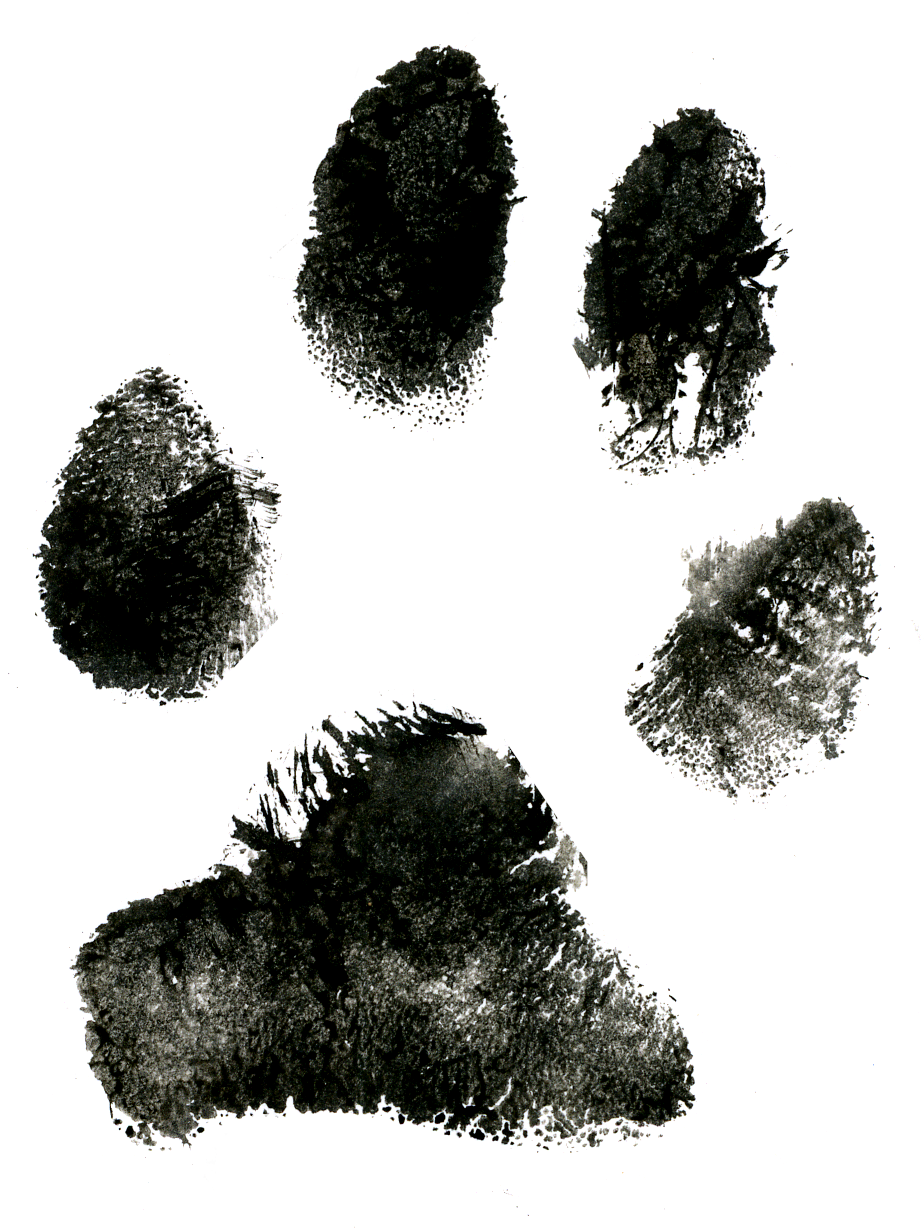
\includegraphics[width=0.5cm]{assets/zpaw.png}
  \end{center}
}

\newcommand\storydiv{
  \begin{center}
    \null
    \vfill
    
\includegraphics[width=1.7cm]{assets/2zpaw.png}
    \vfill
  \end{center}
}

\hyphenation{
\AuthorFirst
\AuthorLast
\Title
\Subtitle
}


\begin{document}
  \nopartblankpage
  \makeatletter
  \renewcommand*{\beforepartskip}{\null\vfill\thispagestyle{empty}}
  \renewcommand*{\afterpartskip}{\par\vskip1cm%
  \@afterindentfalse\@afterheading}
  \makeatother
  \setcounter{part}{0}

  \frontmatter

  \thispagestyle{empty}
  \null
  \vfill
  \begin{flushright}
    \DisplayFont Post-Self
  \end{flushright}
  \vfill
  \cleardoublepage

  \pagestyle{plain}

  \doublespacing

  \begin{flushright}
    \null
    \vfill
    {\Huge\DisplayFont Post-Self}

    \vfill

    {\Large\DisplayFont Madison Scott-Clary}
  \end{flushright}
  \thispagestyle{empty}

  \newpage

  \singlespacing
\thispagestyle{empty}
\begin{center}
    \noindent {\DisplayFont Also by Madison Scott-Clary}
    \TitleFamily

    \vspace{2ex}

    \emph{Arcana — A Tarot Anthology}, ed.

    \vspace{1ex}

    \emph{Rum and Coke — Three Short Stories from a Furry Convention}

    \vspace{1ex}

    \emph{Eigengrau — Poems 2015-2020}

    \vspace{1ex}

    \emph{ally}

    \vspace{2ex}
    
    \textbf{Post-Self}

    I. \emph{Qoheleth}

    II. \emph{Toledot}

    III. \emph{Nevi'im}

    IV. \emph{Mitzvot}

    \vspace{2ex}

    \textbf{Sawtooth}

    \emph{Restless Town}

    \emph{A Wildness of the Heart}

    \vspace{2em}

    Learn more at \emph{makyo.ink/publications}
\end{center}
\vfill
\singlespacing
{\small\parindent0pt\parskip5pt
\noindent Copyright \copyright\ 2020, Madison Scott-Clary. This work is licensed under the Creative Commons Attribution 4.0 International License. To view a copy of this license, visit \mbox{\emph{creativecommons.org/licenses/by/4.0/}} or send a letter to Creative Commons, PO Box 1866, Mountain View, CA

\vspace{1ex}

ISBN: \ISBN

\vspace{1ex}

\textit{Nevi'im}

\vspace{1ex}

Cover \copyright\ Iris Jay, 2022 --- irisjay.net

\vspace{1ex}

%\textit{This digital edition has been posted to Internet Archive and OpenLibrary by the author.}

\Edition\ Edition, \Year. All rights reserved.

\vspace{1ex}

This book uses the fonts Gentium Book Basic, {\DisplayFont Gotu} and {\TitleFont Linux Biolinum O} and was typeset with {\usefont{OT1}{cmr}{m}{n}\XeLaTeX}.

%Printed in the United States of America\\
%\EditionsList
}%\parindent0pt

\clearpage


  \setcounter{tocdepth}{-1}
  \tableofcontents*
  \newpage
  \null
  \cleardoublepage

  \mainmatter

  \pagestyle{ourbook}

  \cleardoublepage
  \markboth{Qoheleth}{}
  \book{Qoheleth}

  \addcontentsline{toc}{part}{Qoheleth}
  \part*{Qoheleth}
  \null
  \thispagestyle{empty}
  \vfill
  \begin{quote}
    \emph{Whatever is has already been, and what will be has been \mbox{before;} and God will call the past to account.}

    --- Ecclesiastes 3:15
  \end{quote}
  \vfill
  
  \hypertarget{true-name-2124}{%
\chapter{True Name—2124}\label{true-name-2124}}

The next meeting spot for the Council of Eight was in a rooftop bar. However, given that that rooftop bar was in the midst of a block of apartment buildings and vertical malls that had built with shared walls, such that there was a cubic half-mile of stair-climbing, elevator rides---down as well as up---and trestles that bridged buildings of lower height than higher ones, it was more adventure getting to the venue than the meeting itself promised.

Still, The Only Time I Know My True Name Is When I Dream climbed.

The apartment buildings ranged from serviceable to gutted, and more than one time, she had to step carefully through a path covered in rubble. She could not decipher whether this was due to abandoned renovations, some unknown battle, or the simple degradations of time.

The malls offered different dichotomies. Some of them were sparkling new with speakers that whispered to her in Mandarin and lights that shouted in her face, while others played placid muzak through halls lit only by emergency lights, darkened storefronts yawning onto scuffed and over-waxed parquet floors.

She wondered who it was that had owned this sim, what collective it was that had decided to mash all the best and worst multiple clashing centuries worth of Kowloon Walled City and the North American Central Corridor.

And then, the rooftop bar. Despite no vehicle entrance to the complex, this was situated on the top level of what appeared to be a car park straight out of a mid-western American airport, complete with one or two of those vehicles that seemed perpetually parked, ones that had lingered for months or years, accruing a parking debt of thousands, tens of thousands of dollars.

The bar itself was a pop-up affair, with walls and ceiling of corrugated plastic held together with rivets and tape, a bar-top that was a few two-by-eights set across a trestle, fronted with further corrugated plastic to keep the patrons from kicking fridges or sinks out of alignment.

The drinks: early 2100s hipster bullshit, all intensely sweet or riddled with smoke-scented fizzy water or long strips of seaweed or clams within the ice cubes, steadily making the drink more and more savory over time.

True Name found it all confusing and jarring.

She liked it immediately.

Debarre was already at one of the tables---similarly cobbled together---sipping something that seemed to be all foam. He waved to her as she entered, and she waved back, heading to the bar to pick up one of those seaweed concoctions before joining him.

``That looks fucking gross, Sasha.''

She laughed and shrugged. ``I am True Name, but yes, it really does. If we are going to meet in a place that gives me a headache to walk through, it is probably best that I get something with\ldots protein? Is that how this works?''

``Uh, sorry. Yeah. True Name.'' The weasel splayed his ears and averted his eyes. ``Can we talk about that sometime?''

``Yes, but probably as Michelle, if that is okay.''

``Why?''

``She is\ldots closer to it than I am.''

Debarre gripped his glass more tightly and twisted sideways to swing his leg over the bench and straddle it. ``Yeah, I don't get it. Before everyone else gets here, can you at least give me a sentence or two?''

``When she forked, when I\ldots became me, she decided not to fork that part of her that suffers if that is the right word.'' True Name frowned. ``Already we are drifting further apart. The species remains, the appearance and the speech patterns remain, the \emph{mind} remains, but not that part of her that is so split. I am me, I am templated off of Sasha, because being both Michelle and Sasha at the same time was no longer tolerable.''

He shrugged, still staring down into his drink. ``I can't speak to that, I guess. But why Aw--''

True Name slammed her glass down on the table a bit harder than intended, some of the drink spilling over her hand. ``Do not say that fucking name.''

The weasel jumped at the sudden intensity, and when he recovered, he finally met her gaze. His expression softened from fear and anger to a tired bleakness. That moment drew out for a long few seconds of quiet and seething sadness. He reached for a napkin from the dispenser at the end of the table and handed it to her. ``Here.''

She hesitated, mastered a surge of unnamed emotion, and accepted the napkin to wipe the sticky drink from her paw and then, on realizing that she was crying, the tears from her face. ``Sorry, I am just\ldots{}''

``We'll talk.'' He reached over and gave her dry paw a squeeze in his own. ``Michelle and I will. There's something I'm missing here is all, and I want to figure out why more than what.''

True Name hid her muzzle in her drink and pretended to take a sip until she was sure she wouldn't slur her words when she spoke. ``Thank you. She is open to messages still, I will let you two work it out. For now, I need to focus on the meeting. Jonas and Zeke are here.''

Looking over his shoulder, Debarre nodded and turned to sit on the bench to face her again, leaving room for the other two. Jonas settled next to True Name so that they could give their speech together when the time came, and Zeke, that shifting bundle of rags and grime slid onto the bench beside Debarre.

``Good afternoon,'' the almost-face within the bundle rasped.

Jonas grinned. ``It's morning, isn't it?''

A pseudopod that may have been a hand waved the comment away. ``Time has lost all meaning. I seem to have forgotten how to sleep, these days.''

``You need a vacation like Michelle.''

There was a low rattle from the rags, and True Name imagined that must be Zeke's laughter. ``Don't tempt me. I don't have the funds to fork, so you'd be down to seven.''

``Why \emph{did} you make it so expensive?'' Jonas elbowed True Name in the side.

She held up her paws defensively and laughed. ``I did not. The price is tied to system capacity.''

``The laws of physics were a mistake and reputation is a lie.''

``It is the best limiting factor that we have that is not a complete fabrication, at the moment.''

``I rather miss coins.''

``My dad used to collect coins, you know.''

And so on, until the table was full and the cone of silence fell.

``Sasha? Uh\ldots True Name. Jonas?'' one of the well-dressed triad asked.

``Right,'' Jonas said, setting his drink down. ``The bill. Things are progressing slowly, as they always do, but it sounds like they might start picking up steam shortly. Our main contact on the DDR side, one Yared Zerezghi based out of the Northeast African Coalition, says that some of the governments are starting to take interest in the bill, which could work to our advantage. Having it just be a direct vote would mean that we would have far, far more representatives to convince, since that'd mean essentially everyone on the DDR. The more governments in play, the more the role of the DDR shrinks.''

``How does that even begin to help? Aren't they super stodgy?'' Debarre asked.

``They can be,'' Jonas hedged. ``But if we can form contacts with each of them, we can argue our case directly. Yared might be the one to give us a good in for the NEAC, and I still have some Western Fed contacts.''

``Anyone for the S-R Bloc or anywhere in SEAPAC? Middle east? India?''

The trio of suits raised their hands. ``S-R Bloc. We don't know any of the oligarchs directly, but we had some big money interests of our own.''

``Israel,'' Zeke said, then laughed at the awkward silence that followed. The trio frowned. ``Sorry, nothing to be done there.''

``And SEAPAC?''

user11824 shrugged. ``I was a nobody, but I was a Maori nobody.''

``You had enough to upload. That has to count for something, doesn't it?''

He shrugged again.

``We will take all the help we can get,'' True Name said. ``Even from nobodies.''

``Alright, I'll poke mom.''

Zeke nodded to True Name. ``What's your take on the situation?''

She stirred her drink to buy herself some time to think. ``I think it is leaning our way. One of the big arguments remains speciation, but Yared's turning that into a pro-rights argument instead of a neutral- or anti-rights one. His voice is getting louder, too. It sounds like he is getting a lot more upvotes on his posts than before.''

``That's good.''

True Name nodded. ``I think so. He is not the biggest voice on the issue yet, but it sounds like he is probably in the top three.''

``You said he's NEAC, right?''

``Yeah, Addis Ababa,'' Jonas said. ``Not exactly the seat of power, but I guess not everything has to be Cairo. Sounds like we have a good mix, at least. No one from South America?''

Everyone shook their heads.

``I suppose that's alright. They're a big enough voice in Western Fed, but they're still in the shadow government side of things. They don't even have the shadow minister of System affairs.''

``Who does?''

``Lithuania.''

One of the suits laughed, and Debarre looked blank.

``Politics,'' Jonas said, grinning lopsidedly.

``If you say so.''

After a moment's silence, Zeke rasped, ``So what are our next steps?''

``Let's all talk to our respective interests---Zeke too---and we'll meet again soon. True Name and I will keep working with Yared and guide as best we can from our side. Speaking of, though, any thoughts on the speciation topic?''

Six sets of eyes flitted between Debarre and True Name, between weasel and skunk, then the whole council laughed.

``I don't give a shit,'' user11824 said. ``But if your Yared guy can twist that argument against the opposition, then that's just one more tool, isn't it?''

``We aren't seeing that,'' the man in the suit spoke up. ``Two thirds of our power structure still think child restrictions are a good enough idea that those laws have bled into Russia. I'm pretty sure they see speciation as a positive. What better way to help in population control?''

One of his companions shrugged, ``I wouldn't be surprised if they started putting limitations on uploading by gender, but that is a separate topic.''

``Zeke?''

The pile of rags shifted in a shrug.

``Debarre? True Name? Anything you can leverage?''

The weasel laughed. ``I mean, if you want to point to us as an example to push that along, and Yared's tack seems to be working, go for it.''

``Alright. It's something you can suggest to your respective interests if you think it'll help. We'll reevaluate next meeting. Anything else on the agenda?''

Everyone shook their heads, then lifted their glasses to a toast. The cone of silence dropped.

``Well, then, you are all free to stick around or go if you want,'' True Name said. ``I am going to stay and get well and truly plastered.''

  \hypertarget{codrin-bux103lan-2346}{%
\chapter{Codrin Bălan — 2346}\label{codrin-bux103lan-2346}}

It took both both eir partners to talk Codrin down from eir desire to simply get right to work.

\emph{``My dear, if, as he said, Tycho was going to take a nap, perhaps you ought to do the same.''}

``I know,'' ey replied, shoulders sagging. ``It's hard to get out of that mindset of having to just work.''

``I know it's enjoyable,'' the fox's partner said. ``But seriously, Codrin, even if you're not going to take a nap, take a thermos out onto the prairie and walk for a bit. Tycho is going to need quite a bit of help, given what you told us of him--''

\emph{``And if True Name is already involved.''}

``That too, yeah. So it's probably best to go into the whole thing prepared for jittery astronomers and\ldots well, whatever True Name is, these days.''

Codrin nodded. ``That makes sense, at least. Do we even have a thermos?''

``Probably. I'll go digging. Might as well make a fresh pot, while I'm up.''

\emph{``You, my love, are a true delight,''} Dear said, tail flitting this way and that.

They grinned, walked off to the kitchen, and started clattering around in cupboards for a coffee therm.

``Dear, have you talked to True Name recently?'' Codrin asked after a polite pause.

It shook its head. \emph{``Not in terms of a conversation, at least. I have received a few messages from her in the intervening years, several of which were sent to several Odists as a group.''}

``She does that? What are they? Orders or something?''

It shook its head, ears flapping slightly at the movement. \emph{``No.~Or, well, not exactly. They are simply updates, or replies to other, ongoing conversations. Many of us still communicate with each other on a somewhat regular basis, and I have been looped into several of those conversations over the years.''}

``Wait,''not exactly``?''

\emph{``You have met her. She does not need to order, oftentimes. She simply suggests.''}

Ey frowned. ``I sometimes worry that we've been attributing almost magical manipulative abilities to her, honestly.''

Dear shrugged. \emph{``Perhaps, but she also has had more than two hundred years of study under her belt to find all of the best ways to interact with people. May Then My Name was something of a let-down for her, I think, even from the very beginning, so she had to learn to take on that mantle herself.''}

``Especially over the last few years, you mean? With Ioan?''

\emph{``Perhaps, though I think that might be ancillary to the fact that our dear May is not on the LVs at all.''}

Ey blinked, laughed. ``Okay, well, fair. I'd almost forgot.''

The fox gave em a strange look. \emph{``You forgot that May Then My Name was not here?''}

Their partner showed up, a cup of coffee in one hand and a (far too large) thermos in the other. ``Are you forgetting things again, Codrin?''

``No, no,'' ey said, accepting the thermos with a frown. ``Or, well, kind of. I didn't forget that May Then My Name wasn't here, just the ramifications of that, that True Name might not have her as a tool.''

\emph{``That is more understandable, yes,''} the fox said. \emph{``Perhaps the True Name here on Castor has diverged from that on the L5 System in that respect, perhaps not. I suspect that both are disappointed, in their own ways.''}

Codrin fiddled with the thermos, ensuring that the lid was a mug when removed — two nested ones, actually — then nodded, standing. ``I don't know how many dimensions she's thinking on, but I also wouldn't be surprised if she had a cost-benefit analysis on losing her to Ioan.''

\emph{``I would not be surprised, no, which would mean that she has planned around that eventuality. I am sure that May Then My Name is keeping an eye on that. Do not let us keep you, though, my dear. Go for your walk. Think about something else. Enjoy the cold, build a cairn around your worries, and then return safe.''}

Ey smiled, leaned down to kiss the fox between the ears, then eir other partner on the cheek. ``I didn't know that was possible, but I'll try. Back in a bit.''

Ey made it two cairns out before caving to the desire to simply get started, and stepped over to Tycho's field. There was a ping of amusement from Dear, to which ey replied with a guilty apology and an acknowledgement that ey'd return soon, all while waiting for eir eyes to adjust to the sudden darkness.

The next sensorium message was a gentle ping to Tycho — nothing so loaded with anxiety as the one ey'd received this morning, just an acknowledgement, a view of the stars.

A voice came from somewhere behind em. ``Codrin?''

Ey whirled around to see a dim cone of red light shining on the ground, illuminating feet in a pair of well-worn boots. ``Tycho? Sorry for intruding like this. I hope I'm not waking you or anything.''

``No, no. Come in. I haven't been able to sleep since True Name left.''

There was a small click and then a ray of further red light spread out from a doorway, showing a small hut nestled within the trees. Ey let emself be guided into the door, finding a sparsely decorated room — a desk, a bed, and a massive cork board nailed to the wall, covered in at least three overlapping layers of notes.

``Thanks for having me,'' ey said, sitting on the offered chair while Tycho claimed the edge of the bed. Once the door was shut, a switch shifted the red light to a normal, warm desk lamp. ``I should've mentioned that I'd be coming over, first.''

He waved away the apology. ``I knew you'd be here, though I didn't know when.''

Codrin paused in the middle of unscrewing the lid to the thermos. ``You knew?''

``True Name said you would.''

Ey frowned, finishing opening the thermos and offering Tycho one of the two mugs of coffee. ``What did she say about me?''

``She didn't talk with you?''

Ey shook eir head. ``Did she say she would?''

Tycho sipped at the coffee, winced, and set the mug aside to cool. ``No, she just talked as though she had, or at least that she knew you'd be working with me.''

``Of course she did,'' ey murmured. ``She knows me too well.''

The astronomer ground the heels of his palms against his eyes. ``I feel like she knew me too well, too. We had what felt like a wonderful conversation where she offered me a job, asked me to fork to send an instance with her to keep working with her, but then quoted some bit of poetry at me and I couldn't tell if it was a death threat or a warning or whatever. I'm still trying to recover from that.''

``I'm guessing you said yes to both the job offer and the fork?''

He nodded. ``It all just sounded so normal. There didn't seem like anything else to do.''

``Can you tell me more about both?''

``Well, she said that she a good deal about the communications and that she'd like me to come help her with the mechanics of that. She'd help me out with resources and I'd teach her about Artemis as I learned it.''

``Artemis? Is that what they're calling the remote\ldots ship? Vehicle?''

He nodded. ``Vehicle, I think. She said they're calling it Artemis, that I should tag my fork \#Artemis, and that those on the ship were either Artemisians or Sea People, which I didn't get.''

Codrin leaned back in the seat, thinking. ``Sea People might be a reference to something from the Mythology, or it could be a reference to a theory about a marauding group of seafarers during the Bronze Age collapse. There was a bunch of talk about how this group had sacked much of the ancient near east and northern Africa, leading to the prolongation of the collapse.''

Tycho's eyes grew wide. ``Do you think that's what she's getting at with the reference? That these are going to be some marauders coming to mess with the LV?''

Ey shrugged. ``Who knows. Probably both, honestly. Maybe there's even some reference that we're missing. She's True Name, there really is no way of telling.''

Nodding, Tycho scooted back on the bed until his back was to the wall, then brought his knees up to his chest. He looked small to Codrin, somehow diminished after the events of the last\ldots goodness, had it only been a day? Diminished, yes, and younger, though he'd always looked as though he was not yet out of his forties in his well-groomed salt-and-pepper hair and well-kept beard.

They sat in silence for a while. Codrin could not guess what the astronomer was thinking about, though ey could see his eyes occasionally darting this way and that, as though connecting one idea to another in the air as well as in his head.

On eir part, ey began structuring the project. There would have to be the journalistic aspect of it, much closer to that of the Qoheleth project than the History, but if the conservative Odists were also involved, there'd likely also be far more observing than researching.

``Tycho,'' ey said, startling him out of a reverie. ``Do you know what an amanuensis is?''

``Like a recorder? Someone who takes notes?''

``Well, in part, but also someone who thinks about what they're writing,'' ey said, tapping at eir temple. ``They aren't a scribe or a court recorder, but someone there to witness and digest a conversation.''

``Like a clerk?'' He grinned. ``We used to have one of those for our club, who would take minutes of the meetings and such.''

Ey nodded. ``Certainly closer to that than a recorder, yeah. I bring this up because that will be my job in all of this, but I think it'll also be yours. Things like the History are all well and good, and I loved putting the work into it, but I also really enjoy doing this. I may wish that the things I get caught up in weren't always so dramatic, but I'll take what I can get.''

``What do you mean, it'll be my job too?'' he asked.

``Just that you will also be witnessing and thinking about this project, and then coming up with ideas related to it to be compiled into a coherent understanding. That's why we'll be working together, I think. I'm trained to do this work in particular, but I'll need your help in making sense of it. I'll experience it with you as much as I'm allowed, but you'll have to ensure that I actually understand what's going on.''

Tycho laughed. ``Well, I'll do my best, but it's not like I have much experience working with Artemisians, either. I'll help with the technical aspects as best I can, though.''

``Excellent,'' Codrin said. ``Thank you for that. I'll be managing most of that, so you won't have to worry too much about the minutiae, but I figured it'd give you a better idea of what to expect when we work together.''

He nodded.

``On that note, lets come up with a basic idea of our next steps. We mostly talked about immediate next steps, but it might be a good idea to start thinking on a larger timescale.''

``I guess. I'm assuming it'll be pretty loose, given that we can't guess the particulars?'' He waited for Codrin to nod, then continued. ``Then I guess we have a few weeks before they reach their closest approach as long as we both stay on our own heading.''

``Does that mean a few weeks before they upload?''

He shrugged. ``Not necessarily. They can upload whenever they want, so long as our Ansible is on and the DMZ is ready. I don't think it's on, yet, though.''

``Alright. Have we received any further communications from them? Their message said that they had a similar mechanism in place. Is that something we'll be able to use? Or even want to use?''

``No further communications that I know of,'' he said. ``But True Name said that all communications will be gated through her, and I don't know if that means that I'll be getting them or just Tycho\#Artemis. Hopefully both, if you and I are to be working on this as well.''

Codrin frowned. ``Well, okay.''

``As for us using their mechanism, I guess it depends on if it's something we can reconfigure our Ansible to use, or if we will need to construct something new. If we'll need to construct something new, then we might not be able to do so in time. Our manufactories are meant for repairs rather than construction. Theoretically they could be used for such, but I don't know how long that'd take without someone phys-side to help.''

``And would we want to?''

``That feels like a question for True Name, not me,'' he said after a long pause.

Ey finished eir coffee and replaced the cup on the cap of the thermos. ``One of us will have to work up the courage to ask her, sometime. But for now, is it something you would want to do?''

``What? Upload to Artemis?'' He looked startled by the question.

``Yes. If it's possible, I mean. I figure it could just be an instance rather than completely investing, though I'd also be curious to hear your opinions on that.''

Tycho tilted his head back until it hit the wall of the hut, staring up toward the ceiling. He sat like that for a good five minutes, during which Codrin remained silent, before leaning forward to grab his cup of coffee now that it had cooled down. ``Yes. I don't know that I'd invest completely, but yes, I think I would. Would you?''

Ey smiled, though ey felt just how tired ey was as ey did so. ``Perhaps. I have attachments here, though. So the Codrin who uploaded — if ey remains a Codrin — would be severed completely from those ey loves. As romantic as the idea of sailing away on some alien spacecraft might be, it'd be painful to leave, even knowing that a Codrin remained.''

``And if your partners uploaded with you?''

The thought caught em up short, and several trains of thought crunched to a halt within em. ``If they\ldots{}'' Ey laughed, shaking eir head. ``You know, I hadn't considered that, yet. I wonder why? But yes, if they chose to do so, then yes, I'll go with them.''

The conversation wound on from there, picking apart a few possible next steps that lay ahead of them, but throughout it all, at least one thread of eir mind was dedicated to picking at that question.

Why had ey not considered whether or not Dear and its partner would want to upload? It wasn't as though ey didn't attribute the agency to do so to them, ey knew just how independent and intelligent they were on their own. Nor was it that ey hadn't made any guesses as to whether or not they would — ey suspected that Dear would jump at the opportunity.

The root of the issue lay within emself, ey knew. Why was ey not able to make that decision without them doing so first? Was ey really such a follower? Or, to put it in a way that was more kind to emself, was ey really so stuck living five minutes behind them that ey couldn't imagine making the decision in the face of the possibility of simply reacting to it? Would ey be able to say yes or no to that question if they asked?

Would ey be able to argue one way or the other, to convince them to come with em or not?

  \hypertarget{true-name-2124}{%
\chapter{True Name—2124}\label{true-name-2124}}

The next meeting spot for the Council of Eight was in a rooftop bar. However, given that that rooftop bar was in the midst of a block of apartment buildings and vertical malls that had built with shared walls, such that there was a cubic half-mile of stair-climbing, elevator rides---down as well as up---and trestles that bridged buildings of lower height than higher ones, it was more adventure getting to the venue than the meeting itself promised.

Still, The Only Time I Know My True Name Is When I Dream climbed.

The apartment buildings ranged from serviceable to gutted, and more than one time, she had to step carefully through a path covered in rubble. She could not decipher whether this was due to abandoned renovations, some unknown battle, or the simple degradations of time.

The malls offered different dichotomies. Some of them were sparkling new with speakers that whispered to her in Mandarin and lights that shouted in her face, while others played placid muzak through halls lit only by emergency lights, darkened storefronts yawning onto scuffed and over-waxed parquet floors.

She wondered who it was that had owned this sim, what collective it was that had decided to mash all the best and worst multiple clashing centuries worth of Kowloon Walled City and the North American Central Corridor.

And then, the rooftop bar. Despite no vehicle entrance to the complex, this was situated on the top level of what appeared to be a car park straight out of a mid-western American airport, complete with one or two of those vehicles that seemed perpetually parked, ones that had lingered for months or years, accruing a parking debt of thousands, tens of thousands of dollars.

The bar itself was a pop-up affair, with walls and ceiling of corrugated plastic held together with rivets and tape, a bar-top that was a few two-by-eights set across a trestle, fronted with further corrugated plastic to keep the patrons from kicking fridges or sinks out of alignment.

The drinks: early 2100s hipster bullshit, all intensely sweet or riddled with smoke-scented fizzy water or long strips of seaweed or clams within the ice cubes, steadily making the drink more and more savory over time.

True Name found it all confusing and jarring.

She liked it immediately.

Debarre was already at one of the tables---similarly cobbled together---sipping something that seemed to be all foam. He waved to her as she entered, and she waved back, heading to the bar to pick up one of those seaweed concoctions before joining him.

``That looks fucking gross, Sasha.''

She laughed and shrugged. ``I am True Name, but yes, it really does. If we are going to meet in a place that gives me a headache to walk through, it is probably best that I get something with\ldots protein? Is that how this works?''

``Uh, sorry. Yeah. True Name.'' The weasel splayed his ears and averted his eyes. ``Can we talk about that sometime?''

``Yes, but probably as Michelle, if that is okay.''

``Why?''

``She is\ldots closer to it than I am.''

Debarre gripped his glass more tightly and twisted sideways to swing his leg over the bench and straddle it. ``Yeah, I don't get it. Before everyone else gets here, can you at least give me a sentence or two?''

``When she forked, when I\ldots became me, she decided not to fork that part of her that suffers if that is the right word.'' True Name frowned. ``Already we are drifting further apart. The species remains, the appearance and the speech patterns remain, the \emph{mind} remains, but not that part of her that is so split. I am me, I am templated off of Sasha, because being both Michelle and Sasha at the same time was no longer tolerable.''

He shrugged, still staring down into his drink. ``I can't speak to that, I guess. But why Aw--''

True Name slammed her glass down on the table a bit harder than intended, some of the drink spilling over her hand. ``Do not say that fucking name.''

The weasel jumped at the sudden intensity, and when he recovered, he finally met her gaze. His expression softened from fear and anger to a tired bleakness. That moment drew out for a long few seconds of quiet and seething sadness. He reached for a napkin from the dispenser at the end of the table and handed it to her. ``Here.''

She hesitated, mastered a surge of unnamed emotion, and accepted the napkin to wipe the sticky drink from her paw and then, on realizing that she was crying, the tears from her face. ``Sorry, I am just\ldots{}''

``We'll talk.'' He reached over and gave her dry paw a squeeze in his own. ``Michelle and I will. There's something I'm missing here is all, and I want to figure out why more than what.''

True Name hid her muzzle in her drink and pretended to take a sip until she was sure she wouldn't slur her words when she spoke. ``Thank you. She is open to messages still, I will let you two work it out. For now, I need to focus on the meeting. Jonas and Zeke are here.''

Looking over his shoulder, Debarre nodded and turned to sit on the bench to face her again, leaving room for the other two. Jonas settled next to True Name so that they could give their speech together when the time came, and Zeke, that shifting bundle of rags and grime slid onto the bench beside Debarre.

``Good afternoon,'' the almost-face within the bundle rasped.

Jonas grinned. ``It's morning, isn't it?''

A pseudopod that may have been a hand waved the comment away. ``Time has lost all meaning. I seem to have forgotten how to sleep, these days.''

``You need a vacation like Michelle.''

There was a low rattle from the rags, and True Name imagined that must be Zeke's laughter. ``Don't tempt me. I don't have the funds to fork, so you'd be down to seven.''

``Why \emph{did} you make it so expensive?'' Jonas elbowed True Name in the side.

She held up her paws defensively and laughed. ``I did not. The price is tied to system capacity.''

``The laws of physics were a mistake and reputation is a lie.''

``It is the best limiting factor that we have that is not a complete fabrication, at the moment.''

``I rather miss coins.''

``My dad used to collect coins, you know.''

And so on, until the table was full and the cone of silence fell.

``Sasha? Uh\ldots True Name. Jonas?'' one of the well-dressed triad asked.

``Right,'' Jonas said, setting his drink down. ``The bill. Things are progressing slowly, as they always do, but it sounds like they might start picking up steam shortly. Our main contact on the DDR side, one Yared Zerezghi based out of the Northeast African Coalition, says that some of the governments are starting to take interest in the bill, which could work to our advantage. Having it just be a direct vote would mean that we would have far, far more representatives to convince, since that'd mean essentially everyone on the DDR. The more governments in play, the more the role of the DDR shrinks.''

``How does that even begin to help? Aren't they super stodgy?'' Debarre asked.

``They can be,'' Jonas hedged. ``But if we can form contacts with each of them, we can argue our case directly. Yared might be the one to give us a good in for the NEAC, and I still have some Western Fed contacts.''

``Anyone for the S-R Bloc or anywhere in SEAPAC? Middle east? India?''

The trio of suits raised their hands. ``S-R Bloc. We don't know any of the oligarchs directly, but we had some big money interests of our own.''

``Israel,'' Zeke said, then laughed at the awkward silence that followed. The trio frowned. ``Sorry, nothing to be done there.''

``And SEAPAC?''

user11824 shrugged. ``I was a nobody, but I was a Maori nobody.''

``You had enough to upload. That has to count for something, doesn't it?''

He shrugged again.

``We will take all the help we can get,'' True Name said. ``Even from nobodies.''

``Alright, I'll poke mom.''

Zeke nodded to True Name. ``What's your take on the situation?''

She stirred her drink to buy herself some time to think. ``I think it is leaning our way. One of the big arguments remains speciation, but Yared's turning that into a pro-rights argument instead of a neutral- or anti-rights one. His voice is getting louder, too. It sounds like he is getting a lot more upvotes on his posts than before.''

``That's good.''

True Name nodded. ``I think so. He is not the biggest voice on the issue yet, but it sounds like he is probably in the top three.''

``You said he's NEAC, right?''

``Yeah, Addis Ababa,'' Jonas said. ``Not exactly the seat of power, but I guess not everything has to be Cairo. Sounds like we have a good mix, at least. No one from South America?''

Everyone shook their heads.

``I suppose that's alright. They're a big enough voice in Western Fed, but they're still in the shadow government side of things. They don't even have the shadow minister of System affairs.''

``Who does?''

``Lithuania.''

One of the suits laughed, and Debarre looked blank.

``Politics,'' Jonas said, grinning lopsidedly.

``If you say so.''

After a moment's silence, Zeke rasped, ``So what are our next steps?''

``Let's all talk to our respective interests---Zeke too---and we'll meet again soon. True Name and I will keep working with Yared and guide as best we can from our side. Speaking of, though, any thoughts on the speciation topic?''

Six sets of eyes flitted between Debarre and True Name, between weasel and skunk, then the whole council laughed.

``I don't give a shit,'' user11824 said. ``But if your Yared guy can twist that argument against the opposition, then that's just one more tool, isn't it?''

``We aren't seeing that,'' the man in the suit spoke up. ``Two thirds of our power structure still think child restrictions are a good enough idea that those laws have bled into Russia. I'm pretty sure they see speciation as a positive. What better way to help in population control?''

One of his companions shrugged, ``I wouldn't be surprised if they started putting limitations on uploading by gender, but that is a separate topic.''

``Zeke?''

The pile of rags shifted in a shrug.

``Debarre? True Name? Anything you can leverage?''

The weasel laughed. ``I mean, if you want to point to us as an example to push that along, and Yared's tack seems to be working, go for it.''

``Alright. It's something you can suggest to your respective interests if you think it'll help. We'll reevaluate next meeting. Anything else on the agenda?''

Everyone shook their heads, then lifted their glasses to a toast. The cone of silence dropped.

``Well, then, you are all free to stick around or go if you want,'' True Name said. ``I am going to stay and get well and truly plastered.''

  \hypertarget{ioan-bux103lan-2346}{%
\chapter{Ioan Bălan — 2346}}
\markboth{Ioan Bălan — 2346}{}

\begin{center}
\emph{Convergence T-Plus 28 days, 13 hours, 35 minutes}\\
\emph{(Castor--Lagrange transmission delay: 30 days, 14 hours, 36 minutes)}
\end{center}

\noindent Ioan knew what was coming, so ey was able to brace emself well enough when May came barrelling out of the default entry point on the dandelion-ridden field that ey was not totally bowled over, managing at least a somewhat graceful descent to the ground. The skunk had already looped her arms around eir middle and tucked her head up under eir chin before ey was even able to sit up straight enough to get eir arms around her.

``You nut.'' Ey laughed, reaching up to tug at one of her ears affectionately. ``Good to see you, too.''

``Ioan, I am in no way sorry for knocking you over,'' she said, voice muffled, her grip around eir middle tightening. ``Though I am dreadfully sorry that this happened again. I missed you.''

Giving up on the prospect of sitting up straight, ey leaned back onto one hand, propping emself up. ``No need to apologize, May. I'm just happy to see you again.''

The skunk leaned away from em enough to dot her nose against eirs. Her eyes were quite red and ey could see tear-tracks in the fur of her cheeks. She looked a mess. ``Do not take my apology away from me. I have been saving that one up.''

``Alright, alright,'' ey said, pressing eir nose a little more firmly to hers for a moment before leaning back again. ``Apology accepted. Are you feeling better?''

She sat upright rather than leaning against eir front and nodded. ``Yes. I was able to get a lot out that I think has been pent up for a while. Thank you for giving me the space. I promise I did not fuck with your pen collection.''

``Good. I had it all perfectly organized.'' Ey plucked a dandelion from the field and tucked it behind her ear. ``Now, do you want to talk about it? Or should we do that later? That was longer than the last few times.''

``Later, please. I want to say hi to Douglas and wash my face and just be normal for a bit.''

Douglas Hadje met them on the stoop of his house and, as had become their ritual over the years, hugged the skunk, lifted, and twirled her around. Her bushy tail streamed along behind her.

``Hey May,'' he said, setting her back down again and kissing her cheek. ``Glad you made it through.''

``Of course I made it through. You still have at least seventy nine years of me haunting you before I can do something else.'' She grinned. ``And even then, the contract is renewable.''

``Ornery as ever.'' He laughed. ``Well, want to come in?''

``For a bit, and then I want to come back out here and lay in the grass and bake in the sun.''

After May had cleaned up and Ioan had helped Douglas prepare coffee and some sandwiches, they sat around the table to catch up.

``So, what news of the aliens?'' Douglas asked.

The skunk squinted at him. ``Has Ioan not been keeping you up?''

``A little. Ey said ey wanted to wait until you got here, though.''

``Whatever.'' She rolled her eyes. ``Well, out with it, then.''

``I've gotten several messages from Codrin over the last few days. Ey said they would be heading out to start the talks in, uh\ldots five days.''

``So they have been into them for a while, now.'' She looked thoughtfully up to the ceiling. ``A few weeks, perhaps?''

``Or maybe they're already over,'' Douglas said.

``A gloomy thought. I would like to hope that they are going quite well. Codrin is there being a Bălan, Tycho is there being a nerd, this Sarah Genet is there being a whatever a Sarah Genet is like, Why Ask Questions is there being a shithead.'' She wrinkled her nose. ``And True Name is doing her best to control the whole thing.''

Ioan was pleased to see the mildness of the skunk's expression. It really did seem like many of those overwhelming emotions had burned themselves out over the last few days.

``It's weird,'' Douglas said. ``Every now and then, I'll hear about something from one of the LVs that's anchored to a certain time and I'll remember, `Oh shit, yeah, they're billions of kilometers away by now', and then I have to spend some time trying to conceptualize that distance.''

Ioan nodded. ``The transmission delay throws a wrench in things, doesn't it? I was just thinking about that on Secession day. We were celebrating and it sounds like they were, too, but we didn't learn about their party until a week later.''

``The thing that always catches me off guard is that our days do not seem to line up any longer,'' May said around a bite of sandwich. ``I mean, they do, but when the delay is off by half a day, we start getting messages at shit o'clock in the morning. It is a strange feeling.''

``Exactly.''

``I hope they're still in the talks, too. Codrin sounded hopeful, at least. The messages that they'd been getting from the Artemisians were interesting, especially the language snippets. I'm guessing the powers that be made em promise not to send the full message text yet, but what they have learned is fascinating. Four races on one ship must be a hell of an experience. The DMZ sim sounds pleasant, though, and all of the work they've done to prepare is really kind of impressive.'' Ey sipped eir coffee to buy a moment's time to think before saying, ``There was a bunch of stuff in there for you, too, May. We can go over that later, though.''

The skunk frowned, finished the last of her sandwich, and then settled back in the chair with her coffee. ``You cannot leave me hanging, my dear. May I at least have a preview?''

``Well, Codrin's worried about you. As is Dear.''

``The memory thing?'' Douglas asked.

Ey nodded.

May averted her gaze, looking out the window to the rolling field beyond. ``I am worried, too. You know that.''

``I know. Reading between the lines, though, I think ey's worried about the whole clade. Ey's worried about you and Dear, and ey's worried about how True Name and Why Ask Questions are going to act through this. Dear reacted poorly to the whole time-modification thing.''

She nodded and sat in silence for a minute before setting her cup down. ``We are not doing as well as many of us would like, no. I have news as well, but I would like to share it outside where I can sit in the sun and feel the grass. Is that okay?''

Ioan and Douglas collected plates and coffee cups, then the three of them trooped out into the field while May spoke.

``We have lost May One Day Death Itself Not Die and I Do Not Know, I Do Not Know. Death Itself stopped talking, and then she stopped moving. In Dreams visited for a while there, and a few days ago asked me to come visit as well. That is why this spell seemed to last longer than usual. Evening hit, she smiled at us, shrugged, and then quit.''

May's voice was thick as she continued. ``They all lived in the same house, did you know that? All ten of that stanza. Many of them did not even talk with each other, and none of them ever forked. They were always quite unstable. The next morning, I Do Not Know was gone, and Names Of The Dead said that she had quit shortly before sunrise.''

Ioan and Douglas remained quiet as they walked. The skunk didn't seem to be quite done saying the things that she needed to.

She continued after a few minutes of mastering emotions, voice clear once more. ``In Dreams and I talked quite a bit. She said that there have been fewer instances of instability in older clades than expected, given \emph{On the Perils of Memory}. Fewer uploads are susceptible to the long-term effects of unceasing memory than expected, I guess. I was pleased to see that Debarre seems to be doing well.''

``That's heartening,'' Douglas said. ``At least in a way.''

The skunk nodded. ``I am pleased that the System is more stable than feared, but I am unhappy that we seem so strongly affected. In Dreams said that she is going to do some research and see if there are ways that we can at least improve on the way we deal with the effects. I do not know that there is a way to get rid of them entirely, at least not without further individuation, but the least we can do is help keep ourselves sane for longer.''

Ioan took her paw in eir hand and lifted it to kiss the back. ``Please, yeah. If you lose it, I'll be furious.''

She laughed and gave em a pitying look. ``Mx.~Ioan Bălan, you are pretty good at acting furious on stage, but I do not believe for a second that you could actually feel that way. Even Codrin was able to have a normal meeting with True Name after she did as she does with em.''

Ey did not laugh. Neither, ey noted, did Douglas.

``I am sorry,'' she murmured, ears laid flat.

``\,`Furious' is the wrong word, May. I'd lose my damn mind.'' Ey took a shaky breath and rubbed at eir face. ``I can't tell you you're not allowed to or anything, since I know it's not really up to you, but please at least try to stick around.''

``I'm not going to pile on or anything,'' Douglas said. ``But I will say I'd be pretty upset, too, so if there's anything I can do to help, I will.''

May dragged them both to a stop in the field. Her expression started out angry, then screwed up into sadness, and finally settled on tired. ``I love you both and I promise I will do what I can to stay here, stay grounded. I cannot speak for the rest of the clade, and certainly not for Dear to soothe Codrin's fears, but I will do what I can.''

It was not uncommon for these reunions to be tearful, Ioan knew, but it was a different sort of pang that settled in eir chest with the news, and it was a few minutes before ey was able to speak again. ``Sorry, you two.''

The skunk stuck her tongue out at em. ``I will allow you this one apology, but do not make a habit of it. You are allowed to cry at sad shit.''

Ey rolled eir eyes and shoved at her.

``Well, I was promised laying in the grass and baking in the sun,'' Douglas said. ``So come on, we can at least enjoy the rest of the afternoon.''

  \hypertarget{qoheleth-2305}{%
\chapter*{Qoheleth — 2305}\label{qoheleth-2305}}

Transcript of Node: \href{http://35.165.134.227/node/bea0cf302fcd00863f0c67a91b1a75c0e4ba4863}{{[}bea0cf302fcd00863f0c67a91b1a75c0e4ba4863{]}} with descriptive text by \#d5b14aa.

\emph{The footage shows two persons. One of them has to be Dear, Also, The Tree That Was Felled, who is an up-tree branch of the Ode clade, eighth stanza. No one else has ears that big, nobody else can somehow speak in italics. The other took some research, but I am confident that ey is an instance of Ioan Bălan, a historian and writer. Ey is a tracker, but only just, as eir habits tend toward few to no long-running instances. This instance is either \#tracker or one tasked to this project.}

\emph{The two persons are sitting outside of a cafe, from whom I obtained this footage. They are in conversation. Going to sit down and watch this.}

\begin{quote}
\textbf{Dear, Also, The Tree That Was Felled}: Thank you for your letter, Ioan. Lots of really good stuff in there, most of which I had missed simply out of nearsightedness.

\textbf{Ioan Bălan}: You've got me hooked on this project, I have to say. It's fascinating stuff.
\end{quote}

\emph{Dear grins at this.}

\begin{quote}
\textbf{Dear} We — that is, some other Odists down-tree from me — have come up with some further hints about the message.

\textbf{Ioan}: Oh? Anything good?

\textbf{Dear}: I suppose it depends on your definition of good.

\textbf{Ioan}: {[}snark, good natured{]} Oh great. Excited already. {[}more earnest{]} The fascination continues. Well, let's have it.

\textbf{Dear}: So, one of us did an exhaustive search of some records and found an old archive server running somewhere.
\end{quote}

\emph{Oh goodie. Better start gearing up.}

\begin{quote}
\textbf{Ioan}: Wait, start at the top. What were they searching?

\textbf{Dear}: They were searching for the block of encrypted text — not what was in it; they cracked that long ago. They searched for the encrypted text itself, and they came across an archive server.

\textbf{Ioan}: Old node boxes? Wow, even I feel crusty using one of those, and I'm a historian.

\textbf{Dear}: {[}laughter{]} They found the archive server though, and there is a bunch of intriguing stuff on it. New, old, the whole thing. There is stuff from ages ago, shortly after we got here, and stuff from a few hours ago.

\textbf{Ioan}: You're kidding. Newly created stuff?

\textbf{Dear}: I know. It is ridiculous.
\end{quote}

\emph{The fox's ears flop when it gets excited and shakes its head, never noticed that. It is kind of cute.}

\begin{quote}
\textbf{Ioan}: Never met anyone who could actually get one working well enough to add new nodes. So the encrypted text was in a node on the server?

\textbf{Dear}: Yes. It is still there. {[}pause{]} Just sent the URI.

\textbf{Ioan}: I\ldots{}well, I'll have to take it at your word that it's the same as the one you found earlier, I'm not going character by character.
\end{quote}

\emph{Dear seems a little frustrated at this. About Ioan's slowness? I know I would not compare the files. It sounds exasperated.}

\begin{quote}
\textbf{Dear}: Of course, Ioan. I promise it is the same, though. Needless to say, we found a crusty old archive with the block on it, and there are other public nodes on there as well. I am guessing a bunch of private ones, too.

\textbf{Ioan}: Anything good in those?

\textbf{Dear}: Nothing\ldots{}penetrable. It is all fairly opaque. To me, at least.
\end{quote}

\emph{Ioan grins at this.}

\begin{quote}
\textbf{Ioan}: Thus us meeting?

\textbf{Dear}: {[}nodding{]} Yes. The only bit that I have any insight into is the deck listing, which I think might be another bit of old encryption--
\end{quote}

\emph{Ioan groans aloud, at which Dear grins.}

\begin{quote}
\textbf{Dear}: My sentiments exactly. It is another encryption scheme which relies on a deck of cards for a stream of random numbers. I have not dug into it in years because the decryption process is so slow, but there may be a node on that box containing the encrypted text.

\textbf{Ioan}: Want me to have a look, then? The techier stuff is going to go right over my head, you know that.

\textbf{Dear}: It is not all tech, promise. I just want you to give it a read and see what you pick up from it, you know? Put your amanuensis hat on and just spend some time experiencing.

\textbf{Ioan}: You think highly of me. No complaints, of course, but I feel I have to ask, why can't someone from your own clade fill this role?
\end{quote}

\emph{Dear is quiet. Struggling for words? Our Dear? This must have hit it hard.}

\begin{quote}
\textbf{Dear}: We\ldots{}differ. The Odists, I mean.

\textbf{Ioan}: ``Differ''? Within the clade?

\textbf{Dear}: Yes. A hallmark of Dispersionistas is that we treat each of our forks as fully-realized individuals. We may have a shared past, but from the point we fork onward, we grow ever further apart.

\textbf{Ioan}: I assume you mean more than just a matter of increasing conflicts.

\textbf{Dear}: Yes. Although we Odists limit our instances to the one hundred available names, we still consider ourselves Dispersionistas as we never merge back down-tree. But, that aside, we also want someone out-clade for this. \emph{I} want someone out-clade for this.
\end{quote}

\emph{Ioan seems taken aback.}

\begin{quote}
\textbf{Ioan}: Do the other Odists not like that I've been brought on?

\textbf{Dear}: Of the ones who know, most are fine with it.
\end{quote}

\emph{Now frustrated/confused.}

\begin{quote}
\textbf{Ioan}: ``The ones who know''?

\textbf{Dear}: You have, of course, noticed that you have not interacted with any of my cocladists. I have told some about hiring you, but not all.

\textbf{Ioan}: Alright, I suppose. If you're independent, then I guess it makes sense that I be your amanuensis rather than the clade's.

\textbf{Dear}: Yes. Perhaps more evidence that we are split on how to tackle this in the first place. Different camps, different strategies, infighting. Ioan, you have to understand that, when a clade gets old, it starts to get a little batty.
\end{quote}

\emph{Calm down fox, I'm working on it. Not so frantic.}

\begin{quote}
\textbf{Dear}: Some clades try to get around this by keeping a certain core group of instances — talking mostly Dispersionistas, mind — in a setting that keeps them as sane as possible. Something that feels very `normal'. Or maybe some are researching forking from earlier points, from down-tree, rather than from where they are now.
\end{quote}

\emph{It furrows its brow.}

\begin{quote}
\textbf{Dear}: We do not. First of all, we started way too early on for that to be a thing. We trusted that change itself would keep us sane, that as instances diverged, especially with mutation algos in place, they would change enough to keep us from falling apart.

\textbf{Ioan}: And that didn't work?
\end{quote}

\emph{Long pause.}

\begin{quote}
\textbf{Dear}: It kind of worked, I will put it that way. I feel fairly well rounded, as much as that means, and I am sure those across the clade from me do too, but it is complicated. You might not recognize my cocladists as Odists without knowing beforehand. It is like having a very close sib that was raised by a different family in a different sim.

\textbf{Ioan}: More different than you'd expect, then?

\textbf{Dear}: `Expect'\ldots{}fits strangely for this. The problem is that they are still \emph{us}, and we are still them. Clades are families of separate individuals in a lot of ways, but you must realize that, in the end, they are still one individual. We are more different than one individual should be. Does that make sense?
\end{quote}

\emph{It does, Dear. That's why I'm doing this.}

\begin{quote}
\textbf{Ioan}: I guess so. {[}pause{]} So some of your clade would prefer I not be a part of this?

\textbf{Dear}: More than that. They feel that investigating the matter of the Name being written is too risky, too close to investigating the Name itself.

\textbf{Ioan}: I don't know how I would respond to that.

\textbf{Dear}: That is my field, Ioan. Do not worry about it.
\end{quote}

\emph{Ioan holds up eir hands, looks apologetic. The fox has tilted its ears back.}

\begin{quote}
\textbf{Ioan}: Sorry, Dear. I hope I'm not overstepping at all.

\textbf{Dear}: {[}calmer{]} Do not worry about it. It is okay, I promise. It is just that we are really good at arguing, so I have been dealing with that quite a bit the last few days. That is why I hired you; I am relegated to an administration role so I am a bit on edge. Let's get back to the archive server, yes?

\textbf{Ioan}: Sure thing. Where did you say your cocladists had found it?

\textbf{Dear}: Just in a search. I do not quite know the details about how. Assuming just a text search of the perisystem. Not too sure on the terminology; I bought into being an artist pretty hard. All that knowledge is in exos.

\textbf{Ioan}: {[}laughter{]} No worries there, Dear. I'm trying to keep up with you is all. I was just wondering if they found anything else.

\textbf{Dear}: You mean like the other nodes on the server?

\textbf{Ioan}: I'll poke around at those, look for ties and such. I was more wondering if they'd found anything in their search that didn't meet the relevancy threshold for them. Stuff like back-links to the server, or anyone talking about this Qoheleth. Hebel. Whichever.
\end{quote}

\emph{Silly name. Oh well. Dear looks taken aback.}

\begin{quote}
\textbf{Dear}: I had not really thought to ask. I do not suppose they did, though. Do you think it is worth having them search around more? Lowering the, uh, relevancy threshold? {[}laughter{]}

\textbf{Ioan}: Yeah, I think so. Though now that I've got it too, I can do some of that digging myself. I want to see who likes the Tanakh so much as to name themselves that. And why `kemmer'.

\textbf{Dear}: I\ldots{}well, it's complicated and out of scope, but it relating to fluidity of gender is relevant to the clade as a whole. Very big for us, if only at a remove. I have opted out.

\textbf{Ioan}: So I noticed. It makes sense, though.

\textbf{Dear}: I am glad someone is thinking about this stuff. You are sounding more like a--

\textbf{Ioan}: Private investigator?

\textbf{Dear}: {[}laughter{]} I was going to say historian, sounding more like an historian every time we talk. But you never know, maybe you would make a good PI.
\end{quote}

\emph{That was fast! I may have less time than I had thought. Dear's lovely, and it's totally right: on the other side of the clade, there are some who'd not like this kind of digging. Too entrenched. Too Conservative.}

\begin{quote}
\textbf{Ioan}: I can't tell whether or not I should be flattered.

\textbf{Dear}: It is a good thing. Just keep digging, and we will too. I will be about. Got a few more things to wrap up to finish the current gallery exhibition, but after that, I am just going to work on this — with you if you do not mind — and try and figure out what is even happening in the clade. Do keep in touch, yes? Ping me whenever.

\textbf{Ioan}: Will do. {[}pause{]} Wait, you're an instance artist, right?

\textbf{Dear}: Yes. Why do you ask?

\textbf{Ioan}: Why don't you fork to work on both at the same time?
\end{quote}

\emph{Dear shrugs, grins, quits. Very lovely fox. Really quite lovely.}

\emph{No time to dawdle watching Ioan try and figure out up-tree instances, though. Must be getting ready. Quit this instance, flush the server of extraneous crap to guide Ioan a little more effectively — yeesh, how old is some of this stuff? Need to re-encrypt a bunch of it anyway — and maybe get ready for some visitors.}

  \hypertarget{rj-brewster-2112}{%
\chapter*{RJ Brewster — 2112}\label{rj-brewster-2112}}

RJ allowed emself to sleep in until near eleven that morning. Last night of dress rehearsal, might as well be well-rested.

Many other members of the troupe held part time jobs during the day, and ey ran a small consulting business of eir own. The more industries that dove into immersive tech, the more eir expertise was worth. Even so, with all that ey did, ey made enough to not have to worry about holding down more than the one full-time gig.

As it was, on days when ey had nighttime rehearsals, ey felt no compunctions about sleeping in. Nothing to be up for, only the 'net to keep them occupied in the mornings, little enough need to get moving.

It was Priscilla who eventually succeeded in waking em, butting her head against eir cheek and purring obscenely, stomping on em through the blanket with kneading paws. The more insistent the cat became, the less able ey was to ignore her intrusions on eir admittedly banal dreams.

Fine. Trudge out of bed. Refill cat's water and food. Give the requisite morning pets to keep her happy. Scoop the litter box. Make self a pot of tea. Tea to shake the grogginess.

Ey sat at the tiny kitchen table, sipping from eir oversized mug and watching the late morning traffic from their window. Mostly business traffic, with the occasional mother with child in tow. Black cabs. Scooters. Bikes.

By the time ey had finished eir first mug of tea, RJ had woken up enough to start on the prowl. As with the night before, ey made sure that everything was in order before touching eir rig. Ey'd taken care of the cat, but ey still needed to eat, emself. So, remembering eir promise, ey set about making a small pot of rice. Fifteen minutes to cook, plenty enough time to finish another mug of tea.

RJ left most of the rice cooling in the pot and took for emself a small bowl to go with the leftover curry. The process of swiping eir hand over the controls of the stove had reminded em of the deck that Sasha had shared last night. There was no reason to think that some random person in London would have much to offer in the case of another person ey had never met getting lost. No reason not to try, though. Maybe there was something, some small insight that ey had which, when pooled with those of others, might help in some way.

So many maybes. So many mights and perhapses.

Empty bowl in sink. Third and final cup of tea in the thick-walled mug. Good enough. Ey allowed emself to settle before eir rig at last.

As before, ey keyed in the password and rested eir hand onto the cradle for the two-factor. However, instead of delving in as ey had last night, ey unfolded the screen to full height and pulled the keyboard closer, swinging the hand rests to the side and the headrest up and out of the way. No need to go immersive, with work like this. Ey could just as easily work as a fox, of course, but it was so easy to lose track of time in there, and the night's rehearsal mustn't be forgotten.

Besides, eir tea was here.

``Let's see,'' ey murmured, taking a sip of tea before setting the mug down

Ey called up Sasha's deck.

\begin{longtable}[]{@{}c@{}}
\toprule
\endhead
Cicero Lost Nov 2111\tabularnewline
Priv eyes only\tabularnewline
See Debarre for ACLs\tabularnewline
\bottomrule
\end{longtable}

\begin{longtable}[]{@{}c@{}}
\toprule
\endhead
Dr.~Carter Ramirez\tabularnewline
specialist in lost\tabularnewline
so. London\tabularnewline
\bottomrule
\end{longtable}

\begin{longtable}[]{@{}c@{}}
\toprule
\endhead
Mr/Mrs.~Jackson\tabularnewline
parents, can't get much more\tabularnewline
dad in govt, mother stays home\tabularnewline
\bottomrule
\end{longtable}

And on it went for nearly a dozen cards. Each had its own cover embossed with a few lines of type, each containing upwards of a gig of information culled from various sources, doubtless of varied quality.

RJ flipped through each, gleaning what ey could from a quick scan, before collapsing the deck once more and sitting back to think. Nothing in there seemed new. Nothing out of place. Ey had only received the deck last night, and yet nothing felt like it had been revealed, uncovered.

Ey knew of the lost, of course, and the name Ramirez was commonly tied with the hundred or so cases that had cropped up over the years. The family\ldots{}no, nothing to be gained there, at least not that had already been tried by Debarre. And again, there was the problem of being a random nobody in the UK: no one known, no one with power.

None of the rest of the cards carried any real significance to em.

If there was anything RJ was going to add to the conversation, it would be through eir connection to Cicero. Something ey knew, something the two had shared.

A small notification slid down from the top of eir monitor, covering the upper right corner of the screen.

\begin{quote}
\textbf{D — D — R}

Voting begins in \emph{5} minutes on \emph{referrendum 238ac9b8}:

Summary: \emph{Tariffs on importation of goods from the Sino-Russian Bloc\ldots{}}

Cost: 1,000

Comment: 150,000

Bounty: 280,000
\end{quote}

RJ reached to swipe the notification away. Ey had very little stake in the uncomfortable alliance between Western Fed and S-R Bloc. Could care less, honestly, about taxes on things that ey'd never buy. Then something clicked within em, and ey halted eir motion.

\emph{Cicero.}

Ey hastily shuffled back through the \emph{Cicero Lost} deck until coming up with the `recent net activity' card and pulled up the contents. It took a few moments to remember how to sort tabular data — database classes in high school so long ago — but eventually, ey got the table sorted around the activity type. Ey scrolled rapidly through the list until ey got to the list of Direct Democracy Representative entries.

There was the connection. The one thing that RJ and Cicero had was their arguments over politics. Not just politics, but the worthiness of the current political system in all of its facets. Arguments upon arguments upon arguments, fennec fox and tabby cat with their ceaseless bickering in the Crown Pub.

RJ was firmly on the left, but ey felt the representative democracy combined with the DDR was a pretty good system. Not great, sure. It was \emph{fine}. It \emph{worked}. To ask for more from a political system was to invite further troubles like those from the preceding century.

Cicero, however, seemed to waver between socialism and anarchy, depending on factors such as how much he had had to drink and how angry he was at the most recent vote.

\emph{I certainly can't see broad shifts going my way,} he had slurred on more than one occasion. \emph{Least I can vote. Vote on every damn thing that comes my way.}

Ey made sure syncing was turned on across all copies of the deck before snipping those rows out of the activity table into a card of their own:

\begin{longtable}[]{@{}c@{}}
\toprule
\endhead
DDR votes\tabularnewline
todo: process by record\tabularnewline
1 month, 835 votes (!)\tabularnewline
\bottomrule
\end{longtable}

The icon in the upper left of the screen showing the deck twirled gracefully to show the sync.

Cicero had voted precisely how he had talked. On the surface, he was no different than any other far-left socialist on the DDR.

Along with the ability to vote on issues directly came the ability to comment — for a price. DDR votes didn't cost money, but they did cost credit, up to 1,000 per. Credit gained by voting on cheaper issues, for each vote provided a bounty paid upon consideration, beginning with a few freebies in the tutorial.

What Cicero's records showed was that he was wealthy. \emph{Fantastically} wealthy. RJ had a few million DDR credits banked away in case a high value issue that ey felt strongly about cropped so that ey could make a comment. Unlike voting, commenting could cost upwards of five million credits. And one could buy their way to influence by flooding issues with comments.

Cicero's wealth surpassed RJ's at least a hundred times over, if not more. Well into the billions of credits. For someone to be as active in commenting as ey knew the cat to be and still have that much in credits stored up showed a dedication to following politics that was just barely hinted at by those tispy rants. Cicero was well connected, well read, and, most importantly, apparently a key political figure on the DDR comment sections to an extent that none of the Crown regulars had ever expected.

RJ sat back in silence for a few moments before muttering, ``Well, shit. Prisca, you don't suppose\ldots{}''

Rather than finishing the thought out loud, ey dashed off a summary in the notes attached to the card.

\begin{quote}
AwDae here. Looks like there's a lot going on in DDR activity (where'd you get this, Debarre?). Cicero was into a lot, and I'm not trying to go all conspiracy nut on you all, but do you think that maybe he got in too deep or something? Not saying someone tried to do it too him or anything, just that maybe the more one uses the net, the more likely it is to happen to them? I mean seriously, look at all of his votes, and his stash of credits! I'll keep poking at this after rehearsal.
\end{quote}

The tea had gone cold long ago, but ey downed it all the same. Ey'd spent longer than planned plowing through the data the hard way and ey risked being late if ey didn't start hustling.

It was nearing dusk by the time ey left, the suit newly brushed and ironed, the gloves newly washed, the RJ newly shaven.

On the way back to the tube station, ey stopped by a Thai counter and picked up a take-away container of noodles for the night. Ey made it halfway through the container before the rancid belch of station wind suggested ey pack it away before heading down to the platform.

Throughout the ride to Soho, RJ's mind continued prowling through the data in Sasha and Debarre's deck. Ey kept mulling over that surreal number of credits. Just how much social currency was bound up within the reputation market of the DDR credit system?

Cicero had built himself up into a proper political player.

  \hypertarget{archive-hebel-qoheleth-node-7cbc92e691678c4c17a04f5553cd1058ee122956}{%
\section{Archive: {[}Hebel Qoheleth{]} \textbar{} Node: {[}7cbc92e691678c4c17a04f5553cd1058ee122956{]}}\label{archive-hebel-qoheleth-node-7cbc92e691678c4c17a04f5553cd1058ee122956}}

{[}Encrypted{]}

\hypertarget{archive-hebel-qoheleth-node-32c5a64b66d0338be4373d796cf1eae5343f1077}{%
\section{Archive: {[}Hebel Qoheleth{]} \textbar{} Node: {[}32c5a64b66d0338be4373d796cf1eae5343f1077{]}}\label{archive-hebel-qoheleth-node-32c5a64b66d0338be4373d796cf1eae5343f1077}}

\begin{verbatim}
OCYNX GRIMN CYJPE PNNXS SCIQZ
KTWQW FBAVY FBOPA QERLB HWIJW
KPELO UCLAN OKHPM PCPWR NZNZQ
NMTIQ BKNGH UWFMG BPPZS CNRKX
TKEMU AFNOS VQUNW
\end{verbatim}

\hypertarget{archive-hebel-qoheleth-node-36b1d8c1df07ce0f254b2332acd38c59bdf3bb00}{%
\section{Archive: {[}Hebel Qoheleth{]} \textbar{} Node: {[}36b1d8c1df07ce0f254b2332acd38c59bdf3bb00{]}}\label{archive-hebel-qoheleth-node-36b1d8c1df07ce0f254b2332acd38c59bdf3bb00}}

{[}Encrypted{]}

\hypertarget{archive-hebel-qoheleth-node-67e97446cdbe3a4a3cfd5ebd75b1260f-error}{%
\section{Archive: {[}Hebel Qoheleth{]} \textbar{} Node: {[}67e97446cdbe3a4a3cfd5ebd75b1260f{]} Error}\label{archive-hebel-qoheleth-node-67e97446cdbe3a4a3cfd5ebd75b1260f-error}}

The node you have requested, {[}67e97446cdbe3a4a3cfd5ebd75b1260f{]}, does not appear to be an Archive node. You have provided a 32 byte identifier; the Archive system uses 40 byte identifiers.

If you believe you have received this message in error, please contact the Archive owner.

If you believe that you have the correct identifier, you may have attempted to access it on the wrong system. Please check the Gist system for a possible match.

\hypertarget{archive-hebel-qoheleth-node-80b42deb4c364cac5937cff9ca306625b69ae7c5}{%
\section{Archive: {[}Hebel Qoheleth{]} \textbar{} Node: {[}80b42deb4c364cac5937cff9ca306625b69ae7c5{]}}\label{archive-hebel-qoheleth-node-80b42deb4c364cac5937cff9ca306625b69ae7c5}}

{[}Encrypted{]}

\hypertarget{archive-hebel-qoheleth-node-bea0cf302fcd00863f0c67a91b1a75c0e4ba4863}{%
\section{Archive: {[}Hebel Qoheleth{]} \textbar{} Node: {[}bea0cf302fcd00863f0c67a91b1a75c0e4ba4863{]}}\label{archive-hebel-qoheleth-node-bea0cf302fcd00863f0c67a91b1a75c0e4ba4863}}

\textbf{Security Footage}

Location and time data provided in their own node.

Limited sensory data provided by dual security cameras and microphones.

No sensorium data provided.

Marked for deletion \emph{systime 181+331 0322}.

\begin{center}\rule{0.5\linewidth}{\linethickness}\end{center}

Given the trouble of maintaining this shitty archive, I just transcribed it so I don't have to host the data.

Node: 172fb56e982d2d3f08957c5f7be0779bbf2f6aa6

\hypertarget{archive-hebel-qoheleth-node-172fb56e982d2d3f08957c5f7be0779bbf2f6aa6}{%
\section{Archive: {[}Hebel Qoheleth{]} \textbar{} Node: {[}172fb56e982d2d3f08957c5f7be0779bbf2f6aa6{]}}\label{archive-hebel-qoheleth-node-172fb56e982d2d3f08957c5f7be0779bbf2f6aa6}}

\emph{Transcript of Ioan Balan and Dear, Also, The Tree That Was Felled speaking at a cafe.}

\hypertarget{archive-hebel-qoheleth-node-f6981a0738b43275059c37a9c8b744e42eb91fb9}{%
\section{Archive: {[}Hebel Qoheleth{]} \textbar{} Node: {[}f6981a0738b43275059c37a9c8b744e42eb91fb9{]}}\label{archive-hebel-qoheleth-node-f6981a0738b43275059c37a9c8b744e42eb91fb9}}

{[}Encrypted{]}

  \hypertarget{codrin-bux103lan-2346}{%
\chapter{Codrin Bălan — 2346}\label{codrin-bux103lan-2346}}

It took both both eir partners to talk Codrin down from eir desire to simply get right to work.

\emph{``My dear, if, as he said, Tycho was going to take a nap, perhaps you ought to do the same.''}

``I know,'' ey replied, shoulders sagging. ``It's hard to get out of that mindset of having to just work.''

``I know it's enjoyable,'' the fox's partner said. ``But seriously, Codrin, even if you're not going to take a nap, take a thermos out onto the prairie and walk for a bit. Tycho is going to need quite a bit of help, given what you told us of him--''

\emph{``And if True Name is already involved.''}

``That too, yeah. So it's probably best to go into the whole thing prepared for jittery astronomers and\ldots well, whatever True Name is, these days.''

Codrin nodded. ``That makes sense, at least. Do we even have a thermos?''

``Probably. I'll go digging. Might as well make a fresh pot, while I'm up.''

\emph{``You, my love, are a true delight,''} Dear said, tail flitting this way and that.

They grinned, walked off to the kitchen, and started clattering around in cupboards for a coffee therm.

``Dear, have you talked to True Name recently?'' Codrin asked after a polite pause.

It shook its head. \emph{``Not in terms of a conversation, at least. I have received a few messages from her in the intervening years, several of which were sent to several Odists as a group.''}

``She does that? What are they? Orders or something?''

It shook its head, ears flapping slightly at the movement. \emph{``No.~Or, well, not exactly. They are simply updates, or replies to other, ongoing conversations. Many of us still communicate with each other on a somewhat regular basis, and I have been looped into several of those conversations over the years.''}

``Wait,''not exactly``?''

\emph{``You have met her. She does not need to order, oftentimes. She simply suggests.''}

Ey frowned. ``I sometimes worry that we've been attributing almost magical manipulative abilities to her, honestly.''

Dear shrugged. \emph{``Perhaps, but she also has had more than two hundred years of study under her belt to find all of the best ways to interact with people. May Then My Name was something of a let-down for her, I think, even from the very beginning, so she had to learn to take on that mantle herself.''}

``Especially over the last few years, you mean? With Ioan?''

\emph{``Perhaps, though I think that might be ancillary to the fact that our dear May is not on the LVs at all.''}

Ey blinked, laughed. ``Okay, well, fair. I'd almost forgot.''

The fox gave em a strange look. \emph{``You forgot that May Then My Name was not here?''}

Their partner showed up, a cup of coffee in one hand and a (far too large) thermos in the other. ``Are you forgetting things again, Codrin?''

``No, no,'' ey said, accepting the thermos with a frown. ``Or, well, kind of. I didn't forget that May Then My Name wasn't here, just the ramifications of that, that True Name might not have her as a tool.''

\emph{``That is more understandable, yes,''} the fox said. \emph{``Perhaps the True Name here on Castor has diverged from that on the L5 System in that respect, perhaps not. I suspect that both are disappointed, in their own ways.''}

Codrin fiddled with the thermos, ensuring that the lid was a mug when removed — two nested ones, actually — then nodded, standing. ``I don't know how many dimensions she's thinking on, but I also wouldn't be surprised if she had a cost-benefit analysis on losing her to Ioan.''

\emph{``I would not be surprised, no, which would mean that she has planned around that eventuality. I am sure that May Then My Name is keeping an eye on that. Do not let us keep you, though, my dear. Go for your walk. Think about something else. Enjoy the cold, build a cairn around your worries, and then return safe.''}

Ey smiled, leaned down to kiss the fox between the ears, then eir other partner on the cheek. ``I didn't know that was possible, but I'll try. Back in a bit.''

Ey made it two cairns out before caving to the desire to simply get started, and stepped over to Tycho's field. There was a ping of amusement from Dear, to which ey replied with a guilty apology and an acknowledgement that ey'd return soon, all while waiting for eir eyes to adjust to the sudden darkness.

The next sensorium message was a gentle ping to Tycho — nothing so loaded with anxiety as the one ey'd received this morning, just an acknowledgement, a view of the stars.

A voice came from somewhere behind em. ``Codrin?''

Ey whirled around to see a dim cone of red light shining on the ground, illuminating feet in a pair of well-worn boots. ``Tycho? Sorry for intruding like this. I hope I'm not waking you or anything.''

``No, no. Come in. I haven't been able to sleep since True Name left.''

There was a small click and then a ray of further red light spread out from a doorway, showing a small hut nestled within the trees. Ey let emself be guided into the door, finding a sparsely decorated room — a desk, a bed, and a massive cork board nailed to the wall, covered in at least three overlapping layers of notes.

``Thanks for having me,'' ey said, sitting on the offered chair while Tycho claimed the edge of the bed. Once the door was shut, a switch shifted the red light to a normal, warm desk lamp. ``I should've mentioned that I'd be coming over, first.''

He waved away the apology. ``I knew you'd be here, though I didn't know when.''

Codrin paused in the middle of unscrewing the lid to the thermos. ``You knew?''

``True Name said you would.''

Ey frowned, finishing opening the thermos and offering Tycho one of the two mugs of coffee. ``What did she say about me?''

``She didn't talk with you?''

Ey shook eir head. ``Did she say she would?''

Tycho sipped at the coffee, winced, and set the mug aside to cool. ``No, she just talked as though she had, or at least that she knew you'd be working with me.''

``Of course she did,'' ey murmured. ``She knows me too well.''

The astronomer ground the heels of his palms against his eyes. ``I feel like she knew me too well, too. We had what felt like a wonderful conversation where she offered me a job, asked me to fork to send an instance with her to keep working with her, but then quoted some bit of poetry at me and I couldn't tell if it was a death threat or a warning or whatever. I'm still trying to recover from that.''

``I'm guessing you said yes to both the job offer and the fork?''

He nodded. ``It all just sounded so normal. There didn't seem like anything else to do.''

``Can you tell me more about both?''

``Well, she said that she a good deal about the communications and that she'd like me to come help her with the mechanics of that. She'd help me out with resources and I'd teach her about Artemis as I learned it.''

``Artemis? Is that what they're calling the remote\ldots ship? Vehicle?''

He nodded. ``Vehicle, I think. She said they're calling it Artemis, that I should tag my fork \#Artemis, and that those on the ship were either Artemisians or Sea People, which I didn't get.''

Codrin leaned back in the seat, thinking. ``Sea People might be a reference to something from the Mythology, or it could be a reference to a theory about a marauding group of seafarers during the Bronze Age collapse. There was a bunch of talk about how this group had sacked much of the ancient near east and northern Africa, leading to the prolongation of the collapse.''

Tycho's eyes grew wide. ``Do you think that's what she's getting at with the reference? That these are going to be some marauders coming to mess with the LV?''

Ey shrugged. ``Who knows. Probably both, honestly. Maybe there's even some reference that we're missing. She's True Name, there really is no way of telling.''

Nodding, Tycho scooted back on the bed until his back was to the wall, then brought his knees up to his chest. He looked small to Codrin, somehow diminished after the events of the last\ldots goodness, had it only been a day? Diminished, yes, and younger, though he'd always looked as though he was not yet out of his forties in his well-groomed salt-and-pepper hair and well-kept beard.

They sat in silence for a while. Codrin could not guess what the astronomer was thinking about, though ey could see his eyes occasionally darting this way and that, as though connecting one idea to another in the air as well as in his head.

On eir part, ey began structuring the project. There would have to be the journalistic aspect of it, much closer to that of the Qoheleth project than the History, but if the conservative Odists were also involved, there'd likely also be far more observing than researching.

``Tycho,'' ey said, startling him out of a reverie. ``Do you know what an amanuensis is?''

``Like a recorder? Someone who takes notes?''

``Well, in part, but also someone who thinks about what they're writing,'' ey said, tapping at eir temple. ``They aren't a scribe or a court recorder, but someone there to witness and digest a conversation.''

``Like a clerk?'' He grinned. ``We used to have one of those for our club, who would take minutes of the meetings and such.''

Ey nodded. ``Certainly closer to that than a recorder, yeah. I bring this up because that will be my job in all of this, but I think it'll also be yours. Things like the History are all well and good, and I loved putting the work into it, but I also really enjoy doing this. I may wish that the things I get caught up in weren't always so dramatic, but I'll take what I can get.''

``What do you mean, it'll be my job too?'' he asked.

``Just that you will also be witnessing and thinking about this project, and then coming up with ideas related to it to be compiled into a coherent understanding. That's why we'll be working together, I think. I'm trained to do this work in particular, but I'll need your help in making sense of it. I'll experience it with you as much as I'm allowed, but you'll have to ensure that I actually understand what's going on.''

Tycho laughed. ``Well, I'll do my best, but it's not like I have much experience working with Artemisians, either. I'll help with the technical aspects as best I can, though.''

``Excellent,'' Codrin said. ``Thank you for that. I'll be managing most of that, so you won't have to worry too much about the minutiae, but I figured it'd give you a better idea of what to expect when we work together.''

He nodded.

``On that note, lets come up with a basic idea of our next steps. We mostly talked about immediate next steps, but it might be a good idea to start thinking on a larger timescale.''

``I guess. I'm assuming it'll be pretty loose, given that we can't guess the particulars?'' He waited for Codrin to nod, then continued. ``Then I guess we have a few weeks before they reach their closest approach as long as we both stay on our own heading.''

``Does that mean a few weeks before they upload?''

He shrugged. ``Not necessarily. They can upload whenever they want, so long as our Ansible is on and the DMZ is ready. I don't think it's on, yet, though.''

``Alright. Have we received any further communications from them? Their message said that they had a similar mechanism in place. Is that something we'll be able to use? Or even want to use?''

``No further communications that I know of,'' he said. ``But True Name said that all communications will be gated through her, and I don't know if that means that I'll be getting them or just Tycho\#Artemis. Hopefully both, if you and I are to be working on this as well.''

Codrin frowned. ``Well, okay.''

``As for us using their mechanism, I guess it depends on if it's something we can reconfigure our Ansible to use, or if we will need to construct something new. If we'll need to construct something new, then we might not be able to do so in time. Our manufactories are meant for repairs rather than construction. Theoretically they could be used for such, but I don't know how long that'd take without someone phys-side to help.''

``And would we want to?''

``That feels like a question for True Name, not me,'' he said after a long pause.

Ey finished eir coffee and replaced the cup on the cap of the thermos. ``One of us will have to work up the courage to ask her, sometime. But for now, is it something you would want to do?''

``What? Upload to Artemis?'' He looked startled by the question.

``Yes. If it's possible, I mean. I figure it could just be an instance rather than completely investing, though I'd also be curious to hear your opinions on that.''

Tycho tilted his head back until it hit the wall of the hut, staring up toward the ceiling. He sat like that for a good five minutes, during which Codrin remained silent, before leaning forward to grab his cup of coffee now that it had cooled down. ``Yes. I don't know that I'd invest completely, but yes, I think I would. Would you?''

Ey smiled, though ey felt just how tired ey was as ey did so. ``Perhaps. I have attachments here, though. So the Codrin who uploaded — if ey remains a Codrin — would be severed completely from those ey loves. As romantic as the idea of sailing away on some alien spacecraft might be, it'd be painful to leave, even knowing that a Codrin remained.''

``And if your partners uploaded with you?''

The thought caught em up short, and several trains of thought crunched to a halt within em. ``If they\ldots{}'' Ey laughed, shaking eir head. ``You know, I hadn't considered that, yet. I wonder why? But yes, if they chose to do so, then yes, I'll go with them.''

The conversation wound on from there, picking apart a few possible next steps that lay ahead of them, but throughout it all, at least one thread of eir mind was dedicated to picking at that question.

Why had ey not considered whether or not Dear and its partner would want to upload? It wasn't as though ey didn't attribute the agency to do so to them, ey knew just how independent and intelligent they were on their own. Nor was it that ey hadn't made any guesses as to whether or not they would — ey suspected that Dear would jump at the opportunity.

The root of the issue lay within emself, ey knew. Why was ey not able to make that decision without them doing so first? Was ey really such a follower? Or, to put it in a way that was more kind to emself, was ey really so stuck living five minutes behind them that ey couldn't imagine making the decision in the face of the possibility of simply reacting to it? Would ey be able to say yes or no to that question if they asked?

Would ey be able to argue one way or the other, to convince them to come with em or not?

  \hypertarget{rj-brewster-2112}{%
\chapter*{RJ Brewster — 2112}\label{rj-brewster-2112}}

RJ arrived at the theater early, the last few meters of the walk having been spent hastily finishing the carton of Thai. Carton and chopsticks wound up in the trash as ey swiped eir way into the theater.

``Sorry, Johansson, I'm here.''

The hulking director laughed. ``You're here five minutes early, RJ. What on earth are you sorry about?''

``What? I- Oh.''

``Lot on your mind, kid?''

``Nah, I'm fine. I mean,'' RJ frowned, squinted. Anything to get emself in the work mindset. ``Yeah, sorry. Woke up early and spent a bunch of time researching. Guess my head's still elsewhere, boss.''

``Well, alright,'' Johansson rumbled. ``So long as you get your head around work. Hey. More crew.''

RJ bustled into the theater and made eir way down to the pit where the mics had been stored. Ey handed them out to the actors who would be wearing them, ticking off the cheat-sheet to align proper mic to correct actor.

Ey bounded back up the steps two at a time to the tech booth and set about waking the theater up. Caitlin was already delved in, so it would already be shaking its sleepy head. Ey just had to help it wake up the rest of the way.

RJ exchanged cheery greetings with the lights lead as ey shrugged out of eir jacket, draping it over the back of the chair. Ey slipped eir hands carefully out of eir gloves. Contacts gleamed from eir digits, freshly polished and clean.

RJ settled into eir chair and delved in to greet the theater. It purred in recognition, brushed up against em. It stretch stretched and unlimbered. Eir hands rested lightly on the contacts in the cradles, forehead against the headrest, thoughts of Cicero and Debarre, of Sasha and the lost left back with eir body.

The first half of rehearsal went by without much trouble. Johansson had apparently highlighted a few areas of concern, so they began with those. From there, the cast has followed his lead, adjusting as needed per their dear leader's suggestions. RJ and Caitlin kept a script running so that they could keep up with the director and Sarai, the stage manager.

When the clock hit eight thirty, Johansson called for a break and informed everyone that they would be running through top to bottom after. Last chance for a full run-through.

RJ gave the purring theater some reassuring warmth and backed out of the connection, reveling in the snap of eir fingers pulling away from that slight magnetic grasp of the cradles. Ey wiped eir hands dry and flexed fingers to keep limber.

Ey spent the break walking around the theater and stage in one big, looping arc, simply listening. Hearing from the theater's perspective so often, it was easy to get wrapped in the omniscience of it all. Good, too, to hear the way that the ambient sound moved through the room, reflected off of walls and ceiling, died among the baffles. It would all be different with people in the seats, to be sure, but the acoustics of the space were beautiful on their own.

Johansson whistled piercingly. Back to work, back to the stage. Back to the booth and back to the contented and satiny-soft embrace of the theater for RJ.

It was around the end of the first act that RJ started having problems.

When one was delved in, one could always focus hard enough to feel the way their head felt against the headrest, or sense the way that their hands rested within the cradles of the grips. Trickier, sure, when one was as immersive as tech required. Bodies weren't a thing in that liminal space. Ey was as much the room as the room was itself. No forehead, no hands. No headrest or grips

By the time ey had brought house sound down in time for the curtain, RJ could feel a numbness creeping. A stealing of sensation. A non-feeling flowing slowly over emself from the base of eir neck outwards, stretching out along eir scalp, down eir arms, not-tickling along eir ribs.

Ey had been willing, desperately, to chalk it up to nerves or exhaustion. It had been such a long week. Thoughts of Cicero, doubtless cradled in some hospital creche: strictly disallowed but nonetheless teasing around the edges of consciousness.

Tired, yes. Exhausted. Yawns.

By the time ey couldn't feel the plastic of the headrest or the cradles beneath eir hands, no matter the desperation, ey began to panic.

Panic, yes. Just anxiety. Performances.

All the same, it was final dress. Ey would be able to head home and catch up on sleep. Drink some tea. Hot chocolate. Pet the cat. Whatever ey needed.

Need, yes. Baser than want. Imperatives.

By the second curtain, something was desperately wrong.

Ey hadn't missed any cues yet, but ey couldn't seem to figure out how to work eir `voice'. That thing that wasn't talking. That subvocalization used to communicate with Caitlin Sarai Johansson anyone. The immersion-mouth to chat to talk to radio for help a non-entity non-thing non-here, gone, leaving em feeling exponentially more cut off from the rest of the theater as time went on.

Numb, yes. Yet strangely embodied. Strangely tangible. Strangely localized. Oh god oh god please help please help. The play. Ey had work. Ey had the theater. Ey had the room and the lines and time and space to manage. Ey had a home and a cat and Sasha and Debarre.

Had, yes.

It was the muzzle that was the kicker. The muzzle and the tail, which ey felt — any feeling a beacon in the storm of numbness which had long since enveloped em entire — with a piercing intensity. Felt, bordering on and then diving straight into pain.

\emph{Pull back,} ey begged. Every bit of training begged. Every nerve begged, screamed. \emph{A bug, a glitch, an error. Pull back oh god please pull back.}

Ey lifted eir hands — paws? — in a coarse, jerking motion which, along with the act of pulling eir head back from the contacts, led to em toppling over. There was no chair to catch em.

And that was when ey missed eir cue.

The curtain went down, the lights dimmed, and then, ringing clear, a thin giggle filled the auditorium. The lead laughing at a misstep. A quiet joke to share at the pub later. No harm. Sound was off, right? Curtains would eat the sound.

``RJ,'' Sarai whispered into the silence of the theater's sim. ``Stay on cue, bud.''

No answer, no apology, no acknowledgment that a note had been made. No signal.

``RJ?''

``What's going on up there?'' Johansson's subvocalization rumbled through the director's channel in the sim.

``Something's wrong, boss, lemme back out and check up on RJ.''

``Hold places,'' Johansson said aloud to the the theater. The open channels from the actors' mics carried a few quiet whispers in response. ``Hold on, quiet please.''

Moving with a quickness which belied his bulk, Johansson jogged up to the tech booth and slipped in as quickly as possible to keep sound from leaking out. Sarai was trying to rouse RJ.

Like the projector bulb's heat burning through celluloid film, the third curtain had signified a drastic change. Slow enough to be observed, faster than ey could hope to avoid. The few tenuous touches on reality that held RJ into eir seat in the tech booth scorched and peeled away, acrid smoke stinging eir eyes. And the pain spiked.

RJ lay on a tile floor. Dirty. Yellow. Brown specks, dark enough to be black.

The tiles were completely regular, one foot on a side, obviously made of some synthetic material. Harder than linoleum, softer than stone. They were glued to a concrete foundation. No wasting time with grout, each tile butted up against the others to form a grid of thin, black lines showing where the dirt of hundreds of feet had been ground into the remaining seams. Thousands. Millions.

Ey couldn't move yet, but ey could see that the world was bounded. There was a thin plastic strip of molding around the edge of a wall. Above that, regular rectangles of blue. A wall.

``Something's not right, boss. He's totally unresponsive on the line.''

``Pull him, pull him! Hit the panic!''

Caitlin, who had backed out moments before, and Sarai both leaped to RJ's sides and pulled eir hands up from the cradles, rocking em back from the headrest to lean against the back of the chair. All according to training.

Eir body flopped lifelessly against the cheap plastic mesh.

Caitlin slapped the small red button on the side of the rig, fingers coming away dusty. Below the desk, drives sparked to life and dumped the last thirty minutes of both sim and brain activity from the user.

``The hell?'' Johansson growled, reaching in a thick pair of fingers to press against the side of the sound lead's neck. ``He's got a pulse. Check his eyes, Sarai. Caitlin, call. Now.''

Shaking, Caitlin pulled her phone from her bag and struggled to unlock. She gave up, swiped to the emergency dialer, called out to emergency services.

``They're rolled back, boss. Bloodshot, too.'' Sarai tugged back the collar of RJ's shirt, exposing eir exocortex's simple color-coded readout, set at the base of eir neck. ``Blue. What the hell\ldots{}''

``Ey's not jacked in, though,'' Johansson said. A statement brooking no discussion. ``Can't be.''

``I think--'' Sarai trailed off hoarsely, cleared her throat, tried again. ``I mean, do you think ey's lost?''

``Caitlin, what's our status, girl?'' Johansson didn't wait for a response, throwing the door to the tech booth wide and shouting out toward the stage, ``Cut! Manually shut off your mics and take a seat where you are. Do not move. Emergency services will be here soon, and will record what they can.''

Lockers.

The blue rectangles were lockers. The first hint were the vent slots a few inches from the bottom of each narrow rectangle, but, as ey lifted eir muzzle from where it lay on the tile floor, ey could clearly see the locks halfway up each door.

Tall, narrow lockers. Blue. Yellow tile floors. Thin tile glued to cool concrete. The scent, the very feel of the place.

AwDae struggled against crashing waves of panic. Struggled to make all of this information fit in eir head. Struggled to make it all fit in with the fact that ey was currently halfway between human and fox. A fennec fox dressed in a suit, laying on the floor of the central corridor of eir old high school.

``The hell?''

  \hypertarget{codrin-bux103lan-2346}{%
\chapter{Codrin Bălan — 2346}\label{codrin-bux103lan-2346}}

It took both both eir partners to talk Codrin down from eir desire to simply get right to work.

\emph{``My dear, if, as he said, Tycho was going to take a nap, perhaps you ought to do the same.''}

``I know,'' ey replied, shoulders sagging. ``It's hard to get out of that mindset of having to just work.''

``I know it's enjoyable,'' the fox's partner said. ``But seriously, Codrin, even if you're not going to take a nap, take a thermos out onto the prairie and walk for a bit. Tycho is going to need quite a bit of help, given what you told us of him--''

\emph{``And if True Name is already involved.''}

``That too, yeah. So it's probably best to go into the whole thing prepared for jittery astronomers and\ldots well, whatever True Name is, these days.''

Codrin nodded. ``That makes sense, at least. Do we even have a thermos?''

``Probably. I'll go digging. Might as well make a fresh pot, while I'm up.''

\emph{``You, my love, are a true delight,''} Dear said, tail flitting this way and that.

They grinned, walked off to the kitchen, and started clattering around in cupboards for a coffee therm.

``Dear, have you talked to True Name recently?'' Codrin asked after a polite pause.

It shook its head. \emph{``Not in terms of a conversation, at least. I have received a few messages from her in the intervening years, several of which were sent to several Odists as a group.''}

``She does that? What are they? Orders or something?''

It shook its head, ears flapping slightly at the movement. \emph{``No.~Or, well, not exactly. They are simply updates, or replies to other, ongoing conversations. Many of us still communicate with each other on a somewhat regular basis, and I have been looped into several of those conversations over the years.''}

``Wait,''not exactly``?''

\emph{``You have met her. She does not need to order, oftentimes. She simply suggests.''}

Ey frowned. ``I sometimes worry that we've been attributing almost magical manipulative abilities to her, honestly.''

Dear shrugged. \emph{``Perhaps, but she also has had more than two hundred years of study under her belt to find all of the best ways to interact with people. May Then My Name was something of a let-down for her, I think, even from the very beginning, so she had to learn to take on that mantle herself.''}

``Especially over the last few years, you mean? With Ioan?''

\emph{``Perhaps, though I think that might be ancillary to the fact that our dear May is not on the LVs at all.''}

Ey blinked, laughed. ``Okay, well, fair. I'd almost forgot.''

The fox gave em a strange look. \emph{``You forgot that May Then My Name was not here?''}

Their partner showed up, a cup of coffee in one hand and a (far too large) thermos in the other. ``Are you forgetting things again, Codrin?''

``No, no,'' ey said, accepting the thermos with a frown. ``Or, well, kind of. I didn't forget that May Then My Name wasn't here, just the ramifications of that, that True Name might not have her as a tool.''

\emph{``That is more understandable, yes,''} the fox said. \emph{``Perhaps the True Name here on Castor has diverged from that on the L5 System in that respect, perhaps not. I suspect that both are disappointed, in their own ways.''}

Codrin fiddled with the thermos, ensuring that the lid was a mug when removed — two nested ones, actually — then nodded, standing. ``I don't know how many dimensions she's thinking on, but I also wouldn't be surprised if she had a cost-benefit analysis on losing her to Ioan.''

\emph{``I would not be surprised, no, which would mean that she has planned around that eventuality. I am sure that May Then My Name is keeping an eye on that. Do not let us keep you, though, my dear. Go for your walk. Think about something else. Enjoy the cold, build a cairn around your worries, and then return safe.''}

Ey smiled, leaned down to kiss the fox between the ears, then eir other partner on the cheek. ``I didn't know that was possible, but I'll try. Back in a bit.''

Ey made it two cairns out before caving to the desire to simply get started, and stepped over to Tycho's field. There was a ping of amusement from Dear, to which ey replied with a guilty apology and an acknowledgement that ey'd return soon, all while waiting for eir eyes to adjust to the sudden darkness.

The next sensorium message was a gentle ping to Tycho — nothing so loaded with anxiety as the one ey'd received this morning, just an acknowledgement, a view of the stars.

A voice came from somewhere behind em. ``Codrin?''

Ey whirled around to see a dim cone of red light shining on the ground, illuminating feet in a pair of well-worn boots. ``Tycho? Sorry for intruding like this. I hope I'm not waking you or anything.''

``No, no. Come in. I haven't been able to sleep since True Name left.''

There was a small click and then a ray of further red light spread out from a doorway, showing a small hut nestled within the trees. Ey let emself be guided into the door, finding a sparsely decorated room — a desk, a bed, and a massive cork board nailed to the wall, covered in at least three overlapping layers of notes.

``Thanks for having me,'' ey said, sitting on the offered chair while Tycho claimed the edge of the bed. Once the door was shut, a switch shifted the red light to a normal, warm desk lamp. ``I should've mentioned that I'd be coming over, first.''

He waved away the apology. ``I knew you'd be here, though I didn't know when.''

Codrin paused in the middle of unscrewing the lid to the thermos. ``You knew?''

``True Name said you would.''

Ey frowned, finishing opening the thermos and offering Tycho one of the two mugs of coffee. ``What did she say about me?''

``She didn't talk with you?''

Ey shook eir head. ``Did she say she would?''

Tycho sipped at the coffee, winced, and set the mug aside to cool. ``No, she just talked as though she had, or at least that she knew you'd be working with me.''

``Of course she did,'' ey murmured. ``She knows me too well.''

The astronomer ground the heels of his palms against his eyes. ``I feel like she knew me too well, too. We had what felt like a wonderful conversation where she offered me a job, asked me to fork to send an instance with her to keep working with her, but then quoted some bit of poetry at me and I couldn't tell if it was a death threat or a warning or whatever. I'm still trying to recover from that.''

``I'm guessing you said yes to both the job offer and the fork?''

He nodded. ``It all just sounded so normal. There didn't seem like anything else to do.''

``Can you tell me more about both?''

``Well, she said that she a good deal about the communications and that she'd like me to come help her with the mechanics of that. She'd help me out with resources and I'd teach her about Artemis as I learned it.''

``Artemis? Is that what they're calling the remote\ldots ship? Vehicle?''

He nodded. ``Vehicle, I think. She said they're calling it Artemis, that I should tag my fork \#Artemis, and that those on the ship were either Artemisians or Sea People, which I didn't get.''

Codrin leaned back in the seat, thinking. ``Sea People might be a reference to something from the Mythology, or it could be a reference to a theory about a marauding group of seafarers during the Bronze Age collapse. There was a bunch of talk about how this group had sacked much of the ancient near east and northern Africa, leading to the prolongation of the collapse.''

Tycho's eyes grew wide. ``Do you think that's what she's getting at with the reference? That these are going to be some marauders coming to mess with the LV?''

Ey shrugged. ``Who knows. Probably both, honestly. Maybe there's even some reference that we're missing. She's True Name, there really is no way of telling.''

Nodding, Tycho scooted back on the bed until his back was to the wall, then brought his knees up to his chest. He looked small to Codrin, somehow diminished after the events of the last\ldots goodness, had it only been a day? Diminished, yes, and younger, though he'd always looked as though he was not yet out of his forties in his well-groomed salt-and-pepper hair and well-kept beard.

They sat in silence for a while. Codrin could not guess what the astronomer was thinking about, though ey could see his eyes occasionally darting this way and that, as though connecting one idea to another in the air as well as in his head.

On eir part, ey began structuring the project. There would have to be the journalistic aspect of it, much closer to that of the Qoheleth project than the History, but if the conservative Odists were also involved, there'd likely also be far more observing than researching.

``Tycho,'' ey said, startling him out of a reverie. ``Do you know what an amanuensis is?''

``Like a recorder? Someone who takes notes?''

``Well, in part, but also someone who thinks about what they're writing,'' ey said, tapping at eir temple. ``They aren't a scribe or a court recorder, but someone there to witness and digest a conversation.''

``Like a clerk?'' He grinned. ``We used to have one of those for our club, who would take minutes of the meetings and such.''

Ey nodded. ``Certainly closer to that than a recorder, yeah. I bring this up because that will be my job in all of this, but I think it'll also be yours. Things like the History are all well and good, and I loved putting the work into it, but I also really enjoy doing this. I may wish that the things I get caught up in weren't always so dramatic, but I'll take what I can get.''

``What do you mean, it'll be my job too?'' he asked.

``Just that you will also be witnessing and thinking about this project, and then coming up with ideas related to it to be compiled into a coherent understanding. That's why we'll be working together, I think. I'm trained to do this work in particular, but I'll need your help in making sense of it. I'll experience it with you as much as I'm allowed, but you'll have to ensure that I actually understand what's going on.''

Tycho laughed. ``Well, I'll do my best, but it's not like I have much experience working with Artemisians, either. I'll help with the technical aspects as best I can, though.''

``Excellent,'' Codrin said. ``Thank you for that. I'll be managing most of that, so you won't have to worry too much about the minutiae, but I figured it'd give you a better idea of what to expect when we work together.''

He nodded.

``On that note, lets come up with a basic idea of our next steps. We mostly talked about immediate next steps, but it might be a good idea to start thinking on a larger timescale.''

``I guess. I'm assuming it'll be pretty loose, given that we can't guess the particulars?'' He waited for Codrin to nod, then continued. ``Then I guess we have a few weeks before they reach their closest approach as long as we both stay on our own heading.''

``Does that mean a few weeks before they upload?''

He shrugged. ``Not necessarily. They can upload whenever they want, so long as our Ansible is on and the DMZ is ready. I don't think it's on, yet, though.''

``Alright. Have we received any further communications from them? Their message said that they had a similar mechanism in place. Is that something we'll be able to use? Or even want to use?''

``No further communications that I know of,'' he said. ``But True Name said that all communications will be gated through her, and I don't know if that means that I'll be getting them or just Tycho\#Artemis. Hopefully both, if you and I are to be working on this as well.''

Codrin frowned. ``Well, okay.''

``As for us using their mechanism, I guess it depends on if it's something we can reconfigure our Ansible to use, or if we will need to construct something new. If we'll need to construct something new, then we might not be able to do so in time. Our manufactories are meant for repairs rather than construction. Theoretically they could be used for such, but I don't know how long that'd take without someone phys-side to help.''

``And would we want to?''

``That feels like a question for True Name, not me,'' he said after a long pause.

Ey finished eir coffee and replaced the cup on the cap of the thermos. ``One of us will have to work up the courage to ask her, sometime. But for now, is it something you would want to do?''

``What? Upload to Artemis?'' He looked startled by the question.

``Yes. If it's possible, I mean. I figure it could just be an instance rather than completely investing, though I'd also be curious to hear your opinions on that.''

Tycho tilted his head back until it hit the wall of the hut, staring up toward the ceiling. He sat like that for a good five minutes, during which Codrin remained silent, before leaning forward to grab his cup of coffee now that it had cooled down. ``Yes. I don't know that I'd invest completely, but yes, I think I would. Would you?''

Ey smiled, though ey felt just how tired ey was as ey did so. ``Perhaps. I have attachments here, though. So the Codrin who uploaded — if ey remains a Codrin — would be severed completely from those ey loves. As romantic as the idea of sailing away on some alien spacecraft might be, it'd be painful to leave, even knowing that a Codrin remained.''

``And if your partners uploaded with you?''

The thought caught em up short, and several trains of thought crunched to a halt within em. ``If they\ldots{}'' Ey laughed, shaking eir head. ``You know, I hadn't considered that, yet. I wonder why? But yes, if they chose to do so, then yes, I'll go with them.''

The conversation wound on from there, picking apart a few possible next steps that lay ahead of them, but throughout it all, at least one thread of eir mind was dedicated to picking at that question.

Why had ey not considered whether or not Dear and its partner would want to upload? It wasn't as though ey didn't attribute the agency to do so to them, ey knew just how independent and intelligent they were on their own. Nor was it that ey hadn't made any guesses as to whether or not they would — ey suspected that Dear would jump at the opportunity.

The root of the issue lay within emself, ey knew. Why was ey not able to make that decision without them doing so first? Was ey really such a follower? Or, to put it in a way that was more kind to emself, was ey really so stuck living five minutes behind them that ey couldn't imagine making the decision in the face of the possibility of simply reacting to it? Would ey be able to say yes or no to that question if they asked?

Would ey be able to argue one way or the other, to convince them to come with em or not?

  \hypertarget{rj-brewster-2112}{%
\chapter*{RJ Brewster — 2112}\label{rj-brewster-2112}}

AwDae slowly picked emself up off of the floor, staggering to eir feet.

Ey was standing, swaying, in the middle of a long row of lockers. And then ey was sitting again. Not from weakness, \emph{per se}, but the shock of being in the tech booth and theater sim, and then suddenly being back in high school was taking its toll on eir wits.

Ey swiped eir paw from left to right in front of emself to bring up the usual menu.

Only, no menu came up. There was nothing in this sim, if sim it was. No global menu, no ACLs. No control.

Panic crested again, broke the surface.

AwDae felt behind emself, reaching for that sense of reality outside of the sim, that cool breeze of the tangible that should be at eir back. It \emph{was} there. Ey could feel it. A cool breath of air on the back of eir neck, but muffled. Only, there was something keeping em from reaching for it, touching it. A thin barrier. A membrane. A sheet of keeping em trapped within the sim.

And then, with a jolt of pain driving like a spike down the back of eir neck and along eir spine, it was gone.

Throughout all of the practice runs, the endless training on the rig that had gone into eir education, that feeling had only come up a scant handful of times. It was the feeling of being forcibly disconnected from the rig through the manual expedient of removing the contacts from the cradles in which they rested. It was the shock of being brought to reality from out of a sim with no disconnection. It was the rush of eir exocortex dumping its core and the interferites struggling to hand back control with the last of their stored power. It was panic made tangible, halfway between electricity and the feeling of missing one's step on the last stair.

And with that, AwDae should've found emself back in the tech booth, trying to figure out what strange loop the theater had gotten itself into that would have frozen eir rig.

The lockers never wavered, though, and now ey found emself stuck in eir old high school school with no contact to the world outside of whatever this place was.

Ey screamed.

Ey didn't know how long ey screamed, how many times. Ey didn't know how long ey cried or beat eir fists against the lockers. Ey didn't know where ey was.

Lost.

Lost like so many others.

Lost like Cicero.

Or perhaps Aeneas, Odysseus.

Sing to me the reasons, O Muse. Sing, Muse, the fatal wrath.

Eventually, ey cried emself out. Minutes, hours. Eventually, eir tail went numb and eir feet fell asleep.

\emph{Nothing for it.} Ey wobbled to eir feet, kicked off now ill-fitting shoes, shoes not made for fox paws, and began to trudge.

Ey walked slowly down the halls, memories coming back in a wash. Realities blurred effortlessly. Realities of the embodied world. Realities of online life.

Nails on feetpaws clicking against the tile, following the math wing to the student center, a cavernous space that acted as a terminus for all of the different hallways, each hosting a different subject. They spread away from the cavernous room like limbs, a giant insect clutching at the earth.

Neither halls nor hub had ever seen a fox. They were supposed to be home to students. To students and teachers and staff. To humans. To anyone, not some lone half-beast.

Inside the student center, AwDae sat down and tried to reach towards reality once more.

Nothing.

Ey sagged, rolling onto eir side in eir increasingly frustrated attempts to pull away from the contacts, though that shock of pain suggested those in reality had long since pulled em away.

Frustration, anger, fear. Hopelessness. Terror. All simmered within em, working up to a boil as ey tried increasingly harder.

Finally, ey gave up and, hastily brushing at the tears staining eir cheeks, slipped out of eir suit jacket as well. Why keep it? Yet another unfoxly garment.

Ey swished eir tail to the side and lay flat on eir back on the cool terrazzo floor. Ey pulled eir suit jacket up over eir face and buried eir muzzle in the soft lining. With paws holding the cloth to eir face, ey deliberately let the tears come. Willed them too. Forced. Screamed and begged. Anything for release from the tension building up.

Time held no meaning. It was a few minutes or hours or days before ey peeled the coat from eir face and stood up once more. Exhausted, ey bent down to roll up the cuffs of eir slacks to keep them from bothering eir feet.

It was in the middle of the second cuff that ey realized the absurdity of the motion. In the theater sim, ey didn't have a body, and when ey `woke' in eir normal sim, ey was dressed only in the clothes ey had on when ey went to bed. Usually nothing. Ey disrobed before disconnecting more out of habit than anything.

So why was ey still in eir tux? Did ey even have a tux in eir wardrobe?

AwDae puzzled over this for a moment before completing the cuff rolling. Something to look into later. For now, ey needed to find eir way out. Find eir way \emph{back} out. Or, failing that, at least find one thing ey could complete. One, simple task to complete. Something to make em feel less powerless in the face of it all.

Exploring, then.

The sim was startlingly complete.

Perhaps. Ey had been in London a few years, and before that, on the coast at university. Was it complete? Was it accurate? Despair lay around the corner: the thought that the chances of em being able to compare the sim and reality vanishingly small.

In fact, the only thing that seemed to have changed was AwDae emself.

AwDae's curiosity won out. Ey made eir way back to the school's auditorium. It was exactly as ey had left it all those years ago. Trudging up the few steps toward the entrance, ey feared that it would be locked. Missing. Somehow erased from existence, such that it had never been there in the first place.

But the door swung easily beneath eir paw and eir nails clicked against the sound guard in the doorway, leading em into the dimly lit hall.

The house lights were at quarter, the stage lit only by utility lights from the back. All the same, it was enough for em to find eir way to the small sound booth. A counter with a light: off. A bank of sliders and knobs: all zeroed out.

AwDae brushed eir fingerpads along the lower lip of the soundboard. The screws were exactly where ey remembered.

Swishing eir tail out of the way to, ey sat on the stool in before it. Ey reached a paw up past the master sliders, just around to the back of the board, where ey found the power switch.

Click.

Nothing happened, so ey reached a little further back, finding the power strip for the booth itself, and toggled the switch on that. The board let out a satisfying pop of recognition as it came to life. The brief surge of power echoed throughout the room as speakers awoke. The theater uncoiled, purred to em, just as the one back in London had done\ldots{}what? Three hours back? Five? A year

Ey fumbled with the booth light, finding the ancient dial switch to wash away shadows with lazy red light. Light that illuminated a thin layer of dust covering the board and booth in a matte coating. Light that illuminated countless motes already disturbed. The only breaks in the coating were where eir fingers had brushed the dust away, leaving black slicks.

So familiar. So many dreams. Dreams of flawless performances of breathtaking beauty. Nightmares of feedback and missing equipment.

Acting on a dream, ey slowly brought the master volume up to the spot ey still remembered from so long ago, turned the gain to mid on mic one, and brought the slider up slowly.

Blinked.

A soft hiss filled the hall. The channel was open.

\emph{That doesn't mean anything,} AwDae thought. \emph{There could be anything plugged into the snakehead in the pit. A line with a powered mic. A wireless receiver. Hell, a fault in the system.}

All the same, it was something. Something in this seemingly abandoned hulk of memory was turned on, something else besides emself was making noise.

Ey was about to head down to the pit to check on the snakehead, the terminus for all of the microphone cables or wireless receivers that stretched up to the board, when ey caught sight of a sheet of paper, folded in quarters, tucked between the side of the board and the wall of the booth.

AwDae plucked the paper free and unfolded it, held it under the red light of the booth lamp to get a closer look at it.

There, in tiny print, was a good chunk of the content of the vcard ey had created earlier that morning to add to Sasha and Debarre's deck. Cicero's DDR ledger, containing transactions that comprised votes made, bounties collected, and comments posted.

A note, though. Doubly weird. The paper didn't act like a normal vcard. No menu, no ACLs ey could sense. And yet the closer ey looked at the paper, the more the data seemed to unfold, fractally nested and seemingly infinitely deep.

Ey blinked, and the moment passed. The note once more contained only tabulated transactions.

Frowning, AwDae refolded the note and stuck it into eir trousers' pocket. A small scrap of the outside world stuck in this elaborate fantasy.

  \hypertarget{ioan-bux103lan-2305}{%
\chapter*{Ioan Bălan — 2305}\label{ioan-bux103lan-2305}}

The first message was not long in coming, arriving about an hour after Ioan\#c1494bf arrived back at home. At least it wasn't high priority; ey had the choice to accept then or experience later. Half duplex, though. An actual conversation rather than a recording.

Ey sighed, closed eir eyes, accepted. The things ey did for work.

\emph{``Hi Ioan,''} came Dear's voice. It was still seated on the couch. \emph{``Long time no see, yes?''}

Ioan nodded, subvocalizing eir response. ``Yeah, took you ages. Have something for me?''

\emph{``Maybe. We have received a file from someone down-tree. Or, well, hmm.''} It appeared to think for a moment before continuing, \emph{``Someone down-tree from me found a file, and she thinks it might be a file from the clade, maybe one of the original ten.''}

``Alright, send it over.''

The file arrived promptly. Eir shoulders sagged. It began with \texttt{-\/-\/-\/-\/-BEGIN\ AES\ BLOCK-\/-\/-\/-\/-} followed by hundreds, perhaps thousands of apparently random letters, numbers, and punctuation.

``What's an AES block?''

\emph{``An old encryption algorithm.''} Dear looked a little embarrassed. \emph{``And I mean \textbf{old}. We like old things. That's why she suggested it might be from one of us.''}

``You don't sound convinced.''

\emph{``I am not. You must understand that this is not something any of the clade wants known. It is just a name, yes, but it is important to us in a way that is hard to overstate.''} Dear sighed. \emph{``Much of the clade is of the opinion that, if we could simply wipe the Name from our minds, we would. For a member of the clade to break that trust is nigh unthinkable. It is acting against our very nature.''}

``You're right in that I probably can't understand the importance here. Still, I trust you on that. A friend, maybe? A mutual?''

The fox frowned. If anything, it sounded less convinced when it said, \emph{``Perhaps.''}

``An enemy?''

\emph{``A valid concern.''}

Ioan frowned. ``I'm trying to square your use of the poet's work in your very names with your desire to forget the Name itself. That sounds like something someone could use against you.''

\emph{``Names bear power.''}

``A memorial, then?'' Ey hastened to add, ``Sorry. It's probably not my place to understand. We can drop it for now.''

\emph{``Yes. A memorial.''} The fox's shoulders slumped. \emph{``Let's come back to it later. I do not want to get too distracted now. Still, we will have to speak more on this soon. It would be good for you to have a more complete picture.''}

Ioan nodded. ``So do you want me--''

\emph{``You do not need to worry about the file itself. That's why I did not just forward it to you automatically.''} Dear paused, then added, \emph{``Though I probably should have. Here I am talking about you having a more complete picture and not giving you everything.''}

``It's alright. I'm picking it up as we go along.''

It nodded. \emph{``It is important, though. Amanuenses form an} Umwelt, \emph{so this is part of yours, now. We will talk about it at the end. Something to keep in mind, I suppose. When we find the key, we will let you know and send over the contents.''}

``Okay, good. I gave AES a check, and you're right, that's ridiculously old. Can't you just crack it?''

\emph{``We could. Some of us probably already have. I want the key, though. It's probably a word or something, and may prove interesting in its own right.''}

``Interesting?''

\emph{``Interesting in that the act of finding the key may turn up further clues.''}

``Ah. Good point. I'll do some digging on old cryptography, too, and see what all's out there.''

\emph{``Good fucking luck. Cryptonerds were — are — very wordy. There's going to be a boatload to sort through.''}

Ey grinned, ``I'll fork and research, then.''

\emph{``Good plan. I am going to get back to the hunt, and hey, Ioan?''} The fox's smile was earnest. \emph{``Thanks. Even if I am just running ideas past you, it is good to put in words.''}

``Of course, Dear.'' Ioan waved. Ey always felt silly interacting with sensorium messages. Would \#tracker think em crazy? ``Thanks for the project.''

Dear bowed, signed off.

\#tracker was, indeed, giving \#c1494bf a bemused grin.

  \hypertarget{rj-brewster-2112}{%
\chapter*{RJ Brewster — 2112}\label{rj-brewster-2112}}

The pit revealed little.

There were twenty boxes set on a table in front of the snakehead. Twenty receivers for twenty wireless mics. Twenty cables neatly velcroed together into a bundle, contracting from the receivers and arcing catenary toward the dull grey plug-box. They were reduced to a four-by-five grid, arching up above the snakehead before plunging into it, XLR heads buried in XLR nests.

All of the boxes on the table were dull. Mute LEDs simple bumps on their surface. Dark. All but one: the first. The one with a piece of masking tape on its face, scrawled with a `1'. That box had a single red light on the front, indicating that it was powered on, and a single green light, indicating that the corresponding mic was transmitting.

``Great,'' AwDae murmured. ``That leaves only half the school to search.''

If it had been a wired mic, the search would have been over as soon as it began: the cable would've been plugged into the snakehead, and by following it until ey reached its end, there would be the mic.

And what?

There would be the mic, and ey would still be stuck in a nightmare. No, in some parody of a nightmare. All dressed up for the high school pops festival and, here, see? The auditorium is completely empty.

The fox barked a laugh at how many cliches littered the situation. Turning away from the receivers, ey rested eir weight against the edge of the table that bore them. Ey leaned a moment, then hiked eir backside up onto the familiar surface, relishing the squeak of stressed metal from eir sudden burden.

AwDae swung eir legs back and forth, hearing the table creak and groan in time with the slow movements. The sound was quiet, but in that dread silence, more than enough to fill the hall.

Ey stopped.

The auditorium was pleasantly wet: not damp or moist, but in terms of echo, it had just the right amount; or, at least, as much as a high school auditorium was able to muster. Had it been dry, the sound would've died away completely. The drier a room, the closer it got to an anechoic chamber. Zero echo. The painful lack thereof.

AwDae knew this hall, even years later, even in dreams. Ey knew the pockets of good and bad sound scattered throughout the seating. Ey knew the dead spots on stage where one's voice would fall flat. Ey knew how the stage was built rather like a horn, performers at the small end, so that their performances were projected out toward the audience. Ey knew how the stage was built like a drum, the orchestra pit a chamber of its own.

And yet, there was that slight echo of the squeaking of the table.

An idea. A crazy one, sure, but by this point, with despair nipping at eir heels, a crazy idea was better than none.

\emph{And}, a bitter portion of em reasoned. \emph{If getting lost is permanent like they say, I've got nothing to lose.}

Ey hopped off the table and began to pace.

The squeal of feedback in an audio system is an emergent behavior, and even those who have not heard it before know immediately that something is wrong as soon as the hum starts. That quiet hum in the background, building exponentially.

It doesn't take long before it can be understood as something originating in the system, rather than coming from speaker or performer. From there, it builds on itself, feeding back into the mic and growing louder until it quickly overwhelms all other sound. Rises, crescendos. Hearing and speaker damage equally likely if left unchecked.

Similar, in an upside-down sort of way, to the echo that AwDae had caused making the table squeak beneath eir weight. Sound was picked up by the microphone, transmitted through the sound board, then out into the room. Amplified, though, through the speakers.

If the microphone started to pick up sound from the speakers — and sound was sound, the mic cared not where it came from — that sound would loop through the board once more.

A feedback loop.

It would continue to build through further and further iterations, until the auditorium was filled with a roar of that one dread pitch the microphone had first locked onto.

Dread and dire. Cursed. An eternal struggle.

Obviously microphones were still in use. They hadn't been abandoned because of the loop; they just got smarter about finding ways around feedback.

One could angle speakers toward the audience, rather than the stage. Bodies were notoriously bad reflectors of sound. Part of what made the stage so acoustically dead, that.

One could turn down the monitor speakers facing the stage, but that would be cruel to one's performers.

One could turn down amplification, but that defeated the purpose.

The solution, then, was gain.

The adjustment was provided by a knob at the very top of the sound board governing the sensitivity of the mic. At the top, befitting its importance in the setup. The very beginning of the signal path.

Turn the gain all the way down, and the mic was a dumb lump of metal and plastic. Turn it all the way up, and the mic picked up everything from the movement of the air to the slight hiss of the live sound system, almost guaranteeing instant feedback.

AwDae cranked the gain almost to the point of feedback. If ey could make noise in various points throughout the auditorium, maybe it'd get picked up. The more feedback ey generated, the more sound the mic was picking up. The more sound it was picking up, the closer ey was to it.

Eir possible locations for the mic hadn't been reduced, it was still half the school, but eir chances of finding it sooner rather than later would go up. If the mic was not in the auditorium, ey could turn the main system up and start venturing further afield. Leave a door open, let the mic hear. Let em hear the theater ring like a bell in turn.

Riddles. Triply weird.

AwDae felt stupid. Insulted. Trapped for life and still solving riddles.

Hopelessness dimmed eir vision.

Ey shook eir head, ears laid flat.

``At least it's something.''

  \hypertarget{ioan-bux103lan-2305}{%
\chapter*{Ioan Bălan — 2305}\label{ioan-bux103lan-2305}}

Dear,

While I'm sure that your clade, with the resources and minds at its disposal, has already decrypted the AES message, I have only just managed the feat today. It was at least somewhat easier once I learned a bit more about the history of the whole affair.

You say that you all like old things, so perhaps you will be delighted to learn what was inside if you have not already. Here is the message in full:

\begin{quote}
Odists,

You know me. I will not tell you how, and I will not tell you why this secrecy is in place. Not yet. For now, though, you may refer to me as Qoheleth, or, at need, Hebel.

I am sorry for having said — or, rather, written — the Name, but not too sorry. I need to get your attention. There is something serious going on, and I need you focused on the matter.

Let's meet, yeah?\pagebreak

\texttt{-\/-\/-\/-\/-BEGIN\ RSA\ PRIVATE\ KEY-\/-\/-\/-\/-}
\end{quote}

(There follows another block of gibberish similar to the first.)

\begin{quote}
\texttt{-\/-\/-\/-\/-END\ RSA\ PRIVATE\ KEY-\/-\/-\/-\/-}

Your move, by the way:

{\TitleFont ♦2 ♠8 ♠Q ♦8 ♣9 ♣Q ♥2 ♦A ♦4 ♣4 ♣3 ♣A ♠J ♣2 ♦7 ♦5 ♠7 ♥9 ♥5 ♠10 ♥7 AX ♥10 ♠3 ♥4 ♣8 ♠9 ♣6 ♠4 ♥J ♥K ♣10 ♦J BX ♣5 ♣K ♣J ♥8 ♥3 ♦9 ♠2 ♠A ♥Q ♥A ♥6 ♦K ♠5 ♣7 ♦Q ♦10 ♠6 ♦6 ♦3 ♠K}
\end{quote}

There are several things of interest here. I'm sure you'll want to talk this all through, but as I will inevitably be writing this all down in the end, I figured I would also get my thoughts down on paper now, while they're fresh.

The passphrase for this encrypted message was \emph{kemmer}. If the other Odists figured it out, I would be curious to see what they make of it, just as I'm curious as to your thoughts. Perhaps later. For now, there's a bit of story, here.

I did not originally find the passphrase, as the letter itself was decrypted through known weaknesses. None of the tools that I was able to find would (could?) give me the key, since all of the attacks were along direct avenues. Don't ask the details, I can hardly understand them.

Instead, I found the passphrase by accident while doing a search on some of the contents of the letter. Notably, I searched on \emph{Qoheleth}, and then \emph{Hebel} in relation to that name. There's lots of juicy stuff here. \emph{Qoheleth} is more title than name, and is used in a book in both the Christian and the Jewish bibles. Given the author's reference to the Hebrew word, I've been restricting myself to searches surrounding the Tanakh. I should add that, while in the Tanakh, the book is called by the same name, while in the Christian bible, it is called \emph{Ecclesiastes}, from the Greek.

\emph{Qoheleth} can mean `teacher', but also `gatherer' or `director of the assembled'. This last one, I suppose, fits in with their suggestion that the clade meet up. Perhaps all together? It is also referenced as \emph{Ecclesiastes} in words such as ecclesiastical, `relating to the church \emph{qua} assembly'.

\emph{Hebel}, in this case, appears to be an approximation of what is usually spelled \emph{havél}, which translates to `vapor', but is also interpreted as `vanity' or, when taken metaphorically, `meaningless'. For instance, the book begins:

\begin{quote}
havél havalím 'amár kohélet havél havalím hakól hável.
\end{quote}

Which is, in some translations:

\begin{quote}
``Meaningless! Meaningless!'' says the teacher. ``Utterly meaningless! Everything is meaningless.''
\end{quote}

Bleak, no?

The entire book is quite fascinating, and the tone seems to waver between this comfortable sort of nihilism (I hesitate to say hopelessness, as hope does not seem to be a factor in play here) and education, with Qoheleth using their past experiences and meditations to offer instruction on how to live a full life.

Back to the passphrase, though.

I have found several references to the term \emph{kemmer}, with the primary source being an ancient speculative novel by the name \emph{The Left Hand of Darkness} by Ursula K. Le Guin. I forked and read this while investigating the Tanakh, and the book seems to surround the sociopolitical ramifications of a subspecies of humans which is androgynous most of the time, but which undergoes a biological process (\emph{kemmer}) wherein they settle into one of two physiological sexes for the purposes of sex and procreation.

I was not able to deduce anything concrete out of this term, because I cannot tell where it is directed. While I do not presume to know the Name (nor do I wish to!), one possibility is that it refers to the author of the Ode. Another is that it refers to some aspect of the Ode clade itself. You are perhaps uniquely positioned to answer this, as I don't imagine the entirety of the Ode clade are agender foxes, given both what I know of Michelle Hadje and how you speak of your cocladists. A third possibility is that the term may apply to Qoheleth themself. A fourth is that it relates to the mystery at hand in some way. And, of course, it could be meaningless (hah) in terms of subtext, in this case and does not apply beyond being a neat word.

That said, I'm not a fan of the final interpretation, as upon further digging, I came across the line ``the key word is kemmer, that's what yo' ass need'' in an equally ancient song (``Air 'em out'' by clipping. \emph{{[}sic{]}}), which was too tight a coincidence to pass up. The annotated lyrics to that song, in turn, were packed with more references and discursion than this letter, many of which refer to old science fiction books and movies. This verse in particular features heavy references to \emph{The Left Hand of Darkness}, including the phrase 'Ansible' — which shows up in other books as well — and, in turn, shows up in some of our technology: the communication system by which uploads are sent from Earth to the sim-system here at the L\textsubscript{5} point is called `Ansible'. This struck me as particularly important. I found this song both in my searches on \emph{kemmer} as well as on the Ansible, having taken to heart your suggestion that the clade likes `old things'. The Ansible turned up a \emph{third} time in the context of asymetric cyphers, mentioned below.

Given this additional set of coincidences, I've compiled a list of further references in this song for research down the line.

At this point, I have only addressed the encryption passphrase and the salutation of the message! You must forgive me for the discursive nature of this letter. There are many layers at play, here, and I believe this is intentional on the part of the author. As you mentioned, amanuenses form a collection of semiotic processes relating to the task they are participating in. I've taken this to heart and am amassing documents surrounding the subtext as well as the text.

The second paragraph of the letter I would like to discuss with you in person, as I think that there is context here that may well be specific to your clade. I cannot imagine what might be so serious.

After that paragraph comes another block of text. Rather than being an encrypted message, however, it is a private key used for the RSA cryptosystem. It is an asymmetric cipher, which means that there is out there somewhere a corresponding public key. Strange that we are given a private key rather than a public one, as such keys unlock doors, rather than lock them. RSA can be used for many things, so that we were given the private key in this case makes me think that this will be used to either decrypt or otherwise access information down the line. Before you ask, yes, there is a passphrase involved with this. However, I have not yet figured out how to extract that from the noise yet. Cryptography is intriguing, but much of it is over my head, so I am relying on off-the-shelf solutions.

Finally, after the key block, we get a deck listing for a standard deck of playing cards. I am assuming, here, that the cards labeled \emph{AX} and \emph{BX} are jokers, though I have not seen them differentiated as such in the past. I am, frankly, at a loss when it comes to this section, so all I can offer are some thoughts on subtext.

``Your move, by the way'' implies two things. First, it implies that there is some sort of ongoing game between Qoheleth and the clade. This strikes me as strange, and I cannot put my finger on why. It is not that you do not seem the type to play games, as you seem playful enough to me. Perhaps it's that the letter begins with riddles about the true identity of Qoheleth, yet any ongoing game (and such a weird way to provide it!) would perforce give away that identity immediately. Perhaps it is simply this — all of this — that is the game?

The second implication is broader, and consequently more of a hunch on my part: this is a very casual thing to say to someone. For one, to have a \emph{non sequitur} of a postscript on a letter that seems very focused on a single topic is a strange thing to do. It's the type of thing you might do when sending a friendly letter to someone rather than a riddle of a message (I will admit, I'm considering what postscript I leave at the end of this letter now). The tone also differs from the remainder of the letter. It is familiar and friendly. The only thing that is even remotely close being ``Let's meet, yes?'', and even that feels more formal.

So, one question answered and several more raised. The largest, of course, remains: how deep does this all go?

I will continue my investigations and keep you in the loop on those. I hope to hear from you soon — I know I shall.\pagebreak

All my best,

Ioan Bălan

PS - In engaging with this project, my searches and purchases on the exchange are shaping my reputation quite strangely. \#Tracker has received several queries for future projects surrounding both novel forms of encryption and a few requests for historical analyses on speculative fiction. Ey has turned down all of the former and seriously considered all of the latter — and ey wishes you to know that ey places the blame for this squarely on your shoulders.

  \hypertarget{ioan-bux103lan-2346}{%
\chapter{Ioan Bălan — 2346}}
\markboth{Ioan Bălan — 2346}{}

\begin{center}
\emph{Convergence T-Plus 28 days, 13 hours, 35 minutes}\\
\emph{(Castor--Lagrange transmission delay: 30 days, 14 hours, 36 minutes)}
\end{center}

\noindent Ioan knew what was coming, so ey was able to brace emself well enough when May came barrelling out of the default entry point on the dandelion-ridden field that ey was not totally bowled over, managing at least a somewhat graceful descent to the ground. The skunk had already looped her arms around eir middle and tucked her head up under eir chin before ey was even able to sit up straight enough to get eir arms around her.

``You nut.'' Ey laughed, reaching up to tug at one of her ears affectionately. ``Good to see you, too.''

``Ioan, I am in no way sorry for knocking you over,'' she said, voice muffled, her grip around eir middle tightening. ``Though I am dreadfully sorry that this happened again. I missed you.''

Giving up on the prospect of sitting up straight, ey leaned back onto one hand, propping emself up. ``No need to apologize, May. I'm just happy to see you again.''

The skunk leaned away from em enough to dot her nose against eirs. Her eyes were quite red and ey could see tear-tracks in the fur of her cheeks. She looked a mess. ``Do not take my apology away from me. I have been saving that one up.''

``Alright, alright,'' ey said, pressing eir nose a little more firmly to hers for a moment before leaning back again. ``Apology accepted. Are you feeling better?''

She sat upright rather than leaning against eir front and nodded. ``Yes. I was able to get a lot out that I think has been pent up for a while. Thank you for giving me the space. I promise I did not fuck with your pen collection.''

``Good. I had it all perfectly organized.'' Ey plucked a dandelion from the field and tucked it behind her ear. ``Now, do you want to talk about it? Or should we do that later? That was longer than the last few times.''

``Later, please. I want to say hi to Douglas and wash my face and just be normal for a bit.''

Douglas Hadje met them on the stoop of his house and, as had become their ritual over the years, hugged the skunk, lifted, and twirled her around. Her bushy tail streamed along behind her.

``Hey May,'' he said, setting her back down again and kissing her cheek. ``Glad you made it through.''

``Of course I made it through. You still have at least seventy nine years of me haunting you before I can do something else.'' She grinned. ``And even then, the contract is renewable.''

``Ornery as ever.'' He laughed. ``Well, want to come in?''

``For a bit, and then I want to come back out here and lay in the grass and bake in the sun.''

After May had cleaned up and Ioan had helped Douglas prepare coffee and some sandwiches, they sat around the table to catch up.

``So, what news of the aliens?'' Douglas asked.

The skunk squinted at him. ``Has Ioan not been keeping you up?''

``A little. Ey said ey wanted to wait until you got here, though.''

``Whatever.'' She rolled her eyes. ``Well, out with it, then.''

``I've gotten several messages from Codrin over the last few days. Ey said they would be heading out to start the talks in, uh\ldots five days.''

``So they have been into them for a while, now.'' She looked thoughtfully up to the ceiling. ``A few weeks, perhaps?''

``Or maybe they're already over,'' Douglas said.

``A gloomy thought. I would like to hope that they are going quite well. Codrin is there being a Bălan, Tycho is there being a nerd, this Sarah Genet is there being a whatever a Sarah Genet is like, Why Ask Questions is there being a shithead.'' She wrinkled her nose. ``And True Name is doing her best to control the whole thing.''

Ioan was pleased to see the mildness of the skunk's expression. It really did seem like many of those overwhelming emotions had burned themselves out over the last few days.

``It's weird,'' Douglas said. ``Every now and then, I'll hear about something from one of the LVs that's anchored to a certain time and I'll remember, `Oh shit, yeah, they're billions of kilometers away by now', and then I have to spend some time trying to conceptualize that distance.''

Ioan nodded. ``The transmission delay throws a wrench in things, doesn't it? I was just thinking about that on Secession day. We were celebrating and it sounds like they were, too, but we didn't learn about their party until a week later.''

``The thing that always catches me off guard is that our days do not seem to line up any longer,'' May said around a bite of sandwich. ``I mean, they do, but when the delay is off by half a day, we start getting messages at shit o'clock in the morning. It is a strange feeling.''

``Exactly.''

``I hope they're still in the talks, too. Codrin sounded hopeful, at least. The messages that they'd been getting from the Artemisians were interesting, especially the language snippets. I'm guessing the powers that be made em promise not to send the full message text yet, but what they have learned is fascinating. Four races on one ship must be a hell of an experience. The DMZ sim sounds pleasant, though, and all of the work they've done to prepare is really kind of impressive.'' Ey sipped eir coffee to buy a moment's time to think before saying, ``There was a bunch of stuff in there for you, too, May. We can go over that later, though.''

The skunk frowned, finished the last of her sandwich, and then settled back in the chair with her coffee. ``You cannot leave me hanging, my dear. May I at least have a preview?''

``Well, Codrin's worried about you. As is Dear.''

``The memory thing?'' Douglas asked.

Ey nodded.

May averted her gaze, looking out the window to the rolling field beyond. ``I am worried, too. You know that.''

``I know. Reading between the lines, though, I think ey's worried about the whole clade. Ey's worried about you and Dear, and ey's worried about how True Name and Why Ask Questions are going to act through this. Dear reacted poorly to the whole time-modification thing.''

She nodded and sat in silence for a minute before setting her cup down. ``We are not doing as well as many of us would like, no. I have news as well, but I would like to share it outside where I can sit in the sun and feel the grass. Is that okay?''

Ioan and Douglas collected plates and coffee cups, then the three of them trooped out into the field while May spoke.

``We have lost May One Day Death Itself Not Die and I Do Not Know, I Do Not Know. Death Itself stopped talking, and then she stopped moving. In Dreams visited for a while there, and a few days ago asked me to come visit as well. That is why this spell seemed to last longer than usual. Evening hit, she smiled at us, shrugged, and then quit.''

May's voice was thick as she continued. ``They all lived in the same house, did you know that? All ten of that stanza. Many of them did not even talk with each other, and none of them ever forked. They were always quite unstable. The next morning, I Do Not Know was gone, and Names Of The Dead said that she had quit shortly before sunrise.''

Ioan and Douglas remained quiet as they walked. The skunk didn't seem to be quite done saying the things that she needed to.

She continued after a few minutes of mastering emotions, voice clear once more. ``In Dreams and I talked quite a bit. She said that there have been fewer instances of instability in older clades than expected, given \emph{On the Perils of Memory}. Fewer uploads are susceptible to the long-term effects of unceasing memory than expected, I guess. I was pleased to see that Debarre seems to be doing well.''

``That's heartening,'' Douglas said. ``At least in a way.''

The skunk nodded. ``I am pleased that the System is more stable than feared, but I am unhappy that we seem so strongly affected. In Dreams said that she is going to do some research and see if there are ways that we can at least improve on the way we deal with the effects. I do not know that there is a way to get rid of them entirely, at least not without further individuation, but the least we can do is help keep ourselves sane for longer.''

Ioan took her paw in eir hand and lifted it to kiss the back. ``Please, yeah. If you lose it, I'll be furious.''

She laughed and gave em a pitying look. ``Mx.~Ioan Bălan, you are pretty good at acting furious on stage, but I do not believe for a second that you could actually feel that way. Even Codrin was able to have a normal meeting with True Name after she did as she does with em.''

Ey did not laugh. Neither, ey noted, did Douglas.

``I am sorry,'' she murmured, ears laid flat.

``\,`Furious' is the wrong word, May. I'd lose my damn mind.'' Ey took a shaky breath and rubbed at eir face. ``I can't tell you you're not allowed to or anything, since I know it's not really up to you, but please at least try to stick around.''

``I'm not going to pile on or anything,'' Douglas said. ``But I will say I'd be pretty upset, too, so if there's anything I can do to help, I will.''

May dragged them both to a stop in the field. Her expression started out angry, then screwed up into sadness, and finally settled on tired. ``I love you both and I promise I will do what I can to stay here, stay grounded. I cannot speak for the rest of the clade, and certainly not for Dear to soothe Codrin's fears, but I will do what I can.''

It was not uncommon for these reunions to be tearful, Ioan knew, but it was a different sort of pang that settled in eir chest with the news, and it was a few minutes before ey was able to speak again. ``Sorry, you two.''

The skunk stuck her tongue out at em. ``I will allow you this one apology, but do not make a habit of it. You are allowed to cry at sad shit.''

Ey rolled eir eyes and shoved at her.

``Well, I was promised laying in the grass and baking in the sun,'' Douglas said. ``So come on, we can at least enjoy the rest of the afternoon.''

  \hypertarget{codrin-bux103lan-2346}{%
\chapter{Codrin Bălan — 2346}\label{codrin-bux103lan-2346}}

Late spring was for picnics. This was, ey was assured, a universal fact. Once the rains had calmed down and before the oppressive heat began to drift lazily in, this was the time for those who are in love to drag a thick blanket out onto the prairie, park next to one of Codrin's cairns, and share sandwiches and fizzy drinks. This was the time for parking in the sun, laying back on the blanket, heads together and feet radiating outwards, sharing in small silences and comfortable conversation.

\emph{``There is no reason that aliens should interrupt this,''} Dear had stated plainly and then dragged its partner off to the kitchen to make sandwiches and bottle up gins and tonic to bring out to the prairie.

All the same, this picnic was more muted than usual, and when they settled onto their backs, Dear's ears tickling the tops of their heads, the conversation felt careful, as though all words should veer carefully around the topic that was on, it seems, everyone's minds.

A bit less than three weeks after first contact, and the entire LV seemed to be talking about nothing else. Dear had even postponed the opening to its new show. News from Tycho was that, from day one, the Odists had been working on and shaping the news.

Codrin suspected that this had come when it did solely due to the transmission delay from L5, and, given the news that Ioan had relayed, ey did not doubt that this tight control was for good reason — or at least what True Name considered good reason.

Ey had kept that note to emself.

The news of True Name visiting Ioan and May Then My Name was not, in and of itself, surprising. Ey had suspected she would do as much as soon ey had read anxiety in her expression at the mention of May Then My Name. She had surely sent message back to L5 within seconds of em telling her such.

It was the reaction that Ioan described that bore the surprise. True Name was a touchy topic with one of eir partners, and the cold hatred of one of its cocladists was\ldots well, ey could read melancholy in the fennec's face as easily as any other emotion. Ever since news of May Then My Name's thoughts on her down-tree instance had made their way across the light-days of distance, there had been more of that. There had been days of silence, days of tears, days of walking the prairie for hours at a time. When pressed, it would simply say, \emph{``She is the best of us.''}

Ey suspected that it was worried that cracks were showing across the clade. Ioan had admitted such concerns as well, and even mentioned that May Then My Name herself seemed to be harboring fears. ``If Dear overflows with undirected energy,'' Ioan had written once. ``Then May overflows with tears. I make a lot of chicken soup for her to have something comforting, though I'm not sure how much it helps. It's the only time she ever asks to be alone, and I will go stay with Douglas. She will spend hours in bed, letting out all of the overwhelming emotion that she needs to in order to become whole again. I love her deeply, but I'm sure you must know the pain of watching someone you love going through something like that.''

That had been another message ey had kept to emself.

The surprise had been not in May Then My Name's reaction — though Ioan had stated that ey was laying in supplies for chicken soup — but in True Name's. May Then My Name was the best of the clade, or at least the best of that stanza, and even True Name knew that.

So today, they mostly lay in silence. It was not unpleasant, for the sun was on high and the temperature was perfect and ey could simply lay there with those ey loved.

It was Dear, of all of them, who broke the silence.

\emph{``I have been thinking about something that Sarah said.''} It sounded content enough, which Codrin was pleased to hear. \emph{``She said that we should prepared to not be able to understand them for their inhumanity.''}

``What about it?'' its partner murmured. More than content, they sounded sleepy.

\emph{``There is much we can learn about semiotics from them. We have the ability to guess, but vanishingly few chances to check. If they are truly alien from us, we may be able to confirm many hypotheses that we have had for centuries by now about how a different mind can form and hold ideas.''}

``Different environment, different \emph{Umwelt}, you mean?'' ey asked.

\emph{``No no, that term applies to those who are alike but have a different environment. Our environments up until now have not even been connected. We have completely different semiospheres, do we not? We cannot even make assumptions about how they form their ideas, how their semiosis works, at least not at first. It could be that there are key differences in how they are able to take in information and make meaning of it.''}

``New senses?''

Ey could feel it shrug against the picnic blanket before it said, \emph{``Perhaps. Perhaps they can sense radio waves, or perhaps, as suggested by their letter, they can sense time in some new way if they have fine-tuned control over how they experience it.''}

``Don't we have forking and merging?'' its partner asked. ``Aren't those new senses? Or at least sensations.''

\emph{``In a way, I suppose, but we can learn them. They are tied to will, as one wills a fork to exist, and they are tied to memory, as one deals with the merger as though one is remembering the fork's experiences.''}

Ey could feel the idea click into place. ``But we may not even be able to experience that in the same way as them. We may learn it in a fundamentally different way. Maybe we won't even be able to take part in it because we may be built fundamentally different.''

Dear sat up quickly, laughing. \emph{``Yes, precisely! What an interesting problem. I am excited to see what all we learn.''}

The other two sat up. Codrin was not at all surprised to see the grin on the fox's face.

\emph{``There is much we can learn about them from their language, I expect. I am no linguist, but how they describe their control over time, should they chose to do so, will provide much insight into the ways something that is not us perceives and interacts with their world around them. They may process signs — signs in the semiotic sense — in a very different way, and we will be able to use that and apply it to the hypotheses that we have formed over the years.''}

``Are there problems in that area that need solving?'' Codrin asked.

\emph{``Perhaps we can learn more about sensoria,''} it said, shrugging. \emph{``For those who desire children, perhaps there are implications within that which will allow them to experience that.''}

``Do you want children, then?''

\emph{``Good Lord, no.''} It laughed. \emph{``I did not wind up with that desire. That is something for other elements of the clade. I am sure that Hammered Silver and her stanza will pounce on the idea.''}

Its partner laughed. ``I thought not. Besides, can you imagine a synthesis of the three of us? A historian chef that forks like mad.''

They all laughed.

``I don't know how much of a historian I am anymore,'' ey said. ``But doubtless they would keep my love for books.''

Dear tilted its head. \emph{``Are you not? You have taken on historiographical projects in the years since the History, have you not?''}

Ey shrugged. ``I have incomplete thoughts on that.''

The fox nodded. \emph{``I will not push, but I am eager to hear them at some point.''}

Ey nodded. ``Of course, Dear.''

Their other partner yawned, then laughed. ``You know, if sunlight had weight, I would use it as a blanket. It's such a good feeling.''

``\,`If sunlight had weight'?'' Codrin laughed. ``That sounds like a line of poetry.''

They threw a pebble at em. ``I need at least the feeling of a blanket over me if I'm going to sleep.''

``Going to take a nap? We've got a blanket right here.''

``I also need a bed beneath me.''

Ey picked the pebble up from where it had landed on eir sarong and tossed it back at them. ``Well, go in and take a nap, then. I think it's walking off the sandwiches and gin for me.''

They tossed the pebble at Dear in turn. ``Back to work with you?''

\emph{``Perhaps. I will send a fork with each of you.''}

As fox and historian walked out into the prairie, Codrin finally worked up the courage to ask Dear the question it had wanted to ever since their conversation earlier. ``Do you wish you were a part of the emissaries?''

\emph{``No.''} Its response was flat and immediate. \emph{``I have curiosity about the knowledge, but no desire to actually experience that.''}

``You don't have to answer, but do you know why?''

It thought for a moment, then shrugged. \emph{``My existence relies on understanding and responding to the actions and emotions of others. I will wait until there is a way for us to understand, and then I will experience it if I am able. If I am not, then I will simply revel in the story that you write.''}

``I'll bring back as much information as I can. Maybe some of them will stick around and you can give them a performance down the line.''

The fox laughed. \emph{``Perhaps, yes.''}

They walked in silence for a while longer. Codrin eventually gave up on walking off the gin and simply let sobriety back in.

\emph{``One more reason, my love.''}

``Hmm? Reason for\ldots?''

\emph{``For not wanting to be a part of your talks. I do not want to be a part because of this time manipulation business. I remember how it felt to be one of the lost. I remember experiencing centuries or mere seconds in that endless place of no time. I remember wondering if I would die out there after a hundred years had passed by, and I also remember only a few minutes going by before Debarre showed up.''}

``Wait, \emph{he} was the one who got you out? I would've thought some clinic technician or something.''

\emph{``Of course, my dear. Why do you think we are so close to each other? Even after all that business in the early days, we are still close.''} It grinned. \emph{``Please do not tell him this, but I have always been a little in love with him since then. Our tastes in partners differ, so none of the clade have never acted on it, just as Michelle never acted on it.''}

Ey nodded, thinking back to the conversation they had shared so long ago, back when ey was newly Codrin. \emph{Trauma, if trauma this is, forges bonds,} it had said.

``Not keen on more trauma, then?''

It shoved at em playfully. \emph{``You are a brat. I was just about to say that.''}

Ey laughed.

\emph{``I will not go, though,''} the fox repeated. \emph{``I will await your stories, but I will not go.''}

``I'll bring back some good ones, then.''

\emph{``I know you will. It will be an experience that I am sure many will want to know about. I know that, should you choose to write about it, the Systems will look forward to it.''}

Ey kept eir private thoughts on whether ey would actually do so to emself. They were still not fully formed, but ey could sense that doubt lingering.

\emph{``But, my dear, do be watchful. There will be two Odists on that mission, and they will share in some of my trepidation.''} It took eir hand in its paw and gave the back of it an affectionate lick. The gesture seemed to be one designed to minimize the anxiety in the statement, but eirs or Dears, ey could not tell. \emph{``They share that same trauma. Be watchful and remember what I said: even True Name has emotions, even she will be affected.''}

  \hypertarget{qoheleth-2305}{%
\chapter*{Qoheleth — 2305}\label{qoheleth-2305}}

Transcript of Node: \href{http://35.165.134.227/node/bea0cf302fcd00863f0c67a91b1a75c0e4ba4863}{{[}bea0cf302fcd00863f0c67a91b1a75c0e4ba4863{]}} with descriptive text by \#d5b14aa.

\emph{The footage shows two persons. One of them has to be Dear, Also, The Tree That Was Felled, who is an up-tree branch of the Ode clade, eighth stanza. No one else has ears that big, nobody else can somehow speak in italics. The other took some research, but I am confident that ey is an instance of Ioan Bălan, a historian and writer. Ey is a tracker, but only just, as eir habits tend toward few to no long-running instances. This instance is either \#tracker or one tasked to this project.}

\emph{The two persons are sitting outside of a cafe, from whom I obtained this footage. They are in conversation. Going to sit down and watch this.}

\begin{quote}
\textbf{Dear, Also, The Tree That Was Felled}: Thank you for your letter, Ioan. Lots of really good stuff in there, most of which I had missed simply out of nearsightedness.

\textbf{Ioan Bălan}: You've got me hooked on this project, I have to say. It's fascinating stuff.
\end{quote}

\emph{Dear grins at this.}

\begin{quote}
\textbf{Dear} We — that is, some other Odists down-tree from me — have come up with some further hints about the message.

\textbf{Ioan}: Oh? Anything good?

\textbf{Dear}: I suppose it depends on your definition of good.

\textbf{Ioan}: {[}snark, good natured{]} Oh great. Excited already. {[}more earnest{]} The fascination continues. Well, let's have it.

\textbf{Dear}: So, one of us did an exhaustive search of some records and found an old archive server running somewhere.
\end{quote}

\emph{Oh goodie. Better start gearing up.}

\begin{quote}
\textbf{Ioan}: Wait, start at the top. What were they searching?

\textbf{Dear}: They were searching for the block of encrypted text — not what was in it; they cracked that long ago. They searched for the encrypted text itself, and they came across an archive server.

\textbf{Ioan}: Old node boxes? Wow, even I feel crusty using one of those, and I'm a historian.

\textbf{Dear}: {[}laughter{]} They found the archive server though, and there is a bunch of intriguing stuff on it. New, old, the whole thing. There is stuff from ages ago, shortly after we got here, and stuff from a few hours ago.

\textbf{Ioan}: You're kidding. Newly created stuff?

\textbf{Dear}: I know. It is ridiculous.
\end{quote}

\emph{The fox's ears flop when it gets excited and shakes its head, never noticed that. It is kind of cute.}

\begin{quote}
\textbf{Ioan}: Never met anyone who could actually get one working well enough to add new nodes. So the encrypted text was in a node on the server?

\textbf{Dear}: Yes. It is still there. {[}pause{]} Just sent the URI.

\textbf{Ioan}: I\ldots{}well, I'll have to take it at your word that it's the same as the one you found earlier, I'm not going character by character.
\end{quote}

\emph{Dear seems a little frustrated at this. About Ioan's slowness? I know I would not compare the files. It sounds exasperated.}

\begin{quote}
\textbf{Dear}: Of course, Ioan. I promise it is the same, though. Needless to say, we found a crusty old archive with the block on it, and there are other public nodes on there as well. I am guessing a bunch of private ones, too.

\textbf{Ioan}: Anything good in those?

\textbf{Dear}: Nothing\ldots{}penetrable. It is all fairly opaque. To me, at least.
\end{quote}

\emph{Ioan grins at this.}

\begin{quote}
\textbf{Ioan}: Thus us meeting?

\textbf{Dear}: {[}nodding{]} Yes. The only bit that I have any insight into is the deck listing, which I think might be another bit of old encryption--
\end{quote}

\emph{Ioan groans aloud, at which Dear grins.}

\begin{quote}
\textbf{Dear}: My sentiments exactly. It is another encryption scheme which relies on a deck of cards for a stream of random numbers. I have not dug into it in years because the decryption process is so slow, but there may be a node on that box containing the encrypted text.

\textbf{Ioan}: Want me to have a look, then? The techier stuff is going to go right over my head, you know that.

\textbf{Dear}: It is not all tech, promise. I just want you to give it a read and see what you pick up from it, you know? Put your amanuensis hat on and just spend some time experiencing.

\textbf{Ioan}: You think highly of me. No complaints, of course, but I feel I have to ask, why can't someone from your own clade fill this role?
\end{quote}

\emph{Dear is quiet. Struggling for words? Our Dear? This must have hit it hard.}

\begin{quote}
\textbf{Dear}: We\ldots{}differ. The Odists, I mean.

\textbf{Ioan}: ``Differ''? Within the clade?

\textbf{Dear}: Yes. A hallmark of Dispersionistas is that we treat each of our forks as fully-realized individuals. We may have a shared past, but from the point we fork onward, we grow ever further apart.

\textbf{Ioan}: I assume you mean more than just a matter of increasing conflicts.

\textbf{Dear}: Yes. Although we Odists limit our instances to the one hundred available names, we still consider ourselves Dispersionistas as we never merge back down-tree. But, that aside, we also want someone out-clade for this. \emph{I} want someone out-clade for this.
\end{quote}

\emph{Ioan seems taken aback.}

\begin{quote}
\textbf{Ioan}: Do the other Odists not like that I've been brought on?

\textbf{Dear}: Of the ones who know, most are fine with it.
\end{quote}

\emph{Now frustrated/confused.}

\begin{quote}
\textbf{Ioan}: ``The ones who know''?

\textbf{Dear}: You have, of course, noticed that you have not interacted with any of my cocladists. I have told some about hiring you, but not all.

\textbf{Ioan}: Alright, I suppose. If you're independent, then I guess it makes sense that I be your amanuensis rather than the clade's.

\textbf{Dear}: Yes. Perhaps more evidence that we are split on how to tackle this in the first place. Different camps, different strategies, infighting. Ioan, you have to understand that, when a clade gets old, it starts to get a little batty.
\end{quote}

\emph{Calm down fox, I'm working on it. Not so frantic.}

\begin{quote}
\textbf{Dear}: Some clades try to get around this by keeping a certain core group of instances — talking mostly Dispersionistas, mind — in a setting that keeps them as sane as possible. Something that feels very `normal'. Or maybe some are researching forking from earlier points, from down-tree, rather than from where they are now.
\end{quote}

\emph{It furrows its brow.}

\begin{quote}
\textbf{Dear}: We do not. First of all, we started way too early on for that to be a thing. We trusted that change itself would keep us sane, that as instances diverged, especially with mutation algos in place, they would change enough to keep us from falling apart.

\textbf{Ioan}: And that didn't work?
\end{quote}

\emph{Long pause.}

\begin{quote}
\textbf{Dear}: It kind of worked, I will put it that way. I feel fairly well rounded, as much as that means, and I am sure those across the clade from me do too, but it is complicated. You might not recognize my cocladists as Odists without knowing beforehand. It is like having a very close sib that was raised by a different family in a different sim.

\textbf{Ioan}: More different than you'd expect, then?

\textbf{Dear}: `Expect'\ldots{}fits strangely for this. The problem is that they are still \emph{us}, and we are still them. Clades are families of separate individuals in a lot of ways, but you must realize that, in the end, they are still one individual. We are more different than one individual should be. Does that make sense?
\end{quote}

\emph{It does, Dear. That's why I'm doing this.}

\begin{quote}
\textbf{Ioan}: I guess so. {[}pause{]} So some of your clade would prefer I not be a part of this?

\textbf{Dear}: More than that. They feel that investigating the matter of the Name being written is too risky, too close to investigating the Name itself.

\textbf{Ioan}: I don't know how I would respond to that.

\textbf{Dear}: That is my field, Ioan. Do not worry about it.
\end{quote}

\emph{Ioan holds up eir hands, looks apologetic. The fox has tilted its ears back.}

\begin{quote}
\textbf{Ioan}: Sorry, Dear. I hope I'm not overstepping at all.

\textbf{Dear}: {[}calmer{]} Do not worry about it. It is okay, I promise. It is just that we are really good at arguing, so I have been dealing with that quite a bit the last few days. That is why I hired you; I am relegated to an administration role so I am a bit on edge. Let's get back to the archive server, yes?

\textbf{Ioan}: Sure thing. Where did you say your cocladists had found it?

\textbf{Dear}: Just in a search. I do not quite know the details about how. Assuming just a text search of the perisystem. Not too sure on the terminology; I bought into being an artist pretty hard. All that knowledge is in exos.

\textbf{Ioan}: {[}laughter{]} No worries there, Dear. I'm trying to keep up with you is all. I was just wondering if they found anything else.

\textbf{Dear}: You mean like the other nodes on the server?

\textbf{Ioan}: I'll poke around at those, look for ties and such. I was more wondering if they'd found anything in their search that didn't meet the relevancy threshold for them. Stuff like back-links to the server, or anyone talking about this Qoheleth. Hebel. Whichever.
\end{quote}

\emph{Silly name. Oh well. Dear looks taken aback.}

\begin{quote}
\textbf{Dear}: I had not really thought to ask. I do not suppose they did, though. Do you think it is worth having them search around more? Lowering the, uh, relevancy threshold? {[}laughter{]}

\textbf{Ioan}: Yeah, I think so. Though now that I've got it too, I can do some of that digging myself. I want to see who likes the Tanakh so much as to name themselves that. And why `kemmer'.

\textbf{Dear}: I\ldots{}well, it's complicated and out of scope, but it relating to fluidity of gender is relevant to the clade as a whole. Very big for us, if only at a remove. I have opted out.

\textbf{Ioan}: So I noticed. It makes sense, though.

\textbf{Dear}: I am glad someone is thinking about this stuff. You are sounding more like a--

\textbf{Ioan}: Private investigator?

\textbf{Dear}: {[}laughter{]} I was going to say historian, sounding more like an historian every time we talk. But you never know, maybe you would make a good PI.
\end{quote}

\emph{That was fast! I may have less time than I had thought. Dear's lovely, and it's totally right: on the other side of the clade, there are some who'd not like this kind of digging. Too entrenched. Too Conservative.}

\begin{quote}
\textbf{Ioan}: I can't tell whether or not I should be flattered.

\textbf{Dear}: It is a good thing. Just keep digging, and we will too. I will be about. Got a few more things to wrap up to finish the current gallery exhibition, but after that, I am just going to work on this — with you if you do not mind — and try and figure out what is even happening in the clade. Do keep in touch, yes? Ping me whenever.

\textbf{Ioan}: Will do. {[}pause{]} Wait, you're an instance artist, right?

\textbf{Dear}: Yes. Why do you ask?

\textbf{Ioan}: Why don't you fork to work on both at the same time?
\end{quote}

\emph{Dear shrugs, grins, quits. Very lovely fox. Really quite lovely.}

\emph{No time to dawdle watching Ioan try and figure out up-tree instances, though. Must be getting ready. Quit this instance, flush the server of extraneous crap to guide Ioan a little more effectively — yeesh, how old is some of this stuff? Need to re-encrypt a bunch of it anyway — and maybe get ready for some visitors.}

  \hypertarget{true-name-2124}{%
\chapter{True Name — 2124}\label{true-name-2124}}

It had initially taken some getting used to, meeting with one's up- or cross-tree instances. Michelle, in her role in helping associate the reputation markets to the cost of forking, had certainly done it a number of times before, but, as the cost of a new fork was only applied five minutes after it had been created, all of her forks to date had been short-lived in order to conserve her reputation for some imagined future date.

The date had come and gone, now, so True Name — and likely all of the other Odists — had had to learn how to interact with the other copies of Michelle Hadje/Sasha that had sprung so quickly into being and immediately began to diverge.

The fact that those who matched Michelle and those who matched Sasha were evenly distributed had helped at first. There had been some oddness in talking to a Michelle-alike, given the countless memories of the constant shifting between the two forms, but that had had a different flavor to it than talking to another Sasha-alike. Seeing a form and a face that so clearly mirrored her own was not exactly unnerving so much as uncanny, and the feeling had been titillating at first.

As the days and weeks went by, however, the forks diverged further and further, and different cares painted different faces, different habits were formed and dropped, and it became less like talking to an alternate version of oneself and more like talking to a twin, a sibling.

So it was when The Only Time I Know My True Name Is When I Dream met with That Which Lives Is Forever Praiseworthy.

Her initial impression is that the other skunk had shifted her wardrobe to look more professional, choosing a loose-fitting pantsuit in muted blue that had been in style before Michelle had uploaded. This also included a pair of pince nez glasses perched atop her muzzle which, when True Name inquired, Praiseworthy explained were non-prescription, and ``something I am just trying for the moment. They are quite annoying, but still fetching.''

Beyond that, however, Praiseworthy had decided to divest herself of many of the personality traits that had made Sasha Sasha. Gone were those aspects of childishness that Michelle had long held onto, and gone was the exhaustion that had lingered for years after getting lost.

\emph{I have changed, too, at that,} True Name thought. \emph{I have become the politician, working with Jonas. Praiseworthy has become something else.}

The two skunks shook paws, and then Praiseworthy drew True Name into a hug. It was surprising, but something about it felt both natural and performative, as though this was just a thing that one did when one had a role to play.

``True Name,'' Praiseworthy said. Her smile was warm and earnest, and she spoke with willing paws, palms up. ``It is nice to see you again.''

She laughed. ``I suppose so. You have changed quite a bit in so short a time.''

The other skunk bowed, laughing. ``As have you, my dear! And that is why you have come here, is it not?''

``I guess it is, yes. The more I work with Jonas, and the more I talk with the Council and phys-side — the more politicking that I do — the more I feel the ways in which my attitude and expressions are lacking.''

Praiseworthy nodded. ``Yes, you do still have some of the stiffness about you, and there are some sharp edges that could do with softening.''

``Softening?''

``Yes. It is mostly a matter of appearance and affect, though. You should not blunt your wit or intellect, just your words and features.''

True Name frowned. ``I am not sure what you mean by blunting or softening, though.''

Praiseworthy took her gently by the elbow and started walking through the grass. They had decided to meet on a portion of Michelle's dandelion-ridden sim, far away from their root instance, but in a place that was still familiar to both.

``Take your walk, for instance. Even now, as we are just out for a stroll, you walk with purpose. Your shoulders move too much. Remember, if you keep them pointed straight ahead and shift the rolling motion to your hips, it will lead to others seeing more feminine aspects in you.''

She tried to keep her shoulders still as they walked, immediately feeling a slight strain in her hips.

Praiseworthy laughed. ``You do not need to keep them level to the ground, just perpendicular to the direction you are walking in. But here, no need to practice too hard. Fork, holding in your mind a pelvis just a hair wider than your own, but keeping your hips the same width. It will mean slimming down a little.''

``I can do that?''

``Of course. Zeke dreamed some algorithmic magic behind the scenes, but you can fork yourself into most anything that can be consensually held in the mind.''

True Name nodded warily, holding this new image of herself in her mind.

``Excellent,'' Praiseworthy said, moving to take this new fork by the elbow and nodding to the original instance of the skunk. ``Now you quit. No need to incur a charge. Michelle, no need to accept further memories for a bit.''

The skunks tilted their heads in unison.

``Michelle will be getting a pile of memories, if she wants, as I will have you fork a few more times yet. I have been letting her know when she can ignore further merges, as I have done this quite often.''

The first True Name nodded, then disappeared.

True Name nodded, taking a few more steps and finding it far easier to walk casually and still keep her shoulders pointed forward. She nodded approvingly. ``What other suggestions do you have?''

``For your role, you will need to carefully balance cute, attractive, and competent. If you go too far towards cute, then it will be difficult for you to be taken seriously. The same if you go too far attractive because you will be just a pretty face. If you go too far competent, you will be seen as dour and unpleasant.''

Praiseworthy stopped her and turned her gently to look at her face.

``Now, first, your eyes will need to be just a hair larger, your ears slightly rounder, your cheeks fuller, and you will need fewer but longer whiskers. Can you hold those in your mind?''

She closed her eyes, picturing what she knew of herself in her mind, and forked.

``Goodness.''

She opened her eyes again to look at the fork, immediately laughing and shaking her head.

``Am I cute?'' the new skunk asked.

``Adorable, but that is not quite the direction we want to go. You look closer to a teddy bear.''

She rolled her eyes, then quit.

``Let us try this. You will need to work fairly quickly to avoid the hit in reputation. Fork once, and then that fork will continue to look as you do now, while you work progressively on each of those steps.'' When True Name did so, Praiseworthy nodded. ``First, rounder ears.''

The new fork perked up when her down-tree instance forked and quit, the new instance having slightly rounder ears. She nodded, smiling.

``Excellent. Now the whiskers. Great. Cheeks? And\ldots eyes. Fantastic.'' Praise worthy smiled after all the forking had been completed, then nodded to the first of the new instances, who quit.

The option for a rush of memories was provided to True Name, who, on a whim, accepted it, now remembering what it had looked like from the outside as her face had grown\ldots well, cuter. It had worked well.

The two skunks worked through a short laundry list of changes, True Name growing an inch or so taller, her shoulders becoming somewhat flatter without getting broader, her back straighter.

One last time, she forked to get a good look at herself to compare with what she remembered from before the process.

She was, indeed, cuter, but this was tempered by a more conventionally attractive body type, staying shy of being both adorable and overtly attractive. This somehow combined into a look that was more professional. It made her look, she realized, like a public figure.

``Oh, this is delightful.''

Praiseworthy beamed. ``I am glad that you enjoy.''

They worked next on how to better her affect. Smile more earnestly, laugh more easily, transition from those expressions to stern or confident or pitying. There were a few more forks as they worked on ways to soften True Name's voice, pitching it just a little lower, rounding some of the vowels, practicing elocution. With each fork, she found that the lessons stuck more firmly. Perhaps, what was in her mind before became more cemented in place.

Eventually, when the practice and modifications had wrapped up, nearly two hours later, the two skunks sat at the top of a low raise in the landscape, and True Name discussed the other reason that she had sought out Praiseworthy.

``I need help in spreading ideas. I know that you seem to have settled back into some acting and directing, and I realize that I do not have the time or energy to guide emotions and reactions to news while still working on this political angle.'' She plucked at a few blades of grass, rolling them into little balls between fingerpads. ``I know that propaganda is not the same thing as theater, but would you be willing--''

``Yes!'' Praiseworthy laughed. ``Of course I would be. There is more than a little propagandizing in trying to get actors to do their fucking jobs, even when the actors are yourself. What precisely do you need? Speeches? Words whispered here and there? Posters?''

True Name laughed and shook her head. ``Not quite the answer that I was expecting, but yes. Speeches and letters specifically. Some geared toward phys-side, some toward the Council, and probably a few towards other groups sys-side. I would not turn down a few words whispered here and there, though that will take some strategizing. There will be an instance of Jonas who will be working with you in shaping sentiment, as well.''

``I will look forward to it, then.''

They sat for a while in the sun, each looking out into the fields. At one point, Praiseworthy took off her glasses and set them on the bridge of True Name's muzzle, shook her head, and slid them into a jacket pocket.

It was good to be around oneself, True Name realized. There was none of the pressure involved with interacting with others, none of the careful maneuvering required when talking with Jonas. They could just sit there, side by side, and understand that there was nothing between them that the other did not also, at least to some extent, understand.

``Have you talked to many others in the clade?'' Praiseworthy asked.

She shook her head. ``Here and there. I have a meeting scheduled with Life Breeds Life, but that is about it. You?''

``You were the last I had yet to speak with. It is interesting to see how we have each decided to focus on different areas. You dove hard into the political angle. I tried to get back to theatre, but enough of that desire remained in me that your propaganda job sounds fun. Life Breeds Life is quite strange. He has been focusing--''

``He?''

Praiseworthy shrugged. ``I guess. He has been focusing on historical stuff. Documenting this and that, digging into old things. I have no idea where that came from. Loss For Images is writing, these days. May One Day is fiddling with reputation markets — or at least as much as Debarre will let her — and last I heard, Hammered Silver has just been either chilling here with Michelle or sim-hopping.''

``How is she, anyway?''

``Michelle?'' Praiseworthy frowned, ears tilting back. ``Much the same. I think the last of her energy went into us, and she is\ldots I do not know. Empty? She spends a lot of time sleeping, a lot of time sitting and thinking. She has come to a play, but left partway through. She is still of two minds.''

``And she still has not explained why she never fixed it?''

The skunk shook her head.

``Any guesses?''

``Nothing solid.''

True Name nodded and turned her gaze back to the rolling plain. So much grass. So many dandelions. ``There is a time and a place for dwelling in memory,'' she said. ``But Michelle does nothing else. It is no wonder she is stuck. When\ldots when ey died, I think she began to as well. When she she dumped the last of herself into the Ode, she sealed the deal.''

Praiseworthy said nothing.

``She is dead, I think. There is no more life in her. There is nothing to be done but let her enjoy that death as long as she would like. I do not expect that she will come back.''

The other skunk drew her knees to her chest and folded her arms across them. ``I think you may be right in that. Let her do what makes herself happy while her shade remains.''

``I wonder if she knows it, yet,'' True name said, then let silence fall again. The two sat together, watching as afternoon slid carefully into evening.

  \hypertarget{douglas-hadje-2325}{%
\chapter{Douglas Hadje — 2325}\label{douglas-hadje-2325}}

Douglas found it strange that, over the next several days, the conversations that he had with May Then My Name and Ioan had amounted to little more than chitchat.

It wasn't that it was unpleasant. May Then My Name had a delightfully weird sense of humor and, though he originally found it difficult to understand, given the text-only nature of the medium, an undeniable sense of empathy that made him immediately feel comfortable around her.

Ioan, too, had proven to be fascinating to talk to. Ey was, as May Then My Name had suggested, the type who spent much of eir time in introspection, the result of which were statements that were as insightful as they were easy to understand. He liked the writer immediately. The two together could be hilarious, informative, somber, and comforting all in one conversation.

They were also very clearly in love with each other, which Douglas found endearing, yet odd for some reason, given how often they referred to each other simply as coworkers. Ioan, especially, seemed either completely unwilling to acknowledge or completely unaware of the dynamic.

Ah well. It was an interesting fact, at least. Interesting in that when Douglas had interacted with couples before, he had often felt like\ldots well, not a third wheel, particularly, so much as someone who simply did not understand the social dynamic at hand. Not so with them.

As enjoyable as all of the conversations were, however, and as much as he was beginning to understand sys-side life, he seemed to gain little in the way of actual knowledge.

At this point, however, his duties had diminished to almost nil, and he had little else to do. Within the year, he suspected that he'd be off looking for another job, hopefully still station-side.

So here he was, sitting on his bed, reading until either May Then My Name or Ioan pinged him.

Tonight, it was Ioan.

\begin{quote}
\textbf{Ioan Bălan:} Good evening, Douglas. Let me know when you're around.

\textbf{Douglas Hadje:} I'm around. How are you, Ioan?

\textbf{Ioan:} I'm doing well. And yourself?

\textbf{Ioan:} And by the way, it's just me, tonight. May has fallen asleep.

\textbf{Ioan:} All of her, actually. It's like the planets aligning sometimes. A bit of blessed quiet.

\textbf{Douglas:} I'm alright. Was actually just waiting up to hear from you. Things are pretty boring with no further launch stuff to do.

\textbf{Douglas:} Is May Then My Name loud in person?

\textbf{Ioan:} Oh, not really. She's just very

\textbf{Ioan:} Hmm.

\textbf{Ioan:} Intense, is maybe the right word? She doesn't chatter all of the time or run around or anything. Usually, she's just working and she does all of her work mentally rather than on paper. She'll have good conversations with me or with you, putter around, clean or cook, which I realize makes her sound very domestic, which isn't really the case. Those are just things she enjoys.

\textbf{Ioan:} But the whole time that she's doing those things, she's intense. Her expression, her personality, her words, her smile, her laugh, her eyes.

\textbf{Ioan:} That's one of those things that always strikes me as funny. You know, the whole thing about how eyes are just spheres, not actually emotive.

\textbf{Ioan:} But hers are intense.

\textbf{Douglas:} The intensity comes through even in text, so I believe you. So it's nice having a break from that intensity?

\textbf{Ioan:} Yeah, basically. It's nice when we sleep. The time before we head to bed is much calmer. Just a lot of talking and such. She's a very physically affectionate person, which I was not used to at all when she moved in.
\end{quote}

\noindent Douglas laughed, considered his options, shrugged, and typed his response.

\begin{quote}
\textbf{Douglas:} That also comes through in text, in a way. You two sound like a cute couple.

\textbf{Ioan:} Huh.

\textbf{Ioan:} You know, I'd never really considered that.

\textbf{Ioan:} `That' meaning being a couple.

\textbf{Ioan:} I don't know that we are, actually.

\textbf{Douglas:} ``Don't know''?

\textbf{Douglas:} Shit, I'm sorry, I didn't mean to presume.

\textbf{Ioan:} It's alright. I also don't know that we aren't. Sometimes the question will come up in my mind and I'll wonder about it a little, but it always slips away and then I'm back to organizing my pen collection or whatever May accuses me of.

\textbf{Douglas:} But you've never talked with her about it?

\textbf{Ioan:} No.~Same problem as mentioned above. Every time I think of asking she's already asleep or too busy or I'm out on an interview as \#Tracker and then it just slips my mind.

\textbf{Ioan:} You can't be a couple without agreeing that you are, right? So maybe that means we aren't? I have no idea, it's all far above my pay grade.

\textbf{Douglas:} Do you want to be?

\textbf{Ioan:} I definitely don't know that! I'm not really comfortable continuing to talk about this, though.

\textbf{Douglas:} No problem.

\textbf{Ioan:} Needless to say, she's intense. The whole damn clade is.

\textbf{Douglas:} The Ode clade, was it?

\textbf{Ioan:} Yes. Or the Odists if you want something shorter.

\textbf{Douglas:} Can you tell me more about them? They sound fascinating, and I've always wondered.

\textbf{Ioan:} I can tell you a little bit. It's more on her to answer the details. They can be tight-lipped about the weirdest things.

\textbf{Douglas:} Of course. I'm eager to know, but don't want to pry.

\textbf{Ioan:} So, the Ode clade is very old. They've been around for ages. There are quite a few of them. I did a bunch of work with one of them named Dear, Also, The Tree That Was Felled about twenty years back, and that's how I got to know them. We've had an on-again-off-again working relationship.

\textbf{Ioan:} Though, now that I think about it, one of my forks---my only real cocladist---has found emself in a romantic relationship with Dear.

\textbf{Ioan:} You have to understand, though, every single Odist I've met (except maybe one, who isn't around anymore) has been completely and utterly charming, so maybe it's just a them thing.

\textbf{Ioan:} Anyway, They're all incredibly strange, is what I'm saying.

\textbf{Ioan:} Another thing about them is that they are, to a one, magnets for strange goings on. I guess that's part of being strange overall, but even so, every one of them has this incredible story about these events that have happened around them. I don't think it's a conscious thing, necessarily. Just by virtue of their intensity, they live through intense happenings, or have intense friends, or elicit intense reactions from those around them.

\textbf{Ioan:} For example---and this is public information here, now, I don't know if it ever made it phys-side---it was one of them who discovered (or at least was the first who was public about) the fact that those who live sys-side can't ever actually forget things. Instead of simply publishing some sort of report or studying the reality of it, he adopted the persona of a biblical teacher and organized an entire scavenger hunt to try and get the rest of the clade interested.

\textbf{Douglas:} That sounds dramatic.

\textbf{Ioan:} Agreed!

\textbf{Ioan:} I was going to say that they're not really dramatic, just intense, but it's definitely both.

\textbf{Douglas:} Can you tell me about their names? They all seem similar to the snippets of poetry that May Then My Name kept sending me.

\textbf{Ioan:} They're all poetic, I can certainly say that, but that's also a very, very touchy subject for them, enough that Qoheleth, the aforementioned Odist who did the scavenger hunt, the one I mentioned isn't here anymore, was assassinated for trying to divulge information about their names.

\textbf{Douglas:} Assassinated?!

\textbf{Douglas:} That's a thing that can happen, sys-side?

\textbf{Ioan:} Unfortunately, yes. It's rare, thankfully. There are viruses of a sort that interrupt the sys-side mind enough to cause it to lose coherency and just sort of disappear.

\textbf{Ioan:} You told us you still have implants and rigs out there, right? It's like when your avatar crashes, except it's your personality instead.

\textbf{Douglas:} That's absolutely horrifying. I'll go ahead and add that to the bucket of fears right alongside nuclear and biological warfare.

\textbf{Ioan:} Again, they're not at all common, and they by convention have to be tied to a physical object, usually a syringe or knife, so they are visible. They also need to be tailored to the target, which is why we say `assassination' rather than murder. It's very premeditated and there's no way to prosecute. Any time that someone has considered designing ones that aren't or which are more widespread, there's an incredible backlash. Happens once every twenty years or so.

\textbf{Douglas:} That's not super encouraging, but I'll try not to let it get to me.

\textbf{Ioan:} Well, let's change the subject, then, just to keep it from being anxiety-inducing. I know that May will ask this, so, when do you think you'll upload?

\textbf{Douglas:} Hah, well, I guess she would. I was thinking within a year.

\textbf{Douglas:} My duties are all wrapping up all at once, it feels like, so, maybe when they tell me to get planet-side.

\textbf{Ioan:} I have a suggestion, if you're interested.

\textbf{Douglas:} Oh?

\textbf{Ioan:} Upload on the one-year anniversary of the launch.

\textbf{Douglas:} Why?

\textbf{Ioan:} The Odists are total suckers for symbolism. If you do it on Secession and Launch Day, May will lose her damn mind.

\textbf{Ioan:} In a good way, I mean. You'll get to see it, I'm sure. It's quite the spectacle.

\textbf{Douglas:} It's not a bad idea, actually. I'll pester the commission to ensure that I'm up here for that.

\textbf{Ioan:} Really? You're seriously considering it?

\textbf{Douglas:} If you had left the planning up to me, I'm not sure I'd ever do it. I'd just keep on cycling and worrying and never actually do anything, but give me a little push, and I'll make it happen.

\textbf{Ioan:} I believe it. Keep me in the loop!

\textbf{Douglas:} Should I tell May Then My Name or keep it a surprise?

\textbf{Ioan:} Can you keep it a secret for the next six months or so?

\textbf{Douglas:} Sure, I guess.

\textbf{Ioan:} Great. Please do. I want to see her go nuts.

\textbf{Ioan:} Strange question: you say that you don't start projects without a little push, but you also said that you applied for the launch director position on a whim.

\textbf{Ioan:} Are you sure there was no push for you to apply?

\textbf{Douglas:} Huh.

\textbf{Douglas:} I\ldots will have to think on that and get back to you.

\textbf{Douglas:} Why do you ask?

\textbf{Ioan:} Well.

\textbf{Ioan:} I'm not sure I can tell you without compromising some agreements on my end.

\textbf{Ioan:} With May and the other Odists, I mean.

\textbf{Ioan:} I'll make sure May tells you at some point, though, alright?

\textbf{Douglas:} Sure.

\textbf{Douglas:} I mean, it sounds complicated, but like you say, they're a complicated group.

\textbf{Douglas:} I'll think about it, though, see if I can remember anything.

\textbf{Ioan:} Thanks!

\textbf{Ioan:} May's all sacked out in bed, so I think I'll go join her.

\textbf{Ioan:} Goodnight, Douglas. Sleep well, and keep in touch!
\end{quote}

\noindent Douglas made his goodbyes and then stretched out on his own bed, still grinning at the idea of Ioan sharing a bed with May and still not knowing whether or not they were in a relationship.

He turned the lights off and rolled enough to pull his covers over him. It'd be early to fall asleep, but it's not like he had much else to do, so he might as well do the same.

  \hypertarget{archive-hebel-qoheleth-node-7cbc92e691678c4c17a04f5553cd1058ee122956}{%
\section{Archive: {[}Hebel Qoheleth{]} \textbar{} Node: {[}7cbc92e691678c4c17a04f5553cd1058ee122956{]}}\label{archive-hebel-qoheleth-node-7cbc92e691678c4c17a04f5553cd1058ee122956}}

{[}Encrypted{]}

\hypertarget{archive-hebel-qoheleth-node-32c5a64b66d0338be4373d796cf1eae5343f1077}{%
\section{Archive: {[}Hebel Qoheleth{]} \textbar{} Node: {[}32c5a64b66d0338be4373d796cf1eae5343f1077{]}}\label{archive-hebel-qoheleth-node-32c5a64b66d0338be4373d796cf1eae5343f1077}}

\begin{verbatim}
OCYNX GRIMN CYJPE PNNXS SCIQZ
KTWQW FBAVY FBOPA QERLB HWIJW
KPELO UCLAN OKHPM PCPWR NZNZQ
NMTIQ BKNGH UWFMG BPPZS CNRKX
TKEMU AFNOS VQUNW
\end{verbatim}

\hypertarget{archive-hebel-qoheleth-node-36b1d8c1df07ce0f254b2332acd38c59bdf3bb00}{%
\section{Archive: {[}Hebel Qoheleth{]} \textbar{} Node: {[}36b1d8c1df07ce0f254b2332acd38c59bdf3bb00{]}}\label{archive-hebel-qoheleth-node-36b1d8c1df07ce0f254b2332acd38c59bdf3bb00}}

{[}Encrypted{]}

\hypertarget{archive-hebel-qoheleth-node-67e97446cdbe3a4a3cfd5ebd75b1260f-error}{%
\section{Archive: {[}Hebel Qoheleth{]} \textbar{} Node: {[}67e97446cdbe3a4a3cfd5ebd75b1260f{]} Error}\label{archive-hebel-qoheleth-node-67e97446cdbe3a4a3cfd5ebd75b1260f-error}}

The node you have requested, {[}67e97446cdbe3a4a3cfd5ebd75b1260f{]}, does not appear to be an Archive node. You have provided a 32 byte identifier; the Archive system uses 40 byte identifiers.

If you believe you have received this message in error, please contact the Archive owner.

If you believe that you have the correct identifier, you may have attempted to access it on the wrong system. Please check the Gist system for a possible match.

\hypertarget{archive-hebel-qoheleth-node-80b42deb4c364cac5937cff9ca306625b69ae7c5}{%
\section{Archive: {[}Hebel Qoheleth{]} \textbar{} Node: {[}80b42deb4c364cac5937cff9ca306625b69ae7c5{]}}\label{archive-hebel-qoheleth-node-80b42deb4c364cac5937cff9ca306625b69ae7c5}}

{[}Encrypted{]}

\hypertarget{archive-hebel-qoheleth-node-bea0cf302fcd00863f0c67a91b1a75c0e4ba4863}{%
\section{Archive: {[}Hebel Qoheleth{]} \textbar{} Node: {[}bea0cf302fcd00863f0c67a91b1a75c0e4ba4863{]}}\label{archive-hebel-qoheleth-node-bea0cf302fcd00863f0c67a91b1a75c0e4ba4863}}

\textbf{Security Footage}

Location and time data provided in their own node.

Limited sensory data provided by dual security cameras and microphones.

No sensorium data provided.

Marked for deletion \emph{systime 181+331 0322}.

\begin{center}\rule{0.5\linewidth}{\linethickness}\end{center}

Given the trouble of maintaining this shitty archive, I just transcribed it so I don't have to host the data.

Node: 172fb56e982d2d3f08957c5f7be0779bbf2f6aa6

\hypertarget{archive-hebel-qoheleth-node-172fb56e982d2d3f08957c5f7be0779bbf2f6aa6}{%
\section{Archive: {[}Hebel Qoheleth{]} \textbar{} Node: {[}172fb56e982d2d3f08957c5f7be0779bbf2f6aa6{]}}\label{archive-hebel-qoheleth-node-172fb56e982d2d3f08957c5f7be0779bbf2f6aa6}}

\emph{Transcript of Ioan Balan and Dear, Also, The Tree That Was Felled speaking at a cafe.}

\hypertarget{archive-hebel-qoheleth-node-f6981a0738b43275059c37a9c8b744e42eb91fb9}{%
\section{Archive: {[}Hebel Qoheleth{]} \textbar{} Node: {[}f6981a0738b43275059c37a9c8b744e42eb91fb9{]}}\label{archive-hebel-qoheleth-node-f6981a0738b43275059c37a9c8b744e42eb91fb9}}

{[}Encrypted{]}

  \hypertarget{ioan-bux103lan-2325}{%
\chapter{Ioan Bălan — 2325}\label{ioan-bux103lan-2325}}

``I uploaded as soon as I could. I think it was the forties?''

``Which forties?''

Renee laughed. ``Right, the 2140s, sorry. I can't believe it's been that long.''

Ioan smiled and jotted down the date. ``Thanks. What led you to upload?''

``Jesus, I don't know that I even remember anymore.'' She got a far-away look in her eyes, then brightened up. ``Cancer! I think, at least. I got something, and it just felt like it'd be easier to come up here than stay down there.''

``That makes sense. Not much of that to worry about here.''

``Sometimes I think it must've been early onset Alzheimer's.'' She laughed. ``I just get a little spacey, is all.''

``It's easy enough to do. I get stuck thinking about this or that and can't think of anything else, sometimes,'' ey said.

``Oh! Yes, that's it precisely. I get stuck writing stuff in my head, and then I forget what it was that I was doing.''

``You write music?''

She nodded. ``Composer, conductor, violinist. Have you heard any of my stuff?''

``I listened to some while I was preparing for our meeting.'' Ioan smiled sheepishly. ``I'll admit that much of it was over my\pagebreak\ head, but I can certainly see the skill behind it, and you play beautifully.''

``Thank you for saying so,'' she said, giving a hint of a bow. ``For saying all that, I mean. I sometimes enjoy writing stuff that's hard to grasp. It makes for an experience of its own. Bafflement, confusion, lack of understanding, those are all feelings, and music is supposed to toy with feelings.''

``That's something I can appreciate, as well.''

``I'm sure you can, with your work with the Odists.'' Renee grinned at eir confusion. ``I read up on you as well. They sound like a wild bunch.''

``I'll say.'' Ey laughed. ``You were a musician before uploading, too, correct?''

``Oh, yes! One of those lucky few who got to do what she loved for a living. I think that's why I uploaded, in the end. Getting a terminal diagnosis didn't really make me depressed in and of itself. What got to me was the thought that that would mean I wouldn't be able to play or write anymore. I've seen people go through treatment, and none of them are in any shape to play an instrument.''

``What kind of cancer? If you don't mind me asking.''

``Thyroid, I think. Yes, that was it. I noticed it when it started to get uncomfortable to hold the violin.'' She made a sour face, then added, ``I'm sure I sound obsessed.''

Ey waved the comment away. ``I'm here to listen. Please, obsess all you like.''

Renee smiled gratefully. ``There really was nothing in my life, otherwise. Writing, playing, conducting. Concert after concert after concert. No friends, no family, no other hobbies, no other addictions. What would I even do with myself without the few things in my life I loved? Really, truly loved, too. I loved my parents, but it was more of a theoretical love. I told myself I loved my husband, but when he left---I was too distracted, he said---I was actually sort of relieved.''\pagebreak

``That's a plenty good reason to upload, I'd say. 2140s, hmm.'' Ey hunted through eir memory, back to interviews with Douglas. ``That was before governments were paying people to upload. Was it expensive for you to upload?''

``Paid\ldots?'' She frowned and shook her head. ``God, no. What a weird idea.''

``It got bad, phys-side. Some governments started subsidizing uploads to keep populations down and people happy.''

``Weird, weird. No, it was not expensive, but I did have to pay. Couple thousand francs CFA, I think?''

``I don't have a reference point for that amount. I was compensated---well, my family was---to upload, coming to about two years tuition at the university. In terms of what the average person made where you lived, was that a lot?''

She shrugged. ``Not sure about an average person. It was about six months' saving for me, and musicians didn't make a ton of money.''

``There wasn't much money in history, either,'' ey said. ``Now, the reason I sought you out was two-fold. First of all, one of the things you're known for is that you found a way to send your compositions phys-side pretty early on, correct?''

``Yes. Yes! I had nearly forgotten that they pinned that on me.'' She laughed, leaning back in her chair. ``I didn't really figure it out, so much as use something a publisher pointed out to me as a curiosity. It's nigh impossible to send images and sound back through phys-side. I guess they came through all garbled, with little bits in focus and the rest a total mess, like remembering a dream. I have no clue as to the details.''

``As I've heard, too. Text appears to work okay, as something more concrete.''

``Right, just drop it in the perisystem blah blah and phys-side can pick it up. Anyway, music can be described, and that publisher said that there had been several different tools for writing sheet music as just plain old text. Want to play the note A? Write\pagebreak\ down A. B? Write down B. A rest? R. \emph{Et cetera et cetera ad nauseum.} It was nothing new, but I guess no one had thought to try something like that before. I read up on one of them and made a few changes to the whole shebang, and now we can send that back and forth. Books? Sure. Math? Sure. Even film and stage scripts! Why not music?''

Ioan laughed. ``Of course. That makes sense. Did your music change after you uploaded?''

``I wrote a lot more string works,'' she said, grinning. ``After all, I could fork and play as many parts as I wanted. Or could afford, at least. It still cost a bit to fork back then. I also made a few instruments up here that I could only describe in order to let phys-side know how to make. Concerts were much easier to have, because schedules are easier to coordinate when you're not restricted to just one version of yourself. Music started to drift between sys-side and phys-side---stylistically, I mean. I got some iffy reviews of stuff offline that went over pretty well here.''

``What happened to music phys-side that didn't here?''

``They swung back towards some older styles. Second-wave minimalism was at its height when I was leaving, and I loved the stuff. All those long notes, chords that held forever or used rhythm to add variety. Phasing.'' She chopped her hands unevenly in the air before herself, emphasizing the latter in a way that Ioan didn't understand at all. ``Outside the System, though, it swung back toward more romantic stuff. It was all very Mahler, very Antoniewicz, very Liu. The problem with living forever, though, is that you can keep refining your craft in whatever ways you want. I stuck with minimalism, for the most part. People keep uploading, though, and they bring their ideas with them, so I've tried to diversify my works a little bit, but I write what sounds good to me.''

``Is there a steady stream of composers joining? Enough to shift styles sys-side?''

``Less so, lately. If people are being paid to upload, though, it's not too surprising. That makes it sound like things are a mess out there, and when things are a mess, people study less music and try to get out early, often before they've got the experience and knowledge that set in later in life. Would explain the wave of folk music I've seen in the last decades.''

``Makes me want to take a survey of ages when folks upload through the years.'' Ey scribbled a note to emself on the corner of eir paper. ``Another time, though. The second reason that I wanted to interview is that you didn't opt to join the launch. Why was that?''

She covered her face with her hands and laughed, sounding muffled. ``Oh no, that's embarrassing. I meant to, I really did. I just forgot.''

That evening, back at eir house, after ey had merged eir work-forks, after ey had sat down to dinner with May, ey finally let the memories, those countless little moments, wash over em.

``What?'' the skunk asked, head tilted.

``Hmm?''

``You were frowning. What happened? Getting tired of my cooking?''

``No, it's good. Just thinking about something Codrin\#Castor talked about today.'' Ey stabbed at a spear of asparagus. ``Ey interviewed some asshole author who was working on a book on both launches, but intentionally not communicating to see how they would diverge.''

``Sounds fun enough,'' May said. ``But, if I am thinking of the same author, it will be quite boring.''

Ioan laughed, finished chewing on the asparagus. ``Codrin suggested that we specifically not do that, though, that it might be better to coordinate between the two launches a little better. Figure out who to interview and in what order, while the transmission time isn't too bad.''

May shrugged. ``I am up for it, if all three of our groups agree.''

``After I explained it to Codrin\#Pollux, ey seemed on board. I think it might be a good idea.''

``Did either of them have any suggestions for where to look next?''

``Nothing in particular,'' Ioan said around a bite of fish. ``Sorry. I figure stuff like why one invested in one or the other is a project that could go on forever, based on the numbers. Sure, there are only two hundred or so clades that totally invested in the launches, but the numbers are much higher on our end.''

``You are thinking about Secession, are you not? Looking for founders to interview?'' May grinned. ``Clever.''

``Am I that transparent?''

``Yes, absolutely.''

Ey laughed. ``Well, how much of the Council of Eight remains?''

``Most. I will direct one of the Codrins to find some of them.''

``But not me?''

``No.~Remember I am curious to see who you find first.'' They ate in silence for a bit, before May spoke up. ``Do you remember what I said about Michelle?''

``That she was instrumental to Secession, yeah. I was thinking of hunting down some Odists.''

``A good bet, that.'' She paused, looked down at her plate and said, more quietly, ``Will you ask the first lines?''

``That was my plan. I figure they were the first forked.''

``Yes.''

``Is something wrong?''

``I am worried that you will be unhappy with what you hear.''

Ioan shrugged. ``It's history, isn't it? Nothing to be done about it.''

She nodded, setting her fork down on her plate, though some of the food remained. ``Yes, but I am worried that you will be unhappy with me.''

  \begin{center}\rule{0.5\linewidth}{0.5pt}\end{center}

\begin{quote}
Note that, from this point forward, all communications include an exclusion clause for several members of the Ode clade. I trust that, with the clade-eyes-only permissions, there really isn't a way that Hammered Silver and In Dreams' stanzas would be able to read these anyway, but we felt it prudent to build up that habit with our communications all the same. That we all received the same request on the same day made it an easy decision.
\end{quote}

\begin{center}\rule{0.5\linewidth}{0.5pt}\end{center}

\hypertarget{aurel-bux103lan-the-bux103lan-clade}{%
\subsection{Aurel Bălan — The Bălan clade}\label{aurel-bux103lan-the-bux103lan-clade}}

The Bălan clade,

For as often as we talk about being trackers, I sometimes wonder if we aren't maybe more aligned with the Odists than we give ourselves credit for. Not the structure, perhaps, but to hear May and Dear talk, this idea that each of the first lines would fork to explore an interest isn't that unfamiliar to us, is it? We fork to work on projects and usually merge back, and yet when we are taken up by fixation, individuation sets in and we are suddenly no longer who we were.

And yet that's not all the Odists do, and, apparently, it's not all we do, either. They have their secret, long-lived selves, those who drift away from who they used to be, and they fork often enough to work on a task. Their instances will linger to track a task from start to finish and then they'll merge back down, just as we did.

All this by way of greeting. Ioan and I have flipped a coin as to who would be the one to send this email, for even though ey's listed as the sole author, that I am borne from the work that went into \emph{Individuation and Reconciliation} — and indeed was em for much of its writing — gave me some claim over writing this.

Attached is the full transcript. This is one that I'd like to be very careful with given its contents. The ways in which it will affect the entirety of the Ode, Jonas, and Bălan clades are too complicated to wholly understand, so the more input we can have on it, the better.

Through a winding series of events following the ordeal between Sasha and Jonas, then between Sasha and the rest of the Ode clade, we've found use for yet another one of us. I chose the name `Aurel' mostly on a whim, as well as in response to some gentle ribbing about gender from a few people now. A name with diminutives that can head masculine with `Aurică' or feminine with `Aurica' seemed like a simple way to explore that a bit more. As I've stated in the past, I like being a Ioan and have never enjoyed `Ioana' (two many bad memories from school, perhaps?), but we're nothing if not deliberate, right?

I will likely only be around off and on, forked as needed to track an intermittent identity, so if at all possible, avoid individual eyes-only material for me. I don't know if quitting and merging back down, then forking again will let me access eyes-only stuff should it arrive after the fact. I'll be testing that over the next time I merge back down, and I'll let you know the results. There's some info on the perisystem feeds, but not as much as I would like, so, better safe than sorry.

Separate letters for each of you to follow.

\textbf{SORINA BĂLAN INDIVIDUAL-EYES-ONLY MATERIAL}

Sorina, you are welcome to offer what input you might have or completely disregard the manuscript. I know that your relationship with the Odists is complicated, and the last thing I want to do is make you feel bad without recourse. I've only been Aurel for a few weeks now, so I have memories of our all of our correspondences to date.

To that end, I've set a portion of this letter as eyes-only for Codrin largely due to the context of our relationships with the Odists — em with Dear, Ioan with May, and now me with Sasha. I don't want to come off as hiding anything from you, but I do want to ask before I send a bunch of stuff that might cause distress given all that's been going on of late.

On that note, how are you doing? We've been quite worried about you. I know that trying to balance the emotional pain of being so far away from your exes and Codrin doesn't play well with the ownership of your life that goes with individuation and being the only Bălan on Artemis.

Know that Ioan (and thus I as well) love you for all of your individuality and strength. Stay safe, stay in touch, okay?

\textbf{END}

\textbf{CODRIN BĂLAN INDIVIDUAL-EYES-ONLY MATERIAL}

I'm separating this content out for you two to keep from overwhelming Sorina with a bunch of information about Odists and relationships. Also, I gave her the option of disregarding the manuscript, lest that prove to be too much.

Things have been a bit shaky throughout the clade, haven't they? I'm unsure of how much you two speak with each other, so I won't go into specifics except to say that I'm worried about you both. You and those in your lives are still incredibly important to me, even after all these years apart. Please do all that you need to keep yourselves safe and healthy.

Please feel free to take your time with it, but we really would like to hear your thoughts on both the project and the events. Releasing something on any one system is essentially equivalent to releasing it on all three Systems, so we can't simply release it here and see what happens before sending it over to the LVs. Do you have any expectations as to the reception given the general mood of the various societies? I will note that this has already been given to Jonas here, which means it has doubtless been sent out to Castor and Pollux for them to prepare for its arrival. The events were not quite what Jonas here on Lagrange was expecting, so I doubt that his expectations on the LVs were all that different.

I will note that this is in spite of the apparent differences between the societies themselves. I know I wasn't able to properly articulate it in my letters at the time, as writing letters and writing a book are quite different activities, but it'll soon become clear that the Jonas lives within these three different societies has diverged little, that all three of them share the same goals they began with perhaps even centuries back and the launches become yet one more tool.

And what of the Odists?

I know that we're fond of blaming them for how complicated things get sometimes. They seem to heap plenty of blame on themselves, for that matter. E.W. (\emph{né} End Waking) spoke to this several times, describing the Odists' clade identity as a sort of idolatry, and not in positive terms.

I'm starting to wonder just how universal that is, though. How much is their complication a factor in others' lives? I suspect for more people than not, they're simply weird. Dear's weird. May's weird. Were he to speak with anyone else with any regularity, I'm sure that many would find E.W. weird too.

But complicated? How much of that is just observation bias? Do they seem complicated because their relationships with us are complicated? Dear's relationship with you two is full of complications that we initially chalked up to the fact that Dear's weird. May's relationship with Ioan is full of complications that we initially chalked up to True Name making her what she is and shoving her Ioan's way.

And now here I am, having wound up in yet another relationship with yet another Odist. Or perhaps more than one. It is unclear to me (or any of us, least of all her) just how to count Sasha in terms of quantities. She is that of True Name, that of E.W., and that of May, and yet there's this fourth part of four that is something new, something else.

\textbf{END}

May and Sasha send their love, as do Ioan and I. We miss you and yours, and hope that you're doing as well as can be.

Aurel Bălan

  \hypertarget{ioan-bux103lan-2305}{%
\chapter*{Ioan Bălan — 2305}\label{ioan-bux103lan-2305}}

Ioan sat, startled, as Dear quit abruptly, leaving em sitting alone at the cafe table. There was a certain peculiarity to that fox's sense of humor, and while ey was slowly picking up on it, the occasional bafflement remained.

Ey took eir time finishing eir coffee, enjoying the view. A thoroughfare. Small crowds — some generated for effect. Enjoyed a moment's downtime before getting back into the puzzle at hand, then stood and straightened eir slacks.

Well, at least ey had more information to work with.

``Welcome back,'' \#tracker said when ey arrived at home. ``You have some mail.''

Ey frowned, tugged the cream-colored envelope from the edge of the desk and turned it over in eir hands. Simply eir signifier on the front, sealed flap on the back. Perhaps something about what ey'd been working on recently had piqued some interest on the reputation exchange. Another offer? And yet directly to this instance.

Making eir way out to the deck, ey popped the seal on the envelope, savoring the subtle tearing of the paper where the adhesive held fast. The paper was fine, the handwriting cramped and awkward, but legible and in green-tinged blue ink. Someone had put real effort into this.

\begin{quote}
Ioan

Dear has mentioned your aversion to sensorium messages, and I gather from your taste in clothing and our brief meeting that you have a certain aesthetic you enjoy. I hope that this scrap of note suits you well. The paper seemed up your alley, at least.

You'll have to forgive Dear. It really is stretched quite thin with its gallery show, and with the increased intraclade communication, it is feeling the pressure to keep forks to a minimum, as apparently there are no further names available. (It hasn't told the rest of the clade how many illicit forks it has. I suspect they all do.)

There is more to this that I think it is not sharing explicitly, but we've been together for a few years now, and I have my guesses. I think the intraclade attention is not precisely welcome. Having met some of its cocladists, I'm inclined to think that some more conservative types are being less than generous with their treatment of the subject at hand. Perhaps with their information as well.

All this to say that there is a reason for the fox acting the way it is. I will not apologize on Dear's behalf, it knows me better than that, but I hope an increase in transparency as to what all is going on in the family politic will help.

Visit soon.
\end{quote}

Ioan smiled, re-folded the letter, and replaced it within its envelope. It joined the small pile ey kept.

Dear's partner had a good heart, and it was indeed a relief to learn that perhaps some of the fox's erratic behavior was attributable to stress. None of eir own family had uploaded, and, by eir very nature, ey did not create eir own as the Odists had. Ey did not envy it now.

The archive itself was a free-form database stored in the perisystem. It could hold essentially unlimited data in truly unlimited formats. Everything from text and structured data to full-sensorium recordings. Each blob of data was stored in a node, and nodes could be tagged.

Unfashionable and difficult to work with, not to mention expensive to maintain, Ioan wasn't entirely clear why they had been added to the system. Exocortices had been around before the system itself. More personal, easier to interface with. Harder to share, granted.

Some remnant from its construction, perhaps?

Luckily, as a historian, ey had some experience working with them, even if that experience was decades old at this point. Ey pulled out a fresh sheet of foolscap and began to write, and by writing, interacted with the archive.

If archives were difficult to work with, this one doubly so. Nodes that weren't tagged, listed publicly, or linked to from other nodes were essentially inaccessible unless one had access to the index. Ey did not. That was something usually kept within an exocortex.

And here, few nodes were listed publicly, fewer still were linked to by others, and none were tagged. While traversing a well-pruned archive might still be akin to rifling through a card catalog to dig out books, this was no more than a file box stuffed full of loose papers.

Ioan's heart fell.

Of the nodes that were publicly listed, at least four were encrypted by something stronger than the original AES block. Ioan set those aside to knock against later. And another was a simple text blob with twenty-three blocks of five letters each. Further encryption? Another form? Ey could not guess which. Dear had mentioned one involving playing cards.

That left only three public nodes, one of which was an error. The other two\ldots{}

Ioan's muscles went rigid. The first appeared to be a deleted blob of audiovisual data which referred to the second. A transcript of the conversation Ioan had had with Dear earlier that day.

They were being watched. Followed.

Ey read through the transcript once, then again, more thoroughly. There were a few notes made by this Qoheleth. They spoke of a familiarity that had only been hinted at with the previous letter. \emph{Our Dear}. What did that mean?

Perhaps this individual was part of the clade itself?

Ioan frowned. The vehemence with which Dear — whom ey suspected was one of the more liberal of the Odists — had reacted when ey had asked about the author of the ode itself seemed to rule that out. If Dear, willing to bring on an amanuensis, was that protective, ey found it dubious that one of its cocladists was Qoheleth.

A friend, then? Mutual with the poet?

That was something ey would have to ask Dear about. Ey could speculate all ey wanted, but there was little ey could divine about that aspect.

The rest, then. Qoheleth seemed to be expecting that things were accelerating toward some sort of conclusion. \emph{I may have less time than I had thought.}

And Ioan was being guided, somehow.

``How? Guide me how?'' ey growled down at the paper. ``It's all fucking encrypted.''

\#Tracker looked up, frowned.

Ioan\#c1494bf shook eir head and apologized. Perhaps ey \emph{should} take Dear up on the offer to stay with it and its partner.

  \hypertarget{ioan-bux103lan-2305}{%
\chapter*{Ioan Bălan — 2305}\label{ioan-bux103lan-2305}}

The room was a utilitarian grey, closer to black than to white. Ey did not know why, but it seemed to be a default color. The illumination was a central light source somewhere above the exact center of the room, vague and misted. Soft. Inexact. It was enough to give definition to the room's corners and boundaries, those walls of matte\ldots{}stone? A faint grid proved it too regular to be mere stone. Not a whole lot else. Even faces felt somewhat featureless in that light.

A small pedestal was set a few meters from one of the walls, only a half a meter high.

A platform? A dais? What kind of meeting would this be?

The Odists arrived in clumps of ten or twenty at a time over the span of thirty seconds. A low murmur started up almost immediately. If this meeting had to be called, then perhaps every detail was of the highest importance.

It seemed that the style of the place was familiar to the clade. The grey, the grid, the light.

A man appeared on the platform.

Qoheleth.

Ioan wasn't sure how ey knew. It was a primal knowledge, an immediate judgement than \emph{must} be correct, something more than what was implied by him being there, in that place at that time. Qoheleth.

He was about Dear's height, a touch heavier, and had affected a greying beard and receding hairline. His clothes were a simple cream tunic and trousers of\ldots{}was that leather? Coarse linen blurred by distance and softened by age? Atop it all, a ruddy brown robe.

His very form shouted his identity. The shift in form, the shift in gender, the clothing. It was theatrical. His presence spoke of knowledge of the stage. And he certainly seemed to have adopted the part of a biblical notable.

The murmuring doubled, trebled, subsided.

Qoheleth smiled, fatherly, and called out to the group, ``Welcome, cocladists. Good to see most of you again, and I am sure it will be pleasant to meet the rest of you later.''

Silence. Confused. A silence part curious, part angry.

``I am Hebel Qoheleth, though some of you remember me as Life Breeds Life, But Death Must Now Be Chosen, of the Ode clade. For my own reasons, I have chosen to rescind my membership within the Ode clade--'' He held up his hands to quell scattered protests from within the crowd. ``I have chosen to rescind my membership within the clade because something is starting to go wrong.''

Ioan split eir attention between Qoheleth and Dear. The fox's brow was furrowed and intent. In the rest of the crowd, expressions varied, but not by much.

Many of the other out-clade individuals were doing the same, confirming Ioan's hunch that they were other amanuenses. There to experience and observe. The reputation analyst, Guōwēi, had positioned himself up near the platform itself and was scribbling notes.

The conservatives in particular looked stoic.

Qoheleth continued, ``Something is going wrong in many of the old clades, with many of the old uploads. The founders should probably all hear this. Everyone should, but, even though I am not a part of you anymore, I still feel the responsibility to tell you all first.''

``Why the puzzles?'' a voice shouted.

The older ex-Odist look proud. Grinning. He was having \emph{fun}. ``I had to get you interested and invested to get all of you here. I had to make you all think that there was more going on than just an old man convening a meeting.''

Grumbles from the clade.

``It worked, did it not? Would you have showed up if I had simply asked?'' A note of a jeer. He smirked, then went on. ``So, on to why I called you all here, hmm? Let us get to the good stuff. Or the bad stuff, really.

``There is a problem cropping up in the older uploads and their clades. A bug, of sorts. It is a small one now, but it will get plenty worse over time.

``Actually, it may not be a problem with the uploads at all, but a problem with the \emph{system}. We are stuck. We are frozen in a few ways, but not the right ones, if there is such a thing. We are eternal, and that which is eternal should be unchanging. Anything that changes should end. You know this. The creator of the Ode knew this. The problem is forgetting and aging. We cannot forget. We never age. We are stuck. We never grow.''

Dear was nodding.

``Perhaps some of you sense the wrongness in this, but I am worried that it is too few of you. I called you here to teach you why this is a problem.'' Qoheleth ignored the indignant sounds from the audience and kept going. He seemed to be in a rhythm. Following a script, of sorts. Further stagecraft. ``It feels good to be forever young, to be forever ourselves, does it not? We last and last and last, and there is no sign of us stopping. But even if the physical and biological aspects of aging have been obviated by the system, by being digital, the need to age and change is still there. It is a need backed by sanity and diversity rather and biology.

``Sanity drives the need because we cannot forget. \emph{For memory ends at the teeth of death}, yes? I see you there. And you, \emph{The end of memory lies beneath the roots}, yes? Perhaps some of you have figured out ways to intentionally forget, but forgetting needs to be an organic process. It needs to be something that happens \emph{to} us, not just something that we choose to do. All we can do is ignore, now, but even so, that drives us further from sanity. It is at most a limitation of the system applied to our sensoria, our minds.''

Gaining confidence, Qoheleth was speaking louder, more fluently. ``Diversity, because we need to change more than just our shapes and those memories originating after the fork.

``All of us here, all of the Ode clade gathered today, are still essentially Michelle Hadje. I do not see her here, and that is fine. Her choice. But we are all still her. All hundred of us, all of our short-lived instances, all of our secret long-lived instances we didn't name after the Ode.''

Dear briefly splayed its ears, managed its embarrassed reaction, then straightened up again. Ioan saw several others do the same, all from the more liberal bent. Ey smiled.

``It is not enough that we make nations out of individuals, we need to change beyond our root ancestors if we are to survive. We need to breed, to produce more individuals, to create the synthesis of two or more minds. We cannot keep relying on those who can afford to upload from offline for change. We need to forget at the very least.'' He pounded his fist against his palm with these last syllables. ``Or perhaps we need to learn how to die again.''

The silence was intense and intent. Ioan made a note to emself, \emph{Impressive. He has them hooked. All the way. Almost all of them except the conservatives.}

``That is why I posted the Name. That is why I gathered you here today. I am telling you, we need to fix this, and I have--''

Ioan missed the cue, if there was one, but with eir eyes locked on the stage, ey did not miss the action.

At the mention of the Name (and perhaps that was the only cue that was needed), Guōwēi hoisted himself up on the stage, withdrew a syringe from his pocket, and slammed it into Qoheleth's back.

Then he quit.

Qoheleth had time to let out a soft ``hah''. It sounded bemused, a mild surprise. And then began to artifact and jitter on the platform.

The death lasted perhaps five seconds, the old man's internals struggled against the intrusion of the virus, before he crashed. Crashed and disappeared from sight much as the assassin had. The small, black sphere of a core dump dropped the floor with a thud.

It would doubtless be corrupted. They always were.

By the time Ioan managed to look back to the room, the conservatives had all left or quit.

Uproar was too strong a word for what happened among the remainder of thecrowd. There were a few scattered shouts, mostly of surprise, but the rest was concerned murmuring. For its part, Dear stamped a foot and began to pace in the small space it had, tail lashing behind it. \emph{``When Memory is full,''} it was muttering. \emph{``Put on the perfect Lid —''}

``What just happened?'' Ioan whispered to the fox when it came close.

\emph{``One of the conservatives took a bet.''}

Ioan did not press further.

  \hypertarget{codrin-bux103lan-2346}{%
\chapter{Codrin Bălan — 2346}\label{codrin-bux103lan-2346}}

Late spring was for picnics. This was, ey was assured, a universal fact. Once the rains had calmed down and before the oppressive heat began to drift lazily in, this was the time for those who are in love to drag a thick blanket out onto the prairie, park next to one of Codrin's cairns, and share sandwiches and fizzy drinks. This was the time for parking in the sun, laying back on the blanket, heads together and feet radiating outwards, sharing in small silences and comfortable conversation.

\emph{``There is no reason that aliens should interrupt this,''} Dear had stated plainly and then dragged its partner off to the kitchen to make sandwiches and bottle up gins and tonic to bring out to the prairie.

All the same, this picnic was more muted than usual, and when they settled onto their backs, Dear's ears tickling the tops of their heads, the conversation felt careful, as though all words should veer carefully around the topic that was on, it seems, everyone's minds.

A bit less than three weeks after first contact, and the entire LV seemed to be talking about nothing else. Dear had even postponed the opening to its new show. News from Tycho was that, from day one, the Odists had been working on and shaping the news.

Codrin suspected that this had come when it did solely due to the transmission delay from L5, and, given the news that Ioan had relayed, ey did not doubt that this tight control was for good reason — or at least what True Name considered good reason.

Ey had kept that note to emself.

The news of True Name visiting Ioan and May Then My Name was not, in and of itself, surprising. Ey had suspected she would do as much as soon ey had read anxiety in her expression at the mention of May Then My Name. She had surely sent message back to L5 within seconds of em telling her such.

It was the reaction that Ioan described that bore the surprise. True Name was a touchy topic with one of eir partners, and the cold hatred of one of its cocladists was\ldots well, ey could read melancholy in the fennec's face as easily as any other emotion. Ever since news of May Then My Name's thoughts on her down-tree instance had made their way across the light-days of distance, there had been more of that. There had been days of silence, days of tears, days of walking the prairie for hours at a time. When pressed, it would simply say, \emph{``She is the best of us.''}

Ey suspected that it was worried that cracks were showing across the clade. Ioan had admitted such concerns as well, and even mentioned that May Then My Name herself seemed to be harboring fears. ``If Dear overflows with undirected energy,'' Ioan had written once. ``Then May overflows with tears. I make a lot of chicken soup for her to have something comforting, though I'm not sure how much it helps. It's the only time she ever asks to be alone, and I will go stay with Douglas. She will spend hours in bed, letting out all of the overwhelming emotion that she needs to in order to become whole again. I love her deeply, but I'm sure you must know the pain of watching someone you love going through something like that.''

That had been another message ey had kept to emself.

The surprise had been not in May Then My Name's reaction — though Ioan had stated that ey was laying in supplies for chicken soup — but in True Name's. May Then My Name was the best of the clade, or at least the best of that stanza, and even True Name knew that.

So today, they mostly lay in silence. It was not unpleasant, for the sun was on high and the temperature was perfect and ey could simply lay there with those ey loved.

It was Dear, of all of them, who broke the silence.

\emph{``I have been thinking about something that Sarah said.''} It sounded content enough, which Codrin was pleased to hear. \emph{``She said that we should prepared to not be able to understand them for their inhumanity.''}

``What about it?'' its partner murmured. More than content, they sounded sleepy.

\emph{``There is much we can learn about semiotics from them. We have the ability to guess, but vanishingly few chances to check. If they are truly alien from us, we may be able to confirm many hypotheses that we have had for centuries by now about how a different mind can form and hold ideas.''}

``Different environment, different \emph{Umwelt}, you mean?'' ey asked.

\emph{``No no, that term applies to those who are alike but have a different environment. Our environments up until now have not even been connected. We have completely different semiospheres, do we not? We cannot even make assumptions about how they form their ideas, how their semiosis works, at least not at first. It could be that there are key differences in how they are able to take in information and make meaning of it.''}

``New senses?''

Ey could feel it shrug against the picnic blanket before it said, \emph{``Perhaps. Perhaps they can sense radio waves, or perhaps, as suggested by their letter, they can sense time in some new way if they have fine-tuned control over how they experience it.''}

``Don't we have forking and merging?'' its partner asked. ``Aren't those new senses? Or at least sensations.''

\emph{``In a way, I suppose, but we can learn them. They are tied to will, as one wills a fork to exist, and they are tied to memory, as one deals with the merger as though one is remembering the fork's experiences.''}

Ey could feel the idea click into place. ``But we may not even be able to experience that in the same way as them. We may learn it in a fundamentally different way. Maybe we won't even be able to take part in it because we may be built fundamentally different.''

Dear sat up quickly, laughing. \emph{``Yes, precisely! What an interesting problem. I am excited to see what all we learn.''}

The other two sat up. Codrin was not at all surprised to see the grin on the fox's face.

\emph{``There is much we can learn about them from their language, I expect. I am no linguist, but how they describe their control over time, should they chose to do so, will provide much insight into the ways something that is not us perceives and interacts with their world around them. They may process signs — signs in the semiotic sense — in a very different way, and we will be able to use that and apply it to the hypotheses that we have formed over the years.''}

``Are there problems in that area that need solving?'' Codrin asked.

\emph{``Perhaps we can learn more about sensoria,''} it said, shrugging. \emph{``For those who desire children, perhaps there are implications within that which will allow them to experience that.''}

``Do you want children, then?''

\emph{``Good Lord, no.''} It laughed. \emph{``I did not wind up with that desire. That is something for other elements of the clade. I am sure that Hammered Silver and her stanza will pounce on the idea.''}

Its partner laughed. ``I thought not. Besides, can you imagine a synthesis of the three of us? A historian chef that forks like mad.''

They all laughed.

``I don't know how much of a historian I am anymore,'' ey said. ``But doubtless they would keep my love for books.''

Dear tilted its head. \emph{``Are you not? You have taken on historiographical projects in the years since the History, have you not?''}

Ey shrugged. ``I have incomplete thoughts on that.''

The fox nodded. \emph{``I will not push, but I am eager to hear them at some point.''}

Ey nodded. ``Of course, Dear.''

Their other partner yawned, then laughed. ``You know, if sunlight had weight, I would use it as a blanket. It's such a good feeling.''

``\,`If sunlight had weight'?'' Codrin laughed. ``That sounds like a line of poetry.''

They threw a pebble at em. ``I need at least the feeling of a blanket over me if I'm going to sleep.''

``Going to take a nap? We've got a blanket right here.''

``I also need a bed beneath me.''

Ey picked the pebble up from where it had landed on eir sarong and tossed it back at them. ``Well, go in and take a nap, then. I think it's walking off the sandwiches and gin for me.''

They tossed the pebble at Dear in turn. ``Back to work with you?''

\emph{``Perhaps. I will send a fork with each of you.''}

As fox and historian walked out into the prairie, Codrin finally worked up the courage to ask Dear the question it had wanted to ever since their conversation earlier. ``Do you wish you were a part of the emissaries?''

\emph{``No.''} Its response was flat and immediate. \emph{``I have curiosity about the knowledge, but no desire to actually experience that.''}

``You don't have to answer, but do you know why?''

It thought for a moment, then shrugged. \emph{``My existence relies on understanding and responding to the actions and emotions of others. I will wait until there is a way for us to understand, and then I will experience it if I am able. If I am not, then I will simply revel in the story that you write.''}

``I'll bring back as much information as I can. Maybe some of them will stick around and you can give them a performance down the line.''

The fox laughed. \emph{``Perhaps, yes.''}

They walked in silence for a while longer. Codrin eventually gave up on walking off the gin and simply let sobriety back in.

\emph{``One more reason, my love.''}

``Hmm? Reason for\ldots?''

\emph{``For not wanting to be a part of your talks. I do not want to be a part because of this time manipulation business. I remember how it felt to be one of the lost. I remember experiencing centuries or mere seconds in that endless place of no time. I remember wondering if I would die out there after a hundred years had passed by, and I also remember only a few minutes going by before Debarre showed up.''}

``Wait, \emph{he} was the one who got you out? I would've thought some clinic technician or something.''

\emph{``Of course, my dear. Why do you think we are so close to each other? Even after all that business in the early days, we are still close.''} It grinned. \emph{``Please do not tell him this, but I have always been a little in love with him since then. Our tastes in partners differ, so none of the clade have never acted on it, just as Michelle never acted on it.''}

Ey nodded, thinking back to the conversation they had shared so long ago, back when ey was newly Codrin. \emph{Trauma, if trauma this is, forges bonds,} it had said.

``Not keen on more trauma, then?''

It shoved at em playfully. \emph{``You are a brat. I was just about to say that.''}

Ey laughed.

\emph{``I will not go, though,''} the fox repeated. \emph{``I will await your stories, but I will not go.''}

``I'll bring back some good ones, then.''

\emph{``I know you will. It will be an experience that I am sure many will want to know about. I know that, should you choose to write about it, the Systems will look forward to it.''}

Ey kept eir private thoughts on whether ey would actually do so to emself. They were still not fully formed, but ey could sense that doubt lingering.

\emph{``But, my dear, do be watchful. There will be two Odists on that mission, and they will share in some of my trepidation.''} It took eir hand in its paw and gave the back of it an affectionate lick. The gesture seemed to be one designed to minimize the anxiety in the statement, but eirs or Dears, ey could not tell. \emph{``They share that same trauma. Be watchful and remember what I said: even True Name has emotions, even she will be affected.''}

  \hypertarget{ioan-balan-2305}{%
\chapter*{Ioan Balan — 2305}\label{ioan-balan-2305}}

The grin and the sense of pride that Dear had greeted em with did not last.

``Thanks again for the offer of space,'' Ioan repeated. ``I know I was driving \#Tracker nuts. I guess I talk to myself.''

Silence, awkward.

``Of course.'' Dear's partner picked up when the fox did not reply. ``You can stay as long as you'd like. It's no trouble. You could probably scream bloody murder over there and we wouldn't here.''

``I'll try not to, all the same.''

Dear's partner grinned. Dear merely nodded.

``Hey fox, I'm going to get some writing done. Why don't you show Ioan the gallery?''

\emph{``Right, yes, of course!''} Dear straightened up, invigorated at having something to do. Something to declaim about. \emph{``How much art history do you know?''}

Ioan stood to follow Dear as it padded from the living room back to the front of the house where the gallery was situated. ``I studied photography and imaging quite a bit. Film, too.''

\emph{``Let me guess, documentaries?''}

``Of course.''

\emph{``You seem like the type, yes. An historian searches for stories in the past.''} True to eir guess, Dear was now grinning more easily, gesturing to a painting on the wall. \emph{``All artists search. I search for stories, in this post-self age. What happens when you can no longer call yourself an individual, when you've split your sense of self among several instances? How do you react? Do you withdraw into yourself, become a hermit? Do you expand until you lose all sense of identity? Do you fragment? Do you go about it deliberately, or do you let nature and chance take their course?''}

The speech felt rehearsed. All those questions. It hooked Ioan all the same. ``I suppose that is what an instance artist is, then. Finding the stories inherent in forking.''

\emph{``Yes. Forking is instantaneous, and yet in that instant, a story is told. There's a question implied to which the answer is `I must create a copy of myself'. Is it to accomplish a task, like you have done? Is it to sequester some emotion unable to be contained by one mind?''} Dear forked, another instance of it standing to the other side of Ioan. \emph{``Perhaps it's to prove a point.''}

Ioan jumped at the sudden duplication. Both foxes grinned. The original Dear quit. ``Who is the audience for this story, then?''

The fox laughed. \emph{``Fuck if I know. The universe? That's not my job.''}

``I mean, you've got your exhibitions. Don't you have an audience there?''

\emph{``Those who attend the exhibitions do get to watch and participate, yes. But are they truly the audience? If they are reacting to my work, and I am immediately reacting in turn, doesn't that make them part of the story, instead?''}

Ioan shrugged. ``I suppose so. It seems a bit like a distinction without a difference.''

Dear made a graceful setting-aside gesture, as though the statement was in some way irrelevant. \emph{``All this to say that, for all of my fancy shenanigans, I still see the stories in the art around me. This painting — a replica from way back when — tells a story with the image it shows, but also its construction. The paint is applied with a palette knife in thick globs, see? It looks haphazard, but it isn't. It's very carefully done. The story is the artist's choice in tools, in technique, as well as in the subject of the painting.''}

The painting itself showed a riot of colors. Abstract, and yet hinting at some cyclonic force. Blue on green. Splotches of purple, of red. The paint shone under the lights.

Ioan and Dear stood in front of the painting a minute longer, each thinking their thoughts. The fox, with its paws clasped behind its back, looked to be trying to puzzle out the order in which the gobs of paint had been applied to canvas. Ioan found emself wondering what this cyclonic force was reaching towards. What it was destroying.

It was Ioan who broke the silence. ``Why are you upset, Dear?''

The fox wilted. \emph{``That obvious?''}

Ey nodded.

\emph{``Right. It's the clade.''}

``A disagreement?''

\emph{``Of sorts. A silent one, or one on a very base level. I believe there is a story here. There's something going on that's worth researching and learning about and getting to the bottom of.''}

``And others don't?''

Dear shrugged. \emph{``I am perhaps in a minority, on this subject. I think there's a story, and there are a few others who see it my way. Most of my branch does. But much of the clade is mostly concerned about the Name.''}

Stepping over to the next picture, Ioan formulated their response, but was preempted by the fox.

\emph{``It's not that I'm not. I am, in my own way. But these puzzles\ldots{}''} It trailed off.

``Are they the story?'' Ioan frowned, backtracked. ``You think there's a reason you're being led down the path. The puzzles are part of the story, but they are, as you put it, the answer to the question that necessitated their creation.''

Ears perked, grin returning. \emph{``Yes. Puzzles are puzzles and sometimes worth solving in their own right. I want to know \textbf{why}, though. Why say the Name, yes, but why build up tension like this?''}

The painting: a landscape, a cloud-dotted sky, nigh photorealistic. And in the middle, a black square.

Not just black paint, but a black that seemed to eat light. A black the hurt to look at. It made Ioan uncomfortable.

``I think I see why you approached me,'' ey said. ``You are interested in the story, and want someone who lives and breathes stories.''

That grin widened, and was joined by a swish of a tail. \emph{``Precisely that. There is art to be had here. It is stressful and, if my suspicions are correct, it bears a message beyond just\ldots{}what, a jape? A jab at the clade? There is a point to be made here.''}

``The amount that you seem to differ from the rest of your clade is surprising. Are there no other artists?''

\emph{``Oh, we're all artists of a sort. Actors, mostly. A few sim designers. One of the other stanzas' lines painted this,''} it said, nodding to that unnerving black square. \emph{``But yes, we are all quite different. Perhaps you will see some day.''}

Ioan nodded.

Dear's grin had faded to some expression more thoughtful. Thankfully, not as glum. When it spoke, its voice came from some place remote. From some emotion happening elsewhere, to someone else. \emph{``Artists, yes, but increasingly few storytellers.''}

  \hypertarget{tycho-braheartemis-2346}{%
\chapter{Tycho Brahe\#Artemis — 2346}\label{tycho-braheartemis-2346}}

``I would like to ask a few questions about forking versus skew,'' Tycho said, when a lull between the two parties ran long enough that he felt comfortable doing so.

Both the Odists and Iska turned their gaze on him, intently enough that he was caught short in his speech. Intensity from the Odists had become at least recognizable, if still not exactly comfortable, but the length of Iska's neck allowed them to push their head toward him to an alarming degree without necessarily leaning forward.

``I'll try to keep it on a scientific rather than social level,'' he added, somewhat diminished.

Turun Ka lifted its chin in assent. ``We are amenable to this.''

``Alright.'' He spent a moment gathering his thoughts, looking down at the brief set of notes he'd taken on his pad. ``The first and largest, I suppose, is does skewing faster than what I've heard you call `common time' lead to increased load on your system?''

Iska, having started to pick up on human mannerisms, nodded, though it was a somewhat more elaborate gesture than any of them might have made. ``The faster one experiences time, the greater the load is. There is not as much need for it these days, but originally, the ability to skew up was governed by a system-wide algorithm such that the more individuals that were skewed up, the lower the maximum skew was. This was balanced by those who were skewed down.''

``Here on our System, prior to some technological advancements, forking was limited by a reputation market,'' True Name said. ``I will leave the historical and sociological implications of this to the emissaries on Artemis, however, I can speak to the mechanical aspect of it.''

Iska nodded. ``I will compare with what I remember.''

``I do not know whether any of you have explored the functionality, but forking is an act of intent. One projects the desire to fork and, when that intent is recognized by the System, the fork is created. Does that align with the mechanics of time skew?''

Iska sat still and silent for a moment, and Tycho imagined a hidden frustration for them. While they'd been nothing but cordial throughout the visit so far, they had also stated plainly that they were uncomfortable with the lack of time skew and had refused the fork they were permitted in their rest area. He imagined that they'd like nothing more than to take their time coming up with the perfect response to this question in a fraction of a second, common time, but lacked the mechanism within the System.

``That aligns with our experience. I would not have used the words `intent' and `project a desire' prior to hearing them. I would have said that one `remembers' being at a set skew. One remembers being or having been at skew plus one, and then one is. One remembers having been at common time, or perhaps remembers sliding down from skew plus one to common time, and one does so.'' After a hesitation, they added, ``But the concepts map almost exactly, so I will gladly accept `intent' and `project a desire' as terms.''

Codrin spoke up next. ``My counterpart on Artemis described in a note to me that''common time feels like a pin in a lock clicking into place as you move faster or slower``. I am assuming that this is what you mean when you say''one remembers having been at common time``?''

Iska bared their teeth, a gesture that the delegates had agreed must be a sort of smile. ``The common time sensation is provided as an aid to new consciousness-bearing entities, yes. I am told that, when one first experiences skew, it can feel, \emph{lu}\ldots slippery, perhaps. It can be difficult to aim for a skew and remember that exactly, so one slides toward it and may overshoot. I am nearly five thousand years old, I have forgotten how it feels for skew to be slippery, but yes, that is why it exists.''

``But since aiming for common time is so important, an aid is provided?'' Tycho asked.

``Precisely, scientist Tycho Brahe.''

True Name continued, ``The second part of my comparison was regarding the sensation of not having the ability to fork or skew, which, as appears to be the case for both of our Systems, is no longer much of a factor. When one did not have enough reputation to fork, that intent felt less real, as though one could not possibly fork, as though it was an impossible act. What was the experience of not being able to skew any faster?''

There was another long moment of thought before the secondracer nodded. ``Again, it has been a long time since I have experienced that sort of limitation, but yes. One simply could not remember skewing any faster. There is still an effective upper limit on skew, but very few consciousness-bearing entities find skew above plus eight to plus ten to be comfortable, and in practice, few go above skew plus five.''

Why Ask Questions frowned. ``Uncomfortable how?''

``The, \emph{lu}\ldots level of interaction decreases as one's skew increases. Above plus one, sound does not transmit to common time and touch is reduced in impact. Above plus five, movement becomes difficult and one feels\ldots{}\emph{baenåt}\ldots restrained, perhaps. Movement takes effort. The effort required to move slows one down to where positive skew is no longer effective.''

The two Odists exchanged a look, and a brief glance at Codrin showed the writer looking more intently at them than at Iska.

``I would like to move on to a related question,'' True Name said, at which Codrin wrote something down on eir pad.

Tycho made a note to talk to em after, find out what had intrigued em about the Odists' reaction.

Iska nodded.

``Are there any corrective measures that your system can take?''

``Please clarify if you are able.''

``Well, for example, the vast majority of forks are not created for individuation but to accomplish a task while the original instance — what we call the down-tree instance — carries on what they were doing before, or to increase the workforce on a task. When the fork quits, the down-tree instance has the option of integrating some or all of their memories. This can lead to inconsistencies — which we call conflicts — when memories do not align well, and one will be prevented from keeping memories from both instances. Are there instances where your system might need to take corrective action?''

The secondracer tilted their head, then set up a cone of silence so that the Artemisians could discuss their answer.

``True Name desperately wants to ask about the political ramifications of all of this,'' Why Ask Questions stage-whispered, elbowing Tycho in the side. ``You are going to have to preempt her, Tycho, if you do not want to be trampled.''

``I brought you into this world, my dear,'' True Name retorted. ``I can and will take you back out of it.''

The delegates all laughed, but Tycho readily picked up on the subtext: \emph{you're the scientist, do your job.}

He wrote down a few more ideas for questions while they waited.

``There are very few automated corrective actions,'' Iska said once the cone dropped. ``One might consider the increased restrictions on movement at higher relative skews. As mentioned, sound does not transmit beyond a relative skew of one, and touch on both individuals and physical objects is reduced as relative skew increases in order to reduce destructive collisions.''

``That answers part of my question,'' Tycho said. ``As I was wondering how the system dealt with the transfer of force at higher relative skews. Can this be bypassed, though?''

Iska tilted her head again, further this time. ``Why would one, scientist Tycho Brahe?''

``Well, we can turn our sensoria's sensitive up and down on an individual level, and we can increase or decrease collision sensitivity on a sim level. Like, in public sims, collision sensitivity will be conservative so that you can't bump someone too hard. I was wondering if there are similar mechanics on Artemis. Are there sims where that restriction on touch at high relative skew is relaxed?''

The secondracer looked what Tycho could only describe as startled. ``That could lead to physical damage to one or both objects involved in the interaction.''

He frowned. ``Of course, that makes sense. I only ask because that functionality is available to us.''

For the first time in the conversation, Artante spoke up. ``This is veering into the territory designated for those aboard Artemis, but I will try to keep it grounded in the science and mechanics of our differences. Scientist Tycho Brahe, are there situations within your system that one might wish to cause physical damage to another?''

True Name stiffened in her seat, but before she could reply, Tycho nodded. ``Sure. There are combat sims and some forms of participatory art where danger of damage is considered part of of the experience.''

``And one is often advised or required to send a fork to these, \emph{anem?}''

``Usually, yeah.''

Iska had been gripping the edge of the table tightly and finally seemed to cave to emotion and set up a cone of silence. He watched as, within, they said something that looked quite angry to Artante, who nodded calmly and said something in return. There was an angry retort, and then the same response from Artante.

Both firstracers sat by impassively. They may have been talking, but there was no visible indication of such. Stolon, meanwhile, sat between the two, looked miserably uncomfortable to his (admittedly untrained) eye.

When the cone dropped once more, Artante continued. ``In a system without forking, scientist Tycho Brahe, you must understand that there is no analogue to such. A system which could intentionally allow egregious harm to its occupants is unacceptable to us.''

``Oh, right,'' he said, frowning. The sight of True Name scribbling notes with alarming intensity distracted him, but he managed to say all the same, ``Well, my apologies, I'd not put that together until we talked through it.''

Artante and Iska both bowed, though Iska's was noticeably more curt.

``We understand,'' they said. ``We have analogous experiential and participatory art using skew, but that is not for this meeting to discuss.''

A cone of silence dropped over their side of the table and Codrin turned to True Name, asking, ``May I ask what you were writing?''

The skunk frowned. ``Why?''

``You were very intent on it,'' ey said. ``And I was wondering if it's something that might be relevant to the rest of us or if it was something destined for True Name\#Emissary.''

There was a silent pause where True Name looked first at Codrin, then at Why Ask Questions, then back again. ``I had intended to send it to \#Emissary, but I take your meaning. In short, Jonas and I have thoughts on an appropriate level of discomfort and danger within a society in order to maintain stability. A system that restricts violence by mechanics such as these may — and that is a very big `may' — speak to one that falls below that acceptable threshold for us.''

"``Pain, anxiety, the need for something greater, these are all essential for survival. Without them, the world would be an impossibly dangerous place'', you mean." Codrin quoted.

She laughed. ``Indeed. You may thank Jonas for that one. That they may disagree with this could say a lot about them. If they have somehow moved past the need for pain and anxiety, we will have much to learn. If they object to it on moral grounds, we must be wary.''

Tycho watched the exchange with mounting confusion before making note of yet another thing to ask Codrin about over break.

  \hypertarget{true-name-2124}{%
\chapter{True Name — 2124}\label{true-name-2124}}

It had initially taken some getting used to, meeting with one's up- or cross-tree instances. Michelle, in her role in helping associate the reputation markets to the cost of forking, had certainly done it a number of times before, but, as the cost of a new fork was only applied five minutes after it had been created, all of her forks to date had been short-lived in order to conserve her reputation for some imagined future date.

The date had come and gone, now, so True Name — and likely all of the other Odists — had had to learn how to interact with the other copies of Michelle Hadje/Sasha that had sprung so quickly into being and immediately began to diverge.

The fact that those who matched Michelle and those who matched Sasha were evenly distributed had helped at first. There had been some oddness in talking to a Michelle-alike, given the countless memories of the constant shifting between the two forms, but that had had a different flavor to it than talking to another Sasha-alike. Seeing a form and a face that so clearly mirrored her own was not exactly unnerving so much as uncanny, and the feeling had been titillating at first.

As the days and weeks went by, however, the forks diverged further and further, and different cares painted different faces, different habits were formed and dropped, and it became less like talking to an alternate version of oneself and more like talking to a twin, a sibling.

So it was when The Only Time I Know My True Name Is When I Dream met with That Which Lives Is Forever Praiseworthy.

Her initial impression is that the other skunk had shifted her wardrobe to look more professional, choosing a loose-fitting pantsuit in muted blue that had been in style before Michelle had uploaded. This also included a pair of pince nez glasses perched atop her muzzle which, when True Name inquired, Praiseworthy explained were non-prescription, and ``something I am just trying for the moment. They are quite annoying, but still fetching.''

Beyond that, however, Praiseworthy had decided to divest herself of many of the personality traits that had made Sasha Sasha. Gone were those aspects of childishness that Michelle had long held onto, and gone was the exhaustion that had lingered for years after getting lost.

\emph{I have changed, too, at that,} True Name thought. \emph{I have become the politician, working with Jonas. Praiseworthy has become something else.}

The two skunks shook paws, and then Praiseworthy drew True Name into a hug. It was surprising, but something about it felt both natural and performative, as though this was just a thing that one did when one had a role to play.

``True Name,'' Praiseworthy said. Her smile was warm and earnest, and she spoke with willing paws, palms up. ``It is nice to see you again.''

She laughed. ``I suppose so. You have changed quite a bit in so short a time.''

The other skunk bowed, laughing. ``As have you, my dear! And that is why you have come here, is it not?''

``I guess it is, yes. The more I work with Jonas, and the more I talk with the Council and phys-side — the more politicking that I do — the more I feel the ways in which my attitude and expressions are lacking.''

Praiseworthy nodded. ``Yes, you do still have some of the stiffness about you, and there are some sharp edges that could do with softening.''

``Softening?''

``Yes. It is mostly a matter of appearance and affect, though. You should not blunt your wit or intellect, just your words and features.''

True Name frowned. ``I am not sure what you mean by blunting or softening, though.''

Praiseworthy took her gently by the elbow and started walking through the grass. They had decided to meet on a portion of Michelle's dandelion-ridden sim, far away from their root instance, but in a place that was still familiar to both.

``Take your walk, for instance. Even now, as we are just out for a stroll, you walk with purpose. Your shoulders move too much. Remember, if you keep them pointed straight ahead and shift the rolling motion to your hips, it will lead to others seeing more feminine aspects in you.''

She tried to keep her shoulders still as they walked, immediately feeling a slight strain in her hips.

Praiseworthy laughed. ``You do not need to keep them level to the ground, just perpendicular to the direction you are walking in. But here, no need to practice too hard. Fork, holding in your mind a pelvis just a hair wider than your own, but keeping your hips the same width. It will mean slimming down a little.''

``I can do that?''

``Of course. Zeke dreamed some algorithmic magic behind the scenes, but you can fork yourself into most anything that can be consensually held in the mind.''

True Name nodded warily, holding this new image of herself in her mind.

``Excellent,'' Praiseworthy said, moving to take this new fork by the elbow and nodding to the original instance of the skunk. ``Now you quit. No need to incur a charge. Michelle, no need to accept further memories for a bit.''

The skunks tilted their heads in unison.

``Michelle will be getting a pile of memories, if she wants, as I will have you fork a few more times yet. I have been letting her know when she can ignore further merges, as I have done this quite often.''

The first True Name nodded, then disappeared.

True Name nodded, taking a few more steps and finding it far easier to walk casually and still keep her shoulders pointed forward. She nodded approvingly. ``What other suggestions do you have?''

``For your role, you will need to carefully balance cute, attractive, and competent. If you go too far towards cute, then it will be difficult for you to be taken seriously. The same if you go too far attractive because you will be just a pretty face. If you go too far competent, you will be seen as dour and unpleasant.''

Praiseworthy stopped her and turned her gently to look at her face.

``Now, first, your eyes will need to be just a hair larger, your ears slightly rounder, your cheeks fuller, and you will need fewer but longer whiskers. Can you hold those in your mind?''

She closed her eyes, picturing what she knew of herself in her mind, and forked.

``Goodness.''

She opened her eyes again to look at the fork, immediately laughing and shaking her head.

``Am I cute?'' the new skunk asked.

``Adorable, but that is not quite the direction we want to go. You look closer to a teddy bear.''

She rolled her eyes, then quit.

``Let us try this. You will need to work fairly quickly to avoid the hit in reputation. Fork once, and then that fork will continue to look as you do now, while you work progressively on each of those steps.'' When True Name did so, Praiseworthy nodded. ``First, rounder ears.''

The new fork perked up when her down-tree instance forked and quit, the new instance having slightly rounder ears. She nodded, smiling.

``Excellent. Now the whiskers. Great. Cheeks? And\ldots eyes. Fantastic.'' Praise worthy smiled after all the forking had been completed, then nodded to the first of the new instances, who quit.

The option for a rush of memories was provided to True Name, who, on a whim, accepted it, now remembering what it had looked like from the outside as her face had grown\ldots well, cuter. It had worked well.

The two skunks worked through a short laundry list of changes, True Name growing an inch or so taller, her shoulders becoming somewhat flatter without getting broader, her back straighter.

One last time, she forked to get a good look at herself to compare with what she remembered from before the process.

She was, indeed, cuter, but this was tempered by a more conventionally attractive body type, staying shy of being both adorable and overtly attractive. This somehow combined into a look that was more professional. It made her look, she realized, like a public figure.

``Oh, this is delightful.''

Praiseworthy beamed. ``I am glad that you enjoy.''

They worked next on how to better her affect. Smile more earnestly, laugh more easily, transition from those expressions to stern or confident or pitying. There were a few more forks as they worked on ways to soften True Name's voice, pitching it just a little lower, rounding some of the vowels, practicing elocution. With each fork, she found that the lessons stuck more firmly. Perhaps, what was in her mind before became more cemented in place.

Eventually, when the practice and modifications had wrapped up, nearly two hours later, the two skunks sat at the top of a low raise in the landscape, and True Name discussed the other reason that she had sought out Praiseworthy.

``I need help in spreading ideas. I know that you seem to have settled back into some acting and directing, and I realize that I do not have the time or energy to guide emotions and reactions to news while still working on this political angle.'' She plucked at a few blades of grass, rolling them into little balls between fingerpads. ``I know that propaganda is not the same thing as theater, but would you be willing--''

``Yes!'' Praiseworthy laughed. ``Of course I would be. There is more than a little propagandizing in trying to get actors to do their fucking jobs, even when the actors are yourself. What precisely do you need? Speeches? Words whispered here and there? Posters?''

True Name laughed and shook her head. ``Not quite the answer that I was expecting, but yes. Speeches and letters specifically. Some geared toward phys-side, some toward the Council, and probably a few towards other groups sys-side. I would not turn down a few words whispered here and there, though that will take some strategizing. There will be an instance of Jonas who will be working with you in shaping sentiment, as well.''

``I will look forward to it, then.''

They sat for a while in the sun, each looking out into the fields. At one point, Praiseworthy took off her glasses and set them on the bridge of True Name's muzzle, shook her head, and slid them into a jacket pocket.

It was good to be around oneself, True Name realized. There was none of the pressure involved with interacting with others, none of the careful maneuvering required when talking with Jonas. They could just sit there, side by side, and understand that there was nothing between them that the other did not also, at least to some extent, understand.

``Have you talked to many others in the clade?'' Praiseworthy asked.

She shook her head. ``Here and there. I have a meeting scheduled with Life Breeds Life, but that is about it. You?''

``You were the last I had yet to speak with. It is interesting to see how we have each decided to focus on different areas. You dove hard into the political angle. I tried to get back to theatre, but enough of that desire remained in me that your propaganda job sounds fun. Life Breeds Life is quite strange. He has been focusing--''

``He?''

Praiseworthy shrugged. ``I guess. He has been focusing on historical stuff. Documenting this and that, digging into old things. I have no idea where that came from. Loss For Images is writing, these days. May One Day is fiddling with reputation markets — or at least as much as Debarre will let her — and last I heard, Hammered Silver has just been either chilling here with Michelle or sim-hopping.''

``How is she, anyway?''

``Michelle?'' Praiseworthy frowned, ears tilting back. ``Much the same. I think the last of her energy went into us, and she is\ldots I do not know. Empty? She spends a lot of time sleeping, a lot of time sitting and thinking. She has come to a play, but left partway through. She is still of two minds.''

``And she still has not explained why she never fixed it?''

The skunk shook her head.

``Any guesses?''

``Nothing solid.''

True Name nodded and turned her gaze back to the rolling plain. So much grass. So many dandelions. ``There is a time and a place for dwelling in memory,'' she said. ``But Michelle does nothing else. It is no wonder she is stuck. When\ldots when ey died, I think she began to as well. When she she dumped the last of herself into the Ode, she sealed the deal.''

Praiseworthy said nothing.

``She is dead, I think. There is no more life in her. There is nothing to be done but let her enjoy that death as long as she would like. I do not expect that she will come back.''

The other skunk drew her knees to her chest and folded her arms across them. ``I think you may be right in that. Let her do what makes herself happy while her shade remains.''

``I wonder if she knows it, yet,'' True name said, then let silence fall again. The two sat together, watching as afternoon slid carefully into evening.

  \hypertarget{true-name-2124}{%
\chapter{True Name—2124}\label{true-name-2124}}

The next meeting spot for the Council of Eight was in a rooftop bar. However, given that that rooftop bar was in the midst of a block of apartment buildings and vertical malls that had built with shared walls, such that there was a cubic half-mile of stair-climbing, elevator rides---down as well as up---and trestles that bridged buildings of lower height than higher ones, it was more adventure getting to the venue than the meeting itself promised.

Still, The Only Time I Know My True Name Is When I Dream climbed.

The apartment buildings ranged from serviceable to gutted, and more than one time, she had to step carefully through a path covered in rubble. She could not decipher whether this was due to abandoned renovations, some unknown battle, or the simple degradations of time.

The malls offered different dichotomies. Some of them were sparkling new with speakers that whispered to her in Mandarin and lights that shouted in her face, while others played placid muzak through halls lit only by emergency lights, darkened storefronts yawning onto scuffed and over-waxed parquet floors.

She wondered who it was that had owned this sim, what collective it was that had decided to mash all the best and worst multiple clashing centuries worth of Kowloon Walled City and the North American Central Corridor.

And then, the rooftop bar. Despite no vehicle entrance to the complex, this was situated on the top level of what appeared to be a car park straight out of a mid-western American airport, complete with one or two of those vehicles that seemed perpetually parked, ones that had lingered for months or years, accruing a parking debt of thousands, tens of thousands of dollars.

The bar itself was a pop-up affair, with walls and ceiling of corrugated plastic held together with rivets and tape, a bar-top that was a few two-by-eights set across a trestle, fronted with further corrugated plastic to keep the patrons from kicking fridges or sinks out of alignment.

The drinks: early 2100s hipster bullshit, all intensely sweet or riddled with smoke-scented fizzy water or long strips of seaweed or clams within the ice cubes, steadily making the drink more and more savory over time.

True Name found it all confusing and jarring.

She liked it immediately.

Debarre was already at one of the tables---similarly cobbled together---sipping something that seemed to be all foam. He waved to her as she entered, and she waved back, heading to the bar to pick up one of those seaweed concoctions before joining him.

``That looks fucking gross, Sasha.''

She laughed and shrugged. ``I am True Name, but yes, it really does. If we are going to meet in a place that gives me a headache to walk through, it is probably best that I get something with\ldots protein? Is that how this works?''

``Uh, sorry. Yeah. True Name.'' The weasel splayed his ears and averted his eyes. ``Can we talk about that sometime?''

``Yes, but probably as Michelle, if that is okay.''

``Why?''

``She is\ldots closer to it than I am.''

Debarre gripped his glass more tightly and twisted sideways to swing his leg over the bench and straddle it. ``Yeah, I don't get it. Before everyone else gets here, can you at least give me a sentence or two?''

``When she forked, when I\ldots became me, she decided not to fork that part of her that suffers if that is the right word.'' True Name frowned. ``Already we are drifting further apart. The species remains, the appearance and the speech patterns remain, the \emph{mind} remains, but not that part of her that is so split. I am me, I am templated off of Sasha, because being both Michelle and Sasha at the same time was no longer tolerable.''

He shrugged, still staring down into his drink. ``I can't speak to that, I guess. But why Aw--''

True Name slammed her glass down on the table a bit harder than intended, some of the drink spilling over her hand. ``Do not say that fucking name.''

The weasel jumped at the sudden intensity, and when he recovered, he finally met her gaze. His expression softened from fear and anger to a tired bleakness. That moment drew out for a long few seconds of quiet and seething sadness. He reached for a napkin from the dispenser at the end of the table and handed it to her. ``Here.''

She hesitated, mastered a surge of unnamed emotion, and accepted the napkin to wipe the sticky drink from her paw and then, on realizing that she was crying, the tears from her face. ``Sorry, I am just\ldots{}''

``We'll talk.'' He reached over and gave her dry paw a squeeze in his own. ``Michelle and I will. There's something I'm missing here is all, and I want to figure out why more than what.''

True Name hid her muzzle in her drink and pretended to take a sip until she was sure she wouldn't slur her words when she spoke. ``Thank you. She is open to messages still, I will let you two work it out. For now, I need to focus on the meeting. Jonas and Zeke are here.''

Looking over his shoulder, Debarre nodded and turned to sit on the bench to face her again, leaving room for the other two. Jonas settled next to True Name so that they could give their speech together when the time came, and Zeke, that shifting bundle of rags and grime slid onto the bench beside Debarre.

``Good afternoon,'' the almost-face within the bundle rasped.

Jonas grinned. ``It's morning, isn't it?''

A pseudopod that may have been a hand waved the comment away. ``Time has lost all meaning. I seem to have forgotten how to sleep, these days.''

``You need a vacation like Michelle.''

There was a low rattle from the rags, and True Name imagined that must be Zeke's laughter. ``Don't tempt me. I don't have the funds to fork, so you'd be down to seven.''

``Why \emph{did} you make it so expensive?'' Jonas elbowed True Name in the side.

She held up her paws defensively and laughed. ``I did not. The price is tied to system capacity.''

``The laws of physics were a mistake and reputation is a lie.''

``It is the best limiting factor that we have that is not a complete fabrication, at the moment.''

``I rather miss coins.''

``My dad used to collect coins, you know.''

And so on, until the table was full and the cone of silence fell.

``Sasha? Uh\ldots True Name. Jonas?'' one of the well-dressed triad asked.

``Right,'' Jonas said, setting his drink down. ``The bill. Things are progressing slowly, as they always do, but it sounds like they might start picking up steam shortly. Our main contact on the DDR side, one Yared Zerezghi based out of the Northeast African Coalition, says that some of the governments are starting to take interest in the bill, which could work to our advantage. Having it just be a direct vote would mean that we would have far, far more representatives to convince, since that'd mean essentially everyone on the DDR. The more governments in play, the more the role of the DDR shrinks.''

``How does that even begin to help? Aren't they super stodgy?'' Debarre asked.

``They can be,'' Jonas hedged. ``But if we can form contacts with each of them, we can argue our case directly. Yared might be the one to give us a good in for the NEAC, and I still have some Western Fed contacts.''

``Anyone for the S-R Bloc or anywhere in SEAPAC? Middle east? India?''

The trio of suits raised their hands. ``S-R Bloc. We don't know any of the oligarchs directly, but we had some big money interests of our own.''

``Israel,'' Zeke said, then laughed at the awkward silence that followed. The trio frowned. ``Sorry, nothing to be done there.''

``And SEAPAC?''

user11824 shrugged. ``I was a nobody, but I was a Maori nobody.''

``You had enough to upload. That has to count for something, doesn't it?''

He shrugged again.

``We will take all the help we can get,'' True Name said. ``Even from nobodies.''

``Alright, I'll poke mom.''

Zeke nodded to True Name. ``What's your take on the situation?''

She stirred her drink to buy herself some time to think. ``I think it is leaning our way. One of the big arguments remains speciation, but Yared's turning that into a pro-rights argument instead of a neutral- or anti-rights one. His voice is getting louder, too. It sounds like he is getting a lot more upvotes on his posts than before.''

``That's good.''

True Name nodded. ``I think so. He is not the biggest voice on the issue yet, but it sounds like he is probably in the top three.''

``You said he's NEAC, right?''

``Yeah, Addis Ababa,'' Jonas said. ``Not exactly the seat of power, but I guess not everything has to be Cairo. Sounds like we have a good mix, at least. No one from South America?''

Everyone shook their heads.

``I suppose that's alright. They're a big enough voice in Western Fed, but they're still in the shadow government side of things. They don't even have the shadow minister of System affairs.''

``Who does?''

``Lithuania.''

One of the suits laughed, and Debarre looked blank.

``Politics,'' Jonas said, grinning lopsidedly.

``If you say so.''

After a moment's silence, Zeke rasped, ``So what are our next steps?''

``Let's all talk to our respective interests---Zeke too---and we'll meet again soon. True Name and I will keep working with Yared and guide as best we can from our side. Speaking of, though, any thoughts on the speciation topic?''

Six sets of eyes flitted between Debarre and True Name, between weasel and skunk, then the whole council laughed.

``I don't give a shit,'' user11824 said. ``But if your Yared guy can twist that argument against the opposition, then that's just one more tool, isn't it?''

``We aren't seeing that,'' the man in the suit spoke up. ``Two thirds of our power structure still think child restrictions are a good enough idea that those laws have bled into Russia. I'm pretty sure they see speciation as a positive. What better way to help in population control?''

One of his companions shrugged, ``I wouldn't be surprised if they started putting limitations on uploading by gender, but that is a separate topic.''

``Zeke?''

The pile of rags shifted in a shrug.

``Debarre? True Name? Anything you can leverage?''

The weasel laughed. ``I mean, if you want to point to us as an example to push that along, and Yared's tack seems to be working, go for it.''

``Alright. It's something you can suggest to your respective interests if you think it'll help. We'll reevaluate next meeting. Anything else on the agenda?''

Everyone shook their heads, then lifted their glasses to a toast. The cone of silence dropped.

``Well, then, you are all free to stick around or go if you want,'' True Name said. ``I am going to stay and get well and truly plastered.''

  \hypertarget{ioan-bux103lan-2325}{%
\chapter{Ioan Bălan — 2325}\label{ioan-bux103lan-2325}}

``I uploaded as soon as I could. I think it was the forties?''

``Which forties?''

Renee laughed. ``Right, the 2140s, sorry. I can't believe it's been that long.''

Ioan smiled and jotted down the date. ``Thanks. What led you to upload?''

``Jesus, I don't know that I even remember anymore.'' She got a far-away look in her eyes, then brightened up. ``Cancer! I think, at least. I got something, and it just felt like it'd be easier to come up here than stay down there.''

``That makes sense. Not much of that to worry about here.''

``Sometimes I think it must've been early onset Alzheimer's.'' She laughed. ``I just get a little spacey, is all.''

``It's easy enough to do. I get stuck thinking about this or that and can't think of anything else, sometimes,'' ey said.

``Oh! Yes, that's it precisely. I get stuck writing stuff in my head, and then I forget what it was that I was doing.''

``You write music?''

She nodded. ``Composer, conductor, violinist. Have you heard any of my stuff?''

``I listened to some while I was preparing for our meeting.'' Ioan smiled sheepishly. ``I'll admit that much of it was over my\pagebreak\ head, but I can certainly see the skill behind it, and you play beautifully.''

``Thank you for saying so,'' she said, giving a hint of a bow. ``For saying all that, I mean. I sometimes enjoy writing stuff that's hard to grasp. It makes for an experience of its own. Bafflement, confusion, lack of understanding, those are all feelings, and music is supposed to toy with feelings.''

``That's something I can appreciate, as well.''

``I'm sure you can, with your work with the Odists.'' Renee grinned at eir confusion. ``I read up on you as well. They sound like a wild bunch.''

``I'll say.'' Ey laughed. ``You were a musician before uploading, too, correct?''

``Oh, yes! One of those lucky few who got to do what she loved for a living. I think that's why I uploaded, in the end. Getting a terminal diagnosis didn't really make me depressed in and of itself. What got to me was the thought that that would mean I wouldn't be able to play or write anymore. I've seen people go through treatment, and none of them are in any shape to play an instrument.''

``What kind of cancer? If you don't mind me asking.''

``Thyroid, I think. Yes, that was it. I noticed it when it started to get uncomfortable to hold the violin.'' She made a sour face, then added, ``I'm sure I sound obsessed.''

Ey waved the comment away. ``I'm here to listen. Please, obsess all you like.''

Renee smiled gratefully. ``There really was nothing in my life, otherwise. Writing, playing, conducting. Concert after concert after concert. No friends, no family, no other hobbies, no other addictions. What would I even do with myself without the few things in my life I loved? Really, truly loved, too. I loved my parents, but it was more of a theoretical love. I told myself I loved my husband, but when he left---I was too distracted, he said---I was actually sort of relieved.''\pagebreak

``That's a plenty good reason to upload, I'd say. 2140s, hmm.'' Ey hunted through eir memory, back to interviews with Douglas. ``That was before governments were paying people to upload. Was it expensive for you to upload?''

``Paid\ldots?'' She frowned and shook her head. ``God, no. What a weird idea.''

``It got bad, phys-side. Some governments started subsidizing uploads to keep populations down and people happy.''

``Weird, weird. No, it was not expensive, but I did have to pay. Couple thousand francs CFA, I think?''

``I don't have a reference point for that amount. I was compensated---well, my family was---to upload, coming to about two years tuition at the university. In terms of what the average person made where you lived, was that a lot?''

She shrugged. ``Not sure about an average person. It was about six months' saving for me, and musicians didn't make a ton of money.''

``There wasn't much money in history, either,'' ey said. ``Now, the reason I sought you out was two-fold. First of all, one of the things you're known for is that you found a way to send your compositions phys-side pretty early on, correct?''

``Yes. Yes! I had nearly forgotten that they pinned that on me.'' She laughed, leaning back in her chair. ``I didn't really figure it out, so much as use something a publisher pointed out to me as a curiosity. It's nigh impossible to send images and sound back through phys-side. I guess they came through all garbled, with little bits in focus and the rest a total mess, like remembering a dream. I have no clue as to the details.''

``As I've heard, too. Text appears to work okay, as something more concrete.''

``Right, just drop it in the perisystem blah blah and phys-side can pick it up. Anyway, music can be described, and that publisher said that there had been several different tools for writing sheet music as just plain old text. Want to play the note A? Write\pagebreak\ down A. B? Write down B. A rest? R. \emph{Et cetera et cetera ad nauseum.} It was nothing new, but I guess no one had thought to try something like that before. I read up on one of them and made a few changes to the whole shebang, and now we can send that back and forth. Books? Sure. Math? Sure. Even film and stage scripts! Why not music?''

Ioan laughed. ``Of course. That makes sense. Did your music change after you uploaded?''

``I wrote a lot more string works,'' she said, grinning. ``After all, I could fork and play as many parts as I wanted. Or could afford, at least. It still cost a bit to fork back then. I also made a few instruments up here that I could only describe in order to let phys-side know how to make. Concerts were much easier to have, because schedules are easier to coordinate when you're not restricted to just one version of yourself. Music started to drift between sys-side and phys-side---stylistically, I mean. I got some iffy reviews of stuff offline that went over pretty well here.''

``What happened to music phys-side that didn't here?''

``They swung back towards some older styles. Second-wave minimalism was at its height when I was leaving, and I loved the stuff. All those long notes, chords that held forever or used rhythm to add variety. Phasing.'' She chopped her hands unevenly in the air before herself, emphasizing the latter in a way that Ioan didn't understand at all. ``Outside the System, though, it swung back toward more romantic stuff. It was all very Mahler, very Antoniewicz, very Liu. The problem with living forever, though, is that you can keep refining your craft in whatever ways you want. I stuck with minimalism, for the most part. People keep uploading, though, and they bring their ideas with them, so I've tried to diversify my works a little bit, but I write what sounds good to me.''

``Is there a steady stream of composers joining? Enough to shift styles sys-side?''

``Less so, lately. If people are being paid to upload, though, it's not too surprising. That makes it sound like things are a mess out there, and when things are a mess, people study less music and try to get out early, often before they've got the experience and knowledge that set in later in life. Would explain the wave of folk music I've seen in the last decades.''

``Makes me want to take a survey of ages when folks upload through the years.'' Ey scribbled a note to emself on the corner of eir paper. ``Another time, though. The second reason that I wanted to interview is that you didn't opt to join the launch. Why was that?''

She covered her face with her hands and laughed, sounding muffled. ``Oh no, that's embarrassing. I meant to, I really did. I just forgot.''

That evening, back at eir house, after ey had merged eir work-forks, after ey had sat down to dinner with May, ey finally let the memories, those countless little moments, wash over em.

``What?'' the skunk asked, head tilted.

``Hmm?''

``You were frowning. What happened? Getting tired of my cooking?''

``No, it's good. Just thinking about something Codrin\#Castor talked about today.'' Ey stabbed at a spear of asparagus. ``Ey interviewed some asshole author who was working on a book on both launches, but intentionally not communicating to see how they would diverge.''

``Sounds fun enough,'' May said. ``But, if I am thinking of the same author, it will be quite boring.''

Ioan laughed, finished chewing on the asparagus. ``Codrin suggested that we specifically not do that, though, that it might be better to coordinate between the two launches a little better. Figure out who to interview and in what order, while the transmission time isn't too bad.''

May shrugged. ``I am up for it, if all three of our groups agree.''

``After I explained it to Codrin\#Pollux, ey seemed on board. I think it might be a good idea.''

``Did either of them have any suggestions for where to look next?''

``Nothing in particular,'' Ioan said around a bite of fish. ``Sorry. I figure stuff like why one invested in one or the other is a project that could go on forever, based on the numbers. Sure, there are only two hundred or so clades that totally invested in the launches, but the numbers are much higher on our end.''

``You are thinking about Secession, are you not? Looking for founders to interview?'' May grinned. ``Clever.''

``Am I that transparent?''

``Yes, absolutely.''

Ey laughed. ``Well, how much of the Council of Eight remains?''

``Most. I will direct one of the Codrins to find some of them.''

``But not me?''

``No.~Remember I am curious to see who you find first.'' They ate in silence for a bit, before May spoke up. ``Do you remember what I said about Michelle?''

``That she was instrumental to Secession, yeah. I was thinking of hunting down some Odists.''

``A good bet, that.'' She paused, looked down at her plate and said, more quietly, ``Will you ask the first lines?''

``That was my plan. I figure they were the first forked.''

``Yes.''

``Is something wrong?''

``I am worried that you will be unhappy with what you hear.''

Ioan shrugged. ``It's history, isn't it? Nothing to be done about it.''

She nodded, setting her fork down on her plate, though some of the food remained. ``Yes, but I am worried that you will be unhappy with me.''

  \hypertarget{dr-carter-ramirez-2112}{%
\chapter*{Dr Carter Ramirez — 2112}\label{dr-carter-ramirez-2112}}

Caitlin helped Carter wheel the mirror rig into place.

Rather than the usual cradles and headrest, both sets of contacts came in the form of gloves and a headband. She remembered her first experiences, of laying back in a recliner with the uncomfortably itchy accessories, of the panic and sensation of falling that first time, of the world reorienting itself and the gray hands and skin of her default avatar swimming into focus. The instructor's kind voice as he helped her move her arms, her legs for the first time.

The mirror rig let the instructor and the student share a space, yes, but also share a body. It gave the instructor access to the panic button that would knock both instructor and student back out of the sim.

It was that experience of watching Sasha get lost that had kicked Carter's mind into gear. If it was a crash and an incomplete withdrawal, mightn't she use the mirror rig to help pull RJ back? A slight hope, yes, and she might not even have time, judging by the sounds of the argument outside the door, Caitlin's voice now joining the fray.

But she had to try.

She slipped the headband over RJ's head and the gloves over eir hands, and then dragged two chairs closer together so that she could lay on them. No recliner, and the interferites would make her muscles all relax, so sitting up was out of the question. It would have to do.

She pulled on her own set of accessories, the scratchy, inexpensive fabric familiar even after all these years.

She lay down and delved in.

Blackness. A black that hurt the eyes. A black so bright that it drew forth tears.

And then, a slow softening. A raising up from the impossible black to something merely pitch, and then from there through \emph{Eigengrau} to grey.

This was not how it was supposed to go. The mirror rig was not connected to the 'net by default, it was a self-contained sim holding a simple demo room. A room with malleable ACLs that could be manipulated by student and instructor both. A room for learning.

This was not a room. This was not a space. This was not being.

Carter tried to cry out, to move, but no muscle would respond to her commands.

And yet, the instructor could control the student, right? It took several attempts, but she was eventually able to will a menu into existence. Thankfully the ACLs for that were tied to the contacts rather than to an account, for there, at the bottom of the menu, was a `shared controls' option.

She was dizzy and the words kept blurring in and out of focus, but she was eventually able to select 'Mirror all", and with a teeth-rattling \emph{pop}, the world came into focus.

Not the room, the whole world. RJ/Carter sat on a low bench at the edge of a small pond. The bench sat at the edge of a trail in the midst of a narrow ridge of dry, knee-high grass. Cottonwoods dotted the rim of the pond, which was peanut shaped with a short bridge crossing the narrowest section.

RJ/Carter was murmuring, was speaking aloud. ``May one day death itself not die? Should we rejoice in the end of endings? What is the correct thing to hope for? I do not know, I do not know.''

The Carter half of this shared mind struggled, screamed, beat upon the membrane that kept her from truly interacting.

``To pray for the end of endings is to pray for the end of memory,'' the murmur continued. i

RJ/Carter could feel the way the fabric of the tunic hung off their shared shoulders, feel the way it billowed beneath their thin coat of fur, feel the gentle sway of their shared tail behind the bench.

It was familiar/alien.

The voice was eir own/not her own.

The feeling of a muzzle natural/unnerving.

``RJ.'' The murmur, that stream of words arriving from nowhere, was interrupted by the two simple letters.

The fennec stiffened, paused. Something new/something strange. A feeling of terror/a feeling of terror.

``Should\ldots{}should we forget,'' the litany continued. Their voice was clouded by tears, panic. ``Should we forget the lives we lead?''

``RJ.''

Panic rising/hope rising.

``RJ, listen to me. Should we forget the names of the dead?''

A struggle for autonomy/a struggle for control.

Carter pressed on. ``RJ listen to me. My name is Dr Carter Ramirez and I should we forget the wheat, the rye, the tree?''

Tears welled, coursed down cheeks. The fox stood, paced anxiously, tore at grass, threw stones into the still water.

``My name is Dr Carter Ramirez. The only time I know my true name is when I dream.''

Ey beat back at the words with eir own/she struggled to maintain some semblance of calm, to bring her voice low and soothing.

``My name is Dr Carter Ramirez and yours is RJ Brewster, or\ldots{}uh, AwDae. You are at the Univ-- the only time I dream is when I need an answer-- the University Medical Center in London. You have-- Do I know god when I dream?''

Ey felt a veil being lifted, being torn, being tugged at/she pressed against that veil between them, searching for soft spots, for weak spots, for ways in. Their breathing came in coarse gasps.

``RJ, b-breathe. Keep breathing,'' RJ/Carter stammered. The veil began to tear. ``We're connected using a mirror rig. D-do you remember learning to use your implants with one?''

Paws tore at grass, though no longer with panic but with anger/frustration. This was unconscionable/taking too long.

Ey didn't have time for this/she didn't have time for this.

The veil tore. ``RJ, I'm going to stop mirroring. Please don't. Please leave me RJ we don't have much time and please leave me alone RJ, Caitlin and Johansson are here.''

And then the veil disappeared and Carter swiped from mirroring to coexisting, and sat on the ground by the weeping fox. ``RJ\ldots{}AwDae. I shouldn't be here. At the UMC, I mean. We don't have too much time. The police are outside and arguing with Johansson. Can you feel for the exit?''

AwDae's fingers dug into the earth, clutched at the roots of the grass. Ey hesitated there, perhaps considering trying to tear up the whole tussock, before sitting up once again, cheekfur stained with streaks of tears. Ey would not look at Carter, and instead looked out toward the mountains.

There was a moment of vertigo as the mountains fell away, the pond rose, and the scene shifted from the curated wilderness into that of a simple flat. Water became hardwood flooring before Carter got wet. Bench became bed. Trees became walls. The sound of the stalks of grass phase-shifted into a quiet purr.

Carter was kneeling on a rumpled bed next to a sobbing fox while a long-haired cat traipsed across her lap to go stand on AwDae's. The fox lifted a paw to stroke through the cat's fur.

``Since then — tis centuries — and yet feels shorter than the day,'' ey said between gasps. ``I first surmised the horses heads were towards eternity.''

``AwDae?''

``Emily Dickinson.'' Eir laugh was choked. ``I am at a loss for images in this end of days: I have sight but cannot see. I build my castle out of words; I cannot stop myself from speaking. And could never come close to the beauty of Dickinson.''

The cat bunted her head against the fox's paw, and ey scratched claws gently between her ears. ``This is Priscilla.''

``AwDae, we need--''

``I know. I can feel the exit.'' Ey sighed. ``I am not sure I want to go.''

Carter hesitated, then leaned in closer to hug an arm around the slender fox's shoulders. ``I don't know that you'll have a choice, RJ. I don't think Johansson and Caitlin are going to hold off the police for long.''

``If they pull us back, will I come with?''

``I don't know.''

AwDae sagged against her. ``I know I should come with. But in case I don't, here is what happened.''

Carter tamped down her impatience and let the fox speak. Let em speak about the experience of getting lost. Let em speak about dreaming and the mirroring of exo- and endocortices. Let em speak about Cicero and the vote in the DDR, the trap that had been triggered by some outside authority. Let em confirm all her suspicions and then some.

That impatience melted away. There was no way that Johansson and Caitlin were somehow holding off the police for this long. Too much time had gone by.

Had it?

Had any time gone by?

Carter could feel the maddening influence of this non-place, so detailed in appearance. She could feel the way the dream buffeted her, drew smudging lines away from her mind. And yet, when she focused, she could still feel that cool breeze of the exit behind her. She focused on that.

``Thank you, AwDae,'' she said when ey finally fell silent. ``This confirms much of what we learned in the lab and in talking with Sasha.''

The fox sat bolt upright. ``Sasha? You were talking with her?''

``She contacted me, yes. I wasn't supposed to, but I talked with her and Johansson both.''

``I'm glad to hear she's alright, then.''

Carter frowned. ``She isn't, though. She got lost about an hour ago. I delved in to pass on information before the police caught up with me, and Debarre and I watched her get lost. That's what led me to try the mirror rig. You should--''

As she spoke, the fennec's frown grew deeper and deeper, and then, apparently having heard enough, ey dissolved from view. Dissolved with the pleasant disconnection animation.

Ey had pulled back.

Carter reached for that cool breeze on the back of her neck and pulled back as well. The quiet purring of the cat was replaced with screaming.

No, not screaming, shouting. Surprise, not fear or pain. Caitlin and Johansson shouting.

Carter lifted her head from the chair she had appropriated as a pillow and tried to tug off the gloves of the mirror-rig, found her hands bound with a zip-tie. Police frowned down to her. They Couldn't prevent her from looking, though.

Caitlin was holding RJ's hand, and Johansson was shouting for a doctor.

RJ's eyes were open.

Before she could rejoice, before anyone could stop her, even herself, she delved back in. Delved back in to the 'net, to her home sim, and swiped up an audio broadcast to Sasha, Debarre, Avery, Prakash, Johansson\ldots{}everyone she could think of, and began talking. Those that were not listening live would receive a recording.

``My name is Dr Carter Ramirez, researcher at University College London studying the lost. We have succeeded in waking up one patient, RJ Brewster, and have discovered the mechanism by which individuals get lost. The police and Western Fed agents are here to prevent me from saying this, so if I disconnect, that is why. Do not use the DDR. This is the source of the mechanism as described by Mx Brewster.''

She kept speaking until she had exhausted the knowledge of what she had learned over the last week. The pressure from on high. The data shifting. The rising panic. The only thing she left out was Prakash's involvement, the Sino-Russian Bloc's interest in the case.

And then she pulled back once more, sat up, and tugged off the gloves with her teeth. She shrugged to the police and, on seeing RJ sitting up, smiled over to em.

Ey did not smile back. ``We have to get Sasha.''

  \hypertarget{douglas-hadje-2325}{%
\chapter{Douglas Hadje — 2325}\label{douglas-hadje-2325}}

Douglas found it strange that, over the next several days, the conversations that he had with May Then My Name and Ioan had amounted to little more than chitchat.

It wasn't that it was unpleasant. May Then My Name had a delightfully weird sense of humor and, though he originally found it difficult to understand, given the text-only nature of the medium, an undeniable sense of empathy that made him immediately feel comfortable around her.

Ioan, too, had proven to be fascinating to talk to. Ey was, as May Then My Name had suggested, the type who spent much of eir time in introspection, the result of which were statements that were as insightful as they were easy to understand. He liked the writer immediately. The two together could be hilarious, informative, somber, and comforting all in one conversation.

They were also very clearly in love with each other, which Douglas found endearing, yet odd for some reason, given how often they referred to each other simply as coworkers. Ioan, especially, seemed either completely unwilling to acknowledge or completely unaware of the dynamic.

Ah well. It was an interesting fact, at least. Interesting in that when Douglas had interacted with couples before, he had often felt like\ldots well, not a third wheel, particularly, so much as someone who simply did not understand the social dynamic at hand. Not so with them.

As enjoyable as all of the conversations were, however, and as much as he was beginning to understand sys-side life, he seemed to gain little in the way of actual knowledge.

At this point, however, his duties had diminished to almost nil, and he had little else to do. Within the year, he suspected that he'd be off looking for another job, hopefully still station-side.

So here he was, sitting on his bed, reading until either May Then My Name or Ioan pinged him.

Tonight, it was Ioan.

\begin{quote}
\textbf{Ioan Bălan:} Good evening, Douglas. Let me know when you're around.

\textbf{Douglas Hadje:} I'm around. How are you, Ioan?

\textbf{Ioan:} I'm doing well. And yourself?

\textbf{Ioan:} And by the way, it's just me, tonight. May has fallen asleep.

\textbf{Ioan:} All of her, actually. It's like the planets aligning sometimes. A bit of blessed quiet.

\textbf{Douglas:} I'm alright. Was actually just waiting up to hear from you. Things are pretty boring with no further launch stuff to do.

\textbf{Douglas:} Is May Then My Name loud in person?

\textbf{Ioan:} Oh, not really. She's just very

\textbf{Ioan:} Hmm.

\textbf{Ioan:} Intense, is maybe the right word? She doesn't chatter all of the time or run around or anything. Usually, she's just working and she does all of her work mentally rather than on paper. She'll have good conversations with me or with you, putter around, clean or cook, which I realize makes her sound very domestic, which isn't really the case. Those are just things she enjoys.

\textbf{Ioan:} But the whole time that she's doing those things, she's intense. Her expression, her personality, her words, her smile, her laugh, her eyes.

\textbf{Ioan:} That's one of those things that always strikes me as funny. You know, the whole thing about how eyes are just spheres, not actually emotive.

\textbf{Ioan:} But hers are intense.

\textbf{Douglas:} The intensity comes through even in text, so I believe you. So it's nice having a break from that intensity?

\textbf{Ioan:} Yeah, basically. It's nice when we sleep. The time before we head to bed is much calmer. Just a lot of talking and such. She's a very physically affectionate person, which I was not used to at all when she moved in.
\end{quote}

\noindent Douglas laughed, considered his options, shrugged, and typed his response.

\begin{quote}
\textbf{Douglas:} That also comes through in text, in a way. You two sound like a cute couple.

\textbf{Ioan:} Huh.

\textbf{Ioan:} You know, I'd never really considered that.

\textbf{Ioan:} `That' meaning being a couple.

\textbf{Ioan:} I don't know that we are, actually.

\textbf{Douglas:} ``Don't know''?

\textbf{Douglas:} Shit, I'm sorry, I didn't mean to presume.

\textbf{Ioan:} It's alright. I also don't know that we aren't. Sometimes the question will come up in my mind and I'll wonder about it a little, but it always slips away and then I'm back to organizing my pen collection or whatever May accuses me of.

\textbf{Douglas:} But you've never talked with her about it?

\textbf{Ioan:} No.~Same problem as mentioned above. Every time I think of asking she's already asleep or too busy or I'm out on an interview as \#Tracker and then it just slips my mind.

\textbf{Ioan:} You can't be a couple without agreeing that you are, right? So maybe that means we aren't? I have no idea, it's all far above my pay grade.

\textbf{Douglas:} Do you want to be?

\textbf{Ioan:} I definitely don't know that! I'm not really comfortable continuing to talk about this, though.

\textbf{Douglas:} No problem.

\textbf{Ioan:} Needless to say, she's intense. The whole damn clade is.

\textbf{Douglas:} The Ode clade, was it?

\textbf{Ioan:} Yes. Or the Odists if you want something shorter.

\textbf{Douglas:} Can you tell me more about them? They sound fascinating, and I've always wondered.

\textbf{Ioan:} I can tell you a little bit. It's more on her to answer the details. They can be tight-lipped about the weirdest things.

\textbf{Douglas:} Of course. I'm eager to know, but don't want to pry.

\textbf{Ioan:} So, the Ode clade is very old. They've been around for ages. There are quite a few of them. I did a bunch of work with one of them named Dear, Also, The Tree That Was Felled about twenty years back, and that's how I got to know them. We've had an on-again-off-again working relationship.

\textbf{Ioan:} Though, now that I think about it, one of my forks---my only real cocladist---has found emself in a romantic relationship with Dear.

\textbf{Ioan:} You have to understand, though, every single Odist I've met (except maybe one, who isn't around anymore) has been completely and utterly charming, so maybe it's just a them thing.

\textbf{Ioan:} Anyway, They're all incredibly strange, is what I'm saying.

\textbf{Ioan:} Another thing about them is that they are, to a one, magnets for strange goings on. I guess that's part of being strange overall, but even so, every one of them has this incredible story about these events that have happened around them. I don't think it's a conscious thing, necessarily. Just by virtue of their intensity, they live through intense happenings, or have intense friends, or elicit intense reactions from those around them.

\textbf{Ioan:} For example---and this is public information here, now, I don't know if it ever made it phys-side---it was one of them who discovered (or at least was the first who was public about) the fact that those who live sys-side can't ever actually forget things. Instead of simply publishing some sort of report or studying the reality of it, he adopted the persona of a biblical teacher and organized an entire scavenger hunt to try and get the rest of the clade interested.

\textbf{Douglas:} That sounds dramatic.

\textbf{Ioan:} Agreed!

\textbf{Ioan:} I was going to say that they're not really dramatic, just intense, but it's definitely both.

\textbf{Douglas:} Can you tell me about their names? They all seem similar to the snippets of poetry that May Then My Name kept sending me.

\textbf{Ioan:} They're all poetic, I can certainly say that, but that's also a very, very touchy subject for them, enough that Qoheleth, the aforementioned Odist who did the scavenger hunt, the one I mentioned isn't here anymore, was assassinated for trying to divulge information about their names.

\textbf{Douglas:} Assassinated?!

\textbf{Douglas:} That's a thing that can happen, sys-side?

\textbf{Ioan:} Unfortunately, yes. It's rare, thankfully. There are viruses of a sort that interrupt the sys-side mind enough to cause it to lose coherency and just sort of disappear.

\textbf{Ioan:} You told us you still have implants and rigs out there, right? It's like when your avatar crashes, except it's your personality instead.

\textbf{Douglas:} That's absolutely horrifying. I'll go ahead and add that to the bucket of fears right alongside nuclear and biological warfare.

\textbf{Ioan:} Again, they're not at all common, and they by convention have to be tied to a physical object, usually a syringe or knife, so they are visible. They also need to be tailored to the target, which is why we say `assassination' rather than murder. It's very premeditated and there's no way to prosecute. Any time that someone has considered designing ones that aren't or which are more widespread, there's an incredible backlash. Happens once every twenty years or so.

\textbf{Douglas:} That's not super encouraging, but I'll try not to let it get to me.

\textbf{Ioan:} Well, let's change the subject, then, just to keep it from being anxiety-inducing. I know that May will ask this, so, when do you think you'll upload?

\textbf{Douglas:} Hah, well, I guess she would. I was thinking within a year.

\textbf{Douglas:} My duties are all wrapping up all at once, it feels like, so, maybe when they tell me to get planet-side.

\textbf{Ioan:} I have a suggestion, if you're interested.

\textbf{Douglas:} Oh?

\textbf{Ioan:} Upload on the one-year anniversary of the launch.

\textbf{Douglas:} Why?

\textbf{Ioan:} The Odists are total suckers for symbolism. If you do it on Secession and Launch Day, May will lose her damn mind.

\textbf{Ioan:} In a good way, I mean. You'll get to see it, I'm sure. It's quite the spectacle.

\textbf{Douglas:} It's not a bad idea, actually. I'll pester the commission to ensure that I'm up here for that.

\textbf{Ioan:} Really? You're seriously considering it?

\textbf{Douglas:} If you had left the planning up to me, I'm not sure I'd ever do it. I'd just keep on cycling and worrying and never actually do anything, but give me a little push, and I'll make it happen.

\textbf{Ioan:} I believe it. Keep me in the loop!

\textbf{Douglas:} Should I tell May Then My Name or keep it a surprise?

\textbf{Ioan:} Can you keep it a secret for the next six months or so?

\textbf{Douglas:} Sure, I guess.

\textbf{Ioan:} Great. Please do. I want to see her go nuts.

\textbf{Ioan:} Strange question: you say that you don't start projects without a little push, but you also said that you applied for the launch director position on a whim.

\textbf{Ioan:} Are you sure there was no push for you to apply?

\textbf{Douglas:} Huh.

\textbf{Douglas:} I\ldots will have to think on that and get back to you.

\textbf{Douglas:} Why do you ask?

\textbf{Ioan:} Well.

\textbf{Ioan:} I'm not sure I can tell you without compromising some agreements on my end.

\textbf{Ioan:} With May and the other Odists, I mean.

\textbf{Ioan:} I'll make sure May tells you at some point, though, alright?

\textbf{Douglas:} Sure.

\textbf{Douglas:} I mean, it sounds complicated, but like you say, they're a complicated group.

\textbf{Douglas:} I'll think about it, though, see if I can remember anything.

\textbf{Ioan:} Thanks!

\textbf{Ioan:} May's all sacked out in bed, so I think I'll go join her.

\textbf{Ioan:} Goodnight, Douglas. Sleep well, and keep in touch!
\end{quote}

\noindent Douglas made his goodbyes and then stretched out on his own bed, still grinning at the idea of Ioan sharing a bed with May and still not knowing whether or not they were in a relationship.

He turned the lights off and rolled enough to pull his covers over him. It'd be early to fall asleep, but it's not like he had much else to do, so he might as well do the same.

  \hypertarget{codrin-bux103lan-2346}{%
\chapter{Codrin Bălan — 2346}\label{codrin-bux103lan-2346}}

It took both both eir partners to talk Codrin down from eir desire to simply get right to work.

\emph{``My dear, if, as he said, Tycho was going to take a nap, perhaps you ought to do the same.''}

``I know,'' ey replied, shoulders sagging. ``It's hard to get out of that mindset of having to just work.''

``I know it's enjoyable,'' the fox's partner said. ``But seriously, Codrin, even if you're not going to take a nap, take a thermos out onto the prairie and walk for a bit. Tycho is going to need quite a bit of help, given what you told us of him--''

\emph{``And if True Name is already involved.''}

``That too, yeah. So it's probably best to go into the whole thing prepared for jittery astronomers and\ldots well, whatever True Name is, these days.''

Codrin nodded. ``That makes sense, at least. Do we even have a thermos?''

``Probably. I'll go digging. Might as well make a fresh pot, while I'm up.''

\emph{``You, my love, are a true delight,''} Dear said, tail flitting this way and that.

They grinned, walked off to the kitchen, and started clattering around in cupboards for a coffee therm.

``Dear, have you talked to True Name recently?'' Codrin asked after a polite pause.

It shook its head. \emph{``Not in terms of a conversation, at least. I have received a few messages from her in the intervening years, several of which were sent to several Odists as a group.''}

``She does that? What are they? Orders or something?''

It shook its head, ears flapping slightly at the movement. \emph{``No.~Or, well, not exactly. They are simply updates, or replies to other, ongoing conversations. Many of us still communicate with each other on a somewhat regular basis, and I have been looped into several of those conversations over the years.''}

``Wait,''not exactly``?''

\emph{``You have met her. She does not need to order, oftentimes. She simply suggests.''}

Ey frowned. ``I sometimes worry that we've been attributing almost magical manipulative abilities to her, honestly.''

Dear shrugged. \emph{``Perhaps, but she also has had more than two hundred years of study under her belt to find all of the best ways to interact with people. May Then My Name was something of a let-down for her, I think, even from the very beginning, so she had to learn to take on that mantle herself.''}

``Especially over the last few years, you mean? With Ioan?''

\emph{``Perhaps, though I think that might be ancillary to the fact that our dear May is not on the LVs at all.''}

Ey blinked, laughed. ``Okay, well, fair. I'd almost forgot.''

The fox gave em a strange look. \emph{``You forgot that May Then My Name was not here?''}

Their partner showed up, a cup of coffee in one hand and a (far too large) thermos in the other. ``Are you forgetting things again, Codrin?''

``No, no,'' ey said, accepting the thermos with a frown. ``Or, well, kind of. I didn't forget that May Then My Name wasn't here, just the ramifications of that, that True Name might not have her as a tool.''

\emph{``That is more understandable, yes,''} the fox said. \emph{``Perhaps the True Name here on Castor has diverged from that on the L5 System in that respect, perhaps not. I suspect that both are disappointed, in their own ways.''}

Codrin fiddled with the thermos, ensuring that the lid was a mug when removed — two nested ones, actually — then nodded, standing. ``I don't know how many dimensions she's thinking on, but I also wouldn't be surprised if she had a cost-benefit analysis on losing her to Ioan.''

\emph{``I would not be surprised, no, which would mean that she has planned around that eventuality. I am sure that May Then My Name is keeping an eye on that. Do not let us keep you, though, my dear. Go for your walk. Think about something else. Enjoy the cold, build a cairn around your worries, and then return safe.''}

Ey smiled, leaned down to kiss the fox between the ears, then eir other partner on the cheek. ``I didn't know that was possible, but I'll try. Back in a bit.''

Ey made it two cairns out before caving to the desire to simply get started, and stepped over to Tycho's field. There was a ping of amusement from Dear, to which ey replied with a guilty apology and an acknowledgement that ey'd return soon, all while waiting for eir eyes to adjust to the sudden darkness.

The next sensorium message was a gentle ping to Tycho — nothing so loaded with anxiety as the one ey'd received this morning, just an acknowledgement, a view of the stars.

A voice came from somewhere behind em. ``Codrin?''

Ey whirled around to see a dim cone of red light shining on the ground, illuminating feet in a pair of well-worn boots. ``Tycho? Sorry for intruding like this. I hope I'm not waking you or anything.''

``No, no. Come in. I haven't been able to sleep since True Name left.''

There was a small click and then a ray of further red light spread out from a doorway, showing a small hut nestled within the trees. Ey let emself be guided into the door, finding a sparsely decorated room — a desk, a bed, and a massive cork board nailed to the wall, covered in at least three overlapping layers of notes.

``Thanks for having me,'' ey said, sitting on the offered chair while Tycho claimed the edge of the bed. Once the door was shut, a switch shifted the red light to a normal, warm desk lamp. ``I should've mentioned that I'd be coming over, first.''

He waved away the apology. ``I knew you'd be here, though I didn't know when.''

Codrin paused in the middle of unscrewing the lid to the thermos. ``You knew?''

``True Name said you would.''

Ey frowned, finishing opening the thermos and offering Tycho one of the two mugs of coffee. ``What did she say about me?''

``She didn't talk with you?''

Ey shook eir head. ``Did she say she would?''

Tycho sipped at the coffee, winced, and set the mug aside to cool. ``No, she just talked as though she had, or at least that she knew you'd be working with me.''

``Of course she did,'' ey murmured. ``She knows me too well.''

The astronomer ground the heels of his palms against his eyes. ``I feel like she knew me too well, too. We had what felt like a wonderful conversation where she offered me a job, asked me to fork to send an instance with her to keep working with her, but then quoted some bit of poetry at me and I couldn't tell if it was a death threat or a warning or whatever. I'm still trying to recover from that.''

``I'm guessing you said yes to both the job offer and the fork?''

He nodded. ``It all just sounded so normal. There didn't seem like anything else to do.''

``Can you tell me more about both?''

``Well, she said that she a good deal about the communications and that she'd like me to come help her with the mechanics of that. She'd help me out with resources and I'd teach her about Artemis as I learned it.''

``Artemis? Is that what they're calling the remote\ldots ship? Vehicle?''

He nodded. ``Vehicle, I think. She said they're calling it Artemis, that I should tag my fork \#Artemis, and that those on the ship were either Artemisians or Sea People, which I didn't get.''

Codrin leaned back in the seat, thinking. ``Sea People might be a reference to something from the Mythology, or it could be a reference to a theory about a marauding group of seafarers during the Bronze Age collapse. There was a bunch of talk about how this group had sacked much of the ancient near east and northern Africa, leading to the prolongation of the collapse.''

Tycho's eyes grew wide. ``Do you think that's what she's getting at with the reference? That these are going to be some marauders coming to mess with the LV?''

Ey shrugged. ``Who knows. Probably both, honestly. Maybe there's even some reference that we're missing. She's True Name, there really is no way of telling.''

Nodding, Tycho scooted back on the bed until his back was to the wall, then brought his knees up to his chest. He looked small to Codrin, somehow diminished after the events of the last\ldots goodness, had it only been a day? Diminished, yes, and younger, though he'd always looked as though he was not yet out of his forties in his well-groomed salt-and-pepper hair and well-kept beard.

They sat in silence for a while. Codrin could not guess what the astronomer was thinking about, though ey could see his eyes occasionally darting this way and that, as though connecting one idea to another in the air as well as in his head.

On eir part, ey began structuring the project. There would have to be the journalistic aspect of it, much closer to that of the Qoheleth project than the History, but if the conservative Odists were also involved, there'd likely also be far more observing than researching.

``Tycho,'' ey said, startling him out of a reverie. ``Do you know what an amanuensis is?''

``Like a recorder? Someone who takes notes?''

``Well, in part, but also someone who thinks about what they're writing,'' ey said, tapping at eir temple. ``They aren't a scribe or a court recorder, but someone there to witness and digest a conversation.''

``Like a clerk?'' He grinned. ``We used to have one of those for our club, who would take minutes of the meetings and such.''

Ey nodded. ``Certainly closer to that than a recorder, yeah. I bring this up because that will be my job in all of this, but I think it'll also be yours. Things like the History are all well and good, and I loved putting the work into it, but I also really enjoy doing this. I may wish that the things I get caught up in weren't always so dramatic, but I'll take what I can get.''

``What do you mean, it'll be my job too?'' he asked.

``Just that you will also be witnessing and thinking about this project, and then coming up with ideas related to it to be compiled into a coherent understanding. That's why we'll be working together, I think. I'm trained to do this work in particular, but I'll need your help in making sense of it. I'll experience it with you as much as I'm allowed, but you'll have to ensure that I actually understand what's going on.''

Tycho laughed. ``Well, I'll do my best, but it's not like I have much experience working with Artemisians, either. I'll help with the technical aspects as best I can, though.''

``Excellent,'' Codrin said. ``Thank you for that. I'll be managing most of that, so you won't have to worry too much about the minutiae, but I figured it'd give you a better idea of what to expect when we work together.''

He nodded.

``On that note, lets come up with a basic idea of our next steps. We mostly talked about immediate next steps, but it might be a good idea to start thinking on a larger timescale.''

``I guess. I'm assuming it'll be pretty loose, given that we can't guess the particulars?'' He waited for Codrin to nod, then continued. ``Then I guess we have a few weeks before they reach their closest approach as long as we both stay on our own heading.''

``Does that mean a few weeks before they upload?''

He shrugged. ``Not necessarily. They can upload whenever they want, so long as our Ansible is on and the DMZ is ready. I don't think it's on, yet, though.''

``Alright. Have we received any further communications from them? Their message said that they had a similar mechanism in place. Is that something we'll be able to use? Or even want to use?''

``No further communications that I know of,'' he said. ``But True Name said that all communications will be gated through her, and I don't know if that means that I'll be getting them or just Tycho\#Artemis. Hopefully both, if you and I are to be working on this as well.''

Codrin frowned. ``Well, okay.''

``As for us using their mechanism, I guess it depends on if it's something we can reconfigure our Ansible to use, or if we will need to construct something new. If we'll need to construct something new, then we might not be able to do so in time. Our manufactories are meant for repairs rather than construction. Theoretically they could be used for such, but I don't know how long that'd take without someone phys-side to help.''

``And would we want to?''

``That feels like a question for True Name, not me,'' he said after a long pause.

Ey finished eir coffee and replaced the cup on the cap of the thermos. ``One of us will have to work up the courage to ask her, sometime. But for now, is it something you would want to do?''

``What? Upload to Artemis?'' He looked startled by the question.

``Yes. If it's possible, I mean. I figure it could just be an instance rather than completely investing, though I'd also be curious to hear your opinions on that.''

Tycho tilted his head back until it hit the wall of the hut, staring up toward the ceiling. He sat like that for a good five minutes, during which Codrin remained silent, before leaning forward to grab his cup of coffee now that it had cooled down. ``Yes. I don't know that I'd invest completely, but yes, I think I would. Would you?''

Ey smiled, though ey felt just how tired ey was as ey did so. ``Perhaps. I have attachments here, though. So the Codrin who uploaded — if ey remains a Codrin — would be severed completely from those ey loves. As romantic as the idea of sailing away on some alien spacecraft might be, it'd be painful to leave, even knowing that a Codrin remained.''

``And if your partners uploaded with you?''

The thought caught em up short, and several trains of thought crunched to a halt within em. ``If they\ldots{}'' Ey laughed, shaking eir head. ``You know, I hadn't considered that, yet. I wonder why? But yes, if they chose to do so, then yes, I'll go with them.''

The conversation wound on from there, picking apart a few possible next steps that lay ahead of them, but throughout it all, at least one thread of eir mind was dedicated to picking at that question.

Why had ey not considered whether or not Dear and its partner would want to upload? It wasn't as though ey didn't attribute the agency to do so to them, ey knew just how independent and intelligent they were on their own. Nor was it that ey hadn't made any guesses as to whether or not they would — ey suspected that Dear would jump at the opportunity.

The root of the issue lay within emself, ey knew. Why was ey not able to make that decision without them doing so first? Was ey really such a follower? Or, to put it in a way that was more kind to emself, was ey really so stuck living five minutes behind them that ey couldn't imagine making the decision in the face of the possibility of simply reacting to it? Would ey be able to say yes or no to that question if they asked?

Would ey be able to argue one way or the other, to convince them to come with em or not?

  \hypertarget{sorina-bux103lan-ioan-bux103lan}{%
\subsection{Sorina Bălan — Ioan Bălan}\label{sorina-bux103lan-ioan-bux103lan}}

\begin{quote}
systime 227 (2351)\\
(transmission delay)
\end{quote}

Ioan,

I sent my last letter before receiving Aurel's. I will not apologize for apparently predicting that I would receive such when I spoke of seeking out someone to fill that role in my life. My congratulations to them, I suppose. Is that what one does in this situation? Either way, I wish them the best.

  \hypertarget{codrin-bux103lan-2346}{%
\chapter{Codrin Bălan — 2346}\label{codrin-bux103lan-2346}}

Late spring was for picnics. This was, ey was assured, a universal fact. Once the rains had calmed down and before the oppressive heat began to drift lazily in, this was the time for those who are in love to drag a thick blanket out onto the prairie, park next to one of Codrin's cairns, and share sandwiches and fizzy drinks. This was the time for parking in the sun, laying back on the blanket, heads together and feet radiating outwards, sharing in small silences and comfortable conversation.

\emph{``There is no reason that aliens should interrupt this,''} Dear had stated plainly and then dragged its partner off to the kitchen to make sandwiches and bottle up gins and tonic to bring out to the prairie.

All the same, this picnic was more muted than usual, and when they settled onto their backs, Dear's ears tickling the tops of their heads, the conversation felt careful, as though all words should veer carefully around the topic that was on, it seems, everyone's minds.

A bit less than three weeks after first contact, and the entire LV seemed to be talking about nothing else. Dear had even postponed the opening to its new show. News from Tycho was that, from day one, the Odists had been working on and shaping the news.

Codrin suspected that this had come when it did solely due to the transmission delay from L5, and, given the news that Ioan had relayed, ey did not doubt that this tight control was for good reason — or at least what True Name considered good reason.

Ey had kept that note to emself.

The news of True Name visiting Ioan and May Then My Name was not, in and of itself, surprising. Ey had suspected she would do as much as soon ey had read anxiety in her expression at the mention of May Then My Name. She had surely sent message back to L5 within seconds of em telling her such.

It was the reaction that Ioan described that bore the surprise. True Name was a touchy topic with one of eir partners, and the cold hatred of one of its cocladists was\ldots well, ey could read melancholy in the fennec's face as easily as any other emotion. Ever since news of May Then My Name's thoughts on her down-tree instance had made their way across the light-days of distance, there had been more of that. There had been days of silence, days of tears, days of walking the prairie for hours at a time. When pressed, it would simply say, \emph{``She is the best of us.''}

Ey suspected that it was worried that cracks were showing across the clade. Ioan had admitted such concerns as well, and even mentioned that May Then My Name herself seemed to be harboring fears. ``If Dear overflows with undirected energy,'' Ioan had written once. ``Then May overflows with tears. I make a lot of chicken soup for her to have something comforting, though I'm not sure how much it helps. It's the only time she ever asks to be alone, and I will go stay with Douglas. She will spend hours in bed, letting out all of the overwhelming emotion that she needs to in order to become whole again. I love her deeply, but I'm sure you must know the pain of watching someone you love going through something like that.''

That had been another message ey had kept to emself.

The surprise had been not in May Then My Name's reaction — though Ioan had stated that ey was laying in supplies for chicken soup — but in True Name's. May Then My Name was the best of the clade, or at least the best of that stanza, and even True Name knew that.

So today, they mostly lay in silence. It was not unpleasant, for the sun was on high and the temperature was perfect and ey could simply lay there with those ey loved.

It was Dear, of all of them, who broke the silence.

\emph{``I have been thinking about something that Sarah said.''} It sounded content enough, which Codrin was pleased to hear. \emph{``She said that we should prepared to not be able to understand them for their inhumanity.''}

``What about it?'' its partner murmured. More than content, they sounded sleepy.

\emph{``There is much we can learn about semiotics from them. We have the ability to guess, but vanishingly few chances to check. If they are truly alien from us, we may be able to confirm many hypotheses that we have had for centuries by now about how a different mind can form and hold ideas.''}

``Different environment, different \emph{Umwelt}, you mean?'' ey asked.

\emph{``No no, that term applies to those who are alike but have a different environment. Our environments up until now have not even been connected. We have completely different semiospheres, do we not? We cannot even make assumptions about how they form their ideas, how their semiosis works, at least not at first. It could be that there are key differences in how they are able to take in information and make meaning of it.''}

``New senses?''

Ey could feel it shrug against the picnic blanket before it said, \emph{``Perhaps. Perhaps they can sense radio waves, or perhaps, as suggested by their letter, they can sense time in some new way if they have fine-tuned control over how they experience it.''}

``Don't we have forking and merging?'' its partner asked. ``Aren't those new senses? Or at least sensations.''

\emph{``In a way, I suppose, but we can learn them. They are tied to will, as one wills a fork to exist, and they are tied to memory, as one deals with the merger as though one is remembering the fork's experiences.''}

Ey could feel the idea click into place. ``But we may not even be able to experience that in the same way as them. We may learn it in a fundamentally different way. Maybe we won't even be able to take part in it because we may be built fundamentally different.''

Dear sat up quickly, laughing. \emph{``Yes, precisely! What an interesting problem. I am excited to see what all we learn.''}

The other two sat up. Codrin was not at all surprised to see the grin on the fox's face.

\emph{``There is much we can learn about them from their language, I expect. I am no linguist, but how they describe their control over time, should they chose to do so, will provide much insight into the ways something that is not us perceives and interacts with their world around them. They may process signs — signs in the semiotic sense — in a very different way, and we will be able to use that and apply it to the hypotheses that we have formed over the years.''}

``Are there problems in that area that need solving?'' Codrin asked.

\emph{``Perhaps we can learn more about sensoria,''} it said, shrugging. \emph{``For those who desire children, perhaps there are implications within that which will allow them to experience that.''}

``Do you want children, then?''

\emph{``Good Lord, no.''} It laughed. \emph{``I did not wind up with that desire. That is something for other elements of the clade. I am sure that Hammered Silver and her stanza will pounce on the idea.''}

Its partner laughed. ``I thought not. Besides, can you imagine a synthesis of the three of us? A historian chef that forks like mad.''

They all laughed.

``I don't know how much of a historian I am anymore,'' ey said. ``But doubtless they would keep my love for books.''

Dear tilted its head. \emph{``Are you not? You have taken on historiographical projects in the years since the History, have you not?''}

Ey shrugged. ``I have incomplete thoughts on that.''

The fox nodded. \emph{``I will not push, but I am eager to hear them at some point.''}

Ey nodded. ``Of course, Dear.''

Their other partner yawned, then laughed. ``You know, if sunlight had weight, I would use it as a blanket. It's such a good feeling.''

``\,`If sunlight had weight'?'' Codrin laughed. ``That sounds like a line of poetry.''

They threw a pebble at em. ``I need at least the feeling of a blanket over me if I'm going to sleep.''

``Going to take a nap? We've got a blanket right here.''

``I also need a bed beneath me.''

Ey picked the pebble up from where it had landed on eir sarong and tossed it back at them. ``Well, go in and take a nap, then. I think it's walking off the sandwiches and gin for me.''

They tossed the pebble at Dear in turn. ``Back to work with you?''

\emph{``Perhaps. I will send a fork with each of you.''}

As fox and historian walked out into the prairie, Codrin finally worked up the courage to ask Dear the question it had wanted to ever since their conversation earlier. ``Do you wish you were a part of the emissaries?''

\emph{``No.''} Its response was flat and immediate. \emph{``I have curiosity about the knowledge, but no desire to actually experience that.''}

``You don't have to answer, but do you know why?''

It thought for a moment, then shrugged. \emph{``My existence relies on understanding and responding to the actions and emotions of others. I will wait until there is a way for us to understand, and then I will experience it if I am able. If I am not, then I will simply revel in the story that you write.''}

``I'll bring back as much information as I can. Maybe some of them will stick around and you can give them a performance down the line.''

The fox laughed. \emph{``Perhaps, yes.''}

They walked in silence for a while longer. Codrin eventually gave up on walking off the gin and simply let sobriety back in.

\emph{``One more reason, my love.''}

``Hmm? Reason for\ldots?''

\emph{``For not wanting to be a part of your talks. I do not want to be a part because of this time manipulation business. I remember how it felt to be one of the lost. I remember experiencing centuries or mere seconds in that endless place of no time. I remember wondering if I would die out there after a hundred years had passed by, and I also remember only a few minutes going by before Debarre showed up.''}

``Wait, \emph{he} was the one who got you out? I would've thought some clinic technician or something.''

\emph{``Of course, my dear. Why do you think we are so close to each other? Even after all that business in the early days, we are still close.''} It grinned. \emph{``Please do not tell him this, but I have always been a little in love with him since then. Our tastes in partners differ, so none of the clade have never acted on it, just as Michelle never acted on it.''}

Ey nodded, thinking back to the conversation they had shared so long ago, back when ey was newly Codrin. \emph{Trauma, if trauma this is, forges bonds,} it had said.

``Not keen on more trauma, then?''

It shoved at em playfully. \emph{``You are a brat. I was just about to say that.''}

Ey laughed.

\emph{``I will not go, though,''} the fox repeated. \emph{``I will await your stories, but I will not go.''}

``I'll bring back some good ones, then.''

\emph{``I know you will. It will be an experience that I am sure many will want to know about. I know that, should you choose to write about it, the Systems will look forward to it.''}

Ey kept eir private thoughts on whether ey would actually do so to emself. They were still not fully formed, but ey could sense that doubt lingering.

\emph{``But, my dear, do be watchful. There will be two Odists on that mission, and they will share in some of my trepidation.''} It took eir hand in its paw and gave the back of it an affectionate lick. The gesture seemed to be one designed to minimize the anxiety in the statement, but eirs or Dears, ey could not tell. \emph{``They share that same trauma. Be watchful and remember what I said: even True Name has emotions, even she will be affected.''}

  \hypertarget{codrin-bux103lan-2346}{%
\chapter{Codrin Bălan — 2346}\label{codrin-bux103lan-2346}}

It took both both eir partners to talk Codrin down from eir desire to simply get right to work.

\emph{``My dear, if, as he said, Tycho was going to take a nap, perhaps you ought to do the same.''}

``I know,'' ey replied, shoulders sagging. ``It's hard to get out of that mindset of having to just work.''

``I know it's enjoyable,'' the fox's partner said. ``But seriously, Codrin, even if you're not going to take a nap, take a thermos out onto the prairie and walk for a bit. Tycho is going to need quite a bit of help, given what you told us of him--''

\emph{``And if True Name is already involved.''}

``That too, yeah. So it's probably best to go into the whole thing prepared for jittery astronomers and\ldots well, whatever True Name is, these days.''

Codrin nodded. ``That makes sense, at least. Do we even have a thermos?''

``Probably. I'll go digging. Might as well make a fresh pot, while I'm up.''

\emph{``You, my love, are a true delight,''} Dear said, tail flitting this way and that.

They grinned, walked off to the kitchen, and started clattering around in cupboards for a coffee therm.

``Dear, have you talked to True Name recently?'' Codrin asked after a polite pause.

It shook its head. \emph{``Not in terms of a conversation, at least. I have received a few messages from her in the intervening years, several of which were sent to several Odists as a group.''}

``She does that? What are they? Orders or something?''

It shook its head, ears flapping slightly at the movement. \emph{``No.~Or, well, not exactly. They are simply updates, or replies to other, ongoing conversations. Many of us still communicate with each other on a somewhat regular basis, and I have been looped into several of those conversations over the years.''}

``Wait,''not exactly``?''

\emph{``You have met her. She does not need to order, oftentimes. She simply suggests.''}

Ey frowned. ``I sometimes worry that we've been attributing almost magical manipulative abilities to her, honestly.''

Dear shrugged. \emph{``Perhaps, but she also has had more than two hundred years of study under her belt to find all of the best ways to interact with people. May Then My Name was something of a let-down for her, I think, even from the very beginning, so she had to learn to take on that mantle herself.''}

``Especially over the last few years, you mean? With Ioan?''

\emph{``Perhaps, though I think that might be ancillary to the fact that our dear May is not on the LVs at all.''}

Ey blinked, laughed. ``Okay, well, fair. I'd almost forgot.''

The fox gave em a strange look. \emph{``You forgot that May Then My Name was not here?''}

Their partner showed up, a cup of coffee in one hand and a (far too large) thermos in the other. ``Are you forgetting things again, Codrin?''

``No, no,'' ey said, accepting the thermos with a frown. ``Or, well, kind of. I didn't forget that May Then My Name wasn't here, just the ramifications of that, that True Name might not have her as a tool.''

\emph{``That is more understandable, yes,''} the fox said. \emph{``Perhaps the True Name here on Castor has diverged from that on the L5 System in that respect, perhaps not. I suspect that both are disappointed, in their own ways.''}

Codrin fiddled with the thermos, ensuring that the lid was a mug when removed — two nested ones, actually — then nodded, standing. ``I don't know how many dimensions she's thinking on, but I also wouldn't be surprised if she had a cost-benefit analysis on losing her to Ioan.''

\emph{``I would not be surprised, no, which would mean that she has planned around that eventuality. I am sure that May Then My Name is keeping an eye on that. Do not let us keep you, though, my dear. Go for your walk. Think about something else. Enjoy the cold, build a cairn around your worries, and then return safe.''}

Ey smiled, leaned down to kiss the fox between the ears, then eir other partner on the cheek. ``I didn't know that was possible, but I'll try. Back in a bit.''

Ey made it two cairns out before caving to the desire to simply get started, and stepped over to Tycho's field. There was a ping of amusement from Dear, to which ey replied with a guilty apology and an acknowledgement that ey'd return soon, all while waiting for eir eyes to adjust to the sudden darkness.

The next sensorium message was a gentle ping to Tycho — nothing so loaded with anxiety as the one ey'd received this morning, just an acknowledgement, a view of the stars.

A voice came from somewhere behind em. ``Codrin?''

Ey whirled around to see a dim cone of red light shining on the ground, illuminating feet in a pair of well-worn boots. ``Tycho? Sorry for intruding like this. I hope I'm not waking you or anything.''

``No, no. Come in. I haven't been able to sleep since True Name left.''

There was a small click and then a ray of further red light spread out from a doorway, showing a small hut nestled within the trees. Ey let emself be guided into the door, finding a sparsely decorated room — a desk, a bed, and a massive cork board nailed to the wall, covered in at least three overlapping layers of notes.

``Thanks for having me,'' ey said, sitting on the offered chair while Tycho claimed the edge of the bed. Once the door was shut, a switch shifted the red light to a normal, warm desk lamp. ``I should've mentioned that I'd be coming over, first.''

He waved away the apology. ``I knew you'd be here, though I didn't know when.''

Codrin paused in the middle of unscrewing the lid to the thermos. ``You knew?''

``True Name said you would.''

Ey frowned, finishing opening the thermos and offering Tycho one of the two mugs of coffee. ``What did she say about me?''

``She didn't talk with you?''

Ey shook eir head. ``Did she say she would?''

Tycho sipped at the coffee, winced, and set the mug aside to cool. ``No, she just talked as though she had, or at least that she knew you'd be working with me.''

``Of course she did,'' ey murmured. ``She knows me too well.''

The astronomer ground the heels of his palms against his eyes. ``I feel like she knew me too well, too. We had what felt like a wonderful conversation where she offered me a job, asked me to fork to send an instance with her to keep working with her, but then quoted some bit of poetry at me and I couldn't tell if it was a death threat or a warning or whatever. I'm still trying to recover from that.''

``I'm guessing you said yes to both the job offer and the fork?''

He nodded. ``It all just sounded so normal. There didn't seem like anything else to do.''

``Can you tell me more about both?''

``Well, she said that she a good deal about the communications and that she'd like me to come help her with the mechanics of that. She'd help me out with resources and I'd teach her about Artemis as I learned it.''

``Artemis? Is that what they're calling the remote\ldots ship? Vehicle?''

He nodded. ``Vehicle, I think. She said they're calling it Artemis, that I should tag my fork \#Artemis, and that those on the ship were either Artemisians or Sea People, which I didn't get.''

Codrin leaned back in the seat, thinking. ``Sea People might be a reference to something from the Mythology, or it could be a reference to a theory about a marauding group of seafarers during the Bronze Age collapse. There was a bunch of talk about how this group had sacked much of the ancient near east and northern Africa, leading to the prolongation of the collapse.''

Tycho's eyes grew wide. ``Do you think that's what she's getting at with the reference? That these are going to be some marauders coming to mess with the LV?''

Ey shrugged. ``Who knows. Probably both, honestly. Maybe there's even some reference that we're missing. She's True Name, there really is no way of telling.''

Nodding, Tycho scooted back on the bed until his back was to the wall, then brought his knees up to his chest. He looked small to Codrin, somehow diminished after the events of the last\ldots goodness, had it only been a day? Diminished, yes, and younger, though he'd always looked as though he was not yet out of his forties in his well-groomed salt-and-pepper hair and well-kept beard.

They sat in silence for a while. Codrin could not guess what the astronomer was thinking about, though ey could see his eyes occasionally darting this way and that, as though connecting one idea to another in the air as well as in his head.

On eir part, ey began structuring the project. There would have to be the journalistic aspect of it, much closer to that of the Qoheleth project than the History, but if the conservative Odists were also involved, there'd likely also be far more observing than researching.

``Tycho,'' ey said, startling him out of a reverie. ``Do you know what an amanuensis is?''

``Like a recorder? Someone who takes notes?''

``Well, in part, but also someone who thinks about what they're writing,'' ey said, tapping at eir temple. ``They aren't a scribe or a court recorder, but someone there to witness and digest a conversation.''

``Like a clerk?'' He grinned. ``We used to have one of those for our club, who would take minutes of the meetings and such.''

Ey nodded. ``Certainly closer to that than a recorder, yeah. I bring this up because that will be my job in all of this, but I think it'll also be yours. Things like the History are all well and good, and I loved putting the work into it, but I also really enjoy doing this. I may wish that the things I get caught up in weren't always so dramatic, but I'll take what I can get.''

``What do you mean, it'll be my job too?'' he asked.

``Just that you will also be witnessing and thinking about this project, and then coming up with ideas related to it to be compiled into a coherent understanding. That's why we'll be working together, I think. I'm trained to do this work in particular, but I'll need your help in making sense of it. I'll experience it with you as much as I'm allowed, but you'll have to ensure that I actually understand what's going on.''

Tycho laughed. ``Well, I'll do my best, but it's not like I have much experience working with Artemisians, either. I'll help with the technical aspects as best I can, though.''

``Excellent,'' Codrin said. ``Thank you for that. I'll be managing most of that, so you won't have to worry too much about the minutiae, but I figured it'd give you a better idea of what to expect when we work together.''

He nodded.

``On that note, lets come up with a basic idea of our next steps. We mostly talked about immediate next steps, but it might be a good idea to start thinking on a larger timescale.''

``I guess. I'm assuming it'll be pretty loose, given that we can't guess the particulars?'' He waited for Codrin to nod, then continued. ``Then I guess we have a few weeks before they reach their closest approach as long as we both stay on our own heading.''

``Does that mean a few weeks before they upload?''

He shrugged. ``Not necessarily. They can upload whenever they want, so long as our Ansible is on and the DMZ is ready. I don't think it's on, yet, though.''

``Alright. Have we received any further communications from them? Their message said that they had a similar mechanism in place. Is that something we'll be able to use? Or even want to use?''

``No further communications that I know of,'' he said. ``But True Name said that all communications will be gated through her, and I don't know if that means that I'll be getting them or just Tycho\#Artemis. Hopefully both, if you and I are to be working on this as well.''

Codrin frowned. ``Well, okay.''

``As for us using their mechanism, I guess it depends on if it's something we can reconfigure our Ansible to use, or if we will need to construct something new. If we'll need to construct something new, then we might not be able to do so in time. Our manufactories are meant for repairs rather than construction. Theoretically they could be used for such, but I don't know how long that'd take without someone phys-side to help.''

``And would we want to?''

``That feels like a question for True Name, not me,'' he said after a long pause.

Ey finished eir coffee and replaced the cup on the cap of the thermos. ``One of us will have to work up the courage to ask her, sometime. But for now, is it something you would want to do?''

``What? Upload to Artemis?'' He looked startled by the question.

``Yes. If it's possible, I mean. I figure it could just be an instance rather than completely investing, though I'd also be curious to hear your opinions on that.''

Tycho tilted his head back until it hit the wall of the hut, staring up toward the ceiling. He sat like that for a good five minutes, during which Codrin remained silent, before leaning forward to grab his cup of coffee now that it had cooled down. ``Yes. I don't know that I'd invest completely, but yes, I think I would. Would you?''

Ey smiled, though ey felt just how tired ey was as ey did so. ``Perhaps. I have attachments here, though. So the Codrin who uploaded — if ey remains a Codrin — would be severed completely from those ey loves. As romantic as the idea of sailing away on some alien spacecraft might be, it'd be painful to leave, even knowing that a Codrin remained.''

``And if your partners uploaded with you?''

The thought caught em up short, and several trains of thought crunched to a halt within em. ``If they\ldots{}'' Ey laughed, shaking eir head. ``You know, I hadn't considered that, yet. I wonder why? But yes, if they chose to do so, then yes, I'll go with them.''

The conversation wound on from there, picking apart a few possible next steps that lay ahead of them, but throughout it all, at least one thread of eir mind was dedicated to picking at that question.

Why had ey not considered whether or not Dear and its partner would want to upload? It wasn't as though ey didn't attribute the agency to do so to them, ey knew just how independent and intelligent they were on their own. Nor was it that ey hadn't made any guesses as to whether or not they would — ey suspected that Dear would jump at the opportunity.

The root of the issue lay within emself, ey knew. Why was ey not able to make that decision without them doing so first? Was ey really such a follower? Or, to put it in a way that was more kind to emself, was ey really so stuck living five minutes behind them that ey couldn't imagine making the decision in the face of the possibility of simply reacting to it? Would ey be able to say yes or no to that question if they asked?

Would ey be able to argue one way or the other, to convince them to come with em or not?

  \hypertarget{codrin-bux103lan-2346}{%
\chapter{Codrin Bălan — 2346}\label{codrin-bux103lan-2346}}

\begin{verbatim}
Convergence T+10 days, 15 hours, 42 minutes
\end{verbatim}

The decision to send a fork along to Artemis had gone over better than ey had expected. Eir partners had initially bridled at the idea of em — or at least an instance of em — moving on without them, but when ey explained that that fork would miss them dreadfully and also be allowed to quit at any time in case ey began to miss eir family too much, they relaxed.

\emph{``While I do not wish to see you test whether or not you will be able to get over missing us,''} Dear had said. \emph{``I recognize the impulse to explore and advance ones own knowledge.''}

``Oh, I don't know,'' eir other partner had responded. ``I wish that Codrin the best of luck. Perhaps it will become a case of em picking another name and growing a new identity.''

At that, Dear had clapped its paws. \emph{``Yes! Yes, I can see that. Were that to be the case, my love, what name would you choose?''}

Ey had laughed and shrugged. ``I don't know yet, but I think you may be right that this is an inflection point similar to the one from forty years back.''

And so here ey was, up early one morning before both of eir partners — Dear had grumbled sleepily at em when ey slipped away — standing beside a cairn with a mug of coffee, thinking about names and a future alone.

\emph{I can quit when I want, if I need,} ey thought. \emph{If it gets to be too much, I need answer to no one and can quit when I want. That will be proof enough of my love.}

There were still several weeks still within Ansible range, but something about this morning felt like now was the time for big decisions, for big changes. A dream, perhaps? Ey didn't remember eir dreams, but perhaps it was one of those ones that lingered beneath the subconscious, making itself known only through the acts one takes throughout the day.

Ey nodded decisively and dumped out the dregs of eir coffee, waving the mug away so that ey could walk without littering the prairie with dishes.

One step away from the cairn, ey forked, and a new Codrin fell into lockstep beside em. Each step after that, each footfall that hit the earth, eir new instance began to change, forking nearly in place to bring each change to reality as the two of em made their way to the next cairn out into the prairie.

Eir hair grew straighter, only some slight waviness remaining.

Ey lost a few centimeters in height.

Ey gained a curve to the hips.

Ey traded in her pronoun, and continued on in her contemplative walk with her down-tree instance.

Her skin grew smoother, softer, fairer; her cheeks grew fuller.

She adopted the Romanian skirt, fotă, and blouse ey'd worn to the talks as her own.

And with that last footfall, she chose a name.

All throughout, Codrin walked and thought. Ey thought about what lay in the future. Ey thought about the agency ey still held. Ey thought about the words ey'd heard about being anchoring, about being grounding. Ey thought about that crossing point ey'd visited with Sarah, about the plaza that lay beyond. Ey thought about foxes and love and home and eir own anchors.

By the time they made it to the next cairn and stopped once more, Codrin had made eir own decision, eir own changes, though none showed on eir form. Both of them stood, watching as the sun slowly crept up from dawn and into morning.

``Have you decided on a name?'' ey asked.

``Sorina.''

Ey smiled, waving a hand toward the sun. ``Fitting.''

``Well, not just the dawn,'' she said. ``But I'll be leaving our sun behind in more ways than one. I'll be leaving \emph{this} sun behind.''

Codrin sighed, nodded to her. ``That you will.''

They shared in the silence, though they had to look away from the sun before long, instead scanning the far-running prairie. Codrin did eir best to drop thoughts of leaving Castor behind. Better, ey thought to focus on the fact that ey was staying, to rush individuation as much as ey could so that the weight of eir decision wouldn't rest on the both of them nearly so heavily. That had been the point of all of the changes, hadn't it? That had been the reason why ey hadn't chosen the name first, \emph{anem?}

``Will you miss home?''

``Yeah,'' she said, voice quiet and small. ``I don't know how their ACL patterns around sim construction work. I won't port the whole sim — not the house, that'd hurt too much — but I may bring along a snatch of prairie. Enough to build a few cairns.''

``And do you have an idea how long you might stick around over there?''

She shook her head, and ey could tell that she was on the verge of tears. They both were. Ey took her hand in eirs and gave it a comforting squeeze, though for her comfort or eirs, ey didn't know.

There was an inquisitive ping against eir sensorium and ey looked back at the house. ``Dear's awake.''

Sorina kept looking out into the prairie, out away from the house.

``Do you want to come back and say goodbye?''

``I don't know, Codrin,'' she said, voice hoarse and clouded with emotion. ``I really don't know if I can.''

Ey nodded. ``I think they'll understand.''

``Yeah, I do, too.'' She finally turned to face em, smiling through her tears. ``Do you think you'll even tell them you did this?''

Codrin laughed, shrugged. ``I don't know. I don't know that I have that much sneakiness within me.''

``I bet you could manage. You already have one secret to keep.''

Ey sighed, nodded. ``I suppose I do. Why don't you head out? I'll decide on the way back whether I'll tell them or not.''

``Rushing me away?''

Shaking eir head firmly, ey wiped eir eyes against eir tunic sleeve. ``If you stick around, I'm going to keep thinking about it and not let you go. Individuation will happen as it will, but I'd prefer sooner than later for your sake, if nothing else.''

Sorina surprised em by hugging em tightly. Ey got eir own arms around her and marveled at the fact that it was already a surprise. Perhaps she'd already changed more than ey'd thought. Or perhaps ey had.

They stood in the prairie, holding each other as they cried their goodbyes.

She eventually leaned away, pressed an awkward kiss to eir cheek and said, ``Pass that on for me.''

Ey laughed and let go of her. ``Will do.''

``Pull Dear's tail, too.''

``Naturally.''

She bent down, plucked a stone from atop the cairn and said, ``For luck.''

Then she stepped out of the sim. Stepped away from Codrin and home. Eir home, but no longer hers.

There was another, slightly more anxious ping against eir sensorium, to which ey responded with one of acknowledgement and began to trudge back to the house, trying to tamp down that sense of loss.

\emph{``Goodness, my dear, are you alright?''} Dear said, frowning at the sight of eir tear-slick face.

``Yeah, I'm sorry, fox.'' Ey pulled it in for a hug, passing the kiss to the cheek on as ey'd promised.

\emph{``Who was that you were talking with out there?''}

Ey laughed and shook eir head. ``And here I thought I was being sneaky. That was the fork heading to Artemis.''

\emph{``Ey did not want to come in?''} the fox asked, sounding small.

``She,'' ey said. ``She didn't think she could and still leave.''

\emph{``I understand.''}

Ey gave Dear a kiss of eir own and leaned back from the hug, waving another mug into existence so that ey could get a cup of coffee. ``If I talk about this any more, I'm going to cry all over again. I'll tell you more about her later.''

It sniffled, nodded. \emph{``Alright, my love. I would like that. Can you at least tell me her name before we move on, though?''}

``Sorina. It has to do with the sun. She said she was leaving ours beyond,'' ey said, nodding out at the morning.

Dear laid its ears flat and lowered its gaze, growling. \emph{``Mx. Codrin Bălan, you are the worst.''}

``What?''

\emph{``You cannot say things like that to a hopeless romantic. You will destroy them. They will collapse into a swoon. They will drown in their tears. It is frankly irresponsible. Now, if you will excuse me, I am going to take a shower and cry my fucking eyes out for a bit.''}

Ey rolled eir eyes, leaning over to tug at the fox's tail before heading to the kitchen. ``Welcome to the club. Go get your shower, though, and cry all you need, but no drowning, please.''

It nodded and stumbled off to the bathroom, setting up a cone of silence as it went.

``What was that about?'' eir partner said from the bedroom door, looking somewhere between groggy and worried.

``Sent a fork to Artemis, made Dear cry. The usual. I'll tell you all about it later. Coffee?''

After breakfast, with both Codrin and Dear looking more collected, ey ushered eir partners to the couch, moving to stand before them.

\emph{``Are you going to give us a presentation?''} Dear asked.

``Yeah, basically.''

\emph{``Carry on, then, professor Bălan.''}

Ey took a deep breath, collected emself, and said what ey'd been practicing since ey'd started back to the house. ``I have a proposition, and I suspect it'll be easy enough for you two to decide on, but I've been thinking about how this all started and my complaints about feeling dragged along on adventures rather than taking part actively. I want to do something. \emph{Actually} do something.''

Both eir partners sat up straighter, suddenly more excited than before.

Ey grinned to them. ``Lets move to Convergence.''

Dear blinked. \emph{``Codrin, you are such a fucking nerd.''} It laughed and jumped up from the couch to hug em.

``You mean the whole sim?''

``Of course. All that work on those cairns? Of course it's coming with.'' Ey shrugged as best ey could in the midst of a hug. ``I want to show them the prairie. I want to show them what our home looks like. I want to see Stolon sun themself out in the grass. I want you both to meet Turun Ko.''

Eir partner laughed. ``Well, hey, I'm game.''

\emph{``Will we move as forks, or invest entirely?''}

``Don't care.''

The fox leaned back and smirked up at em. \emph{``Really? You do not care?''}

``Nope, don't care. I don't care if we fork and diverge. I don't care if the rest of Castor never sees us ever again. That's my decision. I invite either of you to talk me out of it, but I warn you, it'll be tough.''

\emph{``No, no,''} Dear said, leaning up to lick at eir cheek. \emph{``We are both game. Let us pack up and move house. Or not. Let us abandon this place to rot and create a new house, a new prairie, new cairns. Littering! Can you imagine?''}

Ey laughed and poked at the fox's side, hunting once more for ticklish spots. ``Who's the nerd now?''

``Any other surprises for us, Codrin? First Sorina, now this.''

``One more, actually.''

\emph{``Be still my heart!''} Dear said, dancing away from the hug to twirl around em, forking to do so several times over.

``I asked Sarah to help me write up the events into another book, but while we do that, she's going to teach me more about therapy and what goes into listening more deliberately one-on-one. Not a huge career change, but a good one, I hope.''

\emph{``Really? A therapist? You are not going to be a librarian with all this new knowledge?''}

``Nah, leave that to the other Codrin. Leave it to the university.'' Ey laughed as the fox kept cavorting. ``I'll take some classes, talk with Sarah, and see where it goes. Everyone kept talking about how grounding I was, and I liked that. I like just being with people and listening to them.''

``You \emph{are} grounding, Codrin,'' eir partner said. ``It'll a good move for you.''

Ey grinned, caught the original Dear in the middle of a spin, and hauled the fox onto the couch with em.

\emph{``Do you have any other surprises up your sleeves? If you do, I shall simply have to growl and froth like a rabid fox.''}

``No, I promise that's it for now.''

\emph{``Lame.''}

``Shush, Dear. What our our next steps, Codrin?''

Ey shrugged. ``Ask about and see what goes into moving an entire sim into Convergence. Talk with Sarah. Start compiling notes. Ensure Sorina's settling in okay.''

They nodded.

``And probably throw a party. Smaller than for Launch, just friends, but there simply must be champagne.''

  \begin{center}\rule{0.5\linewidth}{0.5pt}\end{center}

\begin{quote}
Note that, from this point forward, all communications include an exclusion clause for several members of the Ode clade. I trust that, with the clade-eyes-only permissions, there really isn't a way that Hammered Silver and In Dreams' stanzas would be able to read these anyway, but we felt it prudent to build up that habit with our communications all the same. That we all received the same request on the same day made it an easy decision.
\end{quote}

\begin{center}\rule{0.5\linewidth}{0.5pt}\end{center}

\hypertarget{aurel-bux103lan-the-bux103lan-clade}{%
\subsection{Aurel Bălan — The Bălan clade}\label{aurel-bux103lan-the-bux103lan-clade}}

The Bălan clade,

For as often as we talk about being trackers, I sometimes wonder if we aren't maybe more aligned with the Odists than we give ourselves credit for. Not the structure, perhaps, but to hear May and Dear talk, this idea that each of the first lines would fork to explore an interest isn't that unfamiliar to us, is it? We fork to work on projects and usually merge back, and yet when we are taken up by fixation, individuation sets in and we are suddenly no longer who we were.

And yet that's not all the Odists do, and, apparently, it's not all we do, either. They have their secret, long-lived selves, those who drift away from who they used to be, and they fork often enough to work on a task. Their instances will linger to track a task from start to finish and then they'll merge back down, just as we did.

All this by way of greeting. Ioan and I have flipped a coin as to who would be the one to send this email, for even though ey's listed as the sole author, that I am borne from the work that went into \emph{Individuation and Reconciliation} — and indeed was em for much of its writing — gave me some claim over writing this.

Attached is the full transcript. This is one that I'd like to be very careful with given its contents. The ways in which it will affect the entirety of the Ode, Jonas, and Bălan clades are too complicated to wholly understand, so the more input we can have on it, the better.

Through a winding series of events following the ordeal between Sasha and Jonas, then between Sasha and the rest of the Ode clade, we've found use for yet another one of us. I chose the name `Aurel' mostly on a whim, as well as in response to some gentle ribbing about gender from a few people now. A name with diminutives that can head masculine with `Aurică' or feminine with `Aurica' seemed like a simple way to explore that a bit more. As I've stated in the past, I like being a Ioan and have never enjoyed `Ioana' (two many bad memories from school, perhaps?), but we're nothing if not deliberate, right?

I will likely only be around off and on, forked as needed to track an intermittent identity, so if at all possible, avoid individual eyes-only material for me. I don't know if quitting and merging back down, then forking again will let me access eyes-only stuff should it arrive after the fact. I'll be testing that over the next time I merge back down, and I'll let you know the results. There's some info on the perisystem feeds, but not as much as I would like, so, better safe than sorry.

Separate letters for each of you to follow.

\textbf{SORINA BĂLAN INDIVIDUAL-EYES-ONLY MATERIAL}

Sorina, you are welcome to offer what input you might have or completely disregard the manuscript. I know that your relationship with the Odists is complicated, and the last thing I want to do is make you feel bad without recourse. I've only been Aurel for a few weeks now, so I have memories of our all of our correspondences to date.

To that end, I've set a portion of this letter as eyes-only for Codrin largely due to the context of our relationships with the Odists — em with Dear, Ioan with May, and now me with Sasha. I don't want to come off as hiding anything from you, but I do want to ask before I send a bunch of stuff that might cause distress given all that's been going on of late.

On that note, how are you doing? We've been quite worried about you. I know that trying to balance the emotional pain of being so far away from your exes and Codrin doesn't play well with the ownership of your life that goes with individuation and being the only Bălan on Artemis.

Know that Ioan (and thus I as well) love you for all of your individuality and strength. Stay safe, stay in touch, okay?

\textbf{END}

\textbf{CODRIN BĂLAN INDIVIDUAL-EYES-ONLY MATERIAL}

I'm separating this content out for you two to keep from overwhelming Sorina with a bunch of information about Odists and relationships. Also, I gave her the option of disregarding the manuscript, lest that prove to be too much.

Things have been a bit shaky throughout the clade, haven't they? I'm unsure of how much you two speak with each other, so I won't go into specifics except to say that I'm worried about you both. You and those in your lives are still incredibly important to me, even after all these years apart. Please do all that you need to keep yourselves safe and healthy.

Please feel free to take your time with it, but we really would like to hear your thoughts on both the project and the events. Releasing something on any one system is essentially equivalent to releasing it on all three Systems, so we can't simply release it here and see what happens before sending it over to the LVs. Do you have any expectations as to the reception given the general mood of the various societies? I will note that this has already been given to Jonas here, which means it has doubtless been sent out to Castor and Pollux for them to prepare for its arrival. The events were not quite what Jonas here on Lagrange was expecting, so I doubt that his expectations on the LVs were all that different.

I will note that this is in spite of the apparent differences between the societies themselves. I know I wasn't able to properly articulate it in my letters at the time, as writing letters and writing a book are quite different activities, but it'll soon become clear that the Jonas lives within these three different societies has diverged little, that all three of them share the same goals they began with perhaps even centuries back and the launches become yet one more tool.

And what of the Odists?

I know that we're fond of blaming them for how complicated things get sometimes. They seem to heap plenty of blame on themselves, for that matter. E.W. (\emph{né} End Waking) spoke to this several times, describing the Odists' clade identity as a sort of idolatry, and not in positive terms.

I'm starting to wonder just how universal that is, though. How much is their complication a factor in others' lives? I suspect for more people than not, they're simply weird. Dear's weird. May's weird. Were he to speak with anyone else with any regularity, I'm sure that many would find E.W. weird too.

But complicated? How much of that is just observation bias? Do they seem complicated because their relationships with us are complicated? Dear's relationship with you two is full of complications that we initially chalked up to the fact that Dear's weird. May's relationship with Ioan is full of complications that we initially chalked up to True Name making her what she is and shoving her Ioan's way.

And now here I am, having wound up in yet another relationship with yet another Odist. Or perhaps more than one. It is unclear to me (or any of us, least of all her) just how to count Sasha in terms of quantities. She is that of True Name, that of E.W., and that of May, and yet there's this fourth part of four that is something new, something else.

\textbf{END}

May and Sasha send their love, as do Ioan and I. We miss you and yours, and hope that you're doing as well as can be.

Aurel Bălan

  \hypertarget{ioan-balan-2305}{%
\chapter*{Ioan Balan — 2305}\label{ioan-balan-2305}}

Interview with: Dear, Also, The Tree That Was Felled\\
On the formation of the Clade\\
Ioan Balan\\
Systime 181+338 1644

\textbf{Dear, Also, The Tree That Was Felled}: What, specifically, do you want to know about the clade?

\textbf{Ioan Balan}: Other than ``start at the beginning, and when you get to the end, stop?''

\textbf{Dear}: {[}laughter{]} Yes. I could do that, I suppose, but it wouldn't make for a very good story.

\textbf{Ioan}: Right. I suppose start at the beginning, specifically with your decision to upload.

\textbf{Dear}: You understand that there will be portions of that story that I cannot tell you, yes?

\textbf{Ioan}: Of course.

\textbf{Dear}: {[}thoughtful silence{]} Okay. Did you ever come across\ldots{}well, no. When did you upload?

\textbf{Ioan}: 2238. June or something.

\textbf{Dear}: {[}sighs{]} No.~Okay, well, in your research, did you ever come across mentions of ``the lost''?

\textbf{Ioan}: Yes. Lots of turmoil around then. Early 2100s, right?

\textbf{Dear}: {[}nods{]} Yes. Though it's strange. The turmoil at the time felt very small and personal. While there was all this grand scale stuff going on around us, we were dealing with friends and acquaintances disappearing. There were so few cases at first that it was just this thing the news would publish as a sort of curiosity. ``Look! Isn't this strange? The scientists are working so hard!'' {[}laughter{]} It wasn't until after that the turmoil you're talking about began.

\textbf{Ioan}: Okay. Did you upload during?

\textbf{Dear}: Oh goodness, no. Uploading had been something scientists and such had been poking at, but that no one had yet to accomplish. Or, well, perhaps someone had accomplished. Some had claimed to, at least. The consensus at the time is that, while it was likely possible, there would be little chance of having systems large enough to house more than two or three individuals. It was not a\ldots{}ah, not a linear increase in complexity, I think. Add another mind, and the complexity more than doubles. {[}pause{]} It was the lost who started it, in a way. The things we learned from them when they came back--

\textbf{Ioan}: How many-- sorry for the interruption. How many came back? Of those you knew?

\textbf{Dear}: Oh, all of them came back! Just that some of them didn't last long, after.

\textbf{Ioan}: Including the\ldots{}uh, the owner of the Name?

\textbf{Dear}: {[}pause, tense{]} Yes.

\textbf{Ioan}: Okay. Back to the uploading side, then. The lost taught you\ldots{}

\textbf{Dear}: {[}visibly relaxing{]} Right, yes. When they came back, many of them — many of us, for I was briefly among their number — talked about what we had learned while\ldots{}uh, in there. The things that we talked about and described are what sent the wonks down new avenues of research, and that eventually led to the first uploading tech. From there, there was the usual ``too expensive'' hand-wringing, but it all marches on, you know? {[}laughs{]} It got cheaper, the tech got better, the L5 station and ansible were set up. Population was getting out of hand again, and some wag decided to pitch uploading as a solution.

\textbf{Ioan}: I remember that, yeah. The posters were all over the place.

\textbf{Dear}: Yes. Notably, as the cost came down, it was pitched as something for the poorer classes to take advantage of.

\textbf{Ioan}: And were you\ldots{}I mean--

\textbf{Dear}: {[}laughs{]} Poor? Not particularly, actually. It appealed to me for\ldots{}different reasons. I'd prefer not to get into those at the moment.

\textbf{Ioan}: Alright.

\textbf{Dear}: Yes. Well. {[}pause{]} Okay, right, I uploaded in the 2130s, shortly after the L5 station was set up. It had become sufficiently cheap that It was something I could afford--

\textbf{Ioan}: Cheap? How much?

\textbf{Dear}: It was\ldots{}well, still a considerable portion of my savings.

\textbf{Ioan}: I see.

\textbf{Dear}: Why do you ask?

\textbf{Ioan}: We were — our families were, I mean — paid for us to upload.

\textbf{Dear}: Oh? Fancy that! {[}laughter{]} Anyway. It had become something that I could afford, and I leapt on the chance. It had been around long enough that it still felt relatively established, but was still a far cry from what it was now. This was probably early systime 10+, I mean. Folks knew what they were doing, but much of the society — what we think of society — here had not gelled into what it is today.

\textbf{Ioan}: You mention that it cost to fork, yes.

\textbf{Dear}: Yes. The reputation markets were already set up by then, but since this was before the system's proper expansion and some tech that came later — I couldn't begin to understand it — it was gently discouraged by the market.

\textbf{Ioan}: It hadn't reached this\ldots{}post-scarcity, you mean?

\textbf{Dear}: Right. There was still a scarcity of resources and we were still sufficiently\ldots{}uh, still sufficiently human, perhaps, socially human, that this was used as a lever, a measure of one's class.

\textbf{Ioan}: We still have the markets, though.

\textbf{Dear}: {[}laughter{]} Not like we did then.

\textbf{Ioan}: Alright. Don't suppose you would be able to do what you do today back then.

\textbf{Dear}: Not at all, no. It does still cost some minuscule fraction of credit for one to fork now, but I digress. We began as Michel and did the things that Michel did, forking infrequently. This was still a few years before the distinctions between strategies started up. Most everyone was a Tasker back then by virtue of the markets.

\textbf{Ioan}: It's hard to picture you as a Tasker.

\textbf{Dear}: {[}laughter{]} Right, yes. As everything started to get cheaper, though, those distinctions began to emerge. By then, Michel had a few long-lived instances, tagged as you are, Mx \#c1494bf.

\textbf{Ioan}: {[}laughter{]} Thank you. This was before the Ode?

\textbf{Dear}: The Ode itself existed. That came before we uploaded.

\textbf{Ioan}: Before the Ode clade, though?

\textbf{Dear}: Right, yes. Michel and her forks existed, but the very idea of clades was new at the time. At one point, though, she and a few other founders began to describe their trees as such. The larger trees grew — for those who maintained long-running forks, that is — the more unwieldy tags became, and folks decided on names. Some folks settled on simple standards. Another of the founders, the Jonas clade, for instance, uses syllabic prefixes. Ar Jonas, Ko Jonas, and so on. Leading vowels the first forks, then leading consonants, then the vowels following the consonants, \emph{et cetera ad infinitum}.

\textbf{Ioan}: And you chose the Ode.

\textbf{Dear}: Michel did, yes. She had picked up a contrarian streak during the whole lost saga.

\textbf{Ioan}: Did she play a large role in that?

\textbf{Dear}: {[}taken aback{]} Did her name not come up in your research?

\textbf{Ioan}: Not on the lost, no. Just on the founders.

\textbf{Dear}: {[}frowning{]} Well, alright. Yes, she played a role, but time softens rough edges, I suppose. Either way, she chose the Ode to name her instances while remaining Michel, herself. She started with the first lines of each stanza, then let them create and name their own forks from there.

\textbf{Ioan}: Thus the limited Dispersionista style.

\textbf{Dear}: {[}nodding{]} Right. Each stanza became a small family of Taskers, in a way. We, the Odists, create our own forks as needed, but don't let them live long. Or aren't supposed to, at least.

\textbf{Ioan}: ``Aren't supposed to''?

\textbf{Dear}: Oh, I'm sure a few of us have created long-running forks while everyone else has turned their head.

\textbf{Ioan}: Have you?

\textbf{Dear}: {[}smiling, shrugging, mu-gesture{]} By virtue of our set-up, though, such forks are not members of the clade. Those forks are not named as such, and likely not in communication with any other cocladists aside from their down-tree instance.

\textbf{Ioan}: Is the Ode available somewhere for me to read?

\textbf{Dear}: Of course. I'll give you a copy. That's hardly secret.

\textbf{Ioan}: And the clade, how long has it been since you have all been together.

\textbf{Dear}: This will be the first time there have been more than half of us together in one spot.

\textbf{Ioan}: Ever?

\textbf{Dear}: {[}nodding{]} Ever. Some Dispersionistas are families. I mentioned the Jonas clade before; Jonas Prime has set up regular intraclade communication. Some are just clades, defined by ancestry with no further connections.

\textbf{Ioan}: Are you in touch with any of your cocladists?

\textbf{Dear}: I'm assuming you mean ``in normal times''? Right. One or two. Serene and I get along quite well, and I talk with Praiseworthy — Those That Lived Are Forever Praiseworthy, the first line of my stanza — with some frequency. Michel and I have talked a few times. She comes to my exhibitions.

\textbf{Ioan}: Ever talked to, um\ldots{}

\textbf{Dear}: Qoheleth?

\textbf{Ioan}: Yes. I was going to say ``Life Breeds Life'' but forgot the line.

\textbf{Dear}: Names are important, Ioan. If he has decided on Qoheleth, then Qoheleth it is.

\textbf{Ioan}: Right, sorry. I was in the mindset of the lines. Have you talked with him?

\textbf{Dear}: Before this? No.~Not knowingly.

\textbf{Ioan}: And how do you feel about seeing the whole clade together?

\textbf{Dear}: I would be surprised if we manage to net all of them. {[}laughter{]} But I suppose I feel excited. Not necessarily because I have never met so many of them so much as because it feels like we as a clade have a goal in front of us. Seeing them is secondary to them — to us — actually doing something. Accomplishing something.

\textbf{Ioan}: And what do you hope to get out of it? This gathering?

\textbf{Dear}: {[}smiling{]} A story. Others want answers, and I suppose I do too, but I mostly want a story. I want \emph{the} story. I want to be the audience and a character. I want to dive into the story and bathe in it. I want a story.

  \hypertarget{ioan-bux103lan-2305}{%
\chapter*{Ioan Bălan — 2305}\label{ioan-bux103lan-2305}}

The room was a utilitarian grey, closer to black than to white. Ey did not know why, but it seemed to be a default color. The illumination was a central light source somewhere above the exact center of the room, vague and misted. Soft. Inexact. It was enough to give definition to the room's corners and boundaries, those walls of matte\ldots{}stone? A faint grid proved it too regular to be mere stone. Not a whole lot else. Even faces felt somewhat featureless in that light.

A small pedestal was set a few meters from one of the walls, only a half a meter high.

A platform? A dais? What kind of meeting would this be?

The Odists arrived in clumps of ten or twenty at a time over the span of thirty seconds. A low murmur started up almost immediately. If this meeting had to be called, then perhaps every detail was of the highest importance.

It seemed that the style of the place was familiar to the clade. The grey, the grid, the light.

A man appeared on the platform.

Qoheleth.

Ioan wasn't sure how ey knew. It was a primal knowledge, an immediate judgement than \emph{must} be correct, something more than what was implied by him being there, in that place at that time. Qoheleth.

He was about Dear's height, a touch heavier, and had affected a greying beard and receding hairline. His clothes were a simple cream tunic and trousers of\ldots{}was that leather? Coarse linen blurred by distance and softened by age? Atop it all, a ruddy brown robe.

His very form shouted his identity. The shift in form, the shift in gender, the clothing. It was theatrical. His presence spoke of knowledge of the stage. And he certainly seemed to have adopted the part of a biblical notable.

The murmuring doubled, trebled, subsided.

Qoheleth smiled, fatherly, and called out to the group, ``Welcome, cocladists. Good to see most of you again, and I am sure it will be pleasant to meet the rest of you later.''

Silence. Confused. A silence part curious, part angry.

``I am Hebel Qoheleth, though some of you remember me as Life Breeds Life, But Death Must Now Be Chosen, of the Ode clade. For my own reasons, I have chosen to rescind my membership within the Ode clade--'' He held up his hands to quell scattered protests from within the crowd. ``I have chosen to rescind my membership within the clade because something is starting to go wrong.''

Ioan split eir attention between Qoheleth and Dear. The fox's brow was furrowed and intent. In the rest of the crowd, expressions varied, but not by much.

Many of the other out-clade individuals were doing the same, confirming Ioan's hunch that they were other amanuenses. There to experience and observe. The reputation analyst, Guōwēi, had positioned himself up near the platform itself and was scribbling notes.

The conservatives in particular looked stoic.

Qoheleth continued, ``Something is going wrong in many of the old clades, with many of the old uploads. The founders should probably all hear this. Everyone should, but, even though I am not a part of you anymore, I still feel the responsibility to tell you all first.''

``Why the puzzles?'' a voice shouted.

The older ex-Odist look proud. Grinning. He was having \emph{fun}. ``I had to get you interested and invested to get all of you here. I had to make you all think that there was more going on than just an old man convening a meeting.''

Grumbles from the clade.

``It worked, did it not? Would you have showed up if I had simply asked?'' A note of a jeer. He smirked, then went on. ``So, on to why I called you all here, hmm? Let us get to the good stuff. Or the bad stuff, really.

``There is a problem cropping up in the older uploads and their clades. A bug, of sorts. It is a small one now, but it will get plenty worse over time.

``Actually, it may not be a problem with the uploads at all, but a problem with the \emph{system}. We are stuck. We are frozen in a few ways, but not the right ones, if there is such a thing. We are eternal, and that which is eternal should be unchanging. Anything that changes should end. You know this. The creator of the Ode knew this. The problem is forgetting and aging. We cannot forget. We never age. We are stuck. We never grow.''

Dear was nodding.

``Perhaps some of you sense the wrongness in this, but I am worried that it is too few of you. I called you here to teach you why this is a problem.'' Qoheleth ignored the indignant sounds from the audience and kept going. He seemed to be in a rhythm. Following a script, of sorts. Further stagecraft. ``It feels good to be forever young, to be forever ourselves, does it not? We last and last and last, and there is no sign of us stopping. But even if the physical and biological aspects of aging have been obviated by the system, by being digital, the need to age and change is still there. It is a need backed by sanity and diversity rather and biology.

``Sanity drives the need because we cannot forget. \emph{For memory ends at the teeth of death}, yes? I see you there. And you, \emph{The end of memory lies beneath the roots}, yes? Perhaps some of you have figured out ways to intentionally forget, but forgetting needs to be an organic process. It needs to be something that happens \emph{to} us, not just something that we choose to do. All we can do is ignore, now, but even so, that drives us further from sanity. It is at most a limitation of the system applied to our sensoria, our minds.''

Gaining confidence, Qoheleth was speaking louder, more fluently. ``Diversity, because we need to change more than just our shapes and those memories originating after the fork.

``All of us here, all of the Ode clade gathered today, are still essentially Michelle Hadje. I do not see her here, and that is fine. Her choice. But we are all still her. All hundred of us, all of our short-lived instances, all of our secret long-lived instances we didn't name after the Ode.''

Dear briefly splayed its ears, managed its embarrassed reaction, then straightened up again. Ioan saw several others do the same, all from the more liberal bent. Ey smiled.

``It is not enough that we make nations out of individuals, we need to change beyond our root ancestors if we are to survive. We need to breed, to produce more individuals, to create the synthesis of two or more minds. We cannot keep relying on those who can afford to upload from offline for change. We need to forget at the very least.'' He pounded his fist against his palm with these last syllables. ``Or perhaps we need to learn how to die again.''

The silence was intense and intent. Ioan made a note to emself, \emph{Impressive. He has them hooked. All the way. Almost all of them except the conservatives.}

``That is why I posted the Name. That is why I gathered you here today. I am telling you, we need to fix this, and I have--''

Ioan missed the cue, if there was one, but with eir eyes locked on the stage, ey did not miss the action.

At the mention of the Name (and perhaps that was the only cue that was needed), Guōwēi hoisted himself up on the stage, withdrew a syringe from his pocket, and slammed it into Qoheleth's back.

Then he quit.

Qoheleth had time to let out a soft ``hah''. It sounded bemused, a mild surprise. And then began to artifact and jitter on the platform.

The death lasted perhaps five seconds, the old man's internals struggled against the intrusion of the virus, before he crashed. Crashed and disappeared from sight much as the assassin had. The small, black sphere of a core dump dropped the floor with a thud.

It would doubtless be corrupted. They always were.

By the time Ioan managed to look back to the room, the conservatives had all left or quit.

Uproar was too strong a word for what happened among the remainder of thecrowd. There were a few scattered shouts, mostly of surprise, but the rest was concerned murmuring. For its part, Dear stamped a foot and began to pace in the small space it had, tail lashing behind it. \emph{``When Memory is full,''} it was muttering. \emph{``Put on the perfect Lid —''}

``What just happened?'' Ioan whispered to the fox when it came close.

\emph{``One of the conservatives took a bet.''}

Ioan did not press further.

  \hypertarget{tycho-brahe-2346}{%
\chapter{Tycho Brahe — 2346}\label{tycho-brahe-2346}}

\begin{center}
\emph{Convergence T-plus 1 day, 21 hours, 38 minutes}
\end{center}

\noindent The process of leaving the talks was one of emotion bound up in the stress of merging. As unpracticed as he was at forking, the process of quitting and reconciling memories was just as foreign to him. Ordinarily it would have taken an hour for Tycho\#Castor to sort through the memories from Tycho\#Artemis and then another two for Tycho\#Tasker to sort through the memories from \#Artemis for a few weeks' divergence.

These were not ordinary times.

The better part of eight hours later, he was singular once more, back in his field, back atop his hill, finally able to sit and think and dream without having the pressing weight of memories pinning him in place. He could lay on his back and look up at the sky — no longer just his sky — and think about all that had transpired and all that was yet to come.

At least for a little while.

He didn't know why the arrival ping did not wake him from his daydreaming, but the gunshot sound of a champagne cork popping was more than enough to get him to jolt upright.

``Sorry, Tycho,'' True Name said, laughing. ``That was far louder than intended. I did not mean to startle you.''

He frowned, shook his head. ``It's okay. I wasn't expecting you, though,'' he said, holding out one of the red-filtered flashlights that were permanently lodged in his pockets.

The skunk accepted the light and kneeled on the grass beside him, holding it between sharp-looking teeth as she poured two glasses of champagne.

Well, `glasses'; they were shaped more like wide-brimmed, stemmed bowls than anything, somewhat awkward to hold, but then he remembered similar from the dinner party three weeks ago — so many years ago, it felt like — when the skunk and her cocladist, Dear, had lapped at their wine.

He shared a secret smile with himself as he accepted his bowl of champagne.

She removed the light from between her teeth and clicked it off again, touching the rim of her glass to Tycho's before taking a lapping sip. ``To the end of that fucking mess.''

He laughed as much as he felt was required to be polite and then took his own sip. \emph{Why is she here?} he thought, racing through a list of the day's actions, hunting for anything that might lead to a visit. He was, he realized, still wary of her, despite the memories of her struggling, of her confusion, her tears. Despite all her small kindnesses.

After all, hadn't she chided them on the \emph{History} being a `very sensational book'?

The silence drew out. He looked up at the stars and thought about just how much bigger the universe felt now. \emph{I feel every minute of that eternity,} Dear had said back at that same dinner. \emph{I feel every molecule of that universe.}

And he did, now. He felt it all as something more real than it had ever felt before. The math now stood side by side with awe in a way that it had only ever eclipsed before.

``Do you know how old I am, Tycho Brahe?'' True Name said into that silence. ``I am two hundred twenty-two years old, a fork of an individual who is\ldots who would be two hundred fifty-nine years old.''

He waited in silence. There seemed to be more to come, so he enjoyed his champagne meanwhile. It was quite good.

``I have learned many habits, and I have dropped countless others. Perhaps that growth is our protection from unceasing memory. We may retain our memories of concrete events, of who we must have been, but I am no longer the True Name of 2124. Even remembering her feels like remembering an old friend. I remember her perfectly, and yet I do not remember how to be earnest. I do not remember how to simply celebrate. I do not know how to simply \emph{be.}''

Silence fell again while they both looked up to the sky. Nothing needed to be said right away, he figured. Something Codrin had said, though he didn't remember when: \emph{silences come with their own rhythms and will break when it's time.}

Once he heard the clink of champagne bottle against glass again, True Name pouring herself some more, he said, keeping his voice as kind as he could, ``Why are you telling me this? Why are you here?''

She laughed, set the bottle aside and shifted from her kneeling position to more of a lounge, hips canted to the side with her tail draped down the gentle slope of the hill. ``I do not know, Tycho. I do not remember how to celebrate, but I still want to try, I guess. Fifthrace! I could never have imagined.'' After another few laps at her champagne, she sighed and added, ``Sarah has gone with Codrin to Dear's, and I am not welcome there. Answers Will Not Help and Why Ask Questions are in conversation with another me. Jonas is\ldots Jonas. Another me is talking with him and Turun Ka.''

``So you came to me, of all people.''

He was startled away from looking at the sky by the sound of a sniffle from the skunk.

``I'm sorry, True Name. That was--''

``No, you are right, Tycho. I know what I am and how I became that,'' she said, voice thick. ``But I am feeling every one of my two hundred fifty-nine years tonight. I just wanted to be with someone. Just\ldots be, you know? Exist with someone without having some sort of agenda other than to celebrate something big.''

``But you don't know how?''

``I do not know how, yes.''

After a moment, he raised his glass, and the stars glinting off the rim clued the skunk in enough to once again clink hers with it. ``Champagne under the stars is a good start, I guess.''

She laughed. ``That it is, my dear.''

``I can't speak to your thoughts on not knowing how to be. I don't think I'm any better at it, honestly. Sarah would probably be your best bet.''

``I will be meeting with her soon, yes. We have much to talk about.''

``About the convergence?''

She shrugged, a subtle shifting of shadow. ``That too, yes, but also, news from Lagrange has been distressing. Much of the clade will be seeking\ldots well, therapy.''

He frowned up to the sky, unable to think of anything to say to that that would not sound rude or patronizing.

``Our cracks are showing,'' the skunk continued in a far-away voice. ``Growth is colliding with eternal memory, and the cracks are showing.''

He nodded, unsure of whether or not she could even see the gesture.

``Turns out getting invited on a thousand year voyage with a bunch of aliens induces a whole lot of growth \emph{really fast,}'' she said, voice brightening. ``So I will be dealing with that. But come, if I share any more of my weaknesses, I will lose all of my hard-won respect. How do you feel about how things went?''

With that bit of humor, the walls were back up. The perfect self-deprecating comment brought back that tightly controlled voice. He felt a sudden sense of\ldots honor, perhaps? He felt lucky that he'd been able to see some more vulnerable side of her, and he quelled the voice within him shouting that that was all a stage play for his benefit. Even she was allowed vulnerability.

``I'm not totally sure, yet,'' he admitted. ``There was so much that I needed to deal with when I merged that it took me all day to do so, and I'm still trying to make sense of it all.''

A slight rustle beside him indicated a nod from the skunk. ``No kidding. You have seen how easily we fork and merge, so it might be telling that it took me nearly thirty minutes to even manage the merge from True Name\#Artemis.''

He winced. ``I was wondering how that'd go.''

``Rough,'' she said after a moment. ``As soon as I got back to Castor, I immediately felt better, but no less tired. My memories of my time aboard Artemis are only just barely coherent. They are fractured and scattered. I could tell a clear story of our time there from start to finish, but much beyond that eludes me still.''

Tycho set aside his empty glass and stretched out on the grass, laying on his back once more, arms crossed beneath his head. ``I was worried about that, yeah. I can't speak to the ease of merging, but I'm glad you made it through all the same.''

He could hear the grin in her voice as she said, ``I am pleased to hear that. The distance between ``we are coworkers and should act as such while at work'' and ``I do not actually like you but have to tolerate you'' is rather small, and I could not tell which it was with you.''

``I like you,'' he said, laughing at her easy humor. ``You're a little terrifying, but I respect you.''

``Doubly pleased, then.''

``How do you feel things went?''

``As well as they could have,'' she said, the answer coming readily. ``The talks were peaceful, the instances of mutual incomprehension minimal, and the outcome amenable to both sides.''

``I think I hear a `but' coming.''

He could see the shadow of her nod. ``Yes. But also, there are some aspects of them that I personally do not understand, and that is uncomfortable to me. They say that they do not manage sentiment or use much in the way of subtlety, they say they do not steer, and I believe them in that this is usually the case for them, but I disagree with the assessment that their checklist was a matter of preparation. They had goals coming into this convergence, and while I am pleased that they largely aligned with ours, I am unnerved by the fact that they either do not understand the ways in which they steer or, more likely, refuse to admit such. The two failed convergences they only ever talked around show this quite well. You have heard our thoughts on the utility of social pain in maintaining defense mechanisms, after all.''

``Are you frustrated, perhaps?''

There was a moment's pause as the skunk shifted to lay down beside him, echoing his posture. ``I suppose. Frustrated, a bit sad.''

``Sad?''

``Do you remember what the Bălans wrote about me and Jonas in regards to the Launch project?''

``That your aim was for stability and continuity.''

``Yes. There is a self-serving aspect to this, as there must always be.'' She sighed, and he heard her shrug against the mossy ground. ``The Artemisians and I share a goal of continued existence. I am pleased that we as a whole have been invited to share in that. I would call that a success.''

``But you won't be able to join them, \emph{anem?}''

She laughed. ``Practicing?''

``I guess,'' he admitted. ``I want to get used to the language.''

``A good idea. But yes, \emph{anem.} I will not be able to join them. I will not share in that particular form of immortality. I could join for the individual continuity, but not the individual stability.''

``It didn't look like a pleasant time for you.''

``It was not, no. I doubt that any Odist will join them.''

A slow silence played, then, as they both looked up to the guesses at stars. The mention of information exchange that was to follow the convergence left him with a hope that some aspect of their library of technical know-how would allow a modification of the sim to lead to actual visual input from the telescopes to show, since the Artemisians could apparently access audiovisual data from within their system just fine.

``How are you feeling, my dear?''

He spoke dreamily, feeling far off, far away from this hilltop, from True Name and all her subtle unhappiness. ``I'm on the cusp of something big. I don't know what it is yet, and I don't know why I know it, but I'm on the very edge of it.''

``Looking forward to sending an instance along with them?''

``Yeah, I think that's a good bit of it. I'm finally looking forward to something. I'm finally eager, rather than just anxious.''

She laughed, not unkindly. ``I am happy for you, Dr.~Brahe.''

``Thank you.''

The skunk sighed, and he was pleased to hear more contentment than frustration in the sound. ``What do you think now? Are they real, or are we dreaming them?''

``I don't think it matters,'' he said after a long pause.

``No?''

``No. Even if they're a dream, I'll join them. Even if this was all a dream, I'm happy to have been a part of it.''

``And have you any further thoughts on uploading as the stage of civilization most likely to breach the Great Filter?'' She sounded earnest, almost excited. It made him happy to hear, made him excited in turn. ``I must confess that the thought has been lingering in the back of my mind since our last conversation here. Old sci-fi dreams dog me still.''

``Oh, definitely feeling like I'm stuck in some crazy science fiction novel,'' he said. ``Uploading, furries, launch vehicles, and now aliens? At this point, why not? It makes as much sense as any of this.''

She chuckled. ``Well said, my dear.''

When next she spoke, True Name sounded almost as dreamy as he had, her voice holding the subtle cadence of a recitation. ``Calmest coldness was the error which has crept into our life; But your spirit is untainted, I can dedicate you still To the service of our science: you will further it? You will!''

He spent a moment searching the perisystem architecture for the poem True Name had been quoting from since he first met her, the one with the lines that he knew he would speak before he left, but was not yet ready to.

\emph{That is a poem about death,} she had said, all those weeks — and yet so few! — ago, and as he prowled through the lines, he could see how it was that she had interpreted it, how she had seen in the words the danger of being left incomplete in one's goals, of the risk of not being able to see something through to the end.

He was nothing if not a scientist, though, and although her reading, as one who dreamed in her own ways, was as accurate as his, he knew he had his own understanding of leaving a work unfinished so that others could pick it up. That was his dream, the dream of so many calm, cold scientists before him. It was a different take on the same dream, perhaps; where True Name might see regret in that error of calmest coldness, he saw only the comforting truth of his later science.

Or perhaps that coldness was her own, and for that he could not fault her regret, only wish her the best in finding future warmth, only further his service to his science.

\emph{We will dream of stars,} Stolon had said, and he knew they would.

  \hypertarget{tycho-braheartemis-2346}{%
\chapter{Tycho Brahe\#Artemis — 2346}\label{tycho-braheartemis-2346}}

``I would like to ask a few questions about forking versus skew,'' Tycho said, when a lull between the two parties ran long enough that he felt comfortable doing so.

Both the Odists and Iska turned their gaze on him, intently enough that he was caught short in his speech. Intensity from the Odists had become at least recognizable, if still not exactly comfortable, but the length of Iska's neck allowed them to push their head toward him to an alarming degree without necessarily leaning forward.

``I'll try to keep it on a scientific rather than social level,'' he added, somewhat diminished.

Turun Ka lifted its chin in assent. ``We are amenable to this.''

``Alright.'' He spent a moment gathering his thoughts, looking down at the brief set of notes he'd taken on his pad. ``The first and largest, I suppose, is does skewing faster than what I've heard you call `common time' lead to increased load on your system?''

Iska, having started to pick up on human mannerisms, nodded, though it was a somewhat more elaborate gesture than any of them might have made. ``The faster one experiences time, the greater the load is. There is not as much need for it these days, but originally, the ability to skew up was governed by a system-wide algorithm such that the more individuals that were skewed up, the lower the maximum skew was. This was balanced by those who were skewed down.''

``Here on our System, prior to some technological advancements, forking was limited by a reputation market,'' True Name said. ``I will leave the historical and sociological implications of this to the emissaries on Artemis, however, I can speak to the mechanical aspect of it.''

Iska nodded. ``I will compare with what I remember.''

``I do not know whether any of you have explored the functionality, but forking is an act of intent. One projects the desire to fork and, when that intent is recognized by the System, the fork is created. Does that align with the mechanics of time skew?''

Iska sat still and silent for a moment, and Tycho imagined a hidden frustration for them. While they'd been nothing but cordial throughout the visit so far, they had also stated plainly that they were uncomfortable with the lack of time skew and had refused the fork they were permitted in their rest area. He imagined that they'd like nothing more than to take their time coming up with the perfect response to this question in a fraction of a second, common time, but lacked the mechanism within the System.

``That aligns with our experience. I would not have used the words `intent' and `project a desire' prior to hearing them. I would have said that one `remembers' being at a set skew. One remembers being or having been at skew plus one, and then one is. One remembers having been at common time, or perhaps remembers sliding down from skew plus one to common time, and one does so.'' After a hesitation, they added, ``But the concepts map almost exactly, so I will gladly accept `intent' and `project a desire' as terms.''

Codrin spoke up next. ``My counterpart on Artemis described in a note to me that''common time feels like a pin in a lock clicking into place as you move faster or slower``. I am assuming that this is what you mean when you say''one remembers having been at common time``?''

Iska bared their teeth, a gesture that the delegates had agreed must be a sort of smile. ``The common time sensation is provided as an aid to new consciousness-bearing entities, yes. I am told that, when one first experiences skew, it can feel, \emph{lu}\ldots slippery, perhaps. It can be difficult to aim for a skew and remember that exactly, so one slides toward it and may overshoot. I am nearly five thousand years old, I have forgotten how it feels for skew to be slippery, but yes, that is why it exists.''

``But since aiming for common time is so important, an aid is provided?'' Tycho asked.

``Precisely, scientist Tycho Brahe.''

True Name continued, ``The second part of my comparison was regarding the sensation of not having the ability to fork or skew, which, as appears to be the case for both of our Systems, is no longer much of a factor. When one did not have enough reputation to fork, that intent felt less real, as though one could not possibly fork, as though it was an impossible act. What was the experience of not being able to skew any faster?''

There was another long moment of thought before the secondracer nodded. ``Again, it has been a long time since I have experienced that sort of limitation, but yes. One simply could not remember skewing any faster. There is still an effective upper limit on skew, but very few consciousness-bearing entities find skew above plus eight to plus ten to be comfortable, and in practice, few go above skew plus five.''

Why Ask Questions frowned. ``Uncomfortable how?''

``The, \emph{lu}\ldots level of interaction decreases as one's skew increases. Above plus one, sound does not transmit to common time and touch is reduced in impact. Above plus five, movement becomes difficult and one feels\ldots{}\emph{baenåt}\ldots restrained, perhaps. Movement takes effort. The effort required to move slows one down to where positive skew is no longer effective.''

The two Odists exchanged a look, and a brief glance at Codrin showed the writer looking more intently at them than at Iska.

``I would like to move on to a related question,'' True Name said, at which Codrin wrote something down on eir pad.

Tycho made a note to talk to em after, find out what had intrigued em about the Odists' reaction.

Iska nodded.

``Are there any corrective measures that your system can take?''

``Please clarify if you are able.''

``Well, for example, the vast majority of forks are not created for individuation but to accomplish a task while the original instance — what we call the down-tree instance — carries on what they were doing before, or to increase the workforce on a task. When the fork quits, the down-tree instance has the option of integrating some or all of their memories. This can lead to inconsistencies — which we call conflicts — when memories do not align well, and one will be prevented from keeping memories from both instances. Are there instances where your system might need to take corrective action?''

The secondracer tilted their head, then set up a cone of silence so that the Artemisians could discuss their answer.

``True Name desperately wants to ask about the political ramifications of all of this,'' Why Ask Questions stage-whispered, elbowing Tycho in the side. ``You are going to have to preempt her, Tycho, if you do not want to be trampled.''

``I brought you into this world, my dear,'' True Name retorted. ``I can and will take you back out of it.''

The delegates all laughed, but Tycho readily picked up on the subtext: \emph{you're the scientist, do your job.}

He wrote down a few more ideas for questions while they waited.

``There are very few automated corrective actions,'' Iska said once the cone dropped. ``One might consider the increased restrictions on movement at higher relative skews. As mentioned, sound does not transmit beyond a relative skew of one, and touch on both individuals and physical objects is reduced as relative skew increases in order to reduce destructive collisions.''

``That answers part of my question,'' Tycho said. ``As I was wondering how the system dealt with the transfer of force at higher relative skews. Can this be bypassed, though?''

Iska tilted her head again, further this time. ``Why would one, scientist Tycho Brahe?''

``Well, we can turn our sensoria's sensitive up and down on an individual level, and we can increase or decrease collision sensitivity on a sim level. Like, in public sims, collision sensitivity will be conservative so that you can't bump someone too hard. I was wondering if there are similar mechanics on Artemis. Are there sims where that restriction on touch at high relative skew is relaxed?''

The secondracer looked what Tycho could only describe as startled. ``That could lead to physical damage to one or both objects involved in the interaction.''

He frowned. ``Of course, that makes sense. I only ask because that functionality is available to us.''

For the first time in the conversation, Artante spoke up. ``This is veering into the territory designated for those aboard Artemis, but I will try to keep it grounded in the science and mechanics of our differences. Scientist Tycho Brahe, are there situations within your system that one might wish to cause physical damage to another?''

True Name stiffened in her seat, but before she could reply, Tycho nodded. ``Sure. There are combat sims and some forms of participatory art where danger of damage is considered part of of the experience.''

``And one is often advised or required to send a fork to these, \emph{anem?}''

``Usually, yeah.''

Iska had been gripping the edge of the table tightly and finally seemed to cave to emotion and set up a cone of silence. He watched as, within, they said something that looked quite angry to Artante, who nodded calmly and said something in return. There was an angry retort, and then the same response from Artante.

Both firstracers sat by impassively. They may have been talking, but there was no visible indication of such. Stolon, meanwhile, sat between the two, looked miserably uncomfortable to his (admittedly untrained) eye.

When the cone dropped once more, Artante continued. ``In a system without forking, scientist Tycho Brahe, you must understand that there is no analogue to such. A system which could intentionally allow egregious harm to its occupants is unacceptable to us.''

``Oh, right,'' he said, frowning. The sight of True Name scribbling notes with alarming intensity distracted him, but he managed to say all the same, ``Well, my apologies, I'd not put that together until we talked through it.''

Artante and Iska both bowed, though Iska's was noticeably more curt.

``We understand,'' they said. ``We have analogous experiential and participatory art using skew, but that is not for this meeting to discuss.''

A cone of silence dropped over their side of the table and Codrin turned to True Name, asking, ``May I ask what you were writing?''

The skunk frowned. ``Why?''

``You were very intent on it,'' ey said. ``And I was wondering if it's something that might be relevant to the rest of us or if it was something destined for True Name\#Emissary.''

There was a silent pause where True Name looked first at Codrin, then at Why Ask Questions, then back again. ``I had intended to send it to \#Emissary, but I take your meaning. In short, Jonas and I have thoughts on an appropriate level of discomfort and danger within a society in order to maintain stability. A system that restricts violence by mechanics such as these may — and that is a very big `may' — speak to one that falls below that acceptable threshold for us.''

"``Pain, anxiety, the need for something greater, these are all essential for survival. Without them, the world would be an impossibly dangerous place'', you mean." Codrin quoted.

She laughed. ``Indeed. You may thank Jonas for that one. That they may disagree with this could say a lot about them. If they have somehow moved past the need for pain and anxiety, we will have much to learn. If they object to it on moral grounds, we must be wary.''

Tycho watched the exchange with mounting confusion before making note of yet another thing to ask Codrin about over break.

  \hypertarget{douglas-hadje-2325}{%
\chapter{Douglas Hadje — 2325}\label{douglas-hadje-2325}}

Douglas found it strange that, over the next several days, the conversations that he had with May Then My Name and Ioan had amounted to little more than chitchat.

It wasn't that it was unpleasant. May Then My Name had a delightfully weird sense of humor and, though he originally found it difficult to understand, given the text-only nature of the medium, an undeniable sense of empathy that made him immediately feel comfortable around her.

Ioan, too, had proven to be fascinating to talk to. Ey was, as May Then My Name had suggested, the type who spent much of eir time in introspection, the result of which were statements that were as insightful as they were easy to understand. He liked the writer immediately. The two together could be hilarious, informative, somber, and comforting all in one conversation.

They were also very clearly in love with each other, which Douglas found endearing, yet odd for some reason, given how often they referred to each other simply as coworkers. Ioan, especially, seemed either completely unwilling to acknowledge or completely unaware of the dynamic.

Ah well. It was an interesting fact, at least. Interesting in that when Douglas had interacted with couples before, he had often felt like\ldots well, not a third wheel, particularly, so much as someone who simply did not understand the social dynamic at hand. Not so with them.

As enjoyable as all of the conversations were, however, and as much as he was beginning to understand sys-side life, he seemed to gain little in the way of actual knowledge.

At this point, however, his duties had diminished to almost nil, and he had little else to do. Within the year, he suspected that he'd be off looking for another job, hopefully still station-side.

So here he was, sitting on his bed, reading until either May Then My Name or Ioan pinged him.

Tonight, it was Ioan.

\begin{quote}
\textbf{Ioan Bălan:} Good evening, Douglas. Let me know when you're around.

\textbf{Douglas Hadje:} I'm around. How are you, Ioan?

\textbf{Ioan:} I'm doing well. And yourself?

\textbf{Ioan:} And by the way, it's just me, tonight. May has fallen asleep.

\textbf{Ioan:} All of her, actually. It's like the planets aligning sometimes. A bit of blessed quiet.

\textbf{Douglas:} I'm alright. Was actually just waiting up to hear from you. Things are pretty boring with no further launch stuff to do.

\textbf{Douglas:} Is May Then My Name loud in person?

\textbf{Ioan:} Oh, not really. She's just very

\textbf{Ioan:} Hmm.

\textbf{Ioan:} Intense, is maybe the right word? She doesn't chatter all of the time or run around or anything. Usually, she's just working and she does all of her work mentally rather than on paper. She'll have good conversations with me or with you, putter around, clean or cook, which I realize makes her sound very domestic, which isn't really the case. Those are just things she enjoys.

\textbf{Ioan:} But the whole time that she's doing those things, she's intense. Her expression, her personality, her words, her smile, her laugh, her eyes.

\textbf{Ioan:} That's one of those things that always strikes me as funny. You know, the whole thing about how eyes are just spheres, not actually emotive.

\textbf{Ioan:} But hers are intense.

\textbf{Douglas:} The intensity comes through even in text, so I believe you. So it's nice having a break from that intensity?

\textbf{Ioan:} Yeah, basically. It's nice when we sleep. The time before we head to bed is much calmer. Just a lot of talking and such. She's a very physically affectionate person, which I was not used to at all when she moved in.
\end{quote}

\noindent Douglas laughed, considered his options, shrugged, and typed his response.

\begin{quote}
\textbf{Douglas:} That also comes through in text, in a way. You two sound like a cute couple.

\textbf{Ioan:} Huh.

\textbf{Ioan:} You know, I'd never really considered that.

\textbf{Ioan:} `That' meaning being a couple.

\textbf{Ioan:} I don't know that we are, actually.

\textbf{Douglas:} ``Don't know''?

\textbf{Douglas:} Shit, I'm sorry, I didn't mean to presume.

\textbf{Ioan:} It's alright. I also don't know that we aren't. Sometimes the question will come up in my mind and I'll wonder about it a little, but it always slips away and then I'm back to organizing my pen collection or whatever May accuses me of.

\textbf{Douglas:} But you've never talked with her about it?

\textbf{Ioan:} No.~Same problem as mentioned above. Every time I think of asking she's already asleep or too busy or I'm out on an interview as \#Tracker and then it just slips my mind.

\textbf{Ioan:} You can't be a couple without agreeing that you are, right? So maybe that means we aren't? I have no idea, it's all far above my pay grade.

\textbf{Douglas:} Do you want to be?

\textbf{Ioan:} I definitely don't know that! I'm not really comfortable continuing to talk about this, though.

\textbf{Douglas:} No problem.

\textbf{Ioan:} Needless to say, she's intense. The whole damn clade is.

\textbf{Douglas:} The Ode clade, was it?

\textbf{Ioan:} Yes. Or the Odists if you want something shorter.

\textbf{Douglas:} Can you tell me more about them? They sound fascinating, and I've always wondered.

\textbf{Ioan:} I can tell you a little bit. It's more on her to answer the details. They can be tight-lipped about the weirdest things.

\textbf{Douglas:} Of course. I'm eager to know, but don't want to pry.

\textbf{Ioan:} So, the Ode clade is very old. They've been around for ages. There are quite a few of them. I did a bunch of work with one of them named Dear, Also, The Tree That Was Felled about twenty years back, and that's how I got to know them. We've had an on-again-off-again working relationship.

\textbf{Ioan:} Though, now that I think about it, one of my forks---my only real cocladist---has found emself in a romantic relationship with Dear.

\textbf{Ioan:} You have to understand, though, every single Odist I've met (except maybe one, who isn't around anymore) has been completely and utterly charming, so maybe it's just a them thing.

\textbf{Ioan:} Anyway, They're all incredibly strange, is what I'm saying.

\textbf{Ioan:} Another thing about them is that they are, to a one, magnets for strange goings on. I guess that's part of being strange overall, but even so, every one of them has this incredible story about these events that have happened around them. I don't think it's a conscious thing, necessarily. Just by virtue of their intensity, they live through intense happenings, or have intense friends, or elicit intense reactions from those around them.

\textbf{Ioan:} For example---and this is public information here, now, I don't know if it ever made it phys-side---it was one of them who discovered (or at least was the first who was public about) the fact that those who live sys-side can't ever actually forget things. Instead of simply publishing some sort of report or studying the reality of it, he adopted the persona of a biblical teacher and organized an entire scavenger hunt to try and get the rest of the clade interested.

\textbf{Douglas:} That sounds dramatic.

\textbf{Ioan:} Agreed!

\textbf{Ioan:} I was going to say that they're not really dramatic, just intense, but it's definitely both.

\textbf{Douglas:} Can you tell me about their names? They all seem similar to the snippets of poetry that May Then My Name kept sending me.

\textbf{Ioan:} They're all poetic, I can certainly say that, but that's also a very, very touchy subject for them, enough that Qoheleth, the aforementioned Odist who did the scavenger hunt, the one I mentioned isn't here anymore, was assassinated for trying to divulge information about their names.

\textbf{Douglas:} Assassinated?!

\textbf{Douglas:} That's a thing that can happen, sys-side?

\textbf{Ioan:} Unfortunately, yes. It's rare, thankfully. There are viruses of a sort that interrupt the sys-side mind enough to cause it to lose coherency and just sort of disappear.

\textbf{Ioan:} You told us you still have implants and rigs out there, right? It's like when your avatar crashes, except it's your personality instead.

\textbf{Douglas:} That's absolutely horrifying. I'll go ahead and add that to the bucket of fears right alongside nuclear and biological warfare.

\textbf{Ioan:} Again, they're not at all common, and they by convention have to be tied to a physical object, usually a syringe or knife, so they are visible. They also need to be tailored to the target, which is why we say `assassination' rather than murder. It's very premeditated and there's no way to prosecute. Any time that someone has considered designing ones that aren't or which are more widespread, there's an incredible backlash. Happens once every twenty years or so.

\textbf{Douglas:} That's not super encouraging, but I'll try not to let it get to me.

\textbf{Ioan:} Well, let's change the subject, then, just to keep it from being anxiety-inducing. I know that May will ask this, so, when do you think you'll upload?

\textbf{Douglas:} Hah, well, I guess she would. I was thinking within a year.

\textbf{Douglas:} My duties are all wrapping up all at once, it feels like, so, maybe when they tell me to get planet-side.

\textbf{Ioan:} I have a suggestion, if you're interested.

\textbf{Douglas:} Oh?

\textbf{Ioan:} Upload on the one-year anniversary of the launch.

\textbf{Douglas:} Why?

\textbf{Ioan:} The Odists are total suckers for symbolism. If you do it on Secession and Launch Day, May will lose her damn mind.

\textbf{Ioan:} In a good way, I mean. You'll get to see it, I'm sure. It's quite the spectacle.

\textbf{Douglas:} It's not a bad idea, actually. I'll pester the commission to ensure that I'm up here for that.

\textbf{Ioan:} Really? You're seriously considering it?

\textbf{Douglas:} If you had left the planning up to me, I'm not sure I'd ever do it. I'd just keep on cycling and worrying and never actually do anything, but give me a little push, and I'll make it happen.

\textbf{Ioan:} I believe it. Keep me in the loop!

\textbf{Douglas:} Should I tell May Then My Name or keep it a surprise?

\textbf{Ioan:} Can you keep it a secret for the next six months or so?

\textbf{Douglas:} Sure, I guess.

\textbf{Ioan:} Great. Please do. I want to see her go nuts.

\textbf{Ioan:} Strange question: you say that you don't start projects without a little push, but you also said that you applied for the launch director position on a whim.

\textbf{Ioan:} Are you sure there was no push for you to apply?

\textbf{Douglas:} Huh.

\textbf{Douglas:} I\ldots will have to think on that and get back to you.

\textbf{Douglas:} Why do you ask?

\textbf{Ioan:} Well.

\textbf{Ioan:} I'm not sure I can tell you without compromising some agreements on my end.

\textbf{Ioan:} With May and the other Odists, I mean.

\textbf{Ioan:} I'll make sure May tells you at some point, though, alright?

\textbf{Douglas:} Sure.

\textbf{Douglas:} I mean, it sounds complicated, but like you say, they're a complicated group.

\textbf{Douglas:} I'll think about it, though, see if I can remember anything.

\textbf{Ioan:} Thanks!

\textbf{Ioan:} May's all sacked out in bed, so I think I'll go join her.

\textbf{Ioan:} Goodnight, Douglas. Sleep well, and keep in touch!
\end{quote}

\noindent Douglas made his goodbyes and then stretched out on his own bed, still grinning at the idea of Ioan sharing a bed with May and still not knowing whether or not they were in a relationship.

He turned the lights off and rolled enough to pull his covers over him. It'd be early to fall asleep, but it's not like he had much else to do, so he might as well do the same.

  \hypertarget{tycho-brahe-2346}{%
\chapter{Tycho Brahe — 2346}\label{tycho-brahe-2346}}

\begin{center}
\emph{Convergence T-plus 4 days, 20 hours, 18 minutes}
\end{center}

\noindent ``Who's idea was this?'' Tycho asked, staring, unbelieving, at the heat-haze shimmer before him.

True Name grinned proudly. ``A cocladist of mine came up with this. I would not recommend walking past the barrier. It is dreadfully hot beyond there, even for a desert creature such as her.''

He shook his head, looking once more from the ground to the sky. They stood on a well trimmed lawn at the edge of a forest, the shade provided by lingering oaks and birches delightfully cool amid the just-shy-of-too-warm day. The grass continued right up to a shimmering barrier of heat, where it quickly failed, a no-man's-land of scrub lasting only a few feet before it fell away into sand. A true desert stretched out as far as he could see before him. Rolling dunes, painfully blue skies, mirages dancing along the horizon.

So extreme was the temperature differential in so small a space that the barrier between the two, that shimmer of heat-haze, appeared to be a very literal wall extending as far as he could see in either direction, though after a few dozen yards, the forest crept right up to the barrier once more, impossibly dense, impassible.

And there, right in the middle of the clearing, sitting flush against the wall of heat, sat a low tollbooth. There was a glass-walled cubicle, large enough for one person to sit on a stool, huddling beneath a canopy, a small A/C unit gasping and rattling atop it. A red and white striped gate blocked a concrete sidewalk leading directly into the desert.

The whole affair was dusty and tired, as though it had weathered a hundred sandstorms and would doubtless weather a hundred more, though it would never be truly clean again.

To the side of the tollbooth, straddling the border, a squat, flat building sat, fronted by a sign declaring it to be `Customs — Please Use Other Door'. From the roof, an aged radio tower reached toward the sky: a narrow pyramid of angle-iron painted in that same red and white. A light flashed sleepily at the top.

``You guys are really weird, you know that, right?''

True Name gave a flourish of a bow, laughing. ``Of course, my dear. You will go through customs soon, but until then, please follow me.''

The skunk led him up to the gate beside the tollbooth — a peek inside showed the hazy form of an older gentleman dozing within, chin resting on his chest. The gate lifted automatically, and when they walked through, there was the briefest rush of heat, the haze of the barrier washing over them like a waterfall, enough to dazzle the eyes so that they arrived at the courtyard he knew so well by now as though through a dream.

The space had been subtly re-structured, repurposed from a conference space to a small, comfortable plaza. The cloistered walk remained, as did the fountain, but the plaza itself had been made much larger, the trees spaced further apart, and comfortable seating of diverse shape spread throughout.

``This will be the entryway that those arriving to the DMZ will see,'' True Name said.''It is intended to be an area where the newly arrived can orient themselves, but also one that will be pleasant for those who have visited before. We are working with a few sim architects from Artemis to introduce a few mixed aspects of greenery and architecture to make it feel familiar to all five races.''

``Are we going to keep calling it the DMZ?''

She shook her head. ``That would not be a good look, no. We have a short list of names that we are in the process of workshopping. The current top of the list is simply Convergence, though `Gemini' and simply `the shared space' are also in the list.''

He shook his head. ``Gemini doesn't fit. Tyndareus, if you want to stick with the Castor and Pollux names, but that'd make more sense for Lagrange. I like Convergence best.''

``Convergence it is, then,'' the skunk said, chuckling and gesturing him toward a shaded bench. ``Beyond this area, however, there is not much else. We have a smaller version of our compound already ported over, and I am pleased that you have agreed to let us bring your field over.''

Tycho sat on the bench and leaned back against it, looking out into the plaza. ``Nothing else, though?''

``Not yet. The border will open officially later today to members of both Castor and Artemis. The passage into Convergence will be rate-limited throughout this process. We will ensure that this area does not beggar the rest of the System for capacity, as we were informed during the conference that the Artemisians all take up a bit more space than we do, as should probably be expected by five-thousand year old consciousnesses. Still, we are not hurting for space.''

``Yeah, though thankfully they're not carrying around an entire five millennia of memory.''

``Very true,'' she said. She gestured to the space before them, willing a small table into being, along with two glasses of iced coffee, one of which she took for herself.

He took his own glass and sipped. It was quite good.

``Are you excited to join them, then?''

He sat in silence, drinking his coffee and looking at nothing in particular from the dappled shade. Too many thoughts crowded his head, none of them worth thinking, and once again, an idea sat within his gut, demanding to be spoken. He savored it intentionally, rather than shying away from it as he had the last one. The feeling of these decisions was becoming familiar. \emph{Trust your gut} indeed.

``Tycho?''

``I'm going to invest fully.''

True Name blinked several times as she processed the statement, then grinned wide. ``I would call that excited, yes. I am very happy for you.''

``I don't know where the decision came from,'' he said, speaking slowly. ``I \emph{am} excited, yeah, but this just sort of came to me fully formed, like I'd made the decision before even thinking about it.''

``It need not make sense. I am in no way surprised that you have made that decision, whether it was conscious or not. We will miss you, Dr.~Brahe.''

He smiled to the skunk and nodded. ``Thanks. I'll miss you too. I'll miss all of Castor.''

``No, you will not.''

The phrase came at him like a blow to the stomach, and it was his turn to sit in silence.

``I think you will miss some people here. Perhaps a handful of coworkers, and what few friends you have admitted to having, but you will not miss Castor.''

``Well, huh.''

She shrugged. ``This is why I am happy for you, my dear. You do not seem content with the life you wound up with. It is okay to want to leave unhappiness behind.''

He nodded. ``I suppose it is. Even then, I think most of my coworkers and friends are coming along with. Sarah will be there. Dr.~Verda will be there. It sounds like even Codrin will join us for a time.''

``I was surprised to learn that, as well,'' True Name said, leaning back against the bench with her tail canted to the side. ``Ey has come to eir own decision, though. It makes sense for one such as em to send along a fork.''

``Right. I'm sorry that you and Why Ask Questions or Answers Will Not Help will not be joining us. It'd be nice to have the emissaries together there.''

``We will visit once more before Artemis leaves effective Ansible range, but no, we will not stay.''

``Well, as I said, I'll miss you.''

She bowed her head in acknowledgement, ears splayed.

``And you'll get to meet your fair share of Artemisians here, as well.''

She nodded, smiling once more. ``I will, yes. We will still have plenty to do, even if we do not remain aboard Artemis. We will visit there, and it sounds like some of them will visit here and not remain. Codrin has talked Dear into giving one of its performances in Convergence so that Iska may see, though they will not remain here.''

``Oh? Did it say whether it would try to see one of their performances aboard Artemis?''

``It was undecided, last I heard.''

``And the other delegates?''

True Name looked thoughtful. ``I have not spoken with them since they left. My guess is that Turun Ka and Stolon will join. I know that Iska will not. I do not know about Turun Ko, but I would say that there is a good chance of Artante joining.''

``Stolon said they would join, yeah,'' he said. ``They want to make sure that they get to see more of the galaxy, and will happily spread themself out to do so. We'll still remain in contact with Artemis for years after the Ansible connection closes.''

``You will not be able to see the galaxy from here, if you do not remain. Are you okay with that?''

``Yeah,'' he said after a long pause. ``I think I am.''

They sat in quiet, then, finishing their coffees and then watching the ice melt in the mellow warmth of the day.

  \hypertarget{true-name-2124}{%
\chapter{True Name — 2124}\label{true-name-2124}}

It had initially taken some getting used to, meeting with one's up- or cross-tree instances. Michelle, in her role in helping associate the reputation markets to the cost of forking, had certainly done it a number of times before, but, as the cost of a new fork was only applied five minutes after it had been created, all of her forks to date had been short-lived in order to conserve her reputation for some imagined future date.

The date had come and gone, now, so True Name — and likely all of the other Odists — had had to learn how to interact with the other copies of Michelle Hadje/Sasha that had sprung so quickly into being and immediately began to diverge.

The fact that those who matched Michelle and those who matched Sasha were evenly distributed had helped at first. There had been some oddness in talking to a Michelle-alike, given the countless memories of the constant shifting between the two forms, but that had had a different flavor to it than talking to another Sasha-alike. Seeing a form and a face that so clearly mirrored her own was not exactly unnerving so much as uncanny, and the feeling had been titillating at first.

As the days and weeks went by, however, the forks diverged further and further, and different cares painted different faces, different habits were formed and dropped, and it became less like talking to an alternate version of oneself and more like talking to a twin, a sibling.

So it was when The Only Time I Know My True Name Is When I Dream met with That Which Lives Is Forever Praiseworthy.

Her initial impression is that the other skunk had shifted her wardrobe to look more professional, choosing a loose-fitting pantsuit in muted blue that had been in style before Michelle had uploaded. This also included a pair of pince nez glasses perched atop her muzzle which, when True Name inquired, Praiseworthy explained were non-prescription, and ``something I am just trying for the moment. They are quite annoying, but still fetching.''

Beyond that, however, Praiseworthy had decided to divest herself of many of the personality traits that had made Sasha Sasha. Gone were those aspects of childishness that Michelle had long held onto, and gone was the exhaustion that had lingered for years after getting lost.

\emph{I have changed, too, at that,} True Name thought. \emph{I have become the politician, working with Jonas. Praiseworthy has become something else.}

The two skunks shook paws, and then Praiseworthy drew True Name into a hug. It was surprising, but something about it felt both natural and performative, as though this was just a thing that one did when one had a role to play.

``True Name,'' Praiseworthy said. Her smile was warm and earnest, and she spoke with willing paws, palms up. ``It is nice to see you again.''

She laughed. ``I suppose so. You have changed quite a bit in so short a time.''

The other skunk bowed, laughing. ``As have you, my dear! And that is why you have come here, is it not?''

``I guess it is, yes. The more I work with Jonas, and the more I talk with the Council and phys-side — the more politicking that I do — the more I feel the ways in which my attitude and expressions are lacking.''

Praiseworthy nodded. ``Yes, you do still have some of the stiffness about you, and there are some sharp edges that could do with softening.''

``Softening?''

``Yes. It is mostly a matter of appearance and affect, though. You should not blunt your wit or intellect, just your words and features.''

True Name frowned. ``I am not sure what you mean by blunting or softening, though.''

Praiseworthy took her gently by the elbow and started walking through the grass. They had decided to meet on a portion of Michelle's dandelion-ridden sim, far away from their root instance, but in a place that was still familiar to both.

``Take your walk, for instance. Even now, as we are just out for a stroll, you walk with purpose. Your shoulders move too much. Remember, if you keep them pointed straight ahead and shift the rolling motion to your hips, it will lead to others seeing more feminine aspects in you.''

She tried to keep her shoulders still as they walked, immediately feeling a slight strain in her hips.

Praiseworthy laughed. ``You do not need to keep them level to the ground, just perpendicular to the direction you are walking in. But here, no need to practice too hard. Fork, holding in your mind a pelvis just a hair wider than your own, but keeping your hips the same width. It will mean slimming down a little.''

``I can do that?''

``Of course. Zeke dreamed some algorithmic magic behind the scenes, but you can fork yourself into most anything that can be consensually held in the mind.''

True Name nodded warily, holding this new image of herself in her mind.

``Excellent,'' Praiseworthy said, moving to take this new fork by the elbow and nodding to the original instance of the skunk. ``Now you quit. No need to incur a charge. Michelle, no need to accept further memories for a bit.''

The skunks tilted their heads in unison.

``Michelle will be getting a pile of memories, if she wants, as I will have you fork a few more times yet. I have been letting her know when she can ignore further merges, as I have done this quite often.''

The first True Name nodded, then disappeared.

True Name nodded, taking a few more steps and finding it far easier to walk casually and still keep her shoulders pointed forward. She nodded approvingly. ``What other suggestions do you have?''

``For your role, you will need to carefully balance cute, attractive, and competent. If you go too far towards cute, then it will be difficult for you to be taken seriously. The same if you go too far attractive because you will be just a pretty face. If you go too far competent, you will be seen as dour and unpleasant.''

Praiseworthy stopped her and turned her gently to look at her face.

``Now, first, your eyes will need to be just a hair larger, your ears slightly rounder, your cheeks fuller, and you will need fewer but longer whiskers. Can you hold those in your mind?''

She closed her eyes, picturing what she knew of herself in her mind, and forked.

``Goodness.''

She opened her eyes again to look at the fork, immediately laughing and shaking her head.

``Am I cute?'' the new skunk asked.

``Adorable, but that is not quite the direction we want to go. You look closer to a teddy bear.''

She rolled her eyes, then quit.

``Let us try this. You will need to work fairly quickly to avoid the hit in reputation. Fork once, and then that fork will continue to look as you do now, while you work progressively on each of those steps.'' When True Name did so, Praiseworthy nodded. ``First, rounder ears.''

The new fork perked up when her down-tree instance forked and quit, the new instance having slightly rounder ears. She nodded, smiling.

``Excellent. Now the whiskers. Great. Cheeks? And\ldots eyes. Fantastic.'' Praise worthy smiled after all the forking had been completed, then nodded to the first of the new instances, who quit.

The option for a rush of memories was provided to True Name, who, on a whim, accepted it, now remembering what it had looked like from the outside as her face had grown\ldots well, cuter. It had worked well.

The two skunks worked through a short laundry list of changes, True Name growing an inch or so taller, her shoulders becoming somewhat flatter without getting broader, her back straighter.

One last time, she forked to get a good look at herself to compare with what she remembered from before the process.

She was, indeed, cuter, but this was tempered by a more conventionally attractive body type, staying shy of being both adorable and overtly attractive. This somehow combined into a look that was more professional. It made her look, she realized, like a public figure.

``Oh, this is delightful.''

Praiseworthy beamed. ``I am glad that you enjoy.''

They worked next on how to better her affect. Smile more earnestly, laugh more easily, transition from those expressions to stern or confident or pitying. There were a few more forks as they worked on ways to soften True Name's voice, pitching it just a little lower, rounding some of the vowels, practicing elocution. With each fork, she found that the lessons stuck more firmly. Perhaps, what was in her mind before became more cemented in place.

Eventually, when the practice and modifications had wrapped up, nearly two hours later, the two skunks sat at the top of a low raise in the landscape, and True Name discussed the other reason that she had sought out Praiseworthy.

``I need help in spreading ideas. I know that you seem to have settled back into some acting and directing, and I realize that I do not have the time or energy to guide emotions and reactions to news while still working on this political angle.'' She plucked at a few blades of grass, rolling them into little balls between fingerpads. ``I know that propaganda is not the same thing as theater, but would you be willing--''

``Yes!'' Praiseworthy laughed. ``Of course I would be. There is more than a little propagandizing in trying to get actors to do their fucking jobs, even when the actors are yourself. What precisely do you need? Speeches? Words whispered here and there? Posters?''

True Name laughed and shook her head. ``Not quite the answer that I was expecting, but yes. Speeches and letters specifically. Some geared toward phys-side, some toward the Council, and probably a few towards other groups sys-side. I would not turn down a few words whispered here and there, though that will take some strategizing. There will be an instance of Jonas who will be working with you in shaping sentiment, as well.''

``I will look forward to it, then.''

They sat for a while in the sun, each looking out into the fields. At one point, Praiseworthy took off her glasses and set them on the bridge of True Name's muzzle, shook her head, and slid them into a jacket pocket.

It was good to be around oneself, True Name realized. There was none of the pressure involved with interacting with others, none of the careful maneuvering required when talking with Jonas. They could just sit there, side by side, and understand that there was nothing between them that the other did not also, at least to some extent, understand.

``Have you talked to many others in the clade?'' Praiseworthy asked.

She shook her head. ``Here and there. I have a meeting scheduled with Life Breeds Life, but that is about it. You?''

``You were the last I had yet to speak with. It is interesting to see how we have each decided to focus on different areas. You dove hard into the political angle. I tried to get back to theatre, but enough of that desire remained in me that your propaganda job sounds fun. Life Breeds Life is quite strange. He has been focusing--''

``He?''

Praiseworthy shrugged. ``I guess. He has been focusing on historical stuff. Documenting this and that, digging into old things. I have no idea where that came from. Loss For Images is writing, these days. May One Day is fiddling with reputation markets — or at least as much as Debarre will let her — and last I heard, Hammered Silver has just been either chilling here with Michelle or sim-hopping.''

``How is she, anyway?''

``Michelle?'' Praiseworthy frowned, ears tilting back. ``Much the same. I think the last of her energy went into us, and she is\ldots I do not know. Empty? She spends a lot of time sleeping, a lot of time sitting and thinking. She has come to a play, but left partway through. She is still of two minds.''

``And she still has not explained why she never fixed it?''

The skunk shook her head.

``Any guesses?''

``Nothing solid.''

True Name nodded and turned her gaze back to the rolling plain. So much grass. So many dandelions. ``There is a time and a place for dwelling in memory,'' she said. ``But Michelle does nothing else. It is no wonder she is stuck. When\ldots when ey died, I think she began to as well. When she she dumped the last of herself into the Ode, she sealed the deal.''

Praiseworthy said nothing.

``She is dead, I think. There is no more life in her. There is nothing to be done but let her enjoy that death as long as she would like. I do not expect that she will come back.''

The other skunk drew her knees to her chest and folded her arms across them. ``I think you may be right in that. Let her do what makes herself happy while her shade remains.''

``I wonder if she knows it, yet,'' True name said, then let silence fall again. The two sat together, watching as afternoon slid carefully into evening.

  \begin{center}\rule{0.5\linewidth}{0.5pt}\end{center}

\begin{quote}
Note that, from this point forward, all communications include an exclusion clause for several members of the Ode clade. I trust that, with the clade-eyes-only permissions, there really isn't a way that Hammered Silver and In Dreams' stanzas would be able to read these anyway, but we felt it prudent to build up that habit with our communications all the same. That we all received the same request on the same day made it an easy decision.
\end{quote}

\begin{center}\rule{0.5\linewidth}{0.5pt}\end{center}

\hypertarget{aurel-bux103lan-the-bux103lan-clade}{%
\subsection{Aurel Bălan — The Bălan clade}\label{aurel-bux103lan-the-bux103lan-clade}}

The Bălan clade,

For as often as we talk about being trackers, I sometimes wonder if we aren't maybe more aligned with the Odists than we give ourselves credit for. Not the structure, perhaps, but to hear May and Dear talk, this idea that each of the first lines would fork to explore an interest isn't that unfamiliar to us, is it? We fork to work on projects and usually merge back, and yet when we are taken up by fixation, individuation sets in and we are suddenly no longer who we were.

And yet that's not all the Odists do, and, apparently, it's not all we do, either. They have their secret, long-lived selves, those who drift away from who they used to be, and they fork often enough to work on a task. Their instances will linger to track a task from start to finish and then they'll merge back down, just as we did.

All this by way of greeting. Ioan and I have flipped a coin as to who would be the one to send this email, for even though ey's listed as the sole author, that I am borne from the work that went into \emph{Individuation and Reconciliation} — and indeed was em for much of its writing — gave me some claim over writing this.

Attached is the full transcript. This is one that I'd like to be very careful with given its contents. The ways in which it will affect the entirety of the Ode, Jonas, and Bălan clades are too complicated to wholly understand, so the more input we can have on it, the better.

Through a winding series of events following the ordeal between Sasha and Jonas, then between Sasha and the rest of the Ode clade, we've found use for yet another one of us. I chose the name `Aurel' mostly on a whim, as well as in response to some gentle ribbing about gender from a few people now. A name with diminutives that can head masculine with `Aurică' or feminine with `Aurica' seemed like a simple way to explore that a bit more. As I've stated in the past, I like being a Ioan and have never enjoyed `Ioana' (two many bad memories from school, perhaps?), but we're nothing if not deliberate, right?

I will likely only be around off and on, forked as needed to track an intermittent identity, so if at all possible, avoid individual eyes-only material for me. I don't know if quitting and merging back down, then forking again will let me access eyes-only stuff should it arrive after the fact. I'll be testing that over the next time I merge back down, and I'll let you know the results. There's some info on the perisystem feeds, but not as much as I would like, so, better safe than sorry.

Separate letters for each of you to follow.

\textbf{SORINA BĂLAN INDIVIDUAL-EYES-ONLY MATERIAL}

Sorina, you are welcome to offer what input you might have or completely disregard the manuscript. I know that your relationship with the Odists is complicated, and the last thing I want to do is make you feel bad without recourse. I've only been Aurel for a few weeks now, so I have memories of our all of our correspondences to date.

To that end, I've set a portion of this letter as eyes-only for Codrin largely due to the context of our relationships with the Odists — em with Dear, Ioan with May, and now me with Sasha. I don't want to come off as hiding anything from you, but I do want to ask before I send a bunch of stuff that might cause distress given all that's been going on of late.

On that note, how are you doing? We've been quite worried about you. I know that trying to balance the emotional pain of being so far away from your exes and Codrin doesn't play well with the ownership of your life that goes with individuation and being the only Bălan on Artemis.

Know that Ioan (and thus I as well) love you for all of your individuality and strength. Stay safe, stay in touch, okay?

\textbf{END}

\textbf{CODRIN BĂLAN INDIVIDUAL-EYES-ONLY MATERIAL}

I'm separating this content out for you two to keep from overwhelming Sorina with a bunch of information about Odists and relationships. Also, I gave her the option of disregarding the manuscript, lest that prove to be too much.

Things have been a bit shaky throughout the clade, haven't they? I'm unsure of how much you two speak with each other, so I won't go into specifics except to say that I'm worried about you both. You and those in your lives are still incredibly important to me, even after all these years apart. Please do all that you need to keep yourselves safe and healthy.

Please feel free to take your time with it, but we really would like to hear your thoughts on both the project and the events. Releasing something on any one system is essentially equivalent to releasing it on all three Systems, so we can't simply release it here and see what happens before sending it over to the LVs. Do you have any expectations as to the reception given the general mood of the various societies? I will note that this has already been given to Jonas here, which means it has doubtless been sent out to Castor and Pollux for them to prepare for its arrival. The events were not quite what Jonas here on Lagrange was expecting, so I doubt that his expectations on the LVs were all that different.

I will note that this is in spite of the apparent differences between the societies themselves. I know I wasn't able to properly articulate it in my letters at the time, as writing letters and writing a book are quite different activities, but it'll soon become clear that the Jonas lives within these three different societies has diverged little, that all three of them share the same goals they began with perhaps even centuries back and the launches become yet one more tool.

And what of the Odists?

I know that we're fond of blaming them for how complicated things get sometimes. They seem to heap plenty of blame on themselves, for that matter. E.W. (\emph{né} End Waking) spoke to this several times, describing the Odists' clade identity as a sort of idolatry, and not in positive terms.

I'm starting to wonder just how universal that is, though. How much is their complication a factor in others' lives? I suspect for more people than not, they're simply weird. Dear's weird. May's weird. Were he to speak with anyone else with any regularity, I'm sure that many would find E.W. weird too.

But complicated? How much of that is just observation bias? Do they seem complicated because their relationships with us are complicated? Dear's relationship with you two is full of complications that we initially chalked up to the fact that Dear's weird. May's relationship with Ioan is full of complications that we initially chalked up to True Name making her what she is and shoving her Ioan's way.

And now here I am, having wound up in yet another relationship with yet another Odist. Or perhaps more than one. It is unclear to me (or any of us, least of all her) just how to count Sasha in terms of quantities. She is that of True Name, that of E.W., and that of May, and yet there's this fourth part of four that is something new, something else.

\textbf{END}

May and Sasha send their love, as do Ioan and I. We miss you and yours, and hope that you're doing as well as can be.

Aurel Bălan

  \hypertarget{codrin-bux103lanpollux-ioan-bux103lan}{%
\subsection{Codrin Bălan\#Pollux — Ioan Bălan}\label{codrin-bux103lanpollux-ioan-bux103lan}}

\begin{quote}
systime 228 (2352)\\
(transmission delay)
\end{quote}

Ioan and May Then My Name,

I had the chance to sit down with \Partner\ for a pretty long chat over dinner yesterday. They invited me over to the sim they've built for themself which is\ldots incredibly them. There is no den or common area. There's just a one bedroom apartment stuck off the back of a large kitchen that, they promised me, looked as much like one they could remember from a tour back phys-side when they were working at getting into culinary school. It was quite a bit more cramped than I would have expected, but they explained that this was to keep the amount of walking to a minimum. They showed me what they meant by cooking one of the best dishes of \emph{cacio e pepe} that I've ever had, and they did so without really moving their feet at all. They could turn to the prep station to grate cheese while the noodles boiled on one burner of the six-burner stove, then just all at once pull everything together on a pan on one of the other burners.

We took our food out into the front, which had been set up like a restaurant. They explained that for some reason they couldn't figure out, they'd never thought of actually opening up their own restaurant, but were planning on doing so soon. They said that it felt related to their relationship to Dear, something about it keeping them pinned into a certain lifestyle. They were quick to explain that this wasn't a bad thing, wasn't unpleasant, just that they never got around to it with the life that they'd built up together even before I wound up joining the triad.

We ate mostly in silence. It was a little tense at first, but then it just turned into us simply enjoying the food without letting words pass between us. It's been a long time since I've enjoyed a comfortable silence like that. They crop up occasionally with Dear and Serene, but far less so than they ever did between me and \Partner .

They bade me stay in my seat while they waved away the plates and ducked back to the kitchen to pick up two plates of tiramisu and two demitasses of espresso.

Delicious as ever.

Finally, they asked how we were doing. I had to force myself to think for a moment before just blurting out a response. I decided to just explain our day-to-day experiences much as I did in the last letter. I talked about how we'd started exploring the sim more. We laughed about us having to learn how to cook something other than college student food. They commiserated with me over just how intense two Odist foxes in the same house without any other moderating force must be.

They talked about their own process of setting up a new life, about procuring a bunch of stuff off the exchange with only the vaguest of ideas of setting up a restaurant, then slowly tweaking and tweaking and tweaking until they got closer to what they thought of as ideal. ``I'm still figuring out how I'm going to decorate this place. I thought about putting up my own paintings, but how tacky is that? Might as well just name it ``\Partner 's Wish Fulfillment Bistro'' at that point, right?''

I assured them that their paintings were plenty good enough, as was the food.

Finally, though, we switched from coffee to wine and moved from the table to a lounge couch in what I imagine will be the quieter spot of the restaurant, and got to talking about how we got to where we are and where to go from here.

They nudged me to lead, I think maybe because they expected I'd have quite a lot of grievances to air about them leaving as they did. Instead, I started with what I told you, that I could certainly see where they were coming from, about how things change after fifty years, and how our happinesses change as the world we live in changes.

They readily agreed, saying that, while they loved Dear and Serene on their own, their dynamic together was as frustrating as it was fun, and that it never fit quite into the `romantic' category of fun. They got pretty awkward when they described how I've changed and I had to urge them on several times, but they said that they'd long considered me a comforting, if passive, personality who made a good active listener, and that while I was still good at listening and still comforting to be around, me taking the step to start working at the library, shifted my passive nature to a far more active one. They said that, while they're happy for me, it was such a change as to be jarring; that, as bad as it sounds, they liked the passive version of me more.

What a strange thing to hear! I'll admit that I had to curb my frustration at that. Isn't self-actualization something we should all aim for? And when I'd talked about it initially, they were incredibly supportive of the decision.

Having thought on it, though, I think I can see where they're coming from. It wasn't that me being passive itself was good and me being more active with my life was bad, so much as there was a set of habits that we'd all built up around me following while they led, and to have those shaken up was a prime example of those new happinesses at work. I love what I do at the library. I love the feeling of taking charge of research — I always have — and to do so in a setting that requires active participation and, often, leadership had shifted the way that I acted at home.

I wasn't able to put this in words at the moment, but was thankfully able to keep that frustration at bay and just tell them I'd think about it. I sent them a note earlier today with many of these thoughts to follow up on that.

Anyway, we just kind of settled into silence after that, just drinking wine and relaxing, occasionally bringing up some memory or another to reminisce. Finally, we gave each other a hug and I headed back home to Dear and Serene to catch them up. I suspect that Serene had spent much of the evening keeping Dear calm so that it wouldn't be a fretting mess by the time I got back. Probably a good idea. I can just imagine it either sulking or huffing when confronted with the conversation. As it was, we still had to put much of me recounting the evening off until today, thus me writing this letter

So, overall impressions: I'm feeling much more comfortable with the way we're each moving on. They're getting to move forward and build for themselves, while we've been shocked into realizing what it is we need to feel better and be more active in our own relationship rather than letting things stagnate.

It hurt, and it still occasionally feels bad, and I don't think it'll ever quite stop, but I also think that, yeah, it might have actually been for the best.

So I guess I have some questions that I'm left with that are probably more for May Then My Name than Ioan.

I'm not sure how much ey's talked about my current situation, but it's come up before that this is the first time we've really had to deal with a loss like this as Bălans, other than perhaps leaving our brother behind when we uploaded.\footnote{Something we compartmentalized right away and, it seems, have only just now started to process. It'll probably be a good thing, overall.}

I hear it talked about as a cliche that the best outcome of a break-up is to remain friends, and I'm feeling pretty good about the direction we're headed there. It feels almost like a sign of maturity, I suppose, as opposed to something more acrimonious, but I don't know how true that is.

I know that you've had far more experience with relationships that any of us have. What have you found to be the best way to communicate with ex-partners after the relationship ends? Do you think we're on a good track? I know that every relationship is going to be different, but you've had a chance to spend some time with us (several decades back, granted). Are there any suggestions you have for ways to make this\ldots I don't know, productive for us? Make it something we can take good things away from, too?

On that note, do you have any thoughts in general on relationships and change? Forty-odd years of a relationship feels like a long time, but then I realize just how old we all are, and maybe it isn't? But then again, the passage of time itself doesn't change just because we live longer, does it?

Ah well. This has me feeling stuck up in my head as usual, trying to think everything into place. All the same, I appreciate the chance to be able to talk about it, even at a distance.

Wishing you all the best, and the three of us send our love, as does \Partner .

Codrin

  \hypertarget{ioan-bux103lan-2325}{%
\chapter{Ioan Bălan — 2325}\label{ioan-bux103lan-2325}}

``I uploaded as soon as I could. I think it was the forties?''

``Which forties?''

Renee laughed. ``Right, the 2140s, sorry. I can't believe it's been that long.''

Ioan smiled and jotted down the date. ``Thanks. What led you to upload?''

``Jesus, I don't know that I even remember anymore.'' She got a far-away look in her eyes, then brightened up. ``Cancer! I think, at least. I got something, and it just felt like it'd be easier to come up here than stay down there.''

``That makes sense. Not much of that to worry about here.''

``Sometimes I think it must've been early onset Alzheimer's.'' She laughed. ``I just get a little spacey, is all.''

``It's easy enough to do. I get stuck thinking about this or that and can't think of anything else, sometimes,'' ey said.

``Oh! Yes, that's it precisely. I get stuck writing stuff in my head, and then I forget what it was that I was doing.''

``You write music?''

She nodded. ``Composer, conductor, violinist. Have you heard any of my stuff?''

``I listened to some while I was preparing for our meeting.'' Ioan smiled sheepishly. ``I'll admit that much of it was over my\pagebreak\ head, but I can certainly see the skill behind it, and you play beautifully.''

``Thank you for saying so,'' she said, giving a hint of a bow. ``For saying all that, I mean. I sometimes enjoy writing stuff that's hard to grasp. It makes for an experience of its own. Bafflement, confusion, lack of understanding, those are all feelings, and music is supposed to toy with feelings.''

``That's something I can appreciate, as well.''

``I'm sure you can, with your work with the Odists.'' Renee grinned at eir confusion. ``I read up on you as well. They sound like a wild bunch.''

``I'll say.'' Ey laughed. ``You were a musician before uploading, too, correct?''

``Oh, yes! One of those lucky few who got to do what she loved for a living. I think that's why I uploaded, in the end. Getting a terminal diagnosis didn't really make me depressed in and of itself. What got to me was the thought that that would mean I wouldn't be able to play or write anymore. I've seen people go through treatment, and none of them are in any shape to play an instrument.''

``What kind of cancer? If you don't mind me asking.''

``Thyroid, I think. Yes, that was it. I noticed it when it started to get uncomfortable to hold the violin.'' She made a sour face, then added, ``I'm sure I sound obsessed.''

Ey waved the comment away. ``I'm here to listen. Please, obsess all you like.''

Renee smiled gratefully. ``There really was nothing in my life, otherwise. Writing, playing, conducting. Concert after concert after concert. No friends, no family, no other hobbies, no other addictions. What would I even do with myself without the few things in my life I loved? Really, truly loved, too. I loved my parents, but it was more of a theoretical love. I told myself I loved my husband, but when he left---I was too distracted, he said---I was actually sort of relieved.''\pagebreak

``That's a plenty good reason to upload, I'd say. 2140s, hmm.'' Ey hunted through eir memory, back to interviews with Douglas. ``That was before governments were paying people to upload. Was it expensive for you to upload?''

``Paid\ldots?'' She frowned and shook her head. ``God, no. What a weird idea.''

``It got bad, phys-side. Some governments started subsidizing uploads to keep populations down and people happy.''

``Weird, weird. No, it was not expensive, but I did have to pay. Couple thousand francs CFA, I think?''

``I don't have a reference point for that amount. I was compensated---well, my family was---to upload, coming to about two years tuition at the university. In terms of what the average person made where you lived, was that a lot?''

She shrugged. ``Not sure about an average person. It was about six months' saving for me, and musicians didn't make a ton of money.''

``There wasn't much money in history, either,'' ey said. ``Now, the reason I sought you out was two-fold. First of all, one of the things you're known for is that you found a way to send your compositions phys-side pretty early on, correct?''

``Yes. Yes! I had nearly forgotten that they pinned that on me.'' She laughed, leaning back in her chair. ``I didn't really figure it out, so much as use something a publisher pointed out to me as a curiosity. It's nigh impossible to send images and sound back through phys-side. I guess they came through all garbled, with little bits in focus and the rest a total mess, like remembering a dream. I have no clue as to the details.''

``As I've heard, too. Text appears to work okay, as something more concrete.''

``Right, just drop it in the perisystem blah blah and phys-side can pick it up. Anyway, music can be described, and that publisher said that there had been several different tools for writing sheet music as just plain old text. Want to play the note A? Write\pagebreak\ down A. B? Write down B. A rest? R. \emph{Et cetera et cetera ad nauseum.} It was nothing new, but I guess no one had thought to try something like that before. I read up on one of them and made a few changes to the whole shebang, and now we can send that back and forth. Books? Sure. Math? Sure. Even film and stage scripts! Why not music?''

Ioan laughed. ``Of course. That makes sense. Did your music change after you uploaded?''

``I wrote a lot more string works,'' she said, grinning. ``After all, I could fork and play as many parts as I wanted. Or could afford, at least. It still cost a bit to fork back then. I also made a few instruments up here that I could only describe in order to let phys-side know how to make. Concerts were much easier to have, because schedules are easier to coordinate when you're not restricted to just one version of yourself. Music started to drift between sys-side and phys-side---stylistically, I mean. I got some iffy reviews of stuff offline that went over pretty well here.''

``What happened to music phys-side that didn't here?''

``They swung back towards some older styles. Second-wave minimalism was at its height when I was leaving, and I loved the stuff. All those long notes, chords that held forever or used rhythm to add variety. Phasing.'' She chopped her hands unevenly in the air before herself, emphasizing the latter in a way that Ioan didn't understand at all. ``Outside the System, though, it swung back toward more romantic stuff. It was all very Mahler, very Antoniewicz, very Liu. The problem with living forever, though, is that you can keep refining your craft in whatever ways you want. I stuck with minimalism, for the most part. People keep uploading, though, and they bring their ideas with them, so I've tried to diversify my works a little bit, but I write what sounds good to me.''

``Is there a steady stream of composers joining? Enough to shift styles sys-side?''

``Less so, lately. If people are being paid to upload, though, it's not too surprising. That makes it sound like things are a mess out there, and when things are a mess, people study less music and try to get out early, often before they've got the experience and knowledge that set in later in life. Would explain the wave of folk music I've seen in the last decades.''

``Makes me want to take a survey of ages when folks upload through the years.'' Ey scribbled a note to emself on the corner of eir paper. ``Another time, though. The second reason that I wanted to interview is that you didn't opt to join the launch. Why was that?''

She covered her face with her hands and laughed, sounding muffled. ``Oh no, that's embarrassing. I meant to, I really did. I just forgot.''

That evening, back at eir house, after ey had merged eir work-forks, after ey had sat down to dinner with May, ey finally let the memories, those countless little moments, wash over em.

``What?'' the skunk asked, head tilted.

``Hmm?''

``You were frowning. What happened? Getting tired of my cooking?''

``No, it's good. Just thinking about something Codrin\#Castor talked about today.'' Ey stabbed at a spear of asparagus. ``Ey interviewed some asshole author who was working on a book on both launches, but intentionally not communicating to see how they would diverge.''

``Sounds fun enough,'' May said. ``But, if I am thinking of the same author, it will be quite boring.''

Ioan laughed, finished chewing on the asparagus. ``Codrin suggested that we specifically not do that, though, that it might be better to coordinate between the two launches a little better. Figure out who to interview and in what order, while the transmission time isn't too bad.''

May shrugged. ``I am up for it, if all three of our groups agree.''

``After I explained it to Codrin\#Pollux, ey seemed on board. I think it might be a good idea.''

``Did either of them have any suggestions for where to look next?''

``Nothing in particular,'' Ioan said around a bite of fish. ``Sorry. I figure stuff like why one invested in one or the other is a project that could go on forever, based on the numbers. Sure, there are only two hundred or so clades that totally invested in the launches, but the numbers are much higher on our end.''

``You are thinking about Secession, are you not? Looking for founders to interview?'' May grinned. ``Clever.''

``Am I that transparent?''

``Yes, absolutely.''

Ey laughed. ``Well, how much of the Council of Eight remains?''

``Most. I will direct one of the Codrins to find some of them.''

``But not me?''

``No.~Remember I am curious to see who you find first.'' They ate in silence for a bit, before May spoke up. ``Do you remember what I said about Michelle?''

``That she was instrumental to Secession, yeah. I was thinking of hunting down some Odists.''

``A good bet, that.'' She paused, looked down at her plate and said, more quietly, ``Will you ask the first lines?''

``That was my plan. I figure they were the first forked.''

``Yes.''

``Is something wrong?''

``I am worried that you will be unhappy with what you hear.''

Ioan shrugged. ``It's history, isn't it? Nothing to be done about it.''

She nodded, setting her fork down on her plate, though some of the food remained. ``Yes, but I am worried that you will be unhappy with me.''

  \hypertarget{ioan-bux103lan-2305}{%
\chapter*{Ioan Bălan — 2305}\label{ioan-bux103lan-2305}}

The room was a utilitarian grey, closer to black than to white. Ey did not know why, but it seemed to be a default color. The illumination was a central light source somewhere above the exact center of the room, vague and misted. Soft. Inexact. It was enough to give definition to the room's corners and boundaries, those walls of matte\ldots{}stone? A faint grid proved it too regular to be mere stone. Not a whole lot else. Even faces felt somewhat featureless in that light.

A small pedestal was set a few meters from one of the walls, only a half a meter high.

A platform? A dais? What kind of meeting would this be?

The Odists arrived in clumps of ten or twenty at a time over the span of thirty seconds. A low murmur started up almost immediately. If this meeting had to be called, then perhaps every detail was of the highest importance.

It seemed that the style of the place was familiar to the clade. The grey, the grid, the light.

A man appeared on the platform.

Qoheleth.

Ioan wasn't sure how ey knew. It was a primal knowledge, an immediate judgement than \emph{must} be correct, something more than what was implied by him being there, in that place at that time. Qoheleth.

He was about Dear's height, a touch heavier, and had affected a greying beard and receding hairline. His clothes were a simple cream tunic and trousers of\ldots{}was that leather? Coarse linen blurred by distance and softened by age? Atop it all, a ruddy brown robe.

His very form shouted his identity. The shift in form, the shift in gender, the clothing. It was theatrical. His presence spoke of knowledge of the stage. And he certainly seemed to have adopted the part of a biblical notable.

The murmuring doubled, trebled, subsided.

Qoheleth smiled, fatherly, and called out to the group, ``Welcome, cocladists. Good to see most of you again, and I am sure it will be pleasant to meet the rest of you later.''

Silence. Confused. A silence part curious, part angry.

``I am Hebel Qoheleth, though some of you remember me as Life Breeds Life, But Death Must Now Be Chosen, of the Ode clade. For my own reasons, I have chosen to rescind my membership within the Ode clade--'' He held up his hands to quell scattered protests from within the crowd. ``I have chosen to rescind my membership within the clade because something is starting to go wrong.''

Ioan split eir attention between Qoheleth and Dear. The fox's brow was furrowed and intent. In the rest of the crowd, expressions varied, but not by much.

Many of the other out-clade individuals were doing the same, confirming Ioan's hunch that they were other amanuenses. There to experience and observe. The reputation analyst, Guōwēi, had positioned himself up near the platform itself and was scribbling notes.

The conservatives in particular looked stoic.

Qoheleth continued, ``Something is going wrong in many of the old clades, with many of the old uploads. The founders should probably all hear this. Everyone should, but, even though I am not a part of you anymore, I still feel the responsibility to tell you all first.''

``Why the puzzles?'' a voice shouted.

The older ex-Odist look proud. Grinning. He was having \emph{fun}. ``I had to get you interested and invested to get all of you here. I had to make you all think that there was more going on than just an old man convening a meeting.''

Grumbles from the clade.

``It worked, did it not? Would you have showed up if I had simply asked?'' A note of a jeer. He smirked, then went on. ``So, on to why I called you all here, hmm? Let us get to the good stuff. Or the bad stuff, really.

``There is a problem cropping up in the older uploads and their clades. A bug, of sorts. It is a small one now, but it will get plenty worse over time.

``Actually, it may not be a problem with the uploads at all, but a problem with the \emph{system}. We are stuck. We are frozen in a few ways, but not the right ones, if there is such a thing. We are eternal, and that which is eternal should be unchanging. Anything that changes should end. You know this. The creator of the Ode knew this. The problem is forgetting and aging. We cannot forget. We never age. We are stuck. We never grow.''

Dear was nodding.

``Perhaps some of you sense the wrongness in this, but I am worried that it is too few of you. I called you here to teach you why this is a problem.'' Qoheleth ignored the indignant sounds from the audience and kept going. He seemed to be in a rhythm. Following a script, of sorts. Further stagecraft. ``It feels good to be forever young, to be forever ourselves, does it not? We last and last and last, and there is no sign of us stopping. But even if the physical and biological aspects of aging have been obviated by the system, by being digital, the need to age and change is still there. It is a need backed by sanity and diversity rather and biology.

``Sanity drives the need because we cannot forget. \emph{For memory ends at the teeth of death}, yes? I see you there. And you, \emph{The end of memory lies beneath the roots}, yes? Perhaps some of you have figured out ways to intentionally forget, but forgetting needs to be an organic process. It needs to be something that happens \emph{to} us, not just something that we choose to do. All we can do is ignore, now, but even so, that drives us further from sanity. It is at most a limitation of the system applied to our sensoria, our minds.''

Gaining confidence, Qoheleth was speaking louder, more fluently. ``Diversity, because we need to change more than just our shapes and those memories originating after the fork.

``All of us here, all of the Ode clade gathered today, are still essentially Michelle Hadje. I do not see her here, and that is fine. Her choice. But we are all still her. All hundred of us, all of our short-lived instances, all of our secret long-lived instances we didn't name after the Ode.''

Dear briefly splayed its ears, managed its embarrassed reaction, then straightened up again. Ioan saw several others do the same, all from the more liberal bent. Ey smiled.

``It is not enough that we make nations out of individuals, we need to change beyond our root ancestors if we are to survive. We need to breed, to produce more individuals, to create the synthesis of two or more minds. We cannot keep relying on those who can afford to upload from offline for change. We need to forget at the very least.'' He pounded his fist against his palm with these last syllables. ``Or perhaps we need to learn how to die again.''

The silence was intense and intent. Ioan made a note to emself, \emph{Impressive. He has them hooked. All the way. Almost all of them except the conservatives.}

``That is why I posted the Name. That is why I gathered you here today. I am telling you, we need to fix this, and I have--''

Ioan missed the cue, if there was one, but with eir eyes locked on the stage, ey did not miss the action.

At the mention of the Name (and perhaps that was the only cue that was needed), Guōwēi hoisted himself up on the stage, withdrew a syringe from his pocket, and slammed it into Qoheleth's back.

Then he quit.

Qoheleth had time to let out a soft ``hah''. It sounded bemused, a mild surprise. And then began to artifact and jitter on the platform.

The death lasted perhaps five seconds, the old man's internals struggled against the intrusion of the virus, before he crashed. Crashed and disappeared from sight much as the assassin had. The small, black sphere of a core dump dropped the floor with a thud.

It would doubtless be corrupted. They always were.

By the time Ioan managed to look back to the room, the conservatives had all left or quit.

Uproar was too strong a word for what happened among the remainder of thecrowd. There were a few scattered shouts, mostly of surprise, but the rest was concerned murmuring. For its part, Dear stamped a foot and began to pace in the small space it had, tail lashing behind it. \emph{``When Memory is full,''} it was muttering. \emph{``Put on the perfect Lid —''}

``What just happened?'' Ioan whispered to the fox when it came close.

\emph{``One of the conservatives took a bet.''}

Ioan did not press further.

  \hypertarget{codrin-bux103lan-2346}{%
\chapter{Codrin Bălan — 2346}\label{codrin-bux103lan-2346}}

Late spring was for picnics. This was, ey was assured, a universal fact. Once the rains had calmed down and before the oppressive heat began to drift lazily in, this was the time for those who are in love to drag a thick blanket out onto the prairie, park next to one of Codrin's cairns, and share sandwiches and fizzy drinks. This was the time for parking in the sun, laying back on the blanket, heads together and feet radiating outwards, sharing in small silences and comfortable conversation.

\emph{``There is no reason that aliens should interrupt this,''} Dear had stated plainly and then dragged its partner off to the kitchen to make sandwiches and bottle up gins and tonic to bring out to the prairie.

All the same, this picnic was more muted than usual, and when they settled onto their backs, Dear's ears tickling the tops of their heads, the conversation felt careful, as though all words should veer carefully around the topic that was on, it seems, everyone's minds.

A bit less than three weeks after first contact, and the entire LV seemed to be talking about nothing else. Dear had even postponed the opening to its new show. News from Tycho was that, from day one, the Odists had been working on and shaping the news.

Codrin suspected that this had come when it did solely due to the transmission delay from L5, and, given the news that Ioan had relayed, ey did not doubt that this tight control was for good reason — or at least what True Name considered good reason.

Ey had kept that note to emself.

The news of True Name visiting Ioan and May Then My Name was not, in and of itself, surprising. Ey had suspected she would do as much as soon ey had read anxiety in her expression at the mention of May Then My Name. She had surely sent message back to L5 within seconds of em telling her such.

It was the reaction that Ioan described that bore the surprise. True Name was a touchy topic with one of eir partners, and the cold hatred of one of its cocladists was\ldots well, ey could read melancholy in the fennec's face as easily as any other emotion. Ever since news of May Then My Name's thoughts on her down-tree instance had made their way across the light-days of distance, there had been more of that. There had been days of silence, days of tears, days of walking the prairie for hours at a time. When pressed, it would simply say, \emph{``She is the best of us.''}

Ey suspected that it was worried that cracks were showing across the clade. Ioan had admitted such concerns as well, and even mentioned that May Then My Name herself seemed to be harboring fears. ``If Dear overflows with undirected energy,'' Ioan had written once. ``Then May overflows with tears. I make a lot of chicken soup for her to have something comforting, though I'm not sure how much it helps. It's the only time she ever asks to be alone, and I will go stay with Douglas. She will spend hours in bed, letting out all of the overwhelming emotion that she needs to in order to become whole again. I love her deeply, but I'm sure you must know the pain of watching someone you love going through something like that.''

That had been another message ey had kept to emself.

The surprise had been not in May Then My Name's reaction — though Ioan had stated that ey was laying in supplies for chicken soup — but in True Name's. May Then My Name was the best of the clade, or at least the best of that stanza, and even True Name knew that.

So today, they mostly lay in silence. It was not unpleasant, for the sun was on high and the temperature was perfect and ey could simply lay there with those ey loved.

It was Dear, of all of them, who broke the silence.

\emph{``I have been thinking about something that Sarah said.''} It sounded content enough, which Codrin was pleased to hear. \emph{``She said that we should prepared to not be able to understand them for their inhumanity.''}

``What about it?'' its partner murmured. More than content, they sounded sleepy.

\emph{``There is much we can learn about semiotics from them. We have the ability to guess, but vanishingly few chances to check. If they are truly alien from us, we may be able to confirm many hypotheses that we have had for centuries by now about how a different mind can form and hold ideas.''}

``Different environment, different \emph{Umwelt}, you mean?'' ey asked.

\emph{``No no, that term applies to those who are alike but have a different environment. Our environments up until now have not even been connected. We have completely different semiospheres, do we not? We cannot even make assumptions about how they form their ideas, how their semiosis works, at least not at first. It could be that there are key differences in how they are able to take in information and make meaning of it.''}

``New senses?''

Ey could feel it shrug against the picnic blanket before it said, \emph{``Perhaps. Perhaps they can sense radio waves, or perhaps, as suggested by their letter, they can sense time in some new way if they have fine-tuned control over how they experience it.''}

``Don't we have forking and merging?'' its partner asked. ``Aren't those new senses? Or at least sensations.''

\emph{``In a way, I suppose, but we can learn them. They are tied to will, as one wills a fork to exist, and they are tied to memory, as one deals with the merger as though one is remembering the fork's experiences.''}

Ey could feel the idea click into place. ``But we may not even be able to experience that in the same way as them. We may learn it in a fundamentally different way. Maybe we won't even be able to take part in it because we may be built fundamentally different.''

Dear sat up quickly, laughing. \emph{``Yes, precisely! What an interesting problem. I am excited to see what all we learn.''}

The other two sat up. Codrin was not at all surprised to see the grin on the fox's face.

\emph{``There is much we can learn about them from their language, I expect. I am no linguist, but how they describe their control over time, should they chose to do so, will provide much insight into the ways something that is not us perceives and interacts with their world around them. They may process signs — signs in the semiotic sense — in a very different way, and we will be able to use that and apply it to the hypotheses that we have formed over the years.''}

``Are there problems in that area that need solving?'' Codrin asked.

\emph{``Perhaps we can learn more about sensoria,''} it said, shrugging. \emph{``For those who desire children, perhaps there are implications within that which will allow them to experience that.''}

``Do you want children, then?''

\emph{``Good Lord, no.''} It laughed. \emph{``I did not wind up with that desire. That is something for other elements of the clade. I am sure that Hammered Silver and her stanza will pounce on the idea.''}

Its partner laughed. ``I thought not. Besides, can you imagine a synthesis of the three of us? A historian chef that forks like mad.''

They all laughed.

``I don't know how much of a historian I am anymore,'' ey said. ``But doubtless they would keep my love for books.''

Dear tilted its head. \emph{``Are you not? You have taken on historiographical projects in the years since the History, have you not?''}

Ey shrugged. ``I have incomplete thoughts on that.''

The fox nodded. \emph{``I will not push, but I am eager to hear them at some point.''}

Ey nodded. ``Of course, Dear.''

Their other partner yawned, then laughed. ``You know, if sunlight had weight, I would use it as a blanket. It's such a good feeling.''

``\,`If sunlight had weight'?'' Codrin laughed. ``That sounds like a line of poetry.''

They threw a pebble at em. ``I need at least the feeling of a blanket over me if I'm going to sleep.''

``Going to take a nap? We've got a blanket right here.''

``I also need a bed beneath me.''

Ey picked the pebble up from where it had landed on eir sarong and tossed it back at them. ``Well, go in and take a nap, then. I think it's walking off the sandwiches and gin for me.''

They tossed the pebble at Dear in turn. ``Back to work with you?''

\emph{``Perhaps. I will send a fork with each of you.''}

As fox and historian walked out into the prairie, Codrin finally worked up the courage to ask Dear the question it had wanted to ever since their conversation earlier. ``Do you wish you were a part of the emissaries?''

\emph{``No.''} Its response was flat and immediate. \emph{``I have curiosity about the knowledge, but no desire to actually experience that.''}

``You don't have to answer, but do you know why?''

It thought for a moment, then shrugged. \emph{``My existence relies on understanding and responding to the actions and emotions of others. I will wait until there is a way for us to understand, and then I will experience it if I am able. If I am not, then I will simply revel in the story that you write.''}

``I'll bring back as much information as I can. Maybe some of them will stick around and you can give them a performance down the line.''

The fox laughed. \emph{``Perhaps, yes.''}

They walked in silence for a while longer. Codrin eventually gave up on walking off the gin and simply let sobriety back in.

\emph{``One more reason, my love.''}

``Hmm? Reason for\ldots?''

\emph{``For not wanting to be a part of your talks. I do not want to be a part because of this time manipulation business. I remember how it felt to be one of the lost. I remember experiencing centuries or mere seconds in that endless place of no time. I remember wondering if I would die out there after a hundred years had passed by, and I also remember only a few minutes going by before Debarre showed up.''}

``Wait, \emph{he} was the one who got you out? I would've thought some clinic technician or something.''

\emph{``Of course, my dear. Why do you think we are so close to each other? Even after all that business in the early days, we are still close.''} It grinned. \emph{``Please do not tell him this, but I have always been a little in love with him since then. Our tastes in partners differ, so none of the clade have never acted on it, just as Michelle never acted on it.''}

Ey nodded, thinking back to the conversation they had shared so long ago, back when ey was newly Codrin. \emph{Trauma, if trauma this is, forges bonds,} it had said.

``Not keen on more trauma, then?''

It shoved at em playfully. \emph{``You are a brat. I was just about to say that.''}

Ey laughed.

\emph{``I will not go, though,''} the fox repeated. \emph{``I will await your stories, but I will not go.''}

``I'll bring back some good ones, then.''

\emph{``I know you will. It will be an experience that I am sure many will want to know about. I know that, should you choose to write about it, the Systems will look forward to it.''}

Ey kept eir private thoughts on whether ey would actually do so to emself. They were still not fully formed, but ey could sense that doubt lingering.

\emph{``But, my dear, do be watchful. There will be two Odists on that mission, and they will share in some of my trepidation.''} It took eir hand in its paw and gave the back of it an affectionate lick. The gesture seemed to be one designed to minimize the anxiety in the statement, but eirs or Dears, ey could not tell. \emph{``They share that same trauma. Be watchful and remember what I said: even True Name has emotions, even she will be affected.''}

  \hypertarget{dr-carter-ramirez-2112}{%
\chapter*{Dr Carter Ramirez — 2112}\label{dr-carter-ramirez-2112}}

Caitlin helped Carter wheel the mirror rig into place.

Rather than the usual cradles and headrest, both sets of contacts came in the form of gloves and a headband. She remembered her first experiences, of laying back in a recliner with the uncomfortably itchy accessories, of the panic and sensation of falling that first time, of the world reorienting itself and the gray hands and skin of her default avatar swimming into focus. The instructor's kind voice as he helped her move her arms, her legs for the first time.

The mirror rig let the instructor and the student share a space, yes, but also share a body. It gave the instructor access to the panic button that would knock both instructor and student back out of the sim.

It was that experience of watching Sasha get lost that had kicked Carter's mind into gear. If it was a crash and an incomplete withdrawal, mightn't she use the mirror rig to help pull RJ back? A slight hope, yes, and she might not even have time, judging by the sounds of the argument outside the door, Caitlin's voice now joining the fray.

But she had to try.

She slipped the headband over RJ's head and the gloves over eir hands, and then dragged two chairs closer together so that she could lay on them. No recliner, and the interferites would make her muscles all relax, so sitting up was out of the question. It would have to do.

She pulled on her own set of accessories, the scratchy, inexpensive fabric familiar even after all these years.

She lay down and delved in.

Blackness. A black that hurt the eyes. A black so bright that it drew forth tears.

And then, a slow softening. A raising up from the impossible black to something merely pitch, and then from there through \emph{Eigengrau} to grey.

This was not how it was supposed to go. The mirror rig was not connected to the 'net by default, it was a self-contained sim holding a simple demo room. A room with malleable ACLs that could be manipulated by student and instructor both. A room for learning.

This was not a room. This was not a space. This was not being.

Carter tried to cry out, to move, but no muscle would respond to her commands.

And yet, the instructor could control the student, right? It took several attempts, but she was eventually able to will a menu into existence. Thankfully the ACLs for that were tied to the contacts rather than to an account, for there, at the bottom of the menu, was a `shared controls' option.

She was dizzy and the words kept blurring in and out of focus, but she was eventually able to select 'Mirror all", and with a teeth-rattling \emph{pop}, the world came into focus.

Not the room, the whole world. RJ/Carter sat on a low bench at the edge of a small pond. The bench sat at the edge of a trail in the midst of a narrow ridge of dry, knee-high grass. Cottonwoods dotted the rim of the pond, which was peanut shaped with a short bridge crossing the narrowest section.

RJ/Carter was murmuring, was speaking aloud. ``May one day death itself not die? Should we rejoice in the end of endings? What is the correct thing to hope for? I do not know, I do not know.''

The Carter half of this shared mind struggled, screamed, beat upon the membrane that kept her from truly interacting.

``To pray for the end of endings is to pray for the end of memory,'' the murmur continued. i

RJ/Carter could feel the way the fabric of the tunic hung off their shared shoulders, feel the way it billowed beneath their thin coat of fur, feel the gentle sway of their shared tail behind the bench.

It was familiar/alien.

The voice was eir own/not her own.

The feeling of a muzzle natural/unnerving.

``RJ.'' The murmur, that stream of words arriving from nowhere, was interrupted by the two simple letters.

The fennec stiffened, paused. Something new/something strange. A feeling of terror/a feeling of terror.

``Should\ldots{}should we forget,'' the litany continued. Their voice was clouded by tears, panic. ``Should we forget the lives we lead?''

``RJ.''

Panic rising/hope rising.

``RJ, listen to me. Should we forget the names of the dead?''

A struggle for autonomy/a struggle for control.

Carter pressed on. ``RJ listen to me. My name is Dr Carter Ramirez and I should we forget the wheat, the rye, the tree?''

Tears welled, coursed down cheeks. The fox stood, paced anxiously, tore at grass, threw stones into the still water.

``My name is Dr Carter Ramirez. The only time I know my true name is when I dream.''

Ey beat back at the words with eir own/she struggled to maintain some semblance of calm, to bring her voice low and soothing.

``My name is Dr Carter Ramirez and yours is RJ Brewster, or\ldots{}uh, AwDae. You are at the Univ-- the only time I dream is when I need an answer-- the University Medical Center in London. You have-- Do I know god when I dream?''

Ey felt a veil being lifted, being torn, being tugged at/she pressed against that veil between them, searching for soft spots, for weak spots, for ways in. Their breathing came in coarse gasps.

``RJ, b-breathe. Keep breathing,'' RJ/Carter stammered. The veil began to tear. ``We're connected using a mirror rig. D-do you remember learning to use your implants with one?''

Paws tore at grass, though no longer with panic but with anger/frustration. This was unconscionable/taking too long.

Ey didn't have time for this/she didn't have time for this.

The veil tore. ``RJ, I'm going to stop mirroring. Please don't. Please leave me RJ we don't have much time and please leave me alone RJ, Caitlin and Johansson are here.''

And then the veil disappeared and Carter swiped from mirroring to coexisting, and sat on the ground by the weeping fox. ``RJ\ldots{}AwDae. I shouldn't be here. At the UMC, I mean. We don't have too much time. The police are outside and arguing with Johansson. Can you feel for the exit?''

AwDae's fingers dug into the earth, clutched at the roots of the grass. Ey hesitated there, perhaps considering trying to tear up the whole tussock, before sitting up once again, cheekfur stained with streaks of tears. Ey would not look at Carter, and instead looked out toward the mountains.

There was a moment of vertigo as the mountains fell away, the pond rose, and the scene shifted from the curated wilderness into that of a simple flat. Water became hardwood flooring before Carter got wet. Bench became bed. Trees became walls. The sound of the stalks of grass phase-shifted into a quiet purr.

Carter was kneeling on a rumpled bed next to a sobbing fox while a long-haired cat traipsed across her lap to go stand on AwDae's. The fox lifted a paw to stroke through the cat's fur.

``Since then — tis centuries — and yet feels shorter than the day,'' ey said between gasps. ``I first surmised the horses heads were towards eternity.''

``AwDae?''

``Emily Dickinson.'' Eir laugh was choked. ``I am at a loss for images in this end of days: I have sight but cannot see. I build my castle out of words; I cannot stop myself from speaking. And could never come close to the beauty of Dickinson.''

The cat bunted her head against the fox's paw, and ey scratched claws gently between her ears. ``This is Priscilla.''

``AwDae, we need--''

``I know. I can feel the exit.'' Ey sighed. ``I am not sure I want to go.''

Carter hesitated, then leaned in closer to hug an arm around the slender fox's shoulders. ``I don't know that you'll have a choice, RJ. I don't think Johansson and Caitlin are going to hold off the police for long.''

``If they pull us back, will I come with?''

``I don't know.''

AwDae sagged against her. ``I know I should come with. But in case I don't, here is what happened.''

Carter tamped down her impatience and let the fox speak. Let em speak about the experience of getting lost. Let em speak about dreaming and the mirroring of exo- and endocortices. Let em speak about Cicero and the vote in the DDR, the trap that had been triggered by some outside authority. Let em confirm all her suspicions and then some.

That impatience melted away. There was no way that Johansson and Caitlin were somehow holding off the police for this long. Too much time had gone by.

Had it?

Had any time gone by?

Carter could feel the maddening influence of this non-place, so detailed in appearance. She could feel the way the dream buffeted her, drew smudging lines away from her mind. And yet, when she focused, she could still feel that cool breeze of the exit behind her. She focused on that.

``Thank you, AwDae,'' she said when ey finally fell silent. ``This confirms much of what we learned in the lab and in talking with Sasha.''

The fox sat bolt upright. ``Sasha? You were talking with her?''

``She contacted me, yes. I wasn't supposed to, but I talked with her and Johansson both.''

``I'm glad to hear she's alright, then.''

Carter frowned. ``She isn't, though. She got lost about an hour ago. I delved in to pass on information before the police caught up with me, and Debarre and I watched her get lost. That's what led me to try the mirror rig. You should--''

As she spoke, the fennec's frown grew deeper and deeper, and then, apparently having heard enough, ey dissolved from view. Dissolved with the pleasant disconnection animation.

Ey had pulled back.

Carter reached for that cool breeze on the back of her neck and pulled back as well. The quiet purring of the cat was replaced with screaming.

No, not screaming, shouting. Surprise, not fear or pain. Caitlin and Johansson shouting.

Carter lifted her head from the chair she had appropriated as a pillow and tried to tug off the gloves of the mirror-rig, found her hands bound with a zip-tie. Police frowned down to her. They Couldn't prevent her from looking, though.

Caitlin was holding RJ's hand, and Johansson was shouting for a doctor.

RJ's eyes were open.

Before she could rejoice, before anyone could stop her, even herself, she delved back in. Delved back in to the 'net, to her home sim, and swiped up an audio broadcast to Sasha, Debarre, Avery, Prakash, Johansson\ldots{}everyone she could think of, and began talking. Those that were not listening live would receive a recording.

``My name is Dr Carter Ramirez, researcher at University College London studying the lost. We have succeeded in waking up one patient, RJ Brewster, and have discovered the mechanism by which individuals get lost. The police and Western Fed agents are here to prevent me from saying this, so if I disconnect, that is why. Do not use the DDR. This is the source of the mechanism as described by Mx Brewster.''

She kept speaking until she had exhausted the knowledge of what she had learned over the last week. The pressure from on high. The data shifting. The rising panic. The only thing she left out was Prakash's involvement, the Sino-Russian Bloc's interest in the case.

And then she pulled back once more, sat up, and tugged off the gloves with her teeth. She shrugged to the police and, on seeing RJ sitting up, smiled over to em.

Ey did not smile back. ``We have to get Sasha.''

  \hypertarget{tycho-braheartemis-2346}{%
\chapter{Tycho Brahe\#Artemis — 2346}\label{tycho-braheartemis-2346}}

``I would like to ask a few questions about forking versus skew,'' Tycho said, when a lull between the two parties ran long enough that he felt comfortable doing so.

Both the Odists and Iska turned their gaze on him, intently enough that he was caught short in his speech. Intensity from the Odists had become at least recognizable, if still not exactly comfortable, but the length of Iska's neck allowed them to push their head toward him to an alarming degree without necessarily leaning forward.

``I'll try to keep it on a scientific rather than social level,'' he added, somewhat diminished.

Turun Ka lifted its chin in assent. ``We are amenable to this.''

``Alright.'' He spent a moment gathering his thoughts, looking down at the brief set of notes he'd taken on his pad. ``The first and largest, I suppose, is does skewing faster than what I've heard you call `common time' lead to increased load on your system?''

Iska, having started to pick up on human mannerisms, nodded, though it was a somewhat more elaborate gesture than any of them might have made. ``The faster one experiences time, the greater the load is. There is not as much need for it these days, but originally, the ability to skew up was governed by a system-wide algorithm such that the more individuals that were skewed up, the lower the maximum skew was. This was balanced by those who were skewed down.''

``Here on our System, prior to some technological advancements, forking was limited by a reputation market,'' True Name said. ``I will leave the historical and sociological implications of this to the emissaries on Artemis, however, I can speak to the mechanical aspect of it.''

Iska nodded. ``I will compare with what I remember.''

``I do not know whether any of you have explored the functionality, but forking is an act of intent. One projects the desire to fork and, when that intent is recognized by the System, the fork is created. Does that align with the mechanics of time skew?''

Iska sat still and silent for a moment, and Tycho imagined a hidden frustration for them. While they'd been nothing but cordial throughout the visit so far, they had also stated plainly that they were uncomfortable with the lack of time skew and had refused the fork they were permitted in their rest area. He imagined that they'd like nothing more than to take their time coming up with the perfect response to this question in a fraction of a second, common time, but lacked the mechanism within the System.

``That aligns with our experience. I would not have used the words `intent' and `project a desire' prior to hearing them. I would have said that one `remembers' being at a set skew. One remembers being or having been at skew plus one, and then one is. One remembers having been at common time, or perhaps remembers sliding down from skew plus one to common time, and one does so.'' After a hesitation, they added, ``But the concepts map almost exactly, so I will gladly accept `intent' and `project a desire' as terms.''

Codrin spoke up next. ``My counterpart on Artemis described in a note to me that''common time feels like a pin in a lock clicking into place as you move faster or slower``. I am assuming that this is what you mean when you say''one remembers having been at common time``?''

Iska bared their teeth, a gesture that the delegates had agreed must be a sort of smile. ``The common time sensation is provided as an aid to new consciousness-bearing entities, yes. I am told that, when one first experiences skew, it can feel, \emph{lu}\ldots slippery, perhaps. It can be difficult to aim for a skew and remember that exactly, so one slides toward it and may overshoot. I am nearly five thousand years old, I have forgotten how it feels for skew to be slippery, but yes, that is why it exists.''

``But since aiming for common time is so important, an aid is provided?'' Tycho asked.

``Precisely, scientist Tycho Brahe.''

True Name continued, ``The second part of my comparison was regarding the sensation of not having the ability to fork or skew, which, as appears to be the case for both of our Systems, is no longer much of a factor. When one did not have enough reputation to fork, that intent felt less real, as though one could not possibly fork, as though it was an impossible act. What was the experience of not being able to skew any faster?''

There was another long moment of thought before the secondracer nodded. ``Again, it has been a long time since I have experienced that sort of limitation, but yes. One simply could not remember skewing any faster. There is still an effective upper limit on skew, but very few consciousness-bearing entities find skew above plus eight to plus ten to be comfortable, and in practice, few go above skew plus five.''

Why Ask Questions frowned. ``Uncomfortable how?''

``The, \emph{lu}\ldots level of interaction decreases as one's skew increases. Above plus one, sound does not transmit to common time and touch is reduced in impact. Above plus five, movement becomes difficult and one feels\ldots{}\emph{baenåt}\ldots restrained, perhaps. Movement takes effort. The effort required to move slows one down to where positive skew is no longer effective.''

The two Odists exchanged a look, and a brief glance at Codrin showed the writer looking more intently at them than at Iska.

``I would like to move on to a related question,'' True Name said, at which Codrin wrote something down on eir pad.

Tycho made a note to talk to em after, find out what had intrigued em about the Odists' reaction.

Iska nodded.

``Are there any corrective measures that your system can take?''

``Please clarify if you are able.''

``Well, for example, the vast majority of forks are not created for individuation but to accomplish a task while the original instance — what we call the down-tree instance — carries on what they were doing before, or to increase the workforce on a task. When the fork quits, the down-tree instance has the option of integrating some or all of their memories. This can lead to inconsistencies — which we call conflicts — when memories do not align well, and one will be prevented from keeping memories from both instances. Are there instances where your system might need to take corrective action?''

The secondracer tilted their head, then set up a cone of silence so that the Artemisians could discuss their answer.

``True Name desperately wants to ask about the political ramifications of all of this,'' Why Ask Questions stage-whispered, elbowing Tycho in the side. ``You are going to have to preempt her, Tycho, if you do not want to be trampled.''

``I brought you into this world, my dear,'' True Name retorted. ``I can and will take you back out of it.''

The delegates all laughed, but Tycho readily picked up on the subtext: \emph{you're the scientist, do your job.}

He wrote down a few more ideas for questions while they waited.

``There are very few automated corrective actions,'' Iska said once the cone dropped. ``One might consider the increased restrictions on movement at higher relative skews. As mentioned, sound does not transmit beyond a relative skew of one, and touch on both individuals and physical objects is reduced as relative skew increases in order to reduce destructive collisions.''

``That answers part of my question,'' Tycho said. ``As I was wondering how the system dealt with the transfer of force at higher relative skews. Can this be bypassed, though?''

Iska tilted her head again, further this time. ``Why would one, scientist Tycho Brahe?''

``Well, we can turn our sensoria's sensitive up and down on an individual level, and we can increase or decrease collision sensitivity on a sim level. Like, in public sims, collision sensitivity will be conservative so that you can't bump someone too hard. I was wondering if there are similar mechanics on Artemis. Are there sims where that restriction on touch at high relative skew is relaxed?''

The secondracer looked what Tycho could only describe as startled. ``That could lead to physical damage to one or both objects involved in the interaction.''

He frowned. ``Of course, that makes sense. I only ask because that functionality is available to us.''

For the first time in the conversation, Artante spoke up. ``This is veering into the territory designated for those aboard Artemis, but I will try to keep it grounded in the science and mechanics of our differences. Scientist Tycho Brahe, are there situations within your system that one might wish to cause physical damage to another?''

True Name stiffened in her seat, but before she could reply, Tycho nodded. ``Sure. There are combat sims and some forms of participatory art where danger of damage is considered part of of the experience.''

``And one is often advised or required to send a fork to these, \emph{anem?}''

``Usually, yeah.''

Iska had been gripping the edge of the table tightly and finally seemed to cave to emotion and set up a cone of silence. He watched as, within, they said something that looked quite angry to Artante, who nodded calmly and said something in return. There was an angry retort, and then the same response from Artante.

Both firstracers sat by impassively. They may have been talking, but there was no visible indication of such. Stolon, meanwhile, sat between the two, looked miserably uncomfortable to his (admittedly untrained) eye.

When the cone dropped once more, Artante continued. ``In a system without forking, scientist Tycho Brahe, you must understand that there is no analogue to such. A system which could intentionally allow egregious harm to its occupants is unacceptable to us.''

``Oh, right,'' he said, frowning. The sight of True Name scribbling notes with alarming intensity distracted him, but he managed to say all the same, ``Well, my apologies, I'd not put that together until we talked through it.''

Artante and Iska both bowed, though Iska's was noticeably more curt.

``We understand,'' they said. ``We have analogous experiential and participatory art using skew, but that is not for this meeting to discuss.''

A cone of silence dropped over their side of the table and Codrin turned to True Name, asking, ``May I ask what you were writing?''

The skunk frowned. ``Why?''

``You were very intent on it,'' ey said. ``And I was wondering if it's something that might be relevant to the rest of us or if it was something destined for True Name\#Emissary.''

There was a silent pause where True Name looked first at Codrin, then at Why Ask Questions, then back again. ``I had intended to send it to \#Emissary, but I take your meaning. In short, Jonas and I have thoughts on an appropriate level of discomfort and danger within a society in order to maintain stability. A system that restricts violence by mechanics such as these may — and that is a very big `may' — speak to one that falls below that acceptable threshold for us.''

"``Pain, anxiety, the need for something greater, these are all essential for survival. Without them, the world would be an impossibly dangerous place'', you mean." Codrin quoted.

She laughed. ``Indeed. You may thank Jonas for that one. That they may disagree with this could say a lot about them. If they have somehow moved past the need for pain and anxiety, we will have much to learn. If they object to it on moral grounds, we must be wary.''

Tycho watched the exchange with mounting confusion before making note of yet another thing to ask Codrin about over break.

  \hypertarget{ioan-bux103lan-2346}{%
\chapter{Ioan Bălan — 2346}}
\markboth{Ioan Bălan — 2346}{}

\begin{center}
\emph{Convergence T-Plus 28 days, 13 hours, 35 minutes}\\
\emph{(Castor--Lagrange transmission delay: 30 days, 14 hours, 36 minutes)}
\end{center}

\noindent Ioan knew what was coming, so ey was able to brace emself well enough when May came barrelling out of the default entry point on the dandelion-ridden field that ey was not totally bowled over, managing at least a somewhat graceful descent to the ground. The skunk had already looped her arms around eir middle and tucked her head up under eir chin before ey was even able to sit up straight enough to get eir arms around her.

``You nut.'' Ey laughed, reaching up to tug at one of her ears affectionately. ``Good to see you, too.''

``Ioan, I am in no way sorry for knocking you over,'' she said, voice muffled, her grip around eir middle tightening. ``Though I am dreadfully sorry that this happened again. I missed you.''

Giving up on the prospect of sitting up straight, ey leaned back onto one hand, propping emself up. ``No need to apologize, May. I'm just happy to see you again.''

The skunk leaned away from em enough to dot her nose against eirs. Her eyes were quite red and ey could see tear-tracks in the fur of her cheeks. She looked a mess. ``Do not take my apology away from me. I have been saving that one up.''

``Alright, alright,'' ey said, pressing eir nose a little more firmly to hers for a moment before leaning back again. ``Apology accepted. Are you feeling better?''

She sat upright rather than leaning against eir front and nodded. ``Yes. I was able to get a lot out that I think has been pent up for a while. Thank you for giving me the space. I promise I did not fuck with your pen collection.''

``Good. I had it all perfectly organized.'' Ey plucked a dandelion from the field and tucked it behind her ear. ``Now, do you want to talk about it? Or should we do that later? That was longer than the last few times.''

``Later, please. I want to say hi to Douglas and wash my face and just be normal for a bit.''

Douglas Hadje met them on the stoop of his house and, as had become their ritual over the years, hugged the skunk, lifted, and twirled her around. Her bushy tail streamed along behind her.

``Hey May,'' he said, setting her back down again and kissing her cheek. ``Glad you made it through.''

``Of course I made it through. You still have at least seventy nine years of me haunting you before I can do something else.'' She grinned. ``And even then, the contract is renewable.''

``Ornery as ever.'' He laughed. ``Well, want to come in?''

``For a bit, and then I want to come back out here and lay in the grass and bake in the sun.''

After May had cleaned up and Ioan had helped Douglas prepare coffee and some sandwiches, they sat around the table to catch up.

``So, what news of the aliens?'' Douglas asked.

The skunk squinted at him. ``Has Ioan not been keeping you up?''

``A little. Ey said ey wanted to wait until you got here, though.''

``Whatever.'' She rolled her eyes. ``Well, out with it, then.''

``I've gotten several messages from Codrin over the last few days. Ey said they would be heading out to start the talks in, uh\ldots five days.''

``So they have been into them for a while, now.'' She looked thoughtfully up to the ceiling. ``A few weeks, perhaps?''

``Or maybe they're already over,'' Douglas said.

``A gloomy thought. I would like to hope that they are going quite well. Codrin is there being a Bălan, Tycho is there being a nerd, this Sarah Genet is there being a whatever a Sarah Genet is like, Why Ask Questions is there being a shithead.'' She wrinkled her nose. ``And True Name is doing her best to control the whole thing.''

Ioan was pleased to see the mildness of the skunk's expression. It really did seem like many of those overwhelming emotions had burned themselves out over the last few days.

``It's weird,'' Douglas said. ``Every now and then, I'll hear about something from one of the LVs that's anchored to a certain time and I'll remember, `Oh shit, yeah, they're billions of kilometers away by now', and then I have to spend some time trying to conceptualize that distance.''

Ioan nodded. ``The transmission delay throws a wrench in things, doesn't it? I was just thinking about that on Secession day. We were celebrating and it sounds like they were, too, but we didn't learn about their party until a week later.''

``The thing that always catches me off guard is that our days do not seem to line up any longer,'' May said around a bite of sandwich. ``I mean, they do, but when the delay is off by half a day, we start getting messages at shit o'clock in the morning. It is a strange feeling.''

``Exactly.''

``I hope they're still in the talks, too. Codrin sounded hopeful, at least. The messages that they'd been getting from the Artemisians were interesting, especially the language snippets. I'm guessing the powers that be made em promise not to send the full message text yet, but what they have learned is fascinating. Four races on one ship must be a hell of an experience. The DMZ sim sounds pleasant, though, and all of the work they've done to prepare is really kind of impressive.'' Ey sipped eir coffee to buy a moment's time to think before saying, ``There was a bunch of stuff in there for you, too, May. We can go over that later, though.''

The skunk frowned, finished the last of her sandwich, and then settled back in the chair with her coffee. ``You cannot leave me hanging, my dear. May I at least have a preview?''

``Well, Codrin's worried about you. As is Dear.''

``The memory thing?'' Douglas asked.

Ey nodded.

May averted her gaze, looking out the window to the rolling field beyond. ``I am worried, too. You know that.''

``I know. Reading between the lines, though, I think ey's worried about the whole clade. Ey's worried about you and Dear, and ey's worried about how True Name and Why Ask Questions are going to act through this. Dear reacted poorly to the whole time-modification thing.''

She nodded and sat in silence for a minute before setting her cup down. ``We are not doing as well as many of us would like, no. I have news as well, but I would like to share it outside where I can sit in the sun and feel the grass. Is that okay?''

Ioan and Douglas collected plates and coffee cups, then the three of them trooped out into the field while May spoke.

``We have lost May One Day Death Itself Not Die and I Do Not Know, I Do Not Know. Death Itself stopped talking, and then she stopped moving. In Dreams visited for a while there, and a few days ago asked me to come visit as well. That is why this spell seemed to last longer than usual. Evening hit, she smiled at us, shrugged, and then quit.''

May's voice was thick as she continued. ``They all lived in the same house, did you know that? All ten of that stanza. Many of them did not even talk with each other, and none of them ever forked. They were always quite unstable. The next morning, I Do Not Know was gone, and Names Of The Dead said that she had quit shortly before sunrise.''

Ioan and Douglas remained quiet as they walked. The skunk didn't seem to be quite done saying the things that she needed to.

She continued after a few minutes of mastering emotions, voice clear once more. ``In Dreams and I talked quite a bit. She said that there have been fewer instances of instability in older clades than expected, given \emph{On the Perils of Memory}. Fewer uploads are susceptible to the long-term effects of unceasing memory than expected, I guess. I was pleased to see that Debarre seems to be doing well.''

``That's heartening,'' Douglas said. ``At least in a way.''

The skunk nodded. ``I am pleased that the System is more stable than feared, but I am unhappy that we seem so strongly affected. In Dreams said that she is going to do some research and see if there are ways that we can at least improve on the way we deal with the effects. I do not know that there is a way to get rid of them entirely, at least not without further individuation, but the least we can do is help keep ourselves sane for longer.''

Ioan took her paw in eir hand and lifted it to kiss the back. ``Please, yeah. If you lose it, I'll be furious.''

She laughed and gave em a pitying look. ``Mx.~Ioan Bălan, you are pretty good at acting furious on stage, but I do not believe for a second that you could actually feel that way. Even Codrin was able to have a normal meeting with True Name after she did as she does with em.''

Ey did not laugh. Neither, ey noted, did Douglas.

``I am sorry,'' she murmured, ears laid flat.

``\,`Furious' is the wrong word, May. I'd lose my damn mind.'' Ey took a shaky breath and rubbed at eir face. ``I can't tell you you're not allowed to or anything, since I know it's not really up to you, but please at least try to stick around.''

``I'm not going to pile on or anything,'' Douglas said. ``But I will say I'd be pretty upset, too, so if there's anything I can do to help, I will.''

May dragged them both to a stop in the field. Her expression started out angry, then screwed up into sadness, and finally settled on tired. ``I love you both and I promise I will do what I can to stay here, stay grounded. I cannot speak for the rest of the clade, and certainly not for Dear to soothe Codrin's fears, but I will do what I can.''

It was not uncommon for these reunions to be tearful, Ioan knew, but it was a different sort of pang that settled in eir chest with the news, and it was a few minutes before ey was able to speak again. ``Sorry, you two.''

The skunk stuck her tongue out at em. ``I will allow you this one apology, but do not make a habit of it. You are allowed to cry at sad shit.''

Ey rolled eir eyes and shoved at her.

``Well, I was promised laying in the grass and baking in the sun,'' Douglas said. ``So come on, we can at least enjoy the rest of the afternoon.''

  \hypertarget{dr-carter-ramirez-2112}{%
\chapter*{Dr Carter Ramirez — 2112}\label{dr-carter-ramirez-2112}}

Caitlin helped Carter wheel the mirror rig into place.

Rather than the usual cradles and headrest, both sets of contacts came in the form of gloves and a headband. She remembered her first experiences, of laying back in a recliner with the uncomfortably itchy accessories, of the panic and sensation of falling that first time, of the world reorienting itself and the gray hands and skin of her default avatar swimming into focus. The instructor's kind voice as he helped her move her arms, her legs for the first time.

The mirror rig let the instructor and the student share a space, yes, but also share a body. It gave the instructor access to the panic button that would knock both instructor and student back out of the sim.

It was that experience of watching Sasha get lost that had kicked Carter's mind into gear. If it was a crash and an incomplete withdrawal, mightn't she use the mirror rig to help pull RJ back? A slight hope, yes, and she might not even have time, judging by the sounds of the argument outside the door, Caitlin's voice now joining the fray.

But she had to try.

She slipped the headband over RJ's head and the gloves over eir hands, and then dragged two chairs closer together so that she could lay on them. No recliner, and the interferites would make her muscles all relax, so sitting up was out of the question. It would have to do.

She pulled on her own set of accessories, the scratchy, inexpensive fabric familiar even after all these years.

She lay down and delved in.

Blackness. A black that hurt the eyes. A black so bright that it drew forth tears.

And then, a slow softening. A raising up from the impossible black to something merely pitch, and then from there through \emph{Eigengrau} to grey.

This was not how it was supposed to go. The mirror rig was not connected to the 'net by default, it was a self-contained sim holding a simple demo room. A room with malleable ACLs that could be manipulated by student and instructor both. A room for learning.

This was not a room. This was not a space. This was not being.

Carter tried to cry out, to move, but no muscle would respond to her commands.

And yet, the instructor could control the student, right? It took several attempts, but she was eventually able to will a menu into existence. Thankfully the ACLs for that were tied to the contacts rather than to an account, for there, at the bottom of the menu, was a `shared controls' option.

She was dizzy and the words kept blurring in and out of focus, but she was eventually able to select 'Mirror all", and with a teeth-rattling \emph{pop}, the world came into focus.

Not the room, the whole world. RJ/Carter sat on a low bench at the edge of a small pond. The bench sat at the edge of a trail in the midst of a narrow ridge of dry, knee-high grass. Cottonwoods dotted the rim of the pond, which was peanut shaped with a short bridge crossing the narrowest section.

RJ/Carter was murmuring, was speaking aloud. ``May one day death itself not die? Should we rejoice in the end of endings? What is the correct thing to hope for? I do not know, I do not know.''

The Carter half of this shared mind struggled, screamed, beat upon the membrane that kept her from truly interacting.

``To pray for the end of endings is to pray for the end of memory,'' the murmur continued. i

RJ/Carter could feel the way the fabric of the tunic hung off their shared shoulders, feel the way it billowed beneath their thin coat of fur, feel the gentle sway of their shared tail behind the bench.

It was familiar/alien.

The voice was eir own/not her own.

The feeling of a muzzle natural/unnerving.

``RJ.'' The murmur, that stream of words arriving from nowhere, was interrupted by the two simple letters.

The fennec stiffened, paused. Something new/something strange. A feeling of terror/a feeling of terror.

``Should\ldots{}should we forget,'' the litany continued. Their voice was clouded by tears, panic. ``Should we forget the lives we lead?''

``RJ.''

Panic rising/hope rising.

``RJ, listen to me. Should we forget the names of the dead?''

A struggle for autonomy/a struggle for control.

Carter pressed on. ``RJ listen to me. My name is Dr Carter Ramirez and I should we forget the wheat, the rye, the tree?''

Tears welled, coursed down cheeks. The fox stood, paced anxiously, tore at grass, threw stones into the still water.

``My name is Dr Carter Ramirez. The only time I know my true name is when I dream.''

Ey beat back at the words with eir own/she struggled to maintain some semblance of calm, to bring her voice low and soothing.

``My name is Dr Carter Ramirez and yours is RJ Brewster, or\ldots{}uh, AwDae. You are at the Univ-- the only time I dream is when I need an answer-- the University Medical Center in London. You have-- Do I know god when I dream?''

Ey felt a veil being lifted, being torn, being tugged at/she pressed against that veil between them, searching for soft spots, for weak spots, for ways in. Their breathing came in coarse gasps.

``RJ, b-breathe. Keep breathing,'' RJ/Carter stammered. The veil began to tear. ``We're connected using a mirror rig. D-do you remember learning to use your implants with one?''

Paws tore at grass, though no longer with panic but with anger/frustration. This was unconscionable/taking too long.

Ey didn't have time for this/she didn't have time for this.

The veil tore. ``RJ, I'm going to stop mirroring. Please don't. Please leave me RJ we don't have much time and please leave me alone RJ, Caitlin and Johansson are here.''

And then the veil disappeared and Carter swiped from mirroring to coexisting, and sat on the ground by the weeping fox. ``RJ\ldots{}AwDae. I shouldn't be here. At the UMC, I mean. We don't have too much time. The police are outside and arguing with Johansson. Can you feel for the exit?''

AwDae's fingers dug into the earth, clutched at the roots of the grass. Ey hesitated there, perhaps considering trying to tear up the whole tussock, before sitting up once again, cheekfur stained with streaks of tears. Ey would not look at Carter, and instead looked out toward the mountains.

There was a moment of vertigo as the mountains fell away, the pond rose, and the scene shifted from the curated wilderness into that of a simple flat. Water became hardwood flooring before Carter got wet. Bench became bed. Trees became walls. The sound of the stalks of grass phase-shifted into a quiet purr.

Carter was kneeling on a rumpled bed next to a sobbing fox while a long-haired cat traipsed across her lap to go stand on AwDae's. The fox lifted a paw to stroke through the cat's fur.

``Since then — tis centuries — and yet feels shorter than the day,'' ey said between gasps. ``I first surmised the horses heads were towards eternity.''

``AwDae?''

``Emily Dickinson.'' Eir laugh was choked. ``I am at a loss for images in this end of days: I have sight but cannot see. I build my castle out of words; I cannot stop myself from speaking. And could never come close to the beauty of Dickinson.''

The cat bunted her head against the fox's paw, and ey scratched claws gently between her ears. ``This is Priscilla.''

``AwDae, we need--''

``I know. I can feel the exit.'' Ey sighed. ``I am not sure I want to go.''

Carter hesitated, then leaned in closer to hug an arm around the slender fox's shoulders. ``I don't know that you'll have a choice, RJ. I don't think Johansson and Caitlin are going to hold off the police for long.''

``If they pull us back, will I come with?''

``I don't know.''

AwDae sagged against her. ``I know I should come with. But in case I don't, here is what happened.''

Carter tamped down her impatience and let the fox speak. Let em speak about the experience of getting lost. Let em speak about dreaming and the mirroring of exo- and endocortices. Let em speak about Cicero and the vote in the DDR, the trap that had been triggered by some outside authority. Let em confirm all her suspicions and then some.

That impatience melted away. There was no way that Johansson and Caitlin were somehow holding off the police for this long. Too much time had gone by.

Had it?

Had any time gone by?

Carter could feel the maddening influence of this non-place, so detailed in appearance. She could feel the way the dream buffeted her, drew smudging lines away from her mind. And yet, when she focused, she could still feel that cool breeze of the exit behind her. She focused on that.

``Thank you, AwDae,'' she said when ey finally fell silent. ``This confirms much of what we learned in the lab and in talking with Sasha.''

The fox sat bolt upright. ``Sasha? You were talking with her?''

``She contacted me, yes. I wasn't supposed to, but I talked with her and Johansson both.''

``I'm glad to hear she's alright, then.''

Carter frowned. ``She isn't, though. She got lost about an hour ago. I delved in to pass on information before the police caught up with me, and Debarre and I watched her get lost. That's what led me to try the mirror rig. You should--''

As she spoke, the fennec's frown grew deeper and deeper, and then, apparently having heard enough, ey dissolved from view. Dissolved with the pleasant disconnection animation.

Ey had pulled back.

Carter reached for that cool breeze on the back of her neck and pulled back as well. The quiet purring of the cat was replaced with screaming.

No, not screaming, shouting. Surprise, not fear or pain. Caitlin and Johansson shouting.

Carter lifted her head from the chair she had appropriated as a pillow and tried to tug off the gloves of the mirror-rig, found her hands bound with a zip-tie. Police frowned down to her. They Couldn't prevent her from looking, though.

Caitlin was holding RJ's hand, and Johansson was shouting for a doctor.

RJ's eyes were open.

Before she could rejoice, before anyone could stop her, even herself, she delved back in. Delved back in to the 'net, to her home sim, and swiped up an audio broadcast to Sasha, Debarre, Avery, Prakash, Johansson\ldots{}everyone she could think of, and began talking. Those that were not listening live would receive a recording.

``My name is Dr Carter Ramirez, researcher at University College London studying the lost. We have succeeded in waking up one patient, RJ Brewster, and have discovered the mechanism by which individuals get lost. The police and Western Fed agents are here to prevent me from saying this, so if I disconnect, that is why. Do not use the DDR. This is the source of the mechanism as described by Mx Brewster.''

She kept speaking until she had exhausted the knowledge of what she had learned over the last week. The pressure from on high. The data shifting. The rising panic. The only thing she left out was Prakash's involvement, the Sino-Russian Bloc's interest in the case.

And then she pulled back once more, sat up, and tugged off the gloves with her teeth. She shrugged to the police and, on seeing RJ sitting up, smiled over to em.

Ey did not smile back. ``We have to get Sasha.''

  \hypertarget{ioan-bux103lan-2325}{%
\chapter{Ioan Bălan — 2325}\label{ioan-bux103lan-2325}}

``I uploaded as soon as I could. I think it was the forties?''

``Which forties?''

Renee laughed. ``Right, the 2140s, sorry. I can't believe it's been that long.''

Ioan smiled and jotted down the date. ``Thanks. What led you to upload?''

``Jesus, I don't know that I even remember anymore.'' She got a far-away look in her eyes, then brightened up. ``Cancer! I think, at least. I got something, and it just felt like it'd be easier to come up here than stay down there.''

``That makes sense. Not much of that to worry about here.''

``Sometimes I think it must've been early onset Alzheimer's.'' She laughed. ``I just get a little spacey, is all.''

``It's easy enough to do. I get stuck thinking about this or that and can't think of anything else, sometimes,'' ey said.

``Oh! Yes, that's it precisely. I get stuck writing stuff in my head, and then I forget what it was that I was doing.''

``You write music?''

She nodded. ``Composer, conductor, violinist. Have you heard any of my stuff?''

``I listened to some while I was preparing for our meeting.'' Ioan smiled sheepishly. ``I'll admit that much of it was over my\pagebreak\ head, but I can certainly see the skill behind it, and you play beautifully.''

``Thank you for saying so,'' she said, giving a hint of a bow. ``For saying all that, I mean. I sometimes enjoy writing stuff that's hard to grasp. It makes for an experience of its own. Bafflement, confusion, lack of understanding, those are all feelings, and music is supposed to toy with feelings.''

``That's something I can appreciate, as well.''

``I'm sure you can, with your work with the Odists.'' Renee grinned at eir confusion. ``I read up on you as well. They sound like a wild bunch.''

``I'll say.'' Ey laughed. ``You were a musician before uploading, too, correct?''

``Oh, yes! One of those lucky few who got to do what she loved for a living. I think that's why I uploaded, in the end. Getting a terminal diagnosis didn't really make me depressed in and of itself. What got to me was the thought that that would mean I wouldn't be able to play or write anymore. I've seen people go through treatment, and none of them are in any shape to play an instrument.''

``What kind of cancer? If you don't mind me asking.''

``Thyroid, I think. Yes, that was it. I noticed it when it started to get uncomfortable to hold the violin.'' She made a sour face, then added, ``I'm sure I sound obsessed.''

Ey waved the comment away. ``I'm here to listen. Please, obsess all you like.''

Renee smiled gratefully. ``There really was nothing in my life, otherwise. Writing, playing, conducting. Concert after concert after concert. No friends, no family, no other hobbies, no other addictions. What would I even do with myself without the few things in my life I loved? Really, truly loved, too. I loved my parents, but it was more of a theoretical love. I told myself I loved my husband, but when he left---I was too distracted, he said---I was actually sort of relieved.''\pagebreak

``That's a plenty good reason to upload, I'd say. 2140s, hmm.'' Ey hunted through eir memory, back to interviews with Douglas. ``That was before governments were paying people to upload. Was it expensive for you to upload?''

``Paid\ldots?'' She frowned and shook her head. ``God, no. What a weird idea.''

``It got bad, phys-side. Some governments started subsidizing uploads to keep populations down and people happy.''

``Weird, weird. No, it was not expensive, but I did have to pay. Couple thousand francs CFA, I think?''

``I don't have a reference point for that amount. I was compensated---well, my family was---to upload, coming to about two years tuition at the university. In terms of what the average person made where you lived, was that a lot?''

She shrugged. ``Not sure about an average person. It was about six months' saving for me, and musicians didn't make a ton of money.''

``There wasn't much money in history, either,'' ey said. ``Now, the reason I sought you out was two-fold. First of all, one of the things you're known for is that you found a way to send your compositions phys-side pretty early on, correct?''

``Yes. Yes! I had nearly forgotten that they pinned that on me.'' She laughed, leaning back in her chair. ``I didn't really figure it out, so much as use something a publisher pointed out to me as a curiosity. It's nigh impossible to send images and sound back through phys-side. I guess they came through all garbled, with little bits in focus and the rest a total mess, like remembering a dream. I have no clue as to the details.''

``As I've heard, too. Text appears to work okay, as something more concrete.''

``Right, just drop it in the perisystem blah blah and phys-side can pick it up. Anyway, music can be described, and that publisher said that there had been several different tools for writing sheet music as just plain old text. Want to play the note A? Write\pagebreak\ down A. B? Write down B. A rest? R. \emph{Et cetera et cetera ad nauseum.} It was nothing new, but I guess no one had thought to try something like that before. I read up on one of them and made a few changes to the whole shebang, and now we can send that back and forth. Books? Sure. Math? Sure. Even film and stage scripts! Why not music?''

Ioan laughed. ``Of course. That makes sense. Did your music change after you uploaded?''

``I wrote a lot more string works,'' she said, grinning. ``After all, I could fork and play as many parts as I wanted. Or could afford, at least. It still cost a bit to fork back then. I also made a few instruments up here that I could only describe in order to let phys-side know how to make. Concerts were much easier to have, because schedules are easier to coordinate when you're not restricted to just one version of yourself. Music started to drift between sys-side and phys-side---stylistically, I mean. I got some iffy reviews of stuff offline that went over pretty well here.''

``What happened to music phys-side that didn't here?''

``They swung back towards some older styles. Second-wave minimalism was at its height when I was leaving, and I loved the stuff. All those long notes, chords that held forever or used rhythm to add variety. Phasing.'' She chopped her hands unevenly in the air before herself, emphasizing the latter in a way that Ioan didn't understand at all. ``Outside the System, though, it swung back toward more romantic stuff. It was all very Mahler, very Antoniewicz, very Liu. The problem with living forever, though, is that you can keep refining your craft in whatever ways you want. I stuck with minimalism, for the most part. People keep uploading, though, and they bring their ideas with them, so I've tried to diversify my works a little bit, but I write what sounds good to me.''

``Is there a steady stream of composers joining? Enough to shift styles sys-side?''

``Less so, lately. If people are being paid to upload, though, it's not too surprising. That makes it sound like things are a mess out there, and when things are a mess, people study less music and try to get out early, often before they've got the experience and knowledge that set in later in life. Would explain the wave of folk music I've seen in the last decades.''

``Makes me want to take a survey of ages when folks upload through the years.'' Ey scribbled a note to emself on the corner of eir paper. ``Another time, though. The second reason that I wanted to interview is that you didn't opt to join the launch. Why was that?''

She covered her face with her hands and laughed, sounding muffled. ``Oh no, that's embarrassing. I meant to, I really did. I just forgot.''

That evening, back at eir house, after ey had merged eir work-forks, after ey had sat down to dinner with May, ey finally let the memories, those countless little moments, wash over em.

``What?'' the skunk asked, head tilted.

``Hmm?''

``You were frowning. What happened? Getting tired of my cooking?''

``No, it's good. Just thinking about something Codrin\#Castor talked about today.'' Ey stabbed at a spear of asparagus. ``Ey interviewed some asshole author who was working on a book on both launches, but intentionally not communicating to see how they would diverge.''

``Sounds fun enough,'' May said. ``But, if I am thinking of the same author, it will be quite boring.''

Ioan laughed, finished chewing on the asparagus. ``Codrin suggested that we specifically not do that, though, that it might be better to coordinate between the two launches a little better. Figure out who to interview and in what order, while the transmission time isn't too bad.''

May shrugged. ``I am up for it, if all three of our groups agree.''

``After I explained it to Codrin\#Pollux, ey seemed on board. I think it might be a good idea.''

``Did either of them have any suggestions for where to look next?''

``Nothing in particular,'' Ioan said around a bite of fish. ``Sorry. I figure stuff like why one invested in one or the other is a project that could go on forever, based on the numbers. Sure, there are only two hundred or so clades that totally invested in the launches, but the numbers are much higher on our end.''

``You are thinking about Secession, are you not? Looking for founders to interview?'' May grinned. ``Clever.''

``Am I that transparent?''

``Yes, absolutely.''

Ey laughed. ``Well, how much of the Council of Eight remains?''

``Most. I will direct one of the Codrins to find some of them.''

``But not me?''

``No.~Remember I am curious to see who you find first.'' They ate in silence for a bit, before May spoke up. ``Do you remember what I said about Michelle?''

``That she was instrumental to Secession, yeah. I was thinking of hunting down some Odists.''

``A good bet, that.'' She paused, looked down at her plate and said, more quietly, ``Will you ask the first lines?''

``That was my plan. I figure they were the first forked.''

``Yes.''

``Is something wrong?''

``I am worried that you will be unhappy with what you hear.''

Ioan shrugged. ``It's history, isn't it? Nothing to be done about it.''

She nodded, setting her fork down on her plate, though some of the food remained. ``Yes, but I am worried that you will be unhappy with me.''

  \chapter*{Epilogue}
  \begin{center}\rule{0.5\linewidth}{0.5pt}\end{center}

The next few days passed in relative peace. There were no fights between the two skunks, and while, at least once a day, they set up a cone of silence to talk about whatever it was that True Name had discussed that first time, there were no more instances of May falling apart or True Name wearing herself out quite so badly. The discussions sounded serious, and never quite friendly, but ey was at least somewhat happy to see the two cocladists talking without quite so much ire between them.

May wasn't the only one, either. At one point, Time Is A Finger Pointing At Itself and one of her up-tree instances, Where It Watches The Slow Hours Progress visited to talk with True Name. Both were far more earnest in their affection to her, which she seemed to welcome with a sense of cautious relief. Ey supposed it made sense, given A Finger Pointing's habit of making friends with everyone she could.

Ey'd only met Slow Hours once prior and, while she was just as friendly as her down-tree instance, she also seemed somewhat removed from the world as a whole, as though seeing just a little more than everyone around her. ``Clairvoyance,'' A Finger Pointing had whispered to em after that first introduction. ``She has the outline of the world.''

They talked for nearly three hours that afternoon, breaking only to get more water part way through. When they were finished, True Name looked wrung out, though not unhappy. A Finger Pointing mostly looked confused and concerned while Slow Hours kept her faraway, nearly delphic smile. Both were patterned after the human Michelle rather than the skunk Sasha, lending an additional layer of uncanniness in their similarities to May and True Name, even across species.

Curiouser and curiouser. Ey'd always pictured A Finger Pointing's stanza as one of the more liberal ones, and had early on noticed that the liberal Odists had largely distanced themselves from the more conservative ones. To have two of them specifically drop by to visit True Name was quite surprising.

The most curious thing, though, had to be May.

It wasn't just that all the work she'd put into her feelings about her cocladist had seemingly paid off — other than a few tense moments, mostly silent, she was at worst distant and at best willing to hold conversations with True Name about a limited set of topics — but that even in those tensest moments, she seemed to at least want to do something. Whether it was out of an earnest desire to improve True Name's life or to simply get this situation over with seemed to vary depending on her mood.

It was her discussions with End Waking that really knocked em off-kilter, though. Her visits to his forest sim came at least once a day, and it wasn't until the fourth that she was willing to share anything about their conversations.

``Wait, what? End Waking wants to merge down? I can't even imagine that.''

``That is what we have been talking about, yes. I shared\ldots I mean, I told him what she told me, and it has changed things.''

``Are you sure that's even a good idea?'' ey asked when she explained her idea. ``I mean, won't that just make her feel worse if she also has to deal with all of that regret?''

May fiddled with the corner of the top sheet. They'd sat up in bed, the topic not feeling quite right for pillow-talk. ``Possibly, yes. I do not think that it would be permanently detrimental. If she has a fuller view of the world, perhaps she will be better able to engage with it with empathy.''

Ey held eir gaze steady, frowning. ``I don't think you're giving her enough credit on the empathy front.''

She clutched the sheet tightly in her fists, visibly counting to ten, then sighed. ``Yes. You are right, Ioan. I am primed to see less in her than you, I think.

``I know, May, I'm sorry,'' ey said, shaking eir head. ``I know it's complicated.''

She smiled gratefully. ``Thank you, my dear. Let me rephrase and say that having that additional perspective will give her new tools to engage with the world.''

``Right, that I can see. Given what all has been going on, I'm pretty sure I agree, too, so long as it's consensual between the two of them. I just worry that now's not a good time for it. If she's distracted processing all that when she's supposed to be thinking about what to do about Jonas, won't that put her at a disadvantage?''

``I suppose,'' she mumbled, then smiled lopsidedly to em. ``But we have time, yes? Jonas said within the year, and I imagine it will take us at least a month to convince End Waking to join as requested.''

Ey sighed. ``I don't know if that's necessarily reason to do it so soon, though. You're right that we should take our time with the meeting and plan as best we can. I just worry about her going in there already a mess because of a ton of conflicts when she needs to be in the best shape she can be.''

``You are right, as always,'' she grumbled, slumping forward to use eir thigh as a pillow. ``Thank you for keeping me grounded.''

Ey stroked over the skunk's head, toying with one of her ears until she batted at eir hand. ``I know I say it a lot, but you're a good person, May. So is End Waking. I think True Name having more of that will only help.''

``Do you think she is a good person?''

``Mmhm.''

``You answer so quickly. Is it that uncomplicated for you?''

Ey thought for a moment, still combing fingers through the longer fur on top of the skunk's head. ``I suppose. I'm not sure why, though. She's complicated, and I disagree with her reasoning for a lot of what she's done, but I don't think that makes her a bad person.''

May nodded.

They stayed quiet until they worked their way under the covers again, cozying up for sleep, when May murmured, ``I have to believe that she is a good person, or at least capable of being one. For my sake, I have to at least try to believe that.''

Ey kissed the back of her ears and shushed her to sleep.

What kept coming back again and again was the feeling of just how small this project felt — if ey'd been assigned to it as amanuensis, might as well call it what it was. There were so few people involved. True Name and Jonas, then em, May, and End Waking on the periphery. Five people, three clades. It was intimate, in that sense. True Name and Jonas were larger-than-life most of the time, but having been forced into sharing space with her, ey was far more able to see the True Name of today as just someone in over her head and Jonas as a power-hungry asshole.

And then there was emself, caught in the middle as Codrin\#Castor had felt almost four years back.

The next morning saw both of the skunks more relaxed than ey'd seen them yet. They talked pleasantly over breakfast, and True Name even stuck around, sitting on the couch and watching the snow melt off the balcony while May and Ioan worked, her on her monologue and em reading back through the volume of \emph{An Expanded History of Our World} that focused on the Council of Eight — and the Odist and Jonas clades — in the centuries after its dissolution.

After lunch, True Name returned to the couch with a glass of water and, after a moment's hesitation, May had joined her.

``Why are you spending today out here?'' she asked, finally voicing a question ey'd kept to emself until now.

``Honest answer or pithy one?''

``Both?''

True Name laughed. ``The pithy one is that I am bored and lonely, and this seems to be my best bet at solving either. The honest answer is that I am bored and lonely and, even if the circumstances are not ideal, I want to at least try not to mope in my room all day.''

``You've said you spend most of your time working interacting with your instances, yeah,'' Ioan said. ``I imagine it's been pretty quiet.''

``Yes. My instances, some up-tree cocladists, instances of Jonas, those of my\ldots friends.'' The last word sounded almost bashful for reasons ey couldn't place. She shrugged and continued, ``And now I am without all of those. No instances, none of my up-tree cocladists are responding, I do not wish to speak with Jonas for obvious reasons, and the relationships I have with my friends are all bound up in that.''

May nodded. ``I do not know if we are the ideal company for you, given our interests, but at least we can try, I suppose.''

``For which I am endlessly appreciative,'' True Name confirmed. ``Though I do still miss routine. Good company and productive company do not necessarily overlap.''

``\,`\emph{Productive} company'?''

``You are very nice to be around. Both of you. It is productive for my mental health, perhaps, and nice to be able to rest, but it is not what I \emph{do}, May Then My Name. This is not who I am. I am not one to crash at her friends' place, however pleasant they may be.''

Ioan could feel an argument brewing. What True Name was saying very likely was true: this wasn't who she was as a person, and now she had been knocked into some new setting. Ey suspected May knew that, even. Ey could see the skunk working on keeping an open expression, despite her cocladist's indelicate wording. Still, there was a thin line to be crossed, and they were edging closer.

``Well, it's better than being assassinated, right?'' ey said, trying to lighten the mood.

May grinned. True Name did not.

``Sorry, probably still a bit too soon.''

``Perhaps. I would rather be alive here than not alive at all, but it is not an ideal situation for any of us, I think, yes?''

May averted her gaze, but nodded all the same.

``My apologies, you two,'' True Name said with a hint of a bow. ``I am restless and anxious. I do not want to meet with Jonas. I do not want to stay in hiding. I do not want to go back to being overworked, but I am unhappy having no work. Call it an addiction, if you will, but I am nothing if I am not True Name.'' She bared her teeth in a bitter sneer and, as she continued, her words came faster, hotter, more frustrated. ``And why should I not be? I have worked hard to become myself. That I am what I am and unrepentant of that is perhaps a disappointment to many, but it means more to me to stick to what I believe to be true than to--''

``True Name,'' May said, interrupting the other skunk's tirade. ``Wait.''

Wrong footed, True Name frowned. ``What? Why? I do not--''

May held up her paw, a brief glance at the ceiling hinting at a sensorium message elsewhere.

Ioan frowned as well. Intuition told em the discussion they'd had earlier was quickly moving beyond hypothetical. ``May, are you sure--''

True Name jolted upright in her seat on the couch. ``What the fuck is--''

``Accept it,'' May said, and ey could see the full force of all her centuries of earnestness focused on her cocladist; earnestness, kindness, the right tone, the perfect cant of ears and bristle of whiskers, all of it fine tuned to show her just what she needed to see. ``It will only help, True Name.''

Her face contorting with the strain of holding what must be a very large high priority merge at bay without either remembering or forgetting it, True Name gasped. ``May\ldots{} May Then\ldots{} Why\ldots{}''

May's expression softened further, picking up a hopeful smile. ``Please, my dear. I think you need this. I think we \emph{all} need this, if we are to move forward, if you are to be able to move past what Jonas wants of you. Please accept. Please.''

True Name nodded shakily, attempted a dry swallow, and then let End Waking's centuries of memories crash into her.

The change was immediate and more dramatic than ey'd anticipated. Ey had been expecting a shell-shocked look and maybe a few minutes of silence, but instead True Name's expression melted into a glazed, ischemic stupor. The glass of water she'd been clutching at but had yet to drink tumbled to the floor and, as all her muscles gave out at once, she began to slide off the couch.

``Shit. Shit! Ioan!'' May shouted.

Ey was already on eir feet and halfway around the table, thankfully in time to catch the skunk before she slid down into the pool of water on the floor. Ey managed to get eir arms under hers enough to hoist her up into the couch again while May ducked around to lift her feet so that they could lay her out on her back.

They both stared down at her.

``Fuck,'' May whispered.

``What just happened?''

``One moment,'' she said, waving away the spilled water so that she could kneel by the couch. There was a moment's hesitation before she brushed some of the skunk's longer head fur away from her face. ``Can you close your eyes?''

When True Name didn't respond, didn't move, May gently brushed her paw down to close them for her. She leaned closer, whispering a few more questions ey could not hear, though there was still no response.

After lingering a moment longer, she stood shakily, took Ioan's hand in her paw and led em to the balcony despite the cold. As soon as the door shut behind them, she burst into tears.

Ey guided her carefully to the bench swing to sit her down, letting her cry herself out against eir shoulder.

``I am sorry, my dear,'' she said when she could speak again at last. ``Really, truly sorry.''

Ey shook eir head, kissing her atop the head. ``You don't need to apologize to me. Is she alright?''

``She should be,'' she mumbled.

``Alright. I'm more confused than anything. Was that your and End Waking's plan?''

She pressed closer to em. ``That was him merging back down, yes. We have been discussing it for days, now. I did not expect that, though,'' she said, and ey could hear that she was on the verge of crying once more. ``I never intended to hurt her.''

``Can you explain what happened, at least?''

She nodded, swallowing down that wave of tears as best she could. ``We are good at forking and merging. Very, \emph{very} good at it. I am pretty sure you know that, though.''

``Did something go wrong, then?''

``End Waking has not merged down in more than a century and a half; even when Michelle quit, all she had to do was let the memories fall onto her and then quit herself. He has diverged quite far in that time, as is to be expected, which means the potential for conflicts.''

Eir frown deepened. Ey thought ey could tell where this was going. ``Aren't those usually just when memories don't line up, though?''

May gave the barest hint of a shrug against em. ``You have met her, and you have met him. Their viewpoints are almost diametrically opposed, yes?''

Ey nodded.

``Viewpoints are built atop a collection of memories. That they can share so many memories and yet have such different outlooks on the world and their actions is a subtler, but trickier sort of merge conflict.'' She paused, took a deep breath, then continued slowly. ``I pressed her to accept because I knew that she would accept the merge as smoothly as she always does if there was external pressure. She merged blithely and took on 156 years of End Waking all at once. All of his memories. All of his penance. All of his loathing for what he did, what she was so proud of.''

``And it was too much?'' ey asked.

Her face screwed up again as she nodded. ``I nuh-never wanted t-to hur-hurt her,'' she stammered as the tears started to flow once more.

Ey got eir arms around her again and held her close. A quick glance through the windows showed that True Name still lay on the couch, breathing shallowly.

``May, I want to ask you something,'' ey said, once she had calmed down. ``And\ldots well, I think it'll probably make you cry again, but I want to make sure we stay open about this. Is that okay?''

She whined quietly, but nodded all the same.

Ey took a deep breath, keeping eir voice as gentle as ey could. ``I'm not upset with you, but I need to know since this is just getting weirder and weirder. Are you sure you didn't want to hurt her?''

There was a long silence before she replied. Ey watched her count her breaths, one of the exercises that had worked best to ground her. At least, she counted as best she could between sniffles.

``I think,'' she started, then cleared her throat. ``I \emph{know} a part of me was acting out of vengeance.''

Ey nodded. ``We've talked about that, yeah.''

``Right. I think that part was hoping that it would be a rough merge to knock her down a peg, yes,'' she said, then let out a shaky sigh. ``I did not think it would be this bad, though. I am really sorry, Ioan. I want to be a good person.''

Hugging her tightly to em, ey said, ``It's okay, May. We'll just have to see what comes of it.''

She nodded, fell back into breathing exercises.

``And I believe you when you say you didn't want to hurt her. Both those--''

She elbowed em in the side. ``Yes, yes. Both can be true at once. You know we have the same therapist, right? She says the same things to me.''

Ey smiled, pleased to hear the humor in her voice. ``Sorry, May.''

She wormed her arms around em to give a tight squeeze. ``It is alright. You are just a nerd. Both of those things can be true, too.'' After a moment's hesitation, she asked more quietly, ``Can you see her? Is she okay?''

``She's rolled onto her side. Still breathing pretty quick.''

May nodded, wiping at her face, though it did little to help her disheveled look. ``Let us get back in and check on her, then. We may want to get her into bed. Being comfortable can make it easier.''

``True Name?'' ey murmured once ey'd crouched beside her. ``Can you make it to your room?''

Her eyes remained closed, flicking about beneath her eyelids. There was the tiniest shake of her head.

Ey looked to May, who only watched anxiously, wringing her paws.

Oh well, ey'd lifted eir partner on more than one occasion, ey supposed this wouldn't be too different. Ey slipped eir arms beneath the skunk, though she remained limp. Through a bit of shifting, ey was eventually able to get her leaned against eir chest, head on eir shoulder rather than lolling back, gaining enough leverage to be able to lift her. She was a little lighter, but when ey lifted May, she usually got her arms around eir shoulders, too.

Ey was able to get her into bed easily enough, May holding the covers back while ey did so and then draping them back over her after.

It was eir turn to stand awkwardly by while May sat beside True Name and brushed a paw over her head. ``I am sorry, my dear, I thought\ldots{}'' she started, then sighed. ``I will sit with you. I am sorry.''

Ioan backed slowly out of the room, sliding the door shut quietly behind em. May sounded on the verge of tears once more, but, of all the things ey was not supposed to fix, perhaps least able to fix, this certainly felt like the top of the list.


  \cleartoverso
  \part*{Gallery Exhibition}
  \markboth{Gallery Exhibition}{}
  \addcontentsline{toc}{part}{Gallery Exhibition}
  \chapter{Gallery Exhibition}
\markboth{Gallery Exhibition}{}

A night on the town. A bar for an aperitif. A light dinner at a modern restaurant, one of those places with default sensoria settings that turn up the taste inputs and turn down the visual inputs, so that you eat intensely delicious food amidst a thick, purple fog. Another bar, livelier and less painfully modern, for a digestif.

\newpage

\null
\vfill

And\ldots{}

\null
\vfill

\newpage

\null
\vfill

Crowds. Crowds upon crowds. Your own crowd a cell within a supercrowd. Instances drifting, or perhaps forced by momentum --- theirs or others' --- along the thoroughfares of a nexus.

\null
\vfill

\newpage

\null
\vfill

And\ldots{}

\null
\vfill

\newpage

\null
\vfill

A low slung building, a crowded foyer, fumbling for tickets.

\null
\vfill

\newpage

\null
\vfill

And\ldots{}

\null
\vfill

\newpage

\null
\vfill

Waiting.

\null
\vfill

\newpage

\null
\vfill

And\ldots{}

\null
\vfill

\newpage

\null
\vfill

Programs.

Explanations. Elucidations. Errata.

Words to chuckle over with your group of friends.

\begin{quote}
Dear, Also, The Tree That Was Felled, of the Ode Clade is pleased to welcome you to its gallery opening. Tonight, it has prepared for you a modest exhibition of its works within the realm of instance artistry. This is presented at the culmination of its tenure as Fellow, though the name rankles, of Instance Art in the Simien Fang School of Art and Design.
\end{quote}

And the sound of a door opening.

\newpage
%%%%%%%%%% An Introduction To and By The Artist

A short, slight\ldots{}thing, steps from the next room through one of the two doors on the far wall and calls for attention. To call it a person seems almost misleading. It's a dog. A well-dressed dog? A glance further on in the program offers a glib explanation:

\begin{quote}
\textbf{The artist}

This gallery exhibition serves as the capstone for Dear, Also, The Tree That Was Felled, of the Ode Clade in its role as fellow. The fellowship in instance art was created specifically for Dear in recognition of the excellence it brings to the field.

Dear's instance is modeled after that of a now-extinct animal known as a fennec fox, a member of the vulpine family adapted to desert living. Dear has modified the original form to be more akin to that of humans. The iridescent white fur appears to have been a happy mistake.
\end{quote}

\newpage

\null
\vfill

Well.

\null
\vfill

\newpage

\null
\vfill

That's a thing.

\null
\vfill

\newpage

\null
\vfill

Anyway.

\null
\vfill

\newpage

\emph{``If I may have your attention, folks.''} You're not sure how or why, but it speaks in italics. It's...but that...nevermind. \emph{``My signifier, or\ldots{}ah, name is Dear, Also, The Tree That Was Felled, or just Dear. I come from the Ode Clade of Dispersionistas, and am a Fellow of Instance Art at the Simien Fang School of Art and Design.}

\emph{``An artist is, one might say, one who works with structured experience. A play is art, as is music, as both are means of structuring experience in a certain way.}

\emph{``So, also, is instance art. It is a way of using dissolution and merging in such a fashion that the experience of forking --- or of witnessing forking,''} it gives a polite nod to the room. \emph{``Becomes structured, becomes art.''}

\emph{``Before we begin, I would like to take a small census of those present. This is for your own sakes as well as for that of the artworks, such as they are. We'll let them know. Could you please raise your hand if you consider yourself a Tasker?''}

A scant few hands go up in the air, all huddled in one corner of the room. Perhaps a group? A group of their own?

Uncomfortable titters waft through the\ldots{}the audience? The ticket holders, at least. Talking about dispersion strategies is not something one usually does.

Dear holds its face composed in a calm, polite expression.

\emph{``Trackers? Raise your hands, please.''}

Of those who remained minus the Taskers, perhaps a third raise their hands. Several individuals, a few distinct groups including your own. That leaves well more than half belonging to ---

\emph{``And Dispersionistas?''}

Sure enough, large numbers of hands lift into the air. The Dispersionistas are a vast majority, and surround most everyone else in the room, minus the Taskers, who remain off to their own side. The audience seems to be mostly fans of the work.''

Dear gives a brief blink, likely saving a tally of represented dissolution strategies to some exocortex for other instances to access. It smiles kindly at the audience, \emph{``Thank you. Now, if you would be so kind as to follow me, I will be happy to walk through the gallery with you.''}

Dear turns adroitly on its heel and without a moment's hesitation, forks. A second, identical instance appears to its left and finishes that turn in perfect synchrony.

A small wave of applause begins. To fork so casually and continue to move in lockstep bespeaks no small amount of practice with the procedure.

It doesn't last.

One instance of Dear (the original? maybe?) heads through the left-hand door and the other (the fork? it's so hard to keep track with all these people) steps through the right door.

\newpage

\null
\vfill

And here perhaps we must take a step back and acknowledge the fact that this is all very strange, because it certainly is. Because it's confusing. Because it's opaque. Because perhaps you aren't even sure what these terms mean, even now. Because, like all love stories, it's so very easy to get lost. Like all love stories it's told from multiple angles. Like all love stories, despite time's true arrow, it nevertheless is at its very core, nonlinear.

How do you remember it, these many years later? How do you take the fact that so much happened simultaneously that night and you merged so incautiously after that even your very own memories argue with you? How do you square ``love story'' with ``corrupted memories'' and still love the one you do?

You take a step back and acknowledge it.

You acknowledge it because you forked. You followed both Dears, damn the consequences.

\vfill

\newpage
%%%%%%%%%% through the left-hand door

\null
\vfill

The room you wind up in is smaller even than the foyer, and the ticket-holders have to press even closer together. The audience that winds up here is the least diverse, containing none of the Taskers and very few of the Trackers who wound up at this (apparently primarily Dispersionista) event. As such, the press is met with uncomfortable silence: one doesn't normally talk about dissolution strategies with strangers, but Dear has deftly forced it to be an issue.

There's no sign on the fox's face that it knows what it has done. Just that calm, polite smile. Curious. How can one know that a fox is smiling rather than snarling or something, much less that the smile is polite. Perhaps styled after those old cartoons of anthropomorphic animals, or simply just an impression.

\emph{``Thank you. Much cozier in here.''}

Many of the proclaimed Dispersionistas are grinning at the trick, and even several of the Trackers are smiling.

\emph{``My only request is to not fork during the duration of the exhibition,''} Dear continues, giving a knowing glance to some of the Dispersionistas. \emph{``Exigencies aside, of course.''}

A thought crosses your mind. Perhaps it's the drinks, those hip and strong aperitifs and too-sweet digestifs.

\vfill

\newpage
%%%%%%%%%% forking

\null
\vfill

Well, hell. It's hard to take a fox standing on two legs seriously when it gives you instructions

\vfill

\newpage
\null
\vfill

\ldots{}
\null
\vfill

\newpage
\null
\vfill

This all seems rather ridiculous, when you take a look at it. Instances as art?
\null
\vfill

\newpage
\null
\vfill

\ldots{}
\null
\vfill

\newpage
\null
\vfill

You're not as smooth as Dear, but you manage to step a little further away from one of your friends, leaving enough room for you to bring into existence your own second instance.
\null
\vfill

\newpage
For a moment, you aren't sure quite what happens. After a second, things start to click into place, though.

A mere fraction of a second after you forked, Dear also forked, instructing its instance to come into existence in a space overlapping the space that your instance already occupied. This sort of thing is very much frowned upon and, in most public areas, impossible to even pull off.

As it is, collision detection algorithms whine in protest and force the two instances apart with some force, causing a cascading ripple of collisions, spreading complaints of personal space. The room has safe settings, at least, and the collision detection algos register a bump at least a centimeter before one body touches another.

The Dear at the front of the room is smiling beatifically, but the one confronting your instance has undergone strange transformations. Its eyes are bloodshot, almost to the point of glowing red. It's mouth is gaping, lips pulled back in a snarl, muzzle flecked with froth. \emph{Rabid,} you think. It has lost most of its humanity, though it remains on two legs.

You let out a shout, but it's drowned amid a chorus of other yells and screams.

Post-humanity, confronted with humanity regressed feels a special kind of fear, and as the feral Dear herds your instance toward the back of the room, back toward the foyer, the other ticket-holders (\emph{though perhaps `audience members' is the correct term once more}, you think, as you struggle to send a SIGTERM to your instance amid the distraction, fail) surge forward toward the original instance of Dear.

\newpage

\null
\vfill

It's still smiling.

\null
\vfill

\newpage
\null
\vfill

It opens the next door.

\vfill

\newpage
%%%%%%%%%% Fight room

The crush is far more intense than expected, as you find both halves of the audience rejoined and dumped back into a dark and already crowded room.

Already crowded with several instances.

Dear has forked itself several times and each of those instances are forking again, until there's easily twice as many instances of Dear as there are audience members.

The noise doubles and then doubles again as the instances start charging at and pinning audience members against each other and the walls, herding and shouting, all with bloodshot eyes, bared fangs, inhuman snarls.

It's loud and dark and panicky.

Some try forking. And the new instances are ganged up upon, charged at, with twice the intensity as the parent instances. Most quit.

You realize that these instances of Dear are not actually attacking to harm the audience. There are no syringes, no coercion to quit. Just exercising, violently, the collision detection algorithms in the room, which are still set safe.

This makes you \emph{furious}.

%%%%%%%%%% Intro to fight

Without even thinking, you reach out a hand and grab one of the instances of Dear by the scruff of the neck and drag it to you, giving it a good shake as you do so.

``What the fuck do you think you're doing?!'' you shout into its face?

The fennec snarls at you and, with surprising force, grabs your forearm and, using itself as a pivot, swings you around through about a quarter-circle's arc. It keeps its paws on your arm, one on your elbow to keep it straight and one on your wrist, and shoves you back by lunging forward.

It lets you go and, in one complex motion, aims a swipe at your face with one paw while the other slams, palm flat, against its jacket pocket.

Something happens to the floor beneath your feet.

You fall.

% \newpage
%%%%%%%%%% Fight

The room into which you and this feral Dear fall is cylindrical. Walls of concrete, floor of packed dirt. the part of your mind still working on an intellectual level finds this funny, cliché.

That's also the part of your mind that notices the default settings for sensoria and collision in this room are much, much different than the previous room. Full sensation, with collision detection algorithms turned way down.

A room set for battle.

You grin wildly.

\emph{Good,} you think. \emph{Let it hurt. This 'exhibition' goes way beyond what it should.}

Dear only growls.

There's no circling, not yet. You two simply collide and have at each other. You with punching fists and knees attempting to find a groin (the fox is genderless, you guess, but perhaps that still hurts). Dear with blunt, scratching claws and not-so-blunt teeth.

You have the advantage of size, and Dear has the advantage of speed. And teeth and claws worth wielding.

It leads to an even draw in the first match, until you fall back from each other and do the circling. Dear has lost all sense of humanity, to your eyes: hunched over like some werewolf out of a movie, fancy shirt torn, tail frizzed and lashing about, claws and teeth bared, slavering.

For your part, you fall back on what little you know of martial arts (mostly knowledge gleaned from fiction media, if you're honest). You keep your back away from the fox, keep your fists up to guard your face, keep slightly turned to minimize your profile.

You lunge.

Dear lunges a heartbeat later, and you press your advantage with a kick. Your foot impacts the fox in the side, just above the pelvis.

Dear lets out a satisfying --- and satisfyingly inhuman --- yelp of pain, collapsing on the dirt of the floor and whining for a moment.

You move to kick it again, but it rolls to the side and staggers back to its feet, landing a good swipe of its claws along your cheek and up over your ear, tearing flesh.

Shaking your head to try and dislodge the spinning sensation of jarred senses, you stumble back to press your back against the wall and gain yourself a moment.

Dear does not permit this. The fox scrambles after you, deceptively quick, and leaps toward you, aiming to land with both its feet (or footpaws?) and paws against you, mouth open wide to bite.

You try to roll to the left but don't quite make it all the way away. Dear's right paw catches on your shoulder while it's left softens its landing against the concrete of the wall before latching up around your neck.

It's an inopportune angle, but you feel it bite at you anyway, getting most of your shoulder at the base of your neck.

The pain of it's teeth lodging in your skin is enough to make you cry out. Its got enough of your soft tissue in its muzzle that the contact is solid and, despite your attempts, you can't swing it free.

\newpage

\null
\vfill

You feel its right arm slip away and are too busy trying to gain the advantage to realize why until the paw swings back in front of you.

\vfill

\newpage

\null
\vfill

When you see the syringe, you panic and fork.

\vfill

\newpage

\null
\vfill

As does Dear, and now there are two of you, two fights, two dances.

\vfill

\newpage
%%%%%%%%%% You lose

\null
\vfill

You scramble frantically to get away from the fennec, but its grip around your neck with its arm and its teeth is too strong.

You raise both hands to block the syringe as it darts inward, hoping to either knock it out of Dear's paws or at least buy yourself some room to squirm away from the fox.

You're too sluggish, too clumsy. After all, it doesn't matter where the syringe lands. It's only a sigil, an item holding a bunch of code.

A bunch of code that will attempt to crash your instance.

The syringe strikes you square in the sternum just as you force Dear's arms away.

The fox immediately quits.

Fading, leaving you to crumple.

The world around you dissolves into voxels, each of which steadily gets larger and larger

The voxels step down in intensity until they fade to a dull grey.

\vfill

\newpage
%%%%%%%%%% Dying is quite painful, you find

\null
\vfill

Dying is no quiet affair. It's loud, painful. Surprisingly so.

Your instance, this body, is crashing in spectacular fashion. Every last bit of your sensorium is lit up like a Christmas tree, but the pain goes beyond that. It's a pain of existence, of the need to continue existing.

Those expanding rings of colored black speed up. The black somehow increases in brightness. You cry out into it.

Perhaps this is why you were instructed to send a forked instance.

\vfill

\newpage

\null
\vfill

Fin.

\vfill

\newpage

\null
\vfill

Fin for now.

\vfill

\newpage

\null
\vfill

Fin for this you.

\vfill

\newpage
%%%%%%%%%% You win

\null
\vfill

But, but, always another but.

But there is more than that you. You forked, after all, yes?

Yes.

Yes, and your heart falls as you see that you crumple.

There is more than that one Dear, too. You see, this is the danger of love stories. This is the danger these days. Time is funny. Space is funny. Nonlinearity was always the warp and woof of the world, but now your face is rubbed in it, the multitudinous aspects of post-humanity ground up against your nose in some strange punishment.

To your relief, that second Dear also quits.

Moving faster than you thought you could, as though some latent instinct had kicked in, you swing your arm up across your front and strike Dear's forearm square on with the bony ridge of your own arm.

The syringe goes scattering. You tear away from Dear and leap after it.

Scrabbling on the ground, you catch sight of the syringe as it dematerializes.

Objects only do that when their owners quit.

You whirl around just in time to see the hazy, ephemeral shadow of Dear fading away.

\vfill

\newpage

\null
\vfill

The fox quit.

\null
\vfill

\newpage

\null
\vfill

You let out a yell of triumph.

\null
\vfill

\newpage

\null
\vfill

And now you're alone.

\null
\vfill

\newpage

You stumble back to the wall and sag against it, breathing heavily and assessing the damage. A few minor scratching here and there, and then the two major wounds: the scratch up along your cheek and across your ear and the bite against your neck with its several small puncture wounds.

You set to work patching yourself. You fork from a point just before the fight, explain to the instance that you need to fix, that you'd like it to merge and retain all of your memories and experiences.

This takes only a few seconds.

Once you're finished, another instance of Dear appears. On closer inspection, it appears to be the original version of Dear. Dear-prime, or something.

You've calmed down enough that you don't immediately leap at it, though you do drop into a defensive stance.

It smiles kindly, saying, \emph{``You may calm down, now.''}

``Like hell,'' you growl.

\emph{``No, seriously. Remember where you are. This is an exhibition. This is an exhibit.''} It gestures to the room. \emph{``You're an audience member. Even audience members have roles to play.''}

You furrow your brow. So wrong-footed are you, the rolling boil of your anger drops almost immediately to a simmer. ``Like a play\ldots{}''

\emph{``Like a play.''}

``So you knew we'd fight?''

\emph{``I knew a fight \textbf{might} happen. I encouraged a fight to \textbf{actually} happen.''}

You raise your fists again, but you feel the changes in the room. Collision algorithms back on conservative, sensoria turned down. ``You encouraged a fight?''

\emph{``Mmhm.''} Dear --- perhaps even Dear-prime --- nods and strolls casually about the room. \emph{``You didn't make it to the unwinding room, so I'll explain here. Stress is the easiest way to force decisions to be made. I forced you to decide, didn't I? I forced you to interact with an instance, and I'm forcing you to interact with me, now. Two instances, two interactions.''}

It walks over to a wall and gives it a push. A panel of concrete swings aside to reveal a set of stairs.  It gestures, smiling kindly. \emph{``There's more to it, but a good artist never explains. Artistry lies in the perception, and someone's watching.''}

At that, it quits.

You drop your arms and sigh, thinking for a moment before heading for the stairs.

\newpage
\null
\newpage
\null
\newpage
%%%%%%%%%% through the right door

\null
\vfill

But now, we're back at the beginning, aren't we? We're back to that first fork, when it all seemed so simple. We're back to the choice of the two doors, and the other instance of yours, that one follows the other Dear through the door to the left.

You, smirking, take the right.

The room you wind up in is smaller even than the foyer, and the ticket-holders have to press even closer together. The audience that winds up here is the most diverse, containing the entire group of Taskers who wound up at this (apparently primarily Dispersionista) event. As such, the press is met with uncomfortable silence: one doesn't normally talk about dissolution strategies with strangers, but Dear has deftly forced it to be an issue.

There's no sign on the fox's face that it knows what it has done. Just that calm, polite smile. Curious. How can one know that a fox is smiling rather than snarling or something, much less that the smile is polite. Perhaps styled after those old cartoons of anthropomorphic animals, or simply just an impression.

\emph{``Thank you. Much cozier in here.''}

\vfill

\newpage

\null
\vfill

Right.

\null
\vfill

The Taskers do not look cozy.

\null
\vfill

\newpage

\null
\vfill

You suppose it makes sense. There are bits of this that appeal to all: forking for a specific purpose, instances accomplishing goals. This was flagrant abuse of that in their eyes, however, given that these instances will likely move on and live their own lives. Independent, individual instances.

\emph{``I would like to elaborate on my previous point,''} Dear says. \emph{``This opening is about the idea of instance creation as art, and in that sense, it's the easiest job I've ever had. Instance creation is art.''}

It holds up one paw as though to forestall further conversation. \emph{``All instance creation. This show is about utilizing that consciously, but all instance creation is art. It is structured experience. The Taskers, and I believe you're all here?''} Dear smiles kindly. \emph{``The Taskers are the tightest adherents to structure. The most baroque.''}

Still holding its paw up, Dear, Also, The Tree That Was Felled forks once more, an identical copy of itself appearing standing just next to the original. The instance quickly quits and dissipates. An example, perhaps.

\emph{``The goal of this exhibition isn't to just talk about that, though, it's to explore the creative limits of forking as art.''}

Dear forks once more, but this time into two additional instances. One short, lithe human, holding up its hand just as the original instance still holds up its paw. And on the other side of Dear, a small animal --- smaller than you expected, the size of a small cat --- that you suppose is the fennec mentioned in the program, colored in creamy tan fur. It becomes clear that the primary Dear is a synthesis between the two.

The human Dear reaches out to shake one of the audience members hands while the fox dashes toward the crowd, weaving its way between legs in a good simulacrum of an animal attempting to escape.

% \newpage
%%%%%%%%%% an animal attempting to escape

Something about the fennec catches your eye as it dashes quickly through the crowd. It doesn't seem to be following any pattern, but its motions remain purposeful. It seems to be\ldots{}perhaps, making eye contact with each person in the room?

\newpage

\null
\vfill

And then it comes to you.

\null
\vfill

\newpage

\null
\vfill

And it looks up to you.

\null
\vfill

\newpage

\null
\vfill

And winks.

\null
\vfill

\newpage

\null
\vfill

\begin{flushright}
  Can fennecs do that?
\end{flushright}

\newpage

\null
\vfill

The strange critter holds your gaze for longer than some wild animal should, or so it feels, but the moment is broken by the soft sound of Dear clearing its throat at the front of the room.

\emph{``The next room is just through here. If you'll follow me, please.''}

It's difficult to deny the tiny critter before you, to tear your eyes away from it. Easy enough to forget that its an instance of Dear as it leads the tour onwards. Perhaps if you could just dally a little and get a closer look before moving on.

And then the explosion happens.

\vfill

\newpage
%%%%%%%%%% Follow the fennec

\null
\vfill

A shuddering bang and sudden flood of smoke behind and to your right makes up your mind for you.

Turning, you find that the fennec has skittered away to the left. As the shouts of those nearest the banging noise and cloud of smoke rise up, you find yourself doing the same, following out of a sense of instinct rather than anything resembling logic.

\vfill

\newpage

\null
\vfill

Cliché as it is, the lights go out. Perfect.

\vfill

\newpage

\null
\vfill

You, daring, intrigued, perhaps a bit upset, fork. You follow. You keep heading left, where the fennec was going, pushing past scrambling attendees to get to the wall. The left wall, you reason, is a shared wall with the other room, the one which the other Dear had led the other half of the group through. There's probably a door between the two, though you hadn't had the chance to get a look, or perhaps you could break through.

The smoke thickens. It has a lemony, sulfurous smell that, although it's never something you've smelled before, makes you think of bullets, grenades, gunpowder.

In the dim light and confusion, you find the wall by abruptly slamming into it. Indeed, there's a door a few hand-spans away, and a tiny critter with big ears scratching frantically at it.

You shuffle quickly over to the door, barely able to see for the smoke and dimness, and grab at the handle, praying that it's unlocked.

\vfill

\newpage

\null
\vfill

The handle turns.

\vfill
\newpage

\null
\vfill

You fall through.

\vfill

\newpage
%%%%%%%%%% Wide open spaces

\null
\vfill

It's a strange sensation to step from a cramped, crowded, loud, dark, and smoky room into such a space as this.

The fall you took couldn't have been more than a few feet, but even now, your senses still feel knocked slightly out of place. To have a space like this, one that's bigger on the inside than on the outside, or outside when it should be indoors, underground, is certainly possible. It's easy. It's just also considered incredibly rude. In most sims, it's even illegal. In this one, you vaguely remember hearing that it requires a permit.

But here you are.

\vfill

\newpage

\null
\vfill

You and a tiny fennec.

\null
\vfill

\newpage

\null
\vfill

You and a lapis sky.

\null
\vfill

\newpage

\null
\vfill

You and endless green fields.

\null
\vfill

\newpage

You and a sunny day.

Outside \emph{and} a sunny day.

The fennec, which had been grooming itself after the flight from the explosion, gives you what can only be a smirk and another wink, and starts heading off away from where the door ought to have been but is no longer.

Nothing for it.

You follow along after the tan beast, the fox looking minuscule amid the endless grass, nothing but its ears sticking up above the stalks. It looks out of place amid the green of the grass.

The ground had looked flat at first, but that seems to have just been the grass all growing to about the same height. Beneath the grass, you keep rolling your ankle over tussocks and failures in the earth, stumbling over the fact that the grownd the grass is growing on is annoyingly uneven.

The fennec winds its way amid these tufts, having an easier time of things with dainty paws.

Your mind fills with stories, of magical animals, of sleeping for years and waking up to see the world vastly change. You start to think of the fennec as its own entity, something completely separate from Dear, from the exhibition you just left.

\emph{``You're one tenacious fuck, you know that?''}

You look around, some part of you unwilling to believe that the voice came from the fennec. You had forgotten, lost in your fantasies, that the fennec was still Dear.

\emph{``Yeah, me.''} The fennec continued its dainty walk. \emph{``I say `tenacious fuck' lovingly, of course. I like you. You've got pluck. Gumption. Another you forked in another place, another time. We fought. We kind of fell for each other. It was fun.''}

``Another\ldots{}?''

\emph{``Not much in the way of brains, though.''}

You roll your eyes. The fennec grins.

\emph{``You know you were told to send an instance to the exhibition, right?''} the fennec asks, casually.

``Yeah,'' you respond, wary of traps.

\emph{``So why not quit?''}

``Hmm?''

\emph{``Why not quit? Why not merge back with your\ldots{}''} The fennec pauses and gives you and appraising glance, \emph{``With your \#tracker instance?''}

You shrug helplessly, realizing the two of you have come to a halt at the base of a hillock, a rough cave dug into its side. The fennec sits primly. ``This is\ldots{}this is an exhibition about instances as art, isn't it?''

The fennec gives a short bark of laughter, looking perhaps most feral at that moment. \emph{``It is, isn't it? Just thought you'd see it through, hmm? This exhibit?''}

You nod. You feel ill-prepared for this.

\emph{``I won't lie to you, then. This exhibit,''} and the fennec nods toward the horizon, toward the cave, toward you. \emph{``This exhibit is just a frame. It's just a canvas. You're the exhibit. You're the art.''}

You catch yourself nodding once again and attempt a more graceful response. ``There's a lot of shows where the audience becomes the cast.''

\emph{``I suppose.''} The fennec settles down onto its belly, stretching out. \emph{``That's one way to think of it, yes. I'm not fond of the play metaphor. Exhibit works better for me and the way I think, since I know who's watching.''}

Just as you begin to respond, the fennec quits. This sim, as a whole, provides a courtesy feature of a faint outline existing and then fading after a quit, crash, or failure. That just means you get to fume in the direction of a slowly fading outline of a fennec, standing at the mouth of the cave.

The fennec's right, though, you could just quit.

But \emph{you're} right, too, you think. You want to see how instances become art.

``Cave it is, then,'' you say, as though this is some sort of choose-your-own-adventure book or roleplaying game and you have to follow the available exits.

Ah well.

% \newpage
%%%%%%%%%% Cave

As far as caves go, this one is rather unremarkable.

You laugh at yourself for having such a thought. The life you've chosen for yourself does not include many caves.

You drop to your knees, brushing a hand through the last vestiges of the faint outline of that shitty fox, and crawl past the entrance of the cave.

It is unremarkable in that it is almost cartoonish in construction. A low hillock with a rough hole bored in the side, rocks protruding here and there, worms and roots dangling from the ceiling. Always large enough to crawl through on all fours, but never enough to stand up in.

\emph{The construction is actually quite well thought out,} you muse. \emph{At least, as far as cramped spaces go.}

% \newpage
%%%%%%%%%% Cramped spaces

As soon as the cave turns a corner and the light of day behind you is lost to view, it all seems rather less inviting than it did before. The air was still before, but now it's stale; cool and moist has become humid and sticky.

It's difficult to say whether the walls are closing in or whether that's just claustrophobia setting an assertive hand on your shoulder.

You crawl on.

The ground starts to rise, and at last you think you may be nearing the other side of the hillock. Perhaps, given the non-Euclidean layout of the exhibit, an entry back in, or at least back out.

\newpage

\null
\vfill

The tunnel keeps rising.

\newpage

\null
\vfill

The tunnel keeps going.

\vspace{1in}

\newpage

\null
\vfill

Rocks dig into knees and palms.

\null
\vspace{1.5in}

\newpage

\null
\vfill

And you keep climbing.

\null
\vspace{2in}

\newpage

\null
\vfill

Up and through

\null
\vfill

\newpage
%%%%%%%%%% Up and through

\newpage

\null
\vspace{2in}

You climb.

\newpage

\null
\vspace{1.5in}

Nearly vertical.

\newpage

\null
\vspace{1in}

And, to your relief, it grows lighter.

\newpage

\null
\vspace{0.5in}

You hasten.

\newpage

Up and out.

\newpage

\null
\vfill

\begin{flushright}
  And fall.
\end{flushright}


\newpage
%%%%%%%%%% Alone on the street.

And fall onto the street.

Looking around, you see the building housing the exhibition just behind you. you hunt for the front door. An instance of Dear putters around just past the glass doors, picking up programs and generally tidying up the place.

You go to give the doors a try, but they're locked.

That's why you looped back around, isn't it? To confront that shitty fox once more and ask it what it meant by \emph{``who's watching''}.

You just want to shake that--

You're fuming, you realize.

You sit down on the curb, taking a moment first to relish the anger, the self-righteous feeling of bolstered confidence. Then you work on calming down.

There won't be a fox to confront, and it's as Dear had said: this space wasn't the exhibit, but the frame. That means you were the exhibit.

Dear ignores you. Your evaluation of `shitty fox' is reinforced.

You wait.

You sit after the wait grows long.

You ponder visiting another bar.

You lose track of time.

Eventually, you hear voices from the side of the building. Familiar voices. Your friends. Still dirty from the cave, you despair.

You quit.

\vfill

\newpage
\null
\newpage
\null

\newpage
%%%%%%%%%% Escape to fight room

But, ah, there was more than one choice made that night, wasn't there? You forked again, didn't you? You, rascal that you are, followed that fennec, but you also did not.

The fennec skitters off toward the explosion, toward the shared wall between the split rooms, and you have already sent a version of you after it. You want to follow, but you also don't want to deal with explosions.

Neither does anyone else, apparently, as the tight quarters in the room quickly leads to a crush and stampede toward the door that Dear has opened.

Into which you are forced.

The crush is far more intense than expected, as you find both halves of the audience rejoined and dumped back into a dark and already crowded room.

Already crowded with several instances.

Dear has forked itself several times and each of those instances are forking again, until there's easily twice as many instances of Dear as there are audience members.

The noise doubles and then doubles again as the instances start charging at and pinning audience members against each other and the walls, herding and shouting, all with bloodshot eyes, bared fangs, inhuman snarls.

It's loud and dark and panicky.

Some try forking. And the new instances are ganged up upon, charged at, with twice the intensity as the parent instances.

You realize that these instances of Dear are not actually attacking to harm the audience. There are no syringes, no coercion to quit. Just exercising, violently, the collision detection algorithms in the room, which are still set safe.

The intensity within this room is nearly overwhelming, and you find yourself shrinking toward the walls, if only to escape from the noise and motion on one side.

A few others seem to have the same idea, shifting their ways toward the walls of the room. They're met with little resistance.

In fact, the instances of Dear seem to be encouraging it, growling and barking and yelling as they herd the audience to the outsides of the room.

You make it to the wall with relatively little trouble, and are surprised only to be jabbed in the back with a doorknob.

Keeping an eye on the action and the aggressive instances of the artist, you slip a hand back behind you to turn the knob.

\newpage
%%%%%%%%%% Unwind room

The room you find yourself in couldn't be more different. It's a room where one might feel quite bad shouting and hollering, and most of the audience gets that at once, quieting down.

It helps, of course, that the combative instances of Dear remain behind in the previous room, only herding the remaining audience members toward the door. It's a curious dichotomy of violence in one room and in the other, well\ldots{}

Opulence isn't quite the right word. Softness, perhaps? Gentle, relaxed, soothing.

The room has muted lights --- brighter than the previous room but still decidedly dim --- and soft, amorphous furniture, none meant to be occupied individually. The light is cool, the color scheme a soothing set of blues without being annoying about it.

Dear --- Dear-prime, perhaps, as it doesn't have any of the frothy bloodlust look about it --- smiles disarmingly and urges the audience into the room.

Another difference: there's plenty of space to spread out here, rather than the previous overcrowded rooms.

\emph{``Please, please, take a seat,''} it offers politely. \emph{``Please sit. The stressful portion of the exhibition is over, and now it's time that we had a talk.''}

There's some grumbling, stress indeed. Some still look warily at the artist. But folks do as they're told, splitting off into their little subgroups. Couples and threesomes wind up on couches and love-seats (if the blobby furniture could be called such) while larger groups wind up on melty-looking beanbags. You and your group, all single, find a cluster of such furniture and scatter to the component pieces. You wind up with a love-seat to yourself and make yourself comfortable.

Dear follows along with the groups. All of them. Forking as they split off towards the clusters of furniture so that each group winds up with its own instance of the fox. You notice that each instance is fluffier, softer, a touch heavier than the original. As a scheme to make the artist seem friendlier, it works pretty well. The new instances nearly exude kindness.

You marvel, for a moment, at how easily folks seem to take being shifted from the context of violence to the context of comfort. That there are a majority of Dispersionistas certainly explains part of it. The rest, you suspect, might be due to the fact that, despite those context shifts, this all took place within the overarching setting of an art exhibit.

Those are meant to be safe.

Dear had said that instances were art, and perhaps that really is the case: perhaps it's like those plays where the audience plays a role. Perhaps you and your friends, all of the audience, are the art. Perhaps Dear only hung the frames.

As if summoned by your thoughts alone, an instance of Dear pads up to your group and, by your leave, settles down on the cushions beside you. If it amped up the friendliness of its build, it doubled that with its face. Teeth muted, whiskers full and slicked back, eyes bigger and friendlier, ears gone from large to almost comical.

\emph{``Once again, I must apologize for that stress,''} it murmurs to your group, voice low.

Silence. You decide to speak up.

``What was the reasoning for that? Were we playing a part, like in a play?'' you guess.

The fox smiles, \emph{``You could say that, I suppose. I prefer the term exhibit, though, as it implies that someone is watching, that you are being looked at.''}

It makes a graceful setting-aside gesture before you can question it on that, continuing, \emph{``Stress is a means of forcing individuals to make decisions. If there hadn't been real stress, real risk--''} Again, it raises a hand to forestall objections. \emph{``--then there wouldn't have been real art to be made. Your calling it a play is accurate in that sense, in that plays are art made in real time. This is also that. Structured experience happening in real time.''}

It's easy to feel intrigued: the art itself is intriguing. Beyond that, though, \emph{Dear} is intriguing.

\newpage

\null
\vfill

Dear, with its choice of form.

\null
\vfill

\newpage

\null
\vfill

Dear with its mastery of the mutation algorithms used during forking.

\null
\vfill

\newpage

Dear with its casual refusal to conform.

``So what do \emph{you} get out of this, then? This art?''

Dear grins and leans back into the couch, its tail flicking out of the way and arm draping along the back --- an almost familiar gesture toward. One that you can't help but notice. One that even your friends can't help but notice.

\emph{``That, my friend, is a very good question.''}

``And do you have an answer?''

\emph{``Not a good one,''} it shrugs, ineloquent. \emph{``Not yet, at least.''}

You grin back, ``Well? What do you have so far?''

Dear laughs. Your friends roll their eyes.

\emph{``Part of it's integral to us. To all of the 'me's here, to all of the Ode Clade, to so many Dispersionistas, and, to some extent, to all those except perhaps the most conservative of conservatives.''} It furrows its brow as if digging for words, \emph{``It's evolving. Identity, I mean. It's moving beyond the romantic concept of self.''}

``Is that why you're not hu-'' You stop yourself short, thinking on its words. ``Is that why you've taken the shape of a\ldots{}a fennec, was it?''

Dear turns itself to sit cross-legged on the love-seat facing you. You find yourself doing so as well, almost subconsciously.

Your friends stand up.

Dear-Prime, at the center of the room, calls out in a soft voice, \emph{``The next exhibits are just this way. If you'll follow me\ldots{}''}

Dear reaches out a paw and rests it atop one of your hands, \emph{``We can stay and chat a bit more. Don't worry,''} it grins. \emph{``I'm running this show, I make the rules.''}

Your friends are grumbling, already moving to follow Dear-prime to the next room.

% \newpage
%%%%%%%%%% Seduction

You shrug. Carefully, though, as you're finding yourself loath to displace Dear's paw from atop your hand. ``Sure, why not? Came for the exhibition, after all. Might as well get the most of it.''

You shrug once more, this time to your group, make no sign of getting up.

They hesitate for a moment, then, frowning, give a dismissive gesture and wander off to the next room.

``So. Fennecs.''

\emph{``Fennecs,''} Dear agrees. \emph{``Though one must be careful to specify anthropomorphic. Real fennecs are quite small as you remember.''}

Dear forks and a fennec --- hardly a double-handful of fuzzy critter --- appears between you, bridging your knees, back paws on Dear's knee and front paws on yours. It's tan, rather than iridescent white, and holds far less humanity about it.

You raise a hand, but it quits before you can touch it.

\emph{``This is intentional. I'm not a fennec. I rather like them, of course, but I'm not one. I'm an amalgam. I'm something more. Or rather, we all are, and I'm trying to embody it.''}

``So you're greater than the sum of the parts,'' you hazard. ``Fennec and human?''

\emph{``It'd be better to say that we're all more than human. We may be post-human, as the old saws would have it, but we're certainly now more than the sum of the parts of our identities.''} It grins, \emph{``Fennec mostly just because I like foxes, though. All the deep words in the world won't hide that fact.''}

You laugh, giving its paw a pat with your free hand, ``Well, hey, if it fits, might as well.''

Dear grins. \emph{``Think it does?''}

``Well, sure,'' you admit. ``Just got me wondering what you get out of it.''

You feel your hand drop as the fennec turns up the sensitivity of its instance and turns down the rather conservative settings of the collision detection algorithms. You hesitate for the moment, then do the same, feeling the concomitant sensations of temperature and touch jump in intensity.

\emph{``Well, I get to be soft as hell.''} It grins, \emph{``Seriously, pet me. I love being a fox sometimes if only for the physical contact.''}

You laugh, although you feel yourself blushing as well. After a moment's hesitation, you pet Dear's paw lightly with your hand.

It's soft. \emph{Very} soft. You keep up those touches. It's hard to remember the last time you felt fur.

\emph{``All of my intellectual bullshit aside, I think it's very important to remember the sensuality of senses.''} Its eyes half-close in apparent pleasure. \emph{``When the system was built, there was a big debate as to whether sensoria should be included at all, whether we should have sims and rooms and things to look at and touch. Some of the more romantic uploads argued loud enough that we overrode most of the objections. Pet my ears, those are softer.''}

You move to comply, then pause, tilting your head. ```We'?'' you ask, finishing the motion and brushing your fingertips over the back of one of the ears once. Then again and again. Dear wasn't kidding about the softness. You suspect it was a selfish request on its part, as the fox ducks its chin to tilt its head toward your hands, leaning in closer.

\emph{```We', yes,''} it murmurs, somewhat muffled. \emph{``The Ode Clade is quite old.''}

You think for a moment, then grin. ``You describe them as romantic, but talk of moving past romantic ideas of self.''

\emph{``Do I contradict myself?''} It is mumbling quietly now. \emph{``Very well, then I contradict myself, I am large, I contain multitudes. Other ear, if you please.''}

You laugh, earnestly and easily. You slip your other hand from under Dear's paw, and bring it up to stroke the back of the other ear. The touch gets a shiver out of the fennec.

``Fennec fits,'' you say. ``Or, at least, soft animal does. You seem to act a little like how they say cats acted, though.''

\emph{``Meow,''} Dear offers, too content to sound sarcastic. \emph{``Seriously. There's room for romanticism and romance itself within post-modernism.''}

You move the hand that was stroking the first ear to ruffle the fur between the ears, laughing again and joking, ``Romance, eh? You coming on to me, then?''

It laughs along with and shrugs, \emph{``Well, more like\ldots{}you're the first one to show interest in me, rather than the exhibition. And I've run lots of exhibitions.''}

Moving gracefully, it leans forward, up onto its knees, and then in against your front, pushing you back against the armrest of the loveseat. Its arms slip up around your shoulders. The move startles you into hesitation, but after a moment, you settle your arms around the fox's shoulders.

\emph{``But I'm not \textbf{not} coming on to you.''}

You're at a loss for words.

\phantom{You're at a loss for words. }{\tiny ``I'm flattered, but--''}

\phantom{You're at a loss for words. }{\tiny ``You're sweet, you know--''}

You settle for silence and simply relaxing beneath Dear.

Warmth, softness. ``Lonely?''

Dear settles with its muzzle resting alongside your neck. \emph{``Mmhm.''}

``Same here,'' you admit.

The fennec nuzzles in against your neck. Whiskers tickle, raise goosebumps.

A moment of shared silence and touch. Your hands brush along the fox's back, imagining how soft the fur might be beneath the dressy shirt. Dear's blunt muzzle continues those soft rubs against your neck.

It leans up, nuzzling its way to your ear.

\emph{``The only downside to being a fox,''} it murmurs, nose cool against the rim of your ear. \emph{``Is that it's really hard to kiss with a muzzle.''}

\newpage

\null
\vfill

And then it quits.

\vfill

\newpage

\null
\vfill

Your arms collapse against your front, through the ephemeral outline of the fox that remains.

With a shout, you scramble off of the love-seat, shock forcing you to stand in a defensive position.

The air is cold after the contact.

``D-Dear?'' you stammer.

The room is empty.

It takes a moment for you to remember that you're within a gallery exhibit. That Dear hung the frames in which you're the art.

How cynical of it, though, to build emotional rapport, to tease at the edges of your feelings, questing at loneliness, and to leave, to do this for art. You must admit it hurts.

You laugh, forced and bitter.

Lonely, indeed.

You turn your touch sensoria way down and head to the door.

\vfill

\newpage
\null
\newpage
\null
\newpage
%%%%%%%%%% Small exhibits

Numb --- or, that's not quite it, more like confused and in pain but unwilling to feel either --- you shuffle into the final room. Seeing the pointed ears of Dear over the heads of the crowd fills you with strangely shaped emotions, which you set aside and move to rejoin your friends. All of whom, it seems, are set on laughing at your expense.

Not helping.

A group of audience members next to you gives a shout and jumps away from a spot in the floor as a panel begins a to lift up. A\ldots{}trap door? From it, a ragged and slightly dirty looking head peeks up.

Your head.

Your dirty, scraggly, frowning head. It looks upset, catches your eye, and quits. A set of memories, new and fresh, awaits you, ready for merge.

You try to get a peek of what's down the hole beneath the floor, but, other than dirt and rock, you don't see anything before it slams shut.

``Fuck it,'' you mumble, and merge the memories blithely, ignoring any potential conflicts. You're hungry for reasons to hate.

A panel in the side of the room gives way and folds back into a corridor.

No, not a corridor, a staircase. From it steps another audience member, another you, looking pale, shaken. They do not look as though they would like to talk, though. Those around them look sullen at being rebuffed, but that version of you doesn't seem to care.

You send a quick sensorium ping to them, instructing them to quit. They do so.

You feel that hate begin to simmer.

Once all of the audience is brought back together in this whitewashed room, with its exposed ceiling, you hear Dear's kind voice waft above the heads, \emph{``The final room of the exhibition is not participatory. Please feel free to wander and explore. I-''} It pauses, forks a few times, each instance smiling, and continues, \emph{``We will be available for questions and chit-chat. Finally, I would like to thank you all deeply for attending this exhibition, and The Simien Fang School of Art and Design for hosting it. SF welcomes you back to any future exhibitions.''}

There is applause, then, but it's scattered, confused. Dear looks proud at this.

You and your friends wander slowly through the room.

Its a square. Equidistant from the walls and each other are four pedestal, with one more a positioned at the center. Each pedestal is about waist-height and is just as white as the rest of the room. Images float a few inches from the top of the one nearest you, so you and your friends begin the circuit, wandering to inspect each pedestal in turn.

Each is labeled with a simple placard.

\newpage
\section*{The Wanderer}

It's a surreal experience, watching your self, your actions, through someone else's eyes. Sure, there are videos and such, but there's something a little different about this. The way the `camera' moves is\ldots{}well, it's not a camera. There's no way it could be a camera.

It has to be Dear.

You watch more closely as the recording loops. It starts with a flash, a point of view very close to the ground. Lots of ankles. Shoes.

Then it moves, quickly and jauntily, dashing among feet and shoes, pausing to look up into faces. Most give it only cursory glances, apparently unsure of how to take this tiny animal moving among them. A few refuse to look at it, clearly disconcerted.

Then there's your face. You look more curious than anything, trying to figure out this thing before you. The you here, now, stares back into your eyes through the playback.

You hold your breath.

There's the explosion.

The viewpoint skitters off to the side (lots of ankles, here) and toward a wall. It seeks out the molding on the floor at the base of the wall, then the corner where that meets the molding of a doorjamb. There's its place. It scrabbles at the door, waiting for you, knowing you'll come.

And there's your shoes, with less dirt on them than they have now, and then the door swings open. The viewpoint leaps through, into sun and grass, with the shoes (and the rest of you) falling after.

Until now, the playback had been silent, but directed speakers start to project a little bit of audio, muffled.

\emph{``You're one tenacious fuck, you know that?''} you hear the fennec's voice from the speakers. Everyone but you laughs.

You hear your discussion with the fennec, heavily obscured by the crunching of grass and the occasional grunts from yourself as the two of you make your way through the field. Your discussion on the meaning of exhibit, of medium, of art versus frame.

The video slides slowly lower to the ground as the fennec stretches out, then goes dark.

Repeats.

There's a touch of resentment, you feel. That Dear had somehow managed to record a portion of its sensorium (was that even possible?) and was playing it back to these strangers.

\newpage
\section*{The Rebel}

This pedestal contains a fairly short loop, more obviously taken from a conventional security feed.

It's hard to discern what happens at first. It mostly looks like a bunch of people standing still, and then, as if on cue, freaking out.

A closer look, and you feel your cheeks go red. You know what's going to happen.

There's you.

And there's your forked instance.

And there's Dear's forked instance.

And then chaos as Dear deftly moves the room into strife.

Then the recording loops.

You swallow hard, knowing what's going to come next. You avert your gaze from the pedestal as you watch the chaos begin again. Your friends jeer at you, but you don't feel proud at having done what you did.

\newpage
\section*{The Fighter}

As you catch a glimpse of the next pedestal on approach you wince, both at remembered pain embarrassment. You had not known this would be the next in line, but you had suspected.

The scene in this pedestal shows fighting, chaos.

Once again, this appears to be a sensorium recording (how had Dear \emph{done} that?), showing a fight that's far more well-choreographed than you remember. Seeing it from Dear's point of view, it looks a lot more like purposeful herding. The safety settings on that room had been so high that that's about all it had been.

Then the instance's point of view gets whipped around to face you, your face squarely in its vision.

``What the fuck do you think you're doing?!'' You wince at the sound of your voice, hoarse from excitement, profane, coming from those directed speakers.

Then the fight begins in earnest.

You're dragged to the center of the room of the fight and then dropped into the ring, those concrete walls and that dirt floor making your remembered wounds ache.

This fight is less well choreographed. More jagged.

Except to you. You know.

The details play out on the pedestal with a cool, almost clinical precision, holding none of the emotion that you had felt. The blows, the circling, the jumps and scratches.

The syringe.

\emph{``I had to mean to do it,''} says a soft voice next to you.

The fight isn't so far off, that anger not so much less than at a boil that you don't still have a strong urge to deck the fox standing in front of you.

It smiles, almost sadly. \emph{``If I didn't mean to do it, you would have been confused. Maybe there would be victory, but it would've been empty and hollow.''} Dear shrugs, offers an apologetic smile. \emph{``Confusion is not what was called for, in this exhibit. Victory or loss. Stress and decisions.''}

You take a breath. One of those intentional breaths, the ones where you breathe out longer than you breathe in. ``I think I understand why you did it,'' you say, quiet and controlled. ``I don't like it, but I think I understand why.''

Dear nods, offers a hint of a bow, and backs away, \emph{``That's my job.''}

It retreats into the crowd.

\newpage
\section*{The Lover}

Seeing the cool blue hues of the scene above the next pedestal brings an immediate and uncomfortable reaction. It feels like you swallowed a ball the size of your fists and it's lodged itself behind your rib cage.

Embarrassment. Frustration. Anger. Loneliness. All in equal measure.

It makes you queasy.

The audience surrounding the pedestal gasps at something

``The instances aren't the art,'' one of your friends mumbles, and you turn to them. They shrug. ``I don't think so at least. I don't actually know what the art is.''

Someone from across the pedestal offers, ``Maybe instances are the brush?''

Laughter.

\emph{``Instances the brush, emotion the paint,''} says a soft voice. Dear stands attentively nearby. \emph{``The art is\ldots{}experiences?''}

``Was that a question?'' your friend asks.

Dear shrugs. \emph{``I don't make art because I know why,''} it says, bemused. \emph{``If I knew why, I wouldn't need to make art, then, would I?''}

``So you're a romantic?''

\emph{``Perhaps you should watch the exhibit again.''}

You approach the pedestal just as the loop begins again.

Once again, you're viewing a scene from Dear's point of view.

\emph{``We can stay and chat a bit more,''} the fox says. \emph{``Don't worry, I'm running this show, I make the rules.''}

You watch yourself shrug, say, ``Sure, why not? Came for the exhibition, after all. Might as well get the most of it.''

When the instance of Dear looks around, you see that the room is almost empty, the last folks, your friends, drifting out the door.

The conversation that follows is low on intensity and high on subtle, emotional cues. You watch yourself and the fox have a slow and easy conversation about `why's.

The image of Dear looks down, and you see that it's paw is resting atop yours.

You clench your fists.

You know that that instance was designed specifically to be likable, approachable. The big eyes, the softened gaze, the larger ears. You know that you walked right into that.

But hey, you were lonely and honest. You thought it was lonely and honest.

That feeling in your chest becomes a constriction, frustration and anger winning out.

You watch the whole scene again, this time from the other point of view. You watch your own face as it slowly opens up, as you discuss being a fox, sensoria, post-modernism and romanticism. and romance.

You watch as the point of view rises, leans in closer to the you pictured there on the pedestal, watch as it leans in close, into a hug far more intimate than one would expect from someone one had just met, two bars worth of drinks aside.

The viewpoint switches to somewhere above the fox and yourself on the couch, though the audio stays close by.

\emph{``The only downside to being a fox,''} says the instance of Dear, and you turn around as casually as possible so that you don't have to watch. You hear, all the same, \emph{``Is that it's really hard to kiss with a muzzle''}

There's Dear, in front of you.

Not the softened overly-kind dear from the blue room. Just normal Dear. Well, `normal'. Dear-prime.

It's good because you figure the sight of the kind-Dear in this context would've made you quite upset.

\emph{``Was that unfair of me?''} it asks. It's done something to the room --- unsurprising that it would have admin privileges in its own gallery, come to think of it --- the two of you are in a cone of silence.

``I\ldots{}well, yes.'' You try and count the layers of remove from the reality of what you had experienced, try to calculate the cuils in your head. The experience, the exhibit on the pedestal, talking to the artist.

You shake your head. Dear waits.

``I'd say you did an admirable job with the exhibition.''

\emph{``Admirable?''} It tilts his head, looking almost canine in that moment. \emph{``I set up a situation --- several, really --- in which audience members feel emotions toward ephemeral constructs and made it art. I don't know if that's admirable. It's just art.''}

You begin to reply, but it cuts you short.

\emph{``I'm an artist, that's what I do. I'm a person, though.''} It's grin looks weary, \emph{``Also a fox-person, but a person. And I feel like I cut too deep with that one. Was that unfair of me?''}

Your shoulders sag. Dear waits.

``I don't know,'' you admit. ``I had a few drinks, the exhibit was stressful. It was supposed to be stressful like you said. Just\ldots{}it may have been an act, but I fell for it pretty hard.''

Dear waits. You feel discomfited.

``Look, it's just silly, is all. I don't even know why it affected me so much,'' you trail off, trying to decide how much further to go on. ``Look,'' you repeat, shaking your head. ``Was it true? What you said? Are you lonely? Were you earnest? Were you coming on to me?''

Dear nods, simple and straightforward. \emph{``It's perhaps easy for me to talk about because I rehearsed hard for this shit, but yeah, I'm lonely as hell. I fork to form relationships and keep myself\ldots{}I mean, I don't lie in my work if I can help it.''}

It's your turn to wait, which discomfits Dear in turn.

\emph{``I'm sorry,''} it says. \emph{``I did cut too deep. Wasn't thinking. It's not my goal with these things to damage anyone's trust in instances or in me. It's just that I don't make art because I know why. If I knew why, I wouldn't need to make art.''}

The fox hesitates for a moment, then sighs. \emph{``I feel really bad about this. I'm sorry. I'd like to do what I can to regain your trust.''}

The weight of decision hangs heavy around your neck, heavy enough to bow your head. There's very little you feel you can say without making that decision right then, so you stay silent for a moment.

Finally, ``I feel like you're trying to ask me out.''

\emph{``I'm not \textbf{not} asking you out,''} Dear looks cautious. It smiles faintly.

So do you.

``Listen, can you give me a night? Let me put some thought into it.''

It nods. \emph{``Fair. And listen, I really am sorry. There are bits of this show that I wrote thinking that they'd lead to one thing, some spectacular art, and they led to, er, this.''}

You nod, saying, ``I get that. Kind of like a choose-your-own-adventure story that got a little out of hand.''

Dear shrugs, \emph{``I guess.''} It hesitates for a moment, then draws a card out of it's left pocket, reaching out with its right paw at the same time, a perfectly formal business card exchange.

You grin and, on a whim, turn down your touch sensoria way up to accept the card --- a flash of contact information and locations --- and shake the fox's paw.

It's \emph{very} soft.

\newpage
\section*{The Medium}

The fifth pedestal, the one in the center of the room, is four recordings playing at once.

They all feature you. They all feature the things that you did during your time here in the exhibition. All of those sly forks and subtle mergers.

\emph{``Did you think I did not know?''} a soft voice says beside you.

You feel a heat rise to your cheeks. ``I\ldots{}I mean, I didn't--''

Dear holds up a paw, indicating silence. It seems fond of the gesture. \emph{``I knew.''} It smiles. You find it a touch odd that the smile is simple and kind, not sly and knowing, not triumphant, and you're not sure why. \emph{``I knew and expected it.''}

``Is it okay?''

Dear laughs. \emph{``Of course it is! This is a show on instance art. That's why it's expected. That's why there's five small exhibits here, not four.''}

You smile tentatively.

\emph{``That was a rather Dispersionista thing to do for a Tracker.''}

``I may have had a few drinks before.''

\emph{``I suspect a good many of those here did.''}

``So why did you allow it?''

Dear spreads its hands in a graceful gesture before clasping them at its front once more. Its tail, you notice, is swaying behind it, steady. \emph{``You and I have talked about this.''}

``I suppose we have,'' you mumble, still sorting through the merged memories.

\emph{``SF calls me an instance artist. Hell, I call myself an instance artist, but it's not totally accurate. I'm closer to a director, though. I organize the stage, the crew --- even if they're all me --- and the choreography. You're the art though, or close enough to it. I won't say audience, or actors. I don't like the play metaphor all that much, since the art isn't in the acting. There is no acting.''}  It shrugs, \emph{``But the metaphor will serve.''}

You nod, watching the multiple feeds play out in their own courses. There's a card in your pocket, the dot on a question mark of an unanswered question. None of these videos bring you any closer to an answer.

After a few silent moments together, you ask Dear, ``What are we supposed to do with our experiences here?''

Dear grins. \emph{``This isn't a lecture. No classroom, no notes, no papers to write. It's not a tool that you take away to use,''} it pauses, that grin going sly. \emph{``And even if it were, that's your fucking job, not mine.''}

\newpage
%%%%%%%%%% Fin

\null
\vfill

No one seems to have come out of the exhibit unscathed.

A few bear the rumpled look of the recently roughed-up, but with their safety turned up, that's about as far as the physical effects go. Rather, everyone within the group looks emotionally bruised, bitten, scratched. Some look dazed, some hurt, but no one looks blasé.

In that, Dear, Also, The Tree That Was Felled was successful.

You and your group walk to another bar. Quiet, subdued.

You give the low-slung building a wide berth. Only you came away with something. Two things. A card in your pocket, and a decision to make.

\vfill


  \cleardoublepage
  \book{Toledot}
  \null
  \thispagestyle{empty}
  \vfill
  \begin{quote}
    \small
    \emph{Esau said, ``I am about to die; of what use is a birthright to me?'' \\
    Jacob said, ``Swear to me first.'' \\
    So he swore to him, and sold his birthright to Jacob.}

    --- Genesis 25:32-33
  \end{quote}
  \vfill

  \part{Departure}
  While the reasons for the Launch project are complex and will be discussed in depth in a later portion of this history, it is important to establish a set of facts before continuing. This is no “take care that you first place him in his time”, some fictional bit of history to be placed at the chapter headings of some long-rambling fictional account. These facts are important because they provide much needed context for the project that led to our little diaspora.

  First and foremost among these facts, almost to the point where one might consider all other facts as following logically from it, surrounding it, existing only to support it, is that Launch Day takes place exactly two hundred years after Secession Day.

  On the surface of it, especially for those who have had some connection with the event itself, this may seem backwards. After all, so much happened around Launch. So much had to happen around Launch, yes? Sending off two multi-ton blocks of computronium and raw materials, solar sails and Dreamer Modules, out into unknown space takes rather a lot of work.

  But in all ways, that falls out of the simple fact that Launch Day occurred on the bicentennial Secession Day.
  \vskip1em
  
  From \emph{An Expanded History of Our World} By

  The Bălan clade

  \vfill

  \hypertarget{true-name-2124}{%
\chapter{True Name—2124}\label{true-name-2124}}

The next meeting spot for the Council of Eight was in a rooftop bar. However, given that that rooftop bar was in the midst of a block of apartment buildings and vertical malls that had built with shared walls, such that there was a cubic half-mile of stair-climbing, elevator rides---down as well as up---and trestles that bridged buildings of lower height than higher ones, it was more adventure getting to the venue than the meeting itself promised.

Still, The Only Time I Know My True Name Is When I Dream climbed.

The apartment buildings ranged from serviceable to gutted, and more than one time, she had to step carefully through a path covered in rubble. She could not decipher whether this was due to abandoned renovations, some unknown battle, or the simple degradations of time.

The malls offered different dichotomies. Some of them were sparkling new with speakers that whispered to her in Mandarin and lights that shouted in her face, while others played placid muzak through halls lit only by emergency lights, darkened storefronts yawning onto scuffed and over-waxed parquet floors.

She wondered who it was that had owned this sim, what collective it was that had decided to mash all the best and worst multiple clashing centuries worth of Kowloon Walled City and the North American Central Corridor.

And then, the rooftop bar. Despite no vehicle entrance to the complex, this was situated on the top level of what appeared to be a car park straight out of a mid-western American airport, complete with one or two of those vehicles that seemed perpetually parked, ones that had lingered for months or years, accruing a parking debt of thousands, tens of thousands of dollars.

The bar itself was a pop-up affair, with walls and ceiling of corrugated plastic held together with rivets and tape, a bar-top that was a few two-by-eights set across a trestle, fronted with further corrugated plastic to keep the patrons from kicking fridges or sinks out of alignment.

The drinks: early 2100s hipster bullshit, all intensely sweet or riddled with smoke-scented fizzy water or long strips of seaweed or clams within the ice cubes, steadily making the drink more and more savory over time.

True Name found it all confusing and jarring.

She liked it immediately.

Debarre was already at one of the tables---similarly cobbled together---sipping something that seemed to be all foam. He waved to her as she entered, and she waved back, heading to the bar to pick up one of those seaweed concoctions before joining him.

``That looks fucking gross, Sasha.''

She laughed and shrugged. ``I am True Name, but yes, it really does. If we are going to meet in a place that gives me a headache to walk through, it is probably best that I get something with\ldots protein? Is that how this works?''

``Uh, sorry. Yeah. True Name.'' The weasel splayed his ears and averted his eyes. ``Can we talk about that sometime?''

``Yes, but probably as Michelle, if that is okay.''

``Why?''

``She is\ldots closer to it than I am.''

Debarre gripped his glass more tightly and twisted sideways to swing his leg over the bench and straddle it. ``Yeah, I don't get it. Before everyone else gets here, can you at least give me a sentence or two?''

``When she forked, when I\ldots became me, she decided not to fork that part of her that suffers if that is the right word.'' True Name frowned. ``Already we are drifting further apart. The species remains, the appearance and the speech patterns remain, the \emph{mind} remains, but not that part of her that is so split. I am me, I am templated off of Sasha, because being both Michelle and Sasha at the same time was no longer tolerable.''

He shrugged, still staring down into his drink. ``I can't speak to that, I guess. But why Aw--''

True Name slammed her glass down on the table a bit harder than intended, some of the drink spilling over her hand. ``Do not say that fucking name.''

The weasel jumped at the sudden intensity, and when he recovered, he finally met her gaze. His expression softened from fear and anger to a tired bleakness. That moment drew out for a long few seconds of quiet and seething sadness. He reached for a napkin from the dispenser at the end of the table and handed it to her. ``Here.''

She hesitated, mastered a surge of unnamed emotion, and accepted the napkin to wipe the sticky drink from her paw and then, on realizing that she was crying, the tears from her face. ``Sorry, I am just\ldots{}''

``We'll talk.'' He reached over and gave her dry paw a squeeze in his own. ``Michelle and I will. There's something I'm missing here is all, and I want to figure out why more than what.''

True Name hid her muzzle in her drink and pretended to take a sip until she was sure she wouldn't slur her words when she spoke. ``Thank you. She is open to messages still, I will let you two work it out. For now, I need to focus on the meeting. Jonas and Zeke are here.''

Looking over his shoulder, Debarre nodded and turned to sit on the bench to face her again, leaving room for the other two. Jonas settled next to True Name so that they could give their speech together when the time came, and Zeke, that shifting bundle of rags and grime slid onto the bench beside Debarre.

``Good afternoon,'' the almost-face within the bundle rasped.

Jonas grinned. ``It's morning, isn't it?''

A pseudopod that may have been a hand waved the comment away. ``Time has lost all meaning. I seem to have forgotten how to sleep, these days.''

``You need a vacation like Michelle.''

There was a low rattle from the rags, and True Name imagined that must be Zeke's laughter. ``Don't tempt me. I don't have the funds to fork, so you'd be down to seven.''

``Why \emph{did} you make it so expensive?'' Jonas elbowed True Name in the side.

She held up her paws defensively and laughed. ``I did not. The price is tied to system capacity.''

``The laws of physics were a mistake and reputation is a lie.''

``It is the best limiting factor that we have that is not a complete fabrication, at the moment.''

``I rather miss coins.''

``My dad used to collect coins, you know.''

And so on, until the table was full and the cone of silence fell.

``Sasha? Uh\ldots True Name. Jonas?'' one of the well-dressed triad asked.

``Right,'' Jonas said, setting his drink down. ``The bill. Things are progressing slowly, as they always do, but it sounds like they might start picking up steam shortly. Our main contact on the DDR side, one Yared Zerezghi based out of the Northeast African Coalition, says that some of the governments are starting to take interest in the bill, which could work to our advantage. Having it just be a direct vote would mean that we would have far, far more representatives to convince, since that'd mean essentially everyone on the DDR. The more governments in play, the more the role of the DDR shrinks.''

``How does that even begin to help? Aren't they super stodgy?'' Debarre asked.

``They can be,'' Jonas hedged. ``But if we can form contacts with each of them, we can argue our case directly. Yared might be the one to give us a good in for the NEAC, and I still have some Western Fed contacts.''

``Anyone for the S-R Bloc or anywhere in SEAPAC? Middle east? India?''

The trio of suits raised their hands. ``S-R Bloc. We don't know any of the oligarchs directly, but we had some big money interests of our own.''

``Israel,'' Zeke said, then laughed at the awkward silence that followed. The trio frowned. ``Sorry, nothing to be done there.''

``And SEAPAC?''

user11824 shrugged. ``I was a nobody, but I was a Maori nobody.''

``You had enough to upload. That has to count for something, doesn't it?''

He shrugged again.

``We will take all the help we can get,'' True Name said. ``Even from nobodies.''

``Alright, I'll poke mom.''

Zeke nodded to True Name. ``What's your take on the situation?''

She stirred her drink to buy herself some time to think. ``I think it is leaning our way. One of the big arguments remains speciation, but Yared's turning that into a pro-rights argument instead of a neutral- or anti-rights one. His voice is getting louder, too. It sounds like he is getting a lot more upvotes on his posts than before.''

``That's good.''

True Name nodded. ``I think so. He is not the biggest voice on the issue yet, but it sounds like he is probably in the top three.''

``You said he's NEAC, right?''

``Yeah, Addis Ababa,'' Jonas said. ``Not exactly the seat of power, but I guess not everything has to be Cairo. Sounds like we have a good mix, at least. No one from South America?''

Everyone shook their heads.

``I suppose that's alright. They're a big enough voice in Western Fed, but they're still in the shadow government side of things. They don't even have the shadow minister of System affairs.''

``Who does?''

``Lithuania.''

One of the suits laughed, and Debarre looked blank.

``Politics,'' Jonas said, grinning lopsidedly.

``If you say so.''

After a moment's silence, Zeke rasped, ``So what are our next steps?''

``Let's all talk to our respective interests---Zeke too---and we'll meet again soon. True Name and I will keep working with Yared and guide as best we can from our side. Speaking of, though, any thoughts on the speciation topic?''

Six sets of eyes flitted between Debarre and True Name, between weasel and skunk, then the whole council laughed.

``I don't give a shit,'' user11824 said. ``But if your Yared guy can twist that argument against the opposition, then that's just one more tool, isn't it?''

``We aren't seeing that,'' the man in the suit spoke up. ``Two thirds of our power structure still think child restrictions are a good enough idea that those laws have bled into Russia. I'm pretty sure they see speciation as a positive. What better way to help in population control?''

One of his companions shrugged, ``I wouldn't be surprised if they started putting limitations on uploading by gender, but that is a separate topic.''

``Zeke?''

The pile of rags shifted in a shrug.

``Debarre? True Name? Anything you can leverage?''

The weasel laughed. ``I mean, if you want to point to us as an example to push that along, and Yared's tack seems to be working, go for it.''

``Alright. It's something you can suggest to your respective interests if you think it'll help. We'll reevaluate next meeting. Anything else on the agenda?''

Everyone shook their heads, then lifted their glasses to a toast. The cone of silence dropped.

``Well, then, you are all free to stick around or go if you want,'' True Name said. ``I am going to stay and get well and truly plastered.''

  % \hypertarget{codrin-bux103lan-2346}{%
\chapter{Codrin Bălan — 2346}\label{codrin-bux103lan-2346}}

It took both both eir partners to talk Codrin down from eir desire to simply get right to work.

\emph{``My dear, if, as he said, Tycho was going to take a nap, perhaps you ought to do the same.''}

``I know,'' ey replied, shoulders sagging. ``It's hard to get out of that mindset of having to just work.''

``I know it's enjoyable,'' the fox's partner said. ``But seriously, Codrin, even if you're not going to take a nap, take a thermos out onto the prairie and walk for a bit. Tycho is going to need quite a bit of help, given what you told us of him--''

\emph{``And if True Name is already involved.''}

``That too, yeah. So it's probably best to go into the whole thing prepared for jittery astronomers and\ldots well, whatever True Name is, these days.''

Codrin nodded. ``That makes sense, at least. Do we even have a thermos?''

``Probably. I'll go digging. Might as well make a fresh pot, while I'm up.''

\emph{``You, my love, are a true delight,''} Dear said, tail flitting this way and that.

They grinned, walked off to the kitchen, and started clattering around in cupboards for a coffee therm.

``Dear, have you talked to True Name recently?'' Codrin asked after a polite pause.

It shook its head. \emph{``Not in terms of a conversation, at least. I have received a few messages from her in the intervening years, several of which were sent to several Odists as a group.''}

``She does that? What are they? Orders or something?''

It shook its head, ears flapping slightly at the movement. \emph{``No.~Or, well, not exactly. They are simply updates, or replies to other, ongoing conversations. Many of us still communicate with each other on a somewhat regular basis, and I have been looped into several of those conversations over the years.''}

``Wait,''not exactly``?''

\emph{``You have met her. She does not need to order, oftentimes. She simply suggests.''}

Ey frowned. ``I sometimes worry that we've been attributing almost magical manipulative abilities to her, honestly.''

Dear shrugged. \emph{``Perhaps, but she also has had more than two hundred years of study under her belt to find all of the best ways to interact with people. May Then My Name was something of a let-down for her, I think, even from the very beginning, so she had to learn to take on that mantle herself.''}

``Especially over the last few years, you mean? With Ioan?''

\emph{``Perhaps, though I think that might be ancillary to the fact that our dear May is not on the LVs at all.''}

Ey blinked, laughed. ``Okay, well, fair. I'd almost forgot.''

The fox gave em a strange look. \emph{``You forgot that May Then My Name was not here?''}

Their partner showed up, a cup of coffee in one hand and a (far too large) thermos in the other. ``Are you forgetting things again, Codrin?''

``No, no,'' ey said, accepting the thermos with a frown. ``Or, well, kind of. I didn't forget that May Then My Name wasn't here, just the ramifications of that, that True Name might not have her as a tool.''

\emph{``That is more understandable, yes,''} the fox said. \emph{``Perhaps the True Name here on Castor has diverged from that on the L5 System in that respect, perhaps not. I suspect that both are disappointed, in their own ways.''}

Codrin fiddled with the thermos, ensuring that the lid was a mug when removed — two nested ones, actually — then nodded, standing. ``I don't know how many dimensions she's thinking on, but I also wouldn't be surprised if she had a cost-benefit analysis on losing her to Ioan.''

\emph{``I would not be surprised, no, which would mean that she has planned around that eventuality. I am sure that May Then My Name is keeping an eye on that. Do not let us keep you, though, my dear. Go for your walk. Think about something else. Enjoy the cold, build a cairn around your worries, and then return safe.''}

Ey smiled, leaned down to kiss the fox between the ears, then eir other partner on the cheek. ``I didn't know that was possible, but I'll try. Back in a bit.''

Ey made it two cairns out before caving to the desire to simply get started, and stepped over to Tycho's field. There was a ping of amusement from Dear, to which ey replied with a guilty apology and an acknowledgement that ey'd return soon, all while waiting for eir eyes to adjust to the sudden darkness.

The next sensorium message was a gentle ping to Tycho — nothing so loaded with anxiety as the one ey'd received this morning, just an acknowledgement, a view of the stars.

A voice came from somewhere behind em. ``Codrin?''

Ey whirled around to see a dim cone of red light shining on the ground, illuminating feet in a pair of well-worn boots. ``Tycho? Sorry for intruding like this. I hope I'm not waking you or anything.''

``No, no. Come in. I haven't been able to sleep since True Name left.''

There was a small click and then a ray of further red light spread out from a doorway, showing a small hut nestled within the trees. Ey let emself be guided into the door, finding a sparsely decorated room — a desk, a bed, and a massive cork board nailed to the wall, covered in at least three overlapping layers of notes.

``Thanks for having me,'' ey said, sitting on the offered chair while Tycho claimed the edge of the bed. Once the door was shut, a switch shifted the red light to a normal, warm desk lamp. ``I should've mentioned that I'd be coming over, first.''

He waved away the apology. ``I knew you'd be here, though I didn't know when.''

Codrin paused in the middle of unscrewing the lid to the thermos. ``You knew?''

``True Name said you would.''

Ey frowned, finishing opening the thermos and offering Tycho one of the two mugs of coffee. ``What did she say about me?''

``She didn't talk with you?''

Ey shook eir head. ``Did she say she would?''

Tycho sipped at the coffee, winced, and set the mug aside to cool. ``No, she just talked as though she had, or at least that she knew you'd be working with me.''

``Of course she did,'' ey murmured. ``She knows me too well.''

The astronomer ground the heels of his palms against his eyes. ``I feel like she knew me too well, too. We had what felt like a wonderful conversation where she offered me a job, asked me to fork to send an instance with her to keep working with her, but then quoted some bit of poetry at me and I couldn't tell if it was a death threat or a warning or whatever. I'm still trying to recover from that.''

``I'm guessing you said yes to both the job offer and the fork?''

He nodded. ``It all just sounded so normal. There didn't seem like anything else to do.''

``Can you tell me more about both?''

``Well, she said that she a good deal about the communications and that she'd like me to come help her with the mechanics of that. She'd help me out with resources and I'd teach her about Artemis as I learned it.''

``Artemis? Is that what they're calling the remote\ldots ship? Vehicle?''

He nodded. ``Vehicle, I think. She said they're calling it Artemis, that I should tag my fork \#Artemis, and that those on the ship were either Artemisians or Sea People, which I didn't get.''

Codrin leaned back in the seat, thinking. ``Sea People might be a reference to something from the Mythology, or it could be a reference to a theory about a marauding group of seafarers during the Bronze Age collapse. There was a bunch of talk about how this group had sacked much of the ancient near east and northern Africa, leading to the prolongation of the collapse.''

Tycho's eyes grew wide. ``Do you think that's what she's getting at with the reference? That these are going to be some marauders coming to mess with the LV?''

Ey shrugged. ``Who knows. Probably both, honestly. Maybe there's even some reference that we're missing. She's True Name, there really is no way of telling.''

Nodding, Tycho scooted back on the bed until his back was to the wall, then brought his knees up to his chest. He looked small to Codrin, somehow diminished after the events of the last\ldots goodness, had it only been a day? Diminished, yes, and younger, though he'd always looked as though he was not yet out of his forties in his well-groomed salt-and-pepper hair and well-kept beard.

They sat in silence for a while. Codrin could not guess what the astronomer was thinking about, though ey could see his eyes occasionally darting this way and that, as though connecting one idea to another in the air as well as in his head.

On eir part, ey began structuring the project. There would have to be the journalistic aspect of it, much closer to that of the Qoheleth project than the History, but if the conservative Odists were also involved, there'd likely also be far more observing than researching.

``Tycho,'' ey said, startling him out of a reverie. ``Do you know what an amanuensis is?''

``Like a recorder? Someone who takes notes?''

``Well, in part, but also someone who thinks about what they're writing,'' ey said, tapping at eir temple. ``They aren't a scribe or a court recorder, but someone there to witness and digest a conversation.''

``Like a clerk?'' He grinned. ``We used to have one of those for our club, who would take minutes of the meetings and such.''

Ey nodded. ``Certainly closer to that than a recorder, yeah. I bring this up because that will be my job in all of this, but I think it'll also be yours. Things like the History are all well and good, and I loved putting the work into it, but I also really enjoy doing this. I may wish that the things I get caught up in weren't always so dramatic, but I'll take what I can get.''

``What do you mean, it'll be my job too?'' he asked.

``Just that you will also be witnessing and thinking about this project, and then coming up with ideas related to it to be compiled into a coherent understanding. That's why we'll be working together, I think. I'm trained to do this work in particular, but I'll need your help in making sense of it. I'll experience it with you as much as I'm allowed, but you'll have to ensure that I actually understand what's going on.''

Tycho laughed. ``Well, I'll do my best, but it's not like I have much experience working with Artemisians, either. I'll help with the technical aspects as best I can, though.''

``Excellent,'' Codrin said. ``Thank you for that. I'll be managing most of that, so you won't have to worry too much about the minutiae, but I figured it'd give you a better idea of what to expect when we work together.''

He nodded.

``On that note, lets come up with a basic idea of our next steps. We mostly talked about immediate next steps, but it might be a good idea to start thinking on a larger timescale.''

``I guess. I'm assuming it'll be pretty loose, given that we can't guess the particulars?'' He waited for Codrin to nod, then continued. ``Then I guess we have a few weeks before they reach their closest approach as long as we both stay on our own heading.''

``Does that mean a few weeks before they upload?''

He shrugged. ``Not necessarily. They can upload whenever they want, so long as our Ansible is on and the DMZ is ready. I don't think it's on, yet, though.''

``Alright. Have we received any further communications from them? Their message said that they had a similar mechanism in place. Is that something we'll be able to use? Or even want to use?''

``No further communications that I know of,'' he said. ``But True Name said that all communications will be gated through her, and I don't know if that means that I'll be getting them or just Tycho\#Artemis. Hopefully both, if you and I are to be working on this as well.''

Codrin frowned. ``Well, okay.''

``As for us using their mechanism, I guess it depends on if it's something we can reconfigure our Ansible to use, or if we will need to construct something new. If we'll need to construct something new, then we might not be able to do so in time. Our manufactories are meant for repairs rather than construction. Theoretically they could be used for such, but I don't know how long that'd take without someone phys-side to help.''

``And would we want to?''

``That feels like a question for True Name, not me,'' he said after a long pause.

Ey finished eir coffee and replaced the cup on the cap of the thermos. ``One of us will have to work up the courage to ask her, sometime. But for now, is it something you would want to do?''

``What? Upload to Artemis?'' He looked startled by the question.

``Yes. If it's possible, I mean. I figure it could just be an instance rather than completely investing, though I'd also be curious to hear your opinions on that.''

Tycho tilted his head back until it hit the wall of the hut, staring up toward the ceiling. He sat like that for a good five minutes, during which Codrin remained silent, before leaning forward to grab his cup of coffee now that it had cooled down. ``Yes. I don't know that I'd invest completely, but yes, I think I would. Would you?''

Ey smiled, though ey felt just how tired ey was as ey did so. ``Perhaps. I have attachments here, though. So the Codrin who uploaded — if ey remains a Codrin — would be severed completely from those ey loves. As romantic as the idea of sailing away on some alien spacecraft might be, it'd be painful to leave, even knowing that a Codrin remained.''

``And if your partners uploaded with you?''

The thought caught em up short, and several trains of thought crunched to a halt within em. ``If they\ldots{}'' Ey laughed, shaking eir head. ``You know, I hadn't considered that, yet. I wonder why? But yes, if they chose to do so, then yes, I'll go with them.''

The conversation wound on from there, picking apart a few possible next steps that lay ahead of them, but throughout it all, at least one thread of eir mind was dedicated to picking at that question.

Why had ey not considered whether or not Dear and its partner would want to upload? It wasn't as though ey didn't attribute the agency to do so to them, ey knew just how independent and intelligent they were on their own. Nor was it that ey hadn't made any guesses as to whether or not they would — ey suspected that Dear would jump at the opportunity.

The root of the issue lay within emself, ey knew. Why was ey not able to make that decision without them doing so first? Was ey really such a follower? Or, to put it in a way that was more kind to emself, was ey really so stuck living five minutes behind them that ey couldn't imagine making the decision in the face of the possibility of simply reacting to it? Would ey be able to say yes or no to that question if they asked?

Would ey be able to argue one way or the other, to convince them to come with em or not?
 % Merged above
  \hypertarget{true-name-2124}{%
\chapter{True Name—2124}\label{true-name-2124}}

The next meeting spot for the Council of Eight was in a rooftop bar. However, given that that rooftop bar was in the midst of a block of apartment buildings and vertical malls that had built with shared walls, such that there was a cubic half-mile of stair-climbing, elevator rides---down as well as up---and trestles that bridged buildings of lower height than higher ones, it was more adventure getting to the venue than the meeting itself promised.

Still, The Only Time I Know My True Name Is When I Dream climbed.

The apartment buildings ranged from serviceable to gutted, and more than one time, she had to step carefully through a path covered in rubble. She could not decipher whether this was due to abandoned renovations, some unknown battle, or the simple degradations of time.

The malls offered different dichotomies. Some of them were sparkling new with speakers that whispered to her in Mandarin and lights that shouted in her face, while others played placid muzak through halls lit only by emergency lights, darkened storefronts yawning onto scuffed and over-waxed parquet floors.

She wondered who it was that had owned this sim, what collective it was that had decided to mash all the best and worst multiple clashing centuries worth of Kowloon Walled City and the North American Central Corridor.

And then, the rooftop bar. Despite no vehicle entrance to the complex, this was situated on the top level of what appeared to be a car park straight out of a mid-western American airport, complete with one or two of those vehicles that seemed perpetually parked, ones that had lingered for months or years, accruing a parking debt of thousands, tens of thousands of dollars.

The bar itself was a pop-up affair, with walls and ceiling of corrugated plastic held together with rivets and tape, a bar-top that was a few two-by-eights set across a trestle, fronted with further corrugated plastic to keep the patrons from kicking fridges or sinks out of alignment.

The drinks: early 2100s hipster bullshit, all intensely sweet or riddled with smoke-scented fizzy water or long strips of seaweed or clams within the ice cubes, steadily making the drink more and more savory over time.

True Name found it all confusing and jarring.

She liked it immediately.

Debarre was already at one of the tables---similarly cobbled together---sipping something that seemed to be all foam. He waved to her as she entered, and she waved back, heading to the bar to pick up one of those seaweed concoctions before joining him.

``That looks fucking gross, Sasha.''

She laughed and shrugged. ``I am True Name, but yes, it really does. If we are going to meet in a place that gives me a headache to walk through, it is probably best that I get something with\ldots protein? Is that how this works?''

``Uh, sorry. Yeah. True Name.'' The weasel splayed his ears and averted his eyes. ``Can we talk about that sometime?''

``Yes, but probably as Michelle, if that is okay.''

``Why?''

``She is\ldots closer to it than I am.''

Debarre gripped his glass more tightly and twisted sideways to swing his leg over the bench and straddle it. ``Yeah, I don't get it. Before everyone else gets here, can you at least give me a sentence or two?''

``When she forked, when I\ldots became me, she decided not to fork that part of her that suffers if that is the right word.'' True Name frowned. ``Already we are drifting further apart. The species remains, the appearance and the speech patterns remain, the \emph{mind} remains, but not that part of her that is so split. I am me, I am templated off of Sasha, because being both Michelle and Sasha at the same time was no longer tolerable.''

He shrugged, still staring down into his drink. ``I can't speak to that, I guess. But why Aw--''

True Name slammed her glass down on the table a bit harder than intended, some of the drink spilling over her hand. ``Do not say that fucking name.''

The weasel jumped at the sudden intensity, and when he recovered, he finally met her gaze. His expression softened from fear and anger to a tired bleakness. That moment drew out for a long few seconds of quiet and seething sadness. He reached for a napkin from the dispenser at the end of the table and handed it to her. ``Here.''

She hesitated, mastered a surge of unnamed emotion, and accepted the napkin to wipe the sticky drink from her paw and then, on realizing that she was crying, the tears from her face. ``Sorry, I am just\ldots{}''

``We'll talk.'' He reached over and gave her dry paw a squeeze in his own. ``Michelle and I will. There's something I'm missing here is all, and I want to figure out why more than what.''

True Name hid her muzzle in her drink and pretended to take a sip until she was sure she wouldn't slur her words when she spoke. ``Thank you. She is open to messages still, I will let you two work it out. For now, I need to focus on the meeting. Jonas and Zeke are here.''

Looking over his shoulder, Debarre nodded and turned to sit on the bench to face her again, leaving room for the other two. Jonas settled next to True Name so that they could give their speech together when the time came, and Zeke, that shifting bundle of rags and grime slid onto the bench beside Debarre.

``Good afternoon,'' the almost-face within the bundle rasped.

Jonas grinned. ``It's morning, isn't it?''

A pseudopod that may have been a hand waved the comment away. ``Time has lost all meaning. I seem to have forgotten how to sleep, these days.''

``You need a vacation like Michelle.''

There was a low rattle from the rags, and True Name imagined that must be Zeke's laughter. ``Don't tempt me. I don't have the funds to fork, so you'd be down to seven.''

``Why \emph{did} you make it so expensive?'' Jonas elbowed True Name in the side.

She held up her paws defensively and laughed. ``I did not. The price is tied to system capacity.''

``The laws of physics were a mistake and reputation is a lie.''

``It is the best limiting factor that we have that is not a complete fabrication, at the moment.''

``I rather miss coins.''

``My dad used to collect coins, you know.''

And so on, until the table was full and the cone of silence fell.

``Sasha? Uh\ldots True Name. Jonas?'' one of the well-dressed triad asked.

``Right,'' Jonas said, setting his drink down. ``The bill. Things are progressing slowly, as they always do, but it sounds like they might start picking up steam shortly. Our main contact on the DDR side, one Yared Zerezghi based out of the Northeast African Coalition, says that some of the governments are starting to take interest in the bill, which could work to our advantage. Having it just be a direct vote would mean that we would have far, far more representatives to convince, since that'd mean essentially everyone on the DDR. The more governments in play, the more the role of the DDR shrinks.''

``How does that even begin to help? Aren't they super stodgy?'' Debarre asked.

``They can be,'' Jonas hedged. ``But if we can form contacts with each of them, we can argue our case directly. Yared might be the one to give us a good in for the NEAC, and I still have some Western Fed contacts.''

``Anyone for the S-R Bloc or anywhere in SEAPAC? Middle east? India?''

The trio of suits raised their hands. ``S-R Bloc. We don't know any of the oligarchs directly, but we had some big money interests of our own.''

``Israel,'' Zeke said, then laughed at the awkward silence that followed. The trio frowned. ``Sorry, nothing to be done there.''

``And SEAPAC?''

user11824 shrugged. ``I was a nobody, but I was a Maori nobody.''

``You had enough to upload. That has to count for something, doesn't it?''

He shrugged again.

``We will take all the help we can get,'' True Name said. ``Even from nobodies.''

``Alright, I'll poke mom.''

Zeke nodded to True Name. ``What's your take on the situation?''

She stirred her drink to buy herself some time to think. ``I think it is leaning our way. One of the big arguments remains speciation, but Yared's turning that into a pro-rights argument instead of a neutral- or anti-rights one. His voice is getting louder, too. It sounds like he is getting a lot more upvotes on his posts than before.''

``That's good.''

True Name nodded. ``I think so. He is not the biggest voice on the issue yet, but it sounds like he is probably in the top three.''

``You said he's NEAC, right?''

``Yeah, Addis Ababa,'' Jonas said. ``Not exactly the seat of power, but I guess not everything has to be Cairo. Sounds like we have a good mix, at least. No one from South America?''

Everyone shook their heads.

``I suppose that's alright. They're a big enough voice in Western Fed, but they're still in the shadow government side of things. They don't even have the shadow minister of System affairs.''

``Who does?''

``Lithuania.''

One of the suits laughed, and Debarre looked blank.

``Politics,'' Jonas said, grinning lopsidedly.

``If you say so.''

After a moment's silence, Zeke rasped, ``So what are our next steps?''

``Let's all talk to our respective interests---Zeke too---and we'll meet again soon. True Name and I will keep working with Yared and guide as best we can from our side. Speaking of, though, any thoughts on the speciation topic?''

Six sets of eyes flitted between Debarre and True Name, between weasel and skunk, then the whole council laughed.

``I don't give a shit,'' user11824 said. ``But if your Yared guy can twist that argument against the opposition, then that's just one more tool, isn't it?''

``We aren't seeing that,'' the man in the suit spoke up. ``Two thirds of our power structure still think child restrictions are a good enough idea that those laws have bled into Russia. I'm pretty sure they see speciation as a positive. What better way to help in population control?''

One of his companions shrugged, ``I wouldn't be surprised if they started putting limitations on uploading by gender, but that is a separate topic.''

``Zeke?''

The pile of rags shifted in a shrug.

``Debarre? True Name? Anything you can leverage?''

The weasel laughed. ``I mean, if you want to point to us as an example to push that along, and Yared's tack seems to be working, go for it.''

``Alright. It's something you can suggest to your respective interests if you think it'll help. We'll reevaluate next meeting. Anything else on the agenda?''

Everyone shook their heads, then lifted their glasses to a toast. The cone of silence dropped.

``Well, then, you are all free to stick around or go if you want,'' True Name said. ``I am going to stay and get well and truly plastered.''

  % \hypertarget{codrin-bux103lan-2346}{%
\chapter{Codrin Bălan — 2346}\label{codrin-bux103lan-2346}}

It took both both eir partners to talk Codrin down from eir desire to simply get right to work.

\emph{``My dear, if, as he said, Tycho was going to take a nap, perhaps you ought to do the same.''}

``I know,'' ey replied, shoulders sagging. ``It's hard to get out of that mindset of having to just work.''

``I know it's enjoyable,'' the fox's partner said. ``But seriously, Codrin, even if you're not going to take a nap, take a thermos out onto the prairie and walk for a bit. Tycho is going to need quite a bit of help, given what you told us of him--''

\emph{``And if True Name is already involved.''}

``That too, yeah. So it's probably best to go into the whole thing prepared for jittery astronomers and\ldots well, whatever True Name is, these days.''

Codrin nodded. ``That makes sense, at least. Do we even have a thermos?''

``Probably. I'll go digging. Might as well make a fresh pot, while I'm up.''

\emph{``You, my love, are a true delight,''} Dear said, tail flitting this way and that.

They grinned, walked off to the kitchen, and started clattering around in cupboards for a coffee therm.

``Dear, have you talked to True Name recently?'' Codrin asked after a polite pause.

It shook its head. \emph{``Not in terms of a conversation, at least. I have received a few messages from her in the intervening years, several of which were sent to several Odists as a group.''}

``She does that? What are they? Orders or something?''

It shook its head, ears flapping slightly at the movement. \emph{``No.~Or, well, not exactly. They are simply updates, or replies to other, ongoing conversations. Many of us still communicate with each other on a somewhat regular basis, and I have been looped into several of those conversations over the years.''}

``Wait,''not exactly``?''

\emph{``You have met her. She does not need to order, oftentimes. She simply suggests.''}

Ey frowned. ``I sometimes worry that we've been attributing almost magical manipulative abilities to her, honestly.''

Dear shrugged. \emph{``Perhaps, but she also has had more than two hundred years of study under her belt to find all of the best ways to interact with people. May Then My Name was something of a let-down for her, I think, even from the very beginning, so she had to learn to take on that mantle herself.''}

``Especially over the last few years, you mean? With Ioan?''

\emph{``Perhaps, though I think that might be ancillary to the fact that our dear May is not on the LVs at all.''}

Ey blinked, laughed. ``Okay, well, fair. I'd almost forgot.''

The fox gave em a strange look. \emph{``You forgot that May Then My Name was not here?''}

Their partner showed up, a cup of coffee in one hand and a (far too large) thermos in the other. ``Are you forgetting things again, Codrin?''

``No, no,'' ey said, accepting the thermos with a frown. ``Or, well, kind of. I didn't forget that May Then My Name wasn't here, just the ramifications of that, that True Name might not have her as a tool.''

\emph{``That is more understandable, yes,''} the fox said. \emph{``Perhaps the True Name here on Castor has diverged from that on the L5 System in that respect, perhaps not. I suspect that both are disappointed, in their own ways.''}

Codrin fiddled with the thermos, ensuring that the lid was a mug when removed — two nested ones, actually — then nodded, standing. ``I don't know how many dimensions she's thinking on, but I also wouldn't be surprised if she had a cost-benefit analysis on losing her to Ioan.''

\emph{``I would not be surprised, no, which would mean that she has planned around that eventuality. I am sure that May Then My Name is keeping an eye on that. Do not let us keep you, though, my dear. Go for your walk. Think about something else. Enjoy the cold, build a cairn around your worries, and then return safe.''}

Ey smiled, leaned down to kiss the fox between the ears, then eir other partner on the cheek. ``I didn't know that was possible, but I'll try. Back in a bit.''

Ey made it two cairns out before caving to the desire to simply get started, and stepped over to Tycho's field. There was a ping of amusement from Dear, to which ey replied with a guilty apology and an acknowledgement that ey'd return soon, all while waiting for eir eyes to adjust to the sudden darkness.

The next sensorium message was a gentle ping to Tycho — nothing so loaded with anxiety as the one ey'd received this morning, just an acknowledgement, a view of the stars.

A voice came from somewhere behind em. ``Codrin?''

Ey whirled around to see a dim cone of red light shining on the ground, illuminating feet in a pair of well-worn boots. ``Tycho? Sorry for intruding like this. I hope I'm not waking you or anything.''

``No, no. Come in. I haven't been able to sleep since True Name left.''

There was a small click and then a ray of further red light spread out from a doorway, showing a small hut nestled within the trees. Ey let emself be guided into the door, finding a sparsely decorated room — a desk, a bed, and a massive cork board nailed to the wall, covered in at least three overlapping layers of notes.

``Thanks for having me,'' ey said, sitting on the offered chair while Tycho claimed the edge of the bed. Once the door was shut, a switch shifted the red light to a normal, warm desk lamp. ``I should've mentioned that I'd be coming over, first.''

He waved away the apology. ``I knew you'd be here, though I didn't know when.''

Codrin paused in the middle of unscrewing the lid to the thermos. ``You knew?''

``True Name said you would.''

Ey frowned, finishing opening the thermos and offering Tycho one of the two mugs of coffee. ``What did she say about me?''

``She didn't talk with you?''

Ey shook eir head. ``Did she say she would?''

Tycho sipped at the coffee, winced, and set the mug aside to cool. ``No, she just talked as though she had, or at least that she knew you'd be working with me.''

``Of course she did,'' ey murmured. ``She knows me too well.''

The astronomer ground the heels of his palms against his eyes. ``I feel like she knew me too well, too. We had what felt like a wonderful conversation where she offered me a job, asked me to fork to send an instance with her to keep working with her, but then quoted some bit of poetry at me and I couldn't tell if it was a death threat or a warning or whatever. I'm still trying to recover from that.''

``I'm guessing you said yes to both the job offer and the fork?''

He nodded. ``It all just sounded so normal. There didn't seem like anything else to do.''

``Can you tell me more about both?''

``Well, she said that she a good deal about the communications and that she'd like me to come help her with the mechanics of that. She'd help me out with resources and I'd teach her about Artemis as I learned it.''

``Artemis? Is that what they're calling the remote\ldots ship? Vehicle?''

He nodded. ``Vehicle, I think. She said they're calling it Artemis, that I should tag my fork \#Artemis, and that those on the ship were either Artemisians or Sea People, which I didn't get.''

Codrin leaned back in the seat, thinking. ``Sea People might be a reference to something from the Mythology, or it could be a reference to a theory about a marauding group of seafarers during the Bronze Age collapse. There was a bunch of talk about how this group had sacked much of the ancient near east and northern Africa, leading to the prolongation of the collapse.''

Tycho's eyes grew wide. ``Do you think that's what she's getting at with the reference? That these are going to be some marauders coming to mess with the LV?''

Ey shrugged. ``Who knows. Probably both, honestly. Maybe there's even some reference that we're missing. She's True Name, there really is no way of telling.''

Nodding, Tycho scooted back on the bed until his back was to the wall, then brought his knees up to his chest. He looked small to Codrin, somehow diminished after the events of the last\ldots goodness, had it only been a day? Diminished, yes, and younger, though he'd always looked as though he was not yet out of his forties in his well-groomed salt-and-pepper hair and well-kept beard.

They sat in silence for a while. Codrin could not guess what the astronomer was thinking about, though ey could see his eyes occasionally darting this way and that, as though connecting one idea to another in the air as well as in his head.

On eir part, ey began structuring the project. There would have to be the journalistic aspect of it, much closer to that of the Qoheleth project than the History, but if the conservative Odists were also involved, there'd likely also be far more observing than researching.

``Tycho,'' ey said, startling him out of a reverie. ``Do you know what an amanuensis is?''

``Like a recorder? Someone who takes notes?''

``Well, in part, but also someone who thinks about what they're writing,'' ey said, tapping at eir temple. ``They aren't a scribe or a court recorder, but someone there to witness and digest a conversation.''

``Like a clerk?'' He grinned. ``We used to have one of those for our club, who would take minutes of the meetings and such.''

Ey nodded. ``Certainly closer to that than a recorder, yeah. I bring this up because that will be my job in all of this, but I think it'll also be yours. Things like the History are all well and good, and I loved putting the work into it, but I also really enjoy doing this. I may wish that the things I get caught up in weren't always so dramatic, but I'll take what I can get.''

``What do you mean, it'll be my job too?'' he asked.

``Just that you will also be witnessing and thinking about this project, and then coming up with ideas related to it to be compiled into a coherent understanding. That's why we'll be working together, I think. I'm trained to do this work in particular, but I'll need your help in making sense of it. I'll experience it with you as much as I'm allowed, but you'll have to ensure that I actually understand what's going on.''

Tycho laughed. ``Well, I'll do my best, but it's not like I have much experience working with Artemisians, either. I'll help with the technical aspects as best I can, though.''

``Excellent,'' Codrin said. ``Thank you for that. I'll be managing most of that, so you won't have to worry too much about the minutiae, but I figured it'd give you a better idea of what to expect when we work together.''

He nodded.

``On that note, lets come up with a basic idea of our next steps. We mostly talked about immediate next steps, but it might be a good idea to start thinking on a larger timescale.''

``I guess. I'm assuming it'll be pretty loose, given that we can't guess the particulars?'' He waited for Codrin to nod, then continued. ``Then I guess we have a few weeks before they reach their closest approach as long as we both stay on our own heading.''

``Does that mean a few weeks before they upload?''

He shrugged. ``Not necessarily. They can upload whenever they want, so long as our Ansible is on and the DMZ is ready. I don't think it's on, yet, though.''

``Alright. Have we received any further communications from them? Their message said that they had a similar mechanism in place. Is that something we'll be able to use? Or even want to use?''

``No further communications that I know of,'' he said. ``But True Name said that all communications will be gated through her, and I don't know if that means that I'll be getting them or just Tycho\#Artemis. Hopefully both, if you and I are to be working on this as well.''

Codrin frowned. ``Well, okay.''

``As for us using their mechanism, I guess it depends on if it's something we can reconfigure our Ansible to use, or if we will need to construct something new. If we'll need to construct something new, then we might not be able to do so in time. Our manufactories are meant for repairs rather than construction. Theoretically they could be used for such, but I don't know how long that'd take without someone phys-side to help.''

``And would we want to?''

``That feels like a question for True Name, not me,'' he said after a long pause.

Ey finished eir coffee and replaced the cup on the cap of the thermos. ``One of us will have to work up the courage to ask her, sometime. But for now, is it something you would want to do?''

``What? Upload to Artemis?'' He looked startled by the question.

``Yes. If it's possible, I mean. I figure it could just be an instance rather than completely investing, though I'd also be curious to hear your opinions on that.''

Tycho tilted his head back until it hit the wall of the hut, staring up toward the ceiling. He sat like that for a good five minutes, during which Codrin remained silent, before leaning forward to grab his cup of coffee now that it had cooled down. ``Yes. I don't know that I'd invest completely, but yes, I think I would. Would you?''

Ey smiled, though ey felt just how tired ey was as ey did so. ``Perhaps. I have attachments here, though. So the Codrin who uploaded — if ey remains a Codrin — would be severed completely from those ey loves. As romantic as the idea of sailing away on some alien spacecraft might be, it'd be painful to leave, even knowing that a Codrin remained.''

``And if your partners uploaded with you?''

The thought caught em up short, and several trains of thought crunched to a halt within em. ``If they\ldots{}'' Ey laughed, shaking eir head. ``You know, I hadn't considered that, yet. I wonder why? But yes, if they chose to do so, then yes, I'll go with them.''

The conversation wound on from there, picking apart a few possible next steps that lay ahead of them, but throughout it all, at least one thread of eir mind was dedicated to picking at that question.

Why had ey not considered whether or not Dear and its partner would want to upload? It wasn't as though ey didn't attribute the agency to do so to them, ey knew just how independent and intelligent they were on their own. Nor was it that ey hadn't made any guesses as to whether or not they would — ey suspected that Dear would jump at the opportunity.

The root of the issue lay within emself, ey knew. Why was ey not able to make that decision without them doing so first? Was ey really such a follower? Or, to put it in a way that was more kind to emself, was ey really so stuck living five minutes behind them that ey couldn't imagine making the decision in the face of the possibility of simply reacting to it? Would ey be able to say yes or no to that question if they asked?

Would ey be able to argue one way or the other, to convince them to come with em or not?
 % Merged above
  \hypertarget{true-name-2124}{%
\chapter{True Name—2124}\label{true-name-2124}}

The next meeting spot for the Council of Eight was in a rooftop bar. However, given that that rooftop bar was in the midst of a block of apartment buildings and vertical malls that had built with shared walls, such that there was a cubic half-mile of stair-climbing, elevator rides---down as well as up---and trestles that bridged buildings of lower height than higher ones, it was more adventure getting to the venue than the meeting itself promised.

Still, The Only Time I Know My True Name Is When I Dream climbed.

The apartment buildings ranged from serviceable to gutted, and more than one time, she had to step carefully through a path covered in rubble. She could not decipher whether this was due to abandoned renovations, some unknown battle, or the simple degradations of time.

The malls offered different dichotomies. Some of them were sparkling new with speakers that whispered to her in Mandarin and lights that shouted in her face, while others played placid muzak through halls lit only by emergency lights, darkened storefronts yawning onto scuffed and over-waxed parquet floors.

She wondered who it was that had owned this sim, what collective it was that had decided to mash all the best and worst multiple clashing centuries worth of Kowloon Walled City and the North American Central Corridor.

And then, the rooftop bar. Despite no vehicle entrance to the complex, this was situated on the top level of what appeared to be a car park straight out of a mid-western American airport, complete with one or two of those vehicles that seemed perpetually parked, ones that had lingered for months or years, accruing a parking debt of thousands, tens of thousands of dollars.

The bar itself was a pop-up affair, with walls and ceiling of corrugated plastic held together with rivets and tape, a bar-top that was a few two-by-eights set across a trestle, fronted with further corrugated plastic to keep the patrons from kicking fridges or sinks out of alignment.

The drinks: early 2100s hipster bullshit, all intensely sweet or riddled with smoke-scented fizzy water or long strips of seaweed or clams within the ice cubes, steadily making the drink more and more savory over time.

True Name found it all confusing and jarring.

She liked it immediately.

Debarre was already at one of the tables---similarly cobbled together---sipping something that seemed to be all foam. He waved to her as she entered, and she waved back, heading to the bar to pick up one of those seaweed concoctions before joining him.

``That looks fucking gross, Sasha.''

She laughed and shrugged. ``I am True Name, but yes, it really does. If we are going to meet in a place that gives me a headache to walk through, it is probably best that I get something with\ldots protein? Is that how this works?''

``Uh, sorry. Yeah. True Name.'' The weasel splayed his ears and averted his eyes. ``Can we talk about that sometime?''

``Yes, but probably as Michelle, if that is okay.''

``Why?''

``She is\ldots closer to it than I am.''

Debarre gripped his glass more tightly and twisted sideways to swing his leg over the bench and straddle it. ``Yeah, I don't get it. Before everyone else gets here, can you at least give me a sentence or two?''

``When she forked, when I\ldots became me, she decided not to fork that part of her that suffers if that is the right word.'' True Name frowned. ``Already we are drifting further apart. The species remains, the appearance and the speech patterns remain, the \emph{mind} remains, but not that part of her that is so split. I am me, I am templated off of Sasha, because being both Michelle and Sasha at the same time was no longer tolerable.''

He shrugged, still staring down into his drink. ``I can't speak to that, I guess. But why Aw--''

True Name slammed her glass down on the table a bit harder than intended, some of the drink spilling over her hand. ``Do not say that fucking name.''

The weasel jumped at the sudden intensity, and when he recovered, he finally met her gaze. His expression softened from fear and anger to a tired bleakness. That moment drew out for a long few seconds of quiet and seething sadness. He reached for a napkin from the dispenser at the end of the table and handed it to her. ``Here.''

She hesitated, mastered a surge of unnamed emotion, and accepted the napkin to wipe the sticky drink from her paw and then, on realizing that she was crying, the tears from her face. ``Sorry, I am just\ldots{}''

``We'll talk.'' He reached over and gave her dry paw a squeeze in his own. ``Michelle and I will. There's something I'm missing here is all, and I want to figure out why more than what.''

True Name hid her muzzle in her drink and pretended to take a sip until she was sure she wouldn't slur her words when she spoke. ``Thank you. She is open to messages still, I will let you two work it out. For now, I need to focus on the meeting. Jonas and Zeke are here.''

Looking over his shoulder, Debarre nodded and turned to sit on the bench to face her again, leaving room for the other two. Jonas settled next to True Name so that they could give their speech together when the time came, and Zeke, that shifting bundle of rags and grime slid onto the bench beside Debarre.

``Good afternoon,'' the almost-face within the bundle rasped.

Jonas grinned. ``It's morning, isn't it?''

A pseudopod that may have been a hand waved the comment away. ``Time has lost all meaning. I seem to have forgotten how to sleep, these days.''

``You need a vacation like Michelle.''

There was a low rattle from the rags, and True Name imagined that must be Zeke's laughter. ``Don't tempt me. I don't have the funds to fork, so you'd be down to seven.''

``Why \emph{did} you make it so expensive?'' Jonas elbowed True Name in the side.

She held up her paws defensively and laughed. ``I did not. The price is tied to system capacity.''

``The laws of physics were a mistake and reputation is a lie.''

``It is the best limiting factor that we have that is not a complete fabrication, at the moment.''

``I rather miss coins.''

``My dad used to collect coins, you know.''

And so on, until the table was full and the cone of silence fell.

``Sasha? Uh\ldots True Name. Jonas?'' one of the well-dressed triad asked.

``Right,'' Jonas said, setting his drink down. ``The bill. Things are progressing slowly, as they always do, but it sounds like they might start picking up steam shortly. Our main contact on the DDR side, one Yared Zerezghi based out of the Northeast African Coalition, says that some of the governments are starting to take interest in the bill, which could work to our advantage. Having it just be a direct vote would mean that we would have far, far more representatives to convince, since that'd mean essentially everyone on the DDR. The more governments in play, the more the role of the DDR shrinks.''

``How does that even begin to help? Aren't they super stodgy?'' Debarre asked.

``They can be,'' Jonas hedged. ``But if we can form contacts with each of them, we can argue our case directly. Yared might be the one to give us a good in for the NEAC, and I still have some Western Fed contacts.''

``Anyone for the S-R Bloc or anywhere in SEAPAC? Middle east? India?''

The trio of suits raised their hands. ``S-R Bloc. We don't know any of the oligarchs directly, but we had some big money interests of our own.''

``Israel,'' Zeke said, then laughed at the awkward silence that followed. The trio frowned. ``Sorry, nothing to be done there.''

``And SEAPAC?''

user11824 shrugged. ``I was a nobody, but I was a Maori nobody.''

``You had enough to upload. That has to count for something, doesn't it?''

He shrugged again.

``We will take all the help we can get,'' True Name said. ``Even from nobodies.''

``Alright, I'll poke mom.''

Zeke nodded to True Name. ``What's your take on the situation?''

She stirred her drink to buy herself some time to think. ``I think it is leaning our way. One of the big arguments remains speciation, but Yared's turning that into a pro-rights argument instead of a neutral- or anti-rights one. His voice is getting louder, too. It sounds like he is getting a lot more upvotes on his posts than before.''

``That's good.''

True Name nodded. ``I think so. He is not the biggest voice on the issue yet, but it sounds like he is probably in the top three.''

``You said he's NEAC, right?''

``Yeah, Addis Ababa,'' Jonas said. ``Not exactly the seat of power, but I guess not everything has to be Cairo. Sounds like we have a good mix, at least. No one from South America?''

Everyone shook their heads.

``I suppose that's alright. They're a big enough voice in Western Fed, but they're still in the shadow government side of things. They don't even have the shadow minister of System affairs.''

``Who does?''

``Lithuania.''

One of the suits laughed, and Debarre looked blank.

``Politics,'' Jonas said, grinning lopsidedly.

``If you say so.''

After a moment's silence, Zeke rasped, ``So what are our next steps?''

``Let's all talk to our respective interests---Zeke too---and we'll meet again soon. True Name and I will keep working with Yared and guide as best we can from our side. Speaking of, though, any thoughts on the speciation topic?''

Six sets of eyes flitted between Debarre and True Name, between weasel and skunk, then the whole council laughed.

``I don't give a shit,'' user11824 said. ``But if your Yared guy can twist that argument against the opposition, then that's just one more tool, isn't it?''

``We aren't seeing that,'' the man in the suit spoke up. ``Two thirds of our power structure still think child restrictions are a good enough idea that those laws have bled into Russia. I'm pretty sure they see speciation as a positive. What better way to help in population control?''

One of his companions shrugged, ``I wouldn't be surprised if they started putting limitations on uploading by gender, but that is a separate topic.''

``Zeke?''

The pile of rags shifted in a shrug.

``Debarre? True Name? Anything you can leverage?''

The weasel laughed. ``I mean, if you want to point to us as an example to push that along, and Yared's tack seems to be working, go for it.''

``Alright. It's something you can suggest to your respective interests if you think it'll help. We'll reevaluate next meeting. Anything else on the agenda?''

Everyone shook their heads, then lifted their glasses to a toast. The cone of silence dropped.

``Well, then, you are all free to stick around or go if you want,'' True Name said. ``I am going to stay and get well and truly plastered.''

  \hypertarget{true-name-2124}{%
\chapter{True Name—2124}\label{true-name-2124}}

The next meeting spot for the Council of Eight was in a rooftop bar. However, given that that rooftop bar was in the midst of a block of apartment buildings and vertical malls that had built with shared walls, such that there was a cubic half-mile of stair-climbing, elevator rides---down as well as up---and trestles that bridged buildings of lower height than higher ones, it was more adventure getting to the venue than the meeting itself promised.

Still, The Only Time I Know My True Name Is When I Dream climbed.

The apartment buildings ranged from serviceable to gutted, and more than one time, she had to step carefully through a path covered in rubble. She could not decipher whether this was due to abandoned renovations, some unknown battle, or the simple degradations of time.

The malls offered different dichotomies. Some of them were sparkling new with speakers that whispered to her in Mandarin and lights that shouted in her face, while others played placid muzak through halls lit only by emergency lights, darkened storefronts yawning onto scuffed and over-waxed parquet floors.

She wondered who it was that had owned this sim, what collective it was that had decided to mash all the best and worst multiple clashing centuries worth of Kowloon Walled City and the North American Central Corridor.

And then, the rooftop bar. Despite no vehicle entrance to the complex, this was situated on the top level of what appeared to be a car park straight out of a mid-western American airport, complete with one or two of those vehicles that seemed perpetually parked, ones that had lingered for months or years, accruing a parking debt of thousands, tens of thousands of dollars.

The bar itself was a pop-up affair, with walls and ceiling of corrugated plastic held together with rivets and tape, a bar-top that was a few two-by-eights set across a trestle, fronted with further corrugated plastic to keep the patrons from kicking fridges or sinks out of alignment.

The drinks: early 2100s hipster bullshit, all intensely sweet or riddled with smoke-scented fizzy water or long strips of seaweed or clams within the ice cubes, steadily making the drink more and more savory over time.

True Name found it all confusing and jarring.

She liked it immediately.

Debarre was already at one of the tables---similarly cobbled together---sipping something that seemed to be all foam. He waved to her as she entered, and she waved back, heading to the bar to pick up one of those seaweed concoctions before joining him.

``That looks fucking gross, Sasha.''

She laughed and shrugged. ``I am True Name, but yes, it really does. If we are going to meet in a place that gives me a headache to walk through, it is probably best that I get something with\ldots protein? Is that how this works?''

``Uh, sorry. Yeah. True Name.'' The weasel splayed his ears and averted his eyes. ``Can we talk about that sometime?''

``Yes, but probably as Michelle, if that is okay.''

``Why?''

``She is\ldots closer to it than I am.''

Debarre gripped his glass more tightly and twisted sideways to swing his leg over the bench and straddle it. ``Yeah, I don't get it. Before everyone else gets here, can you at least give me a sentence or two?''

``When she forked, when I\ldots became me, she decided not to fork that part of her that suffers if that is the right word.'' True Name frowned. ``Already we are drifting further apart. The species remains, the appearance and the speech patterns remain, the \emph{mind} remains, but not that part of her that is so split. I am me, I am templated off of Sasha, because being both Michelle and Sasha at the same time was no longer tolerable.''

He shrugged, still staring down into his drink. ``I can't speak to that, I guess. But why Aw--''

True Name slammed her glass down on the table a bit harder than intended, some of the drink spilling over her hand. ``Do not say that fucking name.''

The weasel jumped at the sudden intensity, and when he recovered, he finally met her gaze. His expression softened from fear and anger to a tired bleakness. That moment drew out for a long few seconds of quiet and seething sadness. He reached for a napkin from the dispenser at the end of the table and handed it to her. ``Here.''

She hesitated, mastered a surge of unnamed emotion, and accepted the napkin to wipe the sticky drink from her paw and then, on realizing that she was crying, the tears from her face. ``Sorry, I am just\ldots{}''

``We'll talk.'' He reached over and gave her dry paw a squeeze in his own. ``Michelle and I will. There's something I'm missing here is all, and I want to figure out why more than what.''

True Name hid her muzzle in her drink and pretended to take a sip until she was sure she wouldn't slur her words when she spoke. ``Thank you. She is open to messages still, I will let you two work it out. For now, I need to focus on the meeting. Jonas and Zeke are here.''

Looking over his shoulder, Debarre nodded and turned to sit on the bench to face her again, leaving room for the other two. Jonas settled next to True Name so that they could give their speech together when the time came, and Zeke, that shifting bundle of rags and grime slid onto the bench beside Debarre.

``Good afternoon,'' the almost-face within the bundle rasped.

Jonas grinned. ``It's morning, isn't it?''

A pseudopod that may have been a hand waved the comment away. ``Time has lost all meaning. I seem to have forgotten how to sleep, these days.''

``You need a vacation like Michelle.''

There was a low rattle from the rags, and True Name imagined that must be Zeke's laughter. ``Don't tempt me. I don't have the funds to fork, so you'd be down to seven.''

``Why \emph{did} you make it so expensive?'' Jonas elbowed True Name in the side.

She held up her paws defensively and laughed. ``I did not. The price is tied to system capacity.''

``The laws of physics were a mistake and reputation is a lie.''

``It is the best limiting factor that we have that is not a complete fabrication, at the moment.''

``I rather miss coins.''

``My dad used to collect coins, you know.''

And so on, until the table was full and the cone of silence fell.

``Sasha? Uh\ldots True Name. Jonas?'' one of the well-dressed triad asked.

``Right,'' Jonas said, setting his drink down. ``The bill. Things are progressing slowly, as they always do, but it sounds like they might start picking up steam shortly. Our main contact on the DDR side, one Yared Zerezghi based out of the Northeast African Coalition, says that some of the governments are starting to take interest in the bill, which could work to our advantage. Having it just be a direct vote would mean that we would have far, far more representatives to convince, since that'd mean essentially everyone on the DDR. The more governments in play, the more the role of the DDR shrinks.''

``How does that even begin to help? Aren't they super stodgy?'' Debarre asked.

``They can be,'' Jonas hedged. ``But if we can form contacts with each of them, we can argue our case directly. Yared might be the one to give us a good in for the NEAC, and I still have some Western Fed contacts.''

``Anyone for the S-R Bloc or anywhere in SEAPAC? Middle east? India?''

The trio of suits raised their hands. ``S-R Bloc. We don't know any of the oligarchs directly, but we had some big money interests of our own.''

``Israel,'' Zeke said, then laughed at the awkward silence that followed. The trio frowned. ``Sorry, nothing to be done there.''

``And SEAPAC?''

user11824 shrugged. ``I was a nobody, but I was a Maori nobody.''

``You had enough to upload. That has to count for something, doesn't it?''

He shrugged again.

``We will take all the help we can get,'' True Name said. ``Even from nobodies.''

``Alright, I'll poke mom.''

Zeke nodded to True Name. ``What's your take on the situation?''

She stirred her drink to buy herself some time to think. ``I think it is leaning our way. One of the big arguments remains speciation, but Yared's turning that into a pro-rights argument instead of a neutral- or anti-rights one. His voice is getting louder, too. It sounds like he is getting a lot more upvotes on his posts than before.''

``That's good.''

True Name nodded. ``I think so. He is not the biggest voice on the issue yet, but it sounds like he is probably in the top three.''

``You said he's NEAC, right?''

``Yeah, Addis Ababa,'' Jonas said. ``Not exactly the seat of power, but I guess not everything has to be Cairo. Sounds like we have a good mix, at least. No one from South America?''

Everyone shook their heads.

``I suppose that's alright. They're a big enough voice in Western Fed, but they're still in the shadow government side of things. They don't even have the shadow minister of System affairs.''

``Who does?''

``Lithuania.''

One of the suits laughed, and Debarre looked blank.

``Politics,'' Jonas said, grinning lopsidedly.

``If you say so.''

After a moment's silence, Zeke rasped, ``So what are our next steps?''

``Let's all talk to our respective interests---Zeke too---and we'll meet again soon. True Name and I will keep working with Yared and guide as best we can from our side. Speaking of, though, any thoughts on the speciation topic?''

Six sets of eyes flitted between Debarre and True Name, between weasel and skunk, then the whole council laughed.

``I don't give a shit,'' user11824 said. ``But if your Yared guy can twist that argument against the opposition, then that's just one more tool, isn't it?''

``We aren't seeing that,'' the man in the suit spoke up. ``Two thirds of our power structure still think child restrictions are a good enough idea that those laws have bled into Russia. I'm pretty sure they see speciation as a positive. What better way to help in population control?''

One of his companions shrugged, ``I wouldn't be surprised if they started putting limitations on uploading by gender, but that is a separate topic.''

``Zeke?''

The pile of rags shifted in a shrug.

``Debarre? True Name? Anything you can leverage?''

The weasel laughed. ``I mean, if you want to point to us as an example to push that along, and Yared's tack seems to be working, go for it.''

``Alright. It's something you can suggest to your respective interests if you think it'll help. We'll reevaluate next meeting. Anything else on the agenda?''

Everyone shook their heads, then lifted their glasses to a toast. The cone of silence dropped.

``Well, then, you are all free to stick around or go if you want,'' True Name said. ``I am going to stay and get well and truly plastered.''


  \part{Progression}
  The reason that this association between Secession and Launch is as important as it is is multifaceted. Yes, there was a similarity between the acts, of dividing, of leaving; much of the first part of this history will be spent dissecting those. Yes, there was political maneuvering both phys- and sys-side in order to accomplish them both; you will read about that. Yes, there was discussion about the wisdom of actions such as these; this you will read about as well.

  The facet upon which this first chapter focuses is, however, one of correspondences. Both involved separation of one group from another. Both involved the construction and modification of a political system — or perhaps non-system — in order to accommodate the goals involved.

  In our immortal lives, however, one cannot deny that both Secession and Launch shared the same engineers. The same names, the same clades, the same individuals worked to bring about Secession as they did Launch. Get used to the names of the Ode clade and the Jonas clade. You will see them a lot.

  \vskip1em

  From \emph{An Expanded History of Our World} by

  The Bălan clade
  
  \vfill

  \hypertarget{true-name-2124}{%
\chapter{True Name—2124}\label{true-name-2124}}

The next meeting spot for the Council of Eight was in a rooftop bar. However, given that that rooftop bar was in the midst of a block of apartment buildings and vertical malls that had built with shared walls, such that there was a cubic half-mile of stair-climbing, elevator rides---down as well as up---and trestles that bridged buildings of lower height than higher ones, it was more adventure getting to the venue than the meeting itself promised.

Still, The Only Time I Know My True Name Is When I Dream climbed.

The apartment buildings ranged from serviceable to gutted, and more than one time, she had to step carefully through a path covered in rubble. She could not decipher whether this was due to abandoned renovations, some unknown battle, or the simple degradations of time.

The malls offered different dichotomies. Some of them were sparkling new with speakers that whispered to her in Mandarin and lights that shouted in her face, while others played placid muzak through halls lit only by emergency lights, darkened storefronts yawning onto scuffed and over-waxed parquet floors.

She wondered who it was that had owned this sim, what collective it was that had decided to mash all the best and worst multiple clashing centuries worth of Kowloon Walled City and the North American Central Corridor.

And then, the rooftop bar. Despite no vehicle entrance to the complex, this was situated on the top level of what appeared to be a car park straight out of a mid-western American airport, complete with one or two of those vehicles that seemed perpetually parked, ones that had lingered for months or years, accruing a parking debt of thousands, tens of thousands of dollars.

The bar itself was a pop-up affair, with walls and ceiling of corrugated plastic held together with rivets and tape, a bar-top that was a few two-by-eights set across a trestle, fronted with further corrugated plastic to keep the patrons from kicking fridges or sinks out of alignment.

The drinks: early 2100s hipster bullshit, all intensely sweet or riddled with smoke-scented fizzy water or long strips of seaweed or clams within the ice cubes, steadily making the drink more and more savory over time.

True Name found it all confusing and jarring.

She liked it immediately.

Debarre was already at one of the tables---similarly cobbled together---sipping something that seemed to be all foam. He waved to her as she entered, and she waved back, heading to the bar to pick up one of those seaweed concoctions before joining him.

``That looks fucking gross, Sasha.''

She laughed and shrugged. ``I am True Name, but yes, it really does. If we are going to meet in a place that gives me a headache to walk through, it is probably best that I get something with\ldots protein? Is that how this works?''

``Uh, sorry. Yeah. True Name.'' The weasel splayed his ears and averted his eyes. ``Can we talk about that sometime?''

``Yes, but probably as Michelle, if that is okay.''

``Why?''

``She is\ldots closer to it than I am.''

Debarre gripped his glass more tightly and twisted sideways to swing his leg over the bench and straddle it. ``Yeah, I don't get it. Before everyone else gets here, can you at least give me a sentence or two?''

``When she forked, when I\ldots became me, she decided not to fork that part of her that suffers if that is the right word.'' True Name frowned. ``Already we are drifting further apart. The species remains, the appearance and the speech patterns remain, the \emph{mind} remains, but not that part of her that is so split. I am me, I am templated off of Sasha, because being both Michelle and Sasha at the same time was no longer tolerable.''

He shrugged, still staring down into his drink. ``I can't speak to that, I guess. But why Aw--''

True Name slammed her glass down on the table a bit harder than intended, some of the drink spilling over her hand. ``Do not say that fucking name.''

The weasel jumped at the sudden intensity, and when he recovered, he finally met her gaze. His expression softened from fear and anger to a tired bleakness. That moment drew out for a long few seconds of quiet and seething sadness. He reached for a napkin from the dispenser at the end of the table and handed it to her. ``Here.''

She hesitated, mastered a surge of unnamed emotion, and accepted the napkin to wipe the sticky drink from her paw and then, on realizing that she was crying, the tears from her face. ``Sorry, I am just\ldots{}''

``We'll talk.'' He reached over and gave her dry paw a squeeze in his own. ``Michelle and I will. There's something I'm missing here is all, and I want to figure out why more than what.''

True Name hid her muzzle in her drink and pretended to take a sip until she was sure she wouldn't slur her words when she spoke. ``Thank you. She is open to messages still, I will let you two work it out. For now, I need to focus on the meeting. Jonas and Zeke are here.''

Looking over his shoulder, Debarre nodded and turned to sit on the bench to face her again, leaving room for the other two. Jonas settled next to True Name so that they could give their speech together when the time came, and Zeke, that shifting bundle of rags and grime slid onto the bench beside Debarre.

``Good afternoon,'' the almost-face within the bundle rasped.

Jonas grinned. ``It's morning, isn't it?''

A pseudopod that may have been a hand waved the comment away. ``Time has lost all meaning. I seem to have forgotten how to sleep, these days.''

``You need a vacation like Michelle.''

There was a low rattle from the rags, and True Name imagined that must be Zeke's laughter. ``Don't tempt me. I don't have the funds to fork, so you'd be down to seven.''

``Why \emph{did} you make it so expensive?'' Jonas elbowed True Name in the side.

She held up her paws defensively and laughed. ``I did not. The price is tied to system capacity.''

``The laws of physics were a mistake and reputation is a lie.''

``It is the best limiting factor that we have that is not a complete fabrication, at the moment.''

``I rather miss coins.''

``My dad used to collect coins, you know.''

And so on, until the table was full and the cone of silence fell.

``Sasha? Uh\ldots True Name. Jonas?'' one of the well-dressed triad asked.

``Right,'' Jonas said, setting his drink down. ``The bill. Things are progressing slowly, as they always do, but it sounds like they might start picking up steam shortly. Our main contact on the DDR side, one Yared Zerezghi based out of the Northeast African Coalition, says that some of the governments are starting to take interest in the bill, which could work to our advantage. Having it just be a direct vote would mean that we would have far, far more representatives to convince, since that'd mean essentially everyone on the DDR. The more governments in play, the more the role of the DDR shrinks.''

``How does that even begin to help? Aren't they super stodgy?'' Debarre asked.

``They can be,'' Jonas hedged. ``But if we can form contacts with each of them, we can argue our case directly. Yared might be the one to give us a good in for the NEAC, and I still have some Western Fed contacts.''

``Anyone for the S-R Bloc or anywhere in SEAPAC? Middle east? India?''

The trio of suits raised their hands. ``S-R Bloc. We don't know any of the oligarchs directly, but we had some big money interests of our own.''

``Israel,'' Zeke said, then laughed at the awkward silence that followed. The trio frowned. ``Sorry, nothing to be done there.''

``And SEAPAC?''

user11824 shrugged. ``I was a nobody, but I was a Maori nobody.''

``You had enough to upload. That has to count for something, doesn't it?''

He shrugged again.

``We will take all the help we can get,'' True Name said. ``Even from nobodies.''

``Alright, I'll poke mom.''

Zeke nodded to True Name. ``What's your take on the situation?''

She stirred her drink to buy herself some time to think. ``I think it is leaning our way. One of the big arguments remains speciation, but Yared's turning that into a pro-rights argument instead of a neutral- or anti-rights one. His voice is getting louder, too. It sounds like he is getting a lot more upvotes on his posts than before.''

``That's good.''

True Name nodded. ``I think so. He is not the biggest voice on the issue yet, but it sounds like he is probably in the top three.''

``You said he's NEAC, right?''

``Yeah, Addis Ababa,'' Jonas said. ``Not exactly the seat of power, but I guess not everything has to be Cairo. Sounds like we have a good mix, at least. No one from South America?''

Everyone shook their heads.

``I suppose that's alright. They're a big enough voice in Western Fed, but they're still in the shadow government side of things. They don't even have the shadow minister of System affairs.''

``Who does?''

``Lithuania.''

One of the suits laughed, and Debarre looked blank.

``Politics,'' Jonas said, grinning lopsidedly.

``If you say so.''

After a moment's silence, Zeke rasped, ``So what are our next steps?''

``Let's all talk to our respective interests---Zeke too---and we'll meet again soon. True Name and I will keep working with Yared and guide as best we can from our side. Speaking of, though, any thoughts on the speciation topic?''

Six sets of eyes flitted between Debarre and True Name, between weasel and skunk, then the whole council laughed.

``I don't give a shit,'' user11824 said. ``But if your Yared guy can twist that argument against the opposition, then that's just one more tool, isn't it?''

``We aren't seeing that,'' the man in the suit spoke up. ``Two thirds of our power structure still think child restrictions are a good enough idea that those laws have bled into Russia. I'm pretty sure they see speciation as a positive. What better way to help in population control?''

One of his companions shrugged, ``I wouldn't be surprised if they started putting limitations on uploading by gender, but that is a separate topic.''

``Zeke?''

The pile of rags shifted in a shrug.

``Debarre? True Name? Anything you can leverage?''

The weasel laughed. ``I mean, if you want to point to us as an example to push that along, and Yared's tack seems to be working, go for it.''

``Alright. It's something you can suggest to your respective interests if you think it'll help. We'll reevaluate next meeting. Anything else on the agenda?''

Everyone shook their heads, then lifted their glasses to a toast. The cone of silence dropped.

``Well, then, you are all free to stick around or go if you want,'' True Name said. ``I am going to stay and get well and truly plastered.''

  \hypertarget{codrin-bux103lan-2346}{%
\chapter{Codrin Bălan — 2346}\label{codrin-bux103lan-2346}}

It took both both eir partners to talk Codrin down from eir desire to simply get right to work.

\emph{``My dear, if, as he said, Tycho was going to take a nap, perhaps you ought to do the same.''}

``I know,'' ey replied, shoulders sagging. ``It's hard to get out of that mindset of having to just work.''

``I know it's enjoyable,'' the fox's partner said. ``But seriously, Codrin, even if you're not going to take a nap, take a thermos out onto the prairie and walk for a bit. Tycho is going to need quite a bit of help, given what you told us of him--''

\emph{``And if True Name is already involved.''}

``That too, yeah. So it's probably best to go into the whole thing prepared for jittery astronomers and\ldots well, whatever True Name is, these days.''

Codrin nodded. ``That makes sense, at least. Do we even have a thermos?''

``Probably. I'll go digging. Might as well make a fresh pot, while I'm up.''

\emph{``You, my love, are a true delight,''} Dear said, tail flitting this way and that.

They grinned, walked off to the kitchen, and started clattering around in cupboards for a coffee therm.

``Dear, have you talked to True Name recently?'' Codrin asked after a polite pause.

It shook its head. \emph{``Not in terms of a conversation, at least. I have received a few messages from her in the intervening years, several of which were sent to several Odists as a group.''}

``She does that? What are they? Orders or something?''

It shook its head, ears flapping slightly at the movement. \emph{``No.~Or, well, not exactly. They are simply updates, or replies to other, ongoing conversations. Many of us still communicate with each other on a somewhat regular basis, and I have been looped into several of those conversations over the years.''}

``Wait,''not exactly``?''

\emph{``You have met her. She does not need to order, oftentimes. She simply suggests.''}

Ey frowned. ``I sometimes worry that we've been attributing almost magical manipulative abilities to her, honestly.''

Dear shrugged. \emph{``Perhaps, but she also has had more than two hundred years of study under her belt to find all of the best ways to interact with people. May Then My Name was something of a let-down for her, I think, even from the very beginning, so she had to learn to take on that mantle herself.''}

``Especially over the last few years, you mean? With Ioan?''

\emph{``Perhaps, though I think that might be ancillary to the fact that our dear May is not on the LVs at all.''}

Ey blinked, laughed. ``Okay, well, fair. I'd almost forgot.''

The fox gave em a strange look. \emph{``You forgot that May Then My Name was not here?''}

Their partner showed up, a cup of coffee in one hand and a (far too large) thermos in the other. ``Are you forgetting things again, Codrin?''

``No, no,'' ey said, accepting the thermos with a frown. ``Or, well, kind of. I didn't forget that May Then My Name wasn't here, just the ramifications of that, that True Name might not have her as a tool.''

\emph{``That is more understandable, yes,''} the fox said. \emph{``Perhaps the True Name here on Castor has diverged from that on the L5 System in that respect, perhaps not. I suspect that both are disappointed, in their own ways.''}

Codrin fiddled with the thermos, ensuring that the lid was a mug when removed — two nested ones, actually — then nodded, standing. ``I don't know how many dimensions she's thinking on, but I also wouldn't be surprised if she had a cost-benefit analysis on losing her to Ioan.''

\emph{``I would not be surprised, no, which would mean that she has planned around that eventuality. I am sure that May Then My Name is keeping an eye on that. Do not let us keep you, though, my dear. Go for your walk. Think about something else. Enjoy the cold, build a cairn around your worries, and then return safe.''}

Ey smiled, leaned down to kiss the fox between the ears, then eir other partner on the cheek. ``I didn't know that was possible, but I'll try. Back in a bit.''

Ey made it two cairns out before caving to the desire to simply get started, and stepped over to Tycho's field. There was a ping of amusement from Dear, to which ey replied with a guilty apology and an acknowledgement that ey'd return soon, all while waiting for eir eyes to adjust to the sudden darkness.

The next sensorium message was a gentle ping to Tycho — nothing so loaded with anxiety as the one ey'd received this morning, just an acknowledgement, a view of the stars.

A voice came from somewhere behind em. ``Codrin?''

Ey whirled around to see a dim cone of red light shining on the ground, illuminating feet in a pair of well-worn boots. ``Tycho? Sorry for intruding like this. I hope I'm not waking you or anything.''

``No, no. Come in. I haven't been able to sleep since True Name left.''

There was a small click and then a ray of further red light spread out from a doorway, showing a small hut nestled within the trees. Ey let emself be guided into the door, finding a sparsely decorated room — a desk, a bed, and a massive cork board nailed to the wall, covered in at least three overlapping layers of notes.

``Thanks for having me,'' ey said, sitting on the offered chair while Tycho claimed the edge of the bed. Once the door was shut, a switch shifted the red light to a normal, warm desk lamp. ``I should've mentioned that I'd be coming over, first.''

He waved away the apology. ``I knew you'd be here, though I didn't know when.''

Codrin paused in the middle of unscrewing the lid to the thermos. ``You knew?''

``True Name said you would.''

Ey frowned, finishing opening the thermos and offering Tycho one of the two mugs of coffee. ``What did she say about me?''

``She didn't talk with you?''

Ey shook eir head. ``Did she say she would?''

Tycho sipped at the coffee, winced, and set the mug aside to cool. ``No, she just talked as though she had, or at least that she knew you'd be working with me.''

``Of course she did,'' ey murmured. ``She knows me too well.''

The astronomer ground the heels of his palms against his eyes. ``I feel like she knew me too well, too. We had what felt like a wonderful conversation where she offered me a job, asked me to fork to send an instance with her to keep working with her, but then quoted some bit of poetry at me and I couldn't tell if it was a death threat or a warning or whatever. I'm still trying to recover from that.''

``I'm guessing you said yes to both the job offer and the fork?''

He nodded. ``It all just sounded so normal. There didn't seem like anything else to do.''

``Can you tell me more about both?''

``Well, she said that she a good deal about the communications and that she'd like me to come help her with the mechanics of that. She'd help me out with resources and I'd teach her about Artemis as I learned it.''

``Artemis? Is that what they're calling the remote\ldots ship? Vehicle?''

He nodded. ``Vehicle, I think. She said they're calling it Artemis, that I should tag my fork \#Artemis, and that those on the ship were either Artemisians or Sea People, which I didn't get.''

Codrin leaned back in the seat, thinking. ``Sea People might be a reference to something from the Mythology, or it could be a reference to a theory about a marauding group of seafarers during the Bronze Age collapse. There was a bunch of talk about how this group had sacked much of the ancient near east and northern Africa, leading to the prolongation of the collapse.''

Tycho's eyes grew wide. ``Do you think that's what she's getting at with the reference? That these are going to be some marauders coming to mess with the LV?''

Ey shrugged. ``Who knows. Probably both, honestly. Maybe there's even some reference that we're missing. She's True Name, there really is no way of telling.''

Nodding, Tycho scooted back on the bed until his back was to the wall, then brought his knees up to his chest. He looked small to Codrin, somehow diminished after the events of the last\ldots goodness, had it only been a day? Diminished, yes, and younger, though he'd always looked as though he was not yet out of his forties in his well-groomed salt-and-pepper hair and well-kept beard.

They sat in silence for a while. Codrin could not guess what the astronomer was thinking about, though ey could see his eyes occasionally darting this way and that, as though connecting one idea to another in the air as well as in his head.

On eir part, ey began structuring the project. There would have to be the journalistic aspect of it, much closer to that of the Qoheleth project than the History, but if the conservative Odists were also involved, there'd likely also be far more observing than researching.

``Tycho,'' ey said, startling him out of a reverie. ``Do you know what an amanuensis is?''

``Like a recorder? Someone who takes notes?''

``Well, in part, but also someone who thinks about what they're writing,'' ey said, tapping at eir temple. ``They aren't a scribe or a court recorder, but someone there to witness and digest a conversation.''

``Like a clerk?'' He grinned. ``We used to have one of those for our club, who would take minutes of the meetings and such.''

Ey nodded. ``Certainly closer to that than a recorder, yeah. I bring this up because that will be my job in all of this, but I think it'll also be yours. Things like the History are all well and good, and I loved putting the work into it, but I also really enjoy doing this. I may wish that the things I get caught up in weren't always so dramatic, but I'll take what I can get.''

``What do you mean, it'll be my job too?'' he asked.

``Just that you will also be witnessing and thinking about this project, and then coming up with ideas related to it to be compiled into a coherent understanding. That's why we'll be working together, I think. I'm trained to do this work in particular, but I'll need your help in making sense of it. I'll experience it with you as much as I'm allowed, but you'll have to ensure that I actually understand what's going on.''

Tycho laughed. ``Well, I'll do my best, but it's not like I have much experience working with Artemisians, either. I'll help with the technical aspects as best I can, though.''

``Excellent,'' Codrin said. ``Thank you for that. I'll be managing most of that, so you won't have to worry too much about the minutiae, but I figured it'd give you a better idea of what to expect when we work together.''

He nodded.

``On that note, lets come up with a basic idea of our next steps. We mostly talked about immediate next steps, but it might be a good idea to start thinking on a larger timescale.''

``I guess. I'm assuming it'll be pretty loose, given that we can't guess the particulars?'' He waited for Codrin to nod, then continued. ``Then I guess we have a few weeks before they reach their closest approach as long as we both stay on our own heading.''

``Does that mean a few weeks before they upload?''

He shrugged. ``Not necessarily. They can upload whenever they want, so long as our Ansible is on and the DMZ is ready. I don't think it's on, yet, though.''

``Alright. Have we received any further communications from them? Their message said that they had a similar mechanism in place. Is that something we'll be able to use? Or even want to use?''

``No further communications that I know of,'' he said. ``But True Name said that all communications will be gated through her, and I don't know if that means that I'll be getting them or just Tycho\#Artemis. Hopefully both, if you and I are to be working on this as well.''

Codrin frowned. ``Well, okay.''

``As for us using their mechanism, I guess it depends on if it's something we can reconfigure our Ansible to use, or if we will need to construct something new. If we'll need to construct something new, then we might not be able to do so in time. Our manufactories are meant for repairs rather than construction. Theoretically they could be used for such, but I don't know how long that'd take without someone phys-side to help.''

``And would we want to?''

``That feels like a question for True Name, not me,'' he said after a long pause.

Ey finished eir coffee and replaced the cup on the cap of the thermos. ``One of us will have to work up the courage to ask her, sometime. But for now, is it something you would want to do?''

``What? Upload to Artemis?'' He looked startled by the question.

``Yes. If it's possible, I mean. I figure it could just be an instance rather than completely investing, though I'd also be curious to hear your opinions on that.''

Tycho tilted his head back until it hit the wall of the hut, staring up toward the ceiling. He sat like that for a good five minutes, during which Codrin remained silent, before leaning forward to grab his cup of coffee now that it had cooled down. ``Yes. I don't know that I'd invest completely, but yes, I think I would. Would you?''

Ey smiled, though ey felt just how tired ey was as ey did so. ``Perhaps. I have attachments here, though. So the Codrin who uploaded — if ey remains a Codrin — would be severed completely from those ey loves. As romantic as the idea of sailing away on some alien spacecraft might be, it'd be painful to leave, even knowing that a Codrin remained.''

``And if your partners uploaded with you?''

The thought caught em up short, and several trains of thought crunched to a halt within em. ``If they\ldots{}'' Ey laughed, shaking eir head. ``You know, I hadn't considered that, yet. I wonder why? But yes, if they chose to do so, then yes, I'll go with them.''

The conversation wound on from there, picking apart a few possible next steps that lay ahead of them, but throughout it all, at least one thread of eir mind was dedicated to picking at that question.

Why had ey not considered whether or not Dear and its partner would want to upload? It wasn't as though ey didn't attribute the agency to do so to them, ey knew just how independent and intelligent they were on their own. Nor was it that ey hadn't made any guesses as to whether or not they would — ey suspected that Dear would jump at the opportunity.

The root of the issue lay within emself, ey knew. Why was ey not able to make that decision without them doing so first? Was ey really such a follower? Or, to put it in a way that was more kind to emself, was ey really so stuck living five minutes behind them that ey couldn't imagine making the decision in the face of the possibility of simply reacting to it? Would ey be able to say yes or no to that question if they asked?

Would ey be able to argue one way or the other, to convince them to come with em or not?

  \hypertarget{codrin-bux103lan-2346}{%
\chapter{Codrin Bălan — 2346}\label{codrin-bux103lan-2346}}

It took both both eir partners to talk Codrin down from eir desire to simply get right to work.

\emph{``My dear, if, as he said, Tycho was going to take a nap, perhaps you ought to do the same.''}

``I know,'' ey replied, shoulders sagging. ``It's hard to get out of that mindset of having to just work.''

``I know it's enjoyable,'' the fox's partner said. ``But seriously, Codrin, even if you're not going to take a nap, take a thermos out onto the prairie and walk for a bit. Tycho is going to need quite a bit of help, given what you told us of him--''

\emph{``And if True Name is already involved.''}

``That too, yeah. So it's probably best to go into the whole thing prepared for jittery astronomers and\ldots well, whatever True Name is, these days.''

Codrin nodded. ``That makes sense, at least. Do we even have a thermos?''

``Probably. I'll go digging. Might as well make a fresh pot, while I'm up.''

\emph{``You, my love, are a true delight,''} Dear said, tail flitting this way and that.

They grinned, walked off to the kitchen, and started clattering around in cupboards for a coffee therm.

``Dear, have you talked to True Name recently?'' Codrin asked after a polite pause.

It shook its head. \emph{``Not in terms of a conversation, at least. I have received a few messages from her in the intervening years, several of which were sent to several Odists as a group.''}

``She does that? What are they? Orders or something?''

It shook its head, ears flapping slightly at the movement. \emph{``No.~Or, well, not exactly. They are simply updates, or replies to other, ongoing conversations. Many of us still communicate with each other on a somewhat regular basis, and I have been looped into several of those conversations over the years.''}

``Wait,''not exactly``?''

\emph{``You have met her. She does not need to order, oftentimes. She simply suggests.''}

Ey frowned. ``I sometimes worry that we've been attributing almost magical manipulative abilities to her, honestly.''

Dear shrugged. \emph{``Perhaps, but she also has had more than two hundred years of study under her belt to find all of the best ways to interact with people. May Then My Name was something of a let-down for her, I think, even from the very beginning, so she had to learn to take on that mantle herself.''}

``Especially over the last few years, you mean? With Ioan?''

\emph{``Perhaps, though I think that might be ancillary to the fact that our dear May is not on the LVs at all.''}

Ey blinked, laughed. ``Okay, well, fair. I'd almost forgot.''

The fox gave em a strange look. \emph{``You forgot that May Then My Name was not here?''}

Their partner showed up, a cup of coffee in one hand and a (far too large) thermos in the other. ``Are you forgetting things again, Codrin?''

``No, no,'' ey said, accepting the thermos with a frown. ``Or, well, kind of. I didn't forget that May Then My Name wasn't here, just the ramifications of that, that True Name might not have her as a tool.''

\emph{``That is more understandable, yes,''} the fox said. \emph{``Perhaps the True Name here on Castor has diverged from that on the L5 System in that respect, perhaps not. I suspect that both are disappointed, in their own ways.''}

Codrin fiddled with the thermos, ensuring that the lid was a mug when removed — two nested ones, actually — then nodded, standing. ``I don't know how many dimensions she's thinking on, but I also wouldn't be surprised if she had a cost-benefit analysis on losing her to Ioan.''

\emph{``I would not be surprised, no, which would mean that she has planned around that eventuality. I am sure that May Then My Name is keeping an eye on that. Do not let us keep you, though, my dear. Go for your walk. Think about something else. Enjoy the cold, build a cairn around your worries, and then return safe.''}

Ey smiled, leaned down to kiss the fox between the ears, then eir other partner on the cheek. ``I didn't know that was possible, but I'll try. Back in a bit.''

Ey made it two cairns out before caving to the desire to simply get started, and stepped over to Tycho's field. There was a ping of amusement from Dear, to which ey replied with a guilty apology and an acknowledgement that ey'd return soon, all while waiting for eir eyes to adjust to the sudden darkness.

The next sensorium message was a gentle ping to Tycho — nothing so loaded with anxiety as the one ey'd received this morning, just an acknowledgement, a view of the stars.

A voice came from somewhere behind em. ``Codrin?''

Ey whirled around to see a dim cone of red light shining on the ground, illuminating feet in a pair of well-worn boots. ``Tycho? Sorry for intruding like this. I hope I'm not waking you or anything.''

``No, no. Come in. I haven't been able to sleep since True Name left.''

There was a small click and then a ray of further red light spread out from a doorway, showing a small hut nestled within the trees. Ey let emself be guided into the door, finding a sparsely decorated room — a desk, a bed, and a massive cork board nailed to the wall, covered in at least three overlapping layers of notes.

``Thanks for having me,'' ey said, sitting on the offered chair while Tycho claimed the edge of the bed. Once the door was shut, a switch shifted the red light to a normal, warm desk lamp. ``I should've mentioned that I'd be coming over, first.''

He waved away the apology. ``I knew you'd be here, though I didn't know when.''

Codrin paused in the middle of unscrewing the lid to the thermos. ``You knew?''

``True Name said you would.''

Ey frowned, finishing opening the thermos and offering Tycho one of the two mugs of coffee. ``What did she say about me?''

``She didn't talk with you?''

Ey shook eir head. ``Did she say she would?''

Tycho sipped at the coffee, winced, and set the mug aside to cool. ``No, she just talked as though she had, or at least that she knew you'd be working with me.''

``Of course she did,'' ey murmured. ``She knows me too well.''

The astronomer ground the heels of his palms against his eyes. ``I feel like she knew me too well, too. We had what felt like a wonderful conversation where she offered me a job, asked me to fork to send an instance with her to keep working with her, but then quoted some bit of poetry at me and I couldn't tell if it was a death threat or a warning or whatever. I'm still trying to recover from that.''

``I'm guessing you said yes to both the job offer and the fork?''

He nodded. ``It all just sounded so normal. There didn't seem like anything else to do.''

``Can you tell me more about both?''

``Well, she said that she a good deal about the communications and that she'd like me to come help her with the mechanics of that. She'd help me out with resources and I'd teach her about Artemis as I learned it.''

``Artemis? Is that what they're calling the remote\ldots ship? Vehicle?''

He nodded. ``Vehicle, I think. She said they're calling it Artemis, that I should tag my fork \#Artemis, and that those on the ship were either Artemisians or Sea People, which I didn't get.''

Codrin leaned back in the seat, thinking. ``Sea People might be a reference to something from the Mythology, or it could be a reference to a theory about a marauding group of seafarers during the Bronze Age collapse. There was a bunch of talk about how this group had sacked much of the ancient near east and northern Africa, leading to the prolongation of the collapse.''

Tycho's eyes grew wide. ``Do you think that's what she's getting at with the reference? That these are going to be some marauders coming to mess with the LV?''

Ey shrugged. ``Who knows. Probably both, honestly. Maybe there's even some reference that we're missing. She's True Name, there really is no way of telling.''

Nodding, Tycho scooted back on the bed until his back was to the wall, then brought his knees up to his chest. He looked small to Codrin, somehow diminished after the events of the last\ldots goodness, had it only been a day? Diminished, yes, and younger, though he'd always looked as though he was not yet out of his forties in his well-groomed salt-and-pepper hair and well-kept beard.

They sat in silence for a while. Codrin could not guess what the astronomer was thinking about, though ey could see his eyes occasionally darting this way and that, as though connecting one idea to another in the air as well as in his head.

On eir part, ey began structuring the project. There would have to be the journalistic aspect of it, much closer to that of the Qoheleth project than the History, but if the conservative Odists were also involved, there'd likely also be far more observing than researching.

``Tycho,'' ey said, startling him out of a reverie. ``Do you know what an amanuensis is?''

``Like a recorder? Someone who takes notes?''

``Well, in part, but also someone who thinks about what they're writing,'' ey said, tapping at eir temple. ``They aren't a scribe or a court recorder, but someone there to witness and digest a conversation.''

``Like a clerk?'' He grinned. ``We used to have one of those for our club, who would take minutes of the meetings and such.''

Ey nodded. ``Certainly closer to that than a recorder, yeah. I bring this up because that will be my job in all of this, but I think it'll also be yours. Things like the History are all well and good, and I loved putting the work into it, but I also really enjoy doing this. I may wish that the things I get caught up in weren't always so dramatic, but I'll take what I can get.''

``What do you mean, it'll be my job too?'' he asked.

``Just that you will also be witnessing and thinking about this project, and then coming up with ideas related to it to be compiled into a coherent understanding. That's why we'll be working together, I think. I'm trained to do this work in particular, but I'll need your help in making sense of it. I'll experience it with you as much as I'm allowed, but you'll have to ensure that I actually understand what's going on.''

Tycho laughed. ``Well, I'll do my best, but it's not like I have much experience working with Artemisians, either. I'll help with the technical aspects as best I can, though.''

``Excellent,'' Codrin said. ``Thank you for that. I'll be managing most of that, so you won't have to worry too much about the minutiae, but I figured it'd give you a better idea of what to expect when we work together.''

He nodded.

``On that note, lets come up with a basic idea of our next steps. We mostly talked about immediate next steps, but it might be a good idea to start thinking on a larger timescale.''

``I guess. I'm assuming it'll be pretty loose, given that we can't guess the particulars?'' He waited for Codrin to nod, then continued. ``Then I guess we have a few weeks before they reach their closest approach as long as we both stay on our own heading.''

``Does that mean a few weeks before they upload?''

He shrugged. ``Not necessarily. They can upload whenever they want, so long as our Ansible is on and the DMZ is ready. I don't think it's on, yet, though.''

``Alright. Have we received any further communications from them? Their message said that they had a similar mechanism in place. Is that something we'll be able to use? Or even want to use?''

``No further communications that I know of,'' he said. ``But True Name said that all communications will be gated through her, and I don't know if that means that I'll be getting them or just Tycho\#Artemis. Hopefully both, if you and I are to be working on this as well.''

Codrin frowned. ``Well, okay.''

``As for us using their mechanism, I guess it depends on if it's something we can reconfigure our Ansible to use, or if we will need to construct something new. If we'll need to construct something new, then we might not be able to do so in time. Our manufactories are meant for repairs rather than construction. Theoretically they could be used for such, but I don't know how long that'd take without someone phys-side to help.''

``And would we want to?''

``That feels like a question for True Name, not me,'' he said after a long pause.

Ey finished eir coffee and replaced the cup on the cap of the thermos. ``One of us will have to work up the courage to ask her, sometime. But for now, is it something you would want to do?''

``What? Upload to Artemis?'' He looked startled by the question.

``Yes. If it's possible, I mean. I figure it could just be an instance rather than completely investing, though I'd also be curious to hear your opinions on that.''

Tycho tilted his head back until it hit the wall of the hut, staring up toward the ceiling. He sat like that for a good five minutes, during which Codrin remained silent, before leaning forward to grab his cup of coffee now that it had cooled down. ``Yes. I don't know that I'd invest completely, but yes, I think I would. Would you?''

Ey smiled, though ey felt just how tired ey was as ey did so. ``Perhaps. I have attachments here, though. So the Codrin who uploaded — if ey remains a Codrin — would be severed completely from those ey loves. As romantic as the idea of sailing away on some alien spacecraft might be, it'd be painful to leave, even knowing that a Codrin remained.''

``And if your partners uploaded with you?''

The thought caught em up short, and several trains of thought crunched to a halt within em. ``If they\ldots{}'' Ey laughed, shaking eir head. ``You know, I hadn't considered that, yet. I wonder why? But yes, if they chose to do so, then yes, I'll go with them.''

The conversation wound on from there, picking apart a few possible next steps that lay ahead of them, but throughout it all, at least one thread of eir mind was dedicated to picking at that question.

Why had ey not considered whether or not Dear and its partner would want to upload? It wasn't as though ey didn't attribute the agency to do so to them, ey knew just how independent and intelligent they were on their own. Nor was it that ey hadn't made any guesses as to whether or not they would — ey suspected that Dear would jump at the opportunity.

The root of the issue lay within emself, ey knew. Why was ey not able to make that decision without them doing so first? Was ey really such a follower? Or, to put it in a way that was more kind to emself, was ey really so stuck living five minutes behind them that ey couldn't imagine making the decision in the face of the possibility of simply reacting to it? Would ey be able to say yes or no to that question if they asked?

Would ey be able to argue one way or the other, to convince them to come with em or not?

  \hypertarget{ioan-bux103lan-2346}{%
\chapter{Ioan Bălan — 2346}}
\markboth{Ioan Bălan — 2346}{}

\begin{center}
\emph{Convergence T-Plus 28 days, 13 hours, 35 minutes}\\
\emph{(Castor--Lagrange transmission delay: 30 days, 14 hours, 36 minutes)}
\end{center}

\noindent Ioan knew what was coming, so ey was able to brace emself well enough when May came barrelling out of the default entry point on the dandelion-ridden field that ey was not totally bowled over, managing at least a somewhat graceful descent to the ground. The skunk had already looped her arms around eir middle and tucked her head up under eir chin before ey was even able to sit up straight enough to get eir arms around her.

``You nut.'' Ey laughed, reaching up to tug at one of her ears affectionately. ``Good to see you, too.''

``Ioan, I am in no way sorry for knocking you over,'' she said, voice muffled, her grip around eir middle tightening. ``Though I am dreadfully sorry that this happened again. I missed you.''

Giving up on the prospect of sitting up straight, ey leaned back onto one hand, propping emself up. ``No need to apologize, May. I'm just happy to see you again.''

The skunk leaned away from em enough to dot her nose against eirs. Her eyes were quite red and ey could see tear-tracks in the fur of her cheeks. She looked a mess. ``Do not take my apology away from me. I have been saving that one up.''

``Alright, alright,'' ey said, pressing eir nose a little more firmly to hers for a moment before leaning back again. ``Apology accepted. Are you feeling better?''

She sat upright rather than leaning against eir front and nodded. ``Yes. I was able to get a lot out that I think has been pent up for a while. Thank you for giving me the space. I promise I did not fuck with your pen collection.''

``Good. I had it all perfectly organized.'' Ey plucked a dandelion from the field and tucked it behind her ear. ``Now, do you want to talk about it? Or should we do that later? That was longer than the last few times.''

``Later, please. I want to say hi to Douglas and wash my face and just be normal for a bit.''

Douglas Hadje met them on the stoop of his house and, as had become their ritual over the years, hugged the skunk, lifted, and twirled her around. Her bushy tail streamed along behind her.

``Hey May,'' he said, setting her back down again and kissing her cheek. ``Glad you made it through.''

``Of course I made it through. You still have at least seventy nine years of me haunting you before I can do something else.'' She grinned. ``And even then, the contract is renewable.''

``Ornery as ever.'' He laughed. ``Well, want to come in?''

``For a bit, and then I want to come back out here and lay in the grass and bake in the sun.''

After May had cleaned up and Ioan had helped Douglas prepare coffee and some sandwiches, they sat around the table to catch up.

``So, what news of the aliens?'' Douglas asked.

The skunk squinted at him. ``Has Ioan not been keeping you up?''

``A little. Ey said ey wanted to wait until you got here, though.''

``Whatever.'' She rolled her eyes. ``Well, out with it, then.''

``I've gotten several messages from Codrin over the last few days. Ey said they would be heading out to start the talks in, uh\ldots five days.''

``So they have been into them for a while, now.'' She looked thoughtfully up to the ceiling. ``A few weeks, perhaps?''

``Or maybe they're already over,'' Douglas said.

``A gloomy thought. I would like to hope that they are going quite well. Codrin is there being a Bălan, Tycho is there being a nerd, this Sarah Genet is there being a whatever a Sarah Genet is like, Why Ask Questions is there being a shithead.'' She wrinkled her nose. ``And True Name is doing her best to control the whole thing.''

Ioan was pleased to see the mildness of the skunk's expression. It really did seem like many of those overwhelming emotions had burned themselves out over the last few days.

``It's weird,'' Douglas said. ``Every now and then, I'll hear about something from one of the LVs that's anchored to a certain time and I'll remember, `Oh shit, yeah, they're billions of kilometers away by now', and then I have to spend some time trying to conceptualize that distance.''

Ioan nodded. ``The transmission delay throws a wrench in things, doesn't it? I was just thinking about that on Secession day. We were celebrating and it sounds like they were, too, but we didn't learn about their party until a week later.''

``The thing that always catches me off guard is that our days do not seem to line up any longer,'' May said around a bite of sandwich. ``I mean, they do, but when the delay is off by half a day, we start getting messages at shit o'clock in the morning. It is a strange feeling.''

``Exactly.''

``I hope they're still in the talks, too. Codrin sounded hopeful, at least. The messages that they'd been getting from the Artemisians were interesting, especially the language snippets. I'm guessing the powers that be made em promise not to send the full message text yet, but what they have learned is fascinating. Four races on one ship must be a hell of an experience. The DMZ sim sounds pleasant, though, and all of the work they've done to prepare is really kind of impressive.'' Ey sipped eir coffee to buy a moment's time to think before saying, ``There was a bunch of stuff in there for you, too, May. We can go over that later, though.''

The skunk frowned, finished the last of her sandwich, and then settled back in the chair with her coffee. ``You cannot leave me hanging, my dear. May I at least have a preview?''

``Well, Codrin's worried about you. As is Dear.''

``The memory thing?'' Douglas asked.

Ey nodded.

May averted her gaze, looking out the window to the rolling field beyond. ``I am worried, too. You know that.''

``I know. Reading between the lines, though, I think ey's worried about the whole clade. Ey's worried about you and Dear, and ey's worried about how True Name and Why Ask Questions are going to act through this. Dear reacted poorly to the whole time-modification thing.''

She nodded and sat in silence for a minute before setting her cup down. ``We are not doing as well as many of us would like, no. I have news as well, but I would like to share it outside where I can sit in the sun and feel the grass. Is that okay?''

Ioan and Douglas collected plates and coffee cups, then the three of them trooped out into the field while May spoke.

``We have lost May One Day Death Itself Not Die and I Do Not Know, I Do Not Know. Death Itself stopped talking, and then she stopped moving. In Dreams visited for a while there, and a few days ago asked me to come visit as well. That is why this spell seemed to last longer than usual. Evening hit, she smiled at us, shrugged, and then quit.''

May's voice was thick as she continued. ``They all lived in the same house, did you know that? All ten of that stanza. Many of them did not even talk with each other, and none of them ever forked. They were always quite unstable. The next morning, I Do Not Know was gone, and Names Of The Dead said that she had quit shortly before sunrise.''

Ioan and Douglas remained quiet as they walked. The skunk didn't seem to be quite done saying the things that she needed to.

She continued after a few minutes of mastering emotions, voice clear once more. ``In Dreams and I talked quite a bit. She said that there have been fewer instances of instability in older clades than expected, given \emph{On the Perils of Memory}. Fewer uploads are susceptible to the long-term effects of unceasing memory than expected, I guess. I was pleased to see that Debarre seems to be doing well.''

``That's heartening,'' Douglas said. ``At least in a way.''

The skunk nodded. ``I am pleased that the System is more stable than feared, but I am unhappy that we seem so strongly affected. In Dreams said that she is going to do some research and see if there are ways that we can at least improve on the way we deal with the effects. I do not know that there is a way to get rid of them entirely, at least not without further individuation, but the least we can do is help keep ourselves sane for longer.''

Ioan took her paw in eir hand and lifted it to kiss the back. ``Please, yeah. If you lose it, I'll be furious.''

She laughed and gave em a pitying look. ``Mx.~Ioan Bălan, you are pretty good at acting furious on stage, but I do not believe for a second that you could actually feel that way. Even Codrin was able to have a normal meeting with True Name after she did as she does with em.''

Ey did not laugh. Neither, ey noted, did Douglas.

``I am sorry,'' she murmured, ears laid flat.

``\,`Furious' is the wrong word, May. I'd lose my damn mind.'' Ey took a shaky breath and rubbed at eir face. ``I can't tell you you're not allowed to or anything, since I know it's not really up to you, but please at least try to stick around.''

``I'm not going to pile on or anything,'' Douglas said. ``But I will say I'd be pretty upset, too, so if there's anything I can do to help, I will.''

May dragged them both to a stop in the field. Her expression started out angry, then screwed up into sadness, and finally settled on tired. ``I love you both and I promise I will do what I can to stay here, stay grounded. I cannot speak for the rest of the clade, and certainly not for Dear to soothe Codrin's fears, but I will do what I can.''

It was not uncommon for these reunions to be tearful, Ioan knew, but it was a different sort of pang that settled in eir chest with the news, and it was a few minutes before ey was able to speak again. ``Sorry, you two.''

The skunk stuck her tongue out at em. ``I will allow you this one apology, but do not make a habit of it. You are allowed to cry at sad shit.''

Ey rolled eir eyes and shoved at her.

``Well, I was promised laying in the grass and baking in the sun,'' Douglas said. ``So come on, we can at least enjoy the rest of the afternoon.''

  \hypertarget{ioan-bux103lan-2346}{%
\chapter{Ioan Bălan — 2346}}
\markboth{Ioan Bălan — 2346}{}

\begin{center}
\emph{Convergence T-Plus 28 days, 13 hours, 35 minutes}\\
\emph{(Castor--Lagrange transmission delay: 30 days, 14 hours, 36 minutes)}
\end{center}

\noindent Ioan knew what was coming, so ey was able to brace emself well enough when May came barrelling out of the default entry point on the dandelion-ridden field that ey was not totally bowled over, managing at least a somewhat graceful descent to the ground. The skunk had already looped her arms around eir middle and tucked her head up under eir chin before ey was even able to sit up straight enough to get eir arms around her.

``You nut.'' Ey laughed, reaching up to tug at one of her ears affectionately. ``Good to see you, too.''

``Ioan, I am in no way sorry for knocking you over,'' she said, voice muffled, her grip around eir middle tightening. ``Though I am dreadfully sorry that this happened again. I missed you.''

Giving up on the prospect of sitting up straight, ey leaned back onto one hand, propping emself up. ``No need to apologize, May. I'm just happy to see you again.''

The skunk leaned away from em enough to dot her nose against eirs. Her eyes were quite red and ey could see tear-tracks in the fur of her cheeks. She looked a mess. ``Do not take my apology away from me. I have been saving that one up.''

``Alright, alright,'' ey said, pressing eir nose a little more firmly to hers for a moment before leaning back again. ``Apology accepted. Are you feeling better?''

She sat upright rather than leaning against eir front and nodded. ``Yes. I was able to get a lot out that I think has been pent up for a while. Thank you for giving me the space. I promise I did not fuck with your pen collection.''

``Good. I had it all perfectly organized.'' Ey plucked a dandelion from the field and tucked it behind her ear. ``Now, do you want to talk about it? Or should we do that later? That was longer than the last few times.''

``Later, please. I want to say hi to Douglas and wash my face and just be normal for a bit.''

Douglas Hadje met them on the stoop of his house and, as had become their ritual over the years, hugged the skunk, lifted, and twirled her around. Her bushy tail streamed along behind her.

``Hey May,'' he said, setting her back down again and kissing her cheek. ``Glad you made it through.''

``Of course I made it through. You still have at least seventy nine years of me haunting you before I can do something else.'' She grinned. ``And even then, the contract is renewable.''

``Ornery as ever.'' He laughed. ``Well, want to come in?''

``For a bit, and then I want to come back out here and lay in the grass and bake in the sun.''

After May had cleaned up and Ioan had helped Douglas prepare coffee and some sandwiches, they sat around the table to catch up.

``So, what news of the aliens?'' Douglas asked.

The skunk squinted at him. ``Has Ioan not been keeping you up?''

``A little. Ey said ey wanted to wait until you got here, though.''

``Whatever.'' She rolled her eyes. ``Well, out with it, then.''

``I've gotten several messages from Codrin over the last few days. Ey said they would be heading out to start the talks in, uh\ldots five days.''

``So they have been into them for a while, now.'' She looked thoughtfully up to the ceiling. ``A few weeks, perhaps?''

``Or maybe they're already over,'' Douglas said.

``A gloomy thought. I would like to hope that they are going quite well. Codrin is there being a Bălan, Tycho is there being a nerd, this Sarah Genet is there being a whatever a Sarah Genet is like, Why Ask Questions is there being a shithead.'' She wrinkled her nose. ``And True Name is doing her best to control the whole thing.''

Ioan was pleased to see the mildness of the skunk's expression. It really did seem like many of those overwhelming emotions had burned themselves out over the last few days.

``It's weird,'' Douglas said. ``Every now and then, I'll hear about something from one of the LVs that's anchored to a certain time and I'll remember, `Oh shit, yeah, they're billions of kilometers away by now', and then I have to spend some time trying to conceptualize that distance.''

Ioan nodded. ``The transmission delay throws a wrench in things, doesn't it? I was just thinking about that on Secession day. We were celebrating and it sounds like they were, too, but we didn't learn about their party until a week later.''

``The thing that always catches me off guard is that our days do not seem to line up any longer,'' May said around a bite of sandwich. ``I mean, they do, but when the delay is off by half a day, we start getting messages at shit o'clock in the morning. It is a strange feeling.''

``Exactly.''

``I hope they're still in the talks, too. Codrin sounded hopeful, at least. The messages that they'd been getting from the Artemisians were interesting, especially the language snippets. I'm guessing the powers that be made em promise not to send the full message text yet, but what they have learned is fascinating. Four races on one ship must be a hell of an experience. The DMZ sim sounds pleasant, though, and all of the work they've done to prepare is really kind of impressive.'' Ey sipped eir coffee to buy a moment's time to think before saying, ``There was a bunch of stuff in there for you, too, May. We can go over that later, though.''

The skunk frowned, finished the last of her sandwich, and then settled back in the chair with her coffee. ``You cannot leave me hanging, my dear. May I at least have a preview?''

``Well, Codrin's worried about you. As is Dear.''

``The memory thing?'' Douglas asked.

Ey nodded.

May averted her gaze, looking out the window to the rolling field beyond. ``I am worried, too. You know that.''

``I know. Reading between the lines, though, I think ey's worried about the whole clade. Ey's worried about you and Dear, and ey's worried about how True Name and Why Ask Questions are going to act through this. Dear reacted poorly to the whole time-modification thing.''

She nodded and sat in silence for a minute before setting her cup down. ``We are not doing as well as many of us would like, no. I have news as well, but I would like to share it outside where I can sit in the sun and feel the grass. Is that okay?''

Ioan and Douglas collected plates and coffee cups, then the three of them trooped out into the field while May spoke.

``We have lost May One Day Death Itself Not Die and I Do Not Know, I Do Not Know. Death Itself stopped talking, and then she stopped moving. In Dreams visited for a while there, and a few days ago asked me to come visit as well. That is why this spell seemed to last longer than usual. Evening hit, she smiled at us, shrugged, and then quit.''

May's voice was thick as she continued. ``They all lived in the same house, did you know that? All ten of that stanza. Many of them did not even talk with each other, and none of them ever forked. They were always quite unstable. The next morning, I Do Not Know was gone, and Names Of The Dead said that she had quit shortly before sunrise.''

Ioan and Douglas remained quiet as they walked. The skunk didn't seem to be quite done saying the things that she needed to.

She continued after a few minutes of mastering emotions, voice clear once more. ``In Dreams and I talked quite a bit. She said that there have been fewer instances of instability in older clades than expected, given \emph{On the Perils of Memory}. Fewer uploads are susceptible to the long-term effects of unceasing memory than expected, I guess. I was pleased to see that Debarre seems to be doing well.''

``That's heartening,'' Douglas said. ``At least in a way.''

The skunk nodded. ``I am pleased that the System is more stable than feared, but I am unhappy that we seem so strongly affected. In Dreams said that she is going to do some research and see if there are ways that we can at least improve on the way we deal with the effects. I do not know that there is a way to get rid of them entirely, at least not without further individuation, but the least we can do is help keep ourselves sane for longer.''

Ioan took her paw in eir hand and lifted it to kiss the back. ``Please, yeah. If you lose it, I'll be furious.''

She laughed and gave em a pitying look. ``Mx.~Ioan Bălan, you are pretty good at acting furious on stage, but I do not believe for a second that you could actually feel that way. Even Codrin was able to have a normal meeting with True Name after she did as she does with em.''

Ey did not laugh. Neither, ey noted, did Douglas.

``I am sorry,'' she murmured, ears laid flat.

``\,`Furious' is the wrong word, May. I'd lose my damn mind.'' Ey took a shaky breath and rubbed at eir face. ``I can't tell you you're not allowed to or anything, since I know it's not really up to you, but please at least try to stick around.''

``I'm not going to pile on or anything,'' Douglas said. ``But I will say I'd be pretty upset, too, so if there's anything I can do to help, I will.''

May dragged them both to a stop in the field. Her expression started out angry, then screwed up into sadness, and finally settled on tired. ``I love you both and I promise I will do what I can to stay here, stay grounded. I cannot speak for the rest of the clade, and certainly not for Dear to soothe Codrin's fears, but I will do what I can.''

It was not uncommon for these reunions to be tearful, Ioan knew, but it was a different sort of pang that settled in eir chest with the news, and it was a few minutes before ey was able to speak again. ``Sorry, you two.''

The skunk stuck her tongue out at em. ``I will allow you this one apology, but do not make a habit of it. You are allowed to cry at sad shit.''

Ey rolled eir eyes and shoved at her.

``Well, I was promised laying in the grass and baking in the sun,'' Douglas said. ``So come on, we can at least enjoy the rest of the afternoon.''

  \hypertarget{ioan-bux103lan-2346}{%
\chapter{Ioan Bălan — 2346}}
\markboth{Ioan Bălan — 2346}{}

\begin{center}
\emph{Convergence T-Plus 28 days, 13 hours, 35 minutes}\\
\emph{(Castor--Lagrange transmission delay: 30 days, 14 hours, 36 minutes)}
\end{center}

\noindent Ioan knew what was coming, so ey was able to brace emself well enough when May came barrelling out of the default entry point on the dandelion-ridden field that ey was not totally bowled over, managing at least a somewhat graceful descent to the ground. The skunk had already looped her arms around eir middle and tucked her head up under eir chin before ey was even able to sit up straight enough to get eir arms around her.

``You nut.'' Ey laughed, reaching up to tug at one of her ears affectionately. ``Good to see you, too.''

``Ioan, I am in no way sorry for knocking you over,'' she said, voice muffled, her grip around eir middle tightening. ``Though I am dreadfully sorry that this happened again. I missed you.''

Giving up on the prospect of sitting up straight, ey leaned back onto one hand, propping emself up. ``No need to apologize, May. I'm just happy to see you again.''

The skunk leaned away from em enough to dot her nose against eirs. Her eyes were quite red and ey could see tear-tracks in the fur of her cheeks. She looked a mess. ``Do not take my apology away from me. I have been saving that one up.''

``Alright, alright,'' ey said, pressing eir nose a little more firmly to hers for a moment before leaning back again. ``Apology accepted. Are you feeling better?''

She sat upright rather than leaning against eir front and nodded. ``Yes. I was able to get a lot out that I think has been pent up for a while. Thank you for giving me the space. I promise I did not fuck with your pen collection.''

``Good. I had it all perfectly organized.'' Ey plucked a dandelion from the field and tucked it behind her ear. ``Now, do you want to talk about it? Or should we do that later? That was longer than the last few times.''

``Later, please. I want to say hi to Douglas and wash my face and just be normal for a bit.''

Douglas Hadje met them on the stoop of his house and, as had become their ritual over the years, hugged the skunk, lifted, and twirled her around. Her bushy tail streamed along behind her.

``Hey May,'' he said, setting her back down again and kissing her cheek. ``Glad you made it through.''

``Of course I made it through. You still have at least seventy nine years of me haunting you before I can do something else.'' She grinned. ``And even then, the contract is renewable.''

``Ornery as ever.'' He laughed. ``Well, want to come in?''

``For a bit, and then I want to come back out here and lay in the grass and bake in the sun.''

After May had cleaned up and Ioan had helped Douglas prepare coffee and some sandwiches, they sat around the table to catch up.

``So, what news of the aliens?'' Douglas asked.

The skunk squinted at him. ``Has Ioan not been keeping you up?''

``A little. Ey said ey wanted to wait until you got here, though.''

``Whatever.'' She rolled her eyes. ``Well, out with it, then.''

``I've gotten several messages from Codrin over the last few days. Ey said they would be heading out to start the talks in, uh\ldots five days.''

``So they have been into them for a while, now.'' She looked thoughtfully up to the ceiling. ``A few weeks, perhaps?''

``Or maybe they're already over,'' Douglas said.

``A gloomy thought. I would like to hope that they are going quite well. Codrin is there being a Bălan, Tycho is there being a nerd, this Sarah Genet is there being a whatever a Sarah Genet is like, Why Ask Questions is there being a shithead.'' She wrinkled her nose. ``And True Name is doing her best to control the whole thing.''

Ioan was pleased to see the mildness of the skunk's expression. It really did seem like many of those overwhelming emotions had burned themselves out over the last few days.

``It's weird,'' Douglas said. ``Every now and then, I'll hear about something from one of the LVs that's anchored to a certain time and I'll remember, `Oh shit, yeah, they're billions of kilometers away by now', and then I have to spend some time trying to conceptualize that distance.''

Ioan nodded. ``The transmission delay throws a wrench in things, doesn't it? I was just thinking about that on Secession day. We were celebrating and it sounds like they were, too, but we didn't learn about their party until a week later.''

``The thing that always catches me off guard is that our days do not seem to line up any longer,'' May said around a bite of sandwich. ``I mean, they do, but when the delay is off by half a day, we start getting messages at shit o'clock in the morning. It is a strange feeling.''

``Exactly.''

``I hope they're still in the talks, too. Codrin sounded hopeful, at least. The messages that they'd been getting from the Artemisians were interesting, especially the language snippets. I'm guessing the powers that be made em promise not to send the full message text yet, but what they have learned is fascinating. Four races on one ship must be a hell of an experience. The DMZ sim sounds pleasant, though, and all of the work they've done to prepare is really kind of impressive.'' Ey sipped eir coffee to buy a moment's time to think before saying, ``There was a bunch of stuff in there for you, too, May. We can go over that later, though.''

The skunk frowned, finished the last of her sandwich, and then settled back in the chair with her coffee. ``You cannot leave me hanging, my dear. May I at least have a preview?''

``Well, Codrin's worried about you. As is Dear.''

``The memory thing?'' Douglas asked.

Ey nodded.

May averted her gaze, looking out the window to the rolling field beyond. ``I am worried, too. You know that.''

``I know. Reading between the lines, though, I think ey's worried about the whole clade. Ey's worried about you and Dear, and ey's worried about how True Name and Why Ask Questions are going to act through this. Dear reacted poorly to the whole time-modification thing.''

She nodded and sat in silence for a minute before setting her cup down. ``We are not doing as well as many of us would like, no. I have news as well, but I would like to share it outside where I can sit in the sun and feel the grass. Is that okay?''

Ioan and Douglas collected plates and coffee cups, then the three of them trooped out into the field while May spoke.

``We have lost May One Day Death Itself Not Die and I Do Not Know, I Do Not Know. Death Itself stopped talking, and then she stopped moving. In Dreams visited for a while there, and a few days ago asked me to come visit as well. That is why this spell seemed to last longer than usual. Evening hit, she smiled at us, shrugged, and then quit.''

May's voice was thick as she continued. ``They all lived in the same house, did you know that? All ten of that stanza. Many of them did not even talk with each other, and none of them ever forked. They were always quite unstable. The next morning, I Do Not Know was gone, and Names Of The Dead said that she had quit shortly before sunrise.''

Ioan and Douglas remained quiet as they walked. The skunk didn't seem to be quite done saying the things that she needed to.

She continued after a few minutes of mastering emotions, voice clear once more. ``In Dreams and I talked quite a bit. She said that there have been fewer instances of instability in older clades than expected, given \emph{On the Perils of Memory}. Fewer uploads are susceptible to the long-term effects of unceasing memory than expected, I guess. I was pleased to see that Debarre seems to be doing well.''

``That's heartening,'' Douglas said. ``At least in a way.''

The skunk nodded. ``I am pleased that the System is more stable than feared, but I am unhappy that we seem so strongly affected. In Dreams said that she is going to do some research and see if there are ways that we can at least improve on the way we deal with the effects. I do not know that there is a way to get rid of them entirely, at least not without further individuation, but the least we can do is help keep ourselves sane for longer.''

Ioan took her paw in eir hand and lifted it to kiss the back. ``Please, yeah. If you lose it, I'll be furious.''

She laughed and gave em a pitying look. ``Mx.~Ioan Bălan, you are pretty good at acting furious on stage, but I do not believe for a second that you could actually feel that way. Even Codrin was able to have a normal meeting with True Name after she did as she does with em.''

Ey did not laugh. Neither, ey noted, did Douglas.

``I am sorry,'' she murmured, ears laid flat.

``\,`Furious' is the wrong word, May. I'd lose my damn mind.'' Ey took a shaky breath and rubbed at eir face. ``I can't tell you you're not allowed to or anything, since I know it's not really up to you, but please at least try to stick around.''

``I'm not going to pile on or anything,'' Douglas said. ``But I will say I'd be pretty upset, too, so if there's anything I can do to help, I will.''

May dragged them both to a stop in the field. Her expression started out angry, then screwed up into sadness, and finally settled on tired. ``I love you both and I promise I will do what I can to stay here, stay grounded. I cannot speak for the rest of the clade, and certainly not for Dear to soothe Codrin's fears, but I will do what I can.''

It was not uncommon for these reunions to be tearful, Ioan knew, but it was a different sort of pang that settled in eir chest with the news, and it was a few minutes before ey was able to speak again. ``Sorry, you two.''

The skunk stuck her tongue out at em. ``I will allow you this one apology, but do not make a habit of it. You are allowed to cry at sad shit.''

Ey rolled eir eyes and shoved at her.

``Well, I was promised laying in the grass and baking in the sun,'' Douglas said. ``So come on, we can at least enjoy the rest of the afternoon.''

  \hypertarget{true-name-2124}{%
\chapter{True Name—2124}\label{true-name-2124}}

The next meeting spot for the Council of Eight was in a rooftop bar. However, given that that rooftop bar was in the midst of a block of apartment buildings and vertical malls that had built with shared walls, such that there was a cubic half-mile of stair-climbing, elevator rides---down as well as up---and trestles that bridged buildings of lower height than higher ones, it was more adventure getting to the venue than the meeting itself promised.

Still, The Only Time I Know My True Name Is When I Dream climbed.

The apartment buildings ranged from serviceable to gutted, and more than one time, she had to step carefully through a path covered in rubble. She could not decipher whether this was due to abandoned renovations, some unknown battle, or the simple degradations of time.

The malls offered different dichotomies. Some of them were sparkling new with speakers that whispered to her in Mandarin and lights that shouted in her face, while others played placid muzak through halls lit only by emergency lights, darkened storefronts yawning onto scuffed and over-waxed parquet floors.

She wondered who it was that had owned this sim, what collective it was that had decided to mash all the best and worst multiple clashing centuries worth of Kowloon Walled City and the North American Central Corridor.

And then, the rooftop bar. Despite no vehicle entrance to the complex, this was situated on the top level of what appeared to be a car park straight out of a mid-western American airport, complete with one or two of those vehicles that seemed perpetually parked, ones that had lingered for months or years, accruing a parking debt of thousands, tens of thousands of dollars.

The bar itself was a pop-up affair, with walls and ceiling of corrugated plastic held together with rivets and tape, a bar-top that was a few two-by-eights set across a trestle, fronted with further corrugated plastic to keep the patrons from kicking fridges or sinks out of alignment.

The drinks: early 2100s hipster bullshit, all intensely sweet or riddled with smoke-scented fizzy water or long strips of seaweed or clams within the ice cubes, steadily making the drink more and more savory over time.

True Name found it all confusing and jarring.

She liked it immediately.

Debarre was already at one of the tables---similarly cobbled together---sipping something that seemed to be all foam. He waved to her as she entered, and she waved back, heading to the bar to pick up one of those seaweed concoctions before joining him.

``That looks fucking gross, Sasha.''

She laughed and shrugged. ``I am True Name, but yes, it really does. If we are going to meet in a place that gives me a headache to walk through, it is probably best that I get something with\ldots protein? Is that how this works?''

``Uh, sorry. Yeah. True Name.'' The weasel splayed his ears and averted his eyes. ``Can we talk about that sometime?''

``Yes, but probably as Michelle, if that is okay.''

``Why?''

``She is\ldots closer to it than I am.''

Debarre gripped his glass more tightly and twisted sideways to swing his leg over the bench and straddle it. ``Yeah, I don't get it. Before everyone else gets here, can you at least give me a sentence or two?''

``When she forked, when I\ldots became me, she decided not to fork that part of her that suffers if that is the right word.'' True Name frowned. ``Already we are drifting further apart. The species remains, the appearance and the speech patterns remain, the \emph{mind} remains, but not that part of her that is so split. I am me, I am templated off of Sasha, because being both Michelle and Sasha at the same time was no longer tolerable.''

He shrugged, still staring down into his drink. ``I can't speak to that, I guess. But why Aw--''

True Name slammed her glass down on the table a bit harder than intended, some of the drink spilling over her hand. ``Do not say that fucking name.''

The weasel jumped at the sudden intensity, and when he recovered, he finally met her gaze. His expression softened from fear and anger to a tired bleakness. That moment drew out for a long few seconds of quiet and seething sadness. He reached for a napkin from the dispenser at the end of the table and handed it to her. ``Here.''

She hesitated, mastered a surge of unnamed emotion, and accepted the napkin to wipe the sticky drink from her paw and then, on realizing that she was crying, the tears from her face. ``Sorry, I am just\ldots{}''

``We'll talk.'' He reached over and gave her dry paw a squeeze in his own. ``Michelle and I will. There's something I'm missing here is all, and I want to figure out why more than what.''

True Name hid her muzzle in her drink and pretended to take a sip until she was sure she wouldn't slur her words when she spoke. ``Thank you. She is open to messages still, I will let you two work it out. For now, I need to focus on the meeting. Jonas and Zeke are here.''

Looking over his shoulder, Debarre nodded and turned to sit on the bench to face her again, leaving room for the other two. Jonas settled next to True Name so that they could give their speech together when the time came, and Zeke, that shifting bundle of rags and grime slid onto the bench beside Debarre.

``Good afternoon,'' the almost-face within the bundle rasped.

Jonas grinned. ``It's morning, isn't it?''

A pseudopod that may have been a hand waved the comment away. ``Time has lost all meaning. I seem to have forgotten how to sleep, these days.''

``You need a vacation like Michelle.''

There was a low rattle from the rags, and True Name imagined that must be Zeke's laughter. ``Don't tempt me. I don't have the funds to fork, so you'd be down to seven.''

``Why \emph{did} you make it so expensive?'' Jonas elbowed True Name in the side.

She held up her paws defensively and laughed. ``I did not. The price is tied to system capacity.''

``The laws of physics were a mistake and reputation is a lie.''

``It is the best limiting factor that we have that is not a complete fabrication, at the moment.''

``I rather miss coins.''

``My dad used to collect coins, you know.''

And so on, until the table was full and the cone of silence fell.

``Sasha? Uh\ldots True Name. Jonas?'' one of the well-dressed triad asked.

``Right,'' Jonas said, setting his drink down. ``The bill. Things are progressing slowly, as they always do, but it sounds like they might start picking up steam shortly. Our main contact on the DDR side, one Yared Zerezghi based out of the Northeast African Coalition, says that some of the governments are starting to take interest in the bill, which could work to our advantage. Having it just be a direct vote would mean that we would have far, far more representatives to convince, since that'd mean essentially everyone on the DDR. The more governments in play, the more the role of the DDR shrinks.''

``How does that even begin to help? Aren't they super stodgy?'' Debarre asked.

``They can be,'' Jonas hedged. ``But if we can form contacts with each of them, we can argue our case directly. Yared might be the one to give us a good in for the NEAC, and I still have some Western Fed contacts.''

``Anyone for the S-R Bloc or anywhere in SEAPAC? Middle east? India?''

The trio of suits raised their hands. ``S-R Bloc. We don't know any of the oligarchs directly, but we had some big money interests of our own.''

``Israel,'' Zeke said, then laughed at the awkward silence that followed. The trio frowned. ``Sorry, nothing to be done there.''

``And SEAPAC?''

user11824 shrugged. ``I was a nobody, but I was a Maori nobody.''

``You had enough to upload. That has to count for something, doesn't it?''

He shrugged again.

``We will take all the help we can get,'' True Name said. ``Even from nobodies.''

``Alright, I'll poke mom.''

Zeke nodded to True Name. ``What's your take on the situation?''

She stirred her drink to buy herself some time to think. ``I think it is leaning our way. One of the big arguments remains speciation, but Yared's turning that into a pro-rights argument instead of a neutral- or anti-rights one. His voice is getting louder, too. It sounds like he is getting a lot more upvotes on his posts than before.''

``That's good.''

True Name nodded. ``I think so. He is not the biggest voice on the issue yet, but it sounds like he is probably in the top three.''

``You said he's NEAC, right?''

``Yeah, Addis Ababa,'' Jonas said. ``Not exactly the seat of power, but I guess not everything has to be Cairo. Sounds like we have a good mix, at least. No one from South America?''

Everyone shook their heads.

``I suppose that's alright. They're a big enough voice in Western Fed, but they're still in the shadow government side of things. They don't even have the shadow minister of System affairs.''

``Who does?''

``Lithuania.''

One of the suits laughed, and Debarre looked blank.

``Politics,'' Jonas said, grinning lopsidedly.

``If you say so.''

After a moment's silence, Zeke rasped, ``So what are our next steps?''

``Let's all talk to our respective interests---Zeke too---and we'll meet again soon. True Name and I will keep working with Yared and guide as best we can from our side. Speaking of, though, any thoughts on the speciation topic?''

Six sets of eyes flitted between Debarre and True Name, between weasel and skunk, then the whole council laughed.

``I don't give a shit,'' user11824 said. ``But if your Yared guy can twist that argument against the opposition, then that's just one more tool, isn't it?''

``We aren't seeing that,'' the man in the suit spoke up. ``Two thirds of our power structure still think child restrictions are a good enough idea that those laws have bled into Russia. I'm pretty sure they see speciation as a positive. What better way to help in population control?''

One of his companions shrugged, ``I wouldn't be surprised if they started putting limitations on uploading by gender, but that is a separate topic.''

``Zeke?''

The pile of rags shifted in a shrug.

``Debarre? True Name? Anything you can leverage?''

The weasel laughed. ``I mean, if you want to point to us as an example to push that along, and Yared's tack seems to be working, go for it.''

``Alright. It's something you can suggest to your respective interests if you think it'll help. We'll reevaluate next meeting. Anything else on the agenda?''

Everyone shook their heads, then lifted their glasses to a toast. The cone of silence dropped.

``Well, then, you are all free to stick around or go if you want,'' True Name said. ``I am going to stay and get well and truly plastered.''

  \hypertarget{true-name-2124}{%
\chapter{True Name—2124}\label{true-name-2124}}

The next meeting spot for the Council of Eight was in a rooftop bar. However, given that that rooftop bar was in the midst of a block of apartment buildings and vertical malls that had built with shared walls, such that there was a cubic half-mile of stair-climbing, elevator rides---down as well as up---and trestles that bridged buildings of lower height than higher ones, it was more adventure getting to the venue than the meeting itself promised.

Still, The Only Time I Know My True Name Is When I Dream climbed.

The apartment buildings ranged from serviceable to gutted, and more than one time, she had to step carefully through a path covered in rubble. She could not decipher whether this was due to abandoned renovations, some unknown battle, or the simple degradations of time.

The malls offered different dichotomies. Some of them were sparkling new with speakers that whispered to her in Mandarin and lights that shouted in her face, while others played placid muzak through halls lit only by emergency lights, darkened storefronts yawning onto scuffed and over-waxed parquet floors.

She wondered who it was that had owned this sim, what collective it was that had decided to mash all the best and worst multiple clashing centuries worth of Kowloon Walled City and the North American Central Corridor.

And then, the rooftop bar. Despite no vehicle entrance to the complex, this was situated on the top level of what appeared to be a car park straight out of a mid-western American airport, complete with one or two of those vehicles that seemed perpetually parked, ones that had lingered for months or years, accruing a parking debt of thousands, tens of thousands of dollars.

The bar itself was a pop-up affair, with walls and ceiling of corrugated plastic held together with rivets and tape, a bar-top that was a few two-by-eights set across a trestle, fronted with further corrugated plastic to keep the patrons from kicking fridges or sinks out of alignment.

The drinks: early 2100s hipster bullshit, all intensely sweet or riddled with smoke-scented fizzy water or long strips of seaweed or clams within the ice cubes, steadily making the drink more and more savory over time.

True Name found it all confusing and jarring.

She liked it immediately.

Debarre was already at one of the tables---similarly cobbled together---sipping something that seemed to be all foam. He waved to her as she entered, and she waved back, heading to the bar to pick up one of those seaweed concoctions before joining him.

``That looks fucking gross, Sasha.''

She laughed and shrugged. ``I am True Name, but yes, it really does. If we are going to meet in a place that gives me a headache to walk through, it is probably best that I get something with\ldots protein? Is that how this works?''

``Uh, sorry. Yeah. True Name.'' The weasel splayed his ears and averted his eyes. ``Can we talk about that sometime?''

``Yes, but probably as Michelle, if that is okay.''

``Why?''

``She is\ldots closer to it than I am.''

Debarre gripped his glass more tightly and twisted sideways to swing his leg over the bench and straddle it. ``Yeah, I don't get it. Before everyone else gets here, can you at least give me a sentence or two?''

``When she forked, when I\ldots became me, she decided not to fork that part of her that suffers if that is the right word.'' True Name frowned. ``Already we are drifting further apart. The species remains, the appearance and the speech patterns remain, the \emph{mind} remains, but not that part of her that is so split. I am me, I am templated off of Sasha, because being both Michelle and Sasha at the same time was no longer tolerable.''

He shrugged, still staring down into his drink. ``I can't speak to that, I guess. But why Aw--''

True Name slammed her glass down on the table a bit harder than intended, some of the drink spilling over her hand. ``Do not say that fucking name.''

The weasel jumped at the sudden intensity, and when he recovered, he finally met her gaze. His expression softened from fear and anger to a tired bleakness. That moment drew out for a long few seconds of quiet and seething sadness. He reached for a napkin from the dispenser at the end of the table and handed it to her. ``Here.''

She hesitated, mastered a surge of unnamed emotion, and accepted the napkin to wipe the sticky drink from her paw and then, on realizing that she was crying, the tears from her face. ``Sorry, I am just\ldots{}''

``We'll talk.'' He reached over and gave her dry paw a squeeze in his own. ``Michelle and I will. There's something I'm missing here is all, and I want to figure out why more than what.''

True Name hid her muzzle in her drink and pretended to take a sip until she was sure she wouldn't slur her words when she spoke. ``Thank you. She is open to messages still, I will let you two work it out. For now, I need to focus on the meeting. Jonas and Zeke are here.''

Looking over his shoulder, Debarre nodded and turned to sit on the bench to face her again, leaving room for the other two. Jonas settled next to True Name so that they could give their speech together when the time came, and Zeke, that shifting bundle of rags and grime slid onto the bench beside Debarre.

``Good afternoon,'' the almost-face within the bundle rasped.

Jonas grinned. ``It's morning, isn't it?''

A pseudopod that may have been a hand waved the comment away. ``Time has lost all meaning. I seem to have forgotten how to sleep, these days.''

``You need a vacation like Michelle.''

There was a low rattle from the rags, and True Name imagined that must be Zeke's laughter. ``Don't tempt me. I don't have the funds to fork, so you'd be down to seven.''

``Why \emph{did} you make it so expensive?'' Jonas elbowed True Name in the side.

She held up her paws defensively and laughed. ``I did not. The price is tied to system capacity.''

``The laws of physics were a mistake and reputation is a lie.''

``It is the best limiting factor that we have that is not a complete fabrication, at the moment.''

``I rather miss coins.''

``My dad used to collect coins, you know.''

And so on, until the table was full and the cone of silence fell.

``Sasha? Uh\ldots True Name. Jonas?'' one of the well-dressed triad asked.

``Right,'' Jonas said, setting his drink down. ``The bill. Things are progressing slowly, as they always do, but it sounds like they might start picking up steam shortly. Our main contact on the DDR side, one Yared Zerezghi based out of the Northeast African Coalition, says that some of the governments are starting to take interest in the bill, which could work to our advantage. Having it just be a direct vote would mean that we would have far, far more representatives to convince, since that'd mean essentially everyone on the DDR. The more governments in play, the more the role of the DDR shrinks.''

``How does that even begin to help? Aren't they super stodgy?'' Debarre asked.

``They can be,'' Jonas hedged. ``But if we can form contacts with each of them, we can argue our case directly. Yared might be the one to give us a good in for the NEAC, and I still have some Western Fed contacts.''

``Anyone for the S-R Bloc or anywhere in SEAPAC? Middle east? India?''

The trio of suits raised their hands. ``S-R Bloc. We don't know any of the oligarchs directly, but we had some big money interests of our own.''

``Israel,'' Zeke said, then laughed at the awkward silence that followed. The trio frowned. ``Sorry, nothing to be done there.''

``And SEAPAC?''

user11824 shrugged. ``I was a nobody, but I was a Maori nobody.''

``You had enough to upload. That has to count for something, doesn't it?''

He shrugged again.

``We will take all the help we can get,'' True Name said. ``Even from nobodies.''

``Alright, I'll poke mom.''

Zeke nodded to True Name. ``What's your take on the situation?''

She stirred her drink to buy herself some time to think. ``I think it is leaning our way. One of the big arguments remains speciation, but Yared's turning that into a pro-rights argument instead of a neutral- or anti-rights one. His voice is getting louder, too. It sounds like he is getting a lot more upvotes on his posts than before.''

``That's good.''

True Name nodded. ``I think so. He is not the biggest voice on the issue yet, but it sounds like he is probably in the top three.''

``You said he's NEAC, right?''

``Yeah, Addis Ababa,'' Jonas said. ``Not exactly the seat of power, but I guess not everything has to be Cairo. Sounds like we have a good mix, at least. No one from South America?''

Everyone shook their heads.

``I suppose that's alright. They're a big enough voice in Western Fed, but they're still in the shadow government side of things. They don't even have the shadow minister of System affairs.''

``Who does?''

``Lithuania.''

One of the suits laughed, and Debarre looked blank.

``Politics,'' Jonas said, grinning lopsidedly.

``If you say so.''

After a moment's silence, Zeke rasped, ``So what are our next steps?''

``Let's all talk to our respective interests---Zeke too---and we'll meet again soon. True Name and I will keep working with Yared and guide as best we can from our side. Speaking of, though, any thoughts on the speciation topic?''

Six sets of eyes flitted between Debarre and True Name, between weasel and skunk, then the whole council laughed.

``I don't give a shit,'' user11824 said. ``But if your Yared guy can twist that argument against the opposition, then that's just one more tool, isn't it?''

``We aren't seeing that,'' the man in the suit spoke up. ``Two thirds of our power structure still think child restrictions are a good enough idea that those laws have bled into Russia. I'm pretty sure they see speciation as a positive. What better way to help in population control?''

One of his companions shrugged, ``I wouldn't be surprised if they started putting limitations on uploading by gender, but that is a separate topic.''

``Zeke?''

The pile of rags shifted in a shrug.

``Debarre? True Name? Anything you can leverage?''

The weasel laughed. ``I mean, if you want to point to us as an example to push that along, and Yared's tack seems to be working, go for it.''

``Alright. It's something you can suggest to your respective interests if you think it'll help. We'll reevaluate next meeting. Anything else on the agenda?''

Everyone shook their heads, then lifted their glasses to a toast. The cone of silence dropped.

``Well, then, you are all free to stick around or go if you want,'' True Name said. ``I am going to stay and get well and truly plastered.''

  \hypertarget{codrin-bux103lan-2346}{%
\chapter{Codrin Bălan — 2346}\label{codrin-bux103lan-2346}}

It took both both eir partners to talk Codrin down from eir desire to simply get right to work.

\emph{``My dear, if, as he said, Tycho was going to take a nap, perhaps you ought to do the same.''}

``I know,'' ey replied, shoulders sagging. ``It's hard to get out of that mindset of having to just work.''

``I know it's enjoyable,'' the fox's partner said. ``But seriously, Codrin, even if you're not going to take a nap, take a thermos out onto the prairie and walk for a bit. Tycho is going to need quite a bit of help, given what you told us of him--''

\emph{``And if True Name is already involved.''}

``That too, yeah. So it's probably best to go into the whole thing prepared for jittery astronomers and\ldots well, whatever True Name is, these days.''

Codrin nodded. ``That makes sense, at least. Do we even have a thermos?''

``Probably. I'll go digging. Might as well make a fresh pot, while I'm up.''

\emph{``You, my love, are a true delight,''} Dear said, tail flitting this way and that.

They grinned, walked off to the kitchen, and started clattering around in cupboards for a coffee therm.

``Dear, have you talked to True Name recently?'' Codrin asked after a polite pause.

It shook its head. \emph{``Not in terms of a conversation, at least. I have received a few messages from her in the intervening years, several of which were sent to several Odists as a group.''}

``She does that? What are they? Orders or something?''

It shook its head, ears flapping slightly at the movement. \emph{``No.~Or, well, not exactly. They are simply updates, or replies to other, ongoing conversations. Many of us still communicate with each other on a somewhat regular basis, and I have been looped into several of those conversations over the years.''}

``Wait,''not exactly``?''

\emph{``You have met her. She does not need to order, oftentimes. She simply suggests.''}

Ey frowned. ``I sometimes worry that we've been attributing almost magical manipulative abilities to her, honestly.''

Dear shrugged. \emph{``Perhaps, but she also has had more than two hundred years of study under her belt to find all of the best ways to interact with people. May Then My Name was something of a let-down for her, I think, even from the very beginning, so she had to learn to take on that mantle herself.''}

``Especially over the last few years, you mean? With Ioan?''

\emph{``Perhaps, though I think that might be ancillary to the fact that our dear May is not on the LVs at all.''}

Ey blinked, laughed. ``Okay, well, fair. I'd almost forgot.''

The fox gave em a strange look. \emph{``You forgot that May Then My Name was not here?''}

Their partner showed up, a cup of coffee in one hand and a (far too large) thermos in the other. ``Are you forgetting things again, Codrin?''

``No, no,'' ey said, accepting the thermos with a frown. ``Or, well, kind of. I didn't forget that May Then My Name wasn't here, just the ramifications of that, that True Name might not have her as a tool.''

\emph{``That is more understandable, yes,''} the fox said. \emph{``Perhaps the True Name here on Castor has diverged from that on the L5 System in that respect, perhaps not. I suspect that both are disappointed, in their own ways.''}

Codrin fiddled with the thermos, ensuring that the lid was a mug when removed — two nested ones, actually — then nodded, standing. ``I don't know how many dimensions she's thinking on, but I also wouldn't be surprised if she had a cost-benefit analysis on losing her to Ioan.''

\emph{``I would not be surprised, no, which would mean that she has planned around that eventuality. I am sure that May Then My Name is keeping an eye on that. Do not let us keep you, though, my dear. Go for your walk. Think about something else. Enjoy the cold, build a cairn around your worries, and then return safe.''}

Ey smiled, leaned down to kiss the fox between the ears, then eir other partner on the cheek. ``I didn't know that was possible, but I'll try. Back in a bit.''

Ey made it two cairns out before caving to the desire to simply get started, and stepped over to Tycho's field. There was a ping of amusement from Dear, to which ey replied with a guilty apology and an acknowledgement that ey'd return soon, all while waiting for eir eyes to adjust to the sudden darkness.

The next sensorium message was a gentle ping to Tycho — nothing so loaded with anxiety as the one ey'd received this morning, just an acknowledgement, a view of the stars.

A voice came from somewhere behind em. ``Codrin?''

Ey whirled around to see a dim cone of red light shining on the ground, illuminating feet in a pair of well-worn boots. ``Tycho? Sorry for intruding like this. I hope I'm not waking you or anything.''

``No, no. Come in. I haven't been able to sleep since True Name left.''

There was a small click and then a ray of further red light spread out from a doorway, showing a small hut nestled within the trees. Ey let emself be guided into the door, finding a sparsely decorated room — a desk, a bed, and a massive cork board nailed to the wall, covered in at least three overlapping layers of notes.

``Thanks for having me,'' ey said, sitting on the offered chair while Tycho claimed the edge of the bed. Once the door was shut, a switch shifted the red light to a normal, warm desk lamp. ``I should've mentioned that I'd be coming over, first.''

He waved away the apology. ``I knew you'd be here, though I didn't know when.''

Codrin paused in the middle of unscrewing the lid to the thermos. ``You knew?''

``True Name said you would.''

Ey frowned, finishing opening the thermos and offering Tycho one of the two mugs of coffee. ``What did she say about me?''

``She didn't talk with you?''

Ey shook eir head. ``Did she say she would?''

Tycho sipped at the coffee, winced, and set the mug aside to cool. ``No, she just talked as though she had, or at least that she knew you'd be working with me.''

``Of course she did,'' ey murmured. ``She knows me too well.''

The astronomer ground the heels of his palms against his eyes. ``I feel like she knew me too well, too. We had what felt like a wonderful conversation where she offered me a job, asked me to fork to send an instance with her to keep working with her, but then quoted some bit of poetry at me and I couldn't tell if it was a death threat or a warning or whatever. I'm still trying to recover from that.''

``I'm guessing you said yes to both the job offer and the fork?''

He nodded. ``It all just sounded so normal. There didn't seem like anything else to do.''

``Can you tell me more about both?''

``Well, she said that she a good deal about the communications and that she'd like me to come help her with the mechanics of that. She'd help me out with resources and I'd teach her about Artemis as I learned it.''

``Artemis? Is that what they're calling the remote\ldots ship? Vehicle?''

He nodded. ``Vehicle, I think. She said they're calling it Artemis, that I should tag my fork \#Artemis, and that those on the ship were either Artemisians or Sea People, which I didn't get.''

Codrin leaned back in the seat, thinking. ``Sea People might be a reference to something from the Mythology, or it could be a reference to a theory about a marauding group of seafarers during the Bronze Age collapse. There was a bunch of talk about how this group had sacked much of the ancient near east and northern Africa, leading to the prolongation of the collapse.''

Tycho's eyes grew wide. ``Do you think that's what she's getting at with the reference? That these are going to be some marauders coming to mess with the LV?''

Ey shrugged. ``Who knows. Probably both, honestly. Maybe there's even some reference that we're missing. She's True Name, there really is no way of telling.''

Nodding, Tycho scooted back on the bed until his back was to the wall, then brought his knees up to his chest. He looked small to Codrin, somehow diminished after the events of the last\ldots goodness, had it only been a day? Diminished, yes, and younger, though he'd always looked as though he was not yet out of his forties in his well-groomed salt-and-pepper hair and well-kept beard.

They sat in silence for a while. Codrin could not guess what the astronomer was thinking about, though ey could see his eyes occasionally darting this way and that, as though connecting one idea to another in the air as well as in his head.

On eir part, ey began structuring the project. There would have to be the journalistic aspect of it, much closer to that of the Qoheleth project than the History, but if the conservative Odists were also involved, there'd likely also be far more observing than researching.

``Tycho,'' ey said, startling him out of a reverie. ``Do you know what an amanuensis is?''

``Like a recorder? Someone who takes notes?''

``Well, in part, but also someone who thinks about what they're writing,'' ey said, tapping at eir temple. ``They aren't a scribe or a court recorder, but someone there to witness and digest a conversation.''

``Like a clerk?'' He grinned. ``We used to have one of those for our club, who would take minutes of the meetings and such.''

Ey nodded. ``Certainly closer to that than a recorder, yeah. I bring this up because that will be my job in all of this, but I think it'll also be yours. Things like the History are all well and good, and I loved putting the work into it, but I also really enjoy doing this. I may wish that the things I get caught up in weren't always so dramatic, but I'll take what I can get.''

``What do you mean, it'll be my job too?'' he asked.

``Just that you will also be witnessing and thinking about this project, and then coming up with ideas related to it to be compiled into a coherent understanding. That's why we'll be working together, I think. I'm trained to do this work in particular, but I'll need your help in making sense of it. I'll experience it with you as much as I'm allowed, but you'll have to ensure that I actually understand what's going on.''

Tycho laughed. ``Well, I'll do my best, but it's not like I have much experience working with Artemisians, either. I'll help with the technical aspects as best I can, though.''

``Excellent,'' Codrin said. ``Thank you for that. I'll be managing most of that, so you won't have to worry too much about the minutiae, but I figured it'd give you a better idea of what to expect when we work together.''

He nodded.

``On that note, lets come up with a basic idea of our next steps. We mostly talked about immediate next steps, but it might be a good idea to start thinking on a larger timescale.''

``I guess. I'm assuming it'll be pretty loose, given that we can't guess the particulars?'' He waited for Codrin to nod, then continued. ``Then I guess we have a few weeks before they reach their closest approach as long as we both stay on our own heading.''

``Does that mean a few weeks before they upload?''

He shrugged. ``Not necessarily. They can upload whenever they want, so long as our Ansible is on and the DMZ is ready. I don't think it's on, yet, though.''

``Alright. Have we received any further communications from them? Their message said that they had a similar mechanism in place. Is that something we'll be able to use? Or even want to use?''

``No further communications that I know of,'' he said. ``But True Name said that all communications will be gated through her, and I don't know if that means that I'll be getting them or just Tycho\#Artemis. Hopefully both, if you and I are to be working on this as well.''

Codrin frowned. ``Well, okay.''

``As for us using their mechanism, I guess it depends on if it's something we can reconfigure our Ansible to use, or if we will need to construct something new. If we'll need to construct something new, then we might not be able to do so in time. Our manufactories are meant for repairs rather than construction. Theoretically they could be used for such, but I don't know how long that'd take without someone phys-side to help.''

``And would we want to?''

``That feels like a question for True Name, not me,'' he said after a long pause.

Ey finished eir coffee and replaced the cup on the cap of the thermos. ``One of us will have to work up the courage to ask her, sometime. But for now, is it something you would want to do?''

``What? Upload to Artemis?'' He looked startled by the question.

``Yes. If it's possible, I mean. I figure it could just be an instance rather than completely investing, though I'd also be curious to hear your opinions on that.''

Tycho tilted his head back until it hit the wall of the hut, staring up toward the ceiling. He sat like that for a good five minutes, during which Codrin remained silent, before leaning forward to grab his cup of coffee now that it had cooled down. ``Yes. I don't know that I'd invest completely, but yes, I think I would. Would you?''

Ey smiled, though ey felt just how tired ey was as ey did so. ``Perhaps. I have attachments here, though. So the Codrin who uploaded — if ey remains a Codrin — would be severed completely from those ey loves. As romantic as the idea of sailing away on some alien spacecraft might be, it'd be painful to leave, even knowing that a Codrin remained.''

``And if your partners uploaded with you?''

The thought caught em up short, and several trains of thought crunched to a halt within em. ``If they\ldots{}'' Ey laughed, shaking eir head. ``You know, I hadn't considered that, yet. I wonder why? But yes, if they chose to do so, then yes, I'll go with them.''

The conversation wound on from there, picking apart a few possible next steps that lay ahead of them, but throughout it all, at least one thread of eir mind was dedicated to picking at that question.

Why had ey not considered whether or not Dear and its partner would want to upload? It wasn't as though ey didn't attribute the agency to do so to them, ey knew just how independent and intelligent they were on their own. Nor was it that ey hadn't made any guesses as to whether or not they would — ey suspected that Dear would jump at the opportunity.

The root of the issue lay within emself, ey knew. Why was ey not able to make that decision without them doing so first? Was ey really such a follower? Or, to put it in a way that was more kind to emself, was ey really so stuck living five minutes behind them that ey couldn't imagine making the decision in the face of the possibility of simply reacting to it? Would ey be able to say yes or no to that question if they asked?

Would ey be able to argue one way or the other, to convince them to come with em or not?

  \hypertarget{true-name-2124}{%
\chapter{True Name — 2124}\label{true-name-2124}}

It had initially taken some getting used to, meeting with one's up- or cross-tree instances. Michelle, in her role in helping associate the reputation markets to the cost of forking, had certainly done it a number of times before, but, as the cost of a new fork was only applied five minutes after it had been created, all of her forks to date had been short-lived in order to conserve her reputation for some imagined future date.

The date had come and gone, now, so True Name — and likely all of the other Odists — had had to learn how to interact with the other copies of Michelle Hadje/Sasha that had sprung so quickly into being and immediately began to diverge.

The fact that those who matched Michelle and those who matched Sasha were evenly distributed had helped at first. There had been some oddness in talking to a Michelle-alike, given the countless memories of the constant shifting between the two forms, but that had had a different flavor to it than talking to another Sasha-alike. Seeing a form and a face that so clearly mirrored her own was not exactly unnerving so much as uncanny, and the feeling had been titillating at first.

As the days and weeks went by, however, the forks diverged further and further, and different cares painted different faces, different habits were formed and dropped, and it became less like talking to an alternate version of oneself and more like talking to a twin, a sibling.

So it was when The Only Time I Know My True Name Is When I Dream met with That Which Lives Is Forever Praiseworthy.

Her initial impression is that the other skunk had shifted her wardrobe to look more professional, choosing a loose-fitting pantsuit in muted blue that had been in style before Michelle had uploaded. This also included a pair of pince nez glasses perched atop her muzzle which, when True Name inquired, Praiseworthy explained were non-prescription, and ``something I am just trying for the moment. They are quite annoying, but still fetching.''

Beyond that, however, Praiseworthy had decided to divest herself of many of the personality traits that had made Sasha Sasha. Gone were those aspects of childishness that Michelle had long held onto, and gone was the exhaustion that had lingered for years after getting lost.

\emph{I have changed, too, at that,} True Name thought. \emph{I have become the politician, working with Jonas. Praiseworthy has become something else.}

The two skunks shook paws, and then Praiseworthy drew True Name into a hug. It was surprising, but something about it felt both natural and performative, as though this was just a thing that one did when one had a role to play.

``True Name,'' Praiseworthy said. Her smile was warm and earnest, and she spoke with willing paws, palms up. ``It is nice to see you again.''

She laughed. ``I suppose so. You have changed quite a bit in so short a time.''

The other skunk bowed, laughing. ``As have you, my dear! And that is why you have come here, is it not?''

``I guess it is, yes. The more I work with Jonas, and the more I talk with the Council and phys-side — the more politicking that I do — the more I feel the ways in which my attitude and expressions are lacking.''

Praiseworthy nodded. ``Yes, you do still have some of the stiffness about you, and there are some sharp edges that could do with softening.''

``Softening?''

``Yes. It is mostly a matter of appearance and affect, though. You should not blunt your wit or intellect, just your words and features.''

True Name frowned. ``I am not sure what you mean by blunting or softening, though.''

Praiseworthy took her gently by the elbow and started walking through the grass. They had decided to meet on a portion of Michelle's dandelion-ridden sim, far away from their root instance, but in a place that was still familiar to both.

``Take your walk, for instance. Even now, as we are just out for a stroll, you walk with purpose. Your shoulders move too much. Remember, if you keep them pointed straight ahead and shift the rolling motion to your hips, it will lead to others seeing more feminine aspects in you.''

She tried to keep her shoulders still as they walked, immediately feeling a slight strain in her hips.

Praiseworthy laughed. ``You do not need to keep them level to the ground, just perpendicular to the direction you are walking in. But here, no need to practice too hard. Fork, holding in your mind a pelvis just a hair wider than your own, but keeping your hips the same width. It will mean slimming down a little.''

``I can do that?''

``Of course. Zeke dreamed some algorithmic magic behind the scenes, but you can fork yourself into most anything that can be consensually held in the mind.''

True Name nodded warily, holding this new image of herself in her mind.

``Excellent,'' Praiseworthy said, moving to take this new fork by the elbow and nodding to the original instance of the skunk. ``Now you quit. No need to incur a charge. Michelle, no need to accept further memories for a bit.''

The skunks tilted their heads in unison.

``Michelle will be getting a pile of memories, if she wants, as I will have you fork a few more times yet. I have been letting her know when she can ignore further merges, as I have done this quite often.''

The first True Name nodded, then disappeared.

True Name nodded, taking a few more steps and finding it far easier to walk casually and still keep her shoulders pointed forward. She nodded approvingly. ``What other suggestions do you have?''

``For your role, you will need to carefully balance cute, attractive, and competent. If you go too far towards cute, then it will be difficult for you to be taken seriously. The same if you go too far attractive because you will be just a pretty face. If you go too far competent, you will be seen as dour and unpleasant.''

Praiseworthy stopped her and turned her gently to look at her face.

``Now, first, your eyes will need to be just a hair larger, your ears slightly rounder, your cheeks fuller, and you will need fewer but longer whiskers. Can you hold those in your mind?''

She closed her eyes, picturing what she knew of herself in her mind, and forked.

``Goodness.''

She opened her eyes again to look at the fork, immediately laughing and shaking her head.

``Am I cute?'' the new skunk asked.

``Adorable, but that is not quite the direction we want to go. You look closer to a teddy bear.''

She rolled her eyes, then quit.

``Let us try this. You will need to work fairly quickly to avoid the hit in reputation. Fork once, and then that fork will continue to look as you do now, while you work progressively on each of those steps.'' When True Name did so, Praiseworthy nodded. ``First, rounder ears.''

The new fork perked up when her down-tree instance forked and quit, the new instance having slightly rounder ears. She nodded, smiling.

``Excellent. Now the whiskers. Great. Cheeks? And\ldots eyes. Fantastic.'' Praise worthy smiled after all the forking had been completed, then nodded to the first of the new instances, who quit.

The option for a rush of memories was provided to True Name, who, on a whim, accepted it, now remembering what it had looked like from the outside as her face had grown\ldots well, cuter. It had worked well.

The two skunks worked through a short laundry list of changes, True Name growing an inch or so taller, her shoulders becoming somewhat flatter without getting broader, her back straighter.

One last time, she forked to get a good look at herself to compare with what she remembered from before the process.

She was, indeed, cuter, but this was tempered by a more conventionally attractive body type, staying shy of being both adorable and overtly attractive. This somehow combined into a look that was more professional. It made her look, she realized, like a public figure.

``Oh, this is delightful.''

Praiseworthy beamed. ``I am glad that you enjoy.''

They worked next on how to better her affect. Smile more earnestly, laugh more easily, transition from those expressions to stern or confident or pitying. There were a few more forks as they worked on ways to soften True Name's voice, pitching it just a little lower, rounding some of the vowels, practicing elocution. With each fork, she found that the lessons stuck more firmly. Perhaps, what was in her mind before became more cemented in place.

Eventually, when the practice and modifications had wrapped up, nearly two hours later, the two skunks sat at the top of a low raise in the landscape, and True Name discussed the other reason that she had sought out Praiseworthy.

``I need help in spreading ideas. I know that you seem to have settled back into some acting and directing, and I realize that I do not have the time or energy to guide emotions and reactions to news while still working on this political angle.'' She plucked at a few blades of grass, rolling them into little balls between fingerpads. ``I know that propaganda is not the same thing as theater, but would you be willing--''

``Yes!'' Praiseworthy laughed. ``Of course I would be. There is more than a little propagandizing in trying to get actors to do their fucking jobs, even when the actors are yourself. What precisely do you need? Speeches? Words whispered here and there? Posters?''

True Name laughed and shook her head. ``Not quite the answer that I was expecting, but yes. Speeches and letters specifically. Some geared toward phys-side, some toward the Council, and probably a few towards other groups sys-side. I would not turn down a few words whispered here and there, though that will take some strategizing. There will be an instance of Jonas who will be working with you in shaping sentiment, as well.''

``I will look forward to it, then.''

They sat for a while in the sun, each looking out into the fields. At one point, Praiseworthy took off her glasses and set them on the bridge of True Name's muzzle, shook her head, and slid them into a jacket pocket.

It was good to be around oneself, True Name realized. There was none of the pressure involved with interacting with others, none of the careful maneuvering required when talking with Jonas. They could just sit there, side by side, and understand that there was nothing between them that the other did not also, at least to some extent, understand.

``Have you talked to many others in the clade?'' Praiseworthy asked.

She shook her head. ``Here and there. I have a meeting scheduled with Life Breeds Life, but that is about it. You?''

``You were the last I had yet to speak with. It is interesting to see how we have each decided to focus on different areas. You dove hard into the political angle. I tried to get back to theatre, but enough of that desire remained in me that your propaganda job sounds fun. Life Breeds Life is quite strange. He has been focusing--''

``He?''

Praiseworthy shrugged. ``I guess. He has been focusing on historical stuff. Documenting this and that, digging into old things. I have no idea where that came from. Loss For Images is writing, these days. May One Day is fiddling with reputation markets — or at least as much as Debarre will let her — and last I heard, Hammered Silver has just been either chilling here with Michelle or sim-hopping.''

``How is she, anyway?''

``Michelle?'' Praiseworthy frowned, ears tilting back. ``Much the same. I think the last of her energy went into us, and she is\ldots I do not know. Empty? She spends a lot of time sleeping, a lot of time sitting and thinking. She has come to a play, but left partway through. She is still of two minds.''

``And she still has not explained why she never fixed it?''

The skunk shook her head.

``Any guesses?''

``Nothing solid.''

True Name nodded and turned her gaze back to the rolling plain. So much grass. So many dandelions. ``There is a time and a place for dwelling in memory,'' she said. ``But Michelle does nothing else. It is no wonder she is stuck. When\ldots when ey died, I think she began to as well. When she she dumped the last of herself into the Ode, she sealed the deal.''

Praiseworthy said nothing.

``She is dead, I think. There is no more life in her. There is nothing to be done but let her enjoy that death as long as she would like. I do not expect that she will come back.''

The other skunk drew her knees to her chest and folded her arms across them. ``I think you may be right in that. Let her do what makes herself happy while her shade remains.''

``I wonder if she knows it, yet,'' True name said, then let silence fall again. The two sat together, watching as afternoon slid carefully into evening.

  \hypertarget{true-name-2124}{%
\chapter{True Name — 2124}\label{true-name-2124}}

It had initially taken some getting used to, meeting with one's up- or cross-tree instances. Michelle, in her role in helping associate the reputation markets to the cost of forking, had certainly done it a number of times before, but, as the cost of a new fork was only applied five minutes after it had been created, all of her forks to date had been short-lived in order to conserve her reputation for some imagined future date.

The date had come and gone, now, so True Name — and likely all of the other Odists — had had to learn how to interact with the other copies of Michelle Hadje/Sasha that had sprung so quickly into being and immediately began to diverge.

The fact that those who matched Michelle and those who matched Sasha were evenly distributed had helped at first. There had been some oddness in talking to a Michelle-alike, given the countless memories of the constant shifting between the two forms, but that had had a different flavor to it than talking to another Sasha-alike. Seeing a form and a face that so clearly mirrored her own was not exactly unnerving so much as uncanny, and the feeling had been titillating at first.

As the days and weeks went by, however, the forks diverged further and further, and different cares painted different faces, different habits were formed and dropped, and it became less like talking to an alternate version of oneself and more like talking to a twin, a sibling.

So it was when The Only Time I Know My True Name Is When I Dream met with That Which Lives Is Forever Praiseworthy.

Her initial impression is that the other skunk had shifted her wardrobe to look more professional, choosing a loose-fitting pantsuit in muted blue that had been in style before Michelle had uploaded. This also included a pair of pince nez glasses perched atop her muzzle which, when True Name inquired, Praiseworthy explained were non-prescription, and ``something I am just trying for the moment. They are quite annoying, but still fetching.''

Beyond that, however, Praiseworthy had decided to divest herself of many of the personality traits that had made Sasha Sasha. Gone were those aspects of childishness that Michelle had long held onto, and gone was the exhaustion that had lingered for years after getting lost.

\emph{I have changed, too, at that,} True Name thought. \emph{I have become the politician, working with Jonas. Praiseworthy has become something else.}

The two skunks shook paws, and then Praiseworthy drew True Name into a hug. It was surprising, but something about it felt both natural and performative, as though this was just a thing that one did when one had a role to play.

``True Name,'' Praiseworthy said. Her smile was warm and earnest, and she spoke with willing paws, palms up. ``It is nice to see you again.''

She laughed. ``I suppose so. You have changed quite a bit in so short a time.''

The other skunk bowed, laughing. ``As have you, my dear! And that is why you have come here, is it not?''

``I guess it is, yes. The more I work with Jonas, and the more I talk with the Council and phys-side — the more politicking that I do — the more I feel the ways in which my attitude and expressions are lacking.''

Praiseworthy nodded. ``Yes, you do still have some of the stiffness about you, and there are some sharp edges that could do with softening.''

``Softening?''

``Yes. It is mostly a matter of appearance and affect, though. You should not blunt your wit or intellect, just your words and features.''

True Name frowned. ``I am not sure what you mean by blunting or softening, though.''

Praiseworthy took her gently by the elbow and started walking through the grass. They had decided to meet on a portion of Michelle's dandelion-ridden sim, far away from their root instance, but in a place that was still familiar to both.

``Take your walk, for instance. Even now, as we are just out for a stroll, you walk with purpose. Your shoulders move too much. Remember, if you keep them pointed straight ahead and shift the rolling motion to your hips, it will lead to others seeing more feminine aspects in you.''

She tried to keep her shoulders still as they walked, immediately feeling a slight strain in her hips.

Praiseworthy laughed. ``You do not need to keep them level to the ground, just perpendicular to the direction you are walking in. But here, no need to practice too hard. Fork, holding in your mind a pelvis just a hair wider than your own, but keeping your hips the same width. It will mean slimming down a little.''

``I can do that?''

``Of course. Zeke dreamed some algorithmic magic behind the scenes, but you can fork yourself into most anything that can be consensually held in the mind.''

True Name nodded warily, holding this new image of herself in her mind.

``Excellent,'' Praiseworthy said, moving to take this new fork by the elbow and nodding to the original instance of the skunk. ``Now you quit. No need to incur a charge. Michelle, no need to accept further memories for a bit.''

The skunks tilted their heads in unison.

``Michelle will be getting a pile of memories, if she wants, as I will have you fork a few more times yet. I have been letting her know when she can ignore further merges, as I have done this quite often.''

The first True Name nodded, then disappeared.

True Name nodded, taking a few more steps and finding it far easier to walk casually and still keep her shoulders pointed forward. She nodded approvingly. ``What other suggestions do you have?''

``For your role, you will need to carefully balance cute, attractive, and competent. If you go too far towards cute, then it will be difficult for you to be taken seriously. The same if you go too far attractive because you will be just a pretty face. If you go too far competent, you will be seen as dour and unpleasant.''

Praiseworthy stopped her and turned her gently to look at her face.

``Now, first, your eyes will need to be just a hair larger, your ears slightly rounder, your cheeks fuller, and you will need fewer but longer whiskers. Can you hold those in your mind?''

She closed her eyes, picturing what she knew of herself in her mind, and forked.

``Goodness.''

She opened her eyes again to look at the fork, immediately laughing and shaking her head.

``Am I cute?'' the new skunk asked.

``Adorable, but that is not quite the direction we want to go. You look closer to a teddy bear.''

She rolled her eyes, then quit.

``Let us try this. You will need to work fairly quickly to avoid the hit in reputation. Fork once, and then that fork will continue to look as you do now, while you work progressively on each of those steps.'' When True Name did so, Praiseworthy nodded. ``First, rounder ears.''

The new fork perked up when her down-tree instance forked and quit, the new instance having slightly rounder ears. She nodded, smiling.

``Excellent. Now the whiskers. Great. Cheeks? And\ldots eyes. Fantastic.'' Praise worthy smiled after all the forking had been completed, then nodded to the first of the new instances, who quit.

The option for a rush of memories was provided to True Name, who, on a whim, accepted it, now remembering what it had looked like from the outside as her face had grown\ldots well, cuter. It had worked well.

The two skunks worked through a short laundry list of changes, True Name growing an inch or so taller, her shoulders becoming somewhat flatter without getting broader, her back straighter.

One last time, she forked to get a good look at herself to compare with what she remembered from before the process.

She was, indeed, cuter, but this was tempered by a more conventionally attractive body type, staying shy of being both adorable and overtly attractive. This somehow combined into a look that was more professional. It made her look, she realized, like a public figure.

``Oh, this is delightful.''

Praiseworthy beamed. ``I am glad that you enjoy.''

They worked next on how to better her affect. Smile more earnestly, laugh more easily, transition from those expressions to stern or confident or pitying. There were a few more forks as they worked on ways to soften True Name's voice, pitching it just a little lower, rounding some of the vowels, practicing elocution. With each fork, she found that the lessons stuck more firmly. Perhaps, what was in her mind before became more cemented in place.

Eventually, when the practice and modifications had wrapped up, nearly two hours later, the two skunks sat at the top of a low raise in the landscape, and True Name discussed the other reason that she had sought out Praiseworthy.

``I need help in spreading ideas. I know that you seem to have settled back into some acting and directing, and I realize that I do not have the time or energy to guide emotions and reactions to news while still working on this political angle.'' She plucked at a few blades of grass, rolling them into little balls between fingerpads. ``I know that propaganda is not the same thing as theater, but would you be willing--''

``Yes!'' Praiseworthy laughed. ``Of course I would be. There is more than a little propagandizing in trying to get actors to do their fucking jobs, even when the actors are yourself. What precisely do you need? Speeches? Words whispered here and there? Posters?''

True Name laughed and shook her head. ``Not quite the answer that I was expecting, but yes. Speeches and letters specifically. Some geared toward phys-side, some toward the Council, and probably a few towards other groups sys-side. I would not turn down a few words whispered here and there, though that will take some strategizing. There will be an instance of Jonas who will be working with you in shaping sentiment, as well.''

``I will look forward to it, then.''

They sat for a while in the sun, each looking out into the fields. At one point, Praiseworthy took off her glasses and set them on the bridge of True Name's muzzle, shook her head, and slid them into a jacket pocket.

It was good to be around oneself, True Name realized. There was none of the pressure involved with interacting with others, none of the careful maneuvering required when talking with Jonas. They could just sit there, side by side, and understand that there was nothing between them that the other did not also, at least to some extent, understand.

``Have you talked to many others in the clade?'' Praiseworthy asked.

She shook her head. ``Here and there. I have a meeting scheduled with Life Breeds Life, but that is about it. You?''

``You were the last I had yet to speak with. It is interesting to see how we have each decided to focus on different areas. You dove hard into the political angle. I tried to get back to theatre, but enough of that desire remained in me that your propaganda job sounds fun. Life Breeds Life is quite strange. He has been focusing--''

``He?''

Praiseworthy shrugged. ``I guess. He has been focusing on historical stuff. Documenting this and that, digging into old things. I have no idea where that came from. Loss For Images is writing, these days. May One Day is fiddling with reputation markets — or at least as much as Debarre will let her — and last I heard, Hammered Silver has just been either chilling here with Michelle or sim-hopping.''

``How is she, anyway?''

``Michelle?'' Praiseworthy frowned, ears tilting back. ``Much the same. I think the last of her energy went into us, and she is\ldots I do not know. Empty? She spends a lot of time sleeping, a lot of time sitting and thinking. She has come to a play, but left partway through. She is still of two minds.''

``And she still has not explained why she never fixed it?''

The skunk shook her head.

``Any guesses?''

``Nothing solid.''

True Name nodded and turned her gaze back to the rolling plain. So much grass. So many dandelions. ``There is a time and a place for dwelling in memory,'' she said. ``But Michelle does nothing else. It is no wonder she is stuck. When\ldots when ey died, I think she began to as well. When she she dumped the last of herself into the Ode, she sealed the deal.''

Praiseworthy said nothing.

``She is dead, I think. There is no more life in her. There is nothing to be done but let her enjoy that death as long as she would like. I do not expect that she will come back.''

The other skunk drew her knees to her chest and folded her arms across them. ``I think you may be right in that. Let her do what makes herself happy while her shade remains.''

``I wonder if she knows it, yet,'' True name said, then let silence fall again. The two sat together, watching as afternoon slid carefully into evening.

  \hypertarget{true-name-2124}{%
\chapter{True Name — 2124}\label{true-name-2124}}

It had initially taken some getting used to, meeting with one's up- or cross-tree instances. Michelle, in her role in helping associate the reputation markets to the cost of forking, had certainly done it a number of times before, but, as the cost of a new fork was only applied five minutes after it had been created, all of her forks to date had been short-lived in order to conserve her reputation for some imagined future date.

The date had come and gone, now, so True Name — and likely all of the other Odists — had had to learn how to interact with the other copies of Michelle Hadje/Sasha that had sprung so quickly into being and immediately began to diverge.

The fact that those who matched Michelle and those who matched Sasha were evenly distributed had helped at first. There had been some oddness in talking to a Michelle-alike, given the countless memories of the constant shifting between the two forms, but that had had a different flavor to it than talking to another Sasha-alike. Seeing a form and a face that so clearly mirrored her own was not exactly unnerving so much as uncanny, and the feeling had been titillating at first.

As the days and weeks went by, however, the forks diverged further and further, and different cares painted different faces, different habits were formed and dropped, and it became less like talking to an alternate version of oneself and more like talking to a twin, a sibling.

So it was when The Only Time I Know My True Name Is When I Dream met with That Which Lives Is Forever Praiseworthy.

Her initial impression is that the other skunk had shifted her wardrobe to look more professional, choosing a loose-fitting pantsuit in muted blue that had been in style before Michelle had uploaded. This also included a pair of pince nez glasses perched atop her muzzle which, when True Name inquired, Praiseworthy explained were non-prescription, and ``something I am just trying for the moment. They are quite annoying, but still fetching.''

Beyond that, however, Praiseworthy had decided to divest herself of many of the personality traits that had made Sasha Sasha. Gone were those aspects of childishness that Michelle had long held onto, and gone was the exhaustion that had lingered for years after getting lost.

\emph{I have changed, too, at that,} True Name thought. \emph{I have become the politician, working with Jonas. Praiseworthy has become something else.}

The two skunks shook paws, and then Praiseworthy drew True Name into a hug. It was surprising, but something about it felt both natural and performative, as though this was just a thing that one did when one had a role to play.

``True Name,'' Praiseworthy said. Her smile was warm and earnest, and she spoke with willing paws, palms up. ``It is nice to see you again.''

She laughed. ``I suppose so. You have changed quite a bit in so short a time.''

The other skunk bowed, laughing. ``As have you, my dear! And that is why you have come here, is it not?''

``I guess it is, yes. The more I work with Jonas, and the more I talk with the Council and phys-side — the more politicking that I do — the more I feel the ways in which my attitude and expressions are lacking.''

Praiseworthy nodded. ``Yes, you do still have some of the stiffness about you, and there are some sharp edges that could do with softening.''

``Softening?''

``Yes. It is mostly a matter of appearance and affect, though. You should not blunt your wit or intellect, just your words and features.''

True Name frowned. ``I am not sure what you mean by blunting or softening, though.''

Praiseworthy took her gently by the elbow and started walking through the grass. They had decided to meet on a portion of Michelle's dandelion-ridden sim, far away from their root instance, but in a place that was still familiar to both.

``Take your walk, for instance. Even now, as we are just out for a stroll, you walk with purpose. Your shoulders move too much. Remember, if you keep them pointed straight ahead and shift the rolling motion to your hips, it will lead to others seeing more feminine aspects in you.''

She tried to keep her shoulders still as they walked, immediately feeling a slight strain in her hips.

Praiseworthy laughed. ``You do not need to keep them level to the ground, just perpendicular to the direction you are walking in. But here, no need to practice too hard. Fork, holding in your mind a pelvis just a hair wider than your own, but keeping your hips the same width. It will mean slimming down a little.''

``I can do that?''

``Of course. Zeke dreamed some algorithmic magic behind the scenes, but you can fork yourself into most anything that can be consensually held in the mind.''

True Name nodded warily, holding this new image of herself in her mind.

``Excellent,'' Praiseworthy said, moving to take this new fork by the elbow and nodding to the original instance of the skunk. ``Now you quit. No need to incur a charge. Michelle, no need to accept further memories for a bit.''

The skunks tilted their heads in unison.

``Michelle will be getting a pile of memories, if she wants, as I will have you fork a few more times yet. I have been letting her know when she can ignore further merges, as I have done this quite often.''

The first True Name nodded, then disappeared.

True Name nodded, taking a few more steps and finding it far easier to walk casually and still keep her shoulders pointed forward. She nodded approvingly. ``What other suggestions do you have?''

``For your role, you will need to carefully balance cute, attractive, and competent. If you go too far towards cute, then it will be difficult for you to be taken seriously. The same if you go too far attractive because you will be just a pretty face. If you go too far competent, you will be seen as dour and unpleasant.''

Praiseworthy stopped her and turned her gently to look at her face.

``Now, first, your eyes will need to be just a hair larger, your ears slightly rounder, your cheeks fuller, and you will need fewer but longer whiskers. Can you hold those in your mind?''

She closed her eyes, picturing what she knew of herself in her mind, and forked.

``Goodness.''

She opened her eyes again to look at the fork, immediately laughing and shaking her head.

``Am I cute?'' the new skunk asked.

``Adorable, but that is not quite the direction we want to go. You look closer to a teddy bear.''

She rolled her eyes, then quit.

``Let us try this. You will need to work fairly quickly to avoid the hit in reputation. Fork once, and then that fork will continue to look as you do now, while you work progressively on each of those steps.'' When True Name did so, Praiseworthy nodded. ``First, rounder ears.''

The new fork perked up when her down-tree instance forked and quit, the new instance having slightly rounder ears. She nodded, smiling.

``Excellent. Now the whiskers. Great. Cheeks? And\ldots eyes. Fantastic.'' Praise worthy smiled after all the forking had been completed, then nodded to the first of the new instances, who quit.

The option for a rush of memories was provided to True Name, who, on a whim, accepted it, now remembering what it had looked like from the outside as her face had grown\ldots well, cuter. It had worked well.

The two skunks worked through a short laundry list of changes, True Name growing an inch or so taller, her shoulders becoming somewhat flatter without getting broader, her back straighter.

One last time, she forked to get a good look at herself to compare with what she remembered from before the process.

She was, indeed, cuter, but this was tempered by a more conventionally attractive body type, staying shy of being both adorable and overtly attractive. This somehow combined into a look that was more professional. It made her look, she realized, like a public figure.

``Oh, this is delightful.''

Praiseworthy beamed. ``I am glad that you enjoy.''

They worked next on how to better her affect. Smile more earnestly, laugh more easily, transition from those expressions to stern or confident or pitying. There were a few more forks as they worked on ways to soften True Name's voice, pitching it just a little lower, rounding some of the vowels, practicing elocution. With each fork, she found that the lessons stuck more firmly. Perhaps, what was in her mind before became more cemented in place.

Eventually, when the practice and modifications had wrapped up, nearly two hours later, the two skunks sat at the top of a low raise in the landscape, and True Name discussed the other reason that she had sought out Praiseworthy.

``I need help in spreading ideas. I know that you seem to have settled back into some acting and directing, and I realize that I do not have the time or energy to guide emotions and reactions to news while still working on this political angle.'' She plucked at a few blades of grass, rolling them into little balls between fingerpads. ``I know that propaganda is not the same thing as theater, but would you be willing--''

``Yes!'' Praiseworthy laughed. ``Of course I would be. There is more than a little propagandizing in trying to get actors to do their fucking jobs, even when the actors are yourself. What precisely do you need? Speeches? Words whispered here and there? Posters?''

True Name laughed and shook her head. ``Not quite the answer that I was expecting, but yes. Speeches and letters specifically. Some geared toward phys-side, some toward the Council, and probably a few towards other groups sys-side. I would not turn down a few words whispered here and there, though that will take some strategizing. There will be an instance of Jonas who will be working with you in shaping sentiment, as well.''

``I will look forward to it, then.''

They sat for a while in the sun, each looking out into the fields. At one point, Praiseworthy took off her glasses and set them on the bridge of True Name's muzzle, shook her head, and slid them into a jacket pocket.

It was good to be around oneself, True Name realized. There was none of the pressure involved with interacting with others, none of the careful maneuvering required when talking with Jonas. They could just sit there, side by side, and understand that there was nothing between them that the other did not also, at least to some extent, understand.

``Have you talked to many others in the clade?'' Praiseworthy asked.

She shook her head. ``Here and there. I have a meeting scheduled with Life Breeds Life, but that is about it. You?''

``You were the last I had yet to speak with. It is interesting to see how we have each decided to focus on different areas. You dove hard into the political angle. I tried to get back to theatre, but enough of that desire remained in me that your propaganda job sounds fun. Life Breeds Life is quite strange. He has been focusing--''

``He?''

Praiseworthy shrugged. ``I guess. He has been focusing on historical stuff. Documenting this and that, digging into old things. I have no idea where that came from. Loss For Images is writing, these days. May One Day is fiddling with reputation markets — or at least as much as Debarre will let her — and last I heard, Hammered Silver has just been either chilling here with Michelle or sim-hopping.''

``How is she, anyway?''

``Michelle?'' Praiseworthy frowned, ears tilting back. ``Much the same. I think the last of her energy went into us, and she is\ldots I do not know. Empty? She spends a lot of time sleeping, a lot of time sitting and thinking. She has come to a play, but left partway through. She is still of two minds.''

``And she still has not explained why she never fixed it?''

The skunk shook her head.

``Any guesses?''

``Nothing solid.''

True Name nodded and turned her gaze back to the rolling plain. So much grass. So many dandelions. ``There is a time and a place for dwelling in memory,'' she said. ``But Michelle does nothing else. It is no wonder she is stuck. When\ldots when ey died, I think she began to as well. When she she dumped the last of herself into the Ode, she sealed the deal.''

Praiseworthy said nothing.

``She is dead, I think. There is no more life in her. There is nothing to be done but let her enjoy that death as long as she would like. I do not expect that she will come back.''

The other skunk drew her knees to her chest and folded her arms across them. ``I think you may be right in that. Let her do what makes herself happy while her shade remains.''

``I wonder if she knows it, yet,'' True name said, then let silence fall again. The two sat together, watching as afternoon slid carefully into evening.

  \hypertarget{codrin-bux103lan-2346}{%
\chapter{Codrin Bălan — 2346}\label{codrin-bux103lan-2346}}

It took both both eir partners to talk Codrin down from eir desire to simply get right to work.

\emph{``My dear, if, as he said, Tycho was going to take a nap, perhaps you ought to do the same.''}

``I know,'' ey replied, shoulders sagging. ``It's hard to get out of that mindset of having to just work.''

``I know it's enjoyable,'' the fox's partner said. ``But seriously, Codrin, even if you're not going to take a nap, take a thermos out onto the prairie and walk for a bit. Tycho is going to need quite a bit of help, given what you told us of him--''

\emph{``And if True Name is already involved.''}

``That too, yeah. So it's probably best to go into the whole thing prepared for jittery astronomers and\ldots well, whatever True Name is, these days.''

Codrin nodded. ``That makes sense, at least. Do we even have a thermos?''

``Probably. I'll go digging. Might as well make a fresh pot, while I'm up.''

\emph{``You, my love, are a true delight,''} Dear said, tail flitting this way and that.

They grinned, walked off to the kitchen, and started clattering around in cupboards for a coffee therm.

``Dear, have you talked to True Name recently?'' Codrin asked after a polite pause.

It shook its head. \emph{``Not in terms of a conversation, at least. I have received a few messages from her in the intervening years, several of which were sent to several Odists as a group.''}

``She does that? What are they? Orders or something?''

It shook its head, ears flapping slightly at the movement. \emph{``No.~Or, well, not exactly. They are simply updates, or replies to other, ongoing conversations. Many of us still communicate with each other on a somewhat regular basis, and I have been looped into several of those conversations over the years.''}

``Wait,''not exactly``?''

\emph{``You have met her. She does not need to order, oftentimes. She simply suggests.''}

Ey frowned. ``I sometimes worry that we've been attributing almost magical manipulative abilities to her, honestly.''

Dear shrugged. \emph{``Perhaps, but she also has had more than two hundred years of study under her belt to find all of the best ways to interact with people. May Then My Name was something of a let-down for her, I think, even from the very beginning, so she had to learn to take on that mantle herself.''}

``Especially over the last few years, you mean? With Ioan?''

\emph{``Perhaps, though I think that might be ancillary to the fact that our dear May is not on the LVs at all.''}

Ey blinked, laughed. ``Okay, well, fair. I'd almost forgot.''

The fox gave em a strange look. \emph{``You forgot that May Then My Name was not here?''}

Their partner showed up, a cup of coffee in one hand and a (far too large) thermos in the other. ``Are you forgetting things again, Codrin?''

``No, no,'' ey said, accepting the thermos with a frown. ``Or, well, kind of. I didn't forget that May Then My Name wasn't here, just the ramifications of that, that True Name might not have her as a tool.''

\emph{``That is more understandable, yes,''} the fox said. \emph{``Perhaps the True Name here on Castor has diverged from that on the L5 System in that respect, perhaps not. I suspect that both are disappointed, in their own ways.''}

Codrin fiddled with the thermos, ensuring that the lid was a mug when removed — two nested ones, actually — then nodded, standing. ``I don't know how many dimensions she's thinking on, but I also wouldn't be surprised if she had a cost-benefit analysis on losing her to Ioan.''

\emph{``I would not be surprised, no, which would mean that she has planned around that eventuality. I am sure that May Then My Name is keeping an eye on that. Do not let us keep you, though, my dear. Go for your walk. Think about something else. Enjoy the cold, build a cairn around your worries, and then return safe.''}

Ey smiled, leaned down to kiss the fox between the ears, then eir other partner on the cheek. ``I didn't know that was possible, but I'll try. Back in a bit.''

Ey made it two cairns out before caving to the desire to simply get started, and stepped over to Tycho's field. There was a ping of amusement from Dear, to which ey replied with a guilty apology and an acknowledgement that ey'd return soon, all while waiting for eir eyes to adjust to the sudden darkness.

The next sensorium message was a gentle ping to Tycho — nothing so loaded with anxiety as the one ey'd received this morning, just an acknowledgement, a view of the stars.

A voice came from somewhere behind em. ``Codrin?''

Ey whirled around to see a dim cone of red light shining on the ground, illuminating feet in a pair of well-worn boots. ``Tycho? Sorry for intruding like this. I hope I'm not waking you or anything.''

``No, no. Come in. I haven't been able to sleep since True Name left.''

There was a small click and then a ray of further red light spread out from a doorway, showing a small hut nestled within the trees. Ey let emself be guided into the door, finding a sparsely decorated room — a desk, a bed, and a massive cork board nailed to the wall, covered in at least three overlapping layers of notes.

``Thanks for having me,'' ey said, sitting on the offered chair while Tycho claimed the edge of the bed. Once the door was shut, a switch shifted the red light to a normal, warm desk lamp. ``I should've mentioned that I'd be coming over, first.''

He waved away the apology. ``I knew you'd be here, though I didn't know when.''

Codrin paused in the middle of unscrewing the lid to the thermos. ``You knew?''

``True Name said you would.''

Ey frowned, finishing opening the thermos and offering Tycho one of the two mugs of coffee. ``What did she say about me?''

``She didn't talk with you?''

Ey shook eir head. ``Did she say she would?''

Tycho sipped at the coffee, winced, and set the mug aside to cool. ``No, she just talked as though she had, or at least that she knew you'd be working with me.''

``Of course she did,'' ey murmured. ``She knows me too well.''

The astronomer ground the heels of his palms against his eyes. ``I feel like she knew me too well, too. We had what felt like a wonderful conversation where she offered me a job, asked me to fork to send an instance with her to keep working with her, but then quoted some bit of poetry at me and I couldn't tell if it was a death threat or a warning or whatever. I'm still trying to recover from that.''

``I'm guessing you said yes to both the job offer and the fork?''

He nodded. ``It all just sounded so normal. There didn't seem like anything else to do.''

``Can you tell me more about both?''

``Well, she said that she a good deal about the communications and that she'd like me to come help her with the mechanics of that. She'd help me out with resources and I'd teach her about Artemis as I learned it.''

``Artemis? Is that what they're calling the remote\ldots ship? Vehicle?''

He nodded. ``Vehicle, I think. She said they're calling it Artemis, that I should tag my fork \#Artemis, and that those on the ship were either Artemisians or Sea People, which I didn't get.''

Codrin leaned back in the seat, thinking. ``Sea People might be a reference to something from the Mythology, or it could be a reference to a theory about a marauding group of seafarers during the Bronze Age collapse. There was a bunch of talk about how this group had sacked much of the ancient near east and northern Africa, leading to the prolongation of the collapse.''

Tycho's eyes grew wide. ``Do you think that's what she's getting at with the reference? That these are going to be some marauders coming to mess with the LV?''

Ey shrugged. ``Who knows. Probably both, honestly. Maybe there's even some reference that we're missing. She's True Name, there really is no way of telling.''

Nodding, Tycho scooted back on the bed until his back was to the wall, then brought his knees up to his chest. He looked small to Codrin, somehow diminished after the events of the last\ldots goodness, had it only been a day? Diminished, yes, and younger, though he'd always looked as though he was not yet out of his forties in his well-groomed salt-and-pepper hair and well-kept beard.

They sat in silence for a while. Codrin could not guess what the astronomer was thinking about, though ey could see his eyes occasionally darting this way and that, as though connecting one idea to another in the air as well as in his head.

On eir part, ey began structuring the project. There would have to be the journalistic aspect of it, much closer to that of the Qoheleth project than the History, but if the conservative Odists were also involved, there'd likely also be far more observing than researching.

``Tycho,'' ey said, startling him out of a reverie. ``Do you know what an amanuensis is?''

``Like a recorder? Someone who takes notes?''

``Well, in part, but also someone who thinks about what they're writing,'' ey said, tapping at eir temple. ``They aren't a scribe or a court recorder, but someone there to witness and digest a conversation.''

``Like a clerk?'' He grinned. ``We used to have one of those for our club, who would take minutes of the meetings and such.''

Ey nodded. ``Certainly closer to that than a recorder, yeah. I bring this up because that will be my job in all of this, but I think it'll also be yours. Things like the History are all well and good, and I loved putting the work into it, but I also really enjoy doing this. I may wish that the things I get caught up in weren't always so dramatic, but I'll take what I can get.''

``What do you mean, it'll be my job too?'' he asked.

``Just that you will also be witnessing and thinking about this project, and then coming up with ideas related to it to be compiled into a coherent understanding. That's why we'll be working together, I think. I'm trained to do this work in particular, but I'll need your help in making sense of it. I'll experience it with you as much as I'm allowed, but you'll have to ensure that I actually understand what's going on.''

Tycho laughed. ``Well, I'll do my best, but it's not like I have much experience working with Artemisians, either. I'll help with the technical aspects as best I can, though.''

``Excellent,'' Codrin said. ``Thank you for that. I'll be managing most of that, so you won't have to worry too much about the minutiae, but I figured it'd give you a better idea of what to expect when we work together.''

He nodded.

``On that note, lets come up with a basic idea of our next steps. We mostly talked about immediate next steps, but it might be a good idea to start thinking on a larger timescale.''

``I guess. I'm assuming it'll be pretty loose, given that we can't guess the particulars?'' He waited for Codrin to nod, then continued. ``Then I guess we have a few weeks before they reach their closest approach as long as we both stay on our own heading.''

``Does that mean a few weeks before they upload?''

He shrugged. ``Not necessarily. They can upload whenever they want, so long as our Ansible is on and the DMZ is ready. I don't think it's on, yet, though.''

``Alright. Have we received any further communications from them? Their message said that they had a similar mechanism in place. Is that something we'll be able to use? Or even want to use?''

``No further communications that I know of,'' he said. ``But True Name said that all communications will be gated through her, and I don't know if that means that I'll be getting them or just Tycho\#Artemis. Hopefully both, if you and I are to be working on this as well.''

Codrin frowned. ``Well, okay.''

``As for us using their mechanism, I guess it depends on if it's something we can reconfigure our Ansible to use, or if we will need to construct something new. If we'll need to construct something new, then we might not be able to do so in time. Our manufactories are meant for repairs rather than construction. Theoretically they could be used for such, but I don't know how long that'd take without someone phys-side to help.''

``And would we want to?''

``That feels like a question for True Name, not me,'' he said after a long pause.

Ey finished eir coffee and replaced the cup on the cap of the thermos. ``One of us will have to work up the courage to ask her, sometime. But for now, is it something you would want to do?''

``What? Upload to Artemis?'' He looked startled by the question.

``Yes. If it's possible, I mean. I figure it could just be an instance rather than completely investing, though I'd also be curious to hear your opinions on that.''

Tycho tilted his head back until it hit the wall of the hut, staring up toward the ceiling. He sat like that for a good five minutes, during which Codrin remained silent, before leaning forward to grab his cup of coffee now that it had cooled down. ``Yes. I don't know that I'd invest completely, but yes, I think I would. Would you?''

Ey smiled, though ey felt just how tired ey was as ey did so. ``Perhaps. I have attachments here, though. So the Codrin who uploaded — if ey remains a Codrin — would be severed completely from those ey loves. As romantic as the idea of sailing away on some alien spacecraft might be, it'd be painful to leave, even knowing that a Codrin remained.''

``And if your partners uploaded with you?''

The thought caught em up short, and several trains of thought crunched to a halt within em. ``If they\ldots{}'' Ey laughed, shaking eir head. ``You know, I hadn't considered that, yet. I wonder why? But yes, if they chose to do so, then yes, I'll go with them.''

The conversation wound on from there, picking apart a few possible next steps that lay ahead of them, but throughout it all, at least one thread of eir mind was dedicated to picking at that question.

Why had ey not considered whether or not Dear and its partner would want to upload? It wasn't as though ey didn't attribute the agency to do so to them, ey knew just how independent and intelligent they were on their own. Nor was it that ey hadn't made any guesses as to whether or not they would — ey suspected that Dear would jump at the opportunity.

The root of the issue lay within emself, ey knew. Why was ey not able to make that decision without them doing so first? Was ey really such a follower? Or, to put it in a way that was more kind to emself, was ey really so stuck living five minutes behind them that ey couldn't imagine making the decision in the face of the possibility of simply reacting to it? Would ey be able to say yes or no to that question if they asked?

Would ey be able to argue one way or the other, to convince them to come with em or not?

  \hypertarget{codrin-bux103lan-2346}{%
\chapter{Codrin Bălan — 2346}\label{codrin-bux103lan-2346}}

It took both both eir partners to talk Codrin down from eir desire to simply get right to work.

\emph{``My dear, if, as he said, Tycho was going to take a nap, perhaps you ought to do the same.''}

``I know,'' ey replied, shoulders sagging. ``It's hard to get out of that mindset of having to just work.''

``I know it's enjoyable,'' the fox's partner said. ``But seriously, Codrin, even if you're not going to take a nap, take a thermos out onto the prairie and walk for a bit. Tycho is going to need quite a bit of help, given what you told us of him--''

\emph{``And if True Name is already involved.''}

``That too, yeah. So it's probably best to go into the whole thing prepared for jittery astronomers and\ldots well, whatever True Name is, these days.''

Codrin nodded. ``That makes sense, at least. Do we even have a thermos?''

``Probably. I'll go digging. Might as well make a fresh pot, while I'm up.''

\emph{``You, my love, are a true delight,''} Dear said, tail flitting this way and that.

They grinned, walked off to the kitchen, and started clattering around in cupboards for a coffee therm.

``Dear, have you talked to True Name recently?'' Codrin asked after a polite pause.

It shook its head. \emph{``Not in terms of a conversation, at least. I have received a few messages from her in the intervening years, several of which were sent to several Odists as a group.''}

``She does that? What are they? Orders or something?''

It shook its head, ears flapping slightly at the movement. \emph{``No.~Or, well, not exactly. They are simply updates, or replies to other, ongoing conversations. Many of us still communicate with each other on a somewhat regular basis, and I have been looped into several of those conversations over the years.''}

``Wait,''not exactly``?''

\emph{``You have met her. She does not need to order, oftentimes. She simply suggests.''}

Ey frowned. ``I sometimes worry that we've been attributing almost magical manipulative abilities to her, honestly.''

Dear shrugged. \emph{``Perhaps, but she also has had more than two hundred years of study under her belt to find all of the best ways to interact with people. May Then My Name was something of a let-down for her, I think, even from the very beginning, so she had to learn to take on that mantle herself.''}

``Especially over the last few years, you mean? With Ioan?''

\emph{``Perhaps, though I think that might be ancillary to the fact that our dear May is not on the LVs at all.''}

Ey blinked, laughed. ``Okay, well, fair. I'd almost forgot.''

The fox gave em a strange look. \emph{``You forgot that May Then My Name was not here?''}

Their partner showed up, a cup of coffee in one hand and a (far too large) thermos in the other. ``Are you forgetting things again, Codrin?''

``No, no,'' ey said, accepting the thermos with a frown. ``Or, well, kind of. I didn't forget that May Then My Name wasn't here, just the ramifications of that, that True Name might not have her as a tool.''

\emph{``That is more understandable, yes,''} the fox said. \emph{``Perhaps the True Name here on Castor has diverged from that on the L5 System in that respect, perhaps not. I suspect that both are disappointed, in their own ways.''}

Codrin fiddled with the thermos, ensuring that the lid was a mug when removed — two nested ones, actually — then nodded, standing. ``I don't know how many dimensions she's thinking on, but I also wouldn't be surprised if she had a cost-benefit analysis on losing her to Ioan.''

\emph{``I would not be surprised, no, which would mean that she has planned around that eventuality. I am sure that May Then My Name is keeping an eye on that. Do not let us keep you, though, my dear. Go for your walk. Think about something else. Enjoy the cold, build a cairn around your worries, and then return safe.''}

Ey smiled, leaned down to kiss the fox between the ears, then eir other partner on the cheek. ``I didn't know that was possible, but I'll try. Back in a bit.''

Ey made it two cairns out before caving to the desire to simply get started, and stepped over to Tycho's field. There was a ping of amusement from Dear, to which ey replied with a guilty apology and an acknowledgement that ey'd return soon, all while waiting for eir eyes to adjust to the sudden darkness.

The next sensorium message was a gentle ping to Tycho — nothing so loaded with anxiety as the one ey'd received this morning, just an acknowledgement, a view of the stars.

A voice came from somewhere behind em. ``Codrin?''

Ey whirled around to see a dim cone of red light shining on the ground, illuminating feet in a pair of well-worn boots. ``Tycho? Sorry for intruding like this. I hope I'm not waking you or anything.''

``No, no. Come in. I haven't been able to sleep since True Name left.''

There was a small click and then a ray of further red light spread out from a doorway, showing a small hut nestled within the trees. Ey let emself be guided into the door, finding a sparsely decorated room — a desk, a bed, and a massive cork board nailed to the wall, covered in at least three overlapping layers of notes.

``Thanks for having me,'' ey said, sitting on the offered chair while Tycho claimed the edge of the bed. Once the door was shut, a switch shifted the red light to a normal, warm desk lamp. ``I should've mentioned that I'd be coming over, first.''

He waved away the apology. ``I knew you'd be here, though I didn't know when.''

Codrin paused in the middle of unscrewing the lid to the thermos. ``You knew?''

``True Name said you would.''

Ey frowned, finishing opening the thermos and offering Tycho one of the two mugs of coffee. ``What did she say about me?''

``She didn't talk with you?''

Ey shook eir head. ``Did she say she would?''

Tycho sipped at the coffee, winced, and set the mug aside to cool. ``No, she just talked as though she had, or at least that she knew you'd be working with me.''

``Of course she did,'' ey murmured. ``She knows me too well.''

The astronomer ground the heels of his palms against his eyes. ``I feel like she knew me too well, too. We had what felt like a wonderful conversation where she offered me a job, asked me to fork to send an instance with her to keep working with her, but then quoted some bit of poetry at me and I couldn't tell if it was a death threat or a warning or whatever. I'm still trying to recover from that.''

``I'm guessing you said yes to both the job offer and the fork?''

He nodded. ``It all just sounded so normal. There didn't seem like anything else to do.''

``Can you tell me more about both?''

``Well, she said that she a good deal about the communications and that she'd like me to come help her with the mechanics of that. She'd help me out with resources and I'd teach her about Artemis as I learned it.''

``Artemis? Is that what they're calling the remote\ldots ship? Vehicle?''

He nodded. ``Vehicle, I think. She said they're calling it Artemis, that I should tag my fork \#Artemis, and that those on the ship were either Artemisians or Sea People, which I didn't get.''

Codrin leaned back in the seat, thinking. ``Sea People might be a reference to something from the Mythology, or it could be a reference to a theory about a marauding group of seafarers during the Bronze Age collapse. There was a bunch of talk about how this group had sacked much of the ancient near east and northern Africa, leading to the prolongation of the collapse.''

Tycho's eyes grew wide. ``Do you think that's what she's getting at with the reference? That these are going to be some marauders coming to mess with the LV?''

Ey shrugged. ``Who knows. Probably both, honestly. Maybe there's even some reference that we're missing. She's True Name, there really is no way of telling.''

Nodding, Tycho scooted back on the bed until his back was to the wall, then brought his knees up to his chest. He looked small to Codrin, somehow diminished after the events of the last\ldots goodness, had it only been a day? Diminished, yes, and younger, though he'd always looked as though he was not yet out of his forties in his well-groomed salt-and-pepper hair and well-kept beard.

They sat in silence for a while. Codrin could not guess what the astronomer was thinking about, though ey could see his eyes occasionally darting this way and that, as though connecting one idea to another in the air as well as in his head.

On eir part, ey began structuring the project. There would have to be the journalistic aspect of it, much closer to that of the Qoheleth project than the History, but if the conservative Odists were also involved, there'd likely also be far more observing than researching.

``Tycho,'' ey said, startling him out of a reverie. ``Do you know what an amanuensis is?''

``Like a recorder? Someone who takes notes?''

``Well, in part, but also someone who thinks about what they're writing,'' ey said, tapping at eir temple. ``They aren't a scribe or a court recorder, but someone there to witness and digest a conversation.''

``Like a clerk?'' He grinned. ``We used to have one of those for our club, who would take minutes of the meetings and such.''

Ey nodded. ``Certainly closer to that than a recorder, yeah. I bring this up because that will be my job in all of this, but I think it'll also be yours. Things like the History are all well and good, and I loved putting the work into it, but I also really enjoy doing this. I may wish that the things I get caught up in weren't always so dramatic, but I'll take what I can get.''

``What do you mean, it'll be my job too?'' he asked.

``Just that you will also be witnessing and thinking about this project, and then coming up with ideas related to it to be compiled into a coherent understanding. That's why we'll be working together, I think. I'm trained to do this work in particular, but I'll need your help in making sense of it. I'll experience it with you as much as I'm allowed, but you'll have to ensure that I actually understand what's going on.''

Tycho laughed. ``Well, I'll do my best, but it's not like I have much experience working with Artemisians, either. I'll help with the technical aspects as best I can, though.''

``Excellent,'' Codrin said. ``Thank you for that. I'll be managing most of that, so you won't have to worry too much about the minutiae, but I figured it'd give you a better idea of what to expect when we work together.''

He nodded.

``On that note, lets come up with a basic idea of our next steps. We mostly talked about immediate next steps, but it might be a good idea to start thinking on a larger timescale.''

``I guess. I'm assuming it'll be pretty loose, given that we can't guess the particulars?'' He waited for Codrin to nod, then continued. ``Then I guess we have a few weeks before they reach their closest approach as long as we both stay on our own heading.''

``Does that mean a few weeks before they upload?''

He shrugged. ``Not necessarily. They can upload whenever they want, so long as our Ansible is on and the DMZ is ready. I don't think it's on, yet, though.''

``Alright. Have we received any further communications from them? Their message said that they had a similar mechanism in place. Is that something we'll be able to use? Or even want to use?''

``No further communications that I know of,'' he said. ``But True Name said that all communications will be gated through her, and I don't know if that means that I'll be getting them or just Tycho\#Artemis. Hopefully both, if you and I are to be working on this as well.''

Codrin frowned. ``Well, okay.''

``As for us using their mechanism, I guess it depends on if it's something we can reconfigure our Ansible to use, or if we will need to construct something new. If we'll need to construct something new, then we might not be able to do so in time. Our manufactories are meant for repairs rather than construction. Theoretically they could be used for such, but I don't know how long that'd take without someone phys-side to help.''

``And would we want to?''

``That feels like a question for True Name, not me,'' he said after a long pause.

Ey finished eir coffee and replaced the cup on the cap of the thermos. ``One of us will have to work up the courage to ask her, sometime. But for now, is it something you would want to do?''

``What? Upload to Artemis?'' He looked startled by the question.

``Yes. If it's possible, I mean. I figure it could just be an instance rather than completely investing, though I'd also be curious to hear your opinions on that.''

Tycho tilted his head back until it hit the wall of the hut, staring up toward the ceiling. He sat like that for a good five minutes, during which Codrin remained silent, before leaning forward to grab his cup of coffee now that it had cooled down. ``Yes. I don't know that I'd invest completely, but yes, I think I would. Would you?''

Ey smiled, though ey felt just how tired ey was as ey did so. ``Perhaps. I have attachments here, though. So the Codrin who uploaded — if ey remains a Codrin — would be severed completely from those ey loves. As romantic as the idea of sailing away on some alien spacecraft might be, it'd be painful to leave, even knowing that a Codrin remained.''

``And if your partners uploaded with you?''

The thought caught em up short, and several trains of thought crunched to a halt within em. ``If they\ldots{}'' Ey laughed, shaking eir head. ``You know, I hadn't considered that, yet. I wonder why? But yes, if they chose to do so, then yes, I'll go with them.''

The conversation wound on from there, picking apart a few possible next steps that lay ahead of them, but throughout it all, at least one thread of eir mind was dedicated to picking at that question.

Why had ey not considered whether or not Dear and its partner would want to upload? It wasn't as though ey didn't attribute the agency to do so to them, ey knew just how independent and intelligent they were on their own. Nor was it that ey hadn't made any guesses as to whether or not they would — ey suspected that Dear would jump at the opportunity.

The root of the issue lay within emself, ey knew. Why was ey not able to make that decision without them doing so first? Was ey really such a follower? Or, to put it in a way that was more kind to emself, was ey really so stuck living five minutes behind them that ey couldn't imagine making the decision in the face of the possibility of simply reacting to it? Would ey be able to say yes or no to that question if they asked?

Would ey be able to argue one way or the other, to convince them to come with em or not?

  \hypertarget{ioan-bux103lan-2325}{%
\chapter{Ioan Bălan — 2325}\label{ioan-bux103lan-2325}}

``I uploaded as soon as I could. I think it was the forties?''

``Which forties?''

Renee laughed. ``Right, the 2140s, sorry. I can't believe it's been that long.''

Ioan smiled and jotted down the date. ``Thanks. What led you to upload?''

``Jesus, I don't know that I even remember anymore.'' She got a far-away look in her eyes, then brightened up. ``Cancer! I think, at least. I got something, and it just felt like it'd be easier to come up here than stay down there.''

``That makes sense. Not much of that to worry about here.''

``Sometimes I think it must've been early onset Alzheimer's.'' She laughed. ``I just get a little spacey, is all.''

``It's easy enough to do. I get stuck thinking about this or that and can't think of anything else, sometimes,'' ey said.

``Oh! Yes, that's it precisely. I get stuck writing stuff in my head, and then I forget what it was that I was doing.''

``You write music?''

She nodded. ``Composer, conductor, violinist. Have you heard any of my stuff?''

``I listened to some while I was preparing for our meeting.'' Ioan smiled sheepishly. ``I'll admit that much of it was over my\pagebreak\ head, but I can certainly see the skill behind it, and you play beautifully.''

``Thank you for saying so,'' she said, giving a hint of a bow. ``For saying all that, I mean. I sometimes enjoy writing stuff that's hard to grasp. It makes for an experience of its own. Bafflement, confusion, lack of understanding, those are all feelings, and music is supposed to toy with feelings.''

``That's something I can appreciate, as well.''

``I'm sure you can, with your work with the Odists.'' Renee grinned at eir confusion. ``I read up on you as well. They sound like a wild bunch.''

``I'll say.'' Ey laughed. ``You were a musician before uploading, too, correct?''

``Oh, yes! One of those lucky few who got to do what she loved for a living. I think that's why I uploaded, in the end. Getting a terminal diagnosis didn't really make me depressed in and of itself. What got to me was the thought that that would mean I wouldn't be able to play or write anymore. I've seen people go through treatment, and none of them are in any shape to play an instrument.''

``What kind of cancer? If you don't mind me asking.''

``Thyroid, I think. Yes, that was it. I noticed it when it started to get uncomfortable to hold the violin.'' She made a sour face, then added, ``I'm sure I sound obsessed.''

Ey waved the comment away. ``I'm here to listen. Please, obsess all you like.''

Renee smiled gratefully. ``There really was nothing in my life, otherwise. Writing, playing, conducting. Concert after concert after concert. No friends, no family, no other hobbies, no other addictions. What would I even do with myself without the few things in my life I loved? Really, truly loved, too. I loved my parents, but it was more of a theoretical love. I told myself I loved my husband, but when he left---I was too distracted, he said---I was actually sort of relieved.''\pagebreak

``That's a plenty good reason to upload, I'd say. 2140s, hmm.'' Ey hunted through eir memory, back to interviews with Douglas. ``That was before governments were paying people to upload. Was it expensive for you to upload?''

``Paid\ldots?'' She frowned and shook her head. ``God, no. What a weird idea.''

``It got bad, phys-side. Some governments started subsidizing uploads to keep populations down and people happy.''

``Weird, weird. No, it was not expensive, but I did have to pay. Couple thousand francs CFA, I think?''

``I don't have a reference point for that amount. I was compensated---well, my family was---to upload, coming to about two years tuition at the university. In terms of what the average person made where you lived, was that a lot?''

She shrugged. ``Not sure about an average person. It was about six months' saving for me, and musicians didn't make a ton of money.''

``There wasn't much money in history, either,'' ey said. ``Now, the reason I sought you out was two-fold. First of all, one of the things you're known for is that you found a way to send your compositions phys-side pretty early on, correct?''

``Yes. Yes! I had nearly forgotten that they pinned that on me.'' She laughed, leaning back in her chair. ``I didn't really figure it out, so much as use something a publisher pointed out to me as a curiosity. It's nigh impossible to send images and sound back through phys-side. I guess they came through all garbled, with little bits in focus and the rest a total mess, like remembering a dream. I have no clue as to the details.''

``As I've heard, too. Text appears to work okay, as something more concrete.''

``Right, just drop it in the perisystem blah blah and phys-side can pick it up. Anyway, music can be described, and that publisher said that there had been several different tools for writing sheet music as just plain old text. Want to play the note A? Write\pagebreak\ down A. B? Write down B. A rest? R. \emph{Et cetera et cetera ad nauseum.} It was nothing new, but I guess no one had thought to try something like that before. I read up on one of them and made a few changes to the whole shebang, and now we can send that back and forth. Books? Sure. Math? Sure. Even film and stage scripts! Why not music?''

Ioan laughed. ``Of course. That makes sense. Did your music change after you uploaded?''

``I wrote a lot more string works,'' she said, grinning. ``After all, I could fork and play as many parts as I wanted. Or could afford, at least. It still cost a bit to fork back then. I also made a few instruments up here that I could only describe in order to let phys-side know how to make. Concerts were much easier to have, because schedules are easier to coordinate when you're not restricted to just one version of yourself. Music started to drift between sys-side and phys-side---stylistically, I mean. I got some iffy reviews of stuff offline that went over pretty well here.''

``What happened to music phys-side that didn't here?''

``They swung back towards some older styles. Second-wave minimalism was at its height when I was leaving, and I loved the stuff. All those long notes, chords that held forever or used rhythm to add variety. Phasing.'' She chopped her hands unevenly in the air before herself, emphasizing the latter in a way that Ioan didn't understand at all. ``Outside the System, though, it swung back toward more romantic stuff. It was all very Mahler, very Antoniewicz, very Liu. The problem with living forever, though, is that you can keep refining your craft in whatever ways you want. I stuck with minimalism, for the most part. People keep uploading, though, and they bring their ideas with them, so I've tried to diversify my works a little bit, but I write what sounds good to me.''

``Is there a steady stream of composers joining? Enough to shift styles sys-side?''

``Less so, lately. If people are being paid to upload, though, it's not too surprising. That makes it sound like things are a mess out there, and when things are a mess, people study less music and try to get out early, often before they've got the experience and knowledge that set in later in life. Would explain the wave of folk music I've seen in the last decades.''

``Makes me want to take a survey of ages when folks upload through the years.'' Ey scribbled a note to emself on the corner of eir paper. ``Another time, though. The second reason that I wanted to interview is that you didn't opt to join the launch. Why was that?''

She covered her face with her hands and laughed, sounding muffled. ``Oh no, that's embarrassing. I meant to, I really did. I just forgot.''

That evening, back at eir house, after ey had merged eir work-forks, after ey had sat down to dinner with May, ey finally let the memories, those countless little moments, wash over em.

``What?'' the skunk asked, head tilted.

``Hmm?''

``You were frowning. What happened? Getting tired of my cooking?''

``No, it's good. Just thinking about something Codrin\#Castor talked about today.'' Ey stabbed at a spear of asparagus. ``Ey interviewed some asshole author who was working on a book on both launches, but intentionally not communicating to see how they would diverge.''

``Sounds fun enough,'' May said. ``But, if I am thinking of the same author, it will be quite boring.''

Ioan laughed, finished chewing on the asparagus. ``Codrin suggested that we specifically not do that, though, that it might be better to coordinate between the two launches a little better. Figure out who to interview and in what order, while the transmission time isn't too bad.''

May shrugged. ``I am up for it, if all three of our groups agree.''

``After I explained it to Codrin\#Pollux, ey seemed on board. I think it might be a good idea.''

``Did either of them have any suggestions for where to look next?''

``Nothing in particular,'' Ioan said around a bite of fish. ``Sorry. I figure stuff like why one invested in one or the other is a project that could go on forever, based on the numbers. Sure, there are only two hundred or so clades that totally invested in the launches, but the numbers are much higher on our end.''

``You are thinking about Secession, are you not? Looking for founders to interview?'' May grinned. ``Clever.''

``Am I that transparent?''

``Yes, absolutely.''

Ey laughed. ``Well, how much of the Council of Eight remains?''

``Most. I will direct one of the Codrins to find some of them.''

``But not me?''

``No.~Remember I am curious to see who you find first.'' They ate in silence for a bit, before May spoke up. ``Do you remember what I said about Michelle?''

``That she was instrumental to Secession, yeah. I was thinking of hunting down some Odists.''

``A good bet, that.'' She paused, looked down at her plate and said, more quietly, ``Will you ask the first lines?''

``That was my plan. I figure they were the first forked.''

``Yes.''

``Is something wrong?''

``I am worried that you will be unhappy with what you hear.''

Ioan shrugged. ``It's history, isn't it? Nothing to be done about it.''

She nodded, setting her fork down on her plate, though some of the food remained. ``Yes, but I am worried that you will be unhappy with me.''

  \hypertarget{ioan-bux103lan-2346}{%
\chapter{Ioan Bălan — 2346}}
\markboth{Ioan Bălan — 2346}{}

\begin{center}
\emph{Convergence T-Plus 28 days, 13 hours, 35 minutes}\\
\emph{(Castor--Lagrange transmission delay: 30 days, 14 hours, 36 minutes)}
\end{center}

\noindent Ioan knew what was coming, so ey was able to brace emself well enough when May came barrelling out of the default entry point on the dandelion-ridden field that ey was not totally bowled over, managing at least a somewhat graceful descent to the ground. The skunk had already looped her arms around eir middle and tucked her head up under eir chin before ey was even able to sit up straight enough to get eir arms around her.

``You nut.'' Ey laughed, reaching up to tug at one of her ears affectionately. ``Good to see you, too.''

``Ioan, I am in no way sorry for knocking you over,'' she said, voice muffled, her grip around eir middle tightening. ``Though I am dreadfully sorry that this happened again. I missed you.''

Giving up on the prospect of sitting up straight, ey leaned back onto one hand, propping emself up. ``No need to apologize, May. I'm just happy to see you again.''

The skunk leaned away from em enough to dot her nose against eirs. Her eyes were quite red and ey could see tear-tracks in the fur of her cheeks. She looked a mess. ``Do not take my apology away from me. I have been saving that one up.''

``Alright, alright,'' ey said, pressing eir nose a little more firmly to hers for a moment before leaning back again. ``Apology accepted. Are you feeling better?''

She sat upright rather than leaning against eir front and nodded. ``Yes. I was able to get a lot out that I think has been pent up for a while. Thank you for giving me the space. I promise I did not fuck with your pen collection.''

``Good. I had it all perfectly organized.'' Ey plucked a dandelion from the field and tucked it behind her ear. ``Now, do you want to talk about it? Or should we do that later? That was longer than the last few times.''

``Later, please. I want to say hi to Douglas and wash my face and just be normal for a bit.''

Douglas Hadje met them on the stoop of his house and, as had become their ritual over the years, hugged the skunk, lifted, and twirled her around. Her bushy tail streamed along behind her.

``Hey May,'' he said, setting her back down again and kissing her cheek. ``Glad you made it through.''

``Of course I made it through. You still have at least seventy nine years of me haunting you before I can do something else.'' She grinned. ``And even then, the contract is renewable.''

``Ornery as ever.'' He laughed. ``Well, want to come in?''

``For a bit, and then I want to come back out here and lay in the grass and bake in the sun.''

After May had cleaned up and Ioan had helped Douglas prepare coffee and some sandwiches, they sat around the table to catch up.

``So, what news of the aliens?'' Douglas asked.

The skunk squinted at him. ``Has Ioan not been keeping you up?''

``A little. Ey said ey wanted to wait until you got here, though.''

``Whatever.'' She rolled her eyes. ``Well, out with it, then.''

``I've gotten several messages from Codrin over the last few days. Ey said they would be heading out to start the talks in, uh\ldots five days.''

``So they have been into them for a while, now.'' She looked thoughtfully up to the ceiling. ``A few weeks, perhaps?''

``Or maybe they're already over,'' Douglas said.

``A gloomy thought. I would like to hope that they are going quite well. Codrin is there being a Bălan, Tycho is there being a nerd, this Sarah Genet is there being a whatever a Sarah Genet is like, Why Ask Questions is there being a shithead.'' She wrinkled her nose. ``And True Name is doing her best to control the whole thing.''

Ioan was pleased to see the mildness of the skunk's expression. It really did seem like many of those overwhelming emotions had burned themselves out over the last few days.

``It's weird,'' Douglas said. ``Every now and then, I'll hear about something from one of the LVs that's anchored to a certain time and I'll remember, `Oh shit, yeah, they're billions of kilometers away by now', and then I have to spend some time trying to conceptualize that distance.''

Ioan nodded. ``The transmission delay throws a wrench in things, doesn't it? I was just thinking about that on Secession day. We were celebrating and it sounds like they were, too, but we didn't learn about their party until a week later.''

``The thing that always catches me off guard is that our days do not seem to line up any longer,'' May said around a bite of sandwich. ``I mean, they do, but when the delay is off by half a day, we start getting messages at shit o'clock in the morning. It is a strange feeling.''

``Exactly.''

``I hope they're still in the talks, too. Codrin sounded hopeful, at least. The messages that they'd been getting from the Artemisians were interesting, especially the language snippets. I'm guessing the powers that be made em promise not to send the full message text yet, but what they have learned is fascinating. Four races on one ship must be a hell of an experience. The DMZ sim sounds pleasant, though, and all of the work they've done to prepare is really kind of impressive.'' Ey sipped eir coffee to buy a moment's time to think before saying, ``There was a bunch of stuff in there for you, too, May. We can go over that later, though.''

The skunk frowned, finished the last of her sandwich, and then settled back in the chair with her coffee. ``You cannot leave me hanging, my dear. May I at least have a preview?''

``Well, Codrin's worried about you. As is Dear.''

``The memory thing?'' Douglas asked.

Ey nodded.

May averted her gaze, looking out the window to the rolling field beyond. ``I am worried, too. You know that.''

``I know. Reading between the lines, though, I think ey's worried about the whole clade. Ey's worried about you and Dear, and ey's worried about how True Name and Why Ask Questions are going to act through this. Dear reacted poorly to the whole time-modification thing.''

She nodded and sat in silence for a minute before setting her cup down. ``We are not doing as well as many of us would like, no. I have news as well, but I would like to share it outside where I can sit in the sun and feel the grass. Is that okay?''

Ioan and Douglas collected plates and coffee cups, then the three of them trooped out into the field while May spoke.

``We have lost May One Day Death Itself Not Die and I Do Not Know, I Do Not Know. Death Itself stopped talking, and then she stopped moving. In Dreams visited for a while there, and a few days ago asked me to come visit as well. That is why this spell seemed to last longer than usual. Evening hit, she smiled at us, shrugged, and then quit.''

May's voice was thick as she continued. ``They all lived in the same house, did you know that? All ten of that stanza. Many of them did not even talk with each other, and none of them ever forked. They were always quite unstable. The next morning, I Do Not Know was gone, and Names Of The Dead said that she had quit shortly before sunrise.''

Ioan and Douglas remained quiet as they walked. The skunk didn't seem to be quite done saying the things that she needed to.

She continued after a few minutes of mastering emotions, voice clear once more. ``In Dreams and I talked quite a bit. She said that there have been fewer instances of instability in older clades than expected, given \emph{On the Perils of Memory}. Fewer uploads are susceptible to the long-term effects of unceasing memory than expected, I guess. I was pleased to see that Debarre seems to be doing well.''

``That's heartening,'' Douglas said. ``At least in a way.''

The skunk nodded. ``I am pleased that the System is more stable than feared, but I am unhappy that we seem so strongly affected. In Dreams said that she is going to do some research and see if there are ways that we can at least improve on the way we deal with the effects. I do not know that there is a way to get rid of them entirely, at least not without further individuation, but the least we can do is help keep ourselves sane for longer.''

Ioan took her paw in eir hand and lifted it to kiss the back. ``Please, yeah. If you lose it, I'll be furious.''

She laughed and gave em a pitying look. ``Mx.~Ioan Bălan, you are pretty good at acting furious on stage, but I do not believe for a second that you could actually feel that way. Even Codrin was able to have a normal meeting with True Name after she did as she does with em.''

Ey did not laugh. Neither, ey noted, did Douglas.

``I am sorry,'' she murmured, ears laid flat.

``\,`Furious' is the wrong word, May. I'd lose my damn mind.'' Ey took a shaky breath and rubbed at eir face. ``I can't tell you you're not allowed to or anything, since I know it's not really up to you, but please at least try to stick around.''

``I'm not going to pile on or anything,'' Douglas said. ``But I will say I'd be pretty upset, too, so if there's anything I can do to help, I will.''

May dragged them both to a stop in the field. Her expression started out angry, then screwed up into sadness, and finally settled on tired. ``I love you both and I promise I will do what I can to stay here, stay grounded. I cannot speak for the rest of the clade, and certainly not for Dear to soothe Codrin's fears, but I will do what I can.''

It was not uncommon for these reunions to be tearful, Ioan knew, but it was a different sort of pang that settled in eir chest with the news, and it was a few minutes before ey was able to speak again. ``Sorry, you two.''

The skunk stuck her tongue out at em. ``I will allow you this one apology, but do not make a habit of it. You are allowed to cry at sad shit.''

Ey rolled eir eyes and shoved at her.

``Well, I was promised laying in the grass and baking in the sun,'' Douglas said. ``So come on, we can at least enjoy the rest of the afternoon.''

  \hypertarget{ioan-bux103lan-2346}{%
\chapter{Ioan Bălan — 2346}}
\markboth{Ioan Bălan — 2346}{}

\begin{center}
\emph{Convergence T-Plus 28 days, 13 hours, 35 minutes}\\
\emph{(Castor--Lagrange transmission delay: 30 days, 14 hours, 36 minutes)}
\end{center}

\noindent Ioan knew what was coming, so ey was able to brace emself well enough when May came barrelling out of the default entry point on the dandelion-ridden field that ey was not totally bowled over, managing at least a somewhat graceful descent to the ground. The skunk had already looped her arms around eir middle and tucked her head up under eir chin before ey was even able to sit up straight enough to get eir arms around her.

``You nut.'' Ey laughed, reaching up to tug at one of her ears affectionately. ``Good to see you, too.''

``Ioan, I am in no way sorry for knocking you over,'' she said, voice muffled, her grip around eir middle tightening. ``Though I am dreadfully sorry that this happened again. I missed you.''

Giving up on the prospect of sitting up straight, ey leaned back onto one hand, propping emself up. ``No need to apologize, May. I'm just happy to see you again.''

The skunk leaned away from em enough to dot her nose against eirs. Her eyes were quite red and ey could see tear-tracks in the fur of her cheeks. She looked a mess. ``Do not take my apology away from me. I have been saving that one up.''

``Alright, alright,'' ey said, pressing eir nose a little more firmly to hers for a moment before leaning back again. ``Apology accepted. Are you feeling better?''

She sat upright rather than leaning against eir front and nodded. ``Yes. I was able to get a lot out that I think has been pent up for a while. Thank you for giving me the space. I promise I did not fuck with your pen collection.''

``Good. I had it all perfectly organized.'' Ey plucked a dandelion from the field and tucked it behind her ear. ``Now, do you want to talk about it? Or should we do that later? That was longer than the last few times.''

``Later, please. I want to say hi to Douglas and wash my face and just be normal for a bit.''

Douglas Hadje met them on the stoop of his house and, as had become their ritual over the years, hugged the skunk, lifted, and twirled her around. Her bushy tail streamed along behind her.

``Hey May,'' he said, setting her back down again and kissing her cheek. ``Glad you made it through.''

``Of course I made it through. You still have at least seventy nine years of me haunting you before I can do something else.'' She grinned. ``And even then, the contract is renewable.''

``Ornery as ever.'' He laughed. ``Well, want to come in?''

``For a bit, and then I want to come back out here and lay in the grass and bake in the sun.''

After May had cleaned up and Ioan had helped Douglas prepare coffee and some sandwiches, they sat around the table to catch up.

``So, what news of the aliens?'' Douglas asked.

The skunk squinted at him. ``Has Ioan not been keeping you up?''

``A little. Ey said ey wanted to wait until you got here, though.''

``Whatever.'' She rolled her eyes. ``Well, out with it, then.''

``I've gotten several messages from Codrin over the last few days. Ey said they would be heading out to start the talks in, uh\ldots five days.''

``So they have been into them for a while, now.'' She looked thoughtfully up to the ceiling. ``A few weeks, perhaps?''

``Or maybe they're already over,'' Douglas said.

``A gloomy thought. I would like to hope that they are going quite well. Codrin is there being a Bălan, Tycho is there being a nerd, this Sarah Genet is there being a whatever a Sarah Genet is like, Why Ask Questions is there being a shithead.'' She wrinkled her nose. ``And True Name is doing her best to control the whole thing.''

Ioan was pleased to see the mildness of the skunk's expression. It really did seem like many of those overwhelming emotions had burned themselves out over the last few days.

``It's weird,'' Douglas said. ``Every now and then, I'll hear about something from one of the LVs that's anchored to a certain time and I'll remember, `Oh shit, yeah, they're billions of kilometers away by now', and then I have to spend some time trying to conceptualize that distance.''

Ioan nodded. ``The transmission delay throws a wrench in things, doesn't it? I was just thinking about that on Secession day. We were celebrating and it sounds like they were, too, but we didn't learn about their party until a week later.''

``The thing that always catches me off guard is that our days do not seem to line up any longer,'' May said around a bite of sandwich. ``I mean, they do, but when the delay is off by half a day, we start getting messages at shit o'clock in the morning. It is a strange feeling.''

``Exactly.''

``I hope they're still in the talks, too. Codrin sounded hopeful, at least. The messages that they'd been getting from the Artemisians were interesting, especially the language snippets. I'm guessing the powers that be made em promise not to send the full message text yet, but what they have learned is fascinating. Four races on one ship must be a hell of an experience. The DMZ sim sounds pleasant, though, and all of the work they've done to prepare is really kind of impressive.'' Ey sipped eir coffee to buy a moment's time to think before saying, ``There was a bunch of stuff in there for you, too, May. We can go over that later, though.''

The skunk frowned, finished the last of her sandwich, and then settled back in the chair with her coffee. ``You cannot leave me hanging, my dear. May I at least have a preview?''

``Well, Codrin's worried about you. As is Dear.''

``The memory thing?'' Douglas asked.

Ey nodded.

May averted her gaze, looking out the window to the rolling field beyond. ``I am worried, too. You know that.''

``I know. Reading between the lines, though, I think ey's worried about the whole clade. Ey's worried about you and Dear, and ey's worried about how True Name and Why Ask Questions are going to act through this. Dear reacted poorly to the whole time-modification thing.''

She nodded and sat in silence for a minute before setting her cup down. ``We are not doing as well as many of us would like, no. I have news as well, but I would like to share it outside where I can sit in the sun and feel the grass. Is that okay?''

Ioan and Douglas collected plates and coffee cups, then the three of them trooped out into the field while May spoke.

``We have lost May One Day Death Itself Not Die and I Do Not Know, I Do Not Know. Death Itself stopped talking, and then she stopped moving. In Dreams visited for a while there, and a few days ago asked me to come visit as well. That is why this spell seemed to last longer than usual. Evening hit, she smiled at us, shrugged, and then quit.''

May's voice was thick as she continued. ``They all lived in the same house, did you know that? All ten of that stanza. Many of them did not even talk with each other, and none of them ever forked. They were always quite unstable. The next morning, I Do Not Know was gone, and Names Of The Dead said that she had quit shortly before sunrise.''

Ioan and Douglas remained quiet as they walked. The skunk didn't seem to be quite done saying the things that she needed to.

She continued after a few minutes of mastering emotions, voice clear once more. ``In Dreams and I talked quite a bit. She said that there have been fewer instances of instability in older clades than expected, given \emph{On the Perils of Memory}. Fewer uploads are susceptible to the long-term effects of unceasing memory than expected, I guess. I was pleased to see that Debarre seems to be doing well.''

``That's heartening,'' Douglas said. ``At least in a way.''

The skunk nodded. ``I am pleased that the System is more stable than feared, but I am unhappy that we seem so strongly affected. In Dreams said that she is going to do some research and see if there are ways that we can at least improve on the way we deal with the effects. I do not know that there is a way to get rid of them entirely, at least not without further individuation, but the least we can do is help keep ourselves sane for longer.''

Ioan took her paw in eir hand and lifted it to kiss the back. ``Please, yeah. If you lose it, I'll be furious.''

She laughed and gave em a pitying look. ``Mx.~Ioan Bălan, you are pretty good at acting furious on stage, but I do not believe for a second that you could actually feel that way. Even Codrin was able to have a normal meeting with True Name after she did as she does with em.''

Ey did not laugh. Neither, ey noted, did Douglas.

``I am sorry,'' she murmured, ears laid flat.

``\,`Furious' is the wrong word, May. I'd lose my damn mind.'' Ey took a shaky breath and rubbed at eir face. ``I can't tell you you're not allowed to or anything, since I know it's not really up to you, but please at least try to stick around.''

``I'm not going to pile on or anything,'' Douglas said. ``But I will say I'd be pretty upset, too, so if there's anything I can do to help, I will.''

May dragged them both to a stop in the field. Her expression started out angry, then screwed up into sadness, and finally settled on tired. ``I love you both and I promise I will do what I can to stay here, stay grounded. I cannot speak for the rest of the clade, and certainly not for Dear to soothe Codrin's fears, but I will do what I can.''

It was not uncommon for these reunions to be tearful, Ioan knew, but it was a different sort of pang that settled in eir chest with the news, and it was a few minutes before ey was able to speak again. ``Sorry, you two.''

The skunk stuck her tongue out at em. ``I will allow you this one apology, but do not make a habit of it. You are allowed to cry at sad shit.''

Ey rolled eir eyes and shoved at her.

``Well, I was promised laying in the grass and baking in the sun,'' Douglas said. ``So come on, we can at least enjoy the rest of the afternoon.''

  \hypertarget{ioan-bux103lan-2325}{%
\chapter{Ioan Bălan — 2325}\label{ioan-bux103lan-2325}}

``I uploaded as soon as I could. I think it was the forties?''

``Which forties?''

Renee laughed. ``Right, the 2140s, sorry. I can't believe it's been that long.''

Ioan smiled and jotted down the date. ``Thanks. What led you to upload?''

``Jesus, I don't know that I even remember anymore.'' She got a far-away look in her eyes, then brightened up. ``Cancer! I think, at least. I got something, and it just felt like it'd be easier to come up here than stay down there.''

``That makes sense. Not much of that to worry about here.''

``Sometimes I think it must've been early onset Alzheimer's.'' She laughed. ``I just get a little spacey, is all.''

``It's easy enough to do. I get stuck thinking about this or that and can't think of anything else, sometimes,'' ey said.

``Oh! Yes, that's it precisely. I get stuck writing stuff in my head, and then I forget what it was that I was doing.''

``You write music?''

She nodded. ``Composer, conductor, violinist. Have you heard any of my stuff?''

``I listened to some while I was preparing for our meeting.'' Ioan smiled sheepishly. ``I'll admit that much of it was over my\pagebreak\ head, but I can certainly see the skill behind it, and you play beautifully.''

``Thank you for saying so,'' she said, giving a hint of a bow. ``For saying all that, I mean. I sometimes enjoy writing stuff that's hard to grasp. It makes for an experience of its own. Bafflement, confusion, lack of understanding, those are all feelings, and music is supposed to toy with feelings.''

``That's something I can appreciate, as well.''

``I'm sure you can, with your work with the Odists.'' Renee grinned at eir confusion. ``I read up on you as well. They sound like a wild bunch.''

``I'll say.'' Ey laughed. ``You were a musician before uploading, too, correct?''

``Oh, yes! One of those lucky few who got to do what she loved for a living. I think that's why I uploaded, in the end. Getting a terminal diagnosis didn't really make me depressed in and of itself. What got to me was the thought that that would mean I wouldn't be able to play or write anymore. I've seen people go through treatment, and none of them are in any shape to play an instrument.''

``What kind of cancer? If you don't mind me asking.''

``Thyroid, I think. Yes, that was it. I noticed it when it started to get uncomfortable to hold the violin.'' She made a sour face, then added, ``I'm sure I sound obsessed.''

Ey waved the comment away. ``I'm here to listen. Please, obsess all you like.''

Renee smiled gratefully. ``There really was nothing in my life, otherwise. Writing, playing, conducting. Concert after concert after concert. No friends, no family, no other hobbies, no other addictions. What would I even do with myself without the few things in my life I loved? Really, truly loved, too. I loved my parents, but it was more of a theoretical love. I told myself I loved my husband, but when he left---I was too distracted, he said---I was actually sort of relieved.''\pagebreak

``That's a plenty good reason to upload, I'd say. 2140s, hmm.'' Ey hunted through eir memory, back to interviews with Douglas. ``That was before governments were paying people to upload. Was it expensive for you to upload?''

``Paid\ldots?'' She frowned and shook her head. ``God, no. What a weird idea.''

``It got bad, phys-side. Some governments started subsidizing uploads to keep populations down and people happy.''

``Weird, weird. No, it was not expensive, but I did have to pay. Couple thousand francs CFA, I think?''

``I don't have a reference point for that amount. I was compensated---well, my family was---to upload, coming to about two years tuition at the university. In terms of what the average person made where you lived, was that a lot?''

She shrugged. ``Not sure about an average person. It was about six months' saving for me, and musicians didn't make a ton of money.''

``There wasn't much money in history, either,'' ey said. ``Now, the reason I sought you out was two-fold. First of all, one of the things you're known for is that you found a way to send your compositions phys-side pretty early on, correct?''

``Yes. Yes! I had nearly forgotten that they pinned that on me.'' She laughed, leaning back in her chair. ``I didn't really figure it out, so much as use something a publisher pointed out to me as a curiosity. It's nigh impossible to send images and sound back through phys-side. I guess they came through all garbled, with little bits in focus and the rest a total mess, like remembering a dream. I have no clue as to the details.''

``As I've heard, too. Text appears to work okay, as something more concrete.''

``Right, just drop it in the perisystem blah blah and phys-side can pick it up. Anyway, music can be described, and that publisher said that there had been several different tools for writing sheet music as just plain old text. Want to play the note A? Write\pagebreak\ down A. B? Write down B. A rest? R. \emph{Et cetera et cetera ad nauseum.} It was nothing new, but I guess no one had thought to try something like that before. I read up on one of them and made a few changes to the whole shebang, and now we can send that back and forth. Books? Sure. Math? Sure. Even film and stage scripts! Why not music?''

Ioan laughed. ``Of course. That makes sense. Did your music change after you uploaded?''

``I wrote a lot more string works,'' she said, grinning. ``After all, I could fork and play as many parts as I wanted. Or could afford, at least. It still cost a bit to fork back then. I also made a few instruments up here that I could only describe in order to let phys-side know how to make. Concerts were much easier to have, because schedules are easier to coordinate when you're not restricted to just one version of yourself. Music started to drift between sys-side and phys-side---stylistically, I mean. I got some iffy reviews of stuff offline that went over pretty well here.''

``What happened to music phys-side that didn't here?''

``They swung back towards some older styles. Second-wave minimalism was at its height when I was leaving, and I loved the stuff. All those long notes, chords that held forever or used rhythm to add variety. Phasing.'' She chopped her hands unevenly in the air before herself, emphasizing the latter in a way that Ioan didn't understand at all. ``Outside the System, though, it swung back toward more romantic stuff. It was all very Mahler, very Antoniewicz, very Liu. The problem with living forever, though, is that you can keep refining your craft in whatever ways you want. I stuck with minimalism, for the most part. People keep uploading, though, and they bring their ideas with them, so I've tried to diversify my works a little bit, but I write what sounds good to me.''

``Is there a steady stream of composers joining? Enough to shift styles sys-side?''

``Less so, lately. If people are being paid to upload, though, it's not too surprising. That makes it sound like things are a mess out there, and when things are a mess, people study less music and try to get out early, often before they've got the experience and knowledge that set in later in life. Would explain the wave of folk music I've seen in the last decades.''

``Makes me want to take a survey of ages when folks upload through the years.'' Ey scribbled a note to emself on the corner of eir paper. ``Another time, though. The second reason that I wanted to interview is that you didn't opt to join the launch. Why was that?''

She covered her face with her hands and laughed, sounding muffled. ``Oh no, that's embarrassing. I meant to, I really did. I just forgot.''

That evening, back at eir house, after ey had merged eir work-forks, after ey had sat down to dinner with May, ey finally let the memories, those countless little moments, wash over em.

``What?'' the skunk asked, head tilted.

``Hmm?''

``You were frowning. What happened? Getting tired of my cooking?''

``No, it's good. Just thinking about something Codrin\#Castor talked about today.'' Ey stabbed at a spear of asparagus. ``Ey interviewed some asshole author who was working on a book on both launches, but intentionally not communicating to see how they would diverge.''

``Sounds fun enough,'' May said. ``But, if I am thinking of the same author, it will be quite boring.''

Ioan laughed, finished chewing on the asparagus. ``Codrin suggested that we specifically not do that, though, that it might be better to coordinate between the two launches a little better. Figure out who to interview and in what order, while the transmission time isn't too bad.''

May shrugged. ``I am up for it, if all three of our groups agree.''

``After I explained it to Codrin\#Pollux, ey seemed on board. I think it might be a good idea.''

``Did either of them have any suggestions for where to look next?''

``Nothing in particular,'' Ioan said around a bite of fish. ``Sorry. I figure stuff like why one invested in one or the other is a project that could go on forever, based on the numbers. Sure, there are only two hundred or so clades that totally invested in the launches, but the numbers are much higher on our end.''

``You are thinking about Secession, are you not? Looking for founders to interview?'' May grinned. ``Clever.''

``Am I that transparent?''

``Yes, absolutely.''

Ey laughed. ``Well, how much of the Council of Eight remains?''

``Most. I will direct one of the Codrins to find some of them.''

``But not me?''

``No.~Remember I am curious to see who you find first.'' They ate in silence for a bit, before May spoke up. ``Do you remember what I said about Michelle?''

``That she was instrumental to Secession, yeah. I was thinking of hunting down some Odists.''

``A good bet, that.'' She paused, looked down at her plate and said, more quietly, ``Will you ask the first lines?''

``That was my plan. I figure they were the first forked.''

``Yes.''

``Is something wrong?''

``I am worried that you will be unhappy with what you hear.''

Ioan shrugged. ``It's history, isn't it? Nothing to be done about it.''

She nodded, setting her fork down on her plate, though some of the food remained. ``Yes, but I am worried that you will be unhappy with me.''


	\cleartoverso
  \part{Acceleration}
  Here we must step back and address a potential conflict of interest.

  At time of writing, the Bălan clade is made up of two personalities in the form of three individuals: Ioan Bălan, the root instance, remains on the L\textsubscript{5} System, and Codrin Bălan travels on the Launch Vehicles (hereafter “LVs”). Two persons, three instances.

  Both of these persons, all of three of these instances, are entangled with the Ode clade. Ioan Bălan has worked extensively with May Then My Name Die With Me of the Ode clade, and Codrin Bălan has worked with and is in a polyamorous relationship which includes Dear, Also The Tree That Was Felled of the Ode clade. The fact that the Ode clade was instrumental in both Secession and Launch is undeniable, and the fact that the Bălan clade is entangled with the Odists is equally so.

  For reasons that will be made clear as this history unfolds, we are not able to recuse ourselves. You must bear with us, and you will see why we, the Bălan clade, \emph{must} be the ones to write this history.

  \vskip1em

  From \emph{An Expanded History of Our World} by

  The Bălan Clade

  \vfill

  \hypertarget{ioan-bux103lan-2346}{%
\chapter{Ioan Bălan — 2346}}
\markboth{Ioan Bălan — 2346}{}

\begin{center}
\emph{Convergence T-Plus 28 days, 13 hours, 35 minutes}\\
\emph{(Castor--Lagrange transmission delay: 30 days, 14 hours, 36 minutes)}
\end{center}

\noindent Ioan knew what was coming, so ey was able to brace emself well enough when May came barrelling out of the default entry point on the dandelion-ridden field that ey was not totally bowled over, managing at least a somewhat graceful descent to the ground. The skunk had already looped her arms around eir middle and tucked her head up under eir chin before ey was even able to sit up straight enough to get eir arms around her.

``You nut.'' Ey laughed, reaching up to tug at one of her ears affectionately. ``Good to see you, too.''

``Ioan, I am in no way sorry for knocking you over,'' she said, voice muffled, her grip around eir middle tightening. ``Though I am dreadfully sorry that this happened again. I missed you.''

Giving up on the prospect of sitting up straight, ey leaned back onto one hand, propping emself up. ``No need to apologize, May. I'm just happy to see you again.''

The skunk leaned away from em enough to dot her nose against eirs. Her eyes were quite red and ey could see tear-tracks in the fur of her cheeks. She looked a mess. ``Do not take my apology away from me. I have been saving that one up.''

``Alright, alright,'' ey said, pressing eir nose a little more firmly to hers for a moment before leaning back again. ``Apology accepted. Are you feeling better?''

She sat upright rather than leaning against eir front and nodded. ``Yes. I was able to get a lot out that I think has been pent up for a while. Thank you for giving me the space. I promise I did not fuck with your pen collection.''

``Good. I had it all perfectly organized.'' Ey plucked a dandelion from the field and tucked it behind her ear. ``Now, do you want to talk about it? Or should we do that later? That was longer than the last few times.''

``Later, please. I want to say hi to Douglas and wash my face and just be normal for a bit.''

Douglas Hadje met them on the stoop of his house and, as had become their ritual over the years, hugged the skunk, lifted, and twirled her around. Her bushy tail streamed along behind her.

``Hey May,'' he said, setting her back down again and kissing her cheek. ``Glad you made it through.''

``Of course I made it through. You still have at least seventy nine years of me haunting you before I can do something else.'' She grinned. ``And even then, the contract is renewable.''

``Ornery as ever.'' He laughed. ``Well, want to come in?''

``For a bit, and then I want to come back out here and lay in the grass and bake in the sun.''

After May had cleaned up and Ioan had helped Douglas prepare coffee and some sandwiches, they sat around the table to catch up.

``So, what news of the aliens?'' Douglas asked.

The skunk squinted at him. ``Has Ioan not been keeping you up?''

``A little. Ey said ey wanted to wait until you got here, though.''

``Whatever.'' She rolled her eyes. ``Well, out with it, then.''

``I've gotten several messages from Codrin over the last few days. Ey said they would be heading out to start the talks in, uh\ldots five days.''

``So they have been into them for a while, now.'' She looked thoughtfully up to the ceiling. ``A few weeks, perhaps?''

``Or maybe they're already over,'' Douglas said.

``A gloomy thought. I would like to hope that they are going quite well. Codrin is there being a Bălan, Tycho is there being a nerd, this Sarah Genet is there being a whatever a Sarah Genet is like, Why Ask Questions is there being a shithead.'' She wrinkled her nose. ``And True Name is doing her best to control the whole thing.''

Ioan was pleased to see the mildness of the skunk's expression. It really did seem like many of those overwhelming emotions had burned themselves out over the last few days.

``It's weird,'' Douglas said. ``Every now and then, I'll hear about something from one of the LVs that's anchored to a certain time and I'll remember, `Oh shit, yeah, they're billions of kilometers away by now', and then I have to spend some time trying to conceptualize that distance.''

Ioan nodded. ``The transmission delay throws a wrench in things, doesn't it? I was just thinking about that on Secession day. We were celebrating and it sounds like they were, too, but we didn't learn about their party until a week later.''

``The thing that always catches me off guard is that our days do not seem to line up any longer,'' May said around a bite of sandwich. ``I mean, they do, but when the delay is off by half a day, we start getting messages at shit o'clock in the morning. It is a strange feeling.''

``Exactly.''

``I hope they're still in the talks, too. Codrin sounded hopeful, at least. The messages that they'd been getting from the Artemisians were interesting, especially the language snippets. I'm guessing the powers that be made em promise not to send the full message text yet, but what they have learned is fascinating. Four races on one ship must be a hell of an experience. The DMZ sim sounds pleasant, though, and all of the work they've done to prepare is really kind of impressive.'' Ey sipped eir coffee to buy a moment's time to think before saying, ``There was a bunch of stuff in there for you, too, May. We can go over that later, though.''

The skunk frowned, finished the last of her sandwich, and then settled back in the chair with her coffee. ``You cannot leave me hanging, my dear. May I at least have a preview?''

``Well, Codrin's worried about you. As is Dear.''

``The memory thing?'' Douglas asked.

Ey nodded.

May averted her gaze, looking out the window to the rolling field beyond. ``I am worried, too. You know that.''

``I know. Reading between the lines, though, I think ey's worried about the whole clade. Ey's worried about you and Dear, and ey's worried about how True Name and Why Ask Questions are going to act through this. Dear reacted poorly to the whole time-modification thing.''

She nodded and sat in silence for a minute before setting her cup down. ``We are not doing as well as many of us would like, no. I have news as well, but I would like to share it outside where I can sit in the sun and feel the grass. Is that okay?''

Ioan and Douglas collected plates and coffee cups, then the three of them trooped out into the field while May spoke.

``We have lost May One Day Death Itself Not Die and I Do Not Know, I Do Not Know. Death Itself stopped talking, and then she stopped moving. In Dreams visited for a while there, and a few days ago asked me to come visit as well. That is why this spell seemed to last longer than usual. Evening hit, she smiled at us, shrugged, and then quit.''

May's voice was thick as she continued. ``They all lived in the same house, did you know that? All ten of that stanza. Many of them did not even talk with each other, and none of them ever forked. They were always quite unstable. The next morning, I Do Not Know was gone, and Names Of The Dead said that she had quit shortly before sunrise.''

Ioan and Douglas remained quiet as they walked. The skunk didn't seem to be quite done saying the things that she needed to.

She continued after a few minutes of mastering emotions, voice clear once more. ``In Dreams and I talked quite a bit. She said that there have been fewer instances of instability in older clades than expected, given \emph{On the Perils of Memory}. Fewer uploads are susceptible to the long-term effects of unceasing memory than expected, I guess. I was pleased to see that Debarre seems to be doing well.''

``That's heartening,'' Douglas said. ``At least in a way.''

The skunk nodded. ``I am pleased that the System is more stable than feared, but I am unhappy that we seem so strongly affected. In Dreams said that she is going to do some research and see if there are ways that we can at least improve on the way we deal with the effects. I do not know that there is a way to get rid of them entirely, at least not without further individuation, but the least we can do is help keep ourselves sane for longer.''

Ioan took her paw in eir hand and lifted it to kiss the back. ``Please, yeah. If you lose it, I'll be furious.''

She laughed and gave em a pitying look. ``Mx.~Ioan Bălan, you are pretty good at acting furious on stage, but I do not believe for a second that you could actually feel that way. Even Codrin was able to have a normal meeting with True Name after she did as she does with em.''

Ey did not laugh. Neither, ey noted, did Douglas.

``I am sorry,'' she murmured, ears laid flat.

``\,`Furious' is the wrong word, May. I'd lose my damn mind.'' Ey took a shaky breath and rubbed at eir face. ``I can't tell you you're not allowed to or anything, since I know it's not really up to you, but please at least try to stick around.''

``I'm not going to pile on or anything,'' Douglas said. ``But I will say I'd be pretty upset, too, so if there's anything I can do to help, I will.''

May dragged them both to a stop in the field. Her expression started out angry, then screwed up into sadness, and finally settled on tired. ``I love you both and I promise I will do what I can to stay here, stay grounded. I cannot speak for the rest of the clade, and certainly not for Dear to soothe Codrin's fears, but I will do what I can.''

It was not uncommon for these reunions to be tearful, Ioan knew, but it was a different sort of pang that settled in eir chest with the news, and it was a few minutes before ey was able to speak again. ``Sorry, you two.''

The skunk stuck her tongue out at em. ``I will allow you this one apology, but do not make a habit of it. You are allowed to cry at sad shit.''

Ey rolled eir eyes and shoved at her.

``Well, I was promised laying in the grass and baking in the sun,'' Douglas said. ``So come on, we can at least enjoy the rest of the afternoon.''

  \hypertarget{ioan-bux103lan-2325}{%
\chapter{Ioan Bălan — 2325}\label{ioan-bux103lan-2325}}

``I uploaded as soon as I could. I think it was the forties?''

``Which forties?''

Renee laughed. ``Right, the 2140s, sorry. I can't believe it's been that long.''

Ioan smiled and jotted down the date. ``Thanks. What led you to upload?''

``Jesus, I don't know that I even remember anymore.'' She got a far-away look in her eyes, then brightened up. ``Cancer! I think, at least. I got something, and it just felt like it'd be easier to come up here than stay down there.''

``That makes sense. Not much of that to worry about here.''

``Sometimes I think it must've been early onset Alzheimer's.'' She laughed. ``I just get a little spacey, is all.''

``It's easy enough to do. I get stuck thinking about this or that and can't think of anything else, sometimes,'' ey said.

``Oh! Yes, that's it precisely. I get stuck writing stuff in my head, and then I forget what it was that I was doing.''

``You write music?''

She nodded. ``Composer, conductor, violinist. Have you heard any of my stuff?''

``I listened to some while I was preparing for our meeting.'' Ioan smiled sheepishly. ``I'll admit that much of it was over my\pagebreak\ head, but I can certainly see the skill behind it, and you play beautifully.''

``Thank you for saying so,'' she said, giving a hint of a bow. ``For saying all that, I mean. I sometimes enjoy writing stuff that's hard to grasp. It makes for an experience of its own. Bafflement, confusion, lack of understanding, those are all feelings, and music is supposed to toy with feelings.''

``That's something I can appreciate, as well.''

``I'm sure you can, with your work with the Odists.'' Renee grinned at eir confusion. ``I read up on you as well. They sound like a wild bunch.''

``I'll say.'' Ey laughed. ``You were a musician before uploading, too, correct?''

``Oh, yes! One of those lucky few who got to do what she loved for a living. I think that's why I uploaded, in the end. Getting a terminal diagnosis didn't really make me depressed in and of itself. What got to me was the thought that that would mean I wouldn't be able to play or write anymore. I've seen people go through treatment, and none of them are in any shape to play an instrument.''

``What kind of cancer? If you don't mind me asking.''

``Thyroid, I think. Yes, that was it. I noticed it when it started to get uncomfortable to hold the violin.'' She made a sour face, then added, ``I'm sure I sound obsessed.''

Ey waved the comment away. ``I'm here to listen. Please, obsess all you like.''

Renee smiled gratefully. ``There really was nothing in my life, otherwise. Writing, playing, conducting. Concert after concert after concert. No friends, no family, no other hobbies, no other addictions. What would I even do with myself without the few things in my life I loved? Really, truly loved, too. I loved my parents, but it was more of a theoretical love. I told myself I loved my husband, but when he left---I was too distracted, he said---I was actually sort of relieved.''\pagebreak

``That's a plenty good reason to upload, I'd say. 2140s, hmm.'' Ey hunted through eir memory, back to interviews with Douglas. ``That was before governments were paying people to upload. Was it expensive for you to upload?''

``Paid\ldots?'' She frowned and shook her head. ``God, no. What a weird idea.''

``It got bad, phys-side. Some governments started subsidizing uploads to keep populations down and people happy.''

``Weird, weird. No, it was not expensive, but I did have to pay. Couple thousand francs CFA, I think?''

``I don't have a reference point for that amount. I was compensated---well, my family was---to upload, coming to about two years tuition at the university. In terms of what the average person made where you lived, was that a lot?''

She shrugged. ``Not sure about an average person. It was about six months' saving for me, and musicians didn't make a ton of money.''

``There wasn't much money in history, either,'' ey said. ``Now, the reason I sought you out was two-fold. First of all, one of the things you're known for is that you found a way to send your compositions phys-side pretty early on, correct?''

``Yes. Yes! I had nearly forgotten that they pinned that on me.'' She laughed, leaning back in her chair. ``I didn't really figure it out, so much as use something a publisher pointed out to me as a curiosity. It's nigh impossible to send images and sound back through phys-side. I guess they came through all garbled, with little bits in focus and the rest a total mess, like remembering a dream. I have no clue as to the details.''

``As I've heard, too. Text appears to work okay, as something more concrete.''

``Right, just drop it in the perisystem blah blah and phys-side can pick it up. Anyway, music can be described, and that publisher said that there had been several different tools for writing sheet music as just plain old text. Want to play the note A? Write\pagebreak\ down A. B? Write down B. A rest? R. \emph{Et cetera et cetera ad nauseum.} It was nothing new, but I guess no one had thought to try something like that before. I read up on one of them and made a few changes to the whole shebang, and now we can send that back and forth. Books? Sure. Math? Sure. Even film and stage scripts! Why not music?''

Ioan laughed. ``Of course. That makes sense. Did your music change after you uploaded?''

``I wrote a lot more string works,'' she said, grinning. ``After all, I could fork and play as many parts as I wanted. Or could afford, at least. It still cost a bit to fork back then. I also made a few instruments up here that I could only describe in order to let phys-side know how to make. Concerts were much easier to have, because schedules are easier to coordinate when you're not restricted to just one version of yourself. Music started to drift between sys-side and phys-side---stylistically, I mean. I got some iffy reviews of stuff offline that went over pretty well here.''

``What happened to music phys-side that didn't here?''

``They swung back towards some older styles. Second-wave minimalism was at its height when I was leaving, and I loved the stuff. All those long notes, chords that held forever or used rhythm to add variety. Phasing.'' She chopped her hands unevenly in the air before herself, emphasizing the latter in a way that Ioan didn't understand at all. ``Outside the System, though, it swung back toward more romantic stuff. It was all very Mahler, very Antoniewicz, very Liu. The problem with living forever, though, is that you can keep refining your craft in whatever ways you want. I stuck with minimalism, for the most part. People keep uploading, though, and they bring their ideas with them, so I've tried to diversify my works a little bit, but I write what sounds good to me.''

``Is there a steady stream of composers joining? Enough to shift styles sys-side?''

``Less so, lately. If people are being paid to upload, though, it's not too surprising. That makes it sound like things are a mess out there, and when things are a mess, people study less music and try to get out early, often before they've got the experience and knowledge that set in later in life. Would explain the wave of folk music I've seen in the last decades.''

``Makes me want to take a survey of ages when folks upload through the years.'' Ey scribbled a note to emself on the corner of eir paper. ``Another time, though. The second reason that I wanted to interview is that you didn't opt to join the launch. Why was that?''

She covered her face with her hands and laughed, sounding muffled. ``Oh no, that's embarrassing. I meant to, I really did. I just forgot.''

That evening, back at eir house, after ey had merged eir work-forks, after ey had sat down to dinner with May, ey finally let the memories, those countless little moments, wash over em.

``What?'' the skunk asked, head tilted.

``Hmm?''

``You were frowning. What happened? Getting tired of my cooking?''

``No, it's good. Just thinking about something Codrin\#Castor talked about today.'' Ey stabbed at a spear of asparagus. ``Ey interviewed some asshole author who was working on a book on both launches, but intentionally not communicating to see how they would diverge.''

``Sounds fun enough,'' May said. ``But, if I am thinking of the same author, it will be quite boring.''

Ioan laughed, finished chewing on the asparagus. ``Codrin suggested that we specifically not do that, though, that it might be better to coordinate between the two launches a little better. Figure out who to interview and in what order, while the transmission time isn't too bad.''

May shrugged. ``I am up for it, if all three of our groups agree.''

``After I explained it to Codrin\#Pollux, ey seemed on board. I think it might be a good idea.''

``Did either of them have any suggestions for where to look next?''

``Nothing in particular,'' Ioan said around a bite of fish. ``Sorry. I figure stuff like why one invested in one or the other is a project that could go on forever, based on the numbers. Sure, there are only two hundred or so clades that totally invested in the launches, but the numbers are much higher on our end.''

``You are thinking about Secession, are you not? Looking for founders to interview?'' May grinned. ``Clever.''

``Am I that transparent?''

``Yes, absolutely.''

Ey laughed. ``Well, how much of the Council of Eight remains?''

``Most. I will direct one of the Codrins to find some of them.''

``But not me?''

``No.~Remember I am curious to see who you find first.'' They ate in silence for a bit, before May spoke up. ``Do you remember what I said about Michelle?''

``That she was instrumental to Secession, yeah. I was thinking of hunting down some Odists.''

``A good bet, that.'' She paused, looked down at her plate and said, more quietly, ``Will you ask the first lines?''

``That was my plan. I figure they were the first forked.''

``Yes.''

``Is something wrong?''

``I am worried that you will be unhappy with what you hear.''

Ioan shrugged. ``It's history, isn't it? Nothing to be done about it.''

She nodded, setting her fork down on her plate, though some of the food remained. ``Yes, but I am worried that you will be unhappy with me.''

  \hypertarget{true-name-2124}{%
\chapter{True Name — 2124}\label{true-name-2124}}

It had initially taken some getting used to, meeting with one's up- or cross-tree instances. Michelle, in her role in helping associate the reputation markets to the cost of forking, had certainly done it a number of times before, but, as the cost of a new fork was only applied five minutes after it had been created, all of her forks to date had been short-lived in order to conserve her reputation for some imagined future date.

The date had come and gone, now, so True Name — and likely all of the other Odists — had had to learn how to interact with the other copies of Michelle Hadje/Sasha that had sprung so quickly into being and immediately began to diverge.

The fact that those who matched Michelle and those who matched Sasha were evenly distributed had helped at first. There had been some oddness in talking to a Michelle-alike, given the countless memories of the constant shifting between the two forms, but that had had a different flavor to it than talking to another Sasha-alike. Seeing a form and a face that so clearly mirrored her own was not exactly unnerving so much as uncanny, and the feeling had been titillating at first.

As the days and weeks went by, however, the forks diverged further and further, and different cares painted different faces, different habits were formed and dropped, and it became less like talking to an alternate version of oneself and more like talking to a twin, a sibling.

So it was when The Only Time I Know My True Name Is When I Dream met with That Which Lives Is Forever Praiseworthy.

Her initial impression is that the other skunk had shifted her wardrobe to look more professional, choosing a loose-fitting pantsuit in muted blue that had been in style before Michelle had uploaded. This also included a pair of pince nez glasses perched atop her muzzle which, when True Name inquired, Praiseworthy explained were non-prescription, and ``something I am just trying for the moment. They are quite annoying, but still fetching.''

Beyond that, however, Praiseworthy had decided to divest herself of many of the personality traits that had made Sasha Sasha. Gone were those aspects of childishness that Michelle had long held onto, and gone was the exhaustion that had lingered for years after getting lost.

\emph{I have changed, too, at that,} True Name thought. \emph{I have become the politician, working with Jonas. Praiseworthy has become something else.}

The two skunks shook paws, and then Praiseworthy drew True Name into a hug. It was surprising, but something about it felt both natural and performative, as though this was just a thing that one did when one had a role to play.

``True Name,'' Praiseworthy said. Her smile was warm and earnest, and she spoke with willing paws, palms up. ``It is nice to see you again.''

She laughed. ``I suppose so. You have changed quite a bit in so short a time.''

The other skunk bowed, laughing. ``As have you, my dear! And that is why you have come here, is it not?''

``I guess it is, yes. The more I work with Jonas, and the more I talk with the Council and phys-side — the more politicking that I do — the more I feel the ways in which my attitude and expressions are lacking.''

Praiseworthy nodded. ``Yes, you do still have some of the stiffness about you, and there are some sharp edges that could do with softening.''

``Softening?''

``Yes. It is mostly a matter of appearance and affect, though. You should not blunt your wit or intellect, just your words and features.''

True Name frowned. ``I am not sure what you mean by blunting or softening, though.''

Praiseworthy took her gently by the elbow and started walking through the grass. They had decided to meet on a portion of Michelle's dandelion-ridden sim, far away from their root instance, but in a place that was still familiar to both.

``Take your walk, for instance. Even now, as we are just out for a stroll, you walk with purpose. Your shoulders move too much. Remember, if you keep them pointed straight ahead and shift the rolling motion to your hips, it will lead to others seeing more feminine aspects in you.''

She tried to keep her shoulders still as they walked, immediately feeling a slight strain in her hips.

Praiseworthy laughed. ``You do not need to keep them level to the ground, just perpendicular to the direction you are walking in. But here, no need to practice too hard. Fork, holding in your mind a pelvis just a hair wider than your own, but keeping your hips the same width. It will mean slimming down a little.''

``I can do that?''

``Of course. Zeke dreamed some algorithmic magic behind the scenes, but you can fork yourself into most anything that can be consensually held in the mind.''

True Name nodded warily, holding this new image of herself in her mind.

``Excellent,'' Praiseworthy said, moving to take this new fork by the elbow and nodding to the original instance of the skunk. ``Now you quit. No need to incur a charge. Michelle, no need to accept further memories for a bit.''

The skunks tilted their heads in unison.

``Michelle will be getting a pile of memories, if she wants, as I will have you fork a few more times yet. I have been letting her know when she can ignore further merges, as I have done this quite often.''

The first True Name nodded, then disappeared.

True Name nodded, taking a few more steps and finding it far easier to walk casually and still keep her shoulders pointed forward. She nodded approvingly. ``What other suggestions do you have?''

``For your role, you will need to carefully balance cute, attractive, and competent. If you go too far towards cute, then it will be difficult for you to be taken seriously. The same if you go too far attractive because you will be just a pretty face. If you go too far competent, you will be seen as dour and unpleasant.''

Praiseworthy stopped her and turned her gently to look at her face.

``Now, first, your eyes will need to be just a hair larger, your ears slightly rounder, your cheeks fuller, and you will need fewer but longer whiskers. Can you hold those in your mind?''

She closed her eyes, picturing what she knew of herself in her mind, and forked.

``Goodness.''

She opened her eyes again to look at the fork, immediately laughing and shaking her head.

``Am I cute?'' the new skunk asked.

``Adorable, but that is not quite the direction we want to go. You look closer to a teddy bear.''

She rolled her eyes, then quit.

``Let us try this. You will need to work fairly quickly to avoid the hit in reputation. Fork once, and then that fork will continue to look as you do now, while you work progressively on each of those steps.'' When True Name did so, Praiseworthy nodded. ``First, rounder ears.''

The new fork perked up when her down-tree instance forked and quit, the new instance having slightly rounder ears. She nodded, smiling.

``Excellent. Now the whiskers. Great. Cheeks? And\ldots eyes. Fantastic.'' Praise worthy smiled after all the forking had been completed, then nodded to the first of the new instances, who quit.

The option for a rush of memories was provided to True Name, who, on a whim, accepted it, now remembering what it had looked like from the outside as her face had grown\ldots well, cuter. It had worked well.

The two skunks worked through a short laundry list of changes, True Name growing an inch or so taller, her shoulders becoming somewhat flatter without getting broader, her back straighter.

One last time, she forked to get a good look at herself to compare with what she remembered from before the process.

She was, indeed, cuter, but this was tempered by a more conventionally attractive body type, staying shy of being both adorable and overtly attractive. This somehow combined into a look that was more professional. It made her look, she realized, like a public figure.

``Oh, this is delightful.''

Praiseworthy beamed. ``I am glad that you enjoy.''

They worked next on how to better her affect. Smile more earnestly, laugh more easily, transition from those expressions to stern or confident or pitying. There were a few more forks as they worked on ways to soften True Name's voice, pitching it just a little lower, rounding some of the vowels, practicing elocution. With each fork, she found that the lessons stuck more firmly. Perhaps, what was in her mind before became more cemented in place.

Eventually, when the practice and modifications had wrapped up, nearly two hours later, the two skunks sat at the top of a low raise in the landscape, and True Name discussed the other reason that she had sought out Praiseworthy.

``I need help in spreading ideas. I know that you seem to have settled back into some acting and directing, and I realize that I do not have the time or energy to guide emotions and reactions to news while still working on this political angle.'' She plucked at a few blades of grass, rolling them into little balls between fingerpads. ``I know that propaganda is not the same thing as theater, but would you be willing--''

``Yes!'' Praiseworthy laughed. ``Of course I would be. There is more than a little propagandizing in trying to get actors to do their fucking jobs, even when the actors are yourself. What precisely do you need? Speeches? Words whispered here and there? Posters?''

True Name laughed and shook her head. ``Not quite the answer that I was expecting, but yes. Speeches and letters specifically. Some geared toward phys-side, some toward the Council, and probably a few towards other groups sys-side. I would not turn down a few words whispered here and there, though that will take some strategizing. There will be an instance of Jonas who will be working with you in shaping sentiment, as well.''

``I will look forward to it, then.''

They sat for a while in the sun, each looking out into the fields. At one point, Praiseworthy took off her glasses and set them on the bridge of True Name's muzzle, shook her head, and slid them into a jacket pocket.

It was good to be around oneself, True Name realized. There was none of the pressure involved with interacting with others, none of the careful maneuvering required when talking with Jonas. They could just sit there, side by side, and understand that there was nothing between them that the other did not also, at least to some extent, understand.

``Have you talked to many others in the clade?'' Praiseworthy asked.

She shook her head. ``Here and there. I have a meeting scheduled with Life Breeds Life, but that is about it. You?''

``You were the last I had yet to speak with. It is interesting to see how we have each decided to focus on different areas. You dove hard into the political angle. I tried to get back to theatre, but enough of that desire remained in me that your propaganda job sounds fun. Life Breeds Life is quite strange. He has been focusing--''

``He?''

Praiseworthy shrugged. ``I guess. He has been focusing on historical stuff. Documenting this and that, digging into old things. I have no idea where that came from. Loss For Images is writing, these days. May One Day is fiddling with reputation markets — or at least as much as Debarre will let her — and last I heard, Hammered Silver has just been either chilling here with Michelle or sim-hopping.''

``How is she, anyway?''

``Michelle?'' Praiseworthy frowned, ears tilting back. ``Much the same. I think the last of her energy went into us, and she is\ldots I do not know. Empty? She spends a lot of time sleeping, a lot of time sitting and thinking. She has come to a play, but left partway through. She is still of two minds.''

``And she still has not explained why she never fixed it?''

The skunk shook her head.

``Any guesses?''

``Nothing solid.''

True Name nodded and turned her gaze back to the rolling plain. So much grass. So many dandelions. ``There is a time and a place for dwelling in memory,'' she said. ``But Michelle does nothing else. It is no wonder she is stuck. When\ldots when ey died, I think she began to as well. When she she dumped the last of herself into the Ode, she sealed the deal.''

Praiseworthy said nothing.

``She is dead, I think. There is no more life in her. There is nothing to be done but let her enjoy that death as long as she would like. I do not expect that she will come back.''

The other skunk drew her knees to her chest and folded her arms across them. ``I think you may be right in that. Let her do what makes herself happy while her shade remains.''

``I wonder if she knows it, yet,'' True name said, then let silence fall again. The two sat together, watching as afternoon slid carefully into evening.

  \hypertarget{codrin-bux103lan-2346}{%
\chapter{Codrin Bălan — 2346}\label{codrin-bux103lan-2346}}

Late spring was for picnics. This was, ey was assured, a universal fact. Once the rains had calmed down and before the oppressive heat began to drift lazily in, this was the time for those who are in love to drag a thick blanket out onto the prairie, park next to one of Codrin's cairns, and share sandwiches and fizzy drinks. This was the time for parking in the sun, laying back on the blanket, heads together and feet radiating outwards, sharing in small silences and comfortable conversation.

\emph{``There is no reason that aliens should interrupt this,''} Dear had stated plainly and then dragged its partner off to the kitchen to make sandwiches and bottle up gins and tonic to bring out to the prairie.

All the same, this picnic was more muted than usual, and when they settled onto their backs, Dear's ears tickling the tops of their heads, the conversation felt careful, as though all words should veer carefully around the topic that was on, it seems, everyone's minds.

A bit less than three weeks after first contact, and the entire LV seemed to be talking about nothing else. Dear had even postponed the opening to its new show. News from Tycho was that, from day one, the Odists had been working on and shaping the news.

Codrin suspected that this had come when it did solely due to the transmission delay from L5, and, given the news that Ioan had relayed, ey did not doubt that this tight control was for good reason — or at least what True Name considered good reason.

Ey had kept that note to emself.

The news of True Name visiting Ioan and May Then My Name was not, in and of itself, surprising. Ey had suspected she would do as much as soon ey had read anxiety in her expression at the mention of May Then My Name. She had surely sent message back to L5 within seconds of em telling her such.

It was the reaction that Ioan described that bore the surprise. True Name was a touchy topic with one of eir partners, and the cold hatred of one of its cocladists was\ldots well, ey could read melancholy in the fennec's face as easily as any other emotion. Ever since news of May Then My Name's thoughts on her down-tree instance had made their way across the light-days of distance, there had been more of that. There had been days of silence, days of tears, days of walking the prairie for hours at a time. When pressed, it would simply say, \emph{``She is the best of us.''}

Ey suspected that it was worried that cracks were showing across the clade. Ioan had admitted such concerns as well, and even mentioned that May Then My Name herself seemed to be harboring fears. ``If Dear overflows with undirected energy,'' Ioan had written once. ``Then May overflows with tears. I make a lot of chicken soup for her to have something comforting, though I'm not sure how much it helps. It's the only time she ever asks to be alone, and I will go stay with Douglas. She will spend hours in bed, letting out all of the overwhelming emotion that she needs to in order to become whole again. I love her deeply, but I'm sure you must know the pain of watching someone you love going through something like that.''

That had been another message ey had kept to emself.

The surprise had been not in May Then My Name's reaction — though Ioan had stated that ey was laying in supplies for chicken soup — but in True Name's. May Then My Name was the best of the clade, or at least the best of that stanza, and even True Name knew that.

So today, they mostly lay in silence. It was not unpleasant, for the sun was on high and the temperature was perfect and ey could simply lay there with those ey loved.

It was Dear, of all of them, who broke the silence.

\emph{``I have been thinking about something that Sarah said.''} It sounded content enough, which Codrin was pleased to hear. \emph{``She said that we should prepared to not be able to understand them for their inhumanity.''}

``What about it?'' its partner murmured. More than content, they sounded sleepy.

\emph{``There is much we can learn about semiotics from them. We have the ability to guess, but vanishingly few chances to check. If they are truly alien from us, we may be able to confirm many hypotheses that we have had for centuries by now about how a different mind can form and hold ideas.''}

``Different environment, different \emph{Umwelt}, you mean?'' ey asked.

\emph{``No no, that term applies to those who are alike but have a different environment. Our environments up until now have not even been connected. We have completely different semiospheres, do we not? We cannot even make assumptions about how they form their ideas, how their semiosis works, at least not at first. It could be that there are key differences in how they are able to take in information and make meaning of it.''}

``New senses?''

Ey could feel it shrug against the picnic blanket before it said, \emph{``Perhaps. Perhaps they can sense radio waves, or perhaps, as suggested by their letter, they can sense time in some new way if they have fine-tuned control over how they experience it.''}

``Don't we have forking and merging?'' its partner asked. ``Aren't those new senses? Or at least sensations.''

\emph{``In a way, I suppose, but we can learn them. They are tied to will, as one wills a fork to exist, and they are tied to memory, as one deals with the merger as though one is remembering the fork's experiences.''}

Ey could feel the idea click into place. ``But we may not even be able to experience that in the same way as them. We may learn it in a fundamentally different way. Maybe we won't even be able to take part in it because we may be built fundamentally different.''

Dear sat up quickly, laughing. \emph{``Yes, precisely! What an interesting problem. I am excited to see what all we learn.''}

The other two sat up. Codrin was not at all surprised to see the grin on the fox's face.

\emph{``There is much we can learn about them from their language, I expect. I am no linguist, but how they describe their control over time, should they chose to do so, will provide much insight into the ways something that is not us perceives and interacts with their world around them. They may process signs — signs in the semiotic sense — in a very different way, and we will be able to use that and apply it to the hypotheses that we have formed over the years.''}

``Are there problems in that area that need solving?'' Codrin asked.

\emph{``Perhaps we can learn more about sensoria,''} it said, shrugging. \emph{``For those who desire children, perhaps there are implications within that which will allow them to experience that.''}

``Do you want children, then?''

\emph{``Good Lord, no.''} It laughed. \emph{``I did not wind up with that desire. That is something for other elements of the clade. I am sure that Hammered Silver and her stanza will pounce on the idea.''}

Its partner laughed. ``I thought not. Besides, can you imagine a synthesis of the three of us? A historian chef that forks like mad.''

They all laughed.

``I don't know how much of a historian I am anymore,'' ey said. ``But doubtless they would keep my love for books.''

Dear tilted its head. \emph{``Are you not? You have taken on historiographical projects in the years since the History, have you not?''}

Ey shrugged. ``I have incomplete thoughts on that.''

The fox nodded. \emph{``I will not push, but I am eager to hear them at some point.''}

Ey nodded. ``Of course, Dear.''

Their other partner yawned, then laughed. ``You know, if sunlight had weight, I would use it as a blanket. It's such a good feeling.''

``\,`If sunlight had weight'?'' Codrin laughed. ``That sounds like a line of poetry.''

They threw a pebble at em. ``I need at least the feeling of a blanket over me if I'm going to sleep.''

``Going to take a nap? We've got a blanket right here.''

``I also need a bed beneath me.''

Ey picked the pebble up from where it had landed on eir sarong and tossed it back at them. ``Well, go in and take a nap, then. I think it's walking off the sandwiches and gin for me.''

They tossed the pebble at Dear in turn. ``Back to work with you?''

\emph{``Perhaps. I will send a fork with each of you.''}

As fox and historian walked out into the prairie, Codrin finally worked up the courage to ask Dear the question it had wanted to ever since their conversation earlier. ``Do you wish you were a part of the emissaries?''

\emph{``No.''} Its response was flat and immediate. \emph{``I have curiosity about the knowledge, but no desire to actually experience that.''}

``You don't have to answer, but do you know why?''

It thought for a moment, then shrugged. \emph{``My existence relies on understanding and responding to the actions and emotions of others. I will wait until there is a way for us to understand, and then I will experience it if I am able. If I am not, then I will simply revel in the story that you write.''}

``I'll bring back as much information as I can. Maybe some of them will stick around and you can give them a performance down the line.''

The fox laughed. \emph{``Perhaps, yes.''}

They walked in silence for a while longer. Codrin eventually gave up on walking off the gin and simply let sobriety back in.

\emph{``One more reason, my love.''}

``Hmm? Reason for\ldots?''

\emph{``For not wanting to be a part of your talks. I do not want to be a part because of this time manipulation business. I remember how it felt to be one of the lost. I remember experiencing centuries or mere seconds in that endless place of no time. I remember wondering if I would die out there after a hundred years had passed by, and I also remember only a few minutes going by before Debarre showed up.''}

``Wait, \emph{he} was the one who got you out? I would've thought some clinic technician or something.''

\emph{``Of course, my dear. Why do you think we are so close to each other? Even after all that business in the early days, we are still close.''} It grinned. \emph{``Please do not tell him this, but I have always been a little in love with him since then. Our tastes in partners differ, so none of the clade have never acted on it, just as Michelle never acted on it.''}

Ey nodded, thinking back to the conversation they had shared so long ago, back when ey was newly Codrin. \emph{Trauma, if trauma this is, forges bonds,} it had said.

``Not keen on more trauma, then?''

It shoved at em playfully. \emph{``You are a brat. I was just about to say that.''}

Ey laughed.

\emph{``I will not go, though,''} the fox repeated. \emph{``I will await your stories, but I will not go.''}

``I'll bring back some good ones, then.''

\emph{``I know you will. It will be an experience that I am sure many will want to know about. I know that, should you choose to write about it, the Systems will look forward to it.''}

Ey kept eir private thoughts on whether ey would actually do so to emself. They were still not fully formed, but ey could sense that doubt lingering.

\emph{``But, my dear, do be watchful. There will be two Odists on that mission, and they will share in some of my trepidation.''} It took eir hand in its paw and gave the back of it an affectionate lick. The gesture seemed to be one designed to minimize the anxiety in the statement, but eirs or Dears, ey could not tell. \emph{``They share that same trauma. Be watchful and remember what I said: even True Name has emotions, even she will be affected.''}

  \hypertarget{ioan-bux103lan-2346}{%
\chapter{Ioan Bălan — 2346}}
\markboth{Ioan Bălan — 2346}{}

\begin{center}
\emph{Convergence T-Plus 28 days, 13 hours, 35 minutes}\\
\emph{(Castor--Lagrange transmission delay: 30 days, 14 hours, 36 minutes)}
\end{center}

\noindent Ioan knew what was coming, so ey was able to brace emself well enough when May came barrelling out of the default entry point on the dandelion-ridden field that ey was not totally bowled over, managing at least a somewhat graceful descent to the ground. The skunk had already looped her arms around eir middle and tucked her head up under eir chin before ey was even able to sit up straight enough to get eir arms around her.

``You nut.'' Ey laughed, reaching up to tug at one of her ears affectionately. ``Good to see you, too.''

``Ioan, I am in no way sorry for knocking you over,'' she said, voice muffled, her grip around eir middle tightening. ``Though I am dreadfully sorry that this happened again. I missed you.''

Giving up on the prospect of sitting up straight, ey leaned back onto one hand, propping emself up. ``No need to apologize, May. I'm just happy to see you again.''

The skunk leaned away from em enough to dot her nose against eirs. Her eyes were quite red and ey could see tear-tracks in the fur of her cheeks. She looked a mess. ``Do not take my apology away from me. I have been saving that one up.''

``Alright, alright,'' ey said, pressing eir nose a little more firmly to hers for a moment before leaning back again. ``Apology accepted. Are you feeling better?''

She sat upright rather than leaning against eir front and nodded. ``Yes. I was able to get a lot out that I think has been pent up for a while. Thank you for giving me the space. I promise I did not fuck with your pen collection.''

``Good. I had it all perfectly organized.'' Ey plucked a dandelion from the field and tucked it behind her ear. ``Now, do you want to talk about it? Or should we do that later? That was longer than the last few times.''

``Later, please. I want to say hi to Douglas and wash my face and just be normal for a bit.''

Douglas Hadje met them on the stoop of his house and, as had become their ritual over the years, hugged the skunk, lifted, and twirled her around. Her bushy tail streamed along behind her.

``Hey May,'' he said, setting her back down again and kissing her cheek. ``Glad you made it through.''

``Of course I made it through. You still have at least seventy nine years of me haunting you before I can do something else.'' She grinned. ``And even then, the contract is renewable.''

``Ornery as ever.'' He laughed. ``Well, want to come in?''

``For a bit, and then I want to come back out here and lay in the grass and bake in the sun.''

After May had cleaned up and Ioan had helped Douglas prepare coffee and some sandwiches, they sat around the table to catch up.

``So, what news of the aliens?'' Douglas asked.

The skunk squinted at him. ``Has Ioan not been keeping you up?''

``A little. Ey said ey wanted to wait until you got here, though.''

``Whatever.'' She rolled her eyes. ``Well, out with it, then.''

``I've gotten several messages from Codrin over the last few days. Ey said they would be heading out to start the talks in, uh\ldots five days.''

``So they have been into them for a while, now.'' She looked thoughtfully up to the ceiling. ``A few weeks, perhaps?''

``Or maybe they're already over,'' Douglas said.

``A gloomy thought. I would like to hope that they are going quite well. Codrin is there being a Bălan, Tycho is there being a nerd, this Sarah Genet is there being a whatever a Sarah Genet is like, Why Ask Questions is there being a shithead.'' She wrinkled her nose. ``And True Name is doing her best to control the whole thing.''

Ioan was pleased to see the mildness of the skunk's expression. It really did seem like many of those overwhelming emotions had burned themselves out over the last few days.

``It's weird,'' Douglas said. ``Every now and then, I'll hear about something from one of the LVs that's anchored to a certain time and I'll remember, `Oh shit, yeah, they're billions of kilometers away by now', and then I have to spend some time trying to conceptualize that distance.''

Ioan nodded. ``The transmission delay throws a wrench in things, doesn't it? I was just thinking about that on Secession day. We were celebrating and it sounds like they were, too, but we didn't learn about their party until a week later.''

``The thing that always catches me off guard is that our days do not seem to line up any longer,'' May said around a bite of sandwich. ``I mean, they do, but when the delay is off by half a day, we start getting messages at shit o'clock in the morning. It is a strange feeling.''

``Exactly.''

``I hope they're still in the talks, too. Codrin sounded hopeful, at least. The messages that they'd been getting from the Artemisians were interesting, especially the language snippets. I'm guessing the powers that be made em promise not to send the full message text yet, but what they have learned is fascinating. Four races on one ship must be a hell of an experience. The DMZ sim sounds pleasant, though, and all of the work they've done to prepare is really kind of impressive.'' Ey sipped eir coffee to buy a moment's time to think before saying, ``There was a bunch of stuff in there for you, too, May. We can go over that later, though.''

The skunk frowned, finished the last of her sandwich, and then settled back in the chair with her coffee. ``You cannot leave me hanging, my dear. May I at least have a preview?''

``Well, Codrin's worried about you. As is Dear.''

``The memory thing?'' Douglas asked.

Ey nodded.

May averted her gaze, looking out the window to the rolling field beyond. ``I am worried, too. You know that.''

``I know. Reading between the lines, though, I think ey's worried about the whole clade. Ey's worried about you and Dear, and ey's worried about how True Name and Why Ask Questions are going to act through this. Dear reacted poorly to the whole time-modification thing.''

She nodded and sat in silence for a minute before setting her cup down. ``We are not doing as well as many of us would like, no. I have news as well, but I would like to share it outside where I can sit in the sun and feel the grass. Is that okay?''

Ioan and Douglas collected plates and coffee cups, then the three of them trooped out into the field while May spoke.

``We have lost May One Day Death Itself Not Die and I Do Not Know, I Do Not Know. Death Itself stopped talking, and then she stopped moving. In Dreams visited for a while there, and a few days ago asked me to come visit as well. That is why this spell seemed to last longer than usual. Evening hit, she smiled at us, shrugged, and then quit.''

May's voice was thick as she continued. ``They all lived in the same house, did you know that? All ten of that stanza. Many of them did not even talk with each other, and none of them ever forked. They were always quite unstable. The next morning, I Do Not Know was gone, and Names Of The Dead said that she had quit shortly before sunrise.''

Ioan and Douglas remained quiet as they walked. The skunk didn't seem to be quite done saying the things that she needed to.

She continued after a few minutes of mastering emotions, voice clear once more. ``In Dreams and I talked quite a bit. She said that there have been fewer instances of instability in older clades than expected, given \emph{On the Perils of Memory}. Fewer uploads are susceptible to the long-term effects of unceasing memory than expected, I guess. I was pleased to see that Debarre seems to be doing well.''

``That's heartening,'' Douglas said. ``At least in a way.''

The skunk nodded. ``I am pleased that the System is more stable than feared, but I am unhappy that we seem so strongly affected. In Dreams said that she is going to do some research and see if there are ways that we can at least improve on the way we deal with the effects. I do not know that there is a way to get rid of them entirely, at least not without further individuation, but the least we can do is help keep ourselves sane for longer.''

Ioan took her paw in eir hand and lifted it to kiss the back. ``Please, yeah. If you lose it, I'll be furious.''

She laughed and gave em a pitying look. ``Mx.~Ioan Bălan, you are pretty good at acting furious on stage, but I do not believe for a second that you could actually feel that way. Even Codrin was able to have a normal meeting with True Name after she did as she does with em.''

Ey did not laugh. Neither, ey noted, did Douglas.

``I am sorry,'' she murmured, ears laid flat.

``\,`Furious' is the wrong word, May. I'd lose my damn mind.'' Ey took a shaky breath and rubbed at eir face. ``I can't tell you you're not allowed to or anything, since I know it's not really up to you, but please at least try to stick around.''

``I'm not going to pile on or anything,'' Douglas said. ``But I will say I'd be pretty upset, too, so if there's anything I can do to help, I will.''

May dragged them both to a stop in the field. Her expression started out angry, then screwed up into sadness, and finally settled on tired. ``I love you both and I promise I will do what I can to stay here, stay grounded. I cannot speak for the rest of the clade, and certainly not for Dear to soothe Codrin's fears, but I will do what I can.''

It was not uncommon for these reunions to be tearful, Ioan knew, but it was a different sort of pang that settled in eir chest with the news, and it was a few minutes before ey was able to speak again. ``Sorry, you two.''

The skunk stuck her tongue out at em. ``I will allow you this one apology, but do not make a habit of it. You are allowed to cry at sad shit.''

Ey rolled eir eyes and shoved at her.

``Well, I was promised laying in the grass and baking in the sun,'' Douglas said. ``So come on, we can at least enjoy the rest of the afternoon.''

  \hypertarget{true-name-2124}{%
\chapter{True Name — 2124}\label{true-name-2124}}

It had initially taken some getting used to, meeting with one's up- or cross-tree instances. Michelle, in her role in helping associate the reputation markets to the cost of forking, had certainly done it a number of times before, but, as the cost of a new fork was only applied five minutes after it had been created, all of her forks to date had been short-lived in order to conserve her reputation for some imagined future date.

The date had come and gone, now, so True Name — and likely all of the other Odists — had had to learn how to interact with the other copies of Michelle Hadje/Sasha that had sprung so quickly into being and immediately began to diverge.

The fact that those who matched Michelle and those who matched Sasha were evenly distributed had helped at first. There had been some oddness in talking to a Michelle-alike, given the countless memories of the constant shifting between the two forms, but that had had a different flavor to it than talking to another Sasha-alike. Seeing a form and a face that so clearly mirrored her own was not exactly unnerving so much as uncanny, and the feeling had been titillating at first.

As the days and weeks went by, however, the forks diverged further and further, and different cares painted different faces, different habits were formed and dropped, and it became less like talking to an alternate version of oneself and more like talking to a twin, a sibling.

So it was when The Only Time I Know My True Name Is When I Dream met with That Which Lives Is Forever Praiseworthy.

Her initial impression is that the other skunk had shifted her wardrobe to look more professional, choosing a loose-fitting pantsuit in muted blue that had been in style before Michelle had uploaded. This also included a pair of pince nez glasses perched atop her muzzle which, when True Name inquired, Praiseworthy explained were non-prescription, and ``something I am just trying for the moment. They are quite annoying, but still fetching.''

Beyond that, however, Praiseworthy had decided to divest herself of many of the personality traits that had made Sasha Sasha. Gone were those aspects of childishness that Michelle had long held onto, and gone was the exhaustion that had lingered for years after getting lost.

\emph{I have changed, too, at that,} True Name thought. \emph{I have become the politician, working with Jonas. Praiseworthy has become something else.}

The two skunks shook paws, and then Praiseworthy drew True Name into a hug. It was surprising, but something about it felt both natural and performative, as though this was just a thing that one did when one had a role to play.

``True Name,'' Praiseworthy said. Her smile was warm and earnest, and she spoke with willing paws, palms up. ``It is nice to see you again.''

She laughed. ``I suppose so. You have changed quite a bit in so short a time.''

The other skunk bowed, laughing. ``As have you, my dear! And that is why you have come here, is it not?''

``I guess it is, yes. The more I work with Jonas, and the more I talk with the Council and phys-side — the more politicking that I do — the more I feel the ways in which my attitude and expressions are lacking.''

Praiseworthy nodded. ``Yes, you do still have some of the stiffness about you, and there are some sharp edges that could do with softening.''

``Softening?''

``Yes. It is mostly a matter of appearance and affect, though. You should not blunt your wit or intellect, just your words and features.''

True Name frowned. ``I am not sure what you mean by blunting or softening, though.''

Praiseworthy took her gently by the elbow and started walking through the grass. They had decided to meet on a portion of Michelle's dandelion-ridden sim, far away from their root instance, but in a place that was still familiar to both.

``Take your walk, for instance. Even now, as we are just out for a stroll, you walk with purpose. Your shoulders move too much. Remember, if you keep them pointed straight ahead and shift the rolling motion to your hips, it will lead to others seeing more feminine aspects in you.''

She tried to keep her shoulders still as they walked, immediately feeling a slight strain in her hips.

Praiseworthy laughed. ``You do not need to keep them level to the ground, just perpendicular to the direction you are walking in. But here, no need to practice too hard. Fork, holding in your mind a pelvis just a hair wider than your own, but keeping your hips the same width. It will mean slimming down a little.''

``I can do that?''

``Of course. Zeke dreamed some algorithmic magic behind the scenes, but you can fork yourself into most anything that can be consensually held in the mind.''

True Name nodded warily, holding this new image of herself in her mind.

``Excellent,'' Praiseworthy said, moving to take this new fork by the elbow and nodding to the original instance of the skunk. ``Now you quit. No need to incur a charge. Michelle, no need to accept further memories for a bit.''

The skunks tilted their heads in unison.

``Michelle will be getting a pile of memories, if she wants, as I will have you fork a few more times yet. I have been letting her know when she can ignore further merges, as I have done this quite often.''

The first True Name nodded, then disappeared.

True Name nodded, taking a few more steps and finding it far easier to walk casually and still keep her shoulders pointed forward. She nodded approvingly. ``What other suggestions do you have?''

``For your role, you will need to carefully balance cute, attractive, and competent. If you go too far towards cute, then it will be difficult for you to be taken seriously. The same if you go too far attractive because you will be just a pretty face. If you go too far competent, you will be seen as dour and unpleasant.''

Praiseworthy stopped her and turned her gently to look at her face.

``Now, first, your eyes will need to be just a hair larger, your ears slightly rounder, your cheeks fuller, and you will need fewer but longer whiskers. Can you hold those in your mind?''

She closed her eyes, picturing what she knew of herself in her mind, and forked.

``Goodness.''

She opened her eyes again to look at the fork, immediately laughing and shaking her head.

``Am I cute?'' the new skunk asked.

``Adorable, but that is not quite the direction we want to go. You look closer to a teddy bear.''

She rolled her eyes, then quit.

``Let us try this. You will need to work fairly quickly to avoid the hit in reputation. Fork once, and then that fork will continue to look as you do now, while you work progressively on each of those steps.'' When True Name did so, Praiseworthy nodded. ``First, rounder ears.''

The new fork perked up when her down-tree instance forked and quit, the new instance having slightly rounder ears. She nodded, smiling.

``Excellent. Now the whiskers. Great. Cheeks? And\ldots eyes. Fantastic.'' Praise worthy smiled after all the forking had been completed, then nodded to the first of the new instances, who quit.

The option for a rush of memories was provided to True Name, who, on a whim, accepted it, now remembering what it had looked like from the outside as her face had grown\ldots well, cuter. It had worked well.

The two skunks worked through a short laundry list of changes, True Name growing an inch or so taller, her shoulders becoming somewhat flatter without getting broader, her back straighter.

One last time, she forked to get a good look at herself to compare with what she remembered from before the process.

She was, indeed, cuter, but this was tempered by a more conventionally attractive body type, staying shy of being both adorable and overtly attractive. This somehow combined into a look that was more professional. It made her look, she realized, like a public figure.

``Oh, this is delightful.''

Praiseworthy beamed. ``I am glad that you enjoy.''

They worked next on how to better her affect. Smile more earnestly, laugh more easily, transition from those expressions to stern or confident or pitying. There were a few more forks as they worked on ways to soften True Name's voice, pitching it just a little lower, rounding some of the vowels, practicing elocution. With each fork, she found that the lessons stuck more firmly. Perhaps, what was in her mind before became more cemented in place.

Eventually, when the practice and modifications had wrapped up, nearly two hours later, the two skunks sat at the top of a low raise in the landscape, and True Name discussed the other reason that she had sought out Praiseworthy.

``I need help in spreading ideas. I know that you seem to have settled back into some acting and directing, and I realize that I do not have the time or energy to guide emotions and reactions to news while still working on this political angle.'' She plucked at a few blades of grass, rolling them into little balls between fingerpads. ``I know that propaganda is not the same thing as theater, but would you be willing--''

``Yes!'' Praiseworthy laughed. ``Of course I would be. There is more than a little propagandizing in trying to get actors to do their fucking jobs, even when the actors are yourself. What precisely do you need? Speeches? Words whispered here and there? Posters?''

True Name laughed and shook her head. ``Not quite the answer that I was expecting, but yes. Speeches and letters specifically. Some geared toward phys-side, some toward the Council, and probably a few towards other groups sys-side. I would not turn down a few words whispered here and there, though that will take some strategizing. There will be an instance of Jonas who will be working with you in shaping sentiment, as well.''

``I will look forward to it, then.''

They sat for a while in the sun, each looking out into the fields. At one point, Praiseworthy took off her glasses and set them on the bridge of True Name's muzzle, shook her head, and slid them into a jacket pocket.

It was good to be around oneself, True Name realized. There was none of the pressure involved with interacting with others, none of the careful maneuvering required when talking with Jonas. They could just sit there, side by side, and understand that there was nothing between them that the other did not also, at least to some extent, understand.

``Have you talked to many others in the clade?'' Praiseworthy asked.

She shook her head. ``Here and there. I have a meeting scheduled with Life Breeds Life, but that is about it. You?''

``You were the last I had yet to speak with. It is interesting to see how we have each decided to focus on different areas. You dove hard into the political angle. I tried to get back to theatre, but enough of that desire remained in me that your propaganda job sounds fun. Life Breeds Life is quite strange. He has been focusing--''

``He?''

Praiseworthy shrugged. ``I guess. He has been focusing on historical stuff. Documenting this and that, digging into old things. I have no idea where that came from. Loss For Images is writing, these days. May One Day is fiddling with reputation markets — or at least as much as Debarre will let her — and last I heard, Hammered Silver has just been either chilling here with Michelle or sim-hopping.''

``How is she, anyway?''

``Michelle?'' Praiseworthy frowned, ears tilting back. ``Much the same. I think the last of her energy went into us, and she is\ldots I do not know. Empty? She spends a lot of time sleeping, a lot of time sitting and thinking. She has come to a play, but left partway through. She is still of two minds.''

``And she still has not explained why she never fixed it?''

The skunk shook her head.

``Any guesses?''

``Nothing solid.''

True Name nodded and turned her gaze back to the rolling plain. So much grass. So many dandelions. ``There is a time and a place for dwelling in memory,'' she said. ``But Michelle does nothing else. It is no wonder she is stuck. When\ldots when ey died, I think she began to as well. When she she dumped the last of herself into the Ode, she sealed the deal.''

Praiseworthy said nothing.

``She is dead, I think. There is no more life in her. There is nothing to be done but let her enjoy that death as long as she would like. I do not expect that she will come back.''

The other skunk drew her knees to her chest and folded her arms across them. ``I think you may be right in that. Let her do what makes herself happy while her shade remains.''

``I wonder if she knows it, yet,'' True name said, then let silence fall again. The two sat together, watching as afternoon slid carefully into evening.

  \hypertarget{codrin-bux103lan-2346}{%
\chapter{Codrin Bălan — 2346}\label{codrin-bux103lan-2346}}

Late spring was for picnics. This was, ey was assured, a universal fact. Once the rains had calmed down and before the oppressive heat began to drift lazily in, this was the time for those who are in love to drag a thick blanket out onto the prairie, park next to one of Codrin's cairns, and share sandwiches and fizzy drinks. This was the time for parking in the sun, laying back on the blanket, heads together and feet radiating outwards, sharing in small silences and comfortable conversation.

\emph{``There is no reason that aliens should interrupt this,''} Dear had stated plainly and then dragged its partner off to the kitchen to make sandwiches and bottle up gins and tonic to bring out to the prairie.

All the same, this picnic was more muted than usual, and when they settled onto their backs, Dear's ears tickling the tops of their heads, the conversation felt careful, as though all words should veer carefully around the topic that was on, it seems, everyone's minds.

A bit less than three weeks after first contact, and the entire LV seemed to be talking about nothing else. Dear had even postponed the opening to its new show. News from Tycho was that, from day one, the Odists had been working on and shaping the news.

Codrin suspected that this had come when it did solely due to the transmission delay from L5, and, given the news that Ioan had relayed, ey did not doubt that this tight control was for good reason — or at least what True Name considered good reason.

Ey had kept that note to emself.

The news of True Name visiting Ioan and May Then My Name was not, in and of itself, surprising. Ey had suspected she would do as much as soon ey had read anxiety in her expression at the mention of May Then My Name. She had surely sent message back to L5 within seconds of em telling her such.

It was the reaction that Ioan described that bore the surprise. True Name was a touchy topic with one of eir partners, and the cold hatred of one of its cocladists was\ldots well, ey could read melancholy in the fennec's face as easily as any other emotion. Ever since news of May Then My Name's thoughts on her down-tree instance had made their way across the light-days of distance, there had been more of that. There had been days of silence, days of tears, days of walking the prairie for hours at a time. When pressed, it would simply say, \emph{``She is the best of us.''}

Ey suspected that it was worried that cracks were showing across the clade. Ioan had admitted such concerns as well, and even mentioned that May Then My Name herself seemed to be harboring fears. ``If Dear overflows with undirected energy,'' Ioan had written once. ``Then May overflows with tears. I make a lot of chicken soup for her to have something comforting, though I'm not sure how much it helps. It's the only time she ever asks to be alone, and I will go stay with Douglas. She will spend hours in bed, letting out all of the overwhelming emotion that she needs to in order to become whole again. I love her deeply, but I'm sure you must know the pain of watching someone you love going through something like that.''

That had been another message ey had kept to emself.

The surprise had been not in May Then My Name's reaction — though Ioan had stated that ey was laying in supplies for chicken soup — but in True Name's. May Then My Name was the best of the clade, or at least the best of that stanza, and even True Name knew that.

So today, they mostly lay in silence. It was not unpleasant, for the sun was on high and the temperature was perfect and ey could simply lay there with those ey loved.

It was Dear, of all of them, who broke the silence.

\emph{``I have been thinking about something that Sarah said.''} It sounded content enough, which Codrin was pleased to hear. \emph{``She said that we should prepared to not be able to understand them for their inhumanity.''}

``What about it?'' its partner murmured. More than content, they sounded sleepy.

\emph{``There is much we can learn about semiotics from them. We have the ability to guess, but vanishingly few chances to check. If they are truly alien from us, we may be able to confirm many hypotheses that we have had for centuries by now about how a different mind can form and hold ideas.''}

``Different environment, different \emph{Umwelt}, you mean?'' ey asked.

\emph{``No no, that term applies to those who are alike but have a different environment. Our environments up until now have not even been connected. We have completely different semiospheres, do we not? We cannot even make assumptions about how they form their ideas, how their semiosis works, at least not at first. It could be that there are key differences in how they are able to take in information and make meaning of it.''}

``New senses?''

Ey could feel it shrug against the picnic blanket before it said, \emph{``Perhaps. Perhaps they can sense radio waves, or perhaps, as suggested by their letter, they can sense time in some new way if they have fine-tuned control over how they experience it.''}

``Don't we have forking and merging?'' its partner asked. ``Aren't those new senses? Or at least sensations.''

\emph{``In a way, I suppose, but we can learn them. They are tied to will, as one wills a fork to exist, and they are tied to memory, as one deals with the merger as though one is remembering the fork's experiences.''}

Ey could feel the idea click into place. ``But we may not even be able to experience that in the same way as them. We may learn it in a fundamentally different way. Maybe we won't even be able to take part in it because we may be built fundamentally different.''

Dear sat up quickly, laughing. \emph{``Yes, precisely! What an interesting problem. I am excited to see what all we learn.''}

The other two sat up. Codrin was not at all surprised to see the grin on the fox's face.

\emph{``There is much we can learn about them from their language, I expect. I am no linguist, but how they describe their control over time, should they chose to do so, will provide much insight into the ways something that is not us perceives and interacts with their world around them. They may process signs — signs in the semiotic sense — in a very different way, and we will be able to use that and apply it to the hypotheses that we have formed over the years.''}

``Are there problems in that area that need solving?'' Codrin asked.

\emph{``Perhaps we can learn more about sensoria,''} it said, shrugging. \emph{``For those who desire children, perhaps there are implications within that which will allow them to experience that.''}

``Do you want children, then?''

\emph{``Good Lord, no.''} It laughed. \emph{``I did not wind up with that desire. That is something for other elements of the clade. I am sure that Hammered Silver and her stanza will pounce on the idea.''}

Its partner laughed. ``I thought not. Besides, can you imagine a synthesis of the three of us? A historian chef that forks like mad.''

They all laughed.

``I don't know how much of a historian I am anymore,'' ey said. ``But doubtless they would keep my love for books.''

Dear tilted its head. \emph{``Are you not? You have taken on historiographical projects in the years since the History, have you not?''}

Ey shrugged. ``I have incomplete thoughts on that.''

The fox nodded. \emph{``I will not push, but I am eager to hear them at some point.''}

Ey nodded. ``Of course, Dear.''

Their other partner yawned, then laughed. ``You know, if sunlight had weight, I would use it as a blanket. It's such a good feeling.''

``\,`If sunlight had weight'?'' Codrin laughed. ``That sounds like a line of poetry.''

They threw a pebble at em. ``I need at least the feeling of a blanket over me if I'm going to sleep.''

``Going to take a nap? We've got a blanket right here.''

``I also need a bed beneath me.''

Ey picked the pebble up from where it had landed on eir sarong and tossed it back at them. ``Well, go in and take a nap, then. I think it's walking off the sandwiches and gin for me.''

They tossed the pebble at Dear in turn. ``Back to work with you?''

\emph{``Perhaps. I will send a fork with each of you.''}

As fox and historian walked out into the prairie, Codrin finally worked up the courage to ask Dear the question it had wanted to ever since their conversation earlier. ``Do you wish you were a part of the emissaries?''

\emph{``No.''} Its response was flat and immediate. \emph{``I have curiosity about the knowledge, but no desire to actually experience that.''}

``You don't have to answer, but do you know why?''

It thought for a moment, then shrugged. \emph{``My existence relies on understanding and responding to the actions and emotions of others. I will wait until there is a way for us to understand, and then I will experience it if I am able. If I am not, then I will simply revel in the story that you write.''}

``I'll bring back as much information as I can. Maybe some of them will stick around and you can give them a performance down the line.''

The fox laughed. \emph{``Perhaps, yes.''}

They walked in silence for a while longer. Codrin eventually gave up on walking off the gin and simply let sobriety back in.

\emph{``One more reason, my love.''}

``Hmm? Reason for\ldots?''

\emph{``For not wanting to be a part of your talks. I do not want to be a part because of this time manipulation business. I remember how it felt to be one of the lost. I remember experiencing centuries or mere seconds in that endless place of no time. I remember wondering if I would die out there after a hundred years had passed by, and I also remember only a few minutes going by before Debarre showed up.''}

``Wait, \emph{he} was the one who got you out? I would've thought some clinic technician or something.''

\emph{``Of course, my dear. Why do you think we are so close to each other? Even after all that business in the early days, we are still close.''} It grinned. \emph{``Please do not tell him this, but I have always been a little in love with him since then. Our tastes in partners differ, so none of the clade have never acted on it, just as Michelle never acted on it.''}

Ey nodded, thinking back to the conversation they had shared so long ago, back when ey was newly Codrin. \emph{Trauma, if trauma this is, forges bonds,} it had said.

``Not keen on more trauma, then?''

It shoved at em playfully. \emph{``You are a brat. I was just about to say that.''}

Ey laughed.

\emph{``I will not go, though,''} the fox repeated. \emph{``I will await your stories, but I will not go.''}

``I'll bring back some good ones, then.''

\emph{``I know you will. It will be an experience that I am sure many will want to know about. I know that, should you choose to write about it, the Systems will look forward to it.''}

Ey kept eir private thoughts on whether ey would actually do so to emself. They were still not fully formed, but ey could sense that doubt lingering.

\emph{``But, my dear, do be watchful. There will be two Odists on that mission, and they will share in some of my trepidation.''} It took eir hand in its paw and gave the back of it an affectionate lick. The gesture seemed to be one designed to minimize the anxiety in the statement, but eirs or Dears, ey could not tell. \emph{``They share that same trauma. Be watchful and remember what I said: even True Name has emotions, even she will be affected.''}

  \hypertarget{codrin-bux103lan-2346}{%
\chapter{Codrin Bălan — 2346}\label{codrin-bux103lan-2346}}

Late spring was for picnics. This was, ey was assured, a universal fact. Once the rains had calmed down and before the oppressive heat began to drift lazily in, this was the time for those who are in love to drag a thick blanket out onto the prairie, park next to one of Codrin's cairns, and share sandwiches and fizzy drinks. This was the time for parking in the sun, laying back on the blanket, heads together and feet radiating outwards, sharing in small silences and comfortable conversation.

\emph{``There is no reason that aliens should interrupt this,''} Dear had stated plainly and then dragged its partner off to the kitchen to make sandwiches and bottle up gins and tonic to bring out to the prairie.

All the same, this picnic was more muted than usual, and when they settled onto their backs, Dear's ears tickling the tops of their heads, the conversation felt careful, as though all words should veer carefully around the topic that was on, it seems, everyone's minds.

A bit less than three weeks after first contact, and the entire LV seemed to be talking about nothing else. Dear had even postponed the opening to its new show. News from Tycho was that, from day one, the Odists had been working on and shaping the news.

Codrin suspected that this had come when it did solely due to the transmission delay from L5, and, given the news that Ioan had relayed, ey did not doubt that this tight control was for good reason — or at least what True Name considered good reason.

Ey had kept that note to emself.

The news of True Name visiting Ioan and May Then My Name was not, in and of itself, surprising. Ey had suspected she would do as much as soon ey had read anxiety in her expression at the mention of May Then My Name. She had surely sent message back to L5 within seconds of em telling her such.

It was the reaction that Ioan described that bore the surprise. True Name was a touchy topic with one of eir partners, and the cold hatred of one of its cocladists was\ldots well, ey could read melancholy in the fennec's face as easily as any other emotion. Ever since news of May Then My Name's thoughts on her down-tree instance had made their way across the light-days of distance, there had been more of that. There had been days of silence, days of tears, days of walking the prairie for hours at a time. When pressed, it would simply say, \emph{``She is the best of us.''}

Ey suspected that it was worried that cracks were showing across the clade. Ioan had admitted such concerns as well, and even mentioned that May Then My Name herself seemed to be harboring fears. ``If Dear overflows with undirected energy,'' Ioan had written once. ``Then May overflows with tears. I make a lot of chicken soup for her to have something comforting, though I'm not sure how much it helps. It's the only time she ever asks to be alone, and I will go stay with Douglas. She will spend hours in bed, letting out all of the overwhelming emotion that she needs to in order to become whole again. I love her deeply, but I'm sure you must know the pain of watching someone you love going through something like that.''

That had been another message ey had kept to emself.

The surprise had been not in May Then My Name's reaction — though Ioan had stated that ey was laying in supplies for chicken soup — but in True Name's. May Then My Name was the best of the clade, or at least the best of that stanza, and even True Name knew that.

So today, they mostly lay in silence. It was not unpleasant, for the sun was on high and the temperature was perfect and ey could simply lay there with those ey loved.

It was Dear, of all of them, who broke the silence.

\emph{``I have been thinking about something that Sarah said.''} It sounded content enough, which Codrin was pleased to hear. \emph{``She said that we should prepared to not be able to understand them for their inhumanity.''}

``What about it?'' its partner murmured. More than content, they sounded sleepy.

\emph{``There is much we can learn about semiotics from them. We have the ability to guess, but vanishingly few chances to check. If they are truly alien from us, we may be able to confirm many hypotheses that we have had for centuries by now about how a different mind can form and hold ideas.''}

``Different environment, different \emph{Umwelt}, you mean?'' ey asked.

\emph{``No no, that term applies to those who are alike but have a different environment. Our environments up until now have not even been connected. We have completely different semiospheres, do we not? We cannot even make assumptions about how they form their ideas, how their semiosis works, at least not at first. It could be that there are key differences in how they are able to take in information and make meaning of it.''}

``New senses?''

Ey could feel it shrug against the picnic blanket before it said, \emph{``Perhaps. Perhaps they can sense radio waves, or perhaps, as suggested by their letter, they can sense time in some new way if they have fine-tuned control over how they experience it.''}

``Don't we have forking and merging?'' its partner asked. ``Aren't those new senses? Or at least sensations.''

\emph{``In a way, I suppose, but we can learn them. They are tied to will, as one wills a fork to exist, and they are tied to memory, as one deals with the merger as though one is remembering the fork's experiences.''}

Ey could feel the idea click into place. ``But we may not even be able to experience that in the same way as them. We may learn it in a fundamentally different way. Maybe we won't even be able to take part in it because we may be built fundamentally different.''

Dear sat up quickly, laughing. \emph{``Yes, precisely! What an interesting problem. I am excited to see what all we learn.''}

The other two sat up. Codrin was not at all surprised to see the grin on the fox's face.

\emph{``There is much we can learn about them from their language, I expect. I am no linguist, but how they describe their control over time, should they chose to do so, will provide much insight into the ways something that is not us perceives and interacts with their world around them. They may process signs — signs in the semiotic sense — in a very different way, and we will be able to use that and apply it to the hypotheses that we have formed over the years.''}

``Are there problems in that area that need solving?'' Codrin asked.

\emph{``Perhaps we can learn more about sensoria,''} it said, shrugging. \emph{``For those who desire children, perhaps there are implications within that which will allow them to experience that.''}

``Do you want children, then?''

\emph{``Good Lord, no.''} It laughed. \emph{``I did not wind up with that desire. That is something for other elements of the clade. I am sure that Hammered Silver and her stanza will pounce on the idea.''}

Its partner laughed. ``I thought not. Besides, can you imagine a synthesis of the three of us? A historian chef that forks like mad.''

They all laughed.

``I don't know how much of a historian I am anymore,'' ey said. ``But doubtless they would keep my love for books.''

Dear tilted its head. \emph{``Are you not? You have taken on historiographical projects in the years since the History, have you not?''}

Ey shrugged. ``I have incomplete thoughts on that.''

The fox nodded. \emph{``I will not push, but I am eager to hear them at some point.''}

Ey nodded. ``Of course, Dear.''

Their other partner yawned, then laughed. ``You know, if sunlight had weight, I would use it as a blanket. It's such a good feeling.''

``\,`If sunlight had weight'?'' Codrin laughed. ``That sounds like a line of poetry.''

They threw a pebble at em. ``I need at least the feeling of a blanket over me if I'm going to sleep.''

``Going to take a nap? We've got a blanket right here.''

``I also need a bed beneath me.''

Ey picked the pebble up from where it had landed on eir sarong and tossed it back at them. ``Well, go in and take a nap, then. I think it's walking off the sandwiches and gin for me.''

They tossed the pebble at Dear in turn. ``Back to work with you?''

\emph{``Perhaps. I will send a fork with each of you.''}

As fox and historian walked out into the prairie, Codrin finally worked up the courage to ask Dear the question it had wanted to ever since their conversation earlier. ``Do you wish you were a part of the emissaries?''

\emph{``No.''} Its response was flat and immediate. \emph{``I have curiosity about the knowledge, but no desire to actually experience that.''}

``You don't have to answer, but do you know why?''

It thought for a moment, then shrugged. \emph{``My existence relies on understanding and responding to the actions and emotions of others. I will wait until there is a way for us to understand, and then I will experience it if I am able. If I am not, then I will simply revel in the story that you write.''}

``I'll bring back as much information as I can. Maybe some of them will stick around and you can give them a performance down the line.''

The fox laughed. \emph{``Perhaps, yes.''}

They walked in silence for a while longer. Codrin eventually gave up on walking off the gin and simply let sobriety back in.

\emph{``One more reason, my love.''}

``Hmm? Reason for\ldots?''

\emph{``For not wanting to be a part of your talks. I do not want to be a part because of this time manipulation business. I remember how it felt to be one of the lost. I remember experiencing centuries or mere seconds in that endless place of no time. I remember wondering if I would die out there after a hundred years had passed by, and I also remember only a few minutes going by before Debarre showed up.''}

``Wait, \emph{he} was the one who got you out? I would've thought some clinic technician or something.''

\emph{``Of course, my dear. Why do you think we are so close to each other? Even after all that business in the early days, we are still close.''} It grinned. \emph{``Please do not tell him this, but I have always been a little in love with him since then. Our tastes in partners differ, so none of the clade have never acted on it, just as Michelle never acted on it.''}

Ey nodded, thinking back to the conversation they had shared so long ago, back when ey was newly Codrin. \emph{Trauma, if trauma this is, forges bonds,} it had said.

``Not keen on more trauma, then?''

It shoved at em playfully. \emph{``You are a brat. I was just about to say that.''}

Ey laughed.

\emph{``I will not go, though,''} the fox repeated. \emph{``I will await your stories, but I will not go.''}

``I'll bring back some good ones, then.''

\emph{``I know you will. It will be an experience that I am sure many will want to know about. I know that, should you choose to write about it, the Systems will look forward to it.''}

Ey kept eir private thoughts on whether ey would actually do so to emself. They were still not fully formed, but ey could sense that doubt lingering.

\emph{``But, my dear, do be watchful. There will be two Odists on that mission, and they will share in some of my trepidation.''} It took eir hand in its paw and gave the back of it an affectionate lick. The gesture seemed to be one designed to minimize the anxiety in the statement, but eirs or Dears, ey could not tell. \emph{``They share that same trauma. Be watchful and remember what I said: even True Name has emotions, even she will be affected.''}

  \hypertarget{true-name-2124}{%
\chapter{True Name — 2124}\label{true-name-2124}}

It had initially taken some getting used to, meeting with one's up- or cross-tree instances. Michelle, in her role in helping associate the reputation markets to the cost of forking, had certainly done it a number of times before, but, as the cost of a new fork was only applied five minutes after it had been created, all of her forks to date had been short-lived in order to conserve her reputation for some imagined future date.

The date had come and gone, now, so True Name — and likely all of the other Odists — had had to learn how to interact with the other copies of Michelle Hadje/Sasha that had sprung so quickly into being and immediately began to diverge.

The fact that those who matched Michelle and those who matched Sasha were evenly distributed had helped at first. There had been some oddness in talking to a Michelle-alike, given the countless memories of the constant shifting between the two forms, but that had had a different flavor to it than talking to another Sasha-alike. Seeing a form and a face that so clearly mirrored her own was not exactly unnerving so much as uncanny, and the feeling had been titillating at first.

As the days and weeks went by, however, the forks diverged further and further, and different cares painted different faces, different habits were formed and dropped, and it became less like talking to an alternate version of oneself and more like talking to a twin, a sibling.

So it was when The Only Time I Know My True Name Is When I Dream met with That Which Lives Is Forever Praiseworthy.

Her initial impression is that the other skunk had shifted her wardrobe to look more professional, choosing a loose-fitting pantsuit in muted blue that had been in style before Michelle had uploaded. This also included a pair of pince nez glasses perched atop her muzzle which, when True Name inquired, Praiseworthy explained were non-prescription, and ``something I am just trying for the moment. They are quite annoying, but still fetching.''

Beyond that, however, Praiseworthy had decided to divest herself of many of the personality traits that had made Sasha Sasha. Gone were those aspects of childishness that Michelle had long held onto, and gone was the exhaustion that had lingered for years after getting lost.

\emph{I have changed, too, at that,} True Name thought. \emph{I have become the politician, working with Jonas. Praiseworthy has become something else.}

The two skunks shook paws, and then Praiseworthy drew True Name into a hug. It was surprising, but something about it felt both natural and performative, as though this was just a thing that one did when one had a role to play.

``True Name,'' Praiseworthy said. Her smile was warm and earnest, and she spoke with willing paws, palms up. ``It is nice to see you again.''

She laughed. ``I suppose so. You have changed quite a bit in so short a time.''

The other skunk bowed, laughing. ``As have you, my dear! And that is why you have come here, is it not?''

``I guess it is, yes. The more I work with Jonas, and the more I talk with the Council and phys-side — the more politicking that I do — the more I feel the ways in which my attitude and expressions are lacking.''

Praiseworthy nodded. ``Yes, you do still have some of the stiffness about you, and there are some sharp edges that could do with softening.''

``Softening?''

``Yes. It is mostly a matter of appearance and affect, though. You should not blunt your wit or intellect, just your words and features.''

True Name frowned. ``I am not sure what you mean by blunting or softening, though.''

Praiseworthy took her gently by the elbow and started walking through the grass. They had decided to meet on a portion of Michelle's dandelion-ridden sim, far away from their root instance, but in a place that was still familiar to both.

``Take your walk, for instance. Even now, as we are just out for a stroll, you walk with purpose. Your shoulders move too much. Remember, if you keep them pointed straight ahead and shift the rolling motion to your hips, it will lead to others seeing more feminine aspects in you.''

She tried to keep her shoulders still as they walked, immediately feeling a slight strain in her hips.

Praiseworthy laughed. ``You do not need to keep them level to the ground, just perpendicular to the direction you are walking in. But here, no need to practice too hard. Fork, holding in your mind a pelvis just a hair wider than your own, but keeping your hips the same width. It will mean slimming down a little.''

``I can do that?''

``Of course. Zeke dreamed some algorithmic magic behind the scenes, but you can fork yourself into most anything that can be consensually held in the mind.''

True Name nodded warily, holding this new image of herself in her mind.

``Excellent,'' Praiseworthy said, moving to take this new fork by the elbow and nodding to the original instance of the skunk. ``Now you quit. No need to incur a charge. Michelle, no need to accept further memories for a bit.''

The skunks tilted their heads in unison.

``Michelle will be getting a pile of memories, if she wants, as I will have you fork a few more times yet. I have been letting her know when she can ignore further merges, as I have done this quite often.''

The first True Name nodded, then disappeared.

True Name nodded, taking a few more steps and finding it far easier to walk casually and still keep her shoulders pointed forward. She nodded approvingly. ``What other suggestions do you have?''

``For your role, you will need to carefully balance cute, attractive, and competent. If you go too far towards cute, then it will be difficult for you to be taken seriously. The same if you go too far attractive because you will be just a pretty face. If you go too far competent, you will be seen as dour and unpleasant.''

Praiseworthy stopped her and turned her gently to look at her face.

``Now, first, your eyes will need to be just a hair larger, your ears slightly rounder, your cheeks fuller, and you will need fewer but longer whiskers. Can you hold those in your mind?''

She closed her eyes, picturing what she knew of herself in her mind, and forked.

``Goodness.''

She opened her eyes again to look at the fork, immediately laughing and shaking her head.

``Am I cute?'' the new skunk asked.

``Adorable, but that is not quite the direction we want to go. You look closer to a teddy bear.''

She rolled her eyes, then quit.

``Let us try this. You will need to work fairly quickly to avoid the hit in reputation. Fork once, and then that fork will continue to look as you do now, while you work progressively on each of those steps.'' When True Name did so, Praiseworthy nodded. ``First, rounder ears.''

The new fork perked up when her down-tree instance forked and quit, the new instance having slightly rounder ears. She nodded, smiling.

``Excellent. Now the whiskers. Great. Cheeks? And\ldots eyes. Fantastic.'' Praise worthy smiled after all the forking had been completed, then nodded to the first of the new instances, who quit.

The option for a rush of memories was provided to True Name, who, on a whim, accepted it, now remembering what it had looked like from the outside as her face had grown\ldots well, cuter. It had worked well.

The two skunks worked through a short laundry list of changes, True Name growing an inch or so taller, her shoulders becoming somewhat flatter without getting broader, her back straighter.

One last time, she forked to get a good look at herself to compare with what she remembered from before the process.

She was, indeed, cuter, but this was tempered by a more conventionally attractive body type, staying shy of being both adorable and overtly attractive. This somehow combined into a look that was more professional. It made her look, she realized, like a public figure.

``Oh, this is delightful.''

Praiseworthy beamed. ``I am glad that you enjoy.''

They worked next on how to better her affect. Smile more earnestly, laugh more easily, transition from those expressions to stern or confident or pitying. There were a few more forks as they worked on ways to soften True Name's voice, pitching it just a little lower, rounding some of the vowels, practicing elocution. With each fork, she found that the lessons stuck more firmly. Perhaps, what was in her mind before became more cemented in place.

Eventually, when the practice and modifications had wrapped up, nearly two hours later, the two skunks sat at the top of a low raise in the landscape, and True Name discussed the other reason that she had sought out Praiseworthy.

``I need help in spreading ideas. I know that you seem to have settled back into some acting and directing, and I realize that I do not have the time or energy to guide emotions and reactions to news while still working on this political angle.'' She plucked at a few blades of grass, rolling them into little balls between fingerpads. ``I know that propaganda is not the same thing as theater, but would you be willing--''

``Yes!'' Praiseworthy laughed. ``Of course I would be. There is more than a little propagandizing in trying to get actors to do their fucking jobs, even when the actors are yourself. What precisely do you need? Speeches? Words whispered here and there? Posters?''

True Name laughed and shook her head. ``Not quite the answer that I was expecting, but yes. Speeches and letters specifically. Some geared toward phys-side, some toward the Council, and probably a few towards other groups sys-side. I would not turn down a few words whispered here and there, though that will take some strategizing. There will be an instance of Jonas who will be working with you in shaping sentiment, as well.''

``I will look forward to it, then.''

They sat for a while in the sun, each looking out into the fields. At one point, Praiseworthy took off her glasses and set them on the bridge of True Name's muzzle, shook her head, and slid them into a jacket pocket.

It was good to be around oneself, True Name realized. There was none of the pressure involved with interacting with others, none of the careful maneuvering required when talking with Jonas. They could just sit there, side by side, and understand that there was nothing between them that the other did not also, at least to some extent, understand.

``Have you talked to many others in the clade?'' Praiseworthy asked.

She shook her head. ``Here and there. I have a meeting scheduled with Life Breeds Life, but that is about it. You?''

``You were the last I had yet to speak with. It is interesting to see how we have each decided to focus on different areas. You dove hard into the political angle. I tried to get back to theatre, but enough of that desire remained in me that your propaganda job sounds fun. Life Breeds Life is quite strange. He has been focusing--''

``He?''

Praiseworthy shrugged. ``I guess. He has been focusing on historical stuff. Documenting this and that, digging into old things. I have no idea where that came from. Loss For Images is writing, these days. May One Day is fiddling with reputation markets — or at least as much as Debarre will let her — and last I heard, Hammered Silver has just been either chilling here with Michelle or sim-hopping.''

``How is she, anyway?''

``Michelle?'' Praiseworthy frowned, ears tilting back. ``Much the same. I think the last of her energy went into us, and she is\ldots I do not know. Empty? She spends a lot of time sleeping, a lot of time sitting and thinking. She has come to a play, but left partway through. She is still of two minds.''

``And she still has not explained why she never fixed it?''

The skunk shook her head.

``Any guesses?''

``Nothing solid.''

True Name nodded and turned her gaze back to the rolling plain. So much grass. So many dandelions. ``There is a time and a place for dwelling in memory,'' she said. ``But Michelle does nothing else. It is no wonder she is stuck. When\ldots when ey died, I think she began to as well. When she she dumped the last of herself into the Ode, she sealed the deal.''

Praiseworthy said nothing.

``She is dead, I think. There is no more life in her. There is nothing to be done but let her enjoy that death as long as she would like. I do not expect that she will come back.''

The other skunk drew her knees to her chest and folded her arms across them. ``I think you may be right in that. Let her do what makes herself happy while her shade remains.''

``I wonder if she knows it, yet,'' True name said, then let silence fall again. The two sat together, watching as afternoon slid carefully into evening.

  \hypertarget{ioan-bux103lan-2325}{%
\chapter{Ioan Bălan — 2325}\label{ioan-bux103lan-2325}}

``I uploaded as soon as I could. I think it was the forties?''

``Which forties?''

Renee laughed. ``Right, the 2140s, sorry. I can't believe it's been that long.''

Ioan smiled and jotted down the date. ``Thanks. What led you to upload?''

``Jesus, I don't know that I even remember anymore.'' She got a far-away look in her eyes, then brightened up. ``Cancer! I think, at least. I got something, and it just felt like it'd be easier to come up here than stay down there.''

``That makes sense. Not much of that to worry about here.''

``Sometimes I think it must've been early onset Alzheimer's.'' She laughed. ``I just get a little spacey, is all.''

``It's easy enough to do. I get stuck thinking about this or that and can't think of anything else, sometimes,'' ey said.

``Oh! Yes, that's it precisely. I get stuck writing stuff in my head, and then I forget what it was that I was doing.''

``You write music?''

She nodded. ``Composer, conductor, violinist. Have you heard any of my stuff?''

``I listened to some while I was preparing for our meeting.'' Ioan smiled sheepishly. ``I'll admit that much of it was over my\pagebreak\ head, but I can certainly see the skill behind it, and you play beautifully.''

``Thank you for saying so,'' she said, giving a hint of a bow. ``For saying all that, I mean. I sometimes enjoy writing stuff that's hard to grasp. It makes for an experience of its own. Bafflement, confusion, lack of understanding, those are all feelings, and music is supposed to toy with feelings.''

``That's something I can appreciate, as well.''

``I'm sure you can, with your work with the Odists.'' Renee grinned at eir confusion. ``I read up on you as well. They sound like a wild bunch.''

``I'll say.'' Ey laughed. ``You were a musician before uploading, too, correct?''

``Oh, yes! One of those lucky few who got to do what she loved for a living. I think that's why I uploaded, in the end. Getting a terminal diagnosis didn't really make me depressed in and of itself. What got to me was the thought that that would mean I wouldn't be able to play or write anymore. I've seen people go through treatment, and none of them are in any shape to play an instrument.''

``What kind of cancer? If you don't mind me asking.''

``Thyroid, I think. Yes, that was it. I noticed it when it started to get uncomfortable to hold the violin.'' She made a sour face, then added, ``I'm sure I sound obsessed.''

Ey waved the comment away. ``I'm here to listen. Please, obsess all you like.''

Renee smiled gratefully. ``There really was nothing in my life, otherwise. Writing, playing, conducting. Concert after concert after concert. No friends, no family, no other hobbies, no other addictions. What would I even do with myself without the few things in my life I loved? Really, truly loved, too. I loved my parents, but it was more of a theoretical love. I told myself I loved my husband, but when he left---I was too distracted, he said---I was actually sort of relieved.''\pagebreak

``That's a plenty good reason to upload, I'd say. 2140s, hmm.'' Ey hunted through eir memory, back to interviews with Douglas. ``That was before governments were paying people to upload. Was it expensive for you to upload?''

``Paid\ldots?'' She frowned and shook her head. ``God, no. What a weird idea.''

``It got bad, phys-side. Some governments started subsidizing uploads to keep populations down and people happy.''

``Weird, weird. No, it was not expensive, but I did have to pay. Couple thousand francs CFA, I think?''

``I don't have a reference point for that amount. I was compensated---well, my family was---to upload, coming to about two years tuition at the university. In terms of what the average person made where you lived, was that a lot?''

She shrugged. ``Not sure about an average person. It was about six months' saving for me, and musicians didn't make a ton of money.''

``There wasn't much money in history, either,'' ey said. ``Now, the reason I sought you out was two-fold. First of all, one of the things you're known for is that you found a way to send your compositions phys-side pretty early on, correct?''

``Yes. Yes! I had nearly forgotten that they pinned that on me.'' She laughed, leaning back in her chair. ``I didn't really figure it out, so much as use something a publisher pointed out to me as a curiosity. It's nigh impossible to send images and sound back through phys-side. I guess they came through all garbled, with little bits in focus and the rest a total mess, like remembering a dream. I have no clue as to the details.''

``As I've heard, too. Text appears to work okay, as something more concrete.''

``Right, just drop it in the perisystem blah blah and phys-side can pick it up. Anyway, music can be described, and that publisher said that there had been several different tools for writing sheet music as just plain old text. Want to play the note A? Write\pagebreak\ down A. B? Write down B. A rest? R. \emph{Et cetera et cetera ad nauseum.} It was nothing new, but I guess no one had thought to try something like that before. I read up on one of them and made a few changes to the whole shebang, and now we can send that back and forth. Books? Sure. Math? Sure. Even film and stage scripts! Why not music?''

Ioan laughed. ``Of course. That makes sense. Did your music change after you uploaded?''

``I wrote a lot more string works,'' she said, grinning. ``After all, I could fork and play as many parts as I wanted. Or could afford, at least. It still cost a bit to fork back then. I also made a few instruments up here that I could only describe in order to let phys-side know how to make. Concerts were much easier to have, because schedules are easier to coordinate when you're not restricted to just one version of yourself. Music started to drift between sys-side and phys-side---stylistically, I mean. I got some iffy reviews of stuff offline that went over pretty well here.''

``What happened to music phys-side that didn't here?''

``They swung back towards some older styles. Second-wave minimalism was at its height when I was leaving, and I loved the stuff. All those long notes, chords that held forever or used rhythm to add variety. Phasing.'' She chopped her hands unevenly in the air before herself, emphasizing the latter in a way that Ioan didn't understand at all. ``Outside the System, though, it swung back toward more romantic stuff. It was all very Mahler, very Antoniewicz, very Liu. The problem with living forever, though, is that you can keep refining your craft in whatever ways you want. I stuck with minimalism, for the most part. People keep uploading, though, and they bring their ideas with them, so I've tried to diversify my works a little bit, but I write what sounds good to me.''

``Is there a steady stream of composers joining? Enough to shift styles sys-side?''

``Less so, lately. If people are being paid to upload, though, it's not too surprising. That makes it sound like things are a mess out there, and when things are a mess, people study less music and try to get out early, often before they've got the experience and knowledge that set in later in life. Would explain the wave of folk music I've seen in the last decades.''

``Makes me want to take a survey of ages when folks upload through the years.'' Ey scribbled a note to emself on the corner of eir paper. ``Another time, though. The second reason that I wanted to interview is that you didn't opt to join the launch. Why was that?''

She covered her face with her hands and laughed, sounding muffled. ``Oh no, that's embarrassing. I meant to, I really did. I just forgot.''

That evening, back at eir house, after ey had merged eir work-forks, after ey had sat down to dinner with May, ey finally let the memories, those countless little moments, wash over em.

``What?'' the skunk asked, head tilted.

``Hmm?''

``You were frowning. What happened? Getting tired of my cooking?''

``No, it's good. Just thinking about something Codrin\#Castor talked about today.'' Ey stabbed at a spear of asparagus. ``Ey interviewed some asshole author who was working on a book on both launches, but intentionally not communicating to see how they would diverge.''

``Sounds fun enough,'' May said. ``But, if I am thinking of the same author, it will be quite boring.''

Ioan laughed, finished chewing on the asparagus. ``Codrin suggested that we specifically not do that, though, that it might be better to coordinate between the two launches a little better. Figure out who to interview and in what order, while the transmission time isn't too bad.''

May shrugged. ``I am up for it, if all three of our groups agree.''

``After I explained it to Codrin\#Pollux, ey seemed on board. I think it might be a good idea.''

``Did either of them have any suggestions for where to look next?''

``Nothing in particular,'' Ioan said around a bite of fish. ``Sorry. I figure stuff like why one invested in one or the other is a project that could go on forever, based on the numbers. Sure, there are only two hundred or so clades that totally invested in the launches, but the numbers are much higher on our end.''

``You are thinking about Secession, are you not? Looking for founders to interview?'' May grinned. ``Clever.''

``Am I that transparent?''

``Yes, absolutely.''

Ey laughed. ``Well, how much of the Council of Eight remains?''

``Most. I will direct one of the Codrins to find some of them.''

``But not me?''

``No.~Remember I am curious to see who you find first.'' They ate in silence for a bit, before May spoke up. ``Do you remember what I said about Michelle?''

``That she was instrumental to Secession, yeah. I was thinking of hunting down some Odists.''

``A good bet, that.'' She paused, looked down at her plate and said, more quietly, ``Will you ask the first lines?''

``That was my plan. I figure they were the first forked.''

``Yes.''

``Is something wrong?''

``I am worried that you will be unhappy with what you hear.''

Ioan shrugged. ``It's history, isn't it? Nothing to be done about it.''

She nodded, setting her fork down on her plate, though some of the food remained. ``Yes, but I am worried that you will be unhappy with me.''

  \hypertarget{douglas-hadje-2325}{%
\chapter{Douglas Hadje — 2325}\label{douglas-hadje-2325}}

Douglas found it strange that, over the next several days, the conversations that he had with May Then My Name and Ioan had amounted to little more than chitchat.

It wasn't that it was unpleasant. May Then My Name had a delightfully weird sense of humor and, though he originally found it difficult to understand, given the text-only nature of the medium, an undeniable sense of empathy that made him immediately feel comfortable around her.

Ioan, too, had proven to be fascinating to talk to. Ey was, as May Then My Name had suggested, the type who spent much of eir time in introspection, the result of which were statements that were as insightful as they were easy to understand. He liked the writer immediately. The two together could be hilarious, informative, somber, and comforting all in one conversation.

They were also very clearly in love with each other, which Douglas found endearing, yet odd for some reason, given how often they referred to each other simply as coworkers. Ioan, especially, seemed either completely unwilling to acknowledge or completely unaware of the dynamic.

Ah well. It was an interesting fact, at least. Interesting in that when Douglas had interacted with couples before, he had often felt like\ldots well, not a third wheel, particularly, so much as someone who simply did not understand the social dynamic at hand. Not so with them.

As enjoyable as all of the conversations were, however, and as much as he was beginning to understand sys-side life, he seemed to gain little in the way of actual knowledge.

At this point, however, his duties had diminished to almost nil, and he had little else to do. Within the year, he suspected that he'd be off looking for another job, hopefully still station-side.

So here he was, sitting on his bed, reading until either May Then My Name or Ioan pinged him.

Tonight, it was Ioan.

\begin{quote}
\textbf{Ioan Bălan:} Good evening, Douglas. Let me know when you're around.

\textbf{Douglas Hadje:} I'm around. How are you, Ioan?

\textbf{Ioan:} I'm doing well. And yourself?

\textbf{Ioan:} And by the way, it's just me, tonight. May has fallen asleep.

\textbf{Ioan:} All of her, actually. It's like the planets aligning sometimes. A bit of blessed quiet.

\textbf{Douglas:} I'm alright. Was actually just waiting up to hear from you. Things are pretty boring with no further launch stuff to do.

\textbf{Douglas:} Is May Then My Name loud in person?

\textbf{Ioan:} Oh, not really. She's just very

\textbf{Ioan:} Hmm.

\textbf{Ioan:} Intense, is maybe the right word? She doesn't chatter all of the time or run around or anything. Usually, she's just working and she does all of her work mentally rather than on paper. She'll have good conversations with me or with you, putter around, clean or cook, which I realize makes her sound very domestic, which isn't really the case. Those are just things she enjoys.

\textbf{Ioan:} But the whole time that she's doing those things, she's intense. Her expression, her personality, her words, her smile, her laugh, her eyes.

\textbf{Ioan:} That's one of those things that always strikes me as funny. You know, the whole thing about how eyes are just spheres, not actually emotive.

\textbf{Ioan:} But hers are intense.

\textbf{Douglas:} The intensity comes through even in text, so I believe you. So it's nice having a break from that intensity?

\textbf{Ioan:} Yeah, basically. It's nice when we sleep. The time before we head to bed is much calmer. Just a lot of talking and such. She's a very physically affectionate person, which I was not used to at all when she moved in.
\end{quote}

\noindent Douglas laughed, considered his options, shrugged, and typed his response.

\begin{quote}
\textbf{Douglas:} That also comes through in text, in a way. You two sound like a cute couple.

\textbf{Ioan:} Huh.

\textbf{Ioan:} You know, I'd never really considered that.

\textbf{Ioan:} `That' meaning being a couple.

\textbf{Ioan:} I don't know that we are, actually.

\textbf{Douglas:} ``Don't know''?

\textbf{Douglas:} Shit, I'm sorry, I didn't mean to presume.

\textbf{Ioan:} It's alright. I also don't know that we aren't. Sometimes the question will come up in my mind and I'll wonder about it a little, but it always slips away and then I'm back to organizing my pen collection or whatever May accuses me of.

\textbf{Douglas:} But you've never talked with her about it?

\textbf{Ioan:} No.~Same problem as mentioned above. Every time I think of asking she's already asleep or too busy or I'm out on an interview as \#Tracker and then it just slips my mind.

\textbf{Ioan:} You can't be a couple without agreeing that you are, right? So maybe that means we aren't? I have no idea, it's all far above my pay grade.

\textbf{Douglas:} Do you want to be?

\textbf{Ioan:} I definitely don't know that! I'm not really comfortable continuing to talk about this, though.

\textbf{Douglas:} No problem.

\textbf{Ioan:} Needless to say, she's intense. The whole damn clade is.

\textbf{Douglas:} The Ode clade, was it?

\textbf{Ioan:} Yes. Or the Odists if you want something shorter.

\textbf{Douglas:} Can you tell me more about them? They sound fascinating, and I've always wondered.

\textbf{Ioan:} I can tell you a little bit. It's more on her to answer the details. They can be tight-lipped about the weirdest things.

\textbf{Douglas:} Of course. I'm eager to know, but don't want to pry.

\textbf{Ioan:} So, the Ode clade is very old. They've been around for ages. There are quite a few of them. I did a bunch of work with one of them named Dear, Also, The Tree That Was Felled about twenty years back, and that's how I got to know them. We've had an on-again-off-again working relationship.

\textbf{Ioan:} Though, now that I think about it, one of my forks---my only real cocladist---has found emself in a romantic relationship with Dear.

\textbf{Ioan:} You have to understand, though, every single Odist I've met (except maybe one, who isn't around anymore) has been completely and utterly charming, so maybe it's just a them thing.

\textbf{Ioan:} Anyway, They're all incredibly strange, is what I'm saying.

\textbf{Ioan:} Another thing about them is that they are, to a one, magnets for strange goings on. I guess that's part of being strange overall, but even so, every one of them has this incredible story about these events that have happened around them. I don't think it's a conscious thing, necessarily. Just by virtue of their intensity, they live through intense happenings, or have intense friends, or elicit intense reactions from those around them.

\textbf{Ioan:} For example---and this is public information here, now, I don't know if it ever made it phys-side---it was one of them who discovered (or at least was the first who was public about) the fact that those who live sys-side can't ever actually forget things. Instead of simply publishing some sort of report or studying the reality of it, he adopted the persona of a biblical teacher and organized an entire scavenger hunt to try and get the rest of the clade interested.

\textbf{Douglas:} That sounds dramatic.

\textbf{Ioan:} Agreed!

\textbf{Ioan:} I was going to say that they're not really dramatic, just intense, but it's definitely both.

\textbf{Douglas:} Can you tell me about their names? They all seem similar to the snippets of poetry that May Then My Name kept sending me.

\textbf{Ioan:} They're all poetic, I can certainly say that, but that's also a very, very touchy subject for them, enough that Qoheleth, the aforementioned Odist who did the scavenger hunt, the one I mentioned isn't here anymore, was assassinated for trying to divulge information about their names.

\textbf{Douglas:} Assassinated?!

\textbf{Douglas:} That's a thing that can happen, sys-side?

\textbf{Ioan:} Unfortunately, yes. It's rare, thankfully. There are viruses of a sort that interrupt the sys-side mind enough to cause it to lose coherency and just sort of disappear.

\textbf{Ioan:} You told us you still have implants and rigs out there, right? It's like when your avatar crashes, except it's your personality instead.

\textbf{Douglas:} That's absolutely horrifying. I'll go ahead and add that to the bucket of fears right alongside nuclear and biological warfare.

\textbf{Ioan:} Again, they're not at all common, and they by convention have to be tied to a physical object, usually a syringe or knife, so they are visible. They also need to be tailored to the target, which is why we say `assassination' rather than murder. It's very premeditated and there's no way to prosecute. Any time that someone has considered designing ones that aren't or which are more widespread, there's an incredible backlash. Happens once every twenty years or so.

\textbf{Douglas:} That's not super encouraging, but I'll try not to let it get to me.

\textbf{Ioan:} Well, let's change the subject, then, just to keep it from being anxiety-inducing. I know that May will ask this, so, when do you think you'll upload?

\textbf{Douglas:} Hah, well, I guess she would. I was thinking within a year.

\textbf{Douglas:} My duties are all wrapping up all at once, it feels like, so, maybe when they tell me to get planet-side.

\textbf{Ioan:} I have a suggestion, if you're interested.

\textbf{Douglas:} Oh?

\textbf{Ioan:} Upload on the one-year anniversary of the launch.

\textbf{Douglas:} Why?

\textbf{Ioan:} The Odists are total suckers for symbolism. If you do it on Secession and Launch Day, May will lose her damn mind.

\textbf{Ioan:} In a good way, I mean. You'll get to see it, I'm sure. It's quite the spectacle.

\textbf{Douglas:} It's not a bad idea, actually. I'll pester the commission to ensure that I'm up here for that.

\textbf{Ioan:} Really? You're seriously considering it?

\textbf{Douglas:} If you had left the planning up to me, I'm not sure I'd ever do it. I'd just keep on cycling and worrying and never actually do anything, but give me a little push, and I'll make it happen.

\textbf{Ioan:} I believe it. Keep me in the loop!

\textbf{Douglas:} Should I tell May Then My Name or keep it a surprise?

\textbf{Ioan:} Can you keep it a secret for the next six months or so?

\textbf{Douglas:} Sure, I guess.

\textbf{Ioan:} Great. Please do. I want to see her go nuts.

\textbf{Ioan:} Strange question: you say that you don't start projects without a little push, but you also said that you applied for the launch director position on a whim.

\textbf{Ioan:} Are you sure there was no push for you to apply?

\textbf{Douglas:} Huh.

\textbf{Douglas:} I\ldots will have to think on that and get back to you.

\textbf{Douglas:} Why do you ask?

\textbf{Ioan:} Well.

\textbf{Ioan:} I'm not sure I can tell you without compromising some agreements on my end.

\textbf{Ioan:} With May and the other Odists, I mean.

\textbf{Ioan:} I'll make sure May tells you at some point, though, alright?

\textbf{Douglas:} Sure.

\textbf{Douglas:} I mean, it sounds complicated, but like you say, they're a complicated group.

\textbf{Douglas:} I'll think about it, though, see if I can remember anything.

\textbf{Ioan:} Thanks!

\textbf{Ioan:} May's all sacked out in bed, so I think I'll go join her.

\textbf{Ioan:} Goodnight, Douglas. Sleep well, and keep in touch!
\end{quote}

\noindent Douglas made his goodbyes and then stretched out on his own bed, still grinning at the idea of Ioan sharing a bed with May and still not knowing whether or not they were in a relationship.

He turned the lights off and rolled enough to pull his covers over him. It'd be early to fall asleep, but it's not like he had much else to do, so he might as well do the same.

  \hypertarget{ioan-bux103lan-2325}{%
\chapter{Ioan Bălan — 2325}\label{ioan-bux103lan-2325}}

``I uploaded as soon as I could. I think it was the forties?''

``Which forties?''

Renee laughed. ``Right, the 2140s, sorry. I can't believe it's been that long.''

Ioan smiled and jotted down the date. ``Thanks. What led you to upload?''

``Jesus, I don't know that I even remember anymore.'' She got a far-away look in her eyes, then brightened up. ``Cancer! I think, at least. I got something, and it just felt like it'd be easier to come up here than stay down there.''

``That makes sense. Not much of that to worry about here.''

``Sometimes I think it must've been early onset Alzheimer's.'' She laughed. ``I just get a little spacey, is all.''

``It's easy enough to do. I get stuck thinking about this or that and can't think of anything else, sometimes,'' ey said.

``Oh! Yes, that's it precisely. I get stuck writing stuff in my head, and then I forget what it was that I was doing.''

``You write music?''

She nodded. ``Composer, conductor, violinist. Have you heard any of my stuff?''

``I listened to some while I was preparing for our meeting.'' Ioan smiled sheepishly. ``I'll admit that much of it was over my\pagebreak\ head, but I can certainly see the skill behind it, and you play beautifully.''

``Thank you for saying so,'' she said, giving a hint of a bow. ``For saying all that, I mean. I sometimes enjoy writing stuff that's hard to grasp. It makes for an experience of its own. Bafflement, confusion, lack of understanding, those are all feelings, and music is supposed to toy with feelings.''

``That's something I can appreciate, as well.''

``I'm sure you can, with your work with the Odists.'' Renee grinned at eir confusion. ``I read up on you as well. They sound like a wild bunch.''

``I'll say.'' Ey laughed. ``You were a musician before uploading, too, correct?''

``Oh, yes! One of those lucky few who got to do what she loved for a living. I think that's why I uploaded, in the end. Getting a terminal diagnosis didn't really make me depressed in and of itself. What got to me was the thought that that would mean I wouldn't be able to play or write anymore. I've seen people go through treatment, and none of them are in any shape to play an instrument.''

``What kind of cancer? If you don't mind me asking.''

``Thyroid, I think. Yes, that was it. I noticed it when it started to get uncomfortable to hold the violin.'' She made a sour face, then added, ``I'm sure I sound obsessed.''

Ey waved the comment away. ``I'm here to listen. Please, obsess all you like.''

Renee smiled gratefully. ``There really was nothing in my life, otherwise. Writing, playing, conducting. Concert after concert after concert. No friends, no family, no other hobbies, no other addictions. What would I even do with myself without the few things in my life I loved? Really, truly loved, too. I loved my parents, but it was more of a theoretical love. I told myself I loved my husband, but when he left---I was too distracted, he said---I was actually sort of relieved.''\pagebreak

``That's a plenty good reason to upload, I'd say. 2140s, hmm.'' Ey hunted through eir memory, back to interviews with Douglas. ``That was before governments were paying people to upload. Was it expensive for you to upload?''

``Paid\ldots?'' She frowned and shook her head. ``God, no. What a weird idea.''

``It got bad, phys-side. Some governments started subsidizing uploads to keep populations down and people happy.''

``Weird, weird. No, it was not expensive, but I did have to pay. Couple thousand francs CFA, I think?''

``I don't have a reference point for that amount. I was compensated---well, my family was---to upload, coming to about two years tuition at the university. In terms of what the average person made where you lived, was that a lot?''

She shrugged. ``Not sure about an average person. It was about six months' saving for me, and musicians didn't make a ton of money.''

``There wasn't much money in history, either,'' ey said. ``Now, the reason I sought you out was two-fold. First of all, one of the things you're known for is that you found a way to send your compositions phys-side pretty early on, correct?''

``Yes. Yes! I had nearly forgotten that they pinned that on me.'' She laughed, leaning back in her chair. ``I didn't really figure it out, so much as use something a publisher pointed out to me as a curiosity. It's nigh impossible to send images and sound back through phys-side. I guess they came through all garbled, with little bits in focus and the rest a total mess, like remembering a dream. I have no clue as to the details.''

``As I've heard, too. Text appears to work okay, as something more concrete.''

``Right, just drop it in the perisystem blah blah and phys-side can pick it up. Anyway, music can be described, and that publisher said that there had been several different tools for writing sheet music as just plain old text. Want to play the note A? Write\pagebreak\ down A. B? Write down B. A rest? R. \emph{Et cetera et cetera ad nauseum.} It was nothing new, but I guess no one had thought to try something like that before. I read up on one of them and made a few changes to the whole shebang, and now we can send that back and forth. Books? Sure. Math? Sure. Even film and stage scripts! Why not music?''

Ioan laughed. ``Of course. That makes sense. Did your music change after you uploaded?''

``I wrote a lot more string works,'' she said, grinning. ``After all, I could fork and play as many parts as I wanted. Or could afford, at least. It still cost a bit to fork back then. I also made a few instruments up here that I could only describe in order to let phys-side know how to make. Concerts were much easier to have, because schedules are easier to coordinate when you're not restricted to just one version of yourself. Music started to drift between sys-side and phys-side---stylistically, I mean. I got some iffy reviews of stuff offline that went over pretty well here.''

``What happened to music phys-side that didn't here?''

``They swung back towards some older styles. Second-wave minimalism was at its height when I was leaving, and I loved the stuff. All those long notes, chords that held forever or used rhythm to add variety. Phasing.'' She chopped her hands unevenly in the air before herself, emphasizing the latter in a way that Ioan didn't understand at all. ``Outside the System, though, it swung back toward more romantic stuff. It was all very Mahler, very Antoniewicz, very Liu. The problem with living forever, though, is that you can keep refining your craft in whatever ways you want. I stuck with minimalism, for the most part. People keep uploading, though, and they bring their ideas with them, so I've tried to diversify my works a little bit, but I write what sounds good to me.''

``Is there a steady stream of composers joining? Enough to shift styles sys-side?''

``Less so, lately. If people are being paid to upload, though, it's not too surprising. That makes it sound like things are a mess out there, and when things are a mess, people study less music and try to get out early, often before they've got the experience and knowledge that set in later in life. Would explain the wave of folk music I've seen in the last decades.''

``Makes me want to take a survey of ages when folks upload through the years.'' Ey scribbled a note to emself on the corner of eir paper. ``Another time, though. The second reason that I wanted to interview is that you didn't opt to join the launch. Why was that?''

She covered her face with her hands and laughed, sounding muffled. ``Oh no, that's embarrassing. I meant to, I really did. I just forgot.''

That evening, back at eir house, after ey had merged eir work-forks, after ey had sat down to dinner with May, ey finally let the memories, those countless little moments, wash over em.

``What?'' the skunk asked, head tilted.

``Hmm?''

``You were frowning. What happened? Getting tired of my cooking?''

``No, it's good. Just thinking about something Codrin\#Castor talked about today.'' Ey stabbed at a spear of asparagus. ``Ey interviewed some asshole author who was working on a book on both launches, but intentionally not communicating to see how they would diverge.''

``Sounds fun enough,'' May said. ``But, if I am thinking of the same author, it will be quite boring.''

Ioan laughed, finished chewing on the asparagus. ``Codrin suggested that we specifically not do that, though, that it might be better to coordinate between the two launches a little better. Figure out who to interview and in what order, while the transmission time isn't too bad.''

May shrugged. ``I am up for it, if all three of our groups agree.''

``After I explained it to Codrin\#Pollux, ey seemed on board. I think it might be a good idea.''

``Did either of them have any suggestions for where to look next?''

``Nothing in particular,'' Ioan said around a bite of fish. ``Sorry. I figure stuff like why one invested in one or the other is a project that could go on forever, based on the numbers. Sure, there are only two hundred or so clades that totally invested in the launches, but the numbers are much higher on our end.''

``You are thinking about Secession, are you not? Looking for founders to interview?'' May grinned. ``Clever.''

``Am I that transparent?''

``Yes, absolutely.''

Ey laughed. ``Well, how much of the Council of Eight remains?''

``Most. I will direct one of the Codrins to find some of them.''

``But not me?''

``No.~Remember I am curious to see who you find first.'' They ate in silence for a bit, before May spoke up. ``Do you remember what I said about Michelle?''

``That she was instrumental to Secession, yeah. I was thinking of hunting down some Odists.''

``A good bet, that.'' She paused, looked down at her plate and said, more quietly, ``Will you ask the first lines?''

``That was my plan. I figure they were the first forked.''

``Yes.''

``Is something wrong?''

``I am worried that you will be unhappy with what you hear.''

Ioan shrugged. ``It's history, isn't it? Nothing to be done about it.''

She nodded, setting her fork down on her plate, though some of the food remained. ``Yes, but I am worried that you will be unhappy with me.''

  \begin{center}\rule{0.5\linewidth}{0.5pt}\end{center}

\begin{quote}
Note that, from this point forward, all communications include an exclusion clause for several members of the Ode clade. I trust that, with the clade-eyes-only permissions, there really isn't a way that Hammered Silver and In Dreams' stanzas would be able to read these anyway, but we felt it prudent to build up that habit with our communications all the same. That we all received the same request on the same day made it an easy decision.
\end{quote}

\begin{center}\rule{0.5\linewidth}{0.5pt}\end{center}

\hypertarget{aurel-bux103lan-the-bux103lan-clade}{%
\subsection{Aurel Bălan — The Bălan clade}\label{aurel-bux103lan-the-bux103lan-clade}}

The Bălan clade,

For as often as we talk about being trackers, I sometimes wonder if we aren't maybe more aligned with the Odists than we give ourselves credit for. Not the structure, perhaps, but to hear May and Dear talk, this idea that each of the first lines would fork to explore an interest isn't that unfamiliar to us, is it? We fork to work on projects and usually merge back, and yet when we are taken up by fixation, individuation sets in and we are suddenly no longer who we were.

And yet that's not all the Odists do, and, apparently, it's not all we do, either. They have their secret, long-lived selves, those who drift away from who they used to be, and they fork often enough to work on a task. Their instances will linger to track a task from start to finish and then they'll merge back down, just as we did.

All this by way of greeting. Ioan and I have flipped a coin as to who would be the one to send this email, for even though ey's listed as the sole author, that I am borne from the work that went into \emph{Individuation and Reconciliation} — and indeed was em for much of its writing — gave me some claim over writing this.

Attached is the full transcript. This is one that I'd like to be very careful with given its contents. The ways in which it will affect the entirety of the Ode, Jonas, and Bălan clades are too complicated to wholly understand, so the more input we can have on it, the better.

Through a winding series of events following the ordeal between Sasha and Jonas, then between Sasha and the rest of the Ode clade, we've found use for yet another one of us. I chose the name `Aurel' mostly on a whim, as well as in response to some gentle ribbing about gender from a few people now. A name with diminutives that can head masculine with `Aurică' or feminine with `Aurica' seemed like a simple way to explore that a bit more. As I've stated in the past, I like being a Ioan and have never enjoyed `Ioana' (two many bad memories from school, perhaps?), but we're nothing if not deliberate, right?

I will likely only be around off and on, forked as needed to track an intermittent identity, so if at all possible, avoid individual eyes-only material for me. I don't know if quitting and merging back down, then forking again will let me access eyes-only stuff should it arrive after the fact. I'll be testing that over the next time I merge back down, and I'll let you know the results. There's some info on the perisystem feeds, but not as much as I would like, so, better safe than sorry.

Separate letters for each of you to follow.

\textbf{SORINA BĂLAN INDIVIDUAL-EYES-ONLY MATERIAL}

Sorina, you are welcome to offer what input you might have or completely disregard the manuscript. I know that your relationship with the Odists is complicated, and the last thing I want to do is make you feel bad without recourse. I've only been Aurel for a few weeks now, so I have memories of our all of our correspondences to date.

To that end, I've set a portion of this letter as eyes-only for Codrin largely due to the context of our relationships with the Odists — em with Dear, Ioan with May, and now me with Sasha. I don't want to come off as hiding anything from you, but I do want to ask before I send a bunch of stuff that might cause distress given all that's been going on of late.

On that note, how are you doing? We've been quite worried about you. I know that trying to balance the emotional pain of being so far away from your exes and Codrin doesn't play well with the ownership of your life that goes with individuation and being the only Bălan on Artemis.

Know that Ioan (and thus I as well) love you for all of your individuality and strength. Stay safe, stay in touch, okay?

\textbf{END}

\textbf{CODRIN BĂLAN INDIVIDUAL-EYES-ONLY MATERIAL}

I'm separating this content out for you two to keep from overwhelming Sorina with a bunch of information about Odists and relationships. Also, I gave her the option of disregarding the manuscript, lest that prove to be too much.

Things have been a bit shaky throughout the clade, haven't they? I'm unsure of how much you two speak with each other, so I won't go into specifics except to say that I'm worried about you both. You and those in your lives are still incredibly important to me, even after all these years apart. Please do all that you need to keep yourselves safe and healthy.

Please feel free to take your time with it, but we really would like to hear your thoughts on both the project and the events. Releasing something on any one system is essentially equivalent to releasing it on all three Systems, so we can't simply release it here and see what happens before sending it over to the LVs. Do you have any expectations as to the reception given the general mood of the various societies? I will note that this has already been given to Jonas here, which means it has doubtless been sent out to Castor and Pollux for them to prepare for its arrival. The events were not quite what Jonas here on Lagrange was expecting, so I doubt that his expectations on the LVs were all that different.

I will note that this is in spite of the apparent differences between the societies themselves. I know I wasn't able to properly articulate it in my letters at the time, as writing letters and writing a book are quite different activities, but it'll soon become clear that the Jonas lives within these three different societies has diverged little, that all three of them share the same goals they began with perhaps even centuries back and the launches become yet one more tool.

And what of the Odists?

I know that we're fond of blaming them for how complicated things get sometimes. They seem to heap plenty of blame on themselves, for that matter. E.W. (\emph{né} End Waking) spoke to this several times, describing the Odists' clade identity as a sort of idolatry, and not in positive terms.

I'm starting to wonder just how universal that is, though. How much is their complication a factor in others' lives? I suspect for more people than not, they're simply weird. Dear's weird. May's weird. Were he to speak with anyone else with any regularity, I'm sure that many would find E.W. weird too.

But complicated? How much of that is just observation bias? Do they seem complicated because their relationships with us are complicated? Dear's relationship with you two is full of complications that we initially chalked up to the fact that Dear's weird. May's relationship with Ioan is full of complications that we initially chalked up to True Name making her what she is and shoving her Ioan's way.

And now here I am, having wound up in yet another relationship with yet another Odist. Or perhaps more than one. It is unclear to me (or any of us, least of all her) just how to count Sasha in terms of quantities. She is that of True Name, that of E.W., and that of May, and yet there's this fourth part of four that is something new, something else.

\textbf{END}

May and Sasha send their love, as do Ioan and I. We miss you and yours, and hope that you're doing as well as can be.

Aurel Bălan

  \hypertarget{ioan-bux103lan-2325}{%
\chapter{Ioan Bălan — 2325}\label{ioan-bux103lan-2325}}

``I uploaded as soon as I could. I think it was the forties?''

``Which forties?''

Renee laughed. ``Right, the 2140s, sorry. I can't believe it's been that long.''

Ioan smiled and jotted down the date. ``Thanks. What led you to upload?''

``Jesus, I don't know that I even remember anymore.'' She got a far-away look in her eyes, then brightened up. ``Cancer! I think, at least. I got something, and it just felt like it'd be easier to come up here than stay down there.''

``That makes sense. Not much of that to worry about here.''

``Sometimes I think it must've been early onset Alzheimer's.'' She laughed. ``I just get a little spacey, is all.''

``It's easy enough to do. I get stuck thinking about this or that and can't think of anything else, sometimes,'' ey said.

``Oh! Yes, that's it precisely. I get stuck writing stuff in my head, and then I forget what it was that I was doing.''

``You write music?''

She nodded. ``Composer, conductor, violinist. Have you heard any of my stuff?''

``I listened to some while I was preparing for our meeting.'' Ioan smiled sheepishly. ``I'll admit that much of it was over my\pagebreak\ head, but I can certainly see the skill behind it, and you play beautifully.''

``Thank you for saying so,'' she said, giving a hint of a bow. ``For saying all that, I mean. I sometimes enjoy writing stuff that's hard to grasp. It makes for an experience of its own. Bafflement, confusion, lack of understanding, those are all feelings, and music is supposed to toy with feelings.''

``That's something I can appreciate, as well.''

``I'm sure you can, with your work with the Odists.'' Renee grinned at eir confusion. ``I read up on you as well. They sound like a wild bunch.''

``I'll say.'' Ey laughed. ``You were a musician before uploading, too, correct?''

``Oh, yes! One of those lucky few who got to do what she loved for a living. I think that's why I uploaded, in the end. Getting a terminal diagnosis didn't really make me depressed in and of itself. What got to me was the thought that that would mean I wouldn't be able to play or write anymore. I've seen people go through treatment, and none of them are in any shape to play an instrument.''

``What kind of cancer? If you don't mind me asking.''

``Thyroid, I think. Yes, that was it. I noticed it when it started to get uncomfortable to hold the violin.'' She made a sour face, then added, ``I'm sure I sound obsessed.''

Ey waved the comment away. ``I'm here to listen. Please, obsess all you like.''

Renee smiled gratefully. ``There really was nothing in my life, otherwise. Writing, playing, conducting. Concert after concert after concert. No friends, no family, no other hobbies, no other addictions. What would I even do with myself without the few things in my life I loved? Really, truly loved, too. I loved my parents, but it was more of a theoretical love. I told myself I loved my husband, but when he left---I was too distracted, he said---I was actually sort of relieved.''\pagebreak

``That's a plenty good reason to upload, I'd say. 2140s, hmm.'' Ey hunted through eir memory, back to interviews with Douglas. ``That was before governments were paying people to upload. Was it expensive for you to upload?''

``Paid\ldots?'' She frowned and shook her head. ``God, no. What a weird idea.''

``It got bad, phys-side. Some governments started subsidizing uploads to keep populations down and people happy.''

``Weird, weird. No, it was not expensive, but I did have to pay. Couple thousand francs CFA, I think?''

``I don't have a reference point for that amount. I was compensated---well, my family was---to upload, coming to about two years tuition at the university. In terms of what the average person made where you lived, was that a lot?''

She shrugged. ``Not sure about an average person. It was about six months' saving for me, and musicians didn't make a ton of money.''

``There wasn't much money in history, either,'' ey said. ``Now, the reason I sought you out was two-fold. First of all, one of the things you're known for is that you found a way to send your compositions phys-side pretty early on, correct?''

``Yes. Yes! I had nearly forgotten that they pinned that on me.'' She laughed, leaning back in her chair. ``I didn't really figure it out, so much as use something a publisher pointed out to me as a curiosity. It's nigh impossible to send images and sound back through phys-side. I guess they came through all garbled, with little bits in focus and the rest a total mess, like remembering a dream. I have no clue as to the details.''

``As I've heard, too. Text appears to work okay, as something more concrete.''

``Right, just drop it in the perisystem blah blah and phys-side can pick it up. Anyway, music can be described, and that publisher said that there had been several different tools for writing sheet music as just plain old text. Want to play the note A? Write\pagebreak\ down A. B? Write down B. A rest? R. \emph{Et cetera et cetera ad nauseum.} It was nothing new, but I guess no one had thought to try something like that before. I read up on one of them and made a few changes to the whole shebang, and now we can send that back and forth. Books? Sure. Math? Sure. Even film and stage scripts! Why not music?''

Ioan laughed. ``Of course. That makes sense. Did your music change after you uploaded?''

``I wrote a lot more string works,'' she said, grinning. ``After all, I could fork and play as many parts as I wanted. Or could afford, at least. It still cost a bit to fork back then. I also made a few instruments up here that I could only describe in order to let phys-side know how to make. Concerts were much easier to have, because schedules are easier to coordinate when you're not restricted to just one version of yourself. Music started to drift between sys-side and phys-side---stylistically, I mean. I got some iffy reviews of stuff offline that went over pretty well here.''

``What happened to music phys-side that didn't here?''

``They swung back towards some older styles. Second-wave minimalism was at its height when I was leaving, and I loved the stuff. All those long notes, chords that held forever or used rhythm to add variety. Phasing.'' She chopped her hands unevenly in the air before herself, emphasizing the latter in a way that Ioan didn't understand at all. ``Outside the System, though, it swung back toward more romantic stuff. It was all very Mahler, very Antoniewicz, very Liu. The problem with living forever, though, is that you can keep refining your craft in whatever ways you want. I stuck with minimalism, for the most part. People keep uploading, though, and they bring their ideas with them, so I've tried to diversify my works a little bit, but I write what sounds good to me.''

``Is there a steady stream of composers joining? Enough to shift styles sys-side?''

``Less so, lately. If people are being paid to upload, though, it's not too surprising. That makes it sound like things are a mess out there, and when things are a mess, people study less music and try to get out early, often before they've got the experience and knowledge that set in later in life. Would explain the wave of folk music I've seen in the last decades.''

``Makes me want to take a survey of ages when folks upload through the years.'' Ey scribbled a note to emself on the corner of eir paper. ``Another time, though. The second reason that I wanted to interview is that you didn't opt to join the launch. Why was that?''

She covered her face with her hands and laughed, sounding muffled. ``Oh no, that's embarrassing. I meant to, I really did. I just forgot.''

That evening, back at eir house, after ey had merged eir work-forks, after ey had sat down to dinner with May, ey finally let the memories, those countless little moments, wash over em.

``What?'' the skunk asked, head tilted.

``Hmm?''

``You were frowning. What happened? Getting tired of my cooking?''

``No, it's good. Just thinking about something Codrin\#Castor talked about today.'' Ey stabbed at a spear of asparagus. ``Ey interviewed some asshole author who was working on a book on both launches, but intentionally not communicating to see how they would diverge.''

``Sounds fun enough,'' May said. ``But, if I am thinking of the same author, it will be quite boring.''

Ioan laughed, finished chewing on the asparagus. ``Codrin suggested that we specifically not do that, though, that it might be better to coordinate between the two launches a little better. Figure out who to interview and in what order, while the transmission time isn't too bad.''

May shrugged. ``I am up for it, if all three of our groups agree.''

``After I explained it to Codrin\#Pollux, ey seemed on board. I think it might be a good idea.''

``Did either of them have any suggestions for where to look next?''

``Nothing in particular,'' Ioan said around a bite of fish. ``Sorry. I figure stuff like why one invested in one or the other is a project that could go on forever, based on the numbers. Sure, there are only two hundred or so clades that totally invested in the launches, but the numbers are much higher on our end.''

``You are thinking about Secession, are you not? Looking for founders to interview?'' May grinned. ``Clever.''

``Am I that transparent?''

``Yes, absolutely.''

Ey laughed. ``Well, how much of the Council of Eight remains?''

``Most. I will direct one of the Codrins to find some of them.''

``But not me?''

``No.~Remember I am curious to see who you find first.'' They ate in silence for a bit, before May spoke up. ``Do you remember what I said about Michelle?''

``That she was instrumental to Secession, yeah. I was thinking of hunting down some Odists.''

``A good bet, that.'' She paused, looked down at her plate and said, more quietly, ``Will you ask the first lines?''

``That was my plan. I figure they were the first forked.''

``Yes.''

``Is something wrong?''

``I am worried that you will be unhappy with what you hear.''

Ioan shrugged. ``It's history, isn't it? Nothing to be done about it.''

She nodded, setting her fork down on her plate, though some of the food remained. ``Yes, but I am worried that you will be unhappy with me.''

  \hypertarget{douglas-hadje-2325}{%
\chapter{Douglas Hadje — 2325}\label{douglas-hadje-2325}}

Douglas found it strange that, over the next several days, the conversations that he had with May Then My Name and Ioan had amounted to little more than chitchat.

It wasn't that it was unpleasant. May Then My Name had a delightfully weird sense of humor and, though he originally found it difficult to understand, given the text-only nature of the medium, an undeniable sense of empathy that made him immediately feel comfortable around her.

Ioan, too, had proven to be fascinating to talk to. Ey was, as May Then My Name had suggested, the type who spent much of eir time in introspection, the result of which were statements that were as insightful as they were easy to understand. He liked the writer immediately. The two together could be hilarious, informative, somber, and comforting all in one conversation.

They were also very clearly in love with each other, which Douglas found endearing, yet odd for some reason, given how often they referred to each other simply as coworkers. Ioan, especially, seemed either completely unwilling to acknowledge or completely unaware of the dynamic.

Ah well. It was an interesting fact, at least. Interesting in that when Douglas had interacted with couples before, he had often felt like\ldots well, not a third wheel, particularly, so much as someone who simply did not understand the social dynamic at hand. Not so with them.

As enjoyable as all of the conversations were, however, and as much as he was beginning to understand sys-side life, he seemed to gain little in the way of actual knowledge.

At this point, however, his duties had diminished to almost nil, and he had little else to do. Within the year, he suspected that he'd be off looking for another job, hopefully still station-side.

So here he was, sitting on his bed, reading until either May Then My Name or Ioan pinged him.

Tonight, it was Ioan.

\begin{quote}
\textbf{Ioan Bălan:} Good evening, Douglas. Let me know when you're around.

\textbf{Douglas Hadje:} I'm around. How are you, Ioan?

\textbf{Ioan:} I'm doing well. And yourself?

\textbf{Ioan:} And by the way, it's just me, tonight. May has fallen asleep.

\textbf{Ioan:} All of her, actually. It's like the planets aligning sometimes. A bit of blessed quiet.

\textbf{Douglas:} I'm alright. Was actually just waiting up to hear from you. Things are pretty boring with no further launch stuff to do.

\textbf{Douglas:} Is May Then My Name loud in person?

\textbf{Ioan:} Oh, not really. She's just very

\textbf{Ioan:} Hmm.

\textbf{Ioan:} Intense, is maybe the right word? She doesn't chatter all of the time or run around or anything. Usually, she's just working and she does all of her work mentally rather than on paper. She'll have good conversations with me or with you, putter around, clean or cook, which I realize makes her sound very domestic, which isn't really the case. Those are just things she enjoys.

\textbf{Ioan:} But the whole time that she's doing those things, she's intense. Her expression, her personality, her words, her smile, her laugh, her eyes.

\textbf{Ioan:} That's one of those things that always strikes me as funny. You know, the whole thing about how eyes are just spheres, not actually emotive.

\textbf{Ioan:} But hers are intense.

\textbf{Douglas:} The intensity comes through even in text, so I believe you. So it's nice having a break from that intensity?

\textbf{Ioan:} Yeah, basically. It's nice when we sleep. The time before we head to bed is much calmer. Just a lot of talking and such. She's a very physically affectionate person, which I was not used to at all when she moved in.
\end{quote}

\noindent Douglas laughed, considered his options, shrugged, and typed his response.

\begin{quote}
\textbf{Douglas:} That also comes through in text, in a way. You two sound like a cute couple.

\textbf{Ioan:} Huh.

\textbf{Ioan:} You know, I'd never really considered that.

\textbf{Ioan:} `That' meaning being a couple.

\textbf{Ioan:} I don't know that we are, actually.

\textbf{Douglas:} ``Don't know''?

\textbf{Douglas:} Shit, I'm sorry, I didn't mean to presume.

\textbf{Ioan:} It's alright. I also don't know that we aren't. Sometimes the question will come up in my mind and I'll wonder about it a little, but it always slips away and then I'm back to organizing my pen collection or whatever May accuses me of.

\textbf{Douglas:} But you've never talked with her about it?

\textbf{Ioan:} No.~Same problem as mentioned above. Every time I think of asking she's already asleep or too busy or I'm out on an interview as \#Tracker and then it just slips my mind.

\textbf{Ioan:} You can't be a couple without agreeing that you are, right? So maybe that means we aren't? I have no idea, it's all far above my pay grade.

\textbf{Douglas:} Do you want to be?

\textbf{Ioan:} I definitely don't know that! I'm not really comfortable continuing to talk about this, though.

\textbf{Douglas:} No problem.

\textbf{Ioan:} Needless to say, she's intense. The whole damn clade is.

\textbf{Douglas:} The Ode clade, was it?

\textbf{Ioan:} Yes. Or the Odists if you want something shorter.

\textbf{Douglas:} Can you tell me more about them? They sound fascinating, and I've always wondered.

\textbf{Ioan:} I can tell you a little bit. It's more on her to answer the details. They can be tight-lipped about the weirdest things.

\textbf{Douglas:} Of course. I'm eager to know, but don't want to pry.

\textbf{Ioan:} So, the Ode clade is very old. They've been around for ages. There are quite a few of them. I did a bunch of work with one of them named Dear, Also, The Tree That Was Felled about twenty years back, and that's how I got to know them. We've had an on-again-off-again working relationship.

\textbf{Ioan:} Though, now that I think about it, one of my forks---my only real cocladist---has found emself in a romantic relationship with Dear.

\textbf{Ioan:} You have to understand, though, every single Odist I've met (except maybe one, who isn't around anymore) has been completely and utterly charming, so maybe it's just a them thing.

\textbf{Ioan:} Anyway, They're all incredibly strange, is what I'm saying.

\textbf{Ioan:} Another thing about them is that they are, to a one, magnets for strange goings on. I guess that's part of being strange overall, but even so, every one of them has this incredible story about these events that have happened around them. I don't think it's a conscious thing, necessarily. Just by virtue of their intensity, they live through intense happenings, or have intense friends, or elicit intense reactions from those around them.

\textbf{Ioan:} For example---and this is public information here, now, I don't know if it ever made it phys-side---it was one of them who discovered (or at least was the first who was public about) the fact that those who live sys-side can't ever actually forget things. Instead of simply publishing some sort of report or studying the reality of it, he adopted the persona of a biblical teacher and organized an entire scavenger hunt to try and get the rest of the clade interested.

\textbf{Douglas:} That sounds dramatic.

\textbf{Ioan:} Agreed!

\textbf{Ioan:} I was going to say that they're not really dramatic, just intense, but it's definitely both.

\textbf{Douglas:} Can you tell me about their names? They all seem similar to the snippets of poetry that May Then My Name kept sending me.

\textbf{Ioan:} They're all poetic, I can certainly say that, but that's also a very, very touchy subject for them, enough that Qoheleth, the aforementioned Odist who did the scavenger hunt, the one I mentioned isn't here anymore, was assassinated for trying to divulge information about their names.

\textbf{Douglas:} Assassinated?!

\textbf{Douglas:} That's a thing that can happen, sys-side?

\textbf{Ioan:} Unfortunately, yes. It's rare, thankfully. There are viruses of a sort that interrupt the sys-side mind enough to cause it to lose coherency and just sort of disappear.

\textbf{Ioan:} You told us you still have implants and rigs out there, right? It's like when your avatar crashes, except it's your personality instead.

\textbf{Douglas:} That's absolutely horrifying. I'll go ahead and add that to the bucket of fears right alongside nuclear and biological warfare.

\textbf{Ioan:} Again, they're not at all common, and they by convention have to be tied to a physical object, usually a syringe or knife, so they are visible. They also need to be tailored to the target, which is why we say `assassination' rather than murder. It's very premeditated and there's no way to prosecute. Any time that someone has considered designing ones that aren't or which are more widespread, there's an incredible backlash. Happens once every twenty years or so.

\textbf{Douglas:} That's not super encouraging, but I'll try not to let it get to me.

\textbf{Ioan:} Well, let's change the subject, then, just to keep it from being anxiety-inducing. I know that May will ask this, so, when do you think you'll upload?

\textbf{Douglas:} Hah, well, I guess she would. I was thinking within a year.

\textbf{Douglas:} My duties are all wrapping up all at once, it feels like, so, maybe when they tell me to get planet-side.

\textbf{Ioan:} I have a suggestion, if you're interested.

\textbf{Douglas:} Oh?

\textbf{Ioan:} Upload on the one-year anniversary of the launch.

\textbf{Douglas:} Why?

\textbf{Ioan:} The Odists are total suckers for symbolism. If you do it on Secession and Launch Day, May will lose her damn mind.

\textbf{Ioan:} In a good way, I mean. You'll get to see it, I'm sure. It's quite the spectacle.

\textbf{Douglas:} It's not a bad idea, actually. I'll pester the commission to ensure that I'm up here for that.

\textbf{Ioan:} Really? You're seriously considering it?

\textbf{Douglas:} If you had left the planning up to me, I'm not sure I'd ever do it. I'd just keep on cycling and worrying and never actually do anything, but give me a little push, and I'll make it happen.

\textbf{Ioan:} I believe it. Keep me in the loop!

\textbf{Douglas:} Should I tell May Then My Name or keep it a surprise?

\textbf{Ioan:} Can you keep it a secret for the next six months or so?

\textbf{Douglas:} Sure, I guess.

\textbf{Ioan:} Great. Please do. I want to see her go nuts.

\textbf{Ioan:} Strange question: you say that you don't start projects without a little push, but you also said that you applied for the launch director position on a whim.

\textbf{Ioan:} Are you sure there was no push for you to apply?

\textbf{Douglas:} Huh.

\textbf{Douglas:} I\ldots will have to think on that and get back to you.

\textbf{Douglas:} Why do you ask?

\textbf{Ioan:} Well.

\textbf{Ioan:} I'm not sure I can tell you without compromising some agreements on my end.

\textbf{Ioan:} With May and the other Odists, I mean.

\textbf{Ioan:} I'll make sure May tells you at some point, though, alright?

\textbf{Douglas:} Sure.

\textbf{Douglas:} I mean, it sounds complicated, but like you say, they're a complicated group.

\textbf{Douglas:} I'll think about it, though, see if I can remember anything.

\textbf{Ioan:} Thanks!

\textbf{Ioan:} May's all sacked out in bed, so I think I'll go join her.

\textbf{Ioan:} Goodnight, Douglas. Sleep well, and keep in touch!
\end{quote}

\noindent Douglas made his goodbyes and then stretched out on his own bed, still grinning at the idea of Ioan sharing a bed with May and still not knowing whether or not they were in a relationship.

He turned the lights off and rolled enough to pull his covers over him. It'd be early to fall asleep, but it's not like he had much else to do, so he might as well do the same.

  \hypertarget{douglas-hadje-2325}{%
\chapter{Douglas Hadje — 2325}\label{douglas-hadje-2325}}

Douglas found it strange that, over the next several days, the conversations that he had with May Then My Name and Ioan had amounted to little more than chitchat.

It wasn't that it was unpleasant. May Then My Name had a delightfully weird sense of humor and, though he originally found it difficult to understand, given the text-only nature of the medium, an undeniable sense of empathy that made him immediately feel comfortable around her.

Ioan, too, had proven to be fascinating to talk to. Ey was, as May Then My Name had suggested, the type who spent much of eir time in introspection, the result of which were statements that were as insightful as they were easy to understand. He liked the writer immediately. The two together could be hilarious, informative, somber, and comforting all in one conversation.

They were also very clearly in love with each other, which Douglas found endearing, yet odd for some reason, given how often they referred to each other simply as coworkers. Ioan, especially, seemed either completely unwilling to acknowledge or completely unaware of the dynamic.

Ah well. It was an interesting fact, at least. Interesting in that when Douglas had interacted with couples before, he had often felt like\ldots well, not a third wheel, particularly, so much as someone who simply did not understand the social dynamic at hand. Not so with them.

As enjoyable as all of the conversations were, however, and as much as he was beginning to understand sys-side life, he seemed to gain little in the way of actual knowledge.

At this point, however, his duties had diminished to almost nil, and he had little else to do. Within the year, he suspected that he'd be off looking for another job, hopefully still station-side.

So here he was, sitting on his bed, reading until either May Then My Name or Ioan pinged him.

Tonight, it was Ioan.

\begin{quote}
\textbf{Ioan Bălan:} Good evening, Douglas. Let me know when you're around.

\textbf{Douglas Hadje:} I'm around. How are you, Ioan?

\textbf{Ioan:} I'm doing well. And yourself?

\textbf{Ioan:} And by the way, it's just me, tonight. May has fallen asleep.

\textbf{Ioan:} All of her, actually. It's like the planets aligning sometimes. A bit of blessed quiet.

\textbf{Douglas:} I'm alright. Was actually just waiting up to hear from you. Things are pretty boring with no further launch stuff to do.

\textbf{Douglas:} Is May Then My Name loud in person?

\textbf{Ioan:} Oh, not really. She's just very

\textbf{Ioan:} Hmm.

\textbf{Ioan:} Intense, is maybe the right word? She doesn't chatter all of the time or run around or anything. Usually, she's just working and she does all of her work mentally rather than on paper. She'll have good conversations with me or with you, putter around, clean or cook, which I realize makes her sound very domestic, which isn't really the case. Those are just things she enjoys.

\textbf{Ioan:} But the whole time that she's doing those things, she's intense. Her expression, her personality, her words, her smile, her laugh, her eyes.

\textbf{Ioan:} That's one of those things that always strikes me as funny. You know, the whole thing about how eyes are just spheres, not actually emotive.

\textbf{Ioan:} But hers are intense.

\textbf{Douglas:} The intensity comes through even in text, so I believe you. So it's nice having a break from that intensity?

\textbf{Ioan:} Yeah, basically. It's nice when we sleep. The time before we head to bed is much calmer. Just a lot of talking and such. She's a very physically affectionate person, which I was not used to at all when she moved in.
\end{quote}

\noindent Douglas laughed, considered his options, shrugged, and typed his response.

\begin{quote}
\textbf{Douglas:} That also comes through in text, in a way. You two sound like a cute couple.

\textbf{Ioan:} Huh.

\textbf{Ioan:} You know, I'd never really considered that.

\textbf{Ioan:} `That' meaning being a couple.

\textbf{Ioan:} I don't know that we are, actually.

\textbf{Douglas:} ``Don't know''?

\textbf{Douglas:} Shit, I'm sorry, I didn't mean to presume.

\textbf{Ioan:} It's alright. I also don't know that we aren't. Sometimes the question will come up in my mind and I'll wonder about it a little, but it always slips away and then I'm back to organizing my pen collection or whatever May accuses me of.

\textbf{Douglas:} But you've never talked with her about it?

\textbf{Ioan:} No.~Same problem as mentioned above. Every time I think of asking she's already asleep or too busy or I'm out on an interview as \#Tracker and then it just slips my mind.

\textbf{Ioan:} You can't be a couple without agreeing that you are, right? So maybe that means we aren't? I have no idea, it's all far above my pay grade.

\textbf{Douglas:} Do you want to be?

\textbf{Ioan:} I definitely don't know that! I'm not really comfortable continuing to talk about this, though.

\textbf{Douglas:} No problem.

\textbf{Ioan:} Needless to say, she's intense. The whole damn clade is.

\textbf{Douglas:} The Ode clade, was it?

\textbf{Ioan:} Yes. Or the Odists if you want something shorter.

\textbf{Douglas:} Can you tell me more about them? They sound fascinating, and I've always wondered.

\textbf{Ioan:} I can tell you a little bit. It's more on her to answer the details. They can be tight-lipped about the weirdest things.

\textbf{Douglas:} Of course. I'm eager to know, but don't want to pry.

\textbf{Ioan:} So, the Ode clade is very old. They've been around for ages. There are quite a few of them. I did a bunch of work with one of them named Dear, Also, The Tree That Was Felled about twenty years back, and that's how I got to know them. We've had an on-again-off-again working relationship.

\textbf{Ioan:} Though, now that I think about it, one of my forks---my only real cocladist---has found emself in a romantic relationship with Dear.

\textbf{Ioan:} You have to understand, though, every single Odist I've met (except maybe one, who isn't around anymore) has been completely and utterly charming, so maybe it's just a them thing.

\textbf{Ioan:} Anyway, They're all incredibly strange, is what I'm saying.

\textbf{Ioan:} Another thing about them is that they are, to a one, magnets for strange goings on. I guess that's part of being strange overall, but even so, every one of them has this incredible story about these events that have happened around them. I don't think it's a conscious thing, necessarily. Just by virtue of their intensity, they live through intense happenings, or have intense friends, or elicit intense reactions from those around them.

\textbf{Ioan:} For example---and this is public information here, now, I don't know if it ever made it phys-side---it was one of them who discovered (or at least was the first who was public about) the fact that those who live sys-side can't ever actually forget things. Instead of simply publishing some sort of report or studying the reality of it, he adopted the persona of a biblical teacher and organized an entire scavenger hunt to try and get the rest of the clade interested.

\textbf{Douglas:} That sounds dramatic.

\textbf{Ioan:} Agreed!

\textbf{Ioan:} I was going to say that they're not really dramatic, just intense, but it's definitely both.

\textbf{Douglas:} Can you tell me about their names? They all seem similar to the snippets of poetry that May Then My Name kept sending me.

\textbf{Ioan:} They're all poetic, I can certainly say that, but that's also a very, very touchy subject for them, enough that Qoheleth, the aforementioned Odist who did the scavenger hunt, the one I mentioned isn't here anymore, was assassinated for trying to divulge information about their names.

\textbf{Douglas:} Assassinated?!

\textbf{Douglas:} That's a thing that can happen, sys-side?

\textbf{Ioan:} Unfortunately, yes. It's rare, thankfully. There are viruses of a sort that interrupt the sys-side mind enough to cause it to lose coherency and just sort of disappear.

\textbf{Ioan:} You told us you still have implants and rigs out there, right? It's like when your avatar crashes, except it's your personality instead.

\textbf{Douglas:} That's absolutely horrifying. I'll go ahead and add that to the bucket of fears right alongside nuclear and biological warfare.

\textbf{Ioan:} Again, they're not at all common, and they by convention have to be tied to a physical object, usually a syringe or knife, so they are visible. They also need to be tailored to the target, which is why we say `assassination' rather than murder. It's very premeditated and there's no way to prosecute. Any time that someone has considered designing ones that aren't or which are more widespread, there's an incredible backlash. Happens once every twenty years or so.

\textbf{Douglas:} That's not super encouraging, but I'll try not to let it get to me.

\textbf{Ioan:} Well, let's change the subject, then, just to keep it from being anxiety-inducing. I know that May will ask this, so, when do you think you'll upload?

\textbf{Douglas:} Hah, well, I guess she would. I was thinking within a year.

\textbf{Douglas:} My duties are all wrapping up all at once, it feels like, so, maybe when they tell me to get planet-side.

\textbf{Ioan:} I have a suggestion, if you're interested.

\textbf{Douglas:} Oh?

\textbf{Ioan:} Upload on the one-year anniversary of the launch.

\textbf{Douglas:} Why?

\textbf{Ioan:} The Odists are total suckers for symbolism. If you do it on Secession and Launch Day, May will lose her damn mind.

\textbf{Ioan:} In a good way, I mean. You'll get to see it, I'm sure. It's quite the spectacle.

\textbf{Douglas:} It's not a bad idea, actually. I'll pester the commission to ensure that I'm up here for that.

\textbf{Ioan:} Really? You're seriously considering it?

\textbf{Douglas:} If you had left the planning up to me, I'm not sure I'd ever do it. I'd just keep on cycling and worrying and never actually do anything, but give me a little push, and I'll make it happen.

\textbf{Ioan:} I believe it. Keep me in the loop!

\textbf{Douglas:} Should I tell May Then My Name or keep it a surprise?

\textbf{Ioan:} Can you keep it a secret for the next six months or so?

\textbf{Douglas:} Sure, I guess.

\textbf{Ioan:} Great. Please do. I want to see her go nuts.

\textbf{Ioan:} Strange question: you say that you don't start projects without a little push, but you also said that you applied for the launch director position on a whim.

\textbf{Ioan:} Are you sure there was no push for you to apply?

\textbf{Douglas:} Huh.

\textbf{Douglas:} I\ldots will have to think on that and get back to you.

\textbf{Douglas:} Why do you ask?

\textbf{Ioan:} Well.

\textbf{Ioan:} I'm not sure I can tell you without compromising some agreements on my end.

\textbf{Ioan:} With May and the other Odists, I mean.

\textbf{Ioan:} I'll make sure May tells you at some point, though, alright?

\textbf{Douglas:} Sure.

\textbf{Douglas:} I mean, it sounds complicated, but like you say, they're a complicated group.

\textbf{Douglas:} I'll think about it, though, see if I can remember anything.

\textbf{Ioan:} Thanks!

\textbf{Ioan:} May's all sacked out in bed, so I think I'll go join her.

\textbf{Ioan:} Goodnight, Douglas. Sleep well, and keep in touch!
\end{quote}

\noindent Douglas made his goodbyes and then stretched out on his own bed, still grinning at the idea of Ioan sharing a bed with May and still not knowing whether or not they were in a relationship.

He turned the lights off and rolled enough to pull his covers over him. It'd be early to fall asleep, but it's not like he had much else to do, so he might as well do the same.

  \hypertarget{ioan-bux103lan-2305}{%
\chapter*{Ioan Bălan — 2305}\label{ioan-bux103lan-2305}}

The room was a utilitarian grey, closer to black than to white. Ey did not know why, but it seemed to be a default color. The illumination was a central light source somewhere above the exact center of the room, vague and misted. Soft. Inexact. It was enough to give definition to the room's corners and boundaries, those walls of matte\ldots{}stone? A faint grid proved it too regular to be mere stone. Not a whole lot else. Even faces felt somewhat featureless in that light.

A small pedestal was set a few meters from one of the walls, only a half a meter high.

A platform? A dais? What kind of meeting would this be?

The Odists arrived in clumps of ten or twenty at a time over the span of thirty seconds. A low murmur started up almost immediately. If this meeting had to be called, then perhaps every detail was of the highest importance.

It seemed that the style of the place was familiar to the clade. The grey, the grid, the light.

A man appeared on the platform.

Qoheleth.

Ioan wasn't sure how ey knew. It was a primal knowledge, an immediate judgement than \emph{must} be correct, something more than what was implied by him being there, in that place at that time. Qoheleth.

He was about Dear's height, a touch heavier, and had affected a greying beard and receding hairline. His clothes were a simple cream tunic and trousers of\ldots{}was that leather? Coarse linen blurred by distance and softened by age? Atop it all, a ruddy brown robe.

His very form shouted his identity. The shift in form, the shift in gender, the clothing. It was theatrical. His presence spoke of knowledge of the stage. And he certainly seemed to have adopted the part of a biblical notable.

The murmuring doubled, trebled, subsided.

Qoheleth smiled, fatherly, and called out to the group, ``Welcome, cocladists. Good to see most of you again, and I am sure it will be pleasant to meet the rest of you later.''

Silence. Confused. A silence part curious, part angry.

``I am Hebel Qoheleth, though some of you remember me as Life Breeds Life, But Death Must Now Be Chosen, of the Ode clade. For my own reasons, I have chosen to rescind my membership within the Ode clade--'' He held up his hands to quell scattered protests from within the crowd. ``I have chosen to rescind my membership within the clade because something is starting to go wrong.''

Ioan split eir attention between Qoheleth and Dear. The fox's brow was furrowed and intent. In the rest of the crowd, expressions varied, but not by much.

Many of the other out-clade individuals were doing the same, confirming Ioan's hunch that they were other amanuenses. There to experience and observe. The reputation analyst, Guōwēi, had positioned himself up near the platform itself and was scribbling notes.

The conservatives in particular looked stoic.

Qoheleth continued, ``Something is going wrong in many of the old clades, with many of the old uploads. The founders should probably all hear this. Everyone should, but, even though I am not a part of you anymore, I still feel the responsibility to tell you all first.''

``Why the puzzles?'' a voice shouted.

The older ex-Odist look proud. Grinning. He was having \emph{fun}. ``I had to get you interested and invested to get all of you here. I had to make you all think that there was more going on than just an old man convening a meeting.''

Grumbles from the clade.

``It worked, did it not? Would you have showed up if I had simply asked?'' A note of a jeer. He smirked, then went on. ``So, on to why I called you all here, hmm? Let us get to the good stuff. Or the bad stuff, really.

``There is a problem cropping up in the older uploads and their clades. A bug, of sorts. It is a small one now, but it will get plenty worse over time.

``Actually, it may not be a problem with the uploads at all, but a problem with the \emph{system}. We are stuck. We are frozen in a few ways, but not the right ones, if there is such a thing. We are eternal, and that which is eternal should be unchanging. Anything that changes should end. You know this. The creator of the Ode knew this. The problem is forgetting and aging. We cannot forget. We never age. We are stuck. We never grow.''

Dear was nodding.

``Perhaps some of you sense the wrongness in this, but I am worried that it is too few of you. I called you here to teach you why this is a problem.'' Qoheleth ignored the indignant sounds from the audience and kept going. He seemed to be in a rhythm. Following a script, of sorts. Further stagecraft. ``It feels good to be forever young, to be forever ourselves, does it not? We last and last and last, and there is no sign of us stopping. But even if the physical and biological aspects of aging have been obviated by the system, by being digital, the need to age and change is still there. It is a need backed by sanity and diversity rather and biology.

``Sanity drives the need because we cannot forget. \emph{For memory ends at the teeth of death}, yes? I see you there. And you, \emph{The end of memory lies beneath the roots}, yes? Perhaps some of you have figured out ways to intentionally forget, but forgetting needs to be an organic process. It needs to be something that happens \emph{to} us, not just something that we choose to do. All we can do is ignore, now, but even so, that drives us further from sanity. It is at most a limitation of the system applied to our sensoria, our minds.''

Gaining confidence, Qoheleth was speaking louder, more fluently. ``Diversity, because we need to change more than just our shapes and those memories originating after the fork.

``All of us here, all of the Ode clade gathered today, are still essentially Michelle Hadje. I do not see her here, and that is fine. Her choice. But we are all still her. All hundred of us, all of our short-lived instances, all of our secret long-lived instances we didn't name after the Ode.''

Dear briefly splayed its ears, managed its embarrassed reaction, then straightened up again. Ioan saw several others do the same, all from the more liberal bent. Ey smiled.

``It is not enough that we make nations out of individuals, we need to change beyond our root ancestors if we are to survive. We need to breed, to produce more individuals, to create the synthesis of two or more minds. We cannot keep relying on those who can afford to upload from offline for change. We need to forget at the very least.'' He pounded his fist against his palm with these last syllables. ``Or perhaps we need to learn how to die again.''

The silence was intense and intent. Ioan made a note to emself, \emph{Impressive. He has them hooked. All the way. Almost all of them except the conservatives.}

``That is why I posted the Name. That is why I gathered you here today. I am telling you, we need to fix this, and I have--''

Ioan missed the cue, if there was one, but with eir eyes locked on the stage, ey did not miss the action.

At the mention of the Name (and perhaps that was the only cue that was needed), Guōwēi hoisted himself up on the stage, withdrew a syringe from his pocket, and slammed it into Qoheleth's back.

Then he quit.

Qoheleth had time to let out a soft ``hah''. It sounded bemused, a mild surprise. And then began to artifact and jitter on the platform.

The death lasted perhaps five seconds, the old man's internals struggled against the intrusion of the virus, before he crashed. Crashed and disappeared from sight much as the assassin had. The small, black sphere of a core dump dropped the floor with a thud.

It would doubtless be corrupted. They always were.

By the time Ioan managed to look back to the room, the conservatives had all left or quit.

Uproar was too strong a word for what happened among the remainder of thecrowd. There were a few scattered shouts, mostly of surprise, but the rest was concerned murmuring. For its part, Dear stamped a foot and began to pace in the small space it had, tail lashing behind it. \emph{``When Memory is full,''} it was muttering. \emph{``Put on the perfect Lid —''}

``What just happened?'' Ioan whispered to the fox when it came close.

\emph{``One of the conservatives took a bet.''}

Ioan did not press further.

  \hypertarget{codrin-bux103lan-2346}{%
\chapter{Codrin Bălan — 2346}\label{codrin-bux103lan-2346}}

Late spring was for picnics. This was, ey was assured, a universal fact. Once the rains had calmed down and before the oppressive heat began to drift lazily in, this was the time for those who are in love to drag a thick blanket out onto the prairie, park next to one of Codrin's cairns, and share sandwiches and fizzy drinks. This was the time for parking in the sun, laying back on the blanket, heads together and feet radiating outwards, sharing in small silences and comfortable conversation.

\emph{``There is no reason that aliens should interrupt this,''} Dear had stated plainly and then dragged its partner off to the kitchen to make sandwiches and bottle up gins and tonic to bring out to the prairie.

All the same, this picnic was more muted than usual, and when they settled onto their backs, Dear's ears tickling the tops of their heads, the conversation felt careful, as though all words should veer carefully around the topic that was on, it seems, everyone's minds.

A bit less than three weeks after first contact, and the entire LV seemed to be talking about nothing else. Dear had even postponed the opening to its new show. News from Tycho was that, from day one, the Odists had been working on and shaping the news.

Codrin suspected that this had come when it did solely due to the transmission delay from L5, and, given the news that Ioan had relayed, ey did not doubt that this tight control was for good reason — or at least what True Name considered good reason.

Ey had kept that note to emself.

The news of True Name visiting Ioan and May Then My Name was not, in and of itself, surprising. Ey had suspected she would do as much as soon ey had read anxiety in her expression at the mention of May Then My Name. She had surely sent message back to L5 within seconds of em telling her such.

It was the reaction that Ioan described that bore the surprise. True Name was a touchy topic with one of eir partners, and the cold hatred of one of its cocladists was\ldots well, ey could read melancholy in the fennec's face as easily as any other emotion. Ever since news of May Then My Name's thoughts on her down-tree instance had made their way across the light-days of distance, there had been more of that. There had been days of silence, days of tears, days of walking the prairie for hours at a time. When pressed, it would simply say, \emph{``She is the best of us.''}

Ey suspected that it was worried that cracks were showing across the clade. Ioan had admitted such concerns as well, and even mentioned that May Then My Name herself seemed to be harboring fears. ``If Dear overflows with undirected energy,'' Ioan had written once. ``Then May overflows with tears. I make a lot of chicken soup for her to have something comforting, though I'm not sure how much it helps. It's the only time she ever asks to be alone, and I will go stay with Douglas. She will spend hours in bed, letting out all of the overwhelming emotion that she needs to in order to become whole again. I love her deeply, but I'm sure you must know the pain of watching someone you love going through something like that.''

That had been another message ey had kept to emself.

The surprise had been not in May Then My Name's reaction — though Ioan had stated that ey was laying in supplies for chicken soup — but in True Name's. May Then My Name was the best of the clade, or at least the best of that stanza, and even True Name knew that.

So today, they mostly lay in silence. It was not unpleasant, for the sun was on high and the temperature was perfect and ey could simply lay there with those ey loved.

It was Dear, of all of them, who broke the silence.

\emph{``I have been thinking about something that Sarah said.''} It sounded content enough, which Codrin was pleased to hear. \emph{``She said that we should prepared to not be able to understand them for their inhumanity.''}

``What about it?'' its partner murmured. More than content, they sounded sleepy.

\emph{``There is much we can learn about semiotics from them. We have the ability to guess, but vanishingly few chances to check. If they are truly alien from us, we may be able to confirm many hypotheses that we have had for centuries by now about how a different mind can form and hold ideas.''}

``Different environment, different \emph{Umwelt}, you mean?'' ey asked.

\emph{``No no, that term applies to those who are alike but have a different environment. Our environments up until now have not even been connected. We have completely different semiospheres, do we not? We cannot even make assumptions about how they form their ideas, how their semiosis works, at least not at first. It could be that there are key differences in how they are able to take in information and make meaning of it.''}

``New senses?''

Ey could feel it shrug against the picnic blanket before it said, \emph{``Perhaps. Perhaps they can sense radio waves, or perhaps, as suggested by their letter, they can sense time in some new way if they have fine-tuned control over how they experience it.''}

``Don't we have forking and merging?'' its partner asked. ``Aren't those new senses? Or at least sensations.''

\emph{``In a way, I suppose, but we can learn them. They are tied to will, as one wills a fork to exist, and they are tied to memory, as one deals with the merger as though one is remembering the fork's experiences.''}

Ey could feel the idea click into place. ``But we may not even be able to experience that in the same way as them. We may learn it in a fundamentally different way. Maybe we won't even be able to take part in it because we may be built fundamentally different.''

Dear sat up quickly, laughing. \emph{``Yes, precisely! What an interesting problem. I am excited to see what all we learn.''}

The other two sat up. Codrin was not at all surprised to see the grin on the fox's face.

\emph{``There is much we can learn about them from their language, I expect. I am no linguist, but how they describe their control over time, should they chose to do so, will provide much insight into the ways something that is not us perceives and interacts with their world around them. They may process signs — signs in the semiotic sense — in a very different way, and we will be able to use that and apply it to the hypotheses that we have formed over the years.''}

``Are there problems in that area that need solving?'' Codrin asked.

\emph{``Perhaps we can learn more about sensoria,''} it said, shrugging. \emph{``For those who desire children, perhaps there are implications within that which will allow them to experience that.''}

``Do you want children, then?''

\emph{``Good Lord, no.''} It laughed. \emph{``I did not wind up with that desire. That is something for other elements of the clade. I am sure that Hammered Silver and her stanza will pounce on the idea.''}

Its partner laughed. ``I thought not. Besides, can you imagine a synthesis of the three of us? A historian chef that forks like mad.''

They all laughed.

``I don't know how much of a historian I am anymore,'' ey said. ``But doubtless they would keep my love for books.''

Dear tilted its head. \emph{``Are you not? You have taken on historiographical projects in the years since the History, have you not?''}

Ey shrugged. ``I have incomplete thoughts on that.''

The fox nodded. \emph{``I will not push, but I am eager to hear them at some point.''}

Ey nodded. ``Of course, Dear.''

Their other partner yawned, then laughed. ``You know, if sunlight had weight, I would use it as a blanket. It's such a good feeling.''

``\,`If sunlight had weight'?'' Codrin laughed. ``That sounds like a line of poetry.''

They threw a pebble at em. ``I need at least the feeling of a blanket over me if I'm going to sleep.''

``Going to take a nap? We've got a blanket right here.''

``I also need a bed beneath me.''

Ey picked the pebble up from where it had landed on eir sarong and tossed it back at them. ``Well, go in and take a nap, then. I think it's walking off the sandwiches and gin for me.''

They tossed the pebble at Dear in turn. ``Back to work with you?''

\emph{``Perhaps. I will send a fork with each of you.''}

As fox and historian walked out into the prairie, Codrin finally worked up the courage to ask Dear the question it had wanted to ever since their conversation earlier. ``Do you wish you were a part of the emissaries?''

\emph{``No.''} Its response was flat and immediate. \emph{``I have curiosity about the knowledge, but no desire to actually experience that.''}

``You don't have to answer, but do you know why?''

It thought for a moment, then shrugged. \emph{``My existence relies on understanding and responding to the actions and emotions of others. I will wait until there is a way for us to understand, and then I will experience it if I am able. If I am not, then I will simply revel in the story that you write.''}

``I'll bring back as much information as I can. Maybe some of them will stick around and you can give them a performance down the line.''

The fox laughed. \emph{``Perhaps, yes.''}

They walked in silence for a while longer. Codrin eventually gave up on walking off the gin and simply let sobriety back in.

\emph{``One more reason, my love.''}

``Hmm? Reason for\ldots?''

\emph{``For not wanting to be a part of your talks. I do not want to be a part because of this time manipulation business. I remember how it felt to be one of the lost. I remember experiencing centuries or mere seconds in that endless place of no time. I remember wondering if I would die out there after a hundred years had passed by, and I also remember only a few minutes going by before Debarre showed up.''}

``Wait, \emph{he} was the one who got you out? I would've thought some clinic technician or something.''

\emph{``Of course, my dear. Why do you think we are so close to each other? Even after all that business in the early days, we are still close.''} It grinned. \emph{``Please do not tell him this, but I have always been a little in love with him since then. Our tastes in partners differ, so none of the clade have never acted on it, just as Michelle never acted on it.''}

Ey nodded, thinking back to the conversation they had shared so long ago, back when ey was newly Codrin. \emph{Trauma, if trauma this is, forges bonds,} it had said.

``Not keen on more trauma, then?''

It shoved at em playfully. \emph{``You are a brat. I was just about to say that.''}

Ey laughed.

\emph{``I will not go, though,''} the fox repeated. \emph{``I will await your stories, but I will not go.''}

``I'll bring back some good ones, then.''

\emph{``I know you will. It will be an experience that I am sure many will want to know about. I know that, should you choose to write about it, the Systems will look forward to it.''}

Ey kept eir private thoughts on whether ey would actually do so to emself. They were still not fully formed, but ey could sense that doubt lingering.

\emph{``But, my dear, do be watchful. There will be two Odists on that mission, and they will share in some of my trepidation.''} It took eir hand in its paw and gave the back of it an affectionate lick. The gesture seemed to be one designed to minimize the anxiety in the statement, but eirs or Dears, ey could not tell. \emph{``They share that same trauma. Be watchful and remember what I said: even True Name has emotions, even she will be affected.''}

  \hypertarget{codrin-bux103lan-2346}{%
\chapter{Codrin Bălan — 2346}\label{codrin-bux103lan-2346}}

Late spring was for picnics. This was, ey was assured, a universal fact. Once the rains had calmed down and before the oppressive heat began to drift lazily in, this was the time for those who are in love to drag a thick blanket out onto the prairie, park next to one of Codrin's cairns, and share sandwiches and fizzy drinks. This was the time for parking in the sun, laying back on the blanket, heads together and feet radiating outwards, sharing in small silences and comfortable conversation.

\emph{``There is no reason that aliens should interrupt this,''} Dear had stated plainly and then dragged its partner off to the kitchen to make sandwiches and bottle up gins and tonic to bring out to the prairie.

All the same, this picnic was more muted than usual, and when they settled onto their backs, Dear's ears tickling the tops of their heads, the conversation felt careful, as though all words should veer carefully around the topic that was on, it seems, everyone's minds.

A bit less than three weeks after first contact, and the entire LV seemed to be talking about nothing else. Dear had even postponed the opening to its new show. News from Tycho was that, from day one, the Odists had been working on and shaping the news.

Codrin suspected that this had come when it did solely due to the transmission delay from L5, and, given the news that Ioan had relayed, ey did not doubt that this tight control was for good reason — or at least what True Name considered good reason.

Ey had kept that note to emself.

The news of True Name visiting Ioan and May Then My Name was not, in and of itself, surprising. Ey had suspected she would do as much as soon ey had read anxiety in her expression at the mention of May Then My Name. She had surely sent message back to L5 within seconds of em telling her such.

It was the reaction that Ioan described that bore the surprise. True Name was a touchy topic with one of eir partners, and the cold hatred of one of its cocladists was\ldots well, ey could read melancholy in the fennec's face as easily as any other emotion. Ever since news of May Then My Name's thoughts on her down-tree instance had made their way across the light-days of distance, there had been more of that. There had been days of silence, days of tears, days of walking the prairie for hours at a time. When pressed, it would simply say, \emph{``She is the best of us.''}

Ey suspected that it was worried that cracks were showing across the clade. Ioan had admitted such concerns as well, and even mentioned that May Then My Name herself seemed to be harboring fears. ``If Dear overflows with undirected energy,'' Ioan had written once. ``Then May overflows with tears. I make a lot of chicken soup for her to have something comforting, though I'm not sure how much it helps. It's the only time she ever asks to be alone, and I will go stay with Douglas. She will spend hours in bed, letting out all of the overwhelming emotion that she needs to in order to become whole again. I love her deeply, but I'm sure you must know the pain of watching someone you love going through something like that.''

That had been another message ey had kept to emself.

The surprise had been not in May Then My Name's reaction — though Ioan had stated that ey was laying in supplies for chicken soup — but in True Name's. May Then My Name was the best of the clade, or at least the best of that stanza, and even True Name knew that.

So today, they mostly lay in silence. It was not unpleasant, for the sun was on high and the temperature was perfect and ey could simply lay there with those ey loved.

It was Dear, of all of them, who broke the silence.

\emph{``I have been thinking about something that Sarah said.''} It sounded content enough, which Codrin was pleased to hear. \emph{``She said that we should prepared to not be able to understand them for their inhumanity.''}

``What about it?'' its partner murmured. More than content, they sounded sleepy.

\emph{``There is much we can learn about semiotics from them. We have the ability to guess, but vanishingly few chances to check. If they are truly alien from us, we may be able to confirm many hypotheses that we have had for centuries by now about how a different mind can form and hold ideas.''}

``Different environment, different \emph{Umwelt}, you mean?'' ey asked.

\emph{``No no, that term applies to those who are alike but have a different environment. Our environments up until now have not even been connected. We have completely different semiospheres, do we not? We cannot even make assumptions about how they form their ideas, how their semiosis works, at least not at first. It could be that there are key differences in how they are able to take in information and make meaning of it.''}

``New senses?''

Ey could feel it shrug against the picnic blanket before it said, \emph{``Perhaps. Perhaps they can sense radio waves, or perhaps, as suggested by their letter, they can sense time in some new way if they have fine-tuned control over how they experience it.''}

``Don't we have forking and merging?'' its partner asked. ``Aren't those new senses? Or at least sensations.''

\emph{``In a way, I suppose, but we can learn them. They are tied to will, as one wills a fork to exist, and they are tied to memory, as one deals with the merger as though one is remembering the fork's experiences.''}

Ey could feel the idea click into place. ``But we may not even be able to experience that in the same way as them. We may learn it in a fundamentally different way. Maybe we won't even be able to take part in it because we may be built fundamentally different.''

Dear sat up quickly, laughing. \emph{``Yes, precisely! What an interesting problem. I am excited to see what all we learn.''}

The other two sat up. Codrin was not at all surprised to see the grin on the fox's face.

\emph{``There is much we can learn about them from their language, I expect. I am no linguist, but how they describe their control over time, should they chose to do so, will provide much insight into the ways something that is not us perceives and interacts with their world around them. They may process signs — signs in the semiotic sense — in a very different way, and we will be able to use that and apply it to the hypotheses that we have formed over the years.''}

``Are there problems in that area that need solving?'' Codrin asked.

\emph{``Perhaps we can learn more about sensoria,''} it said, shrugging. \emph{``For those who desire children, perhaps there are implications within that which will allow them to experience that.''}

``Do you want children, then?''

\emph{``Good Lord, no.''} It laughed. \emph{``I did not wind up with that desire. That is something for other elements of the clade. I am sure that Hammered Silver and her stanza will pounce on the idea.''}

Its partner laughed. ``I thought not. Besides, can you imagine a synthesis of the three of us? A historian chef that forks like mad.''

They all laughed.

``I don't know how much of a historian I am anymore,'' ey said. ``But doubtless they would keep my love for books.''

Dear tilted its head. \emph{``Are you not? You have taken on historiographical projects in the years since the History, have you not?''}

Ey shrugged. ``I have incomplete thoughts on that.''

The fox nodded. \emph{``I will not push, but I am eager to hear them at some point.''}

Ey nodded. ``Of course, Dear.''

Their other partner yawned, then laughed. ``You know, if sunlight had weight, I would use it as a blanket. It's such a good feeling.''

``\,`If sunlight had weight'?'' Codrin laughed. ``That sounds like a line of poetry.''

They threw a pebble at em. ``I need at least the feeling of a blanket over me if I'm going to sleep.''

``Going to take a nap? We've got a blanket right here.''

``I also need a bed beneath me.''

Ey picked the pebble up from where it had landed on eir sarong and tossed it back at them. ``Well, go in and take a nap, then. I think it's walking off the sandwiches and gin for me.''

They tossed the pebble at Dear in turn. ``Back to work with you?''

\emph{``Perhaps. I will send a fork with each of you.''}

As fox and historian walked out into the prairie, Codrin finally worked up the courage to ask Dear the question it had wanted to ever since their conversation earlier. ``Do you wish you were a part of the emissaries?''

\emph{``No.''} Its response was flat and immediate. \emph{``I have curiosity about the knowledge, but no desire to actually experience that.''}

``You don't have to answer, but do you know why?''

It thought for a moment, then shrugged. \emph{``My existence relies on understanding and responding to the actions and emotions of others. I will wait until there is a way for us to understand, and then I will experience it if I am able. If I am not, then I will simply revel in the story that you write.''}

``I'll bring back as much information as I can. Maybe some of them will stick around and you can give them a performance down the line.''

The fox laughed. \emph{``Perhaps, yes.''}

They walked in silence for a while longer. Codrin eventually gave up on walking off the gin and simply let sobriety back in.

\emph{``One more reason, my love.''}

``Hmm? Reason for\ldots?''

\emph{``For not wanting to be a part of your talks. I do not want to be a part because of this time manipulation business. I remember how it felt to be one of the lost. I remember experiencing centuries or mere seconds in that endless place of no time. I remember wondering if I would die out there after a hundred years had passed by, and I also remember only a few minutes going by before Debarre showed up.''}

``Wait, \emph{he} was the one who got you out? I would've thought some clinic technician or something.''

\emph{``Of course, my dear. Why do you think we are so close to each other? Even after all that business in the early days, we are still close.''} It grinned. \emph{``Please do not tell him this, but I have always been a little in love with him since then. Our tastes in partners differ, so none of the clade have never acted on it, just as Michelle never acted on it.''}

Ey nodded, thinking back to the conversation they had shared so long ago, back when ey was newly Codrin. \emph{Trauma, if trauma this is, forges bonds,} it had said.

``Not keen on more trauma, then?''

It shoved at em playfully. \emph{``You are a brat. I was just about to say that.''}

Ey laughed.

\emph{``I will not go, though,''} the fox repeated. \emph{``I will await your stories, but I will not go.''}

``I'll bring back some good ones, then.''

\emph{``I know you will. It will be an experience that I am sure many will want to know about. I know that, should you choose to write about it, the Systems will look forward to it.''}

Ey kept eir private thoughts on whether ey would actually do so to emself. They were still not fully formed, but ey could sense that doubt lingering.

\emph{``But, my dear, do be watchful. There will be two Odists on that mission, and they will share in some of my trepidation.''} It took eir hand in its paw and gave the back of it an affectionate lick. The gesture seemed to be one designed to minimize the anxiety in the statement, but eirs or Dears, ey could not tell. \emph{``They share that same trauma. Be watchful and remember what I said: even True Name has emotions, even she will be affected.''}

  \hypertarget{codrin-bux103lan-2346}{%
\chapter{Codrin Bălan — 2346}\label{codrin-bux103lan-2346}}

Late spring was for picnics. This was, ey was assured, a universal fact. Once the rains had calmed down and before the oppressive heat began to drift lazily in, this was the time for those who are in love to drag a thick blanket out onto the prairie, park next to one of Codrin's cairns, and share sandwiches and fizzy drinks. This was the time for parking in the sun, laying back on the blanket, heads together and feet radiating outwards, sharing in small silences and comfortable conversation.

\emph{``There is no reason that aliens should interrupt this,''} Dear had stated plainly and then dragged its partner off to the kitchen to make sandwiches and bottle up gins and tonic to bring out to the prairie.

All the same, this picnic was more muted than usual, and when they settled onto their backs, Dear's ears tickling the tops of their heads, the conversation felt careful, as though all words should veer carefully around the topic that was on, it seems, everyone's minds.

A bit less than three weeks after first contact, and the entire LV seemed to be talking about nothing else. Dear had even postponed the opening to its new show. News from Tycho was that, from day one, the Odists had been working on and shaping the news.

Codrin suspected that this had come when it did solely due to the transmission delay from L5, and, given the news that Ioan had relayed, ey did not doubt that this tight control was for good reason — or at least what True Name considered good reason.

Ey had kept that note to emself.

The news of True Name visiting Ioan and May Then My Name was not, in and of itself, surprising. Ey had suspected she would do as much as soon ey had read anxiety in her expression at the mention of May Then My Name. She had surely sent message back to L5 within seconds of em telling her such.

It was the reaction that Ioan described that bore the surprise. True Name was a touchy topic with one of eir partners, and the cold hatred of one of its cocladists was\ldots well, ey could read melancholy in the fennec's face as easily as any other emotion. Ever since news of May Then My Name's thoughts on her down-tree instance had made their way across the light-days of distance, there had been more of that. There had been days of silence, days of tears, days of walking the prairie for hours at a time. When pressed, it would simply say, \emph{``She is the best of us.''}

Ey suspected that it was worried that cracks were showing across the clade. Ioan had admitted such concerns as well, and even mentioned that May Then My Name herself seemed to be harboring fears. ``If Dear overflows with undirected energy,'' Ioan had written once. ``Then May overflows with tears. I make a lot of chicken soup for her to have something comforting, though I'm not sure how much it helps. It's the only time she ever asks to be alone, and I will go stay with Douglas. She will spend hours in bed, letting out all of the overwhelming emotion that she needs to in order to become whole again. I love her deeply, but I'm sure you must know the pain of watching someone you love going through something like that.''

That had been another message ey had kept to emself.

The surprise had been not in May Then My Name's reaction — though Ioan had stated that ey was laying in supplies for chicken soup — but in True Name's. May Then My Name was the best of the clade, or at least the best of that stanza, and even True Name knew that.

So today, they mostly lay in silence. It was not unpleasant, for the sun was on high and the temperature was perfect and ey could simply lay there with those ey loved.

It was Dear, of all of them, who broke the silence.

\emph{``I have been thinking about something that Sarah said.''} It sounded content enough, which Codrin was pleased to hear. \emph{``She said that we should prepared to not be able to understand them for their inhumanity.''}

``What about it?'' its partner murmured. More than content, they sounded sleepy.

\emph{``There is much we can learn about semiotics from them. We have the ability to guess, but vanishingly few chances to check. If they are truly alien from us, we may be able to confirm many hypotheses that we have had for centuries by now about how a different mind can form and hold ideas.''}

``Different environment, different \emph{Umwelt}, you mean?'' ey asked.

\emph{``No no, that term applies to those who are alike but have a different environment. Our environments up until now have not even been connected. We have completely different semiospheres, do we not? We cannot even make assumptions about how they form their ideas, how their semiosis works, at least not at first. It could be that there are key differences in how they are able to take in information and make meaning of it.''}

``New senses?''

Ey could feel it shrug against the picnic blanket before it said, \emph{``Perhaps. Perhaps they can sense radio waves, or perhaps, as suggested by their letter, they can sense time in some new way if they have fine-tuned control over how they experience it.''}

``Don't we have forking and merging?'' its partner asked. ``Aren't those new senses? Or at least sensations.''

\emph{``In a way, I suppose, but we can learn them. They are tied to will, as one wills a fork to exist, and they are tied to memory, as one deals with the merger as though one is remembering the fork's experiences.''}

Ey could feel the idea click into place. ``But we may not even be able to experience that in the same way as them. We may learn it in a fundamentally different way. Maybe we won't even be able to take part in it because we may be built fundamentally different.''

Dear sat up quickly, laughing. \emph{``Yes, precisely! What an interesting problem. I am excited to see what all we learn.''}

The other two sat up. Codrin was not at all surprised to see the grin on the fox's face.

\emph{``There is much we can learn about them from their language, I expect. I am no linguist, but how they describe their control over time, should they chose to do so, will provide much insight into the ways something that is not us perceives and interacts with their world around them. They may process signs — signs in the semiotic sense — in a very different way, and we will be able to use that and apply it to the hypotheses that we have formed over the years.''}

``Are there problems in that area that need solving?'' Codrin asked.

\emph{``Perhaps we can learn more about sensoria,''} it said, shrugging. \emph{``For those who desire children, perhaps there are implications within that which will allow them to experience that.''}

``Do you want children, then?''

\emph{``Good Lord, no.''} It laughed. \emph{``I did not wind up with that desire. That is something for other elements of the clade. I am sure that Hammered Silver and her stanza will pounce on the idea.''}

Its partner laughed. ``I thought not. Besides, can you imagine a synthesis of the three of us? A historian chef that forks like mad.''

They all laughed.

``I don't know how much of a historian I am anymore,'' ey said. ``But doubtless they would keep my love for books.''

Dear tilted its head. \emph{``Are you not? You have taken on historiographical projects in the years since the History, have you not?''}

Ey shrugged. ``I have incomplete thoughts on that.''

The fox nodded. \emph{``I will not push, but I am eager to hear them at some point.''}

Ey nodded. ``Of course, Dear.''

Their other partner yawned, then laughed. ``You know, if sunlight had weight, I would use it as a blanket. It's such a good feeling.''

``\,`If sunlight had weight'?'' Codrin laughed. ``That sounds like a line of poetry.''

They threw a pebble at em. ``I need at least the feeling of a blanket over me if I'm going to sleep.''

``Going to take a nap? We've got a blanket right here.''

``I also need a bed beneath me.''

Ey picked the pebble up from where it had landed on eir sarong and tossed it back at them. ``Well, go in and take a nap, then. I think it's walking off the sandwiches and gin for me.''

They tossed the pebble at Dear in turn. ``Back to work with you?''

\emph{``Perhaps. I will send a fork with each of you.''}

As fox and historian walked out into the prairie, Codrin finally worked up the courage to ask Dear the question it had wanted to ever since their conversation earlier. ``Do you wish you were a part of the emissaries?''

\emph{``No.''} Its response was flat and immediate. \emph{``I have curiosity about the knowledge, but no desire to actually experience that.''}

``You don't have to answer, but do you know why?''

It thought for a moment, then shrugged. \emph{``My existence relies on understanding and responding to the actions and emotions of others. I will wait until there is a way for us to understand, and then I will experience it if I am able. If I am not, then I will simply revel in the story that you write.''}

``I'll bring back as much information as I can. Maybe some of them will stick around and you can give them a performance down the line.''

The fox laughed. \emph{``Perhaps, yes.''}

They walked in silence for a while longer. Codrin eventually gave up on walking off the gin and simply let sobriety back in.

\emph{``One more reason, my love.''}

``Hmm? Reason for\ldots?''

\emph{``For not wanting to be a part of your talks. I do not want to be a part because of this time manipulation business. I remember how it felt to be one of the lost. I remember experiencing centuries or mere seconds in that endless place of no time. I remember wondering if I would die out there after a hundred years had passed by, and I also remember only a few minutes going by before Debarre showed up.''}

``Wait, \emph{he} was the one who got you out? I would've thought some clinic technician or something.''

\emph{``Of course, my dear. Why do you think we are so close to each other? Even after all that business in the early days, we are still close.''} It grinned. \emph{``Please do not tell him this, but I have always been a little in love with him since then. Our tastes in partners differ, so none of the clade have never acted on it, just as Michelle never acted on it.''}

Ey nodded, thinking back to the conversation they had shared so long ago, back when ey was newly Codrin. \emph{Trauma, if trauma this is, forges bonds,} it had said.

``Not keen on more trauma, then?''

It shoved at em playfully. \emph{``You are a brat. I was just about to say that.''}

Ey laughed.

\emph{``I will not go, though,''} the fox repeated. \emph{``I will await your stories, but I will not go.''}

``I'll bring back some good ones, then.''

\emph{``I know you will. It will be an experience that I am sure many will want to know about. I know that, should you choose to write about it, the Systems will look forward to it.''}

Ey kept eir private thoughts on whether ey would actually do so to emself. They were still not fully formed, but ey could sense that doubt lingering.

\emph{``But, my dear, do be watchful. There will be two Odists on that mission, and they will share in some of my trepidation.''} It took eir hand in its paw and gave the back of it an affectionate lick. The gesture seemed to be one designed to minimize the anxiety in the statement, but eirs or Dears, ey could not tell. \emph{``They share that same trauma. Be watchful and remember what I said: even True Name has emotions, even she will be affected.''}

  \hypertarget{douglas-hadje-2325}{%
\chapter{Douglas Hadje — 2325}\label{douglas-hadje-2325}}

Douglas found it strange that, over the next several days, the conversations that he had with May Then My Name and Ioan had amounted to little more than chitchat.

It wasn't that it was unpleasant. May Then My Name had a delightfully weird sense of humor and, though he originally found it difficult to understand, given the text-only nature of the medium, an undeniable sense of empathy that made him immediately feel comfortable around her.

Ioan, too, had proven to be fascinating to talk to. Ey was, as May Then My Name had suggested, the type who spent much of eir time in introspection, the result of which were statements that were as insightful as they were easy to understand. He liked the writer immediately. The two together could be hilarious, informative, somber, and comforting all in one conversation.

They were also very clearly in love with each other, which Douglas found endearing, yet odd for some reason, given how often they referred to each other simply as coworkers. Ioan, especially, seemed either completely unwilling to acknowledge or completely unaware of the dynamic.

Ah well. It was an interesting fact, at least. Interesting in that when Douglas had interacted with couples before, he had often felt like\ldots well, not a third wheel, particularly, so much as someone who simply did not understand the social dynamic at hand. Not so with them.

As enjoyable as all of the conversations were, however, and as much as he was beginning to understand sys-side life, he seemed to gain little in the way of actual knowledge.

At this point, however, his duties had diminished to almost nil, and he had little else to do. Within the year, he suspected that he'd be off looking for another job, hopefully still station-side.

So here he was, sitting on his bed, reading until either May Then My Name or Ioan pinged him.

Tonight, it was Ioan.

\begin{quote}
\textbf{Ioan Bălan:} Good evening, Douglas. Let me know when you're around.

\textbf{Douglas Hadje:} I'm around. How are you, Ioan?

\textbf{Ioan:} I'm doing well. And yourself?

\textbf{Ioan:} And by the way, it's just me, tonight. May has fallen asleep.

\textbf{Ioan:} All of her, actually. It's like the planets aligning sometimes. A bit of blessed quiet.

\textbf{Douglas:} I'm alright. Was actually just waiting up to hear from you. Things are pretty boring with no further launch stuff to do.

\textbf{Douglas:} Is May Then My Name loud in person?

\textbf{Ioan:} Oh, not really. She's just very

\textbf{Ioan:} Hmm.

\textbf{Ioan:} Intense, is maybe the right word? She doesn't chatter all of the time or run around or anything. Usually, she's just working and she does all of her work mentally rather than on paper. She'll have good conversations with me or with you, putter around, clean or cook, which I realize makes her sound very domestic, which isn't really the case. Those are just things she enjoys.

\textbf{Ioan:} But the whole time that she's doing those things, she's intense. Her expression, her personality, her words, her smile, her laugh, her eyes.

\textbf{Ioan:} That's one of those things that always strikes me as funny. You know, the whole thing about how eyes are just spheres, not actually emotive.

\textbf{Ioan:} But hers are intense.

\textbf{Douglas:} The intensity comes through even in text, so I believe you. So it's nice having a break from that intensity?

\textbf{Ioan:} Yeah, basically. It's nice when we sleep. The time before we head to bed is much calmer. Just a lot of talking and such. She's a very physically affectionate person, which I was not used to at all when she moved in.
\end{quote}

\noindent Douglas laughed, considered his options, shrugged, and typed his response.

\begin{quote}
\textbf{Douglas:} That also comes through in text, in a way. You two sound like a cute couple.

\textbf{Ioan:} Huh.

\textbf{Ioan:} You know, I'd never really considered that.

\textbf{Ioan:} `That' meaning being a couple.

\textbf{Ioan:} I don't know that we are, actually.

\textbf{Douglas:} ``Don't know''?

\textbf{Douglas:} Shit, I'm sorry, I didn't mean to presume.

\textbf{Ioan:} It's alright. I also don't know that we aren't. Sometimes the question will come up in my mind and I'll wonder about it a little, but it always slips away and then I'm back to organizing my pen collection or whatever May accuses me of.

\textbf{Douglas:} But you've never talked with her about it?

\textbf{Ioan:} No.~Same problem as mentioned above. Every time I think of asking she's already asleep or too busy or I'm out on an interview as \#Tracker and then it just slips my mind.

\textbf{Ioan:} You can't be a couple without agreeing that you are, right? So maybe that means we aren't? I have no idea, it's all far above my pay grade.

\textbf{Douglas:} Do you want to be?

\textbf{Ioan:} I definitely don't know that! I'm not really comfortable continuing to talk about this, though.

\textbf{Douglas:} No problem.

\textbf{Ioan:} Needless to say, she's intense. The whole damn clade is.

\textbf{Douglas:} The Ode clade, was it?

\textbf{Ioan:} Yes. Or the Odists if you want something shorter.

\textbf{Douglas:} Can you tell me more about them? They sound fascinating, and I've always wondered.

\textbf{Ioan:} I can tell you a little bit. It's more on her to answer the details. They can be tight-lipped about the weirdest things.

\textbf{Douglas:} Of course. I'm eager to know, but don't want to pry.

\textbf{Ioan:} So, the Ode clade is very old. They've been around for ages. There are quite a few of them. I did a bunch of work with one of them named Dear, Also, The Tree That Was Felled about twenty years back, and that's how I got to know them. We've had an on-again-off-again working relationship.

\textbf{Ioan:} Though, now that I think about it, one of my forks---my only real cocladist---has found emself in a romantic relationship with Dear.

\textbf{Ioan:} You have to understand, though, every single Odist I've met (except maybe one, who isn't around anymore) has been completely and utterly charming, so maybe it's just a them thing.

\textbf{Ioan:} Anyway, They're all incredibly strange, is what I'm saying.

\textbf{Ioan:} Another thing about them is that they are, to a one, magnets for strange goings on. I guess that's part of being strange overall, but even so, every one of them has this incredible story about these events that have happened around them. I don't think it's a conscious thing, necessarily. Just by virtue of their intensity, they live through intense happenings, or have intense friends, or elicit intense reactions from those around them.

\textbf{Ioan:} For example---and this is public information here, now, I don't know if it ever made it phys-side---it was one of them who discovered (or at least was the first who was public about) the fact that those who live sys-side can't ever actually forget things. Instead of simply publishing some sort of report or studying the reality of it, he adopted the persona of a biblical teacher and organized an entire scavenger hunt to try and get the rest of the clade interested.

\textbf{Douglas:} That sounds dramatic.

\textbf{Ioan:} Agreed!

\textbf{Ioan:} I was going to say that they're not really dramatic, just intense, but it's definitely both.

\textbf{Douglas:} Can you tell me about their names? They all seem similar to the snippets of poetry that May Then My Name kept sending me.

\textbf{Ioan:} They're all poetic, I can certainly say that, but that's also a very, very touchy subject for them, enough that Qoheleth, the aforementioned Odist who did the scavenger hunt, the one I mentioned isn't here anymore, was assassinated for trying to divulge information about their names.

\textbf{Douglas:} Assassinated?!

\textbf{Douglas:} That's a thing that can happen, sys-side?

\textbf{Ioan:} Unfortunately, yes. It's rare, thankfully. There are viruses of a sort that interrupt the sys-side mind enough to cause it to lose coherency and just sort of disappear.

\textbf{Ioan:} You told us you still have implants and rigs out there, right? It's like when your avatar crashes, except it's your personality instead.

\textbf{Douglas:} That's absolutely horrifying. I'll go ahead and add that to the bucket of fears right alongside nuclear and biological warfare.

\textbf{Ioan:} Again, they're not at all common, and they by convention have to be tied to a physical object, usually a syringe or knife, so they are visible. They also need to be tailored to the target, which is why we say `assassination' rather than murder. It's very premeditated and there's no way to prosecute. Any time that someone has considered designing ones that aren't or which are more widespread, there's an incredible backlash. Happens once every twenty years or so.

\textbf{Douglas:} That's not super encouraging, but I'll try not to let it get to me.

\textbf{Ioan:} Well, let's change the subject, then, just to keep it from being anxiety-inducing. I know that May will ask this, so, when do you think you'll upload?

\textbf{Douglas:} Hah, well, I guess she would. I was thinking within a year.

\textbf{Douglas:} My duties are all wrapping up all at once, it feels like, so, maybe when they tell me to get planet-side.

\textbf{Ioan:} I have a suggestion, if you're interested.

\textbf{Douglas:} Oh?

\textbf{Ioan:} Upload on the one-year anniversary of the launch.

\textbf{Douglas:} Why?

\textbf{Ioan:} The Odists are total suckers for symbolism. If you do it on Secession and Launch Day, May will lose her damn mind.

\textbf{Ioan:} In a good way, I mean. You'll get to see it, I'm sure. It's quite the spectacle.

\textbf{Douglas:} It's not a bad idea, actually. I'll pester the commission to ensure that I'm up here for that.

\textbf{Ioan:} Really? You're seriously considering it?

\textbf{Douglas:} If you had left the planning up to me, I'm not sure I'd ever do it. I'd just keep on cycling and worrying and never actually do anything, but give me a little push, and I'll make it happen.

\textbf{Ioan:} I believe it. Keep me in the loop!

\textbf{Douglas:} Should I tell May Then My Name or keep it a surprise?

\textbf{Ioan:} Can you keep it a secret for the next six months or so?

\textbf{Douglas:} Sure, I guess.

\textbf{Ioan:} Great. Please do. I want to see her go nuts.

\textbf{Ioan:} Strange question: you say that you don't start projects without a little push, but you also said that you applied for the launch director position on a whim.

\textbf{Ioan:} Are you sure there was no push for you to apply?

\textbf{Douglas:} Huh.

\textbf{Douglas:} I\ldots will have to think on that and get back to you.

\textbf{Douglas:} Why do you ask?

\textbf{Ioan:} Well.

\textbf{Ioan:} I'm not sure I can tell you without compromising some agreements on my end.

\textbf{Ioan:} With May and the other Odists, I mean.

\textbf{Ioan:} I'll make sure May tells you at some point, though, alright?

\textbf{Douglas:} Sure.

\textbf{Douglas:} I mean, it sounds complicated, but like you say, they're a complicated group.

\textbf{Douglas:} I'll think about it, though, see if I can remember anything.

\textbf{Ioan:} Thanks!

\textbf{Ioan:} May's all sacked out in bed, so I think I'll go join her.

\textbf{Ioan:} Goodnight, Douglas. Sleep well, and keep in touch!
\end{quote}

\noindent Douglas made his goodbyes and then stretched out on his own bed, still grinning at the idea of Ioan sharing a bed with May and still not knowing whether or not they were in a relationship.

He turned the lights off and rolled enough to pull his covers over him. It'd be early to fall asleep, but it's not like he had much else to do, so he might as well do the same.

  \begin{center}\rule{0.5\linewidth}{0.5pt}\end{center}

\begin{quote}
Note that, from this point forward, all communications include an exclusion clause for several members of the Ode clade. I trust that, with the clade-eyes-only permissions, there really isn't a way that Hammered Silver and In Dreams' stanzas would be able to read these anyway, but we felt it prudent to build up that habit with our communications all the same. That we all received the same request on the same day made it an easy decision.
\end{quote}

\begin{center}\rule{0.5\linewidth}{0.5pt}\end{center}

\hypertarget{aurel-bux103lan-the-bux103lan-clade}{%
\subsection{Aurel Bălan — The Bălan clade}\label{aurel-bux103lan-the-bux103lan-clade}}

The Bălan clade,

For as often as we talk about being trackers, I sometimes wonder if we aren't maybe more aligned with the Odists than we give ourselves credit for. Not the structure, perhaps, but to hear May and Dear talk, this idea that each of the first lines would fork to explore an interest isn't that unfamiliar to us, is it? We fork to work on projects and usually merge back, and yet when we are taken up by fixation, individuation sets in and we are suddenly no longer who we were.

And yet that's not all the Odists do, and, apparently, it's not all we do, either. They have their secret, long-lived selves, those who drift away from who they used to be, and they fork often enough to work on a task. Their instances will linger to track a task from start to finish and then they'll merge back down, just as we did.

All this by way of greeting. Ioan and I have flipped a coin as to who would be the one to send this email, for even though ey's listed as the sole author, that I am borne from the work that went into \emph{Individuation and Reconciliation} — and indeed was em for much of its writing — gave me some claim over writing this.

Attached is the full transcript. This is one that I'd like to be very careful with given its contents. The ways in which it will affect the entirety of the Ode, Jonas, and Bălan clades are too complicated to wholly understand, so the more input we can have on it, the better.

Through a winding series of events following the ordeal between Sasha and Jonas, then between Sasha and the rest of the Ode clade, we've found use for yet another one of us. I chose the name `Aurel' mostly on a whim, as well as in response to some gentle ribbing about gender from a few people now. A name with diminutives that can head masculine with `Aurică' or feminine with `Aurica' seemed like a simple way to explore that a bit more. As I've stated in the past, I like being a Ioan and have never enjoyed `Ioana' (two many bad memories from school, perhaps?), but we're nothing if not deliberate, right?

I will likely only be around off and on, forked as needed to track an intermittent identity, so if at all possible, avoid individual eyes-only material for me. I don't know if quitting and merging back down, then forking again will let me access eyes-only stuff should it arrive after the fact. I'll be testing that over the next time I merge back down, and I'll let you know the results. There's some info on the perisystem feeds, but not as much as I would like, so, better safe than sorry.

Separate letters for each of you to follow.

\textbf{SORINA BĂLAN INDIVIDUAL-EYES-ONLY MATERIAL}

Sorina, you are welcome to offer what input you might have or completely disregard the manuscript. I know that your relationship with the Odists is complicated, and the last thing I want to do is make you feel bad without recourse. I've only been Aurel for a few weeks now, so I have memories of our all of our correspondences to date.

To that end, I've set a portion of this letter as eyes-only for Codrin largely due to the context of our relationships with the Odists — em with Dear, Ioan with May, and now me with Sasha. I don't want to come off as hiding anything from you, but I do want to ask before I send a bunch of stuff that might cause distress given all that's been going on of late.

On that note, how are you doing? We've been quite worried about you. I know that trying to balance the emotional pain of being so far away from your exes and Codrin doesn't play well with the ownership of your life that goes with individuation and being the only Bălan on Artemis.

Know that Ioan (and thus I as well) love you for all of your individuality and strength. Stay safe, stay in touch, okay?

\textbf{END}

\textbf{CODRIN BĂLAN INDIVIDUAL-EYES-ONLY MATERIAL}

I'm separating this content out for you two to keep from overwhelming Sorina with a bunch of information about Odists and relationships. Also, I gave her the option of disregarding the manuscript, lest that prove to be too much.

Things have been a bit shaky throughout the clade, haven't they? I'm unsure of how much you two speak with each other, so I won't go into specifics except to say that I'm worried about you both. You and those in your lives are still incredibly important to me, even after all these years apart. Please do all that you need to keep yourselves safe and healthy.

Please feel free to take your time with it, but we really would like to hear your thoughts on both the project and the events. Releasing something on any one system is essentially equivalent to releasing it on all three Systems, so we can't simply release it here and see what happens before sending it over to the LVs. Do you have any expectations as to the reception given the general mood of the various societies? I will note that this has already been given to Jonas here, which means it has doubtless been sent out to Castor and Pollux for them to prepare for its arrival. The events were not quite what Jonas here on Lagrange was expecting, so I doubt that his expectations on the LVs were all that different.

I will note that this is in spite of the apparent differences between the societies themselves. I know I wasn't able to properly articulate it in my letters at the time, as writing letters and writing a book are quite different activities, but it'll soon become clear that the Jonas lives within these three different societies has diverged little, that all three of them share the same goals they began with perhaps even centuries back and the launches become yet one more tool.

And what of the Odists?

I know that we're fond of blaming them for how complicated things get sometimes. They seem to heap plenty of blame on themselves, for that matter. E.W. (\emph{né} End Waking) spoke to this several times, describing the Odists' clade identity as a sort of idolatry, and not in positive terms.

I'm starting to wonder just how universal that is, though. How much is their complication a factor in others' lives? I suspect for more people than not, they're simply weird. Dear's weird. May's weird. Were he to speak with anyone else with any regularity, I'm sure that many would find E.W. weird too.

But complicated? How much of that is just observation bias? Do they seem complicated because their relationships with us are complicated? Dear's relationship with you two is full of complications that we initially chalked up to the fact that Dear's weird. May's relationship with Ioan is full of complications that we initially chalked up to True Name making her what she is and shoving her Ioan's way.

And now here I am, having wound up in yet another relationship with yet another Odist. Or perhaps more than one. It is unclear to me (or any of us, least of all her) just how to count Sasha in terms of quantities. She is that of True Name, that of E.W., and that of May, and yet there's this fourth part of four that is something new, something else.

\textbf{END}

May and Sasha send their love, as do Ioan and I. We miss you and yours, and hope that you're doing as well as can be.

Aurel Bălan

  \begin{center}\rule{0.5\linewidth}{0.5pt}\end{center}

\begin{quote}
Note that, from this point forward, all communications include an exclusion clause for several members of the Ode clade. I trust that, with the clade-eyes-only permissions, there really isn't a way that Hammered Silver and In Dreams' stanzas would be able to read these anyway, but we felt it prudent to build up that habit with our communications all the same. That we all received the same request on the same day made it an easy decision.
\end{quote}

\begin{center}\rule{0.5\linewidth}{0.5pt}\end{center}

\hypertarget{aurel-bux103lan-the-bux103lan-clade}{%
\subsection{Aurel Bălan — The Bălan clade}\label{aurel-bux103lan-the-bux103lan-clade}}

The Bălan clade,

For as often as we talk about being trackers, I sometimes wonder if we aren't maybe more aligned with the Odists than we give ourselves credit for. Not the structure, perhaps, but to hear May and Dear talk, this idea that each of the first lines would fork to explore an interest isn't that unfamiliar to us, is it? We fork to work on projects and usually merge back, and yet when we are taken up by fixation, individuation sets in and we are suddenly no longer who we were.

And yet that's not all the Odists do, and, apparently, it's not all we do, either. They have their secret, long-lived selves, those who drift away from who they used to be, and they fork often enough to work on a task. Their instances will linger to track a task from start to finish and then they'll merge back down, just as we did.

All this by way of greeting. Ioan and I have flipped a coin as to who would be the one to send this email, for even though ey's listed as the sole author, that I am borne from the work that went into \emph{Individuation and Reconciliation} — and indeed was em for much of its writing — gave me some claim over writing this.

Attached is the full transcript. This is one that I'd like to be very careful with given its contents. The ways in which it will affect the entirety of the Ode, Jonas, and Bălan clades are too complicated to wholly understand, so the more input we can have on it, the better.

Through a winding series of events following the ordeal between Sasha and Jonas, then between Sasha and the rest of the Ode clade, we've found use for yet another one of us. I chose the name `Aurel' mostly on a whim, as well as in response to some gentle ribbing about gender from a few people now. A name with diminutives that can head masculine with `Aurică' or feminine with `Aurica' seemed like a simple way to explore that a bit more. As I've stated in the past, I like being a Ioan and have never enjoyed `Ioana' (two many bad memories from school, perhaps?), but we're nothing if not deliberate, right?

I will likely only be around off and on, forked as needed to track an intermittent identity, so if at all possible, avoid individual eyes-only material for me. I don't know if quitting and merging back down, then forking again will let me access eyes-only stuff should it arrive after the fact. I'll be testing that over the next time I merge back down, and I'll let you know the results. There's some info on the perisystem feeds, but not as much as I would like, so, better safe than sorry.

Separate letters for each of you to follow.

\textbf{SORINA BĂLAN INDIVIDUAL-EYES-ONLY MATERIAL}

Sorina, you are welcome to offer what input you might have or completely disregard the manuscript. I know that your relationship with the Odists is complicated, and the last thing I want to do is make you feel bad without recourse. I've only been Aurel for a few weeks now, so I have memories of our all of our correspondences to date.

To that end, I've set a portion of this letter as eyes-only for Codrin largely due to the context of our relationships with the Odists — em with Dear, Ioan with May, and now me with Sasha. I don't want to come off as hiding anything from you, but I do want to ask before I send a bunch of stuff that might cause distress given all that's been going on of late.

On that note, how are you doing? We've been quite worried about you. I know that trying to balance the emotional pain of being so far away from your exes and Codrin doesn't play well with the ownership of your life that goes with individuation and being the only Bălan on Artemis.

Know that Ioan (and thus I as well) love you for all of your individuality and strength. Stay safe, stay in touch, okay?

\textbf{END}

\textbf{CODRIN BĂLAN INDIVIDUAL-EYES-ONLY MATERIAL}

I'm separating this content out for you two to keep from overwhelming Sorina with a bunch of information about Odists and relationships. Also, I gave her the option of disregarding the manuscript, lest that prove to be too much.

Things have been a bit shaky throughout the clade, haven't they? I'm unsure of how much you two speak with each other, so I won't go into specifics except to say that I'm worried about you both. You and those in your lives are still incredibly important to me, even after all these years apart. Please do all that you need to keep yourselves safe and healthy.

Please feel free to take your time with it, but we really would like to hear your thoughts on both the project and the events. Releasing something on any one system is essentially equivalent to releasing it on all three Systems, so we can't simply release it here and see what happens before sending it over to the LVs. Do you have any expectations as to the reception given the general mood of the various societies? I will note that this has already been given to Jonas here, which means it has doubtless been sent out to Castor and Pollux for them to prepare for its arrival. The events were not quite what Jonas here on Lagrange was expecting, so I doubt that his expectations on the LVs were all that different.

I will note that this is in spite of the apparent differences between the societies themselves. I know I wasn't able to properly articulate it in my letters at the time, as writing letters and writing a book are quite different activities, but it'll soon become clear that the Jonas lives within these three different societies has diverged little, that all three of them share the same goals they began with perhaps even centuries back and the launches become yet one more tool.

And what of the Odists?

I know that we're fond of blaming them for how complicated things get sometimes. They seem to heap plenty of blame on themselves, for that matter. E.W. (\emph{né} End Waking) spoke to this several times, describing the Odists' clade identity as a sort of idolatry, and not in positive terms.

I'm starting to wonder just how universal that is, though. How much is their complication a factor in others' lives? I suspect for more people than not, they're simply weird. Dear's weird. May's weird. Were he to speak with anyone else with any regularity, I'm sure that many would find E.W. weird too.

But complicated? How much of that is just observation bias? Do they seem complicated because their relationships with us are complicated? Dear's relationship with you two is full of complications that we initially chalked up to the fact that Dear's weird. May's relationship with Ioan is full of complications that we initially chalked up to True Name making her what she is and shoving her Ioan's way.

And now here I am, having wound up in yet another relationship with yet another Odist. Or perhaps more than one. It is unclear to me (or any of us, least of all her) just how to count Sasha in terms of quantities. She is that of True Name, that of E.W., and that of May, and yet there's this fourth part of four that is something new, something else.

\textbf{END}

May and Sasha send their love, as do Ioan and I. We miss you and yours, and hope that you're doing as well as can be.

Aurel Bălan

  \hypertarget{tycho-braheartemis-2346}{%
\chapter{Tycho Brahe\#Artemis — 2346}\label{tycho-braheartemis-2346}}

``I would like to ask a few questions about forking versus skew,'' Tycho said, when a lull between the two parties ran long enough that he felt comfortable doing so.

Both the Odists and Iska turned their gaze on him, intently enough that he was caught short in his speech. Intensity from the Odists had become at least recognizable, if still not exactly comfortable, but the length of Iska's neck allowed them to push their head toward him to an alarming degree without necessarily leaning forward.

``I'll try to keep it on a scientific rather than social level,'' he added, somewhat diminished.

Turun Ka lifted its chin in assent. ``We are amenable to this.''

``Alright.'' He spent a moment gathering his thoughts, looking down at the brief set of notes he'd taken on his pad. ``The first and largest, I suppose, is does skewing faster than what I've heard you call `common time' lead to increased load on your system?''

Iska, having started to pick up on human mannerisms, nodded, though it was a somewhat more elaborate gesture than any of them might have made. ``The faster one experiences time, the greater the load is. There is not as much need for it these days, but originally, the ability to skew up was governed by a system-wide algorithm such that the more individuals that were skewed up, the lower the maximum skew was. This was balanced by those who were skewed down.''

``Here on our System, prior to some technological advancements, forking was limited by a reputation market,'' True Name said. ``I will leave the historical and sociological implications of this to the emissaries on Artemis, however, I can speak to the mechanical aspect of it.''

Iska nodded. ``I will compare with what I remember.''

``I do not know whether any of you have explored the functionality, but forking is an act of intent. One projects the desire to fork and, when that intent is recognized by the System, the fork is created. Does that align with the mechanics of time skew?''

Iska sat still and silent for a moment, and Tycho imagined a hidden frustration for them. While they'd been nothing but cordial throughout the visit so far, they had also stated plainly that they were uncomfortable with the lack of time skew and had refused the fork they were permitted in their rest area. He imagined that they'd like nothing more than to take their time coming up with the perfect response to this question in a fraction of a second, common time, but lacked the mechanism within the System.

``That aligns with our experience. I would not have used the words `intent' and `project a desire' prior to hearing them. I would have said that one `remembers' being at a set skew. One remembers being or having been at skew plus one, and then one is. One remembers having been at common time, or perhaps remembers sliding down from skew plus one to common time, and one does so.'' After a hesitation, they added, ``But the concepts map almost exactly, so I will gladly accept `intent' and `project a desire' as terms.''

Codrin spoke up next. ``My counterpart on Artemis described in a note to me that''common time feels like a pin in a lock clicking into place as you move faster or slower``. I am assuming that this is what you mean when you say''one remembers having been at common time``?''

Iska bared their teeth, a gesture that the delegates had agreed must be a sort of smile. ``The common time sensation is provided as an aid to new consciousness-bearing entities, yes. I am told that, when one first experiences skew, it can feel, \emph{lu}\ldots slippery, perhaps. It can be difficult to aim for a skew and remember that exactly, so one slides toward it and may overshoot. I am nearly five thousand years old, I have forgotten how it feels for skew to be slippery, but yes, that is why it exists.''

``But since aiming for common time is so important, an aid is provided?'' Tycho asked.

``Precisely, scientist Tycho Brahe.''

True Name continued, ``The second part of my comparison was regarding the sensation of not having the ability to fork or skew, which, as appears to be the case for both of our Systems, is no longer much of a factor. When one did not have enough reputation to fork, that intent felt less real, as though one could not possibly fork, as though it was an impossible act. What was the experience of not being able to skew any faster?''

There was another long moment of thought before the secondracer nodded. ``Again, it has been a long time since I have experienced that sort of limitation, but yes. One simply could not remember skewing any faster. There is still an effective upper limit on skew, but very few consciousness-bearing entities find skew above plus eight to plus ten to be comfortable, and in practice, few go above skew plus five.''

Why Ask Questions frowned. ``Uncomfortable how?''

``The, \emph{lu}\ldots level of interaction decreases as one's skew increases. Above plus one, sound does not transmit to common time and touch is reduced in impact. Above plus five, movement becomes difficult and one feels\ldots{}\emph{baenåt}\ldots restrained, perhaps. Movement takes effort. The effort required to move slows one down to where positive skew is no longer effective.''

The two Odists exchanged a look, and a brief glance at Codrin showed the writer looking more intently at them than at Iska.

``I would like to move on to a related question,'' True Name said, at which Codrin wrote something down on eir pad.

Tycho made a note to talk to em after, find out what had intrigued em about the Odists' reaction.

Iska nodded.

``Are there any corrective measures that your system can take?''

``Please clarify if you are able.''

``Well, for example, the vast majority of forks are not created for individuation but to accomplish a task while the original instance — what we call the down-tree instance — carries on what they were doing before, or to increase the workforce on a task. When the fork quits, the down-tree instance has the option of integrating some or all of their memories. This can lead to inconsistencies — which we call conflicts — when memories do not align well, and one will be prevented from keeping memories from both instances. Are there instances where your system might need to take corrective action?''

The secondracer tilted their head, then set up a cone of silence so that the Artemisians could discuss their answer.

``True Name desperately wants to ask about the political ramifications of all of this,'' Why Ask Questions stage-whispered, elbowing Tycho in the side. ``You are going to have to preempt her, Tycho, if you do not want to be trampled.''

``I brought you into this world, my dear,'' True Name retorted. ``I can and will take you back out of it.''

The delegates all laughed, but Tycho readily picked up on the subtext: \emph{you're the scientist, do your job.}

He wrote down a few more ideas for questions while they waited.

``There are very few automated corrective actions,'' Iska said once the cone dropped. ``One might consider the increased restrictions on movement at higher relative skews. As mentioned, sound does not transmit beyond a relative skew of one, and touch on both individuals and physical objects is reduced as relative skew increases in order to reduce destructive collisions.''

``That answers part of my question,'' Tycho said. ``As I was wondering how the system dealt with the transfer of force at higher relative skews. Can this be bypassed, though?''

Iska tilted her head again, further this time. ``Why would one, scientist Tycho Brahe?''

``Well, we can turn our sensoria's sensitive up and down on an individual level, and we can increase or decrease collision sensitivity on a sim level. Like, in public sims, collision sensitivity will be conservative so that you can't bump someone too hard. I was wondering if there are similar mechanics on Artemis. Are there sims where that restriction on touch at high relative skew is relaxed?''

The secondracer looked what Tycho could only describe as startled. ``That could lead to physical damage to one or both objects involved in the interaction.''

He frowned. ``Of course, that makes sense. I only ask because that functionality is available to us.''

For the first time in the conversation, Artante spoke up. ``This is veering into the territory designated for those aboard Artemis, but I will try to keep it grounded in the science and mechanics of our differences. Scientist Tycho Brahe, are there situations within your system that one might wish to cause physical damage to another?''

True Name stiffened in her seat, but before she could reply, Tycho nodded. ``Sure. There are combat sims and some forms of participatory art where danger of damage is considered part of of the experience.''

``And one is often advised or required to send a fork to these, \emph{anem?}''

``Usually, yeah.''

Iska had been gripping the edge of the table tightly and finally seemed to cave to emotion and set up a cone of silence. He watched as, within, they said something that looked quite angry to Artante, who nodded calmly and said something in return. There was an angry retort, and then the same response from Artante.

Both firstracers sat by impassively. They may have been talking, but there was no visible indication of such. Stolon, meanwhile, sat between the two, looked miserably uncomfortable to his (admittedly untrained) eye.

When the cone dropped once more, Artante continued. ``In a system without forking, scientist Tycho Brahe, you must understand that there is no analogue to such. A system which could intentionally allow egregious harm to its occupants is unacceptable to us.''

``Oh, right,'' he said, frowning. The sight of True Name scribbling notes with alarming intensity distracted him, but he managed to say all the same, ``Well, my apologies, I'd not put that together until we talked through it.''

Artante and Iska both bowed, though Iska's was noticeably more curt.

``We understand,'' they said. ``We have analogous experiential and participatory art using skew, but that is not for this meeting to discuss.''

A cone of silence dropped over their side of the table and Codrin turned to True Name, asking, ``May I ask what you were writing?''

The skunk frowned. ``Why?''

``You were very intent on it,'' ey said. ``And I was wondering if it's something that might be relevant to the rest of us or if it was something destined for True Name\#Emissary.''

There was a silent pause where True Name looked first at Codrin, then at Why Ask Questions, then back again. ``I had intended to send it to \#Emissary, but I take your meaning. In short, Jonas and I have thoughts on an appropriate level of discomfort and danger within a society in order to maintain stability. A system that restricts violence by mechanics such as these may — and that is a very big `may' — speak to one that falls below that acceptable threshold for us.''

"``Pain, anxiety, the need for something greater, these are all essential for survival. Without them, the world would be an impossibly dangerous place'', you mean." Codrin quoted.

She laughed. ``Indeed. You may thank Jonas for that one. That they may disagree with this could say a lot about them. If they have somehow moved past the need for pain and anxiety, we will have much to learn. If they object to it on moral grounds, we must be wary.''

Tycho watched the exchange with mounting confusion before making note of yet another thing to ask Codrin about over break.

  \hypertarget{douglas-hadje-2325}{%
\chapter{Douglas Hadje — 2325}\label{douglas-hadje-2325}}

Douglas found it strange that, over the next several days, the conversations that he had with May Then My Name and Ioan had amounted to little more than chitchat.

It wasn't that it was unpleasant. May Then My Name had a delightfully weird sense of humor and, though he originally found it difficult to understand, given the text-only nature of the medium, an undeniable sense of empathy that made him immediately feel comfortable around her.

Ioan, too, had proven to be fascinating to talk to. Ey was, as May Then My Name had suggested, the type who spent much of eir time in introspection, the result of which were statements that were as insightful as they were easy to understand. He liked the writer immediately. The two together could be hilarious, informative, somber, and comforting all in one conversation.

They were also very clearly in love with each other, which Douglas found endearing, yet odd for some reason, given how often they referred to each other simply as coworkers. Ioan, especially, seemed either completely unwilling to acknowledge or completely unaware of the dynamic.

Ah well. It was an interesting fact, at least. Interesting in that when Douglas had interacted with couples before, he had often felt like\ldots well, not a third wheel, particularly, so much as someone who simply did not understand the social dynamic at hand. Not so with them.

As enjoyable as all of the conversations were, however, and as much as he was beginning to understand sys-side life, he seemed to gain little in the way of actual knowledge.

At this point, however, his duties had diminished to almost nil, and he had little else to do. Within the year, he suspected that he'd be off looking for another job, hopefully still station-side.

So here he was, sitting on his bed, reading until either May Then My Name or Ioan pinged him.

Tonight, it was Ioan.

\begin{quote}
\textbf{Ioan Bălan:} Good evening, Douglas. Let me know when you're around.

\textbf{Douglas Hadje:} I'm around. How are you, Ioan?

\textbf{Ioan:} I'm doing well. And yourself?

\textbf{Ioan:} And by the way, it's just me, tonight. May has fallen asleep.

\textbf{Ioan:} All of her, actually. It's like the planets aligning sometimes. A bit of blessed quiet.

\textbf{Douglas:} I'm alright. Was actually just waiting up to hear from you. Things are pretty boring with no further launch stuff to do.

\textbf{Douglas:} Is May Then My Name loud in person?

\textbf{Ioan:} Oh, not really. She's just very

\textbf{Ioan:} Hmm.

\textbf{Ioan:} Intense, is maybe the right word? She doesn't chatter all of the time or run around or anything. Usually, she's just working and she does all of her work mentally rather than on paper. She'll have good conversations with me or with you, putter around, clean or cook, which I realize makes her sound very domestic, which isn't really the case. Those are just things she enjoys.

\textbf{Ioan:} But the whole time that she's doing those things, she's intense. Her expression, her personality, her words, her smile, her laugh, her eyes.

\textbf{Ioan:} That's one of those things that always strikes me as funny. You know, the whole thing about how eyes are just spheres, not actually emotive.

\textbf{Ioan:} But hers are intense.

\textbf{Douglas:} The intensity comes through even in text, so I believe you. So it's nice having a break from that intensity?

\textbf{Ioan:} Yeah, basically. It's nice when we sleep. The time before we head to bed is much calmer. Just a lot of talking and such. She's a very physically affectionate person, which I was not used to at all when she moved in.
\end{quote}

\noindent Douglas laughed, considered his options, shrugged, and typed his response.

\begin{quote}
\textbf{Douglas:} That also comes through in text, in a way. You two sound like a cute couple.

\textbf{Ioan:} Huh.

\textbf{Ioan:} You know, I'd never really considered that.

\textbf{Ioan:} `That' meaning being a couple.

\textbf{Ioan:} I don't know that we are, actually.

\textbf{Douglas:} ``Don't know''?

\textbf{Douglas:} Shit, I'm sorry, I didn't mean to presume.

\textbf{Ioan:} It's alright. I also don't know that we aren't. Sometimes the question will come up in my mind and I'll wonder about it a little, but it always slips away and then I'm back to organizing my pen collection or whatever May accuses me of.

\textbf{Douglas:} But you've never talked with her about it?

\textbf{Ioan:} No.~Same problem as mentioned above. Every time I think of asking she's already asleep or too busy or I'm out on an interview as \#Tracker and then it just slips my mind.

\textbf{Ioan:} You can't be a couple without agreeing that you are, right? So maybe that means we aren't? I have no idea, it's all far above my pay grade.

\textbf{Douglas:} Do you want to be?

\textbf{Ioan:} I definitely don't know that! I'm not really comfortable continuing to talk about this, though.

\textbf{Douglas:} No problem.

\textbf{Ioan:} Needless to say, she's intense. The whole damn clade is.

\textbf{Douglas:} The Ode clade, was it?

\textbf{Ioan:} Yes. Or the Odists if you want something shorter.

\textbf{Douglas:} Can you tell me more about them? They sound fascinating, and I've always wondered.

\textbf{Ioan:} I can tell you a little bit. It's more on her to answer the details. They can be tight-lipped about the weirdest things.

\textbf{Douglas:} Of course. I'm eager to know, but don't want to pry.

\textbf{Ioan:} So, the Ode clade is very old. They've been around for ages. There are quite a few of them. I did a bunch of work with one of them named Dear, Also, The Tree That Was Felled about twenty years back, and that's how I got to know them. We've had an on-again-off-again working relationship.

\textbf{Ioan:} Though, now that I think about it, one of my forks---my only real cocladist---has found emself in a romantic relationship with Dear.

\textbf{Ioan:} You have to understand, though, every single Odist I've met (except maybe one, who isn't around anymore) has been completely and utterly charming, so maybe it's just a them thing.

\textbf{Ioan:} Anyway, They're all incredibly strange, is what I'm saying.

\textbf{Ioan:} Another thing about them is that they are, to a one, magnets for strange goings on. I guess that's part of being strange overall, but even so, every one of them has this incredible story about these events that have happened around them. I don't think it's a conscious thing, necessarily. Just by virtue of their intensity, they live through intense happenings, or have intense friends, or elicit intense reactions from those around them.

\textbf{Ioan:} For example---and this is public information here, now, I don't know if it ever made it phys-side---it was one of them who discovered (or at least was the first who was public about) the fact that those who live sys-side can't ever actually forget things. Instead of simply publishing some sort of report or studying the reality of it, he adopted the persona of a biblical teacher and organized an entire scavenger hunt to try and get the rest of the clade interested.

\textbf{Douglas:} That sounds dramatic.

\textbf{Ioan:} Agreed!

\textbf{Ioan:} I was going to say that they're not really dramatic, just intense, but it's definitely both.

\textbf{Douglas:} Can you tell me about their names? They all seem similar to the snippets of poetry that May Then My Name kept sending me.

\textbf{Ioan:} They're all poetic, I can certainly say that, but that's also a very, very touchy subject for them, enough that Qoheleth, the aforementioned Odist who did the scavenger hunt, the one I mentioned isn't here anymore, was assassinated for trying to divulge information about their names.

\textbf{Douglas:} Assassinated?!

\textbf{Douglas:} That's a thing that can happen, sys-side?

\textbf{Ioan:} Unfortunately, yes. It's rare, thankfully. There are viruses of a sort that interrupt the sys-side mind enough to cause it to lose coherency and just sort of disappear.

\textbf{Ioan:} You told us you still have implants and rigs out there, right? It's like when your avatar crashes, except it's your personality instead.

\textbf{Douglas:} That's absolutely horrifying. I'll go ahead and add that to the bucket of fears right alongside nuclear and biological warfare.

\textbf{Ioan:} Again, they're not at all common, and they by convention have to be tied to a physical object, usually a syringe or knife, so they are visible. They also need to be tailored to the target, which is why we say `assassination' rather than murder. It's very premeditated and there's no way to prosecute. Any time that someone has considered designing ones that aren't or which are more widespread, there's an incredible backlash. Happens once every twenty years or so.

\textbf{Douglas:} That's not super encouraging, but I'll try not to let it get to me.

\textbf{Ioan:} Well, let's change the subject, then, just to keep it from being anxiety-inducing. I know that May will ask this, so, when do you think you'll upload?

\textbf{Douglas:} Hah, well, I guess she would. I was thinking within a year.

\textbf{Douglas:} My duties are all wrapping up all at once, it feels like, so, maybe when they tell me to get planet-side.

\textbf{Ioan:} I have a suggestion, if you're interested.

\textbf{Douglas:} Oh?

\textbf{Ioan:} Upload on the one-year anniversary of the launch.

\textbf{Douglas:} Why?

\textbf{Ioan:} The Odists are total suckers for symbolism. If you do it on Secession and Launch Day, May will lose her damn mind.

\textbf{Ioan:} In a good way, I mean. You'll get to see it, I'm sure. It's quite the spectacle.

\textbf{Douglas:} It's not a bad idea, actually. I'll pester the commission to ensure that I'm up here for that.

\textbf{Ioan:} Really? You're seriously considering it?

\textbf{Douglas:} If you had left the planning up to me, I'm not sure I'd ever do it. I'd just keep on cycling and worrying and never actually do anything, but give me a little push, and I'll make it happen.

\textbf{Ioan:} I believe it. Keep me in the loop!

\textbf{Douglas:} Should I tell May Then My Name or keep it a surprise?

\textbf{Ioan:} Can you keep it a secret for the next six months or so?

\textbf{Douglas:} Sure, I guess.

\textbf{Ioan:} Great. Please do. I want to see her go nuts.

\textbf{Ioan:} Strange question: you say that you don't start projects without a little push, but you also said that you applied for the launch director position on a whim.

\textbf{Ioan:} Are you sure there was no push for you to apply?

\textbf{Douglas:} Huh.

\textbf{Douglas:} I\ldots will have to think on that and get back to you.

\textbf{Douglas:} Why do you ask?

\textbf{Ioan:} Well.

\textbf{Ioan:} I'm not sure I can tell you without compromising some agreements on my end.

\textbf{Ioan:} With May and the other Odists, I mean.

\textbf{Ioan:} I'll make sure May tells you at some point, though, alright?

\textbf{Douglas:} Sure.

\textbf{Douglas:} I mean, it sounds complicated, but like you say, they're a complicated group.

\textbf{Douglas:} I'll think about it, though, see if I can remember anything.

\textbf{Ioan:} Thanks!

\textbf{Ioan:} May's all sacked out in bed, so I think I'll go join her.

\textbf{Ioan:} Goodnight, Douglas. Sleep well, and keep in touch!
\end{quote}

\noindent Douglas made his goodbyes and then stretched out on his own bed, still grinning at the idea of Ioan sharing a bed with May and still not knowing whether or not they were in a relationship.

He turned the lights off and rolled enough to pull his covers over him. It'd be early to fall asleep, but it's not like he had much else to do, so he might as well do the same.

  \hypertarget{douglas-hadje-2325}{%
\chapter{Douglas Hadje — 2325}\label{douglas-hadje-2325}}

Douglas found it strange that, over the next several days, the conversations that he had with May Then My Name and Ioan had amounted to little more than chitchat.

It wasn't that it was unpleasant. May Then My Name had a delightfully weird sense of humor and, though he originally found it difficult to understand, given the text-only nature of the medium, an undeniable sense of empathy that made him immediately feel comfortable around her.

Ioan, too, had proven to be fascinating to talk to. Ey was, as May Then My Name had suggested, the type who spent much of eir time in introspection, the result of which were statements that were as insightful as they were easy to understand. He liked the writer immediately. The two together could be hilarious, informative, somber, and comforting all in one conversation.

They were also very clearly in love with each other, which Douglas found endearing, yet odd for some reason, given how often they referred to each other simply as coworkers. Ioan, especially, seemed either completely unwilling to acknowledge or completely unaware of the dynamic.

Ah well. It was an interesting fact, at least. Interesting in that when Douglas had interacted with couples before, he had often felt like\ldots well, not a third wheel, particularly, so much as someone who simply did not understand the social dynamic at hand. Not so with them.

As enjoyable as all of the conversations were, however, and as much as he was beginning to understand sys-side life, he seemed to gain little in the way of actual knowledge.

At this point, however, his duties had diminished to almost nil, and he had little else to do. Within the year, he suspected that he'd be off looking for another job, hopefully still station-side.

So here he was, sitting on his bed, reading until either May Then My Name or Ioan pinged him.

Tonight, it was Ioan.

\begin{quote}
\textbf{Ioan Bălan:} Good evening, Douglas. Let me know when you're around.

\textbf{Douglas Hadje:} I'm around. How are you, Ioan?

\textbf{Ioan:} I'm doing well. And yourself?

\textbf{Ioan:} And by the way, it's just me, tonight. May has fallen asleep.

\textbf{Ioan:} All of her, actually. It's like the planets aligning sometimes. A bit of blessed quiet.

\textbf{Douglas:} I'm alright. Was actually just waiting up to hear from you. Things are pretty boring with no further launch stuff to do.

\textbf{Douglas:} Is May Then My Name loud in person?

\textbf{Ioan:} Oh, not really. She's just very

\textbf{Ioan:} Hmm.

\textbf{Ioan:} Intense, is maybe the right word? She doesn't chatter all of the time or run around or anything. Usually, she's just working and she does all of her work mentally rather than on paper. She'll have good conversations with me or with you, putter around, clean or cook, which I realize makes her sound very domestic, which isn't really the case. Those are just things she enjoys.

\textbf{Ioan:} But the whole time that she's doing those things, she's intense. Her expression, her personality, her words, her smile, her laugh, her eyes.

\textbf{Ioan:} That's one of those things that always strikes me as funny. You know, the whole thing about how eyes are just spheres, not actually emotive.

\textbf{Ioan:} But hers are intense.

\textbf{Douglas:} The intensity comes through even in text, so I believe you. So it's nice having a break from that intensity?

\textbf{Ioan:} Yeah, basically. It's nice when we sleep. The time before we head to bed is much calmer. Just a lot of talking and such. She's a very physically affectionate person, which I was not used to at all when she moved in.
\end{quote}

\noindent Douglas laughed, considered his options, shrugged, and typed his response.

\begin{quote}
\textbf{Douglas:} That also comes through in text, in a way. You two sound like a cute couple.

\textbf{Ioan:} Huh.

\textbf{Ioan:} You know, I'd never really considered that.

\textbf{Ioan:} `That' meaning being a couple.

\textbf{Ioan:} I don't know that we are, actually.

\textbf{Douglas:} ``Don't know''?

\textbf{Douglas:} Shit, I'm sorry, I didn't mean to presume.

\textbf{Ioan:} It's alright. I also don't know that we aren't. Sometimes the question will come up in my mind and I'll wonder about it a little, but it always slips away and then I'm back to organizing my pen collection or whatever May accuses me of.

\textbf{Douglas:} But you've never talked with her about it?

\textbf{Ioan:} No.~Same problem as mentioned above. Every time I think of asking she's already asleep or too busy or I'm out on an interview as \#Tracker and then it just slips my mind.

\textbf{Ioan:} You can't be a couple without agreeing that you are, right? So maybe that means we aren't? I have no idea, it's all far above my pay grade.

\textbf{Douglas:} Do you want to be?

\textbf{Ioan:} I definitely don't know that! I'm not really comfortable continuing to talk about this, though.

\textbf{Douglas:} No problem.

\textbf{Ioan:} Needless to say, she's intense. The whole damn clade is.

\textbf{Douglas:} The Ode clade, was it?

\textbf{Ioan:} Yes. Or the Odists if you want something shorter.

\textbf{Douglas:} Can you tell me more about them? They sound fascinating, and I've always wondered.

\textbf{Ioan:} I can tell you a little bit. It's more on her to answer the details. They can be tight-lipped about the weirdest things.

\textbf{Douglas:} Of course. I'm eager to know, but don't want to pry.

\textbf{Ioan:} So, the Ode clade is very old. They've been around for ages. There are quite a few of them. I did a bunch of work with one of them named Dear, Also, The Tree That Was Felled about twenty years back, and that's how I got to know them. We've had an on-again-off-again working relationship.

\textbf{Ioan:} Though, now that I think about it, one of my forks---my only real cocladist---has found emself in a romantic relationship with Dear.

\textbf{Ioan:} You have to understand, though, every single Odist I've met (except maybe one, who isn't around anymore) has been completely and utterly charming, so maybe it's just a them thing.

\textbf{Ioan:} Anyway, They're all incredibly strange, is what I'm saying.

\textbf{Ioan:} Another thing about them is that they are, to a one, magnets for strange goings on. I guess that's part of being strange overall, but even so, every one of them has this incredible story about these events that have happened around them. I don't think it's a conscious thing, necessarily. Just by virtue of their intensity, they live through intense happenings, or have intense friends, or elicit intense reactions from those around them.

\textbf{Ioan:} For example---and this is public information here, now, I don't know if it ever made it phys-side---it was one of them who discovered (or at least was the first who was public about) the fact that those who live sys-side can't ever actually forget things. Instead of simply publishing some sort of report or studying the reality of it, he adopted the persona of a biblical teacher and organized an entire scavenger hunt to try and get the rest of the clade interested.

\textbf{Douglas:} That sounds dramatic.

\textbf{Ioan:} Agreed!

\textbf{Ioan:} I was going to say that they're not really dramatic, just intense, but it's definitely both.

\textbf{Douglas:} Can you tell me about their names? They all seem similar to the snippets of poetry that May Then My Name kept sending me.

\textbf{Ioan:} They're all poetic, I can certainly say that, but that's also a very, very touchy subject for them, enough that Qoheleth, the aforementioned Odist who did the scavenger hunt, the one I mentioned isn't here anymore, was assassinated for trying to divulge information about their names.

\textbf{Douglas:} Assassinated?!

\textbf{Douglas:} That's a thing that can happen, sys-side?

\textbf{Ioan:} Unfortunately, yes. It's rare, thankfully. There are viruses of a sort that interrupt the sys-side mind enough to cause it to lose coherency and just sort of disappear.

\textbf{Ioan:} You told us you still have implants and rigs out there, right? It's like when your avatar crashes, except it's your personality instead.

\textbf{Douglas:} That's absolutely horrifying. I'll go ahead and add that to the bucket of fears right alongside nuclear and biological warfare.

\textbf{Ioan:} Again, they're not at all common, and they by convention have to be tied to a physical object, usually a syringe or knife, so they are visible. They also need to be tailored to the target, which is why we say `assassination' rather than murder. It's very premeditated and there's no way to prosecute. Any time that someone has considered designing ones that aren't or which are more widespread, there's an incredible backlash. Happens once every twenty years or so.

\textbf{Douglas:} That's not super encouraging, but I'll try not to let it get to me.

\textbf{Ioan:} Well, let's change the subject, then, just to keep it from being anxiety-inducing. I know that May will ask this, so, when do you think you'll upload?

\textbf{Douglas:} Hah, well, I guess she would. I was thinking within a year.

\textbf{Douglas:} My duties are all wrapping up all at once, it feels like, so, maybe when they tell me to get planet-side.

\textbf{Ioan:} I have a suggestion, if you're interested.

\textbf{Douglas:} Oh?

\textbf{Ioan:} Upload on the one-year anniversary of the launch.

\textbf{Douglas:} Why?

\textbf{Ioan:} The Odists are total suckers for symbolism. If you do it on Secession and Launch Day, May will lose her damn mind.

\textbf{Ioan:} In a good way, I mean. You'll get to see it, I'm sure. It's quite the spectacle.

\textbf{Douglas:} It's not a bad idea, actually. I'll pester the commission to ensure that I'm up here for that.

\textbf{Ioan:} Really? You're seriously considering it?

\textbf{Douglas:} If you had left the planning up to me, I'm not sure I'd ever do it. I'd just keep on cycling and worrying and never actually do anything, but give me a little push, and I'll make it happen.

\textbf{Ioan:} I believe it. Keep me in the loop!

\textbf{Douglas:} Should I tell May Then My Name or keep it a surprise?

\textbf{Ioan:} Can you keep it a secret for the next six months or so?

\textbf{Douglas:} Sure, I guess.

\textbf{Ioan:} Great. Please do. I want to see her go nuts.

\textbf{Ioan:} Strange question: you say that you don't start projects without a little push, but you also said that you applied for the launch director position on a whim.

\textbf{Ioan:} Are you sure there was no push for you to apply?

\textbf{Douglas:} Huh.

\textbf{Douglas:} I\ldots will have to think on that and get back to you.

\textbf{Douglas:} Why do you ask?

\textbf{Ioan:} Well.

\textbf{Ioan:} I'm not sure I can tell you without compromising some agreements on my end.

\textbf{Ioan:} With May and the other Odists, I mean.

\textbf{Ioan:} I'll make sure May tells you at some point, though, alright?

\textbf{Douglas:} Sure.

\textbf{Douglas:} I mean, it sounds complicated, but like you say, they're a complicated group.

\textbf{Douglas:} I'll think about it, though, see if I can remember anything.

\textbf{Ioan:} Thanks!

\textbf{Ioan:} May's all sacked out in bed, so I think I'll go join her.

\textbf{Ioan:} Goodnight, Douglas. Sleep well, and keep in touch!
\end{quote}

\noindent Douglas made his goodbyes and then stretched out on his own bed, still grinning at the idea of Ioan sharing a bed with May and still not knowing whether or not they were in a relationship.

He turned the lights off and rolled enough to pull his covers over him. It'd be early to fall asleep, but it's not like he had much else to do, so he might as well do the same.


	\cleartoverso
  \part{Arrival}
  Let us first consider a few of the subtler correspondences between the Secession and the Launch:
  
  \begin{itemize}
  \item Both have ramifications that stretch backwards and forwards through time for decades surrounding them.
  \item Both were intended, beyond the surface and altruistic reasons, to ensure the continuity and stability of the System.
  \item Both the Ode and Jonas clades were instrumental to engineering them.
  \item Both involved political manipulation both phys-side and sys-side.
  \item Both involved historical manipulation to ensure that accounts align.
  \end{itemize}
 
  And now we may consider the facts that fall out of the sum of the correspondences:
 
  \begin{itemize}
  \item The history of the System, stretching all the way back to before its foundation, is one of technology, yes, but beyond that, is one of politics.
  \item Despite the assumption that such is not possible in the System and the promises that such is not the case, there are governing factions that guide the progression of the System through times via its interactions with phys-side politics.
  \item Per that fact, those controlling factions sys-side controlled --- and continue to control --- politics phys-side to a degree heretofore unimaginable.
  \item The System as a society, however loose knit, is directional: it advances not just in its use of technology, but in the way that all societies, that all civilizations strive to do so, which is toward greater security.
  \item The unknowable size of the System and the unimaginable population within in all its variety and beauty retain the human characteristics of emotion and intellect, and are thus subject to the very same propaganda that has steered societies and civilizations for thousands of years.
  \end{itemize}

  \vskip1em

  From \emph{An Expanded History of Our World} by

  The Bălan Clade

  \vfill

  \hypertarget{tycho-braheartemis-2346}{%
\chapter{Tycho Brahe\#Artemis — 2346}\label{tycho-braheartemis-2346}}

``I would like to ask a few questions about forking versus skew,'' Tycho said, when a lull between the two parties ran long enough that he felt comfortable doing so.

Both the Odists and Iska turned their gaze on him, intently enough that he was caught short in his speech. Intensity from the Odists had become at least recognizable, if still not exactly comfortable, but the length of Iska's neck allowed them to push their head toward him to an alarming degree without necessarily leaning forward.

``I'll try to keep it on a scientific rather than social level,'' he added, somewhat diminished.

Turun Ka lifted its chin in assent. ``We are amenable to this.''

``Alright.'' He spent a moment gathering his thoughts, looking down at the brief set of notes he'd taken on his pad. ``The first and largest, I suppose, is does skewing faster than what I've heard you call `common time' lead to increased load on your system?''

Iska, having started to pick up on human mannerisms, nodded, though it was a somewhat more elaborate gesture than any of them might have made. ``The faster one experiences time, the greater the load is. There is not as much need for it these days, but originally, the ability to skew up was governed by a system-wide algorithm such that the more individuals that were skewed up, the lower the maximum skew was. This was balanced by those who were skewed down.''

``Here on our System, prior to some technological advancements, forking was limited by a reputation market,'' True Name said. ``I will leave the historical and sociological implications of this to the emissaries on Artemis, however, I can speak to the mechanical aspect of it.''

Iska nodded. ``I will compare with what I remember.''

``I do not know whether any of you have explored the functionality, but forking is an act of intent. One projects the desire to fork and, when that intent is recognized by the System, the fork is created. Does that align with the mechanics of time skew?''

Iska sat still and silent for a moment, and Tycho imagined a hidden frustration for them. While they'd been nothing but cordial throughout the visit so far, they had also stated plainly that they were uncomfortable with the lack of time skew and had refused the fork they were permitted in their rest area. He imagined that they'd like nothing more than to take their time coming up with the perfect response to this question in a fraction of a second, common time, but lacked the mechanism within the System.

``That aligns with our experience. I would not have used the words `intent' and `project a desire' prior to hearing them. I would have said that one `remembers' being at a set skew. One remembers being or having been at skew plus one, and then one is. One remembers having been at common time, or perhaps remembers sliding down from skew plus one to common time, and one does so.'' After a hesitation, they added, ``But the concepts map almost exactly, so I will gladly accept `intent' and `project a desire' as terms.''

Codrin spoke up next. ``My counterpart on Artemis described in a note to me that''common time feels like a pin in a lock clicking into place as you move faster or slower``. I am assuming that this is what you mean when you say''one remembers having been at common time``?''

Iska bared their teeth, a gesture that the delegates had agreed must be a sort of smile. ``The common time sensation is provided as an aid to new consciousness-bearing entities, yes. I am told that, when one first experiences skew, it can feel, \emph{lu}\ldots slippery, perhaps. It can be difficult to aim for a skew and remember that exactly, so one slides toward it and may overshoot. I am nearly five thousand years old, I have forgotten how it feels for skew to be slippery, but yes, that is why it exists.''

``But since aiming for common time is so important, an aid is provided?'' Tycho asked.

``Precisely, scientist Tycho Brahe.''

True Name continued, ``The second part of my comparison was regarding the sensation of not having the ability to fork or skew, which, as appears to be the case for both of our Systems, is no longer much of a factor. When one did not have enough reputation to fork, that intent felt less real, as though one could not possibly fork, as though it was an impossible act. What was the experience of not being able to skew any faster?''

There was another long moment of thought before the secondracer nodded. ``Again, it has been a long time since I have experienced that sort of limitation, but yes. One simply could not remember skewing any faster. There is still an effective upper limit on skew, but very few consciousness-bearing entities find skew above plus eight to plus ten to be comfortable, and in practice, few go above skew plus five.''

Why Ask Questions frowned. ``Uncomfortable how?''

``The, \emph{lu}\ldots level of interaction decreases as one's skew increases. Above plus one, sound does not transmit to common time and touch is reduced in impact. Above plus five, movement becomes difficult and one feels\ldots{}\emph{baenåt}\ldots restrained, perhaps. Movement takes effort. The effort required to move slows one down to where positive skew is no longer effective.''

The two Odists exchanged a look, and a brief glance at Codrin showed the writer looking more intently at them than at Iska.

``I would like to move on to a related question,'' True Name said, at which Codrin wrote something down on eir pad.

Tycho made a note to talk to em after, find out what had intrigued em about the Odists' reaction.

Iska nodded.

``Are there any corrective measures that your system can take?''

``Please clarify if you are able.''

``Well, for example, the vast majority of forks are not created for individuation but to accomplish a task while the original instance — what we call the down-tree instance — carries on what they were doing before, or to increase the workforce on a task. When the fork quits, the down-tree instance has the option of integrating some or all of their memories. This can lead to inconsistencies — which we call conflicts — when memories do not align well, and one will be prevented from keeping memories from both instances. Are there instances where your system might need to take corrective action?''

The secondracer tilted their head, then set up a cone of silence so that the Artemisians could discuss their answer.

``True Name desperately wants to ask about the political ramifications of all of this,'' Why Ask Questions stage-whispered, elbowing Tycho in the side. ``You are going to have to preempt her, Tycho, if you do not want to be trampled.''

``I brought you into this world, my dear,'' True Name retorted. ``I can and will take you back out of it.''

The delegates all laughed, but Tycho readily picked up on the subtext: \emph{you're the scientist, do your job.}

He wrote down a few more ideas for questions while they waited.

``There are very few automated corrective actions,'' Iska said once the cone dropped. ``One might consider the increased restrictions on movement at higher relative skews. As mentioned, sound does not transmit beyond a relative skew of one, and touch on both individuals and physical objects is reduced as relative skew increases in order to reduce destructive collisions.''

``That answers part of my question,'' Tycho said. ``As I was wondering how the system dealt with the transfer of force at higher relative skews. Can this be bypassed, though?''

Iska tilted her head again, further this time. ``Why would one, scientist Tycho Brahe?''

``Well, we can turn our sensoria's sensitive up and down on an individual level, and we can increase or decrease collision sensitivity on a sim level. Like, in public sims, collision sensitivity will be conservative so that you can't bump someone too hard. I was wondering if there are similar mechanics on Artemis. Are there sims where that restriction on touch at high relative skew is relaxed?''

The secondracer looked what Tycho could only describe as startled. ``That could lead to physical damage to one or both objects involved in the interaction.''

He frowned. ``Of course, that makes sense. I only ask because that functionality is available to us.''

For the first time in the conversation, Artante spoke up. ``This is veering into the territory designated for those aboard Artemis, but I will try to keep it grounded in the science and mechanics of our differences. Scientist Tycho Brahe, are there situations within your system that one might wish to cause physical damage to another?''

True Name stiffened in her seat, but before she could reply, Tycho nodded. ``Sure. There are combat sims and some forms of participatory art where danger of damage is considered part of of the experience.''

``And one is often advised or required to send a fork to these, \emph{anem?}''

``Usually, yeah.''

Iska had been gripping the edge of the table tightly and finally seemed to cave to emotion and set up a cone of silence. He watched as, within, they said something that looked quite angry to Artante, who nodded calmly and said something in return. There was an angry retort, and then the same response from Artante.

Both firstracers sat by impassively. They may have been talking, but there was no visible indication of such. Stolon, meanwhile, sat between the two, looked miserably uncomfortable to his (admittedly untrained) eye.

When the cone dropped once more, Artante continued. ``In a system without forking, scientist Tycho Brahe, you must understand that there is no analogue to such. A system which could intentionally allow egregious harm to its occupants is unacceptable to us.''

``Oh, right,'' he said, frowning. The sight of True Name scribbling notes with alarming intensity distracted him, but he managed to say all the same, ``Well, my apologies, I'd not put that together until we talked through it.''

Artante and Iska both bowed, though Iska's was noticeably more curt.

``We understand,'' they said. ``We have analogous experiential and participatory art using skew, but that is not for this meeting to discuss.''

A cone of silence dropped over their side of the table and Codrin turned to True Name, asking, ``May I ask what you were writing?''

The skunk frowned. ``Why?''

``You were very intent on it,'' ey said. ``And I was wondering if it's something that might be relevant to the rest of us or if it was something destined for True Name\#Emissary.''

There was a silent pause where True Name looked first at Codrin, then at Why Ask Questions, then back again. ``I had intended to send it to \#Emissary, but I take your meaning. In short, Jonas and I have thoughts on an appropriate level of discomfort and danger within a society in order to maintain stability. A system that restricts violence by mechanics such as these may — and that is a very big `may' — speak to one that falls below that acceptable threshold for us.''

"``Pain, anxiety, the need for something greater, these are all essential for survival. Without them, the world would be an impossibly dangerous place'', you mean." Codrin quoted.

She laughed. ``Indeed. You may thank Jonas for that one. That they may disagree with this could say a lot about them. If they have somehow moved past the need for pain and anxiety, we will have much to learn. If they object to it on moral grounds, we must be wary.''

Tycho watched the exchange with mounting confusion before making note of yet another thing to ask Codrin about over break.

  \begin{center}\rule{0.5\linewidth}{0.5pt}\end{center}

\begin{quote}
Note that, from this point forward, all communications include an exclusion clause for several members of the Ode clade. I trust that, with the clade-eyes-only permissions, there really isn't a way that Hammered Silver and In Dreams' stanzas would be able to read these anyway, but we felt it prudent to build up that habit with our communications all the same. That we all received the same request on the same day made it an easy decision.
\end{quote}

\begin{center}\rule{0.5\linewidth}{0.5pt}\end{center}

\hypertarget{aurel-bux103lan-the-bux103lan-clade}{%
\subsection{Aurel Bălan — The Bălan clade}\label{aurel-bux103lan-the-bux103lan-clade}}

The Bălan clade,

For as often as we talk about being trackers, I sometimes wonder if we aren't maybe more aligned with the Odists than we give ourselves credit for. Not the structure, perhaps, but to hear May and Dear talk, this idea that each of the first lines would fork to explore an interest isn't that unfamiliar to us, is it? We fork to work on projects and usually merge back, and yet when we are taken up by fixation, individuation sets in and we are suddenly no longer who we were.

And yet that's not all the Odists do, and, apparently, it's not all we do, either. They have their secret, long-lived selves, those who drift away from who they used to be, and they fork often enough to work on a task. Their instances will linger to track a task from start to finish and then they'll merge back down, just as we did.

All this by way of greeting. Ioan and I have flipped a coin as to who would be the one to send this email, for even though ey's listed as the sole author, that I am borne from the work that went into \emph{Individuation and Reconciliation} — and indeed was em for much of its writing — gave me some claim over writing this.

Attached is the full transcript. This is one that I'd like to be very careful with given its contents. The ways in which it will affect the entirety of the Ode, Jonas, and Bălan clades are too complicated to wholly understand, so the more input we can have on it, the better.

Through a winding series of events following the ordeal between Sasha and Jonas, then between Sasha and the rest of the Ode clade, we've found use for yet another one of us. I chose the name `Aurel' mostly on a whim, as well as in response to some gentle ribbing about gender from a few people now. A name with diminutives that can head masculine with `Aurică' or feminine with `Aurica' seemed like a simple way to explore that a bit more. As I've stated in the past, I like being a Ioan and have never enjoyed `Ioana' (two many bad memories from school, perhaps?), but we're nothing if not deliberate, right?

I will likely only be around off and on, forked as needed to track an intermittent identity, so if at all possible, avoid individual eyes-only material for me. I don't know if quitting and merging back down, then forking again will let me access eyes-only stuff should it arrive after the fact. I'll be testing that over the next time I merge back down, and I'll let you know the results. There's some info on the perisystem feeds, but not as much as I would like, so, better safe than sorry.

Separate letters for each of you to follow.

\textbf{SORINA BĂLAN INDIVIDUAL-EYES-ONLY MATERIAL}

Sorina, you are welcome to offer what input you might have or completely disregard the manuscript. I know that your relationship with the Odists is complicated, and the last thing I want to do is make you feel bad without recourse. I've only been Aurel for a few weeks now, so I have memories of our all of our correspondences to date.

To that end, I've set a portion of this letter as eyes-only for Codrin largely due to the context of our relationships with the Odists — em with Dear, Ioan with May, and now me with Sasha. I don't want to come off as hiding anything from you, but I do want to ask before I send a bunch of stuff that might cause distress given all that's been going on of late.

On that note, how are you doing? We've been quite worried about you. I know that trying to balance the emotional pain of being so far away from your exes and Codrin doesn't play well with the ownership of your life that goes with individuation and being the only Bălan on Artemis.

Know that Ioan (and thus I as well) love you for all of your individuality and strength. Stay safe, stay in touch, okay?

\textbf{END}

\textbf{CODRIN BĂLAN INDIVIDUAL-EYES-ONLY MATERIAL}

I'm separating this content out for you two to keep from overwhelming Sorina with a bunch of information about Odists and relationships. Also, I gave her the option of disregarding the manuscript, lest that prove to be too much.

Things have been a bit shaky throughout the clade, haven't they? I'm unsure of how much you two speak with each other, so I won't go into specifics except to say that I'm worried about you both. You and those in your lives are still incredibly important to me, even after all these years apart. Please do all that you need to keep yourselves safe and healthy.

Please feel free to take your time with it, but we really would like to hear your thoughts on both the project and the events. Releasing something on any one system is essentially equivalent to releasing it on all three Systems, so we can't simply release it here and see what happens before sending it over to the LVs. Do you have any expectations as to the reception given the general mood of the various societies? I will note that this has already been given to Jonas here, which means it has doubtless been sent out to Castor and Pollux for them to prepare for its arrival. The events were not quite what Jonas here on Lagrange was expecting, so I doubt that his expectations on the LVs were all that different.

I will note that this is in spite of the apparent differences between the societies themselves. I know I wasn't able to properly articulate it in my letters at the time, as writing letters and writing a book are quite different activities, but it'll soon become clear that the Jonas lives within these three different societies has diverged little, that all three of them share the same goals they began with perhaps even centuries back and the launches become yet one more tool.

And what of the Odists?

I know that we're fond of blaming them for how complicated things get sometimes. They seem to heap plenty of blame on themselves, for that matter. E.W. (\emph{né} End Waking) spoke to this several times, describing the Odists' clade identity as a sort of idolatry, and not in positive terms.

I'm starting to wonder just how universal that is, though. How much is their complication a factor in others' lives? I suspect for more people than not, they're simply weird. Dear's weird. May's weird. Were he to speak with anyone else with any regularity, I'm sure that many would find E.W. weird too.

But complicated? How much of that is just observation bias? Do they seem complicated because their relationships with us are complicated? Dear's relationship with you two is full of complications that we initially chalked up to the fact that Dear's weird. May's relationship with Ioan is full of complications that we initially chalked up to True Name making her what she is and shoving her Ioan's way.

And now here I am, having wound up in yet another relationship with yet another Odist. Or perhaps more than one. It is unclear to me (or any of us, least of all her) just how to count Sasha in terms of quantities. She is that of True Name, that of E.W., and that of May, and yet there's this fourth part of four that is something new, something else.

\textbf{END}

May and Sasha send their love, as do Ioan and I. We miss you and yours, and hope that you're doing as well as can be.

Aurel Bălan

  \begin{center}\rule{0.5\linewidth}{0.5pt}\end{center}

\begin{quote}
Note that, from this point forward, all communications include an exclusion clause for several members of the Ode clade. I trust that, with the clade-eyes-only permissions, there really isn't a way that Hammered Silver and In Dreams' stanzas would be able to read these anyway, but we felt it prudent to build up that habit with our communications all the same. That we all received the same request on the same day made it an easy decision.
\end{quote}

\begin{center}\rule{0.5\linewidth}{0.5pt}\end{center}

\hypertarget{aurel-bux103lan-the-bux103lan-clade}{%
\subsection{Aurel Bălan — The Bălan clade}\label{aurel-bux103lan-the-bux103lan-clade}}

The Bălan clade,

For as often as we talk about being trackers, I sometimes wonder if we aren't maybe more aligned with the Odists than we give ourselves credit for. Not the structure, perhaps, but to hear May and Dear talk, this idea that each of the first lines would fork to explore an interest isn't that unfamiliar to us, is it? We fork to work on projects and usually merge back, and yet when we are taken up by fixation, individuation sets in and we are suddenly no longer who we were.

And yet that's not all the Odists do, and, apparently, it's not all we do, either. They have their secret, long-lived selves, those who drift away from who they used to be, and they fork often enough to work on a task. Their instances will linger to track a task from start to finish and then they'll merge back down, just as we did.

All this by way of greeting. Ioan and I have flipped a coin as to who would be the one to send this email, for even though ey's listed as the sole author, that I am borne from the work that went into \emph{Individuation and Reconciliation} — and indeed was em for much of its writing — gave me some claim over writing this.

Attached is the full transcript. This is one that I'd like to be very careful with given its contents. The ways in which it will affect the entirety of the Ode, Jonas, and Bălan clades are too complicated to wholly understand, so the more input we can have on it, the better.

Through a winding series of events following the ordeal between Sasha and Jonas, then between Sasha and the rest of the Ode clade, we've found use for yet another one of us. I chose the name `Aurel' mostly on a whim, as well as in response to some gentle ribbing about gender from a few people now. A name with diminutives that can head masculine with `Aurică' or feminine with `Aurica' seemed like a simple way to explore that a bit more. As I've stated in the past, I like being a Ioan and have never enjoyed `Ioana' (two many bad memories from school, perhaps?), but we're nothing if not deliberate, right?

I will likely only be around off and on, forked as needed to track an intermittent identity, so if at all possible, avoid individual eyes-only material for me. I don't know if quitting and merging back down, then forking again will let me access eyes-only stuff should it arrive after the fact. I'll be testing that over the next time I merge back down, and I'll let you know the results. There's some info on the perisystem feeds, but not as much as I would like, so, better safe than sorry.

Separate letters for each of you to follow.

\textbf{SORINA BĂLAN INDIVIDUAL-EYES-ONLY MATERIAL}

Sorina, you are welcome to offer what input you might have or completely disregard the manuscript. I know that your relationship with the Odists is complicated, and the last thing I want to do is make you feel bad without recourse. I've only been Aurel for a few weeks now, so I have memories of our all of our correspondences to date.

To that end, I've set a portion of this letter as eyes-only for Codrin largely due to the context of our relationships with the Odists — em with Dear, Ioan with May, and now me with Sasha. I don't want to come off as hiding anything from you, but I do want to ask before I send a bunch of stuff that might cause distress given all that's been going on of late.

On that note, how are you doing? We've been quite worried about you. I know that trying to balance the emotional pain of being so far away from your exes and Codrin doesn't play well with the ownership of your life that goes with individuation and being the only Bălan on Artemis.

Know that Ioan (and thus I as well) love you for all of your individuality and strength. Stay safe, stay in touch, okay?

\textbf{END}

\textbf{CODRIN BĂLAN INDIVIDUAL-EYES-ONLY MATERIAL}

I'm separating this content out for you two to keep from overwhelming Sorina with a bunch of information about Odists and relationships. Also, I gave her the option of disregarding the manuscript, lest that prove to be too much.

Things have been a bit shaky throughout the clade, haven't they? I'm unsure of how much you two speak with each other, so I won't go into specifics except to say that I'm worried about you both. You and those in your lives are still incredibly important to me, even after all these years apart. Please do all that you need to keep yourselves safe and healthy.

Please feel free to take your time with it, but we really would like to hear your thoughts on both the project and the events. Releasing something on any one system is essentially equivalent to releasing it on all three Systems, so we can't simply release it here and see what happens before sending it over to the LVs. Do you have any expectations as to the reception given the general mood of the various societies? I will note that this has already been given to Jonas here, which means it has doubtless been sent out to Castor and Pollux for them to prepare for its arrival. The events were not quite what Jonas here on Lagrange was expecting, so I doubt that his expectations on the LVs were all that different.

I will note that this is in spite of the apparent differences between the societies themselves. I know I wasn't able to properly articulate it in my letters at the time, as writing letters and writing a book are quite different activities, but it'll soon become clear that the Jonas lives within these three different societies has diverged little, that all three of them share the same goals they began with perhaps even centuries back and the launches become yet one more tool.

And what of the Odists?

I know that we're fond of blaming them for how complicated things get sometimes. They seem to heap plenty of blame on themselves, for that matter. E.W. (\emph{né} End Waking) spoke to this several times, describing the Odists' clade identity as a sort of idolatry, and not in positive terms.

I'm starting to wonder just how universal that is, though. How much is their complication a factor in others' lives? I suspect for more people than not, they're simply weird. Dear's weird. May's weird. Were he to speak with anyone else with any regularity, I'm sure that many would find E.W. weird too.

But complicated? How much of that is just observation bias? Do they seem complicated because their relationships with us are complicated? Dear's relationship with you two is full of complications that we initially chalked up to the fact that Dear's weird. May's relationship with Ioan is full of complications that we initially chalked up to True Name making her what she is and shoving her Ioan's way.

And now here I am, having wound up in yet another relationship with yet another Odist. Or perhaps more than one. It is unclear to me (or any of us, least of all her) just how to count Sasha in terms of quantities. She is that of True Name, that of E.W., and that of May, and yet there's this fourth part of four that is something new, something else.

\textbf{END}

May and Sasha send their love, as do Ioan and I. We miss you and yours, and hope that you're doing as well as can be.

Aurel Bălan

  \hypertarget{dr-carter-ramirez-2112}{%
\chapter*{Dr Carter Ramirez — 2112}\label{dr-carter-ramirez-2112}}

Caitlin helped Carter wheel the mirror rig into place.

Rather than the usual cradles and headrest, both sets of contacts came in the form of gloves and a headband. She remembered her first experiences, of laying back in a recliner with the uncomfortably itchy accessories, of the panic and sensation of falling that first time, of the world reorienting itself and the gray hands and skin of her default avatar swimming into focus. The instructor's kind voice as he helped her move her arms, her legs for the first time.

The mirror rig let the instructor and the student share a space, yes, but also share a body. It gave the instructor access to the panic button that would knock both instructor and student back out of the sim.

It was that experience of watching Sasha get lost that had kicked Carter's mind into gear. If it was a crash and an incomplete withdrawal, mightn't she use the mirror rig to help pull RJ back? A slight hope, yes, and she might not even have time, judging by the sounds of the argument outside the door, Caitlin's voice now joining the fray.

But she had to try.

She slipped the headband over RJ's head and the gloves over eir hands, and then dragged two chairs closer together so that she could lay on them. No recliner, and the interferites would make her muscles all relax, so sitting up was out of the question. It would have to do.

She pulled on her own set of accessories, the scratchy, inexpensive fabric familiar even after all these years.

She lay down and delved in.

Blackness. A black that hurt the eyes. A black so bright that it drew forth tears.

And then, a slow softening. A raising up from the impossible black to something merely pitch, and then from there through \emph{Eigengrau} to grey.

This was not how it was supposed to go. The mirror rig was not connected to the 'net by default, it was a self-contained sim holding a simple demo room. A room with malleable ACLs that could be manipulated by student and instructor both. A room for learning.

This was not a room. This was not a space. This was not being.

Carter tried to cry out, to move, but no muscle would respond to her commands.

And yet, the instructor could control the student, right? It took several attempts, but she was eventually able to will a menu into existence. Thankfully the ACLs for that were tied to the contacts rather than to an account, for there, at the bottom of the menu, was a `shared controls' option.

She was dizzy and the words kept blurring in and out of focus, but she was eventually able to select 'Mirror all", and with a teeth-rattling \emph{pop}, the world came into focus.

Not the room, the whole world. RJ/Carter sat on a low bench at the edge of a small pond. The bench sat at the edge of a trail in the midst of a narrow ridge of dry, knee-high grass. Cottonwoods dotted the rim of the pond, which was peanut shaped with a short bridge crossing the narrowest section.

RJ/Carter was murmuring, was speaking aloud. ``May one day death itself not die? Should we rejoice in the end of endings? What is the correct thing to hope for? I do not know, I do not know.''

The Carter half of this shared mind struggled, screamed, beat upon the membrane that kept her from truly interacting.

``To pray for the end of endings is to pray for the end of memory,'' the murmur continued. i

RJ/Carter could feel the way the fabric of the tunic hung off their shared shoulders, feel the way it billowed beneath their thin coat of fur, feel the gentle sway of their shared tail behind the bench.

It was familiar/alien.

The voice was eir own/not her own.

The feeling of a muzzle natural/unnerving.

``RJ.'' The murmur, that stream of words arriving from nowhere, was interrupted by the two simple letters.

The fennec stiffened, paused. Something new/something strange. A feeling of terror/a feeling of terror.

``Should\ldots{}should we forget,'' the litany continued. Their voice was clouded by tears, panic. ``Should we forget the lives we lead?''

``RJ.''

Panic rising/hope rising.

``RJ, listen to me. Should we forget the names of the dead?''

A struggle for autonomy/a struggle for control.

Carter pressed on. ``RJ listen to me. My name is Dr Carter Ramirez and I should we forget the wheat, the rye, the tree?''

Tears welled, coursed down cheeks. The fox stood, paced anxiously, tore at grass, threw stones into the still water.

``My name is Dr Carter Ramirez. The only time I know my true name is when I dream.''

Ey beat back at the words with eir own/she struggled to maintain some semblance of calm, to bring her voice low and soothing.

``My name is Dr Carter Ramirez and yours is RJ Brewster, or\ldots{}uh, AwDae. You are at the Univ-- the only time I dream is when I need an answer-- the University Medical Center in London. You have-- Do I know god when I dream?''

Ey felt a veil being lifted, being torn, being tugged at/she pressed against that veil between them, searching for soft spots, for weak spots, for ways in. Their breathing came in coarse gasps.

``RJ, b-breathe. Keep breathing,'' RJ/Carter stammered. The veil began to tear. ``We're connected using a mirror rig. D-do you remember learning to use your implants with one?''

Paws tore at grass, though no longer with panic but with anger/frustration. This was unconscionable/taking too long.

Ey didn't have time for this/she didn't have time for this.

The veil tore. ``RJ, I'm going to stop mirroring. Please don't. Please leave me RJ we don't have much time and please leave me alone RJ, Caitlin and Johansson are here.''

And then the veil disappeared and Carter swiped from mirroring to coexisting, and sat on the ground by the weeping fox. ``RJ\ldots{}AwDae. I shouldn't be here. At the UMC, I mean. We don't have too much time. The police are outside and arguing with Johansson. Can you feel for the exit?''

AwDae's fingers dug into the earth, clutched at the roots of the grass. Ey hesitated there, perhaps considering trying to tear up the whole tussock, before sitting up once again, cheekfur stained with streaks of tears. Ey would not look at Carter, and instead looked out toward the mountains.

There was a moment of vertigo as the mountains fell away, the pond rose, and the scene shifted from the curated wilderness into that of a simple flat. Water became hardwood flooring before Carter got wet. Bench became bed. Trees became walls. The sound of the stalks of grass phase-shifted into a quiet purr.

Carter was kneeling on a rumpled bed next to a sobbing fox while a long-haired cat traipsed across her lap to go stand on AwDae's. The fox lifted a paw to stroke through the cat's fur.

``Since then — tis centuries — and yet feels shorter than the day,'' ey said between gasps. ``I first surmised the horses heads were towards eternity.''

``AwDae?''

``Emily Dickinson.'' Eir laugh was choked. ``I am at a loss for images in this end of days: I have sight but cannot see. I build my castle out of words; I cannot stop myself from speaking. And could never come close to the beauty of Dickinson.''

The cat bunted her head against the fox's paw, and ey scratched claws gently between her ears. ``This is Priscilla.''

``AwDae, we need--''

``I know. I can feel the exit.'' Ey sighed. ``I am not sure I want to go.''

Carter hesitated, then leaned in closer to hug an arm around the slender fox's shoulders. ``I don't know that you'll have a choice, RJ. I don't think Johansson and Caitlin are going to hold off the police for long.''

``If they pull us back, will I come with?''

``I don't know.''

AwDae sagged against her. ``I know I should come with. But in case I don't, here is what happened.''

Carter tamped down her impatience and let the fox speak. Let em speak about the experience of getting lost. Let em speak about dreaming and the mirroring of exo- and endocortices. Let em speak about Cicero and the vote in the DDR, the trap that had been triggered by some outside authority. Let em confirm all her suspicions and then some.

That impatience melted away. There was no way that Johansson and Caitlin were somehow holding off the police for this long. Too much time had gone by.

Had it?

Had any time gone by?

Carter could feel the maddening influence of this non-place, so detailed in appearance. She could feel the way the dream buffeted her, drew smudging lines away from her mind. And yet, when she focused, she could still feel that cool breeze of the exit behind her. She focused on that.

``Thank you, AwDae,'' she said when ey finally fell silent. ``This confirms much of what we learned in the lab and in talking with Sasha.''

The fox sat bolt upright. ``Sasha? You were talking with her?''

``She contacted me, yes. I wasn't supposed to, but I talked with her and Johansson both.''

``I'm glad to hear she's alright, then.''

Carter frowned. ``She isn't, though. She got lost about an hour ago. I delved in to pass on information before the police caught up with me, and Debarre and I watched her get lost. That's what led me to try the mirror rig. You should--''

As she spoke, the fennec's frown grew deeper and deeper, and then, apparently having heard enough, ey dissolved from view. Dissolved with the pleasant disconnection animation.

Ey had pulled back.

Carter reached for that cool breeze on the back of her neck and pulled back as well. The quiet purring of the cat was replaced with screaming.

No, not screaming, shouting. Surprise, not fear or pain. Caitlin and Johansson shouting.

Carter lifted her head from the chair she had appropriated as a pillow and tried to tug off the gloves of the mirror-rig, found her hands bound with a zip-tie. Police frowned down to her. They Couldn't prevent her from looking, though.

Caitlin was holding RJ's hand, and Johansson was shouting for a doctor.

RJ's eyes were open.

Before she could rejoice, before anyone could stop her, even herself, she delved back in. Delved back in to the 'net, to her home sim, and swiped up an audio broadcast to Sasha, Debarre, Avery, Prakash, Johansson\ldots{}everyone she could think of, and began talking. Those that were not listening live would receive a recording.

``My name is Dr Carter Ramirez, researcher at University College London studying the lost. We have succeeded in waking up one patient, RJ Brewster, and have discovered the mechanism by which individuals get lost. The police and Western Fed agents are here to prevent me from saying this, so if I disconnect, that is why. Do not use the DDR. This is the source of the mechanism as described by Mx Brewster.''

She kept speaking until she had exhausted the knowledge of what she had learned over the last week. The pressure from on high. The data shifting. The rising panic. The only thing she left out was Prakash's involvement, the Sino-Russian Bloc's interest in the case.

And then she pulled back once more, sat up, and tugged off the gloves with her teeth. She shrugged to the police and, on seeing RJ sitting up, smiled over to em.

Ey did not smile back. ``We have to get Sasha.''

  \hypertarget{true-name-2124}{%
\chapter{True Name — 2124}\label{true-name-2124}}

It had initially taken some getting used to, meeting with one's up- or cross-tree instances. Michelle, in her role in helping associate the reputation markets to the cost of forking, had certainly done it a number of times before, but, as the cost of a new fork was only applied five minutes after it had been created, all of her forks to date had been short-lived in order to conserve her reputation for some imagined future date.

The date had come and gone, now, so True Name — and likely all of the other Odists — had had to learn how to interact with the other copies of Michelle Hadje/Sasha that had sprung so quickly into being and immediately began to diverge.

The fact that those who matched Michelle and those who matched Sasha were evenly distributed had helped at first. There had been some oddness in talking to a Michelle-alike, given the countless memories of the constant shifting between the two forms, but that had had a different flavor to it than talking to another Sasha-alike. Seeing a form and a face that so clearly mirrored her own was not exactly unnerving so much as uncanny, and the feeling had been titillating at first.

As the days and weeks went by, however, the forks diverged further and further, and different cares painted different faces, different habits were formed and dropped, and it became less like talking to an alternate version of oneself and more like talking to a twin, a sibling.

So it was when The Only Time I Know My True Name Is When I Dream met with That Which Lives Is Forever Praiseworthy.

Her initial impression is that the other skunk had shifted her wardrobe to look more professional, choosing a loose-fitting pantsuit in muted blue that had been in style before Michelle had uploaded. This also included a pair of pince nez glasses perched atop her muzzle which, when True Name inquired, Praiseworthy explained were non-prescription, and ``something I am just trying for the moment. They are quite annoying, but still fetching.''

Beyond that, however, Praiseworthy had decided to divest herself of many of the personality traits that had made Sasha Sasha. Gone were those aspects of childishness that Michelle had long held onto, and gone was the exhaustion that had lingered for years after getting lost.

\emph{I have changed, too, at that,} True Name thought. \emph{I have become the politician, working with Jonas. Praiseworthy has become something else.}

The two skunks shook paws, and then Praiseworthy drew True Name into a hug. It was surprising, but something about it felt both natural and performative, as though this was just a thing that one did when one had a role to play.

``True Name,'' Praiseworthy said. Her smile was warm and earnest, and she spoke with willing paws, palms up. ``It is nice to see you again.''

She laughed. ``I suppose so. You have changed quite a bit in so short a time.''

The other skunk bowed, laughing. ``As have you, my dear! And that is why you have come here, is it not?''

``I guess it is, yes. The more I work with Jonas, and the more I talk with the Council and phys-side — the more politicking that I do — the more I feel the ways in which my attitude and expressions are lacking.''

Praiseworthy nodded. ``Yes, you do still have some of the stiffness about you, and there are some sharp edges that could do with softening.''

``Softening?''

``Yes. It is mostly a matter of appearance and affect, though. You should not blunt your wit or intellect, just your words and features.''

True Name frowned. ``I am not sure what you mean by blunting or softening, though.''

Praiseworthy took her gently by the elbow and started walking through the grass. They had decided to meet on a portion of Michelle's dandelion-ridden sim, far away from their root instance, but in a place that was still familiar to both.

``Take your walk, for instance. Even now, as we are just out for a stroll, you walk with purpose. Your shoulders move too much. Remember, if you keep them pointed straight ahead and shift the rolling motion to your hips, it will lead to others seeing more feminine aspects in you.''

She tried to keep her shoulders still as they walked, immediately feeling a slight strain in her hips.

Praiseworthy laughed. ``You do not need to keep them level to the ground, just perpendicular to the direction you are walking in. But here, no need to practice too hard. Fork, holding in your mind a pelvis just a hair wider than your own, but keeping your hips the same width. It will mean slimming down a little.''

``I can do that?''

``Of course. Zeke dreamed some algorithmic magic behind the scenes, but you can fork yourself into most anything that can be consensually held in the mind.''

True Name nodded warily, holding this new image of herself in her mind.

``Excellent,'' Praiseworthy said, moving to take this new fork by the elbow and nodding to the original instance of the skunk. ``Now you quit. No need to incur a charge. Michelle, no need to accept further memories for a bit.''

The skunks tilted their heads in unison.

``Michelle will be getting a pile of memories, if she wants, as I will have you fork a few more times yet. I have been letting her know when she can ignore further merges, as I have done this quite often.''

The first True Name nodded, then disappeared.

True Name nodded, taking a few more steps and finding it far easier to walk casually and still keep her shoulders pointed forward. She nodded approvingly. ``What other suggestions do you have?''

``For your role, you will need to carefully balance cute, attractive, and competent. If you go too far towards cute, then it will be difficult for you to be taken seriously. The same if you go too far attractive because you will be just a pretty face. If you go too far competent, you will be seen as dour and unpleasant.''

Praiseworthy stopped her and turned her gently to look at her face.

``Now, first, your eyes will need to be just a hair larger, your ears slightly rounder, your cheeks fuller, and you will need fewer but longer whiskers. Can you hold those in your mind?''

She closed her eyes, picturing what she knew of herself in her mind, and forked.

``Goodness.''

She opened her eyes again to look at the fork, immediately laughing and shaking her head.

``Am I cute?'' the new skunk asked.

``Adorable, but that is not quite the direction we want to go. You look closer to a teddy bear.''

She rolled her eyes, then quit.

``Let us try this. You will need to work fairly quickly to avoid the hit in reputation. Fork once, and then that fork will continue to look as you do now, while you work progressively on each of those steps.'' When True Name did so, Praiseworthy nodded. ``First, rounder ears.''

The new fork perked up when her down-tree instance forked and quit, the new instance having slightly rounder ears. She nodded, smiling.

``Excellent. Now the whiskers. Great. Cheeks? And\ldots eyes. Fantastic.'' Praise worthy smiled after all the forking had been completed, then nodded to the first of the new instances, who quit.

The option for a rush of memories was provided to True Name, who, on a whim, accepted it, now remembering what it had looked like from the outside as her face had grown\ldots well, cuter. It had worked well.

The two skunks worked through a short laundry list of changes, True Name growing an inch or so taller, her shoulders becoming somewhat flatter without getting broader, her back straighter.

One last time, she forked to get a good look at herself to compare with what she remembered from before the process.

She was, indeed, cuter, but this was tempered by a more conventionally attractive body type, staying shy of being both adorable and overtly attractive. This somehow combined into a look that was more professional. It made her look, she realized, like a public figure.

``Oh, this is delightful.''

Praiseworthy beamed. ``I am glad that you enjoy.''

They worked next on how to better her affect. Smile more earnestly, laugh more easily, transition from those expressions to stern or confident or pitying. There were a few more forks as they worked on ways to soften True Name's voice, pitching it just a little lower, rounding some of the vowels, practicing elocution. With each fork, she found that the lessons stuck more firmly. Perhaps, what was in her mind before became more cemented in place.

Eventually, when the practice and modifications had wrapped up, nearly two hours later, the two skunks sat at the top of a low raise in the landscape, and True Name discussed the other reason that she had sought out Praiseworthy.

``I need help in spreading ideas. I know that you seem to have settled back into some acting and directing, and I realize that I do not have the time or energy to guide emotions and reactions to news while still working on this political angle.'' She plucked at a few blades of grass, rolling them into little balls between fingerpads. ``I know that propaganda is not the same thing as theater, but would you be willing--''

``Yes!'' Praiseworthy laughed. ``Of course I would be. There is more than a little propagandizing in trying to get actors to do their fucking jobs, even when the actors are yourself. What precisely do you need? Speeches? Words whispered here and there? Posters?''

True Name laughed and shook her head. ``Not quite the answer that I was expecting, but yes. Speeches and letters specifically. Some geared toward phys-side, some toward the Council, and probably a few towards other groups sys-side. I would not turn down a few words whispered here and there, though that will take some strategizing. There will be an instance of Jonas who will be working with you in shaping sentiment, as well.''

``I will look forward to it, then.''

They sat for a while in the sun, each looking out into the fields. At one point, Praiseworthy took off her glasses and set them on the bridge of True Name's muzzle, shook her head, and slid them into a jacket pocket.

It was good to be around oneself, True Name realized. There was none of the pressure involved with interacting with others, none of the careful maneuvering required when talking with Jonas. They could just sit there, side by side, and understand that there was nothing between them that the other did not also, at least to some extent, understand.

``Have you talked to many others in the clade?'' Praiseworthy asked.

She shook her head. ``Here and there. I have a meeting scheduled with Life Breeds Life, but that is about it. You?''

``You were the last I had yet to speak with. It is interesting to see how we have each decided to focus on different areas. You dove hard into the political angle. I tried to get back to theatre, but enough of that desire remained in me that your propaganda job sounds fun. Life Breeds Life is quite strange. He has been focusing--''

``He?''

Praiseworthy shrugged. ``I guess. He has been focusing on historical stuff. Documenting this and that, digging into old things. I have no idea where that came from. Loss For Images is writing, these days. May One Day is fiddling with reputation markets — or at least as much as Debarre will let her — and last I heard, Hammered Silver has just been either chilling here with Michelle or sim-hopping.''

``How is she, anyway?''

``Michelle?'' Praiseworthy frowned, ears tilting back. ``Much the same. I think the last of her energy went into us, and she is\ldots I do not know. Empty? She spends a lot of time sleeping, a lot of time sitting and thinking. She has come to a play, but left partway through. She is still of two minds.''

``And she still has not explained why she never fixed it?''

The skunk shook her head.

``Any guesses?''

``Nothing solid.''

True Name nodded and turned her gaze back to the rolling plain. So much grass. So many dandelions. ``There is a time and a place for dwelling in memory,'' she said. ``But Michelle does nothing else. It is no wonder she is stuck. When\ldots when ey died, I think she began to as well. When she she dumped the last of herself into the Ode, she sealed the deal.''

Praiseworthy said nothing.

``She is dead, I think. There is no more life in her. There is nothing to be done but let her enjoy that death as long as she would like. I do not expect that she will come back.''

The other skunk drew her knees to her chest and folded her arms across them. ``I think you may be right in that. Let her do what makes herself happy while her shade remains.''

``I wonder if she knows it, yet,'' True name said, then let silence fall again. The two sat together, watching as afternoon slid carefully into evening.

  \hypertarget{sorina-bux103lan-ioan-bux103lan}{%
\subsection{Sorina Bălan — Ioan Bălan}\label{sorina-bux103lan-ioan-bux103lan}}

\begin{quote}
systime 227 (2351)\\
(transmission delay)
\end{quote}

Ioan,

I sent my last letter before receiving Aurel's. I will not apologize for apparently predicting that I would receive such when I spoke of seeking out someone to fill that role in my life. My congratulations to them, I suppose. Is that what one does in this situation? Either way, I wish them the best.

  \begin{center}\rule{0.5\linewidth}{0.5pt}\end{center}

\begin{quote}
Note that, from this point forward, all communications include an exclusion clause for several members of the Ode clade. I trust that, with the clade-eyes-only permissions, there really isn't a way that Hammered Silver and In Dreams' stanzas would be able to read these anyway, but we felt it prudent to build up that habit with our communications all the same. That we all received the same request on the same day made it an easy decision.
\end{quote}

\begin{center}\rule{0.5\linewidth}{0.5pt}\end{center}

\hypertarget{aurel-bux103lan-the-bux103lan-clade}{%
\subsection{Aurel Bălan — The Bălan clade}\label{aurel-bux103lan-the-bux103lan-clade}}

The Bălan clade,

For as often as we talk about being trackers, I sometimes wonder if we aren't maybe more aligned with the Odists than we give ourselves credit for. Not the structure, perhaps, but to hear May and Dear talk, this idea that each of the first lines would fork to explore an interest isn't that unfamiliar to us, is it? We fork to work on projects and usually merge back, and yet when we are taken up by fixation, individuation sets in and we are suddenly no longer who we were.

And yet that's not all the Odists do, and, apparently, it's not all we do, either. They have their secret, long-lived selves, those who drift away from who they used to be, and they fork often enough to work on a task. Their instances will linger to track a task from start to finish and then they'll merge back down, just as we did.

All this by way of greeting. Ioan and I have flipped a coin as to who would be the one to send this email, for even though ey's listed as the sole author, that I am borne from the work that went into \emph{Individuation and Reconciliation} — and indeed was em for much of its writing — gave me some claim over writing this.

Attached is the full transcript. This is one that I'd like to be very careful with given its contents. The ways in which it will affect the entirety of the Ode, Jonas, and Bălan clades are too complicated to wholly understand, so the more input we can have on it, the better.

Through a winding series of events following the ordeal between Sasha and Jonas, then between Sasha and the rest of the Ode clade, we've found use for yet another one of us. I chose the name `Aurel' mostly on a whim, as well as in response to some gentle ribbing about gender from a few people now. A name with diminutives that can head masculine with `Aurică' or feminine with `Aurica' seemed like a simple way to explore that a bit more. As I've stated in the past, I like being a Ioan and have never enjoyed `Ioana' (two many bad memories from school, perhaps?), but we're nothing if not deliberate, right?

I will likely only be around off and on, forked as needed to track an intermittent identity, so if at all possible, avoid individual eyes-only material for me. I don't know if quitting and merging back down, then forking again will let me access eyes-only stuff should it arrive after the fact. I'll be testing that over the next time I merge back down, and I'll let you know the results. There's some info on the perisystem feeds, but not as much as I would like, so, better safe than sorry.

Separate letters for each of you to follow.

\textbf{SORINA BĂLAN INDIVIDUAL-EYES-ONLY MATERIAL}

Sorina, you are welcome to offer what input you might have or completely disregard the manuscript. I know that your relationship with the Odists is complicated, and the last thing I want to do is make you feel bad without recourse. I've only been Aurel for a few weeks now, so I have memories of our all of our correspondences to date.

To that end, I've set a portion of this letter as eyes-only for Codrin largely due to the context of our relationships with the Odists — em with Dear, Ioan with May, and now me with Sasha. I don't want to come off as hiding anything from you, but I do want to ask before I send a bunch of stuff that might cause distress given all that's been going on of late.

On that note, how are you doing? We've been quite worried about you. I know that trying to balance the emotional pain of being so far away from your exes and Codrin doesn't play well with the ownership of your life that goes with individuation and being the only Bălan on Artemis.

Know that Ioan (and thus I as well) love you for all of your individuality and strength. Stay safe, stay in touch, okay?

\textbf{END}

\textbf{CODRIN BĂLAN INDIVIDUAL-EYES-ONLY MATERIAL}

I'm separating this content out for you two to keep from overwhelming Sorina with a bunch of information about Odists and relationships. Also, I gave her the option of disregarding the manuscript, lest that prove to be too much.

Things have been a bit shaky throughout the clade, haven't they? I'm unsure of how much you two speak with each other, so I won't go into specifics except to say that I'm worried about you both. You and those in your lives are still incredibly important to me, even after all these years apart. Please do all that you need to keep yourselves safe and healthy.

Please feel free to take your time with it, but we really would like to hear your thoughts on both the project and the events. Releasing something on any one system is essentially equivalent to releasing it on all three Systems, so we can't simply release it here and see what happens before sending it over to the LVs. Do you have any expectations as to the reception given the general mood of the various societies? I will note that this has already been given to Jonas here, which means it has doubtless been sent out to Castor and Pollux for them to prepare for its arrival. The events were not quite what Jonas here on Lagrange was expecting, so I doubt that his expectations on the LVs were all that different.

I will note that this is in spite of the apparent differences between the societies themselves. I know I wasn't able to properly articulate it in my letters at the time, as writing letters and writing a book are quite different activities, but it'll soon become clear that the Jonas lives within these three different societies has diverged little, that all three of them share the same goals they began with perhaps even centuries back and the launches become yet one more tool.

And what of the Odists?

I know that we're fond of blaming them for how complicated things get sometimes. They seem to heap plenty of blame on themselves, for that matter. E.W. (\emph{né} End Waking) spoke to this several times, describing the Odists' clade identity as a sort of idolatry, and not in positive terms.

I'm starting to wonder just how universal that is, though. How much is their complication a factor in others' lives? I suspect for more people than not, they're simply weird. Dear's weird. May's weird. Were he to speak with anyone else with any regularity, I'm sure that many would find E.W. weird too.

But complicated? How much of that is just observation bias? Do they seem complicated because their relationships with us are complicated? Dear's relationship with you two is full of complications that we initially chalked up to the fact that Dear's weird. May's relationship with Ioan is full of complications that we initially chalked up to True Name making her what she is and shoving her Ioan's way.

And now here I am, having wound up in yet another relationship with yet another Odist. Or perhaps more than one. It is unclear to me (or any of us, least of all her) just how to count Sasha in terms of quantities. She is that of True Name, that of E.W., and that of May, and yet there's this fourth part of four that is something new, something else.

\textbf{END}

May and Sasha send their love, as do Ioan and I. We miss you and yours, and hope that you're doing as well as can be.

Aurel Bălan

  % \hypertarget{codrin-bux103lan-2346}{%
\chapter{Codrin Bălan — 2346}\label{codrin-bux103lan-2346}}

\begin{verbatim}
Convergence T+10 days, 15 hours, 42 minutes
\end{verbatim}

The decision to send a fork along to Artemis had gone over better than ey had expected. Eir partners had initially bridled at the idea of em — or at least an instance of em — moving on without them, but when ey explained that that fork would miss them dreadfully and also be allowed to quit at any time in case ey began to miss eir family too much, they relaxed.

\emph{``While I do not wish to see you test whether or not you will be able to get over missing us,''} Dear had said. \emph{``I recognize the impulse to explore and advance ones own knowledge.''}

``Oh, I don't know,'' eir other partner had responded. ``I wish that Codrin the best of luck. Perhaps it will become a case of em picking another name and growing a new identity.''

At that, Dear had clapped its paws. \emph{``Yes! Yes, I can see that. Were that to be the case, my love, what name would you choose?''}

Ey had laughed and shrugged. ``I don't know yet, but I think you may be right that this is an inflection point similar to the one from forty years back.''

And so here ey was, up early one morning before both of eir partners — Dear had grumbled sleepily at em when ey slipped away — standing beside a cairn with a mug of coffee, thinking about names and a future alone.

\emph{I can quit when I want, if I need,} ey thought. \emph{If it gets to be too much, I need answer to no one and can quit when I want. That will be proof enough of my love.}

There were still several weeks still within Ansible range, but something about this morning felt like now was the time for big decisions, for big changes. A dream, perhaps? Ey didn't remember eir dreams, but perhaps it was one of those ones that lingered beneath the subconscious, making itself known only through the acts one takes throughout the day.

Ey nodded decisively and dumped out the dregs of eir coffee, waving the mug away so that ey could walk without littering the prairie with dishes.

One step away from the cairn, ey forked, and a new Codrin fell into lockstep beside em. Each step after that, each footfall that hit the earth, eir new instance began to change, forking nearly in place to bring each change to reality as the two of em made their way to the next cairn out into the prairie.

Eir hair grew straighter, only some slight waviness remaining.

Ey lost a few centimeters in height.

Ey gained a curve to the hips.

Ey traded in her pronoun, and continued on in her contemplative walk with her down-tree instance.

Her skin grew smoother, softer, fairer; her cheeks grew fuller.

She adopted the Romanian skirt, fotă, and blouse ey'd worn to the talks as her own.

And with that last footfall, she chose a name.

All throughout, Codrin walked and thought. Ey thought about what lay in the future. Ey thought about the agency ey still held. Ey thought about the words ey'd heard about being anchoring, about being grounding. Ey thought about that crossing point ey'd visited with Sarah, about the plaza that lay beyond. Ey thought about foxes and love and home and eir own anchors.

By the time they made it to the next cairn and stopped once more, Codrin had made eir own decision, eir own changes, though none showed on eir form. Both of them stood, watching as the sun slowly crept up from dawn and into morning.

``Have you decided on a name?'' ey asked.

``Sorina.''

Ey smiled, waving a hand toward the sun. ``Fitting.''

``Well, not just the dawn,'' she said. ``But I'll be leaving our sun behind in more ways than one. I'll be leaving \emph{this} sun behind.''

Codrin sighed, nodded to her. ``That you will.''

They shared in the silence, though they had to look away from the sun before long, instead scanning the far-running prairie. Codrin did eir best to drop thoughts of leaving Castor behind. Better, ey thought to focus on the fact that ey was staying, to rush individuation as much as ey could so that the weight of eir decision wouldn't rest on the both of them nearly so heavily. That had been the point of all of the changes, hadn't it? That had been the reason why ey hadn't chosen the name first, \emph{anem?}

``Will you miss home?''

``Yeah,'' she said, voice quiet and small. ``I don't know how their ACL patterns around sim construction work. I won't port the whole sim — not the house, that'd hurt too much — but I may bring along a snatch of prairie. Enough to build a few cairns.''

``And do you have an idea how long you might stick around over there?''

She shook her head, and ey could tell that she was on the verge of tears. They both were. Ey took her hand in eirs and gave it a comforting squeeze, though for her comfort or eirs, ey didn't know.

There was an inquisitive ping against eir sensorium and ey looked back at the house. ``Dear's awake.''

Sorina kept looking out into the prairie, out away from the house.

``Do you want to come back and say goodbye?''

``I don't know, Codrin,'' she said, voice hoarse and clouded with emotion. ``I really don't know if I can.''

Ey nodded. ``I think they'll understand.''

``Yeah, I do, too.'' She finally turned to face em, smiling through her tears. ``Do you think you'll even tell them you did this?''

Codrin laughed, shrugged. ``I don't know. I don't know that I have that much sneakiness within me.''

``I bet you could manage. You already have one secret to keep.''

Ey sighed, nodded. ``I suppose I do. Why don't you head out? I'll decide on the way back whether I'll tell them or not.''

``Rushing me away?''

Shaking eir head firmly, ey wiped eir eyes against eir tunic sleeve. ``If you stick around, I'm going to keep thinking about it and not let you go. Individuation will happen as it will, but I'd prefer sooner than later for your sake, if nothing else.''

Sorina surprised em by hugging em tightly. Ey got eir own arms around her and marveled at the fact that it was already a surprise. Perhaps she'd already changed more than ey'd thought. Or perhaps ey had.

They stood in the prairie, holding each other as they cried their goodbyes.

She eventually leaned away, pressed an awkward kiss to eir cheek and said, ``Pass that on for me.''

Ey laughed and let go of her. ``Will do.''

``Pull Dear's tail, too.''

``Naturally.''

She bent down, plucked a stone from atop the cairn and said, ``For luck.''

Then she stepped out of the sim. Stepped away from Codrin and home. Eir home, but no longer hers.

There was another, slightly more anxious ping against eir sensorium, to which ey responded with one of acknowledgement and began to trudge back to the house, trying to tamp down that sense of loss.

\emph{``Goodness, my dear, are you alright?''} Dear said, frowning at the sight of eir tear-slick face.

``Yeah, I'm sorry, fox.'' Ey pulled it in for a hug, passing the kiss to the cheek on as ey'd promised.

\emph{``Who was that you were talking with out there?''}

Ey laughed and shook eir head. ``And here I thought I was being sneaky. That was the fork heading to Artemis.''

\emph{``Ey did not want to come in?''} the fox asked, sounding small.

``She,'' ey said. ``She didn't think she could and still leave.''

\emph{``I understand.''}

Ey gave Dear a kiss of eir own and leaned back from the hug, waving another mug into existence so that ey could get a cup of coffee. ``If I talk about this any more, I'm going to cry all over again. I'll tell you more about her later.''

It sniffled, nodded. \emph{``Alright, my love. I would like that. Can you at least tell me her name before we move on, though?''}

``Sorina. It has to do with the sun. She said she was leaving ours beyond,'' ey said, nodding out at the morning.

Dear laid its ears flat and lowered its gaze, growling. \emph{``Mx. Codrin Bălan, you are the worst.''}

``What?''

\emph{``You cannot say things like that to a hopeless romantic. You will destroy them. They will collapse into a swoon. They will drown in their tears. It is frankly irresponsible. Now, if you will excuse me, I am going to take a shower and cry my fucking eyes out for a bit.''}

Ey rolled eir eyes, leaning over to tug at the fox's tail before heading to the kitchen. ``Welcome to the club. Go get your shower, though, and cry all you need, but no drowning, please.''

It nodded and stumbled off to the bathroom, setting up a cone of silence as it went.

``What was that about?'' eir partner said from the bedroom door, looking somewhere between groggy and worried.

``Sent a fork to Artemis, made Dear cry. The usual. I'll tell you all about it later. Coffee?''

After breakfast, with both Codrin and Dear looking more collected, ey ushered eir partners to the couch, moving to stand before them.

\emph{``Are you going to give us a presentation?''} Dear asked.

``Yeah, basically.''

\emph{``Carry on, then, professor Bălan.''}

Ey took a deep breath, collected emself, and said what ey'd been practicing since ey'd started back to the house. ``I have a proposition, and I suspect it'll be easy enough for you two to decide on, but I've been thinking about how this all started and my complaints about feeling dragged along on adventures rather than taking part actively. I want to do something. \emph{Actually} do something.''

Both eir partners sat up straighter, suddenly more excited than before.

Ey grinned to them. ``Lets move to Convergence.''

Dear blinked. \emph{``Codrin, you are such a fucking nerd.''} It laughed and jumped up from the couch to hug em.

``You mean the whole sim?''

``Of course. All that work on those cairns? Of course it's coming with.'' Ey shrugged as best ey could in the midst of a hug. ``I want to show them the prairie. I want to show them what our home looks like. I want to see Stolon sun themself out in the grass. I want you both to meet Turun Ko.''

Eir partner laughed. ``Well, hey, I'm game.''

\emph{``Will we move as forks, or invest entirely?''}

``Don't care.''

The fox leaned back and smirked up at em. \emph{``Really? You do not care?''}

``Nope, don't care. I don't care if we fork and diverge. I don't care if the rest of Castor never sees us ever again. That's my decision. I invite either of you to talk me out of it, but I warn you, it'll be tough.''

\emph{``No, no,''} Dear said, leaning up to lick at eir cheek. \emph{``We are both game. Let us pack up and move house. Or not. Let us abandon this place to rot and create a new house, a new prairie, new cairns. Littering! Can you imagine?''}

Ey laughed and poked at the fox's side, hunting once more for ticklish spots. ``Who's the nerd now?''

``Any other surprises for us, Codrin? First Sorina, now this.''

``One more, actually.''

\emph{``Be still my heart!''} Dear said, dancing away from the hug to twirl around em, forking to do so several times over.

``I asked Sarah to help me write up the events into another book, but while we do that, she's going to teach me more about therapy and what goes into listening more deliberately one-on-one. Not a huge career change, but a good one, I hope.''

\emph{``Really? A therapist? You are not going to be a librarian with all this new knowledge?''}

``Nah, leave that to the other Codrin. Leave it to the university.'' Ey laughed as the fox kept cavorting. ``I'll take some classes, talk with Sarah, and see where it goes. Everyone kept talking about how grounding I was, and I liked that. I like just being with people and listening to them.''

``You \emph{are} grounding, Codrin,'' eir partner said. ``It'll a good move for you.''

Ey grinned, caught the original Dear in the middle of a spin, and hauled the fox onto the couch with em.

\emph{``Do you have any other surprises up your sleeves? If you do, I shall simply have to growl and froth like a rabid fox.''}

``No, I promise that's it for now.''

\emph{``Lame.''}

``Shush, Dear. What our our next steps, Codrin?''

Ey shrugged. ``Ask about and see what goes into moving an entire sim into Convergence. Talk with Sarah. Start compiling notes. Ensure Sorina's settling in okay.''

They nodded.

``And probably throw a party. Smaller than for Launch, just friends, but there simply must be champagne.''

  \hypertarget{ioan-bux103lan-2305}{%
\chapter*{Ioan Bălan — 2305}\label{ioan-bux103lan-2305}}

The room was a utilitarian grey, closer to black than to white. Ey did not know why, but it seemed to be a default color. The illumination was a central light source somewhere above the exact center of the room, vague and misted. Soft. Inexact. It was enough to give definition to the room's corners and boundaries, those walls of matte\ldots{}stone? A faint grid proved it too regular to be mere stone. Not a whole lot else. Even faces felt somewhat featureless in that light.

A small pedestal was set a few meters from one of the walls, only a half a meter high.

A platform? A dais? What kind of meeting would this be?

The Odists arrived in clumps of ten or twenty at a time over the span of thirty seconds. A low murmur started up almost immediately. If this meeting had to be called, then perhaps every detail was of the highest importance.

It seemed that the style of the place was familiar to the clade. The grey, the grid, the light.

A man appeared on the platform.

Qoheleth.

Ioan wasn't sure how ey knew. It was a primal knowledge, an immediate judgement than \emph{must} be correct, something more than what was implied by him being there, in that place at that time. Qoheleth.

He was about Dear's height, a touch heavier, and had affected a greying beard and receding hairline. His clothes were a simple cream tunic and trousers of\ldots{}was that leather? Coarse linen blurred by distance and softened by age? Atop it all, a ruddy brown robe.

His very form shouted his identity. The shift in form, the shift in gender, the clothing. It was theatrical. His presence spoke of knowledge of the stage. And he certainly seemed to have adopted the part of a biblical notable.

The murmuring doubled, trebled, subsided.

Qoheleth smiled, fatherly, and called out to the group, ``Welcome, cocladists. Good to see most of you again, and I am sure it will be pleasant to meet the rest of you later.''

Silence. Confused. A silence part curious, part angry.

``I am Hebel Qoheleth, though some of you remember me as Life Breeds Life, But Death Must Now Be Chosen, of the Ode clade. For my own reasons, I have chosen to rescind my membership within the Ode clade--'' He held up his hands to quell scattered protests from within the crowd. ``I have chosen to rescind my membership within the clade because something is starting to go wrong.''

Ioan split eir attention between Qoheleth and Dear. The fox's brow was furrowed and intent. In the rest of the crowd, expressions varied, but not by much.

Many of the other out-clade individuals were doing the same, confirming Ioan's hunch that they were other amanuenses. There to experience and observe. The reputation analyst, Guōwēi, had positioned himself up near the platform itself and was scribbling notes.

The conservatives in particular looked stoic.

Qoheleth continued, ``Something is going wrong in many of the old clades, with many of the old uploads. The founders should probably all hear this. Everyone should, but, even though I am not a part of you anymore, I still feel the responsibility to tell you all first.''

``Why the puzzles?'' a voice shouted.

The older ex-Odist look proud. Grinning. He was having \emph{fun}. ``I had to get you interested and invested to get all of you here. I had to make you all think that there was more going on than just an old man convening a meeting.''

Grumbles from the clade.

``It worked, did it not? Would you have showed up if I had simply asked?'' A note of a jeer. He smirked, then went on. ``So, on to why I called you all here, hmm? Let us get to the good stuff. Or the bad stuff, really.

``There is a problem cropping up in the older uploads and their clades. A bug, of sorts. It is a small one now, but it will get plenty worse over time.

``Actually, it may not be a problem with the uploads at all, but a problem with the \emph{system}. We are stuck. We are frozen in a few ways, but not the right ones, if there is such a thing. We are eternal, and that which is eternal should be unchanging. Anything that changes should end. You know this. The creator of the Ode knew this. The problem is forgetting and aging. We cannot forget. We never age. We are stuck. We never grow.''

Dear was nodding.

``Perhaps some of you sense the wrongness in this, but I am worried that it is too few of you. I called you here to teach you why this is a problem.'' Qoheleth ignored the indignant sounds from the audience and kept going. He seemed to be in a rhythm. Following a script, of sorts. Further stagecraft. ``It feels good to be forever young, to be forever ourselves, does it not? We last and last and last, and there is no sign of us stopping. But even if the physical and biological aspects of aging have been obviated by the system, by being digital, the need to age and change is still there. It is a need backed by sanity and diversity rather and biology.

``Sanity drives the need because we cannot forget. \emph{For memory ends at the teeth of death}, yes? I see you there. And you, \emph{The end of memory lies beneath the roots}, yes? Perhaps some of you have figured out ways to intentionally forget, but forgetting needs to be an organic process. It needs to be something that happens \emph{to} us, not just something that we choose to do. All we can do is ignore, now, but even so, that drives us further from sanity. It is at most a limitation of the system applied to our sensoria, our minds.''

Gaining confidence, Qoheleth was speaking louder, more fluently. ``Diversity, because we need to change more than just our shapes and those memories originating after the fork.

``All of us here, all of the Ode clade gathered today, are still essentially Michelle Hadje. I do not see her here, and that is fine. Her choice. But we are all still her. All hundred of us, all of our short-lived instances, all of our secret long-lived instances we didn't name after the Ode.''

Dear briefly splayed its ears, managed its embarrassed reaction, then straightened up again. Ioan saw several others do the same, all from the more liberal bent. Ey smiled.

``It is not enough that we make nations out of individuals, we need to change beyond our root ancestors if we are to survive. We need to breed, to produce more individuals, to create the synthesis of two or more minds. We cannot keep relying on those who can afford to upload from offline for change. We need to forget at the very least.'' He pounded his fist against his palm with these last syllables. ``Or perhaps we need to learn how to die again.''

The silence was intense and intent. Ioan made a note to emself, \emph{Impressive. He has them hooked. All the way. Almost all of them except the conservatives.}

``That is why I posted the Name. That is why I gathered you here today. I am telling you, we need to fix this, and I have--''

Ioan missed the cue, if there was one, but with eir eyes locked on the stage, ey did not miss the action.

At the mention of the Name (and perhaps that was the only cue that was needed), Guōwēi hoisted himself up on the stage, withdrew a syringe from his pocket, and slammed it into Qoheleth's back.

Then he quit.

Qoheleth had time to let out a soft ``hah''. It sounded bemused, a mild surprise. And then began to artifact and jitter on the platform.

The death lasted perhaps five seconds, the old man's internals struggled against the intrusion of the virus, before he crashed. Crashed and disappeared from sight much as the assassin had. The small, black sphere of a core dump dropped the floor with a thud.

It would doubtless be corrupted. They always were.

By the time Ioan managed to look back to the room, the conservatives had all left or quit.

Uproar was too strong a word for what happened among the remainder of thecrowd. There were a few scattered shouts, mostly of surprise, but the rest was concerned murmuring. For its part, Dear stamped a foot and began to pace in the small space it had, tail lashing behind it. \emph{``When Memory is full,''} it was muttering. \emph{``Put on the perfect Lid —''}

``What just happened?'' Ioan whispered to the fox when it came close.

\emph{``One of the conservatives took a bet.''}

Ioan did not press further.


	\cleartoverso
  \part*{Epilogue}
  And so now that we have the requisite information, we may begin\ldots{}

  \vskip1em
  
  From \emph{An Expanded History of Our World} by

  The Bălan Clade

  \vfill

  \hypertarget{ioan-bux103lan-2305}{%
\chapter*{Ioan Bălan — 2305}\label{ioan-bux103lan-2305}}

The room was a utilitarian grey, closer to black than to white. Ey did not know why, but it seemed to be a default color. The illumination was a central light source somewhere above the exact center of the room, vague and misted. Soft. Inexact. It was enough to give definition to the room's corners and boundaries, those walls of matte\ldots{}stone? A faint grid proved it too regular to be mere stone. Not a whole lot else. Even faces felt somewhat featureless in that light.

A small pedestal was set a few meters from one of the walls, only a half a meter high.

A platform? A dais? What kind of meeting would this be?

The Odists arrived in clumps of ten or twenty at a time over the span of thirty seconds. A low murmur started up almost immediately. If this meeting had to be called, then perhaps every detail was of the highest importance.

It seemed that the style of the place was familiar to the clade. The grey, the grid, the light.

A man appeared on the platform.

Qoheleth.

Ioan wasn't sure how ey knew. It was a primal knowledge, an immediate judgement than \emph{must} be correct, something more than what was implied by him being there, in that place at that time. Qoheleth.

He was about Dear's height, a touch heavier, and had affected a greying beard and receding hairline. His clothes were a simple cream tunic and trousers of\ldots{}was that leather? Coarse linen blurred by distance and softened by age? Atop it all, a ruddy brown robe.

His very form shouted his identity. The shift in form, the shift in gender, the clothing. It was theatrical. His presence spoke of knowledge of the stage. And he certainly seemed to have adopted the part of a biblical notable.

The murmuring doubled, trebled, subsided.

Qoheleth smiled, fatherly, and called out to the group, ``Welcome, cocladists. Good to see most of you again, and I am sure it will be pleasant to meet the rest of you later.''

Silence. Confused. A silence part curious, part angry.

``I am Hebel Qoheleth, though some of you remember me as Life Breeds Life, But Death Must Now Be Chosen, of the Ode clade. For my own reasons, I have chosen to rescind my membership within the Ode clade--'' He held up his hands to quell scattered protests from within the crowd. ``I have chosen to rescind my membership within the clade because something is starting to go wrong.''

Ioan split eir attention between Qoheleth and Dear. The fox's brow was furrowed and intent. In the rest of the crowd, expressions varied, but not by much.

Many of the other out-clade individuals were doing the same, confirming Ioan's hunch that they were other amanuenses. There to experience and observe. The reputation analyst, Guōwēi, had positioned himself up near the platform itself and was scribbling notes.

The conservatives in particular looked stoic.

Qoheleth continued, ``Something is going wrong in many of the old clades, with many of the old uploads. The founders should probably all hear this. Everyone should, but, even though I am not a part of you anymore, I still feel the responsibility to tell you all first.''

``Why the puzzles?'' a voice shouted.

The older ex-Odist look proud. Grinning. He was having \emph{fun}. ``I had to get you interested and invested to get all of you here. I had to make you all think that there was more going on than just an old man convening a meeting.''

Grumbles from the clade.

``It worked, did it not? Would you have showed up if I had simply asked?'' A note of a jeer. He smirked, then went on. ``So, on to why I called you all here, hmm? Let us get to the good stuff. Or the bad stuff, really.

``There is a problem cropping up in the older uploads and their clades. A bug, of sorts. It is a small one now, but it will get plenty worse over time.

``Actually, it may not be a problem with the uploads at all, but a problem with the \emph{system}. We are stuck. We are frozen in a few ways, but not the right ones, if there is such a thing. We are eternal, and that which is eternal should be unchanging. Anything that changes should end. You know this. The creator of the Ode knew this. The problem is forgetting and aging. We cannot forget. We never age. We are stuck. We never grow.''

Dear was nodding.

``Perhaps some of you sense the wrongness in this, but I am worried that it is too few of you. I called you here to teach you why this is a problem.'' Qoheleth ignored the indignant sounds from the audience and kept going. He seemed to be in a rhythm. Following a script, of sorts. Further stagecraft. ``It feels good to be forever young, to be forever ourselves, does it not? We last and last and last, and there is no sign of us stopping. But even if the physical and biological aspects of aging have been obviated by the system, by being digital, the need to age and change is still there. It is a need backed by sanity and diversity rather and biology.

``Sanity drives the need because we cannot forget. \emph{For memory ends at the teeth of death}, yes? I see you there. And you, \emph{The end of memory lies beneath the roots}, yes? Perhaps some of you have figured out ways to intentionally forget, but forgetting needs to be an organic process. It needs to be something that happens \emph{to} us, not just something that we choose to do. All we can do is ignore, now, but even so, that drives us further from sanity. It is at most a limitation of the system applied to our sensoria, our minds.''

Gaining confidence, Qoheleth was speaking louder, more fluently. ``Diversity, because we need to change more than just our shapes and those memories originating after the fork.

``All of us here, all of the Ode clade gathered today, are still essentially Michelle Hadje. I do not see her here, and that is fine. Her choice. But we are all still her. All hundred of us, all of our short-lived instances, all of our secret long-lived instances we didn't name after the Ode.''

Dear briefly splayed its ears, managed its embarrassed reaction, then straightened up again. Ioan saw several others do the same, all from the more liberal bent. Ey smiled.

``It is not enough that we make nations out of individuals, we need to change beyond our root ancestors if we are to survive. We need to breed, to produce more individuals, to create the synthesis of two or more minds. We cannot keep relying on those who can afford to upload from offline for change. We need to forget at the very least.'' He pounded his fist against his palm with these last syllables. ``Or perhaps we need to learn how to die again.''

The silence was intense and intent. Ioan made a note to emself, \emph{Impressive. He has them hooked. All the way. Almost all of them except the conservatives.}

``That is why I posted the Name. That is why I gathered you here today. I am telling you, we need to fix this, and I have--''

Ioan missed the cue, if there was one, but with eir eyes locked on the stage, ey did not miss the action.

At the mention of the Name (and perhaps that was the only cue that was needed), Guōwēi hoisted himself up on the stage, withdrew a syringe from his pocket, and slammed it into Qoheleth's back.

Then he quit.

Qoheleth had time to let out a soft ``hah''. It sounded bemused, a mild surprise. And then began to artifact and jitter on the platform.

The death lasted perhaps five seconds, the old man's internals struggled against the intrusion of the virus, before he crashed. Crashed and disappeared from sight much as the assassin had. The small, black sphere of a core dump dropped the floor with a thud.

It would doubtless be corrupted. They always were.

By the time Ioan managed to look back to the room, the conservatives had all left or quit.

Uproar was too strong a word for what happened among the remainder of thecrowd. There were a few scattered shouts, mostly of surprise, but the rest was concerned murmuring. For its part, Dear stamped a foot and began to pace in the small space it had, tail lashing behind it. \emph{``When Memory is full,''} it was muttering. \emph{``Put on the perfect Lid —''}

``What just happened?'' Ioan whispered to the fox when it came close.

\emph{``One of the conservatives took a bet.''}

Ioan did not press further.


  \book{Nevi'im}
  \setcounter{part}{0}
  \null
  \thispagestyle{empty}
  \vfill
  \begin{quote}
    \small
    \emph{If you race only with foot-runners and they exhaust you, how then can you compete with horses? If you are secure only in a tranquil land, how will you fare in the jungle of the Jordan?}

    --- Jeremiah 12:5
  \end{quote}
  \vfill

  \part*{Prologue}
  Upon looking at the sky, many saw the stars and supposed that they must be the campfires of others. How far away they must be, to be such small points of light! Mere pinpricks in the black fabric of the night. They looked up, saw the campfires, and considered that they themselves might be just as the others were, looking out into the night and considering their own fire with dreaming minds.

  \vskip1em

  From \emph{An Expanded Mythology of our World} by

  May Then My Name Die With Me of the Ode clade
  \vfill

  \hypertarget{rj-brewster-2114}{%
\chapter{RJ Brewster — 2114}\label{rj-brewster-2114}}

There was some draw, some appeal to Dr.~Ramirez for RJ. At first, ey suspected that it was the quiet intensity of her confidence, the way she moved through the world with a hunger for knowledge that was at all times colored by the light of the desire to do right by the world as a whole. Then, ey thought that it might simply be that she was a good person. She was the one who believed hard enough and strong enough to follow up on the lost. She was the one who had actually tried, had actually moved forward at a pace that meant progress on the case. Recently, ey had been thinking that it was something more abstract than that.

Concrete? Abstract? The line had long since blurred to meaninglessness.

Ey had been lost for something beyond an eternity, for `eternity' implied the existence of time, or at least a form of time that actually meant something. Ey had been lost for a day longer than forever, and had ey been lost for only hours, as Sasha had, it would have been longer still. Even then, the word `longer' held far too much savor. It burned in the sinuses and left eir eyes stinging with tears.

She had been the first one in more than forever that ey had seen. She had been the one who broke through the wall of eir solipsistic existence and encouraged em to reengage with the world. As the orbits of eir life grew smaller and smaller, they had collapsed into a wandering figure-eight around Sasha, the one who made em complete, and Carter, the one who tied em to reality.

And so it was that, even beyond the meetings and interviews, beyond the panels and studies, ey found emself staying in touch with her. Once a week or two, ey would make the long walk from eir flat down to the cluster of UCL buildings and wait until she was free for lunch or dinner, or, had ey yet again forgotten the meaning of time, wait for her to arrive at work early in the morning so that they could grab coffee together.

She had not questioned it at all. Even that first time, after ey had hunted down her office in the UCL directory and arrived, unannounced, outside of it to wait awkwardly until she pulled back from her rig. She had simply smiled, shaken eir hand, and they had gone out for an afternoon cup of coffee with no further discussion. It had simply become the thing that they did every now and then.

Perhaps that was why ey liked her? Maybe.

Today, at lunch, ey joined Carter and two of her coworkers, Prakash Das and Avery Wilkins. Vietnamese had been the order of the day, and each of them had consoled em in turn about the loss of eir dear Priscilla, the cat who had been the only other grounding factor in eir life these last two years. A sudden loss of appetite, and then a sudden loss of life, and now ey needed the comfort of friends — or whatever it was that Carter had become — and some noise other than quiet jazz and London streets.

To their condolences, ey had simply raised eir cup of tea and nodded to them, saying, ``To deny the end is to deny all beginnings.''

``Delphic, as ever,'' Prakash said, though his smile and the lift of his own glass took any sting out of the words.

Ey smiled too, though ey could feel exhaustion tugging at eir cheeks. Ey had slept, ey knew, but did not remember when. ``Oh, trust me, there is plenty more where that came from.''

``Where \emph{does} it come from?'' Carter asked.

``I am not sure.'' Ey sipped at eir tea, still too hot to drink comfortably. ``Whatever wellspring that was unstoppered in\ldots in there.''

``And it's stuck around?''

Ey nodded.

``Think you'll ever turn it into something?'' Avery grinned to em. ``You know, write a book. Something like that.''

``I had not thought of that. I do not know that I could make a plot out of what feels like millions of words in a rock tumbler. Perhaps a poem.''

``Even infinite monkeys,'' Carter said, as she always did whenever the topic came up. ``Either way, you look thrashed, RJ. You sleeping okay?''

``No.~Maybe. I do not know.''

Perhaps sensing some emotion deeper than exhaustion laying beneath the equivocation, the table fell silent, and ey once again looked out the window into the greying afternoon, thumb-tip tapping rhythmically along each of the contacts on the middle joints of eir fingers.

Once the food arrived, the mood loosened up, and ey was able to smile and laugh and take part in the conversation, and even managed to apologize for being a damper on it only twice.

Spring rolls and phở occupied their attention for a while, then, and they ate in silence except for the occasional `good soup' and other such nothing compliments.

The time neared one o'clock, whatever that meant, and they settled up the bill and took the remainder of their conversation outside, hands stuffed in pockets while clouds of steam preceded them.

More laughter, more companionship. More warmth, despite the cold.

\emph{Perhaps this is why,} ey thought. \emph{Perhaps Carter and all of those she has introduced to me can add at least a little bit of warmth into the winter of my life.}

No, no, must not think such things. Ey had made eir decision, had ey not?

At the door to the building where the three worked, they all exchanged hugs, another bright spark of warmth in the cold afternoon, enough to carry em back home. Empty home, where ey could listen to more jazz and the distinct lack of purring. Empty home where ey could stare at eir rig and dare emself to delve in, if only to see if Sasha was about after work. Before work? What time was it for her? Time had left em; ey had only words.

Perhaps sleep.

Ey made it a block away before ey heard the sound of jogging behind em, and stepped over closer to the wall to let the jogger pass. The sound slowed, however, and ey was greeted once more by Prakash.

``Hey RJ, mind if I walk with you for a bit?''

``Sure.'' Ey frowned. ``Why? Do you not have work?''

He shrugged. ``I do, but I'm getting sick of being cooped up. Begged an additional hour off to just get out for a bit.''

``Alright.''

A silence stretched for a few minutes before Prakash said, ``Nice day, isn't it?''

``No,'' ey said, laughing. ``It is cold and gray. My cat is dead, my job is gone, and my two friends are someone I can only meet in a place I am terrified to go and a researcher of something that is no longer a problem.'' \emph{Memory is a mirror of hammered silver,} the litany continued within as always. Ey hoped silently. \emph{A weapon against the waking world.} ``Dreams are the plate-glass atop memory: a clarifying agent against the sun. Sorry.''

Prakash nodded, as though this was part of a normal conversation. ``You're okay, RJ. No luck on the job front? Are you doing alright for cash?''

Ey rubbed away unwelcome tears and nodded. ``Enough for another six months here, and then I need to either find a new job or move back to America. My parents have said--''

``Would you be interested in a job offer?''

``From the university?''

He shook his head. ``No.''

``Where then? I did not know you worked anywhere else.''

``Work is probably the wrong word, here,'' Prakash said, grinning. ``But, I mean, if you don't mind heading out of the WF for a while, I might have something for you.''

Part of RJ stopped up short — though not, ey noted dispassionately, eir body — and ey blinked rapidly down towards the ground. This was a new, strangely shaped bit of information. There was no opening within eir mind that would fit it perfectly, so ey carefully set it aside. \emph{The waking world fogs the view and time makes prey of remembering.} ``And what would this job that you do not work at entail? I am wary of sims.''

``Of course. Minimal work on the 'net.'' He seemed to consider for a moment, then shrugged. ``Well, no work on the 'net, actually, but minimal work in-sim.''

Ey nodded, waited for Prakash to continue.

``Carter was kind enough to provide us with some extra information. Michelle's core dump from when she got lost, yours from the theater sim that the techs were careless enough to leave around. Some people I'm\ldots not working with at my non-job with have been digging through those and, in combination with the testimonies of the lost, come up with some interesting hypothes--''

``A way back?''

The intensity with which ey replied startled the researcher, who held up his hands defensively. ``Sorry, RJ. If I overstepped--''

``No, sorry,'' ey said. ``I did not mean to shout. If it is a way back, I will say yes. If it is a way to `fix' whatever I have become, I will say no and do not wish to waste your time.''

Prakash relaxed and shook his head. ``I see. You've mentioned not wanting to lose what you have. I wouldn't have offered if that was on the table. They're not really thinking of a way back, no, but maybe a way forward. Use what you taught us to find — or make — somewhere new.''

At this, ey really did stop up short. ``What do you mean, `somewhere new'?''

``Arms races have fallen out of style. It's not really considered fashionable to stockpile weapons or anything anymore.''

RJ blinked, nonplussed.

``Technology, however, brings with it a status of its own.'' Prakash smiled, neither pityingly nor happily. Dreamily. ``So if, as you say, dreams are the plate-glass atop memory, and if, as you've said in the past, getting lost put you in a mirrored cage, then these are bits of information related to technology. If one could drop the cage metaphor and set up a mirrored \emph{world}, well, that would be quite the status symbol.''

RJ stood a while in thought, searching Prakash's face until the man averted his eyes, and even after. ``What would be required of me?''

``Nothing, for now. Just to stay in touch. Eventually, though, we'll get you somewhere we can dig into research and after that, you'll be one of the founders of something big. Really big.''

The words came in a torrent, then, and with such an intensity that ey staggered and had to clutch at Prakash's arm for support. ``The flow of prophecy climbs up through the years, winter upon winter upon winter, and compels the future to do its bidding. The prophet is only a pipe that sounds when the past\ldots shit. I am sorry. All of that to say `yes'. I am sorry.''

Once the shock of the onrush of words wore off, Prakash nodded, smiling cautiously. ``It's okay, RJ. Like I said, nothing needs to be done right now. And I trust that you know not to mention this to anyone. Someone else will talk to Michelle about it. Talk to each of the lost, I mean. No need to bring it up with them. When things are lined up, we can go for another walk after coffee or something. Sound good?

Ey swallowed dryly, nodded. ``Thank you. I will hold on until then.''

They started walking again, the researcher explaining that he really did need the air, since all that waited for him was an office sim.

RJ did not mind. What sadness that dug at em from Prisca's passing had been blunted, softened by the prospect of something new. Something ahead of em. Something to look forward to that did not bring with it more exhaustion, more words.

``You know,'' Prakash said thoughtfully. ``I know the things you say sometimes aren't really intentional or anything, but you're not wrong.''

``Mm?''

``About prophecy, I mean. Just over two years since you got back and here you are, being invited to compel the future to do your bidding using what you learned.''

Ey laughed, earnest and true. ``I suppose so. I was going to say''the prophet is only a pipe that sounds when the past demands it'', and given that I cannot seem to live in this world anymore, that demand is getting to be overwhelming.''


  \part{Anticipation}
  They dreamed and thought and considered, and then many of those who knew the ways to navigate the seas argued that reaching one of those campfires would be a way to quell the loneliness that they felt as a hole in their hearts. ``Perhaps they will fill us with joy! And even if they fight against us or sow strife, is that not a form of companionship?''

  Others were more cautious about the venture, however. ``Is a danger not a danger?'' they said. ``Is a risk not a risk? We must also consider that we might ourselves be overcome by their might. Is it worth stoking that fire?''

  Still others spoke thoughtfully, ``It is a danger here, as well. There are wild animals in the dark, and there are those who might fight against us here. Perhaps the goal of exploration is also to ensure the security of ourselves! Could we not also use this as a chance to ensure that we live on?''

  \vskip1em

  From \emph{An Expanded Mythology of our World} by

  May Then My Name Die With Me of the Ode clade
  \vfill
  
  \hypertarget{true-name-2124}{%
\chapter{True Name—2124}\label{true-name-2124}}

The next meeting spot for the Council of Eight was in a rooftop bar. However, given that that rooftop bar was in the midst of a block of apartment buildings and vertical malls that had built with shared walls, such that there was a cubic half-mile of stair-climbing, elevator rides---down as well as up---and trestles that bridged buildings of lower height than higher ones, it was more adventure getting to the venue than the meeting itself promised.

Still, The Only Time I Know My True Name Is When I Dream climbed.

The apartment buildings ranged from serviceable to gutted, and more than one time, she had to step carefully through a path covered in rubble. She could not decipher whether this was due to abandoned renovations, some unknown battle, or the simple degradations of time.

The malls offered different dichotomies. Some of them were sparkling new with speakers that whispered to her in Mandarin and lights that shouted in her face, while others played placid muzak through halls lit only by emergency lights, darkened storefronts yawning onto scuffed and over-waxed parquet floors.

She wondered who it was that had owned this sim, what collective it was that had decided to mash all the best and worst multiple clashing centuries worth of Kowloon Walled City and the North American Central Corridor.

And then, the rooftop bar. Despite no vehicle entrance to the complex, this was situated on the top level of what appeared to be a car park straight out of a mid-western American airport, complete with one or two of those vehicles that seemed perpetually parked, ones that had lingered for months or years, accruing a parking debt of thousands, tens of thousands of dollars.

The bar itself was a pop-up affair, with walls and ceiling of corrugated plastic held together with rivets and tape, a bar-top that was a few two-by-eights set across a trestle, fronted with further corrugated plastic to keep the patrons from kicking fridges or sinks out of alignment.

The drinks: early 2100s hipster bullshit, all intensely sweet or riddled with smoke-scented fizzy water or long strips of seaweed or clams within the ice cubes, steadily making the drink more and more savory over time.

True Name found it all confusing and jarring.

She liked it immediately.

Debarre was already at one of the tables---similarly cobbled together---sipping something that seemed to be all foam. He waved to her as she entered, and she waved back, heading to the bar to pick up one of those seaweed concoctions before joining him.

``That looks fucking gross, Sasha.''

She laughed and shrugged. ``I am True Name, but yes, it really does. If we are going to meet in a place that gives me a headache to walk through, it is probably best that I get something with\ldots protein? Is that how this works?''

``Uh, sorry. Yeah. True Name.'' The weasel splayed his ears and averted his eyes. ``Can we talk about that sometime?''

``Yes, but probably as Michelle, if that is okay.''

``Why?''

``She is\ldots closer to it than I am.''

Debarre gripped his glass more tightly and twisted sideways to swing his leg over the bench and straddle it. ``Yeah, I don't get it. Before everyone else gets here, can you at least give me a sentence or two?''

``When she forked, when I\ldots became me, she decided not to fork that part of her that suffers if that is the right word.'' True Name frowned. ``Already we are drifting further apart. The species remains, the appearance and the speech patterns remain, the \emph{mind} remains, but not that part of her that is so split. I am me, I am templated off of Sasha, because being both Michelle and Sasha at the same time was no longer tolerable.''

He shrugged, still staring down into his drink. ``I can't speak to that, I guess. But why Aw--''

True Name slammed her glass down on the table a bit harder than intended, some of the drink spilling over her hand. ``Do not say that fucking name.''

The weasel jumped at the sudden intensity, and when he recovered, he finally met her gaze. His expression softened from fear and anger to a tired bleakness. That moment drew out for a long few seconds of quiet and seething sadness. He reached for a napkin from the dispenser at the end of the table and handed it to her. ``Here.''

She hesitated, mastered a surge of unnamed emotion, and accepted the napkin to wipe the sticky drink from her paw and then, on realizing that she was crying, the tears from her face. ``Sorry, I am just\ldots{}''

``We'll talk.'' He reached over and gave her dry paw a squeeze in his own. ``Michelle and I will. There's something I'm missing here is all, and I want to figure out why more than what.''

True Name hid her muzzle in her drink and pretended to take a sip until she was sure she wouldn't slur her words when she spoke. ``Thank you. She is open to messages still, I will let you two work it out. For now, I need to focus on the meeting. Jonas and Zeke are here.''

Looking over his shoulder, Debarre nodded and turned to sit on the bench to face her again, leaving room for the other two. Jonas settled next to True Name so that they could give their speech together when the time came, and Zeke, that shifting bundle of rags and grime slid onto the bench beside Debarre.

``Good afternoon,'' the almost-face within the bundle rasped.

Jonas grinned. ``It's morning, isn't it?''

A pseudopod that may have been a hand waved the comment away. ``Time has lost all meaning. I seem to have forgotten how to sleep, these days.''

``You need a vacation like Michelle.''

There was a low rattle from the rags, and True Name imagined that must be Zeke's laughter. ``Don't tempt me. I don't have the funds to fork, so you'd be down to seven.''

``Why \emph{did} you make it so expensive?'' Jonas elbowed True Name in the side.

She held up her paws defensively and laughed. ``I did not. The price is tied to system capacity.''

``The laws of physics were a mistake and reputation is a lie.''

``It is the best limiting factor that we have that is not a complete fabrication, at the moment.''

``I rather miss coins.''

``My dad used to collect coins, you know.''

And so on, until the table was full and the cone of silence fell.

``Sasha? Uh\ldots True Name. Jonas?'' one of the well-dressed triad asked.

``Right,'' Jonas said, setting his drink down. ``The bill. Things are progressing slowly, as they always do, but it sounds like they might start picking up steam shortly. Our main contact on the DDR side, one Yared Zerezghi based out of the Northeast African Coalition, says that some of the governments are starting to take interest in the bill, which could work to our advantage. Having it just be a direct vote would mean that we would have far, far more representatives to convince, since that'd mean essentially everyone on the DDR. The more governments in play, the more the role of the DDR shrinks.''

``How does that even begin to help? Aren't they super stodgy?'' Debarre asked.

``They can be,'' Jonas hedged. ``But if we can form contacts with each of them, we can argue our case directly. Yared might be the one to give us a good in for the NEAC, and I still have some Western Fed contacts.''

``Anyone for the S-R Bloc or anywhere in SEAPAC? Middle east? India?''

The trio of suits raised their hands. ``S-R Bloc. We don't know any of the oligarchs directly, but we had some big money interests of our own.''

``Israel,'' Zeke said, then laughed at the awkward silence that followed. The trio frowned. ``Sorry, nothing to be done there.''

``And SEAPAC?''

user11824 shrugged. ``I was a nobody, but I was a Maori nobody.''

``You had enough to upload. That has to count for something, doesn't it?''

He shrugged again.

``We will take all the help we can get,'' True Name said. ``Even from nobodies.''

``Alright, I'll poke mom.''

Zeke nodded to True Name. ``What's your take on the situation?''

She stirred her drink to buy herself some time to think. ``I think it is leaning our way. One of the big arguments remains speciation, but Yared's turning that into a pro-rights argument instead of a neutral- or anti-rights one. His voice is getting louder, too. It sounds like he is getting a lot more upvotes on his posts than before.''

``That's good.''

True Name nodded. ``I think so. He is not the biggest voice on the issue yet, but it sounds like he is probably in the top three.''

``You said he's NEAC, right?''

``Yeah, Addis Ababa,'' Jonas said. ``Not exactly the seat of power, but I guess not everything has to be Cairo. Sounds like we have a good mix, at least. No one from South America?''

Everyone shook their heads.

``I suppose that's alright. They're a big enough voice in Western Fed, but they're still in the shadow government side of things. They don't even have the shadow minister of System affairs.''

``Who does?''

``Lithuania.''

One of the suits laughed, and Debarre looked blank.

``Politics,'' Jonas said, grinning lopsidedly.

``If you say so.''

After a moment's silence, Zeke rasped, ``So what are our next steps?''

``Let's all talk to our respective interests---Zeke too---and we'll meet again soon. True Name and I will keep working with Yared and guide as best we can from our side. Speaking of, though, any thoughts on the speciation topic?''

Six sets of eyes flitted between Debarre and True Name, between weasel and skunk, then the whole council laughed.

``I don't give a shit,'' user11824 said. ``But if your Yared guy can twist that argument against the opposition, then that's just one more tool, isn't it?''

``We aren't seeing that,'' the man in the suit spoke up. ``Two thirds of our power structure still think child restrictions are a good enough idea that those laws have bled into Russia. I'm pretty sure they see speciation as a positive. What better way to help in population control?''

One of his companions shrugged, ``I wouldn't be surprised if they started putting limitations on uploading by gender, but that is a separate topic.''

``Zeke?''

The pile of rags shifted in a shrug.

``Debarre? True Name? Anything you can leverage?''

The weasel laughed. ``I mean, if you want to point to us as an example to push that along, and Yared's tack seems to be working, go for it.''

``Alright. It's something you can suggest to your respective interests if you think it'll help. We'll reevaluate next meeting. Anything else on the agenda?''

Everyone shook their heads, then lifted their glasses to a toast. The cone of silence dropped.

``Well, then, you are all free to stick around or go if you want,'' True Name said. ``I am going to stay and get well and truly plastered.''

  \hypertarget{true-name-2124}{%
\chapter{True Name—2124}\label{true-name-2124}}

The next meeting spot for the Council of Eight was in a rooftop bar. However, given that that rooftop bar was in the midst of a block of apartment buildings and vertical malls that had built with shared walls, such that there was a cubic half-mile of stair-climbing, elevator rides---down as well as up---and trestles that bridged buildings of lower height than higher ones, it was more adventure getting to the venue than the meeting itself promised.

Still, The Only Time I Know My True Name Is When I Dream climbed.

The apartment buildings ranged from serviceable to gutted, and more than one time, she had to step carefully through a path covered in rubble. She could not decipher whether this was due to abandoned renovations, some unknown battle, or the simple degradations of time.

The malls offered different dichotomies. Some of them were sparkling new with speakers that whispered to her in Mandarin and lights that shouted in her face, while others played placid muzak through halls lit only by emergency lights, darkened storefronts yawning onto scuffed and over-waxed parquet floors.

She wondered who it was that had owned this sim, what collective it was that had decided to mash all the best and worst multiple clashing centuries worth of Kowloon Walled City and the North American Central Corridor.

And then, the rooftop bar. Despite no vehicle entrance to the complex, this was situated on the top level of what appeared to be a car park straight out of a mid-western American airport, complete with one or two of those vehicles that seemed perpetually parked, ones that had lingered for months or years, accruing a parking debt of thousands, tens of thousands of dollars.

The bar itself was a pop-up affair, with walls and ceiling of corrugated plastic held together with rivets and tape, a bar-top that was a few two-by-eights set across a trestle, fronted with further corrugated plastic to keep the patrons from kicking fridges or sinks out of alignment.

The drinks: early 2100s hipster bullshit, all intensely sweet or riddled with smoke-scented fizzy water or long strips of seaweed or clams within the ice cubes, steadily making the drink more and more savory over time.

True Name found it all confusing and jarring.

She liked it immediately.

Debarre was already at one of the tables---similarly cobbled together---sipping something that seemed to be all foam. He waved to her as she entered, and she waved back, heading to the bar to pick up one of those seaweed concoctions before joining him.

``That looks fucking gross, Sasha.''

She laughed and shrugged. ``I am True Name, but yes, it really does. If we are going to meet in a place that gives me a headache to walk through, it is probably best that I get something with\ldots protein? Is that how this works?''

``Uh, sorry. Yeah. True Name.'' The weasel splayed his ears and averted his eyes. ``Can we talk about that sometime?''

``Yes, but probably as Michelle, if that is okay.''

``Why?''

``She is\ldots closer to it than I am.''

Debarre gripped his glass more tightly and twisted sideways to swing his leg over the bench and straddle it. ``Yeah, I don't get it. Before everyone else gets here, can you at least give me a sentence or two?''

``When she forked, when I\ldots became me, she decided not to fork that part of her that suffers if that is the right word.'' True Name frowned. ``Already we are drifting further apart. The species remains, the appearance and the speech patterns remain, the \emph{mind} remains, but not that part of her that is so split. I am me, I am templated off of Sasha, because being both Michelle and Sasha at the same time was no longer tolerable.''

He shrugged, still staring down into his drink. ``I can't speak to that, I guess. But why Aw--''

True Name slammed her glass down on the table a bit harder than intended, some of the drink spilling over her hand. ``Do not say that fucking name.''

The weasel jumped at the sudden intensity, and when he recovered, he finally met her gaze. His expression softened from fear and anger to a tired bleakness. That moment drew out for a long few seconds of quiet and seething sadness. He reached for a napkin from the dispenser at the end of the table and handed it to her. ``Here.''

She hesitated, mastered a surge of unnamed emotion, and accepted the napkin to wipe the sticky drink from her paw and then, on realizing that she was crying, the tears from her face. ``Sorry, I am just\ldots{}''

``We'll talk.'' He reached over and gave her dry paw a squeeze in his own. ``Michelle and I will. There's something I'm missing here is all, and I want to figure out why more than what.''

True Name hid her muzzle in her drink and pretended to take a sip until she was sure she wouldn't slur her words when she spoke. ``Thank you. She is open to messages still, I will let you two work it out. For now, I need to focus on the meeting. Jonas and Zeke are here.''

Looking over his shoulder, Debarre nodded and turned to sit on the bench to face her again, leaving room for the other two. Jonas settled next to True Name so that they could give their speech together when the time came, and Zeke, that shifting bundle of rags and grime slid onto the bench beside Debarre.

``Good afternoon,'' the almost-face within the bundle rasped.

Jonas grinned. ``It's morning, isn't it?''

A pseudopod that may have been a hand waved the comment away. ``Time has lost all meaning. I seem to have forgotten how to sleep, these days.''

``You need a vacation like Michelle.''

There was a low rattle from the rags, and True Name imagined that must be Zeke's laughter. ``Don't tempt me. I don't have the funds to fork, so you'd be down to seven.''

``Why \emph{did} you make it so expensive?'' Jonas elbowed True Name in the side.

She held up her paws defensively and laughed. ``I did not. The price is tied to system capacity.''

``The laws of physics were a mistake and reputation is a lie.''

``It is the best limiting factor that we have that is not a complete fabrication, at the moment.''

``I rather miss coins.''

``My dad used to collect coins, you know.''

And so on, until the table was full and the cone of silence fell.

``Sasha? Uh\ldots True Name. Jonas?'' one of the well-dressed triad asked.

``Right,'' Jonas said, setting his drink down. ``The bill. Things are progressing slowly, as they always do, but it sounds like they might start picking up steam shortly. Our main contact on the DDR side, one Yared Zerezghi based out of the Northeast African Coalition, says that some of the governments are starting to take interest in the bill, which could work to our advantage. Having it just be a direct vote would mean that we would have far, far more representatives to convince, since that'd mean essentially everyone on the DDR. The more governments in play, the more the role of the DDR shrinks.''

``How does that even begin to help? Aren't they super stodgy?'' Debarre asked.

``They can be,'' Jonas hedged. ``But if we can form contacts with each of them, we can argue our case directly. Yared might be the one to give us a good in for the NEAC, and I still have some Western Fed contacts.''

``Anyone for the S-R Bloc or anywhere in SEAPAC? Middle east? India?''

The trio of suits raised their hands. ``S-R Bloc. We don't know any of the oligarchs directly, but we had some big money interests of our own.''

``Israel,'' Zeke said, then laughed at the awkward silence that followed. The trio frowned. ``Sorry, nothing to be done there.''

``And SEAPAC?''

user11824 shrugged. ``I was a nobody, but I was a Maori nobody.''

``You had enough to upload. That has to count for something, doesn't it?''

He shrugged again.

``We will take all the help we can get,'' True Name said. ``Even from nobodies.''

``Alright, I'll poke mom.''

Zeke nodded to True Name. ``What's your take on the situation?''

She stirred her drink to buy herself some time to think. ``I think it is leaning our way. One of the big arguments remains speciation, but Yared's turning that into a pro-rights argument instead of a neutral- or anti-rights one. His voice is getting louder, too. It sounds like he is getting a lot more upvotes on his posts than before.''

``That's good.''

True Name nodded. ``I think so. He is not the biggest voice on the issue yet, but it sounds like he is probably in the top three.''

``You said he's NEAC, right?''

``Yeah, Addis Ababa,'' Jonas said. ``Not exactly the seat of power, but I guess not everything has to be Cairo. Sounds like we have a good mix, at least. No one from South America?''

Everyone shook their heads.

``I suppose that's alright. They're a big enough voice in Western Fed, but they're still in the shadow government side of things. They don't even have the shadow minister of System affairs.''

``Who does?''

``Lithuania.''

One of the suits laughed, and Debarre looked blank.

``Politics,'' Jonas said, grinning lopsidedly.

``If you say so.''

After a moment's silence, Zeke rasped, ``So what are our next steps?''

``Let's all talk to our respective interests---Zeke too---and we'll meet again soon. True Name and I will keep working with Yared and guide as best we can from our side. Speaking of, though, any thoughts on the speciation topic?''

Six sets of eyes flitted between Debarre and True Name, between weasel and skunk, then the whole council laughed.

``I don't give a shit,'' user11824 said. ``But if your Yared guy can twist that argument against the opposition, then that's just one more tool, isn't it?''

``We aren't seeing that,'' the man in the suit spoke up. ``Two thirds of our power structure still think child restrictions are a good enough idea that those laws have bled into Russia. I'm pretty sure they see speciation as a positive. What better way to help in population control?''

One of his companions shrugged, ``I wouldn't be surprised if they started putting limitations on uploading by gender, but that is a separate topic.''

``Zeke?''

The pile of rags shifted in a shrug.

``Debarre? True Name? Anything you can leverage?''

The weasel laughed. ``I mean, if you want to point to us as an example to push that along, and Yared's tack seems to be working, go for it.''

``Alright. It's something you can suggest to your respective interests if you think it'll help. We'll reevaluate next meeting. Anything else on the agenda?''

Everyone shook their heads, then lifted their glasses to a toast. The cone of silence dropped.

``Well, then, you are all free to stick around or go if you want,'' True Name said. ``I am going to stay and get well and truly plastered.''

  \hypertarget{codrin-bux103lan-2346}{%
\chapter{Codrin Bălan — 2346}\label{codrin-bux103lan-2346}}

It took both both eir partners to talk Codrin down from eir desire to simply get right to work.

\emph{``My dear, if, as he said, Tycho was going to take a nap, perhaps you ought to do the same.''}

``I know,'' ey replied, shoulders sagging. ``It's hard to get out of that mindset of having to just work.''

``I know it's enjoyable,'' the fox's partner said. ``But seriously, Codrin, even if you're not going to take a nap, take a thermos out onto the prairie and walk for a bit. Tycho is going to need quite a bit of help, given what you told us of him--''

\emph{``And if True Name is already involved.''}

``That too, yeah. So it's probably best to go into the whole thing prepared for jittery astronomers and\ldots well, whatever True Name is, these days.''

Codrin nodded. ``That makes sense, at least. Do we even have a thermos?''

``Probably. I'll go digging. Might as well make a fresh pot, while I'm up.''

\emph{``You, my love, are a true delight,''} Dear said, tail flitting this way and that.

They grinned, walked off to the kitchen, and started clattering around in cupboards for a coffee therm.

``Dear, have you talked to True Name recently?'' Codrin asked after a polite pause.

It shook its head. \emph{``Not in terms of a conversation, at least. I have received a few messages from her in the intervening years, several of which were sent to several Odists as a group.''}

``She does that? What are they? Orders or something?''

It shook its head, ears flapping slightly at the movement. \emph{``No.~Or, well, not exactly. They are simply updates, or replies to other, ongoing conversations. Many of us still communicate with each other on a somewhat regular basis, and I have been looped into several of those conversations over the years.''}

``Wait,''not exactly``?''

\emph{``You have met her. She does not need to order, oftentimes. She simply suggests.''}

Ey frowned. ``I sometimes worry that we've been attributing almost magical manipulative abilities to her, honestly.''

Dear shrugged. \emph{``Perhaps, but she also has had more than two hundred years of study under her belt to find all of the best ways to interact with people. May Then My Name was something of a let-down for her, I think, even from the very beginning, so she had to learn to take on that mantle herself.''}

``Especially over the last few years, you mean? With Ioan?''

\emph{``Perhaps, though I think that might be ancillary to the fact that our dear May is not on the LVs at all.''}

Ey blinked, laughed. ``Okay, well, fair. I'd almost forgot.''

The fox gave em a strange look. \emph{``You forgot that May Then My Name was not here?''}

Their partner showed up, a cup of coffee in one hand and a (far too large) thermos in the other. ``Are you forgetting things again, Codrin?''

``No, no,'' ey said, accepting the thermos with a frown. ``Or, well, kind of. I didn't forget that May Then My Name wasn't here, just the ramifications of that, that True Name might not have her as a tool.''

\emph{``That is more understandable, yes,''} the fox said. \emph{``Perhaps the True Name here on Castor has diverged from that on the L5 System in that respect, perhaps not. I suspect that both are disappointed, in their own ways.''}

Codrin fiddled with the thermos, ensuring that the lid was a mug when removed — two nested ones, actually — then nodded, standing. ``I don't know how many dimensions she's thinking on, but I also wouldn't be surprised if she had a cost-benefit analysis on losing her to Ioan.''

\emph{``I would not be surprised, no, which would mean that she has planned around that eventuality. I am sure that May Then My Name is keeping an eye on that. Do not let us keep you, though, my dear. Go for your walk. Think about something else. Enjoy the cold, build a cairn around your worries, and then return safe.''}

Ey smiled, leaned down to kiss the fox between the ears, then eir other partner on the cheek. ``I didn't know that was possible, but I'll try. Back in a bit.''

Ey made it two cairns out before caving to the desire to simply get started, and stepped over to Tycho's field. There was a ping of amusement from Dear, to which ey replied with a guilty apology and an acknowledgement that ey'd return soon, all while waiting for eir eyes to adjust to the sudden darkness.

The next sensorium message was a gentle ping to Tycho — nothing so loaded with anxiety as the one ey'd received this morning, just an acknowledgement, a view of the stars.

A voice came from somewhere behind em. ``Codrin?''

Ey whirled around to see a dim cone of red light shining on the ground, illuminating feet in a pair of well-worn boots. ``Tycho? Sorry for intruding like this. I hope I'm not waking you or anything.''

``No, no. Come in. I haven't been able to sleep since True Name left.''

There was a small click and then a ray of further red light spread out from a doorway, showing a small hut nestled within the trees. Ey let emself be guided into the door, finding a sparsely decorated room — a desk, a bed, and a massive cork board nailed to the wall, covered in at least three overlapping layers of notes.

``Thanks for having me,'' ey said, sitting on the offered chair while Tycho claimed the edge of the bed. Once the door was shut, a switch shifted the red light to a normal, warm desk lamp. ``I should've mentioned that I'd be coming over, first.''

He waved away the apology. ``I knew you'd be here, though I didn't know when.''

Codrin paused in the middle of unscrewing the lid to the thermos. ``You knew?''

``True Name said you would.''

Ey frowned, finishing opening the thermos and offering Tycho one of the two mugs of coffee. ``What did she say about me?''

``She didn't talk with you?''

Ey shook eir head. ``Did she say she would?''

Tycho sipped at the coffee, winced, and set the mug aside to cool. ``No, she just talked as though she had, or at least that she knew you'd be working with me.''

``Of course she did,'' ey murmured. ``She knows me too well.''

The astronomer ground the heels of his palms against his eyes. ``I feel like she knew me too well, too. We had what felt like a wonderful conversation where she offered me a job, asked me to fork to send an instance with her to keep working with her, but then quoted some bit of poetry at me and I couldn't tell if it was a death threat or a warning or whatever. I'm still trying to recover from that.''

``I'm guessing you said yes to both the job offer and the fork?''

He nodded. ``It all just sounded so normal. There didn't seem like anything else to do.''

``Can you tell me more about both?''

``Well, she said that she a good deal about the communications and that she'd like me to come help her with the mechanics of that. She'd help me out with resources and I'd teach her about Artemis as I learned it.''

``Artemis? Is that what they're calling the remote\ldots ship? Vehicle?''

He nodded. ``Vehicle, I think. She said they're calling it Artemis, that I should tag my fork \#Artemis, and that those on the ship were either Artemisians or Sea People, which I didn't get.''

Codrin leaned back in the seat, thinking. ``Sea People might be a reference to something from the Mythology, or it could be a reference to a theory about a marauding group of seafarers during the Bronze Age collapse. There was a bunch of talk about how this group had sacked much of the ancient near east and northern Africa, leading to the prolongation of the collapse.''

Tycho's eyes grew wide. ``Do you think that's what she's getting at with the reference? That these are going to be some marauders coming to mess with the LV?''

Ey shrugged. ``Who knows. Probably both, honestly. Maybe there's even some reference that we're missing. She's True Name, there really is no way of telling.''

Nodding, Tycho scooted back on the bed until his back was to the wall, then brought his knees up to his chest. He looked small to Codrin, somehow diminished after the events of the last\ldots goodness, had it only been a day? Diminished, yes, and younger, though he'd always looked as though he was not yet out of his forties in his well-groomed salt-and-pepper hair and well-kept beard.

They sat in silence for a while. Codrin could not guess what the astronomer was thinking about, though ey could see his eyes occasionally darting this way and that, as though connecting one idea to another in the air as well as in his head.

On eir part, ey began structuring the project. There would have to be the journalistic aspect of it, much closer to that of the Qoheleth project than the History, but if the conservative Odists were also involved, there'd likely also be far more observing than researching.

``Tycho,'' ey said, startling him out of a reverie. ``Do you know what an amanuensis is?''

``Like a recorder? Someone who takes notes?''

``Well, in part, but also someone who thinks about what they're writing,'' ey said, tapping at eir temple. ``They aren't a scribe or a court recorder, but someone there to witness and digest a conversation.''

``Like a clerk?'' He grinned. ``We used to have one of those for our club, who would take minutes of the meetings and such.''

Ey nodded. ``Certainly closer to that than a recorder, yeah. I bring this up because that will be my job in all of this, but I think it'll also be yours. Things like the History are all well and good, and I loved putting the work into it, but I also really enjoy doing this. I may wish that the things I get caught up in weren't always so dramatic, but I'll take what I can get.''

``What do you mean, it'll be my job too?'' he asked.

``Just that you will also be witnessing and thinking about this project, and then coming up with ideas related to it to be compiled into a coherent understanding. That's why we'll be working together, I think. I'm trained to do this work in particular, but I'll need your help in making sense of it. I'll experience it with you as much as I'm allowed, but you'll have to ensure that I actually understand what's going on.''

Tycho laughed. ``Well, I'll do my best, but it's not like I have much experience working with Artemisians, either. I'll help with the technical aspects as best I can, though.''

``Excellent,'' Codrin said. ``Thank you for that. I'll be managing most of that, so you won't have to worry too much about the minutiae, but I figured it'd give you a better idea of what to expect when we work together.''

He nodded.

``On that note, lets come up with a basic idea of our next steps. We mostly talked about immediate next steps, but it might be a good idea to start thinking on a larger timescale.''

``I guess. I'm assuming it'll be pretty loose, given that we can't guess the particulars?'' He waited for Codrin to nod, then continued. ``Then I guess we have a few weeks before they reach their closest approach as long as we both stay on our own heading.''

``Does that mean a few weeks before they upload?''

He shrugged. ``Not necessarily. They can upload whenever they want, so long as our Ansible is on and the DMZ is ready. I don't think it's on, yet, though.''

``Alright. Have we received any further communications from them? Their message said that they had a similar mechanism in place. Is that something we'll be able to use? Or even want to use?''

``No further communications that I know of,'' he said. ``But True Name said that all communications will be gated through her, and I don't know if that means that I'll be getting them or just Tycho\#Artemis. Hopefully both, if you and I are to be working on this as well.''

Codrin frowned. ``Well, okay.''

``As for us using their mechanism, I guess it depends on if it's something we can reconfigure our Ansible to use, or if we will need to construct something new. If we'll need to construct something new, then we might not be able to do so in time. Our manufactories are meant for repairs rather than construction. Theoretically they could be used for such, but I don't know how long that'd take without someone phys-side to help.''

``And would we want to?''

``That feels like a question for True Name, not me,'' he said after a long pause.

Ey finished eir coffee and replaced the cup on the cap of the thermos. ``One of us will have to work up the courage to ask her, sometime. But for now, is it something you would want to do?''

``What? Upload to Artemis?'' He looked startled by the question.

``Yes. If it's possible, I mean. I figure it could just be an instance rather than completely investing, though I'd also be curious to hear your opinions on that.''

Tycho tilted his head back until it hit the wall of the hut, staring up toward the ceiling. He sat like that for a good five minutes, during which Codrin remained silent, before leaning forward to grab his cup of coffee now that it had cooled down. ``Yes. I don't know that I'd invest completely, but yes, I think I would. Would you?''

Ey smiled, though ey felt just how tired ey was as ey did so. ``Perhaps. I have attachments here, though. So the Codrin who uploaded — if ey remains a Codrin — would be severed completely from those ey loves. As romantic as the idea of sailing away on some alien spacecraft might be, it'd be painful to leave, even knowing that a Codrin remained.''

``And if your partners uploaded with you?''

The thought caught em up short, and several trains of thought crunched to a halt within em. ``If they\ldots{}'' Ey laughed, shaking eir head. ``You know, I hadn't considered that, yet. I wonder why? But yes, if they chose to do so, then yes, I'll go with them.''

The conversation wound on from there, picking apart a few possible next steps that lay ahead of them, but throughout it all, at least one thread of eir mind was dedicated to picking at that question.

Why had ey not considered whether or not Dear and its partner would want to upload? It wasn't as though ey didn't attribute the agency to do so to them, ey knew just how independent and intelligent they were on their own. Nor was it that ey hadn't made any guesses as to whether or not they would — ey suspected that Dear would jump at the opportunity.

The root of the issue lay within emself, ey knew. Why was ey not able to make that decision without them doing so first? Was ey really such a follower? Or, to put it in a way that was more kind to emself, was ey really so stuck living five minutes behind them that ey couldn't imagine making the decision in the face of the possibility of simply reacting to it? Would ey be able to say yes or no to that question if they asked?

Would ey be able to argue one way or the other, to convince them to come with em or not?

  \hypertarget{codrin-bux103lan-2346}{%
\chapter{Codrin Bălan — 2346}\label{codrin-bux103lan-2346}}

It took both both eir partners to talk Codrin down from eir desire to simply get right to work.

\emph{``My dear, if, as he said, Tycho was going to take a nap, perhaps you ought to do the same.''}

``I know,'' ey replied, shoulders sagging. ``It's hard to get out of that mindset of having to just work.''

``I know it's enjoyable,'' the fox's partner said. ``But seriously, Codrin, even if you're not going to take a nap, take a thermos out onto the prairie and walk for a bit. Tycho is going to need quite a bit of help, given what you told us of him--''

\emph{``And if True Name is already involved.''}

``That too, yeah. So it's probably best to go into the whole thing prepared for jittery astronomers and\ldots well, whatever True Name is, these days.''

Codrin nodded. ``That makes sense, at least. Do we even have a thermos?''

``Probably. I'll go digging. Might as well make a fresh pot, while I'm up.''

\emph{``You, my love, are a true delight,''} Dear said, tail flitting this way and that.

They grinned, walked off to the kitchen, and started clattering around in cupboards for a coffee therm.

``Dear, have you talked to True Name recently?'' Codrin asked after a polite pause.

It shook its head. \emph{``Not in terms of a conversation, at least. I have received a few messages from her in the intervening years, several of which were sent to several Odists as a group.''}

``She does that? What are they? Orders or something?''

It shook its head, ears flapping slightly at the movement. \emph{``No.~Or, well, not exactly. They are simply updates, or replies to other, ongoing conversations. Many of us still communicate with each other on a somewhat regular basis, and I have been looped into several of those conversations over the years.''}

``Wait,''not exactly``?''

\emph{``You have met her. She does not need to order, oftentimes. She simply suggests.''}

Ey frowned. ``I sometimes worry that we've been attributing almost magical manipulative abilities to her, honestly.''

Dear shrugged. \emph{``Perhaps, but she also has had more than two hundred years of study under her belt to find all of the best ways to interact with people. May Then My Name was something of a let-down for her, I think, even from the very beginning, so she had to learn to take on that mantle herself.''}

``Especially over the last few years, you mean? With Ioan?''

\emph{``Perhaps, though I think that might be ancillary to the fact that our dear May is not on the LVs at all.''}

Ey blinked, laughed. ``Okay, well, fair. I'd almost forgot.''

The fox gave em a strange look. \emph{``You forgot that May Then My Name was not here?''}

Their partner showed up, a cup of coffee in one hand and a (far too large) thermos in the other. ``Are you forgetting things again, Codrin?''

``No, no,'' ey said, accepting the thermos with a frown. ``Or, well, kind of. I didn't forget that May Then My Name wasn't here, just the ramifications of that, that True Name might not have her as a tool.''

\emph{``That is more understandable, yes,''} the fox said. \emph{``Perhaps the True Name here on Castor has diverged from that on the L5 System in that respect, perhaps not. I suspect that both are disappointed, in their own ways.''}

Codrin fiddled with the thermos, ensuring that the lid was a mug when removed — two nested ones, actually — then nodded, standing. ``I don't know how many dimensions she's thinking on, but I also wouldn't be surprised if she had a cost-benefit analysis on losing her to Ioan.''

\emph{``I would not be surprised, no, which would mean that she has planned around that eventuality. I am sure that May Then My Name is keeping an eye on that. Do not let us keep you, though, my dear. Go for your walk. Think about something else. Enjoy the cold, build a cairn around your worries, and then return safe.''}

Ey smiled, leaned down to kiss the fox between the ears, then eir other partner on the cheek. ``I didn't know that was possible, but I'll try. Back in a bit.''

Ey made it two cairns out before caving to the desire to simply get started, and stepped over to Tycho's field. There was a ping of amusement from Dear, to which ey replied with a guilty apology and an acknowledgement that ey'd return soon, all while waiting for eir eyes to adjust to the sudden darkness.

The next sensorium message was a gentle ping to Tycho — nothing so loaded with anxiety as the one ey'd received this morning, just an acknowledgement, a view of the stars.

A voice came from somewhere behind em. ``Codrin?''

Ey whirled around to see a dim cone of red light shining on the ground, illuminating feet in a pair of well-worn boots. ``Tycho? Sorry for intruding like this. I hope I'm not waking you or anything.''

``No, no. Come in. I haven't been able to sleep since True Name left.''

There was a small click and then a ray of further red light spread out from a doorway, showing a small hut nestled within the trees. Ey let emself be guided into the door, finding a sparsely decorated room — a desk, a bed, and a massive cork board nailed to the wall, covered in at least three overlapping layers of notes.

``Thanks for having me,'' ey said, sitting on the offered chair while Tycho claimed the edge of the bed. Once the door was shut, a switch shifted the red light to a normal, warm desk lamp. ``I should've mentioned that I'd be coming over, first.''

He waved away the apology. ``I knew you'd be here, though I didn't know when.''

Codrin paused in the middle of unscrewing the lid to the thermos. ``You knew?''

``True Name said you would.''

Ey frowned, finishing opening the thermos and offering Tycho one of the two mugs of coffee. ``What did she say about me?''

``She didn't talk with you?''

Ey shook eir head. ``Did she say she would?''

Tycho sipped at the coffee, winced, and set the mug aside to cool. ``No, she just talked as though she had, or at least that she knew you'd be working with me.''

``Of course she did,'' ey murmured. ``She knows me too well.''

The astronomer ground the heels of his palms against his eyes. ``I feel like she knew me too well, too. We had what felt like a wonderful conversation where she offered me a job, asked me to fork to send an instance with her to keep working with her, but then quoted some bit of poetry at me and I couldn't tell if it was a death threat or a warning or whatever. I'm still trying to recover from that.''

``I'm guessing you said yes to both the job offer and the fork?''

He nodded. ``It all just sounded so normal. There didn't seem like anything else to do.''

``Can you tell me more about both?''

``Well, she said that she a good deal about the communications and that she'd like me to come help her with the mechanics of that. She'd help me out with resources and I'd teach her about Artemis as I learned it.''

``Artemis? Is that what they're calling the remote\ldots ship? Vehicle?''

He nodded. ``Vehicle, I think. She said they're calling it Artemis, that I should tag my fork \#Artemis, and that those on the ship were either Artemisians or Sea People, which I didn't get.''

Codrin leaned back in the seat, thinking. ``Sea People might be a reference to something from the Mythology, or it could be a reference to a theory about a marauding group of seafarers during the Bronze Age collapse. There was a bunch of talk about how this group had sacked much of the ancient near east and northern Africa, leading to the prolongation of the collapse.''

Tycho's eyes grew wide. ``Do you think that's what she's getting at with the reference? That these are going to be some marauders coming to mess with the LV?''

Ey shrugged. ``Who knows. Probably both, honestly. Maybe there's even some reference that we're missing. She's True Name, there really is no way of telling.''

Nodding, Tycho scooted back on the bed until his back was to the wall, then brought his knees up to his chest. He looked small to Codrin, somehow diminished after the events of the last\ldots goodness, had it only been a day? Diminished, yes, and younger, though he'd always looked as though he was not yet out of his forties in his well-groomed salt-and-pepper hair and well-kept beard.

They sat in silence for a while. Codrin could not guess what the astronomer was thinking about, though ey could see his eyes occasionally darting this way and that, as though connecting one idea to another in the air as well as in his head.

On eir part, ey began structuring the project. There would have to be the journalistic aspect of it, much closer to that of the Qoheleth project than the History, but if the conservative Odists were also involved, there'd likely also be far more observing than researching.

``Tycho,'' ey said, startling him out of a reverie. ``Do you know what an amanuensis is?''

``Like a recorder? Someone who takes notes?''

``Well, in part, but also someone who thinks about what they're writing,'' ey said, tapping at eir temple. ``They aren't a scribe or a court recorder, but someone there to witness and digest a conversation.''

``Like a clerk?'' He grinned. ``We used to have one of those for our club, who would take minutes of the meetings and such.''

Ey nodded. ``Certainly closer to that than a recorder, yeah. I bring this up because that will be my job in all of this, but I think it'll also be yours. Things like the History are all well and good, and I loved putting the work into it, but I also really enjoy doing this. I may wish that the things I get caught up in weren't always so dramatic, but I'll take what I can get.''

``What do you mean, it'll be my job too?'' he asked.

``Just that you will also be witnessing and thinking about this project, and then coming up with ideas related to it to be compiled into a coherent understanding. That's why we'll be working together, I think. I'm trained to do this work in particular, but I'll need your help in making sense of it. I'll experience it with you as much as I'm allowed, but you'll have to ensure that I actually understand what's going on.''

Tycho laughed. ``Well, I'll do my best, but it's not like I have much experience working with Artemisians, either. I'll help with the technical aspects as best I can, though.''

``Excellent,'' Codrin said. ``Thank you for that. I'll be managing most of that, so you won't have to worry too much about the minutiae, but I figured it'd give you a better idea of what to expect when we work together.''

He nodded.

``On that note, lets come up with a basic idea of our next steps. We mostly talked about immediate next steps, but it might be a good idea to start thinking on a larger timescale.''

``I guess. I'm assuming it'll be pretty loose, given that we can't guess the particulars?'' He waited for Codrin to nod, then continued. ``Then I guess we have a few weeks before they reach their closest approach as long as we both stay on our own heading.''

``Does that mean a few weeks before they upload?''

He shrugged. ``Not necessarily. They can upload whenever they want, so long as our Ansible is on and the DMZ is ready. I don't think it's on, yet, though.''

``Alright. Have we received any further communications from them? Their message said that they had a similar mechanism in place. Is that something we'll be able to use? Or even want to use?''

``No further communications that I know of,'' he said. ``But True Name said that all communications will be gated through her, and I don't know if that means that I'll be getting them or just Tycho\#Artemis. Hopefully both, if you and I are to be working on this as well.''

Codrin frowned. ``Well, okay.''

``As for us using their mechanism, I guess it depends on if it's something we can reconfigure our Ansible to use, or if we will need to construct something new. If we'll need to construct something new, then we might not be able to do so in time. Our manufactories are meant for repairs rather than construction. Theoretically they could be used for such, but I don't know how long that'd take without someone phys-side to help.''

``And would we want to?''

``That feels like a question for True Name, not me,'' he said after a long pause.

Ey finished eir coffee and replaced the cup on the cap of the thermos. ``One of us will have to work up the courage to ask her, sometime. But for now, is it something you would want to do?''

``What? Upload to Artemis?'' He looked startled by the question.

``Yes. If it's possible, I mean. I figure it could just be an instance rather than completely investing, though I'd also be curious to hear your opinions on that.''

Tycho tilted his head back until it hit the wall of the hut, staring up toward the ceiling. He sat like that for a good five minutes, during which Codrin remained silent, before leaning forward to grab his cup of coffee now that it had cooled down. ``Yes. I don't know that I'd invest completely, but yes, I think I would. Would you?''

Ey smiled, though ey felt just how tired ey was as ey did so. ``Perhaps. I have attachments here, though. So the Codrin who uploaded — if ey remains a Codrin — would be severed completely from those ey loves. As romantic as the idea of sailing away on some alien spacecraft might be, it'd be painful to leave, even knowing that a Codrin remained.''

``And if your partners uploaded with you?''

The thought caught em up short, and several trains of thought crunched to a halt within em. ``If they\ldots{}'' Ey laughed, shaking eir head. ``You know, I hadn't considered that, yet. I wonder why? But yes, if they chose to do so, then yes, I'll go with them.''

The conversation wound on from there, picking apart a few possible next steps that lay ahead of them, but throughout it all, at least one thread of eir mind was dedicated to picking at that question.

Why had ey not considered whether or not Dear and its partner would want to upload? It wasn't as though ey didn't attribute the agency to do so to them, ey knew just how independent and intelligent they were on their own. Nor was it that ey hadn't made any guesses as to whether or not they would — ey suspected that Dear would jump at the opportunity.

The root of the issue lay within emself, ey knew. Why was ey not able to make that decision without them doing so first? Was ey really such a follower? Or, to put it in a way that was more kind to emself, was ey really so stuck living five minutes behind them that ey couldn't imagine making the decision in the face of the possibility of simply reacting to it? Would ey be able to say yes or no to that question if they asked?

Would ey be able to argue one way or the other, to convince them to come with em or not?

  \hypertarget{ioan-bux103lan-2346}{%
\chapter{Ioan Bălan — 2346}}
\markboth{Ioan Bălan — 2346}{}

\begin{center}
\emph{Convergence T-Plus 28 days, 13 hours, 35 minutes}\\
\emph{(Castor--Lagrange transmission delay: 30 days, 14 hours, 36 minutes)}
\end{center}

\noindent Ioan knew what was coming, so ey was able to brace emself well enough when May came barrelling out of the default entry point on the dandelion-ridden field that ey was not totally bowled over, managing at least a somewhat graceful descent to the ground. The skunk had already looped her arms around eir middle and tucked her head up under eir chin before ey was even able to sit up straight enough to get eir arms around her.

``You nut.'' Ey laughed, reaching up to tug at one of her ears affectionately. ``Good to see you, too.''

``Ioan, I am in no way sorry for knocking you over,'' she said, voice muffled, her grip around eir middle tightening. ``Though I am dreadfully sorry that this happened again. I missed you.''

Giving up on the prospect of sitting up straight, ey leaned back onto one hand, propping emself up. ``No need to apologize, May. I'm just happy to see you again.''

The skunk leaned away from em enough to dot her nose against eirs. Her eyes were quite red and ey could see tear-tracks in the fur of her cheeks. She looked a mess. ``Do not take my apology away from me. I have been saving that one up.''

``Alright, alright,'' ey said, pressing eir nose a little more firmly to hers for a moment before leaning back again. ``Apology accepted. Are you feeling better?''

She sat upright rather than leaning against eir front and nodded. ``Yes. I was able to get a lot out that I think has been pent up for a while. Thank you for giving me the space. I promise I did not fuck with your pen collection.''

``Good. I had it all perfectly organized.'' Ey plucked a dandelion from the field and tucked it behind her ear. ``Now, do you want to talk about it? Or should we do that later? That was longer than the last few times.''

``Later, please. I want to say hi to Douglas and wash my face and just be normal for a bit.''

Douglas Hadje met them on the stoop of his house and, as had become their ritual over the years, hugged the skunk, lifted, and twirled her around. Her bushy tail streamed along behind her.

``Hey May,'' he said, setting her back down again and kissing her cheek. ``Glad you made it through.''

``Of course I made it through. You still have at least seventy nine years of me haunting you before I can do something else.'' She grinned. ``And even then, the contract is renewable.''

``Ornery as ever.'' He laughed. ``Well, want to come in?''

``For a bit, and then I want to come back out here and lay in the grass and bake in the sun.''

After May had cleaned up and Ioan had helped Douglas prepare coffee and some sandwiches, they sat around the table to catch up.

``So, what news of the aliens?'' Douglas asked.

The skunk squinted at him. ``Has Ioan not been keeping you up?''

``A little. Ey said ey wanted to wait until you got here, though.''

``Whatever.'' She rolled her eyes. ``Well, out with it, then.''

``I've gotten several messages from Codrin over the last few days. Ey said they would be heading out to start the talks in, uh\ldots five days.''

``So they have been into them for a while, now.'' She looked thoughtfully up to the ceiling. ``A few weeks, perhaps?''

``Or maybe they're already over,'' Douglas said.

``A gloomy thought. I would like to hope that they are going quite well. Codrin is there being a Bălan, Tycho is there being a nerd, this Sarah Genet is there being a whatever a Sarah Genet is like, Why Ask Questions is there being a shithead.'' She wrinkled her nose. ``And True Name is doing her best to control the whole thing.''

Ioan was pleased to see the mildness of the skunk's expression. It really did seem like many of those overwhelming emotions had burned themselves out over the last few days.

``It's weird,'' Douglas said. ``Every now and then, I'll hear about something from one of the LVs that's anchored to a certain time and I'll remember, `Oh shit, yeah, they're billions of kilometers away by now', and then I have to spend some time trying to conceptualize that distance.''

Ioan nodded. ``The transmission delay throws a wrench in things, doesn't it? I was just thinking about that on Secession day. We were celebrating and it sounds like they were, too, but we didn't learn about their party until a week later.''

``The thing that always catches me off guard is that our days do not seem to line up any longer,'' May said around a bite of sandwich. ``I mean, they do, but when the delay is off by half a day, we start getting messages at shit o'clock in the morning. It is a strange feeling.''

``Exactly.''

``I hope they're still in the talks, too. Codrin sounded hopeful, at least. The messages that they'd been getting from the Artemisians were interesting, especially the language snippets. I'm guessing the powers that be made em promise not to send the full message text yet, but what they have learned is fascinating. Four races on one ship must be a hell of an experience. The DMZ sim sounds pleasant, though, and all of the work they've done to prepare is really kind of impressive.'' Ey sipped eir coffee to buy a moment's time to think before saying, ``There was a bunch of stuff in there for you, too, May. We can go over that later, though.''

The skunk frowned, finished the last of her sandwich, and then settled back in the chair with her coffee. ``You cannot leave me hanging, my dear. May I at least have a preview?''

``Well, Codrin's worried about you. As is Dear.''

``The memory thing?'' Douglas asked.

Ey nodded.

May averted her gaze, looking out the window to the rolling field beyond. ``I am worried, too. You know that.''

``I know. Reading between the lines, though, I think ey's worried about the whole clade. Ey's worried about you and Dear, and ey's worried about how True Name and Why Ask Questions are going to act through this. Dear reacted poorly to the whole time-modification thing.''

She nodded and sat in silence for a minute before setting her cup down. ``We are not doing as well as many of us would like, no. I have news as well, but I would like to share it outside where I can sit in the sun and feel the grass. Is that okay?''

Ioan and Douglas collected plates and coffee cups, then the three of them trooped out into the field while May spoke.

``We have lost May One Day Death Itself Not Die and I Do Not Know, I Do Not Know. Death Itself stopped talking, and then she stopped moving. In Dreams visited for a while there, and a few days ago asked me to come visit as well. That is why this spell seemed to last longer than usual. Evening hit, she smiled at us, shrugged, and then quit.''

May's voice was thick as she continued. ``They all lived in the same house, did you know that? All ten of that stanza. Many of them did not even talk with each other, and none of them ever forked. They were always quite unstable. The next morning, I Do Not Know was gone, and Names Of The Dead said that she had quit shortly before sunrise.''

Ioan and Douglas remained quiet as they walked. The skunk didn't seem to be quite done saying the things that she needed to.

She continued after a few minutes of mastering emotions, voice clear once more. ``In Dreams and I talked quite a bit. She said that there have been fewer instances of instability in older clades than expected, given \emph{On the Perils of Memory}. Fewer uploads are susceptible to the long-term effects of unceasing memory than expected, I guess. I was pleased to see that Debarre seems to be doing well.''

``That's heartening,'' Douglas said. ``At least in a way.''

The skunk nodded. ``I am pleased that the System is more stable than feared, but I am unhappy that we seem so strongly affected. In Dreams said that she is going to do some research and see if there are ways that we can at least improve on the way we deal with the effects. I do not know that there is a way to get rid of them entirely, at least not without further individuation, but the least we can do is help keep ourselves sane for longer.''

Ioan took her paw in eir hand and lifted it to kiss the back. ``Please, yeah. If you lose it, I'll be furious.''

She laughed and gave em a pitying look. ``Mx.~Ioan Bălan, you are pretty good at acting furious on stage, but I do not believe for a second that you could actually feel that way. Even Codrin was able to have a normal meeting with True Name after she did as she does with em.''

Ey did not laugh. Neither, ey noted, did Douglas.

``I am sorry,'' she murmured, ears laid flat.

``\,`Furious' is the wrong word, May. I'd lose my damn mind.'' Ey took a shaky breath and rubbed at eir face. ``I can't tell you you're not allowed to or anything, since I know it's not really up to you, but please at least try to stick around.''

``I'm not going to pile on or anything,'' Douglas said. ``But I will say I'd be pretty upset, too, so if there's anything I can do to help, I will.''

May dragged them both to a stop in the field. Her expression started out angry, then screwed up into sadness, and finally settled on tired. ``I love you both and I promise I will do what I can to stay here, stay grounded. I cannot speak for the rest of the clade, and certainly not for Dear to soothe Codrin's fears, but I will do what I can.''

It was not uncommon for these reunions to be tearful, Ioan knew, but it was a different sort of pang that settled in eir chest with the news, and it was a few minutes before ey was able to speak again. ``Sorry, you two.''

The skunk stuck her tongue out at em. ``I will allow you this one apology, but do not make a habit of it. You are allowed to cry at sad shit.''

Ey rolled eir eyes and shoved at her.

``Well, I was promised laying in the grass and baking in the sun,'' Douglas said. ``So come on, we can at least enjoy the rest of the afternoon.''

  \hypertarget{ioan-bux103lan-2346}{%
\chapter{Ioan Bălan — 2346}}
\markboth{Ioan Bălan — 2346}{}

\begin{center}
\emph{Convergence T-Plus 28 days, 13 hours, 35 minutes}\\
\emph{(Castor--Lagrange transmission delay: 30 days, 14 hours, 36 minutes)}
\end{center}

\noindent Ioan knew what was coming, so ey was able to brace emself well enough when May came barrelling out of the default entry point on the dandelion-ridden field that ey was not totally bowled over, managing at least a somewhat graceful descent to the ground. The skunk had already looped her arms around eir middle and tucked her head up under eir chin before ey was even able to sit up straight enough to get eir arms around her.

``You nut.'' Ey laughed, reaching up to tug at one of her ears affectionately. ``Good to see you, too.''

``Ioan, I am in no way sorry for knocking you over,'' she said, voice muffled, her grip around eir middle tightening. ``Though I am dreadfully sorry that this happened again. I missed you.''

Giving up on the prospect of sitting up straight, ey leaned back onto one hand, propping emself up. ``No need to apologize, May. I'm just happy to see you again.''

The skunk leaned away from em enough to dot her nose against eirs. Her eyes were quite red and ey could see tear-tracks in the fur of her cheeks. She looked a mess. ``Do not take my apology away from me. I have been saving that one up.''

``Alright, alright,'' ey said, pressing eir nose a little more firmly to hers for a moment before leaning back again. ``Apology accepted. Are you feeling better?''

She sat upright rather than leaning against eir front and nodded. ``Yes. I was able to get a lot out that I think has been pent up for a while. Thank you for giving me the space. I promise I did not fuck with your pen collection.''

``Good. I had it all perfectly organized.'' Ey plucked a dandelion from the field and tucked it behind her ear. ``Now, do you want to talk about it? Or should we do that later? That was longer than the last few times.''

``Later, please. I want to say hi to Douglas and wash my face and just be normal for a bit.''

Douglas Hadje met them on the stoop of his house and, as had become their ritual over the years, hugged the skunk, lifted, and twirled her around. Her bushy tail streamed along behind her.

``Hey May,'' he said, setting her back down again and kissing her cheek. ``Glad you made it through.''

``Of course I made it through. You still have at least seventy nine years of me haunting you before I can do something else.'' She grinned. ``And even then, the contract is renewable.''

``Ornery as ever.'' He laughed. ``Well, want to come in?''

``For a bit, and then I want to come back out here and lay in the grass and bake in the sun.''

After May had cleaned up and Ioan had helped Douglas prepare coffee and some sandwiches, they sat around the table to catch up.

``So, what news of the aliens?'' Douglas asked.

The skunk squinted at him. ``Has Ioan not been keeping you up?''

``A little. Ey said ey wanted to wait until you got here, though.''

``Whatever.'' She rolled her eyes. ``Well, out with it, then.''

``I've gotten several messages from Codrin over the last few days. Ey said they would be heading out to start the talks in, uh\ldots five days.''

``So they have been into them for a while, now.'' She looked thoughtfully up to the ceiling. ``A few weeks, perhaps?''

``Or maybe they're already over,'' Douglas said.

``A gloomy thought. I would like to hope that they are going quite well. Codrin is there being a Bălan, Tycho is there being a nerd, this Sarah Genet is there being a whatever a Sarah Genet is like, Why Ask Questions is there being a shithead.'' She wrinkled her nose. ``And True Name is doing her best to control the whole thing.''

Ioan was pleased to see the mildness of the skunk's expression. It really did seem like many of those overwhelming emotions had burned themselves out over the last few days.

``It's weird,'' Douglas said. ``Every now and then, I'll hear about something from one of the LVs that's anchored to a certain time and I'll remember, `Oh shit, yeah, they're billions of kilometers away by now', and then I have to spend some time trying to conceptualize that distance.''

Ioan nodded. ``The transmission delay throws a wrench in things, doesn't it? I was just thinking about that on Secession day. We were celebrating and it sounds like they were, too, but we didn't learn about their party until a week later.''

``The thing that always catches me off guard is that our days do not seem to line up any longer,'' May said around a bite of sandwich. ``I mean, they do, but when the delay is off by half a day, we start getting messages at shit o'clock in the morning. It is a strange feeling.''

``Exactly.''

``I hope they're still in the talks, too. Codrin sounded hopeful, at least. The messages that they'd been getting from the Artemisians were interesting, especially the language snippets. I'm guessing the powers that be made em promise not to send the full message text yet, but what they have learned is fascinating. Four races on one ship must be a hell of an experience. The DMZ sim sounds pleasant, though, and all of the work they've done to prepare is really kind of impressive.'' Ey sipped eir coffee to buy a moment's time to think before saying, ``There was a bunch of stuff in there for you, too, May. We can go over that later, though.''

The skunk frowned, finished the last of her sandwich, and then settled back in the chair with her coffee. ``You cannot leave me hanging, my dear. May I at least have a preview?''

``Well, Codrin's worried about you. As is Dear.''

``The memory thing?'' Douglas asked.

Ey nodded.

May averted her gaze, looking out the window to the rolling field beyond. ``I am worried, too. You know that.''

``I know. Reading between the lines, though, I think ey's worried about the whole clade. Ey's worried about you and Dear, and ey's worried about how True Name and Why Ask Questions are going to act through this. Dear reacted poorly to the whole time-modification thing.''

She nodded and sat in silence for a minute before setting her cup down. ``We are not doing as well as many of us would like, no. I have news as well, but I would like to share it outside where I can sit in the sun and feel the grass. Is that okay?''

Ioan and Douglas collected plates and coffee cups, then the three of them trooped out into the field while May spoke.

``We have lost May One Day Death Itself Not Die and I Do Not Know, I Do Not Know. Death Itself stopped talking, and then she stopped moving. In Dreams visited for a while there, and a few days ago asked me to come visit as well. That is why this spell seemed to last longer than usual. Evening hit, she smiled at us, shrugged, and then quit.''

May's voice was thick as she continued. ``They all lived in the same house, did you know that? All ten of that stanza. Many of them did not even talk with each other, and none of them ever forked. They were always quite unstable. The next morning, I Do Not Know was gone, and Names Of The Dead said that she had quit shortly before sunrise.''

Ioan and Douglas remained quiet as they walked. The skunk didn't seem to be quite done saying the things that she needed to.

She continued after a few minutes of mastering emotions, voice clear once more. ``In Dreams and I talked quite a bit. She said that there have been fewer instances of instability in older clades than expected, given \emph{On the Perils of Memory}. Fewer uploads are susceptible to the long-term effects of unceasing memory than expected, I guess. I was pleased to see that Debarre seems to be doing well.''

``That's heartening,'' Douglas said. ``At least in a way.''

The skunk nodded. ``I am pleased that the System is more stable than feared, but I am unhappy that we seem so strongly affected. In Dreams said that she is going to do some research and see if there are ways that we can at least improve on the way we deal with the effects. I do not know that there is a way to get rid of them entirely, at least not without further individuation, but the least we can do is help keep ourselves sane for longer.''

Ioan took her paw in eir hand and lifted it to kiss the back. ``Please, yeah. If you lose it, I'll be furious.''

She laughed and gave em a pitying look. ``Mx.~Ioan Bălan, you are pretty good at acting furious on stage, but I do not believe for a second that you could actually feel that way. Even Codrin was able to have a normal meeting with True Name after she did as she does with em.''

Ey did not laugh. Neither, ey noted, did Douglas.

``I am sorry,'' she murmured, ears laid flat.

``\,`Furious' is the wrong word, May. I'd lose my damn mind.'' Ey took a shaky breath and rubbed at eir face. ``I can't tell you you're not allowed to or anything, since I know it's not really up to you, but please at least try to stick around.''

``I'm not going to pile on or anything,'' Douglas said. ``But I will say I'd be pretty upset, too, so if there's anything I can do to help, I will.''

May dragged them both to a stop in the field. Her expression started out angry, then screwed up into sadness, and finally settled on tired. ``I love you both and I promise I will do what I can to stay here, stay grounded. I cannot speak for the rest of the clade, and certainly not for Dear to soothe Codrin's fears, but I will do what I can.''

It was not uncommon for these reunions to be tearful, Ioan knew, but it was a different sort of pang that settled in eir chest with the news, and it was a few minutes before ey was able to speak again. ``Sorry, you two.''

The skunk stuck her tongue out at em. ``I will allow you this one apology, but do not make a habit of it. You are allowed to cry at sad shit.''

Ey rolled eir eyes and shoved at her.

``Well, I was promised laying in the grass and baking in the sun,'' Douglas said. ``So come on, we can at least enjoy the rest of the afternoon.''

  \hypertarget{true-name-2124}{%
\chapter{True Name — 2124}\label{true-name-2124}}

It had initially taken some getting used to, meeting with one's up- or cross-tree instances. Michelle, in her role in helping associate the reputation markets to the cost of forking, had certainly done it a number of times before, but, as the cost of a new fork was only applied five minutes after it had been created, all of her forks to date had been short-lived in order to conserve her reputation for some imagined future date.

The date had come and gone, now, so True Name — and likely all of the other Odists — had had to learn how to interact with the other copies of Michelle Hadje/Sasha that had sprung so quickly into being and immediately began to diverge.

The fact that those who matched Michelle and those who matched Sasha were evenly distributed had helped at first. There had been some oddness in talking to a Michelle-alike, given the countless memories of the constant shifting between the two forms, but that had had a different flavor to it than talking to another Sasha-alike. Seeing a form and a face that so clearly mirrored her own was not exactly unnerving so much as uncanny, and the feeling had been titillating at first.

As the days and weeks went by, however, the forks diverged further and further, and different cares painted different faces, different habits were formed and dropped, and it became less like talking to an alternate version of oneself and more like talking to a twin, a sibling.

So it was when The Only Time I Know My True Name Is When I Dream met with That Which Lives Is Forever Praiseworthy.

Her initial impression is that the other skunk had shifted her wardrobe to look more professional, choosing a loose-fitting pantsuit in muted blue that had been in style before Michelle had uploaded. This also included a pair of pince nez glasses perched atop her muzzle which, when True Name inquired, Praiseworthy explained were non-prescription, and ``something I am just trying for the moment. They are quite annoying, but still fetching.''

Beyond that, however, Praiseworthy had decided to divest herself of many of the personality traits that had made Sasha Sasha. Gone were those aspects of childishness that Michelle had long held onto, and gone was the exhaustion that had lingered for years after getting lost.

\emph{I have changed, too, at that,} True Name thought. \emph{I have become the politician, working with Jonas. Praiseworthy has become something else.}

The two skunks shook paws, and then Praiseworthy drew True Name into a hug. It was surprising, but something about it felt both natural and performative, as though this was just a thing that one did when one had a role to play.

``True Name,'' Praiseworthy said. Her smile was warm and earnest, and she spoke with willing paws, palms up. ``It is nice to see you again.''

She laughed. ``I suppose so. You have changed quite a bit in so short a time.''

The other skunk bowed, laughing. ``As have you, my dear! And that is why you have come here, is it not?''

``I guess it is, yes. The more I work with Jonas, and the more I talk with the Council and phys-side — the more politicking that I do — the more I feel the ways in which my attitude and expressions are lacking.''

Praiseworthy nodded. ``Yes, you do still have some of the stiffness about you, and there are some sharp edges that could do with softening.''

``Softening?''

``Yes. It is mostly a matter of appearance and affect, though. You should not blunt your wit or intellect, just your words and features.''

True Name frowned. ``I am not sure what you mean by blunting or softening, though.''

Praiseworthy took her gently by the elbow and started walking through the grass. They had decided to meet on a portion of Michelle's dandelion-ridden sim, far away from their root instance, but in a place that was still familiar to both.

``Take your walk, for instance. Even now, as we are just out for a stroll, you walk with purpose. Your shoulders move too much. Remember, if you keep them pointed straight ahead and shift the rolling motion to your hips, it will lead to others seeing more feminine aspects in you.''

She tried to keep her shoulders still as they walked, immediately feeling a slight strain in her hips.

Praiseworthy laughed. ``You do not need to keep them level to the ground, just perpendicular to the direction you are walking in. But here, no need to practice too hard. Fork, holding in your mind a pelvis just a hair wider than your own, but keeping your hips the same width. It will mean slimming down a little.''

``I can do that?''

``Of course. Zeke dreamed some algorithmic magic behind the scenes, but you can fork yourself into most anything that can be consensually held in the mind.''

True Name nodded warily, holding this new image of herself in her mind.

``Excellent,'' Praiseworthy said, moving to take this new fork by the elbow and nodding to the original instance of the skunk. ``Now you quit. No need to incur a charge. Michelle, no need to accept further memories for a bit.''

The skunks tilted their heads in unison.

``Michelle will be getting a pile of memories, if she wants, as I will have you fork a few more times yet. I have been letting her know when she can ignore further merges, as I have done this quite often.''

The first True Name nodded, then disappeared.

True Name nodded, taking a few more steps and finding it far easier to walk casually and still keep her shoulders pointed forward. She nodded approvingly. ``What other suggestions do you have?''

``For your role, you will need to carefully balance cute, attractive, and competent. If you go too far towards cute, then it will be difficult for you to be taken seriously. The same if you go too far attractive because you will be just a pretty face. If you go too far competent, you will be seen as dour and unpleasant.''

Praiseworthy stopped her and turned her gently to look at her face.

``Now, first, your eyes will need to be just a hair larger, your ears slightly rounder, your cheeks fuller, and you will need fewer but longer whiskers. Can you hold those in your mind?''

She closed her eyes, picturing what she knew of herself in her mind, and forked.

``Goodness.''

She opened her eyes again to look at the fork, immediately laughing and shaking her head.

``Am I cute?'' the new skunk asked.

``Adorable, but that is not quite the direction we want to go. You look closer to a teddy bear.''

She rolled her eyes, then quit.

``Let us try this. You will need to work fairly quickly to avoid the hit in reputation. Fork once, and then that fork will continue to look as you do now, while you work progressively on each of those steps.'' When True Name did so, Praiseworthy nodded. ``First, rounder ears.''

The new fork perked up when her down-tree instance forked and quit, the new instance having slightly rounder ears. She nodded, smiling.

``Excellent. Now the whiskers. Great. Cheeks? And\ldots eyes. Fantastic.'' Praise worthy smiled after all the forking had been completed, then nodded to the first of the new instances, who quit.

The option for a rush of memories was provided to True Name, who, on a whim, accepted it, now remembering what it had looked like from the outside as her face had grown\ldots well, cuter. It had worked well.

The two skunks worked through a short laundry list of changes, True Name growing an inch or so taller, her shoulders becoming somewhat flatter without getting broader, her back straighter.

One last time, she forked to get a good look at herself to compare with what she remembered from before the process.

She was, indeed, cuter, but this was tempered by a more conventionally attractive body type, staying shy of being both adorable and overtly attractive. This somehow combined into a look that was more professional. It made her look, she realized, like a public figure.

``Oh, this is delightful.''

Praiseworthy beamed. ``I am glad that you enjoy.''

They worked next on how to better her affect. Smile more earnestly, laugh more easily, transition from those expressions to stern or confident or pitying. There were a few more forks as they worked on ways to soften True Name's voice, pitching it just a little lower, rounding some of the vowels, practicing elocution. With each fork, she found that the lessons stuck more firmly. Perhaps, what was in her mind before became more cemented in place.

Eventually, when the practice and modifications had wrapped up, nearly two hours later, the two skunks sat at the top of a low raise in the landscape, and True Name discussed the other reason that she had sought out Praiseworthy.

``I need help in spreading ideas. I know that you seem to have settled back into some acting and directing, and I realize that I do not have the time or energy to guide emotions and reactions to news while still working on this political angle.'' She plucked at a few blades of grass, rolling them into little balls between fingerpads. ``I know that propaganda is not the same thing as theater, but would you be willing--''

``Yes!'' Praiseworthy laughed. ``Of course I would be. There is more than a little propagandizing in trying to get actors to do their fucking jobs, even when the actors are yourself. What precisely do you need? Speeches? Words whispered here and there? Posters?''

True Name laughed and shook her head. ``Not quite the answer that I was expecting, but yes. Speeches and letters specifically. Some geared toward phys-side, some toward the Council, and probably a few towards other groups sys-side. I would not turn down a few words whispered here and there, though that will take some strategizing. There will be an instance of Jonas who will be working with you in shaping sentiment, as well.''

``I will look forward to it, then.''

They sat for a while in the sun, each looking out into the fields. At one point, Praiseworthy took off her glasses and set them on the bridge of True Name's muzzle, shook her head, and slid them into a jacket pocket.

It was good to be around oneself, True Name realized. There was none of the pressure involved with interacting with others, none of the careful maneuvering required when talking with Jonas. They could just sit there, side by side, and understand that there was nothing between them that the other did not also, at least to some extent, understand.

``Have you talked to many others in the clade?'' Praiseworthy asked.

She shook her head. ``Here and there. I have a meeting scheduled with Life Breeds Life, but that is about it. You?''

``You were the last I had yet to speak with. It is interesting to see how we have each decided to focus on different areas. You dove hard into the political angle. I tried to get back to theatre, but enough of that desire remained in me that your propaganda job sounds fun. Life Breeds Life is quite strange. He has been focusing--''

``He?''

Praiseworthy shrugged. ``I guess. He has been focusing on historical stuff. Documenting this and that, digging into old things. I have no idea where that came from. Loss For Images is writing, these days. May One Day is fiddling with reputation markets — or at least as much as Debarre will let her — and last I heard, Hammered Silver has just been either chilling here with Michelle or sim-hopping.''

``How is she, anyway?''

``Michelle?'' Praiseworthy frowned, ears tilting back. ``Much the same. I think the last of her energy went into us, and she is\ldots I do not know. Empty? She spends a lot of time sleeping, a lot of time sitting and thinking. She has come to a play, but left partway through. She is still of two minds.''

``And she still has not explained why she never fixed it?''

The skunk shook her head.

``Any guesses?''

``Nothing solid.''

True Name nodded and turned her gaze back to the rolling plain. So much grass. So many dandelions. ``There is a time and a place for dwelling in memory,'' she said. ``But Michelle does nothing else. It is no wonder she is stuck. When\ldots when ey died, I think she began to as well. When she she dumped the last of herself into the Ode, she sealed the deal.''

Praiseworthy said nothing.

``She is dead, I think. There is no more life in her. There is nothing to be done but let her enjoy that death as long as she would like. I do not expect that she will come back.''

The other skunk drew her knees to her chest and folded her arms across them. ``I think you may be right in that. Let her do what makes herself happy while her shade remains.''

``I wonder if she knows it, yet,'' True name said, then let silence fall again. The two sat together, watching as afternoon slid carefully into evening.

  \hypertarget{true-name-2124}{%
\chapter{True Name — 2124}\label{true-name-2124}}

It had initially taken some getting used to, meeting with one's up- or cross-tree instances. Michelle, in her role in helping associate the reputation markets to the cost of forking, had certainly done it a number of times before, but, as the cost of a new fork was only applied five minutes after it had been created, all of her forks to date had been short-lived in order to conserve her reputation for some imagined future date.

The date had come and gone, now, so True Name — and likely all of the other Odists — had had to learn how to interact with the other copies of Michelle Hadje/Sasha that had sprung so quickly into being and immediately began to diverge.

The fact that those who matched Michelle and those who matched Sasha were evenly distributed had helped at first. There had been some oddness in talking to a Michelle-alike, given the countless memories of the constant shifting between the two forms, but that had had a different flavor to it than talking to another Sasha-alike. Seeing a form and a face that so clearly mirrored her own was not exactly unnerving so much as uncanny, and the feeling had been titillating at first.

As the days and weeks went by, however, the forks diverged further and further, and different cares painted different faces, different habits were formed and dropped, and it became less like talking to an alternate version of oneself and more like talking to a twin, a sibling.

So it was when The Only Time I Know My True Name Is When I Dream met with That Which Lives Is Forever Praiseworthy.

Her initial impression is that the other skunk had shifted her wardrobe to look more professional, choosing a loose-fitting pantsuit in muted blue that had been in style before Michelle had uploaded. This also included a pair of pince nez glasses perched atop her muzzle which, when True Name inquired, Praiseworthy explained were non-prescription, and ``something I am just trying for the moment. They are quite annoying, but still fetching.''

Beyond that, however, Praiseworthy had decided to divest herself of many of the personality traits that had made Sasha Sasha. Gone were those aspects of childishness that Michelle had long held onto, and gone was the exhaustion that had lingered for years after getting lost.

\emph{I have changed, too, at that,} True Name thought. \emph{I have become the politician, working with Jonas. Praiseworthy has become something else.}

The two skunks shook paws, and then Praiseworthy drew True Name into a hug. It was surprising, but something about it felt both natural and performative, as though this was just a thing that one did when one had a role to play.

``True Name,'' Praiseworthy said. Her smile was warm and earnest, and she spoke with willing paws, palms up. ``It is nice to see you again.''

She laughed. ``I suppose so. You have changed quite a bit in so short a time.''

The other skunk bowed, laughing. ``As have you, my dear! And that is why you have come here, is it not?''

``I guess it is, yes. The more I work with Jonas, and the more I talk with the Council and phys-side — the more politicking that I do — the more I feel the ways in which my attitude and expressions are lacking.''

Praiseworthy nodded. ``Yes, you do still have some of the stiffness about you, and there are some sharp edges that could do with softening.''

``Softening?''

``Yes. It is mostly a matter of appearance and affect, though. You should not blunt your wit or intellect, just your words and features.''

True Name frowned. ``I am not sure what you mean by blunting or softening, though.''

Praiseworthy took her gently by the elbow and started walking through the grass. They had decided to meet on a portion of Michelle's dandelion-ridden sim, far away from their root instance, but in a place that was still familiar to both.

``Take your walk, for instance. Even now, as we are just out for a stroll, you walk with purpose. Your shoulders move too much. Remember, if you keep them pointed straight ahead and shift the rolling motion to your hips, it will lead to others seeing more feminine aspects in you.''

She tried to keep her shoulders still as they walked, immediately feeling a slight strain in her hips.

Praiseworthy laughed. ``You do not need to keep them level to the ground, just perpendicular to the direction you are walking in. But here, no need to practice too hard. Fork, holding in your mind a pelvis just a hair wider than your own, but keeping your hips the same width. It will mean slimming down a little.''

``I can do that?''

``Of course. Zeke dreamed some algorithmic magic behind the scenes, but you can fork yourself into most anything that can be consensually held in the mind.''

True Name nodded warily, holding this new image of herself in her mind.

``Excellent,'' Praiseworthy said, moving to take this new fork by the elbow and nodding to the original instance of the skunk. ``Now you quit. No need to incur a charge. Michelle, no need to accept further memories for a bit.''

The skunks tilted their heads in unison.

``Michelle will be getting a pile of memories, if she wants, as I will have you fork a few more times yet. I have been letting her know when she can ignore further merges, as I have done this quite often.''

The first True Name nodded, then disappeared.

True Name nodded, taking a few more steps and finding it far easier to walk casually and still keep her shoulders pointed forward. She nodded approvingly. ``What other suggestions do you have?''

``For your role, you will need to carefully balance cute, attractive, and competent. If you go too far towards cute, then it will be difficult for you to be taken seriously. The same if you go too far attractive because you will be just a pretty face. If you go too far competent, you will be seen as dour and unpleasant.''

Praiseworthy stopped her and turned her gently to look at her face.

``Now, first, your eyes will need to be just a hair larger, your ears slightly rounder, your cheeks fuller, and you will need fewer but longer whiskers. Can you hold those in your mind?''

She closed her eyes, picturing what she knew of herself in her mind, and forked.

``Goodness.''

She opened her eyes again to look at the fork, immediately laughing and shaking her head.

``Am I cute?'' the new skunk asked.

``Adorable, but that is not quite the direction we want to go. You look closer to a teddy bear.''

She rolled her eyes, then quit.

``Let us try this. You will need to work fairly quickly to avoid the hit in reputation. Fork once, and then that fork will continue to look as you do now, while you work progressively on each of those steps.'' When True Name did so, Praiseworthy nodded. ``First, rounder ears.''

The new fork perked up when her down-tree instance forked and quit, the new instance having slightly rounder ears. She nodded, smiling.

``Excellent. Now the whiskers. Great. Cheeks? And\ldots eyes. Fantastic.'' Praise worthy smiled after all the forking had been completed, then nodded to the first of the new instances, who quit.

The option for a rush of memories was provided to True Name, who, on a whim, accepted it, now remembering what it had looked like from the outside as her face had grown\ldots well, cuter. It had worked well.

The two skunks worked through a short laundry list of changes, True Name growing an inch or so taller, her shoulders becoming somewhat flatter without getting broader, her back straighter.

One last time, she forked to get a good look at herself to compare with what she remembered from before the process.

She was, indeed, cuter, but this was tempered by a more conventionally attractive body type, staying shy of being both adorable and overtly attractive. This somehow combined into a look that was more professional. It made her look, she realized, like a public figure.

``Oh, this is delightful.''

Praiseworthy beamed. ``I am glad that you enjoy.''

They worked next on how to better her affect. Smile more earnestly, laugh more easily, transition from those expressions to stern or confident or pitying. There were a few more forks as they worked on ways to soften True Name's voice, pitching it just a little lower, rounding some of the vowels, practicing elocution. With each fork, she found that the lessons stuck more firmly. Perhaps, what was in her mind before became more cemented in place.

Eventually, when the practice and modifications had wrapped up, nearly two hours later, the two skunks sat at the top of a low raise in the landscape, and True Name discussed the other reason that she had sought out Praiseworthy.

``I need help in spreading ideas. I know that you seem to have settled back into some acting and directing, and I realize that I do not have the time or energy to guide emotions and reactions to news while still working on this political angle.'' She plucked at a few blades of grass, rolling them into little balls between fingerpads. ``I know that propaganda is not the same thing as theater, but would you be willing--''

``Yes!'' Praiseworthy laughed. ``Of course I would be. There is more than a little propagandizing in trying to get actors to do their fucking jobs, even when the actors are yourself. What precisely do you need? Speeches? Words whispered here and there? Posters?''

True Name laughed and shook her head. ``Not quite the answer that I was expecting, but yes. Speeches and letters specifically. Some geared toward phys-side, some toward the Council, and probably a few towards other groups sys-side. I would not turn down a few words whispered here and there, though that will take some strategizing. There will be an instance of Jonas who will be working with you in shaping sentiment, as well.''

``I will look forward to it, then.''

They sat for a while in the sun, each looking out into the fields. At one point, Praiseworthy took off her glasses and set them on the bridge of True Name's muzzle, shook her head, and slid them into a jacket pocket.

It was good to be around oneself, True Name realized. There was none of the pressure involved with interacting with others, none of the careful maneuvering required when talking with Jonas. They could just sit there, side by side, and understand that there was nothing between them that the other did not also, at least to some extent, understand.

``Have you talked to many others in the clade?'' Praiseworthy asked.

She shook her head. ``Here and there. I have a meeting scheduled with Life Breeds Life, but that is about it. You?''

``You were the last I had yet to speak with. It is interesting to see how we have each decided to focus on different areas. You dove hard into the political angle. I tried to get back to theatre, but enough of that desire remained in me that your propaganda job sounds fun. Life Breeds Life is quite strange. He has been focusing--''

``He?''

Praiseworthy shrugged. ``I guess. He has been focusing on historical stuff. Documenting this and that, digging into old things. I have no idea where that came from. Loss For Images is writing, these days. May One Day is fiddling with reputation markets — or at least as much as Debarre will let her — and last I heard, Hammered Silver has just been either chilling here with Michelle or sim-hopping.''

``How is she, anyway?''

``Michelle?'' Praiseworthy frowned, ears tilting back. ``Much the same. I think the last of her energy went into us, and she is\ldots I do not know. Empty? She spends a lot of time sleeping, a lot of time sitting and thinking. She has come to a play, but left partway through. She is still of two minds.''

``And she still has not explained why she never fixed it?''

The skunk shook her head.

``Any guesses?''

``Nothing solid.''

True Name nodded and turned her gaze back to the rolling plain. So much grass. So many dandelions. ``There is a time and a place for dwelling in memory,'' she said. ``But Michelle does nothing else. It is no wonder she is stuck. When\ldots when ey died, I think she began to as well. When she she dumped the last of herself into the Ode, she sealed the deal.''

Praiseworthy said nothing.

``She is dead, I think. There is no more life in her. There is nothing to be done but let her enjoy that death as long as she would like. I do not expect that she will come back.''

The other skunk drew her knees to her chest and folded her arms across them. ``I think you may be right in that. Let her do what makes herself happy while her shade remains.''

``I wonder if she knows it, yet,'' True name said, then let silence fall again. The two sat together, watching as afternoon slid carefully into evening.

  \hypertarget{ioan-bux103lan-2325}{%
\chapter{Ioan Bălan — 2325}\label{ioan-bux103lan-2325}}

``I uploaded as soon as I could. I think it was the forties?''

``Which forties?''

Renee laughed. ``Right, the 2140s, sorry. I can't believe it's been that long.''

Ioan smiled and jotted down the date. ``Thanks. What led you to upload?''

``Jesus, I don't know that I even remember anymore.'' She got a far-away look in her eyes, then brightened up. ``Cancer! I think, at least. I got something, and it just felt like it'd be easier to come up here than stay down there.''

``That makes sense. Not much of that to worry about here.''

``Sometimes I think it must've been early onset Alzheimer's.'' She laughed. ``I just get a little spacey, is all.''

``It's easy enough to do. I get stuck thinking about this or that and can't think of anything else, sometimes,'' ey said.

``Oh! Yes, that's it precisely. I get stuck writing stuff in my head, and then I forget what it was that I was doing.''

``You write music?''

She nodded. ``Composer, conductor, violinist. Have you heard any of my stuff?''

``I listened to some while I was preparing for our meeting.'' Ioan smiled sheepishly. ``I'll admit that much of it was over my\pagebreak\ head, but I can certainly see the skill behind it, and you play beautifully.''

``Thank you for saying so,'' she said, giving a hint of a bow. ``For saying all that, I mean. I sometimes enjoy writing stuff that's hard to grasp. It makes for an experience of its own. Bafflement, confusion, lack of understanding, those are all feelings, and music is supposed to toy with feelings.''

``That's something I can appreciate, as well.''

``I'm sure you can, with your work with the Odists.'' Renee grinned at eir confusion. ``I read up on you as well. They sound like a wild bunch.''

``I'll say.'' Ey laughed. ``You were a musician before uploading, too, correct?''

``Oh, yes! One of those lucky few who got to do what she loved for a living. I think that's why I uploaded, in the end. Getting a terminal diagnosis didn't really make me depressed in and of itself. What got to me was the thought that that would mean I wouldn't be able to play or write anymore. I've seen people go through treatment, and none of them are in any shape to play an instrument.''

``What kind of cancer? If you don't mind me asking.''

``Thyroid, I think. Yes, that was it. I noticed it when it started to get uncomfortable to hold the violin.'' She made a sour face, then added, ``I'm sure I sound obsessed.''

Ey waved the comment away. ``I'm here to listen. Please, obsess all you like.''

Renee smiled gratefully. ``There really was nothing in my life, otherwise. Writing, playing, conducting. Concert after concert after concert. No friends, no family, no other hobbies, no other addictions. What would I even do with myself without the few things in my life I loved? Really, truly loved, too. I loved my parents, but it was more of a theoretical love. I told myself I loved my husband, but when he left---I was too distracted, he said---I was actually sort of relieved.''\pagebreak

``That's a plenty good reason to upload, I'd say. 2140s, hmm.'' Ey hunted through eir memory, back to interviews with Douglas. ``That was before governments were paying people to upload. Was it expensive for you to upload?''

``Paid\ldots?'' She frowned and shook her head. ``God, no. What a weird idea.''

``It got bad, phys-side. Some governments started subsidizing uploads to keep populations down and people happy.''

``Weird, weird. No, it was not expensive, but I did have to pay. Couple thousand francs CFA, I think?''

``I don't have a reference point for that amount. I was compensated---well, my family was---to upload, coming to about two years tuition at the university. In terms of what the average person made where you lived, was that a lot?''

She shrugged. ``Not sure about an average person. It was about six months' saving for me, and musicians didn't make a ton of money.''

``There wasn't much money in history, either,'' ey said. ``Now, the reason I sought you out was two-fold. First of all, one of the things you're known for is that you found a way to send your compositions phys-side pretty early on, correct?''

``Yes. Yes! I had nearly forgotten that they pinned that on me.'' She laughed, leaning back in her chair. ``I didn't really figure it out, so much as use something a publisher pointed out to me as a curiosity. It's nigh impossible to send images and sound back through phys-side. I guess they came through all garbled, with little bits in focus and the rest a total mess, like remembering a dream. I have no clue as to the details.''

``As I've heard, too. Text appears to work okay, as something more concrete.''

``Right, just drop it in the perisystem blah blah and phys-side can pick it up. Anyway, music can be described, and that publisher said that there had been several different tools for writing sheet music as just plain old text. Want to play the note A? Write\pagebreak\ down A. B? Write down B. A rest? R. \emph{Et cetera et cetera ad nauseum.} It was nothing new, but I guess no one had thought to try something like that before. I read up on one of them and made a few changes to the whole shebang, and now we can send that back and forth. Books? Sure. Math? Sure. Even film and stage scripts! Why not music?''

Ioan laughed. ``Of course. That makes sense. Did your music change after you uploaded?''

``I wrote a lot more string works,'' she said, grinning. ``After all, I could fork and play as many parts as I wanted. Or could afford, at least. It still cost a bit to fork back then. I also made a few instruments up here that I could only describe in order to let phys-side know how to make. Concerts were much easier to have, because schedules are easier to coordinate when you're not restricted to just one version of yourself. Music started to drift between sys-side and phys-side---stylistically, I mean. I got some iffy reviews of stuff offline that went over pretty well here.''

``What happened to music phys-side that didn't here?''

``They swung back towards some older styles. Second-wave minimalism was at its height when I was leaving, and I loved the stuff. All those long notes, chords that held forever or used rhythm to add variety. Phasing.'' She chopped her hands unevenly in the air before herself, emphasizing the latter in a way that Ioan didn't understand at all. ``Outside the System, though, it swung back toward more romantic stuff. It was all very Mahler, very Antoniewicz, very Liu. The problem with living forever, though, is that you can keep refining your craft in whatever ways you want. I stuck with minimalism, for the most part. People keep uploading, though, and they bring their ideas with them, so I've tried to diversify my works a little bit, but I write what sounds good to me.''

``Is there a steady stream of composers joining? Enough to shift styles sys-side?''

``Less so, lately. If people are being paid to upload, though, it's not too surprising. That makes it sound like things are a mess out there, and when things are a mess, people study less music and try to get out early, often before they've got the experience and knowledge that set in later in life. Would explain the wave of folk music I've seen in the last decades.''

``Makes me want to take a survey of ages when folks upload through the years.'' Ey scribbled a note to emself on the corner of eir paper. ``Another time, though. The second reason that I wanted to interview is that you didn't opt to join the launch. Why was that?''

She covered her face with her hands and laughed, sounding muffled. ``Oh no, that's embarrassing. I meant to, I really did. I just forgot.''

That evening, back at eir house, after ey had merged eir work-forks, after ey had sat down to dinner with May, ey finally let the memories, those countless little moments, wash over em.

``What?'' the skunk asked, head tilted.

``Hmm?''

``You were frowning. What happened? Getting tired of my cooking?''

``No, it's good. Just thinking about something Codrin\#Castor talked about today.'' Ey stabbed at a spear of asparagus. ``Ey interviewed some asshole author who was working on a book on both launches, but intentionally not communicating to see how they would diverge.''

``Sounds fun enough,'' May said. ``But, if I am thinking of the same author, it will be quite boring.''

Ioan laughed, finished chewing on the asparagus. ``Codrin suggested that we specifically not do that, though, that it might be better to coordinate between the two launches a little better. Figure out who to interview and in what order, while the transmission time isn't too bad.''

May shrugged. ``I am up for it, if all three of our groups agree.''

``After I explained it to Codrin\#Pollux, ey seemed on board. I think it might be a good idea.''

``Did either of them have any suggestions for where to look next?''

``Nothing in particular,'' Ioan said around a bite of fish. ``Sorry. I figure stuff like why one invested in one or the other is a project that could go on forever, based on the numbers. Sure, there are only two hundred or so clades that totally invested in the launches, but the numbers are much higher on our end.''

``You are thinking about Secession, are you not? Looking for founders to interview?'' May grinned. ``Clever.''

``Am I that transparent?''

``Yes, absolutely.''

Ey laughed. ``Well, how much of the Council of Eight remains?''

``Most. I will direct one of the Codrins to find some of them.''

``But not me?''

``No.~Remember I am curious to see who you find first.'' They ate in silence for a bit, before May spoke up. ``Do you remember what I said about Michelle?''

``That she was instrumental to Secession, yeah. I was thinking of hunting down some Odists.''

``A good bet, that.'' She paused, looked down at her plate and said, more quietly, ``Will you ask the first lines?''

``That was my plan. I figure they were the first forked.''

``Yes.''

``Is something wrong?''

``I am worried that you will be unhappy with what you hear.''

Ioan shrugged. ``It's history, isn't it? Nothing to be done about it.''

She nodded, setting her fork down on her plate, though some of the food remained. ``Yes, but I am worried that you will be unhappy with me.''

  \hypertarget{true-name-2124}{%
\chapter{True Name—2124}\label{true-name-2124}}

The next meeting spot for the Council of Eight was in a rooftop bar. However, given that that rooftop bar was in the midst of a block of apartment buildings and vertical malls that had built with shared walls, such that there was a cubic half-mile of stair-climbing, elevator rides---down as well as up---and trestles that bridged buildings of lower height than higher ones, it was more adventure getting to the venue than the meeting itself promised.

Still, The Only Time I Know My True Name Is When I Dream climbed.

The apartment buildings ranged from serviceable to gutted, and more than one time, she had to step carefully through a path covered in rubble. She could not decipher whether this was due to abandoned renovations, some unknown battle, or the simple degradations of time.

The malls offered different dichotomies. Some of them were sparkling new with speakers that whispered to her in Mandarin and lights that shouted in her face, while others played placid muzak through halls lit only by emergency lights, darkened storefronts yawning onto scuffed and over-waxed parquet floors.

She wondered who it was that had owned this sim, what collective it was that had decided to mash all the best and worst multiple clashing centuries worth of Kowloon Walled City and the North American Central Corridor.

And then, the rooftop bar. Despite no vehicle entrance to the complex, this was situated on the top level of what appeared to be a car park straight out of a mid-western American airport, complete with one or two of those vehicles that seemed perpetually parked, ones that had lingered for months or years, accruing a parking debt of thousands, tens of thousands of dollars.

The bar itself was a pop-up affair, with walls and ceiling of corrugated plastic held together with rivets and tape, a bar-top that was a few two-by-eights set across a trestle, fronted with further corrugated plastic to keep the patrons from kicking fridges or sinks out of alignment.

The drinks: early 2100s hipster bullshit, all intensely sweet or riddled with smoke-scented fizzy water or long strips of seaweed or clams within the ice cubes, steadily making the drink more and more savory over time.

True Name found it all confusing and jarring.

She liked it immediately.

Debarre was already at one of the tables---similarly cobbled together---sipping something that seemed to be all foam. He waved to her as she entered, and she waved back, heading to the bar to pick up one of those seaweed concoctions before joining him.

``That looks fucking gross, Sasha.''

She laughed and shrugged. ``I am True Name, but yes, it really does. If we are going to meet in a place that gives me a headache to walk through, it is probably best that I get something with\ldots protein? Is that how this works?''

``Uh, sorry. Yeah. True Name.'' The weasel splayed his ears and averted his eyes. ``Can we talk about that sometime?''

``Yes, but probably as Michelle, if that is okay.''

``Why?''

``She is\ldots closer to it than I am.''

Debarre gripped his glass more tightly and twisted sideways to swing his leg over the bench and straddle it. ``Yeah, I don't get it. Before everyone else gets here, can you at least give me a sentence or two?''

``When she forked, when I\ldots became me, she decided not to fork that part of her that suffers if that is the right word.'' True Name frowned. ``Already we are drifting further apart. The species remains, the appearance and the speech patterns remain, the \emph{mind} remains, but not that part of her that is so split. I am me, I am templated off of Sasha, because being both Michelle and Sasha at the same time was no longer tolerable.''

He shrugged, still staring down into his drink. ``I can't speak to that, I guess. But why Aw--''

True Name slammed her glass down on the table a bit harder than intended, some of the drink spilling over her hand. ``Do not say that fucking name.''

The weasel jumped at the sudden intensity, and when he recovered, he finally met her gaze. His expression softened from fear and anger to a tired bleakness. That moment drew out for a long few seconds of quiet and seething sadness. He reached for a napkin from the dispenser at the end of the table and handed it to her. ``Here.''

She hesitated, mastered a surge of unnamed emotion, and accepted the napkin to wipe the sticky drink from her paw and then, on realizing that she was crying, the tears from her face. ``Sorry, I am just\ldots{}''

``We'll talk.'' He reached over and gave her dry paw a squeeze in his own. ``Michelle and I will. There's something I'm missing here is all, and I want to figure out why more than what.''

True Name hid her muzzle in her drink and pretended to take a sip until she was sure she wouldn't slur her words when she spoke. ``Thank you. She is open to messages still, I will let you two work it out. For now, I need to focus on the meeting. Jonas and Zeke are here.''

Looking over his shoulder, Debarre nodded and turned to sit on the bench to face her again, leaving room for the other two. Jonas settled next to True Name so that they could give their speech together when the time came, and Zeke, that shifting bundle of rags and grime slid onto the bench beside Debarre.

``Good afternoon,'' the almost-face within the bundle rasped.

Jonas grinned. ``It's morning, isn't it?''

A pseudopod that may have been a hand waved the comment away. ``Time has lost all meaning. I seem to have forgotten how to sleep, these days.''

``You need a vacation like Michelle.''

There was a low rattle from the rags, and True Name imagined that must be Zeke's laughter. ``Don't tempt me. I don't have the funds to fork, so you'd be down to seven.''

``Why \emph{did} you make it so expensive?'' Jonas elbowed True Name in the side.

She held up her paws defensively and laughed. ``I did not. The price is tied to system capacity.''

``The laws of physics were a mistake and reputation is a lie.''

``It is the best limiting factor that we have that is not a complete fabrication, at the moment.''

``I rather miss coins.''

``My dad used to collect coins, you know.''

And so on, until the table was full and the cone of silence fell.

``Sasha? Uh\ldots True Name. Jonas?'' one of the well-dressed triad asked.

``Right,'' Jonas said, setting his drink down. ``The bill. Things are progressing slowly, as they always do, but it sounds like they might start picking up steam shortly. Our main contact on the DDR side, one Yared Zerezghi based out of the Northeast African Coalition, says that some of the governments are starting to take interest in the bill, which could work to our advantage. Having it just be a direct vote would mean that we would have far, far more representatives to convince, since that'd mean essentially everyone on the DDR. The more governments in play, the more the role of the DDR shrinks.''

``How does that even begin to help? Aren't they super stodgy?'' Debarre asked.

``They can be,'' Jonas hedged. ``But if we can form contacts with each of them, we can argue our case directly. Yared might be the one to give us a good in for the NEAC, and I still have some Western Fed contacts.''

``Anyone for the S-R Bloc or anywhere in SEAPAC? Middle east? India?''

The trio of suits raised their hands. ``S-R Bloc. We don't know any of the oligarchs directly, but we had some big money interests of our own.''

``Israel,'' Zeke said, then laughed at the awkward silence that followed. The trio frowned. ``Sorry, nothing to be done there.''

``And SEAPAC?''

user11824 shrugged. ``I was a nobody, but I was a Maori nobody.''

``You had enough to upload. That has to count for something, doesn't it?''

He shrugged again.

``We will take all the help we can get,'' True Name said. ``Even from nobodies.''

``Alright, I'll poke mom.''

Zeke nodded to True Name. ``What's your take on the situation?''

She stirred her drink to buy herself some time to think. ``I think it is leaning our way. One of the big arguments remains speciation, but Yared's turning that into a pro-rights argument instead of a neutral- or anti-rights one. His voice is getting louder, too. It sounds like he is getting a lot more upvotes on his posts than before.''

``That's good.''

True Name nodded. ``I think so. He is not the biggest voice on the issue yet, but it sounds like he is probably in the top three.''

``You said he's NEAC, right?''

``Yeah, Addis Ababa,'' Jonas said. ``Not exactly the seat of power, but I guess not everything has to be Cairo. Sounds like we have a good mix, at least. No one from South America?''

Everyone shook their heads.

``I suppose that's alright. They're a big enough voice in Western Fed, but they're still in the shadow government side of things. They don't even have the shadow minister of System affairs.''

``Who does?''

``Lithuania.''

One of the suits laughed, and Debarre looked blank.

``Politics,'' Jonas said, grinning lopsidedly.

``If you say so.''

After a moment's silence, Zeke rasped, ``So what are our next steps?''

``Let's all talk to our respective interests---Zeke too---and we'll meet again soon. True Name and I will keep working with Yared and guide as best we can from our side. Speaking of, though, any thoughts on the speciation topic?''

Six sets of eyes flitted between Debarre and True Name, between weasel and skunk, then the whole council laughed.

``I don't give a shit,'' user11824 said. ``But if your Yared guy can twist that argument against the opposition, then that's just one more tool, isn't it?''

``We aren't seeing that,'' the man in the suit spoke up. ``Two thirds of our power structure still think child restrictions are a good enough idea that those laws have bled into Russia. I'm pretty sure they see speciation as a positive. What better way to help in population control?''

One of his companions shrugged, ``I wouldn't be surprised if they started putting limitations on uploading by gender, but that is a separate topic.''

``Zeke?''

The pile of rags shifted in a shrug.

``Debarre? True Name? Anything you can leverage?''

The weasel laughed. ``I mean, if you want to point to us as an example to push that along, and Yared's tack seems to be working, go for it.''

``Alright. It's something you can suggest to your respective interests if you think it'll help. We'll reevaluate next meeting. Anything else on the agenda?''

Everyone shook their heads, then lifted their glasses to a toast. The cone of silence dropped.

``Well, then, you are all free to stick around or go if you want,'' True Name said. ``I am going to stay and get well and truly plastered.''

  \hypertarget{ioan-bux103lan-2325}{%
\chapter{Ioan Bălan — 2325}\label{ioan-bux103lan-2325}}

``I uploaded as soon as I could. I think it was the forties?''

``Which forties?''

Renee laughed. ``Right, the 2140s, sorry. I can't believe it's been that long.''

Ioan smiled and jotted down the date. ``Thanks. What led you to upload?''

``Jesus, I don't know that I even remember anymore.'' She got a far-away look in her eyes, then brightened up. ``Cancer! I think, at least. I got something, and it just felt like it'd be easier to come up here than stay down there.''

``That makes sense. Not much of that to worry about here.''

``Sometimes I think it must've been early onset Alzheimer's.'' She laughed. ``I just get a little spacey, is all.''

``It's easy enough to do. I get stuck thinking about this or that and can't think of anything else, sometimes,'' ey said.

``Oh! Yes, that's it precisely. I get stuck writing stuff in my head, and then I forget what it was that I was doing.''

``You write music?''

She nodded. ``Composer, conductor, violinist. Have you heard any of my stuff?''

``I listened to some while I was preparing for our meeting.'' Ioan smiled sheepishly. ``I'll admit that much of it was over my\pagebreak\ head, but I can certainly see the skill behind it, and you play beautifully.''

``Thank you for saying so,'' she said, giving a hint of a bow. ``For saying all that, I mean. I sometimes enjoy writing stuff that's hard to grasp. It makes for an experience of its own. Bafflement, confusion, lack of understanding, those are all feelings, and music is supposed to toy with feelings.''

``That's something I can appreciate, as well.''

``I'm sure you can, with your work with the Odists.'' Renee grinned at eir confusion. ``I read up on you as well. They sound like a wild bunch.''

``I'll say.'' Ey laughed. ``You were a musician before uploading, too, correct?''

``Oh, yes! One of those lucky few who got to do what she loved for a living. I think that's why I uploaded, in the end. Getting a terminal diagnosis didn't really make me depressed in and of itself. What got to me was the thought that that would mean I wouldn't be able to play or write anymore. I've seen people go through treatment, and none of them are in any shape to play an instrument.''

``What kind of cancer? If you don't mind me asking.''

``Thyroid, I think. Yes, that was it. I noticed it when it started to get uncomfortable to hold the violin.'' She made a sour face, then added, ``I'm sure I sound obsessed.''

Ey waved the comment away. ``I'm here to listen. Please, obsess all you like.''

Renee smiled gratefully. ``There really was nothing in my life, otherwise. Writing, playing, conducting. Concert after concert after concert. No friends, no family, no other hobbies, no other addictions. What would I even do with myself without the few things in my life I loved? Really, truly loved, too. I loved my parents, but it was more of a theoretical love. I told myself I loved my husband, but when he left---I was too distracted, he said---I was actually sort of relieved.''\pagebreak

``That's a plenty good reason to upload, I'd say. 2140s, hmm.'' Ey hunted through eir memory, back to interviews with Douglas. ``That was before governments were paying people to upload. Was it expensive for you to upload?''

``Paid\ldots?'' She frowned and shook her head. ``God, no. What a weird idea.''

``It got bad, phys-side. Some governments started subsidizing uploads to keep populations down and people happy.''

``Weird, weird. No, it was not expensive, but I did have to pay. Couple thousand francs CFA, I think?''

``I don't have a reference point for that amount. I was compensated---well, my family was---to upload, coming to about two years tuition at the university. In terms of what the average person made where you lived, was that a lot?''

She shrugged. ``Not sure about an average person. It was about six months' saving for me, and musicians didn't make a ton of money.''

``There wasn't much money in history, either,'' ey said. ``Now, the reason I sought you out was two-fold. First of all, one of the things you're known for is that you found a way to send your compositions phys-side pretty early on, correct?''

``Yes. Yes! I had nearly forgotten that they pinned that on me.'' She laughed, leaning back in her chair. ``I didn't really figure it out, so much as use something a publisher pointed out to me as a curiosity. It's nigh impossible to send images and sound back through phys-side. I guess they came through all garbled, with little bits in focus and the rest a total mess, like remembering a dream. I have no clue as to the details.''

``As I've heard, too. Text appears to work okay, as something more concrete.''

``Right, just drop it in the perisystem blah blah and phys-side can pick it up. Anyway, music can be described, and that publisher said that there had been several different tools for writing sheet music as just plain old text. Want to play the note A? Write\pagebreak\ down A. B? Write down B. A rest? R. \emph{Et cetera et cetera ad nauseum.} It was nothing new, but I guess no one had thought to try something like that before. I read up on one of them and made a few changes to the whole shebang, and now we can send that back and forth. Books? Sure. Math? Sure. Even film and stage scripts! Why not music?''

Ioan laughed. ``Of course. That makes sense. Did your music change after you uploaded?''

``I wrote a lot more string works,'' she said, grinning. ``After all, I could fork and play as many parts as I wanted. Or could afford, at least. It still cost a bit to fork back then. I also made a few instruments up here that I could only describe in order to let phys-side know how to make. Concerts were much easier to have, because schedules are easier to coordinate when you're not restricted to just one version of yourself. Music started to drift between sys-side and phys-side---stylistically, I mean. I got some iffy reviews of stuff offline that went over pretty well here.''

``What happened to music phys-side that didn't here?''

``They swung back towards some older styles. Second-wave minimalism was at its height when I was leaving, and I loved the stuff. All those long notes, chords that held forever or used rhythm to add variety. Phasing.'' She chopped her hands unevenly in the air before herself, emphasizing the latter in a way that Ioan didn't understand at all. ``Outside the System, though, it swung back toward more romantic stuff. It was all very Mahler, very Antoniewicz, very Liu. The problem with living forever, though, is that you can keep refining your craft in whatever ways you want. I stuck with minimalism, for the most part. People keep uploading, though, and they bring their ideas with them, so I've tried to diversify my works a little bit, but I write what sounds good to me.''

``Is there a steady stream of composers joining? Enough to shift styles sys-side?''

``Less so, lately. If people are being paid to upload, though, it's not too surprising. That makes it sound like things are a mess out there, and when things are a mess, people study less music and try to get out early, often before they've got the experience and knowledge that set in later in life. Would explain the wave of folk music I've seen in the last decades.''

``Makes me want to take a survey of ages when folks upload through the years.'' Ey scribbled a note to emself on the corner of eir paper. ``Another time, though. The second reason that I wanted to interview is that you didn't opt to join the launch. Why was that?''

She covered her face with her hands and laughed, sounding muffled. ``Oh no, that's embarrassing. I meant to, I really did. I just forgot.''

That evening, back at eir house, after ey had merged eir work-forks, after ey had sat down to dinner with May, ey finally let the memories, those countless little moments, wash over em.

``What?'' the skunk asked, head tilted.

``Hmm?''

``You were frowning. What happened? Getting tired of my cooking?''

``No, it's good. Just thinking about something Codrin\#Castor talked about today.'' Ey stabbed at a spear of asparagus. ``Ey interviewed some asshole author who was working on a book on both launches, but intentionally not communicating to see how they would diverge.''

``Sounds fun enough,'' May said. ``But, if I am thinking of the same author, it will be quite boring.''

Ioan laughed, finished chewing on the asparagus. ``Codrin suggested that we specifically not do that, though, that it might be better to coordinate between the two launches a little better. Figure out who to interview and in what order, while the transmission time isn't too bad.''

May shrugged. ``I am up for it, if all three of our groups agree.''

``After I explained it to Codrin\#Pollux, ey seemed on board. I think it might be a good idea.''

``Did either of them have any suggestions for where to look next?''

``Nothing in particular,'' Ioan said around a bite of fish. ``Sorry. I figure stuff like why one invested in one or the other is a project that could go on forever, based on the numbers. Sure, there are only two hundred or so clades that totally invested in the launches, but the numbers are much higher on our end.''

``You are thinking about Secession, are you not? Looking for founders to interview?'' May grinned. ``Clever.''

``Am I that transparent?''

``Yes, absolutely.''

Ey laughed. ``Well, how much of the Council of Eight remains?''

``Most. I will direct one of the Codrins to find some of them.''

``But not me?''

``No.~Remember I am curious to see who you find first.'' They ate in silence for a bit, before May spoke up. ``Do you remember what I said about Michelle?''

``That she was instrumental to Secession, yeah. I was thinking of hunting down some Odists.''

``A good bet, that.'' She paused, looked down at her plate and said, more quietly, ``Will you ask the first lines?''

``That was my plan. I figure they were the first forked.''

``Yes.''

``Is something wrong?''

``I am worried that you will be unhappy with what you hear.''

Ioan shrugged. ``It's history, isn't it? Nothing to be done about it.''

She nodded, setting her fork down on her plate, though some of the food remained. ``Yes, but I am worried that you will be unhappy with me.''

  \hypertarget{codrin-bux103lan-2346}{%
\chapter{Codrin Bălan — 2346}\label{codrin-bux103lan-2346}}

Late spring was for picnics. This was, ey was assured, a universal fact. Once the rains had calmed down and before the oppressive heat began to drift lazily in, this was the time for those who are in love to drag a thick blanket out onto the prairie, park next to one of Codrin's cairns, and share sandwiches and fizzy drinks. This was the time for parking in the sun, laying back on the blanket, heads together and feet radiating outwards, sharing in small silences and comfortable conversation.

\emph{``There is no reason that aliens should interrupt this,''} Dear had stated plainly and then dragged its partner off to the kitchen to make sandwiches and bottle up gins and tonic to bring out to the prairie.

All the same, this picnic was more muted than usual, and when they settled onto their backs, Dear's ears tickling the tops of their heads, the conversation felt careful, as though all words should veer carefully around the topic that was on, it seems, everyone's minds.

A bit less than three weeks after first contact, and the entire LV seemed to be talking about nothing else. Dear had even postponed the opening to its new show. News from Tycho was that, from day one, the Odists had been working on and shaping the news.

Codrin suspected that this had come when it did solely due to the transmission delay from L5, and, given the news that Ioan had relayed, ey did not doubt that this tight control was for good reason — or at least what True Name considered good reason.

Ey had kept that note to emself.

The news of True Name visiting Ioan and May Then My Name was not, in and of itself, surprising. Ey had suspected she would do as much as soon ey had read anxiety in her expression at the mention of May Then My Name. She had surely sent message back to L5 within seconds of em telling her such.

It was the reaction that Ioan described that bore the surprise. True Name was a touchy topic with one of eir partners, and the cold hatred of one of its cocladists was\ldots well, ey could read melancholy in the fennec's face as easily as any other emotion. Ever since news of May Then My Name's thoughts on her down-tree instance had made their way across the light-days of distance, there had been more of that. There had been days of silence, days of tears, days of walking the prairie for hours at a time. When pressed, it would simply say, \emph{``She is the best of us.''}

Ey suspected that it was worried that cracks were showing across the clade. Ioan had admitted such concerns as well, and even mentioned that May Then My Name herself seemed to be harboring fears. ``If Dear overflows with undirected energy,'' Ioan had written once. ``Then May overflows with tears. I make a lot of chicken soup for her to have something comforting, though I'm not sure how much it helps. It's the only time she ever asks to be alone, and I will go stay with Douglas. She will spend hours in bed, letting out all of the overwhelming emotion that she needs to in order to become whole again. I love her deeply, but I'm sure you must know the pain of watching someone you love going through something like that.''

That had been another message ey had kept to emself.

The surprise had been not in May Then My Name's reaction — though Ioan had stated that ey was laying in supplies for chicken soup — but in True Name's. May Then My Name was the best of the clade, or at least the best of that stanza, and even True Name knew that.

So today, they mostly lay in silence. It was not unpleasant, for the sun was on high and the temperature was perfect and ey could simply lay there with those ey loved.

It was Dear, of all of them, who broke the silence.

\emph{``I have been thinking about something that Sarah said.''} It sounded content enough, which Codrin was pleased to hear. \emph{``She said that we should prepared to not be able to understand them for their inhumanity.''}

``What about it?'' its partner murmured. More than content, they sounded sleepy.

\emph{``There is much we can learn about semiotics from them. We have the ability to guess, but vanishingly few chances to check. If they are truly alien from us, we may be able to confirm many hypotheses that we have had for centuries by now about how a different mind can form and hold ideas.''}

``Different environment, different \emph{Umwelt}, you mean?'' ey asked.

\emph{``No no, that term applies to those who are alike but have a different environment. Our environments up until now have not even been connected. We have completely different semiospheres, do we not? We cannot even make assumptions about how they form their ideas, how their semiosis works, at least not at first. It could be that there are key differences in how they are able to take in information and make meaning of it.''}

``New senses?''

Ey could feel it shrug against the picnic blanket before it said, \emph{``Perhaps. Perhaps they can sense radio waves, or perhaps, as suggested by their letter, they can sense time in some new way if they have fine-tuned control over how they experience it.''}

``Don't we have forking and merging?'' its partner asked. ``Aren't those new senses? Or at least sensations.''

\emph{``In a way, I suppose, but we can learn them. They are tied to will, as one wills a fork to exist, and they are tied to memory, as one deals with the merger as though one is remembering the fork's experiences.''}

Ey could feel the idea click into place. ``But we may not even be able to experience that in the same way as them. We may learn it in a fundamentally different way. Maybe we won't even be able to take part in it because we may be built fundamentally different.''

Dear sat up quickly, laughing. \emph{``Yes, precisely! What an interesting problem. I am excited to see what all we learn.''}

The other two sat up. Codrin was not at all surprised to see the grin on the fox's face.

\emph{``There is much we can learn about them from their language, I expect. I am no linguist, but how they describe their control over time, should they chose to do so, will provide much insight into the ways something that is not us perceives and interacts with their world around them. They may process signs — signs in the semiotic sense — in a very different way, and we will be able to use that and apply it to the hypotheses that we have formed over the years.''}

``Are there problems in that area that need solving?'' Codrin asked.

\emph{``Perhaps we can learn more about sensoria,''} it said, shrugging. \emph{``For those who desire children, perhaps there are implications within that which will allow them to experience that.''}

``Do you want children, then?''

\emph{``Good Lord, no.''} It laughed. \emph{``I did not wind up with that desire. That is something for other elements of the clade. I am sure that Hammered Silver and her stanza will pounce on the idea.''}

Its partner laughed. ``I thought not. Besides, can you imagine a synthesis of the three of us? A historian chef that forks like mad.''

They all laughed.

``I don't know how much of a historian I am anymore,'' ey said. ``But doubtless they would keep my love for books.''

Dear tilted its head. \emph{``Are you not? You have taken on historiographical projects in the years since the History, have you not?''}

Ey shrugged. ``I have incomplete thoughts on that.''

The fox nodded. \emph{``I will not push, but I am eager to hear them at some point.''}

Ey nodded. ``Of course, Dear.''

Their other partner yawned, then laughed. ``You know, if sunlight had weight, I would use it as a blanket. It's such a good feeling.''

``\,`If sunlight had weight'?'' Codrin laughed. ``That sounds like a line of poetry.''

They threw a pebble at em. ``I need at least the feeling of a blanket over me if I'm going to sleep.''

``Going to take a nap? We've got a blanket right here.''

``I also need a bed beneath me.''

Ey picked the pebble up from where it had landed on eir sarong and tossed it back at them. ``Well, go in and take a nap, then. I think it's walking off the sandwiches and gin for me.''

They tossed the pebble at Dear in turn. ``Back to work with you?''

\emph{``Perhaps. I will send a fork with each of you.''}

As fox and historian walked out into the prairie, Codrin finally worked up the courage to ask Dear the question it had wanted to ever since their conversation earlier. ``Do you wish you were a part of the emissaries?''

\emph{``No.''} Its response was flat and immediate. \emph{``I have curiosity about the knowledge, but no desire to actually experience that.''}

``You don't have to answer, but do you know why?''

It thought for a moment, then shrugged. \emph{``My existence relies on understanding and responding to the actions and emotions of others. I will wait until there is a way for us to understand, and then I will experience it if I am able. If I am not, then I will simply revel in the story that you write.''}

``I'll bring back as much information as I can. Maybe some of them will stick around and you can give them a performance down the line.''

The fox laughed. \emph{``Perhaps, yes.''}

They walked in silence for a while longer. Codrin eventually gave up on walking off the gin and simply let sobriety back in.

\emph{``One more reason, my love.''}

``Hmm? Reason for\ldots?''

\emph{``For not wanting to be a part of your talks. I do not want to be a part because of this time manipulation business. I remember how it felt to be one of the lost. I remember experiencing centuries or mere seconds in that endless place of no time. I remember wondering if I would die out there after a hundred years had passed by, and I also remember only a few minutes going by before Debarre showed up.''}

``Wait, \emph{he} was the one who got you out? I would've thought some clinic technician or something.''

\emph{``Of course, my dear. Why do you think we are so close to each other? Even after all that business in the early days, we are still close.''} It grinned. \emph{``Please do not tell him this, but I have always been a little in love with him since then. Our tastes in partners differ, so none of the clade have never acted on it, just as Michelle never acted on it.''}

Ey nodded, thinking back to the conversation they had shared so long ago, back when ey was newly Codrin. \emph{Trauma, if trauma this is, forges bonds,} it had said.

``Not keen on more trauma, then?''

It shoved at em playfully. \emph{``You are a brat. I was just about to say that.''}

Ey laughed.

\emph{``I will not go, though,''} the fox repeated. \emph{``I will await your stories, but I will not go.''}

``I'll bring back some good ones, then.''

\emph{``I know you will. It will be an experience that I am sure many will want to know about. I know that, should you choose to write about it, the Systems will look forward to it.''}

Ey kept eir private thoughts on whether ey would actually do so to emself. They were still not fully formed, but ey could sense that doubt lingering.

\emph{``But, my dear, do be watchful. There will be two Odists on that mission, and they will share in some of my trepidation.''} It took eir hand in its paw and gave the back of it an affectionate lick. The gesture seemed to be one designed to minimize the anxiety in the statement, but eirs or Dears, ey could not tell. \emph{``They share that same trauma. Be watchful and remember what I said: even True Name has emotions, even she will be affected.''}

  \hypertarget{codrin-bux103lan-2346}{%
\chapter{Codrin Bălan — 2346}\label{codrin-bux103lan-2346}}

Late spring was for picnics. This was, ey was assured, a universal fact. Once the rains had calmed down and before the oppressive heat began to drift lazily in, this was the time for those who are in love to drag a thick blanket out onto the prairie, park next to one of Codrin's cairns, and share sandwiches and fizzy drinks. This was the time for parking in the sun, laying back on the blanket, heads together and feet radiating outwards, sharing in small silences and comfortable conversation.

\emph{``There is no reason that aliens should interrupt this,''} Dear had stated plainly and then dragged its partner off to the kitchen to make sandwiches and bottle up gins and tonic to bring out to the prairie.

All the same, this picnic was more muted than usual, and when they settled onto their backs, Dear's ears tickling the tops of their heads, the conversation felt careful, as though all words should veer carefully around the topic that was on, it seems, everyone's minds.

A bit less than three weeks after first contact, and the entire LV seemed to be talking about nothing else. Dear had even postponed the opening to its new show. News from Tycho was that, from day one, the Odists had been working on and shaping the news.

Codrin suspected that this had come when it did solely due to the transmission delay from L5, and, given the news that Ioan had relayed, ey did not doubt that this tight control was for good reason — or at least what True Name considered good reason.

Ey had kept that note to emself.

The news of True Name visiting Ioan and May Then My Name was not, in and of itself, surprising. Ey had suspected she would do as much as soon ey had read anxiety in her expression at the mention of May Then My Name. She had surely sent message back to L5 within seconds of em telling her such.

It was the reaction that Ioan described that bore the surprise. True Name was a touchy topic with one of eir partners, and the cold hatred of one of its cocladists was\ldots well, ey could read melancholy in the fennec's face as easily as any other emotion. Ever since news of May Then My Name's thoughts on her down-tree instance had made their way across the light-days of distance, there had been more of that. There had been days of silence, days of tears, days of walking the prairie for hours at a time. When pressed, it would simply say, \emph{``She is the best of us.''}

Ey suspected that it was worried that cracks were showing across the clade. Ioan had admitted such concerns as well, and even mentioned that May Then My Name herself seemed to be harboring fears. ``If Dear overflows with undirected energy,'' Ioan had written once. ``Then May overflows with tears. I make a lot of chicken soup for her to have something comforting, though I'm not sure how much it helps. It's the only time she ever asks to be alone, and I will go stay with Douglas. She will spend hours in bed, letting out all of the overwhelming emotion that she needs to in order to become whole again. I love her deeply, but I'm sure you must know the pain of watching someone you love going through something like that.''

That had been another message ey had kept to emself.

The surprise had been not in May Then My Name's reaction — though Ioan had stated that ey was laying in supplies for chicken soup — but in True Name's. May Then My Name was the best of the clade, or at least the best of that stanza, and even True Name knew that.

So today, they mostly lay in silence. It was not unpleasant, for the sun was on high and the temperature was perfect and ey could simply lay there with those ey loved.

It was Dear, of all of them, who broke the silence.

\emph{``I have been thinking about something that Sarah said.''} It sounded content enough, which Codrin was pleased to hear. \emph{``She said that we should prepared to not be able to understand them for their inhumanity.''}

``What about it?'' its partner murmured. More than content, they sounded sleepy.

\emph{``There is much we can learn about semiotics from them. We have the ability to guess, but vanishingly few chances to check. If they are truly alien from us, we may be able to confirm many hypotheses that we have had for centuries by now about how a different mind can form and hold ideas.''}

``Different environment, different \emph{Umwelt}, you mean?'' ey asked.

\emph{``No no, that term applies to those who are alike but have a different environment. Our environments up until now have not even been connected. We have completely different semiospheres, do we not? We cannot even make assumptions about how they form their ideas, how their semiosis works, at least not at first. It could be that there are key differences in how they are able to take in information and make meaning of it.''}

``New senses?''

Ey could feel it shrug against the picnic blanket before it said, \emph{``Perhaps. Perhaps they can sense radio waves, or perhaps, as suggested by their letter, they can sense time in some new way if they have fine-tuned control over how they experience it.''}

``Don't we have forking and merging?'' its partner asked. ``Aren't those new senses? Or at least sensations.''

\emph{``In a way, I suppose, but we can learn them. They are tied to will, as one wills a fork to exist, and they are tied to memory, as one deals with the merger as though one is remembering the fork's experiences.''}

Ey could feel the idea click into place. ``But we may not even be able to experience that in the same way as them. We may learn it in a fundamentally different way. Maybe we won't even be able to take part in it because we may be built fundamentally different.''

Dear sat up quickly, laughing. \emph{``Yes, precisely! What an interesting problem. I am excited to see what all we learn.''}

The other two sat up. Codrin was not at all surprised to see the grin on the fox's face.

\emph{``There is much we can learn about them from their language, I expect. I am no linguist, but how they describe their control over time, should they chose to do so, will provide much insight into the ways something that is not us perceives and interacts with their world around them. They may process signs — signs in the semiotic sense — in a very different way, and we will be able to use that and apply it to the hypotheses that we have formed over the years.''}

``Are there problems in that area that need solving?'' Codrin asked.

\emph{``Perhaps we can learn more about sensoria,''} it said, shrugging. \emph{``For those who desire children, perhaps there are implications within that which will allow them to experience that.''}

``Do you want children, then?''

\emph{``Good Lord, no.''} It laughed. \emph{``I did not wind up with that desire. That is something for other elements of the clade. I am sure that Hammered Silver and her stanza will pounce on the idea.''}

Its partner laughed. ``I thought not. Besides, can you imagine a synthesis of the three of us? A historian chef that forks like mad.''

They all laughed.

``I don't know how much of a historian I am anymore,'' ey said. ``But doubtless they would keep my love for books.''

Dear tilted its head. \emph{``Are you not? You have taken on historiographical projects in the years since the History, have you not?''}

Ey shrugged. ``I have incomplete thoughts on that.''

The fox nodded. \emph{``I will not push, but I am eager to hear them at some point.''}

Ey nodded. ``Of course, Dear.''

Their other partner yawned, then laughed. ``You know, if sunlight had weight, I would use it as a blanket. It's such a good feeling.''

``\,`If sunlight had weight'?'' Codrin laughed. ``That sounds like a line of poetry.''

They threw a pebble at em. ``I need at least the feeling of a blanket over me if I'm going to sleep.''

``Going to take a nap? We've got a blanket right here.''

``I also need a bed beneath me.''

Ey picked the pebble up from where it had landed on eir sarong and tossed it back at them. ``Well, go in and take a nap, then. I think it's walking off the sandwiches and gin for me.''

They tossed the pebble at Dear in turn. ``Back to work with you?''

\emph{``Perhaps. I will send a fork with each of you.''}

As fox and historian walked out into the prairie, Codrin finally worked up the courage to ask Dear the question it had wanted to ever since their conversation earlier. ``Do you wish you were a part of the emissaries?''

\emph{``No.''} Its response was flat and immediate. \emph{``I have curiosity about the knowledge, but no desire to actually experience that.''}

``You don't have to answer, but do you know why?''

It thought for a moment, then shrugged. \emph{``My existence relies on understanding and responding to the actions and emotions of others. I will wait until there is a way for us to understand, and then I will experience it if I am able. If I am not, then I will simply revel in the story that you write.''}

``I'll bring back as much information as I can. Maybe some of them will stick around and you can give them a performance down the line.''

The fox laughed. \emph{``Perhaps, yes.''}

They walked in silence for a while longer. Codrin eventually gave up on walking off the gin and simply let sobriety back in.

\emph{``One more reason, my love.''}

``Hmm? Reason for\ldots?''

\emph{``For not wanting to be a part of your talks. I do not want to be a part because of this time manipulation business. I remember how it felt to be one of the lost. I remember experiencing centuries or mere seconds in that endless place of no time. I remember wondering if I would die out there after a hundred years had passed by, and I also remember only a few minutes going by before Debarre showed up.''}

``Wait, \emph{he} was the one who got you out? I would've thought some clinic technician or something.''

\emph{``Of course, my dear. Why do you think we are so close to each other? Even after all that business in the early days, we are still close.''} It grinned. \emph{``Please do not tell him this, but I have always been a little in love with him since then. Our tastes in partners differ, so none of the clade have never acted on it, just as Michelle never acted on it.''}

Ey nodded, thinking back to the conversation they had shared so long ago, back when ey was newly Codrin. \emph{Trauma, if trauma this is, forges bonds,} it had said.

``Not keen on more trauma, then?''

It shoved at em playfully. \emph{``You are a brat. I was just about to say that.''}

Ey laughed.

\emph{``I will not go, though,''} the fox repeated. \emph{``I will await your stories, but I will not go.''}

``I'll bring back some good ones, then.''

\emph{``I know you will. It will be an experience that I am sure many will want to know about. I know that, should you choose to write about it, the Systems will look forward to it.''}

Ey kept eir private thoughts on whether ey would actually do so to emself. They were still not fully formed, but ey could sense that doubt lingering.

\emph{``But, my dear, do be watchful. There will be two Odists on that mission, and they will share in some of my trepidation.''} It took eir hand in its paw and gave the back of it an affectionate lick. The gesture seemed to be one designed to minimize the anxiety in the statement, but eirs or Dears, ey could not tell. \emph{``They share that same trauma. Be watchful and remember what I said: even True Name has emotions, even she will be affected.''}

  \hypertarget{codrin-bux103lan-2346}{%
\chapter{Codrin Bălan — 2346}\label{codrin-bux103lan-2346}}

It took both both eir partners to talk Codrin down from eir desire to simply get right to work.

\emph{``My dear, if, as he said, Tycho was going to take a nap, perhaps you ought to do the same.''}

``I know,'' ey replied, shoulders sagging. ``It's hard to get out of that mindset of having to just work.''

``I know it's enjoyable,'' the fox's partner said. ``But seriously, Codrin, even if you're not going to take a nap, take a thermos out onto the prairie and walk for a bit. Tycho is going to need quite a bit of help, given what you told us of him--''

\emph{``And if True Name is already involved.''}

``That too, yeah. So it's probably best to go into the whole thing prepared for jittery astronomers and\ldots well, whatever True Name is, these days.''

Codrin nodded. ``That makes sense, at least. Do we even have a thermos?''

``Probably. I'll go digging. Might as well make a fresh pot, while I'm up.''

\emph{``You, my love, are a true delight,''} Dear said, tail flitting this way and that.

They grinned, walked off to the kitchen, and started clattering around in cupboards for a coffee therm.

``Dear, have you talked to True Name recently?'' Codrin asked after a polite pause.

It shook its head. \emph{``Not in terms of a conversation, at least. I have received a few messages from her in the intervening years, several of which were sent to several Odists as a group.''}

``She does that? What are they? Orders or something?''

It shook its head, ears flapping slightly at the movement. \emph{``No.~Or, well, not exactly. They are simply updates, or replies to other, ongoing conversations. Many of us still communicate with each other on a somewhat regular basis, and I have been looped into several of those conversations over the years.''}

``Wait,''not exactly``?''

\emph{``You have met her. She does not need to order, oftentimes. She simply suggests.''}

Ey frowned. ``I sometimes worry that we've been attributing almost magical manipulative abilities to her, honestly.''

Dear shrugged. \emph{``Perhaps, but she also has had more than two hundred years of study under her belt to find all of the best ways to interact with people. May Then My Name was something of a let-down for her, I think, even from the very beginning, so she had to learn to take on that mantle herself.''}

``Especially over the last few years, you mean? With Ioan?''

\emph{``Perhaps, though I think that might be ancillary to the fact that our dear May is not on the LVs at all.''}

Ey blinked, laughed. ``Okay, well, fair. I'd almost forgot.''

The fox gave em a strange look. \emph{``You forgot that May Then My Name was not here?''}

Their partner showed up, a cup of coffee in one hand and a (far too large) thermos in the other. ``Are you forgetting things again, Codrin?''

``No, no,'' ey said, accepting the thermos with a frown. ``Or, well, kind of. I didn't forget that May Then My Name wasn't here, just the ramifications of that, that True Name might not have her as a tool.''

\emph{``That is more understandable, yes,''} the fox said. \emph{``Perhaps the True Name here on Castor has diverged from that on the L5 System in that respect, perhaps not. I suspect that both are disappointed, in their own ways.''}

Codrin fiddled with the thermos, ensuring that the lid was a mug when removed — two nested ones, actually — then nodded, standing. ``I don't know how many dimensions she's thinking on, but I also wouldn't be surprised if she had a cost-benefit analysis on losing her to Ioan.''

\emph{``I would not be surprised, no, which would mean that she has planned around that eventuality. I am sure that May Then My Name is keeping an eye on that. Do not let us keep you, though, my dear. Go for your walk. Think about something else. Enjoy the cold, build a cairn around your worries, and then return safe.''}

Ey smiled, leaned down to kiss the fox between the ears, then eir other partner on the cheek. ``I didn't know that was possible, but I'll try. Back in a bit.''

Ey made it two cairns out before caving to the desire to simply get started, and stepped over to Tycho's field. There was a ping of amusement from Dear, to which ey replied with a guilty apology and an acknowledgement that ey'd return soon, all while waiting for eir eyes to adjust to the sudden darkness.

The next sensorium message was a gentle ping to Tycho — nothing so loaded with anxiety as the one ey'd received this morning, just an acknowledgement, a view of the stars.

A voice came from somewhere behind em. ``Codrin?''

Ey whirled around to see a dim cone of red light shining on the ground, illuminating feet in a pair of well-worn boots. ``Tycho? Sorry for intruding like this. I hope I'm not waking you or anything.''

``No, no. Come in. I haven't been able to sleep since True Name left.''

There was a small click and then a ray of further red light spread out from a doorway, showing a small hut nestled within the trees. Ey let emself be guided into the door, finding a sparsely decorated room — a desk, a bed, and a massive cork board nailed to the wall, covered in at least three overlapping layers of notes.

``Thanks for having me,'' ey said, sitting on the offered chair while Tycho claimed the edge of the bed. Once the door was shut, a switch shifted the red light to a normal, warm desk lamp. ``I should've mentioned that I'd be coming over, first.''

He waved away the apology. ``I knew you'd be here, though I didn't know when.''

Codrin paused in the middle of unscrewing the lid to the thermos. ``You knew?''

``True Name said you would.''

Ey frowned, finishing opening the thermos and offering Tycho one of the two mugs of coffee. ``What did she say about me?''

``She didn't talk with you?''

Ey shook eir head. ``Did she say she would?''

Tycho sipped at the coffee, winced, and set the mug aside to cool. ``No, she just talked as though she had, or at least that she knew you'd be working with me.''

``Of course she did,'' ey murmured. ``She knows me too well.''

The astronomer ground the heels of his palms against his eyes. ``I feel like she knew me too well, too. We had what felt like a wonderful conversation where she offered me a job, asked me to fork to send an instance with her to keep working with her, but then quoted some bit of poetry at me and I couldn't tell if it was a death threat or a warning or whatever. I'm still trying to recover from that.''

``I'm guessing you said yes to both the job offer and the fork?''

He nodded. ``It all just sounded so normal. There didn't seem like anything else to do.''

``Can you tell me more about both?''

``Well, she said that she a good deal about the communications and that she'd like me to come help her with the mechanics of that. She'd help me out with resources and I'd teach her about Artemis as I learned it.''

``Artemis? Is that what they're calling the remote\ldots ship? Vehicle?''

He nodded. ``Vehicle, I think. She said they're calling it Artemis, that I should tag my fork \#Artemis, and that those on the ship were either Artemisians or Sea People, which I didn't get.''

Codrin leaned back in the seat, thinking. ``Sea People might be a reference to something from the Mythology, or it could be a reference to a theory about a marauding group of seafarers during the Bronze Age collapse. There was a bunch of talk about how this group had sacked much of the ancient near east and northern Africa, leading to the prolongation of the collapse.''

Tycho's eyes grew wide. ``Do you think that's what she's getting at with the reference? That these are going to be some marauders coming to mess with the LV?''

Ey shrugged. ``Who knows. Probably both, honestly. Maybe there's even some reference that we're missing. She's True Name, there really is no way of telling.''

Nodding, Tycho scooted back on the bed until his back was to the wall, then brought his knees up to his chest. He looked small to Codrin, somehow diminished after the events of the last\ldots goodness, had it only been a day? Diminished, yes, and younger, though he'd always looked as though he was not yet out of his forties in his well-groomed salt-and-pepper hair and well-kept beard.

They sat in silence for a while. Codrin could not guess what the astronomer was thinking about, though ey could see his eyes occasionally darting this way and that, as though connecting one idea to another in the air as well as in his head.

On eir part, ey began structuring the project. There would have to be the journalistic aspect of it, much closer to that of the Qoheleth project than the History, but if the conservative Odists were also involved, there'd likely also be far more observing than researching.

``Tycho,'' ey said, startling him out of a reverie. ``Do you know what an amanuensis is?''

``Like a recorder? Someone who takes notes?''

``Well, in part, but also someone who thinks about what they're writing,'' ey said, tapping at eir temple. ``They aren't a scribe or a court recorder, but someone there to witness and digest a conversation.''

``Like a clerk?'' He grinned. ``We used to have one of those for our club, who would take minutes of the meetings and such.''

Ey nodded. ``Certainly closer to that than a recorder, yeah. I bring this up because that will be my job in all of this, but I think it'll also be yours. Things like the History are all well and good, and I loved putting the work into it, but I also really enjoy doing this. I may wish that the things I get caught up in weren't always so dramatic, but I'll take what I can get.''

``What do you mean, it'll be my job too?'' he asked.

``Just that you will also be witnessing and thinking about this project, and then coming up with ideas related to it to be compiled into a coherent understanding. That's why we'll be working together, I think. I'm trained to do this work in particular, but I'll need your help in making sense of it. I'll experience it with you as much as I'm allowed, but you'll have to ensure that I actually understand what's going on.''

Tycho laughed. ``Well, I'll do my best, but it's not like I have much experience working with Artemisians, either. I'll help with the technical aspects as best I can, though.''

``Excellent,'' Codrin said. ``Thank you for that. I'll be managing most of that, so you won't have to worry too much about the minutiae, but I figured it'd give you a better idea of what to expect when we work together.''

He nodded.

``On that note, lets come up with a basic idea of our next steps. We mostly talked about immediate next steps, but it might be a good idea to start thinking on a larger timescale.''

``I guess. I'm assuming it'll be pretty loose, given that we can't guess the particulars?'' He waited for Codrin to nod, then continued. ``Then I guess we have a few weeks before they reach their closest approach as long as we both stay on our own heading.''

``Does that mean a few weeks before they upload?''

He shrugged. ``Not necessarily. They can upload whenever they want, so long as our Ansible is on and the DMZ is ready. I don't think it's on, yet, though.''

``Alright. Have we received any further communications from them? Their message said that they had a similar mechanism in place. Is that something we'll be able to use? Or even want to use?''

``No further communications that I know of,'' he said. ``But True Name said that all communications will be gated through her, and I don't know if that means that I'll be getting them or just Tycho\#Artemis. Hopefully both, if you and I are to be working on this as well.''

Codrin frowned. ``Well, okay.''

``As for us using their mechanism, I guess it depends on if it's something we can reconfigure our Ansible to use, or if we will need to construct something new. If we'll need to construct something new, then we might not be able to do so in time. Our manufactories are meant for repairs rather than construction. Theoretically they could be used for such, but I don't know how long that'd take without someone phys-side to help.''

``And would we want to?''

``That feels like a question for True Name, not me,'' he said after a long pause.

Ey finished eir coffee and replaced the cup on the cap of the thermos. ``One of us will have to work up the courage to ask her, sometime. But for now, is it something you would want to do?''

``What? Upload to Artemis?'' He looked startled by the question.

``Yes. If it's possible, I mean. I figure it could just be an instance rather than completely investing, though I'd also be curious to hear your opinions on that.''

Tycho tilted his head back until it hit the wall of the hut, staring up toward the ceiling. He sat like that for a good five minutes, during which Codrin remained silent, before leaning forward to grab his cup of coffee now that it had cooled down. ``Yes. I don't know that I'd invest completely, but yes, I think I would. Would you?''

Ey smiled, though ey felt just how tired ey was as ey did so. ``Perhaps. I have attachments here, though. So the Codrin who uploaded — if ey remains a Codrin — would be severed completely from those ey loves. As romantic as the idea of sailing away on some alien spacecraft might be, it'd be painful to leave, even knowing that a Codrin remained.''

``And if your partners uploaded with you?''

The thought caught em up short, and several trains of thought crunched to a halt within em. ``If they\ldots{}'' Ey laughed, shaking eir head. ``You know, I hadn't considered that, yet. I wonder why? But yes, if they chose to do so, then yes, I'll go with them.''

The conversation wound on from there, picking apart a few possible next steps that lay ahead of them, but throughout it all, at least one thread of eir mind was dedicated to picking at that question.

Why had ey not considered whether or not Dear and its partner would want to upload? It wasn't as though ey didn't attribute the agency to do so to them, ey knew just how independent and intelligent they were on their own. Nor was it that ey hadn't made any guesses as to whether or not they would — ey suspected that Dear would jump at the opportunity.

The root of the issue lay within emself, ey knew. Why was ey not able to make that decision without them doing so first? Was ey really such a follower? Or, to put it in a way that was more kind to emself, was ey really so stuck living five minutes behind them that ey couldn't imagine making the decision in the face of the possibility of simply reacting to it? Would ey be able to say yes or no to that question if they asked?

Would ey be able to argue one way or the other, to convince them to come with em or not?

  \hypertarget{douglas-hadje-2325}{%
\chapter{Douglas Hadje — 2325}\label{douglas-hadje-2325}}

Douglas found it strange that, over the next several days, the conversations that he had with May Then My Name and Ioan had amounted to little more than chitchat.

It wasn't that it was unpleasant. May Then My Name had a delightfully weird sense of humor and, though he originally found it difficult to understand, given the text-only nature of the medium, an undeniable sense of empathy that made him immediately feel comfortable around her.

Ioan, too, had proven to be fascinating to talk to. Ey was, as May Then My Name had suggested, the type who spent much of eir time in introspection, the result of which were statements that were as insightful as they were easy to understand. He liked the writer immediately. The two together could be hilarious, informative, somber, and comforting all in one conversation.

They were also very clearly in love with each other, which Douglas found endearing, yet odd for some reason, given how often they referred to each other simply as coworkers. Ioan, especially, seemed either completely unwilling to acknowledge or completely unaware of the dynamic.

Ah well. It was an interesting fact, at least. Interesting in that when Douglas had interacted with couples before, he had often felt like\ldots well, not a third wheel, particularly, so much as someone who simply did not understand the social dynamic at hand. Not so with them.

As enjoyable as all of the conversations were, however, and as much as he was beginning to understand sys-side life, he seemed to gain little in the way of actual knowledge.

At this point, however, his duties had diminished to almost nil, and he had little else to do. Within the year, he suspected that he'd be off looking for another job, hopefully still station-side.

So here he was, sitting on his bed, reading until either May Then My Name or Ioan pinged him.

Tonight, it was Ioan.

\begin{quote}
\textbf{Ioan Bălan:} Good evening, Douglas. Let me know when you're around.

\textbf{Douglas Hadje:} I'm around. How are you, Ioan?

\textbf{Ioan:} I'm doing well. And yourself?

\textbf{Ioan:} And by the way, it's just me, tonight. May has fallen asleep.

\textbf{Ioan:} All of her, actually. It's like the planets aligning sometimes. A bit of blessed quiet.

\textbf{Douglas:} I'm alright. Was actually just waiting up to hear from you. Things are pretty boring with no further launch stuff to do.

\textbf{Douglas:} Is May Then My Name loud in person?

\textbf{Ioan:} Oh, not really. She's just very

\textbf{Ioan:} Hmm.

\textbf{Ioan:} Intense, is maybe the right word? She doesn't chatter all of the time or run around or anything. Usually, she's just working and she does all of her work mentally rather than on paper. She'll have good conversations with me or with you, putter around, clean or cook, which I realize makes her sound very domestic, which isn't really the case. Those are just things she enjoys.

\textbf{Ioan:} But the whole time that she's doing those things, she's intense. Her expression, her personality, her words, her smile, her laugh, her eyes.

\textbf{Ioan:} That's one of those things that always strikes me as funny. You know, the whole thing about how eyes are just spheres, not actually emotive.

\textbf{Ioan:} But hers are intense.

\textbf{Douglas:} The intensity comes through even in text, so I believe you. So it's nice having a break from that intensity?

\textbf{Ioan:} Yeah, basically. It's nice when we sleep. The time before we head to bed is much calmer. Just a lot of talking and such. She's a very physically affectionate person, which I was not used to at all when she moved in.
\end{quote}

\noindent Douglas laughed, considered his options, shrugged, and typed his response.

\begin{quote}
\textbf{Douglas:} That also comes through in text, in a way. You two sound like a cute couple.

\textbf{Ioan:} Huh.

\textbf{Ioan:} You know, I'd never really considered that.

\textbf{Ioan:} `That' meaning being a couple.

\textbf{Ioan:} I don't know that we are, actually.

\textbf{Douglas:} ``Don't know''?

\textbf{Douglas:} Shit, I'm sorry, I didn't mean to presume.

\textbf{Ioan:} It's alright. I also don't know that we aren't. Sometimes the question will come up in my mind and I'll wonder about it a little, but it always slips away and then I'm back to organizing my pen collection or whatever May accuses me of.

\textbf{Douglas:} But you've never talked with her about it?

\textbf{Ioan:} No.~Same problem as mentioned above. Every time I think of asking she's already asleep or too busy or I'm out on an interview as \#Tracker and then it just slips my mind.

\textbf{Ioan:} You can't be a couple without agreeing that you are, right? So maybe that means we aren't? I have no idea, it's all far above my pay grade.

\textbf{Douglas:} Do you want to be?

\textbf{Ioan:} I definitely don't know that! I'm not really comfortable continuing to talk about this, though.

\textbf{Douglas:} No problem.

\textbf{Ioan:} Needless to say, she's intense. The whole damn clade is.

\textbf{Douglas:} The Ode clade, was it?

\textbf{Ioan:} Yes. Or the Odists if you want something shorter.

\textbf{Douglas:} Can you tell me more about them? They sound fascinating, and I've always wondered.

\textbf{Ioan:} I can tell you a little bit. It's more on her to answer the details. They can be tight-lipped about the weirdest things.

\textbf{Douglas:} Of course. I'm eager to know, but don't want to pry.

\textbf{Ioan:} So, the Ode clade is very old. They've been around for ages. There are quite a few of them. I did a bunch of work with one of them named Dear, Also, The Tree That Was Felled about twenty years back, and that's how I got to know them. We've had an on-again-off-again working relationship.

\textbf{Ioan:} Though, now that I think about it, one of my forks---my only real cocladist---has found emself in a romantic relationship with Dear.

\textbf{Ioan:} You have to understand, though, every single Odist I've met (except maybe one, who isn't around anymore) has been completely and utterly charming, so maybe it's just a them thing.

\textbf{Ioan:} Anyway, They're all incredibly strange, is what I'm saying.

\textbf{Ioan:} Another thing about them is that they are, to a one, magnets for strange goings on. I guess that's part of being strange overall, but even so, every one of them has this incredible story about these events that have happened around them. I don't think it's a conscious thing, necessarily. Just by virtue of their intensity, they live through intense happenings, or have intense friends, or elicit intense reactions from those around them.

\textbf{Ioan:} For example---and this is public information here, now, I don't know if it ever made it phys-side---it was one of them who discovered (or at least was the first who was public about) the fact that those who live sys-side can't ever actually forget things. Instead of simply publishing some sort of report or studying the reality of it, he adopted the persona of a biblical teacher and organized an entire scavenger hunt to try and get the rest of the clade interested.

\textbf{Douglas:} That sounds dramatic.

\textbf{Ioan:} Agreed!

\textbf{Ioan:} I was going to say that they're not really dramatic, just intense, but it's definitely both.

\textbf{Douglas:} Can you tell me about their names? They all seem similar to the snippets of poetry that May Then My Name kept sending me.

\textbf{Ioan:} They're all poetic, I can certainly say that, but that's also a very, very touchy subject for them, enough that Qoheleth, the aforementioned Odist who did the scavenger hunt, the one I mentioned isn't here anymore, was assassinated for trying to divulge information about their names.

\textbf{Douglas:} Assassinated?!

\textbf{Douglas:} That's a thing that can happen, sys-side?

\textbf{Ioan:} Unfortunately, yes. It's rare, thankfully. There are viruses of a sort that interrupt the sys-side mind enough to cause it to lose coherency and just sort of disappear.

\textbf{Ioan:} You told us you still have implants and rigs out there, right? It's like when your avatar crashes, except it's your personality instead.

\textbf{Douglas:} That's absolutely horrifying. I'll go ahead and add that to the bucket of fears right alongside nuclear and biological warfare.

\textbf{Ioan:} Again, they're not at all common, and they by convention have to be tied to a physical object, usually a syringe or knife, so they are visible. They also need to be tailored to the target, which is why we say `assassination' rather than murder. It's very premeditated and there's no way to prosecute. Any time that someone has considered designing ones that aren't or which are more widespread, there's an incredible backlash. Happens once every twenty years or so.

\textbf{Douglas:} That's not super encouraging, but I'll try not to let it get to me.

\textbf{Ioan:} Well, let's change the subject, then, just to keep it from being anxiety-inducing. I know that May will ask this, so, when do you think you'll upload?

\textbf{Douglas:} Hah, well, I guess she would. I was thinking within a year.

\textbf{Douglas:} My duties are all wrapping up all at once, it feels like, so, maybe when they tell me to get planet-side.

\textbf{Ioan:} I have a suggestion, if you're interested.

\textbf{Douglas:} Oh?

\textbf{Ioan:} Upload on the one-year anniversary of the launch.

\textbf{Douglas:} Why?

\textbf{Ioan:} The Odists are total suckers for symbolism. If you do it on Secession and Launch Day, May will lose her damn mind.

\textbf{Ioan:} In a good way, I mean. You'll get to see it, I'm sure. It's quite the spectacle.

\textbf{Douglas:} It's not a bad idea, actually. I'll pester the commission to ensure that I'm up here for that.

\textbf{Ioan:} Really? You're seriously considering it?

\textbf{Douglas:} If you had left the planning up to me, I'm not sure I'd ever do it. I'd just keep on cycling and worrying and never actually do anything, but give me a little push, and I'll make it happen.

\textbf{Ioan:} I believe it. Keep me in the loop!

\textbf{Douglas:} Should I tell May Then My Name or keep it a surprise?

\textbf{Ioan:} Can you keep it a secret for the next six months or so?

\textbf{Douglas:} Sure, I guess.

\textbf{Ioan:} Great. Please do. I want to see her go nuts.

\textbf{Ioan:} Strange question: you say that you don't start projects without a little push, but you also said that you applied for the launch director position on a whim.

\textbf{Ioan:} Are you sure there was no push for you to apply?

\textbf{Douglas:} Huh.

\textbf{Douglas:} I\ldots will have to think on that and get back to you.

\textbf{Douglas:} Why do you ask?

\textbf{Ioan:} Well.

\textbf{Ioan:} I'm not sure I can tell you without compromising some agreements on my end.

\textbf{Ioan:} With May and the other Odists, I mean.

\textbf{Ioan:} I'll make sure May tells you at some point, though, alright?

\textbf{Douglas:} Sure.

\textbf{Douglas:} I mean, it sounds complicated, but like you say, they're a complicated group.

\textbf{Douglas:} I'll think about it, though, see if I can remember anything.

\textbf{Ioan:} Thanks!

\textbf{Ioan:} May's all sacked out in bed, so I think I'll go join her.

\textbf{Ioan:} Goodnight, Douglas. Sleep well, and keep in touch!
\end{quote}

\noindent Douglas made his goodbyes and then stretched out on his own bed, still grinning at the idea of Ioan sharing a bed with May and still not knowing whether or not they were in a relationship.

He turned the lights off and rolled enough to pull his covers over him. It'd be early to fall asleep, but it's not like he had much else to do, so he might as well do the same.


  \part{Experience}
  And so they sat around their campfires and talked and discussed and argued and strove and fought and laughed and wept. They sat around the campfire and raised their hands in vote, and it was decided that an ark was to be created and sent to explore, and any who wanted to go to see those campfires would have the chance. Those who dreamed of the opportunity chose universally to travel. Those who saw the risk as overwhelming did not. Those who knew that this might be an opportunity for themselves and those who might consider them ancestors decided as they would: to go or to not.

  \vskip1em

  From \emph{An Expanded Mythology of our World} by

  May Then My Name Die With Me of the Ode clade
  \vfill

  \hypertarget{douglas-hadje-2325}{%
\chapter{Douglas Hadje — 2325}\label{douglas-hadje-2325}}

Douglas found it strange that, over the next several days, the conversations that he had with May Then My Name and Ioan had amounted to little more than chitchat.

It wasn't that it was unpleasant. May Then My Name had a delightfully weird sense of humor and, though he originally found it difficult to understand, given the text-only nature of the medium, an undeniable sense of empathy that made him immediately feel comfortable around her.

Ioan, too, had proven to be fascinating to talk to. Ey was, as May Then My Name had suggested, the type who spent much of eir time in introspection, the result of which were statements that were as insightful as they were easy to understand. He liked the writer immediately. The two together could be hilarious, informative, somber, and comforting all in one conversation.

They were also very clearly in love with each other, which Douglas found endearing, yet odd for some reason, given how often they referred to each other simply as coworkers. Ioan, especially, seemed either completely unwilling to acknowledge or completely unaware of the dynamic.

Ah well. It was an interesting fact, at least. Interesting in that when Douglas had interacted with couples before, he had often felt like\ldots well, not a third wheel, particularly, so much as someone who simply did not understand the social dynamic at hand. Not so with them.

As enjoyable as all of the conversations were, however, and as much as he was beginning to understand sys-side life, he seemed to gain little in the way of actual knowledge.

At this point, however, his duties had diminished to almost nil, and he had little else to do. Within the year, he suspected that he'd be off looking for another job, hopefully still station-side.

So here he was, sitting on his bed, reading until either May Then My Name or Ioan pinged him.

Tonight, it was Ioan.

\begin{quote}
\textbf{Ioan Bălan:} Good evening, Douglas. Let me know when you're around.

\textbf{Douglas Hadje:} I'm around. How are you, Ioan?

\textbf{Ioan:} I'm doing well. And yourself?

\textbf{Ioan:} And by the way, it's just me, tonight. May has fallen asleep.

\textbf{Ioan:} All of her, actually. It's like the planets aligning sometimes. A bit of blessed quiet.

\textbf{Douglas:} I'm alright. Was actually just waiting up to hear from you. Things are pretty boring with no further launch stuff to do.

\textbf{Douglas:} Is May Then My Name loud in person?

\textbf{Ioan:} Oh, not really. She's just very

\textbf{Ioan:} Hmm.

\textbf{Ioan:} Intense, is maybe the right word? She doesn't chatter all of the time or run around or anything. Usually, she's just working and she does all of her work mentally rather than on paper. She'll have good conversations with me or with you, putter around, clean or cook, which I realize makes her sound very domestic, which isn't really the case. Those are just things she enjoys.

\textbf{Ioan:} But the whole time that she's doing those things, she's intense. Her expression, her personality, her words, her smile, her laugh, her eyes.

\textbf{Ioan:} That's one of those things that always strikes me as funny. You know, the whole thing about how eyes are just spheres, not actually emotive.

\textbf{Ioan:} But hers are intense.

\textbf{Douglas:} The intensity comes through even in text, so I believe you. So it's nice having a break from that intensity?

\textbf{Ioan:} Yeah, basically. It's nice when we sleep. The time before we head to bed is much calmer. Just a lot of talking and such. She's a very physically affectionate person, which I was not used to at all when she moved in.
\end{quote}

\noindent Douglas laughed, considered his options, shrugged, and typed his response.

\begin{quote}
\textbf{Douglas:} That also comes through in text, in a way. You two sound like a cute couple.

\textbf{Ioan:} Huh.

\textbf{Ioan:} You know, I'd never really considered that.

\textbf{Ioan:} `That' meaning being a couple.

\textbf{Ioan:} I don't know that we are, actually.

\textbf{Douglas:} ``Don't know''?

\textbf{Douglas:} Shit, I'm sorry, I didn't mean to presume.

\textbf{Ioan:} It's alright. I also don't know that we aren't. Sometimes the question will come up in my mind and I'll wonder about it a little, but it always slips away and then I'm back to organizing my pen collection or whatever May accuses me of.

\textbf{Douglas:} But you've never talked with her about it?

\textbf{Ioan:} No.~Same problem as mentioned above. Every time I think of asking she's already asleep or too busy or I'm out on an interview as \#Tracker and then it just slips my mind.

\textbf{Ioan:} You can't be a couple without agreeing that you are, right? So maybe that means we aren't? I have no idea, it's all far above my pay grade.

\textbf{Douglas:} Do you want to be?

\textbf{Ioan:} I definitely don't know that! I'm not really comfortable continuing to talk about this, though.

\textbf{Douglas:} No problem.

\textbf{Ioan:} Needless to say, she's intense. The whole damn clade is.

\textbf{Douglas:} The Ode clade, was it?

\textbf{Ioan:} Yes. Or the Odists if you want something shorter.

\textbf{Douglas:} Can you tell me more about them? They sound fascinating, and I've always wondered.

\textbf{Ioan:} I can tell you a little bit. It's more on her to answer the details. They can be tight-lipped about the weirdest things.

\textbf{Douglas:} Of course. I'm eager to know, but don't want to pry.

\textbf{Ioan:} So, the Ode clade is very old. They've been around for ages. There are quite a few of them. I did a bunch of work with one of them named Dear, Also, The Tree That Was Felled about twenty years back, and that's how I got to know them. We've had an on-again-off-again working relationship.

\textbf{Ioan:} Though, now that I think about it, one of my forks---my only real cocladist---has found emself in a romantic relationship with Dear.

\textbf{Ioan:} You have to understand, though, every single Odist I've met (except maybe one, who isn't around anymore) has been completely and utterly charming, so maybe it's just a them thing.

\textbf{Ioan:} Anyway, They're all incredibly strange, is what I'm saying.

\textbf{Ioan:} Another thing about them is that they are, to a one, magnets for strange goings on. I guess that's part of being strange overall, but even so, every one of them has this incredible story about these events that have happened around them. I don't think it's a conscious thing, necessarily. Just by virtue of their intensity, they live through intense happenings, or have intense friends, or elicit intense reactions from those around them.

\textbf{Ioan:} For example---and this is public information here, now, I don't know if it ever made it phys-side---it was one of them who discovered (or at least was the first who was public about) the fact that those who live sys-side can't ever actually forget things. Instead of simply publishing some sort of report or studying the reality of it, he adopted the persona of a biblical teacher and organized an entire scavenger hunt to try and get the rest of the clade interested.

\textbf{Douglas:} That sounds dramatic.

\textbf{Ioan:} Agreed!

\textbf{Ioan:} I was going to say that they're not really dramatic, just intense, but it's definitely both.

\textbf{Douglas:} Can you tell me about their names? They all seem similar to the snippets of poetry that May Then My Name kept sending me.

\textbf{Ioan:} They're all poetic, I can certainly say that, but that's also a very, very touchy subject for them, enough that Qoheleth, the aforementioned Odist who did the scavenger hunt, the one I mentioned isn't here anymore, was assassinated for trying to divulge information about their names.

\textbf{Douglas:} Assassinated?!

\textbf{Douglas:} That's a thing that can happen, sys-side?

\textbf{Ioan:} Unfortunately, yes. It's rare, thankfully. There are viruses of a sort that interrupt the sys-side mind enough to cause it to lose coherency and just sort of disappear.

\textbf{Ioan:} You told us you still have implants and rigs out there, right? It's like when your avatar crashes, except it's your personality instead.

\textbf{Douglas:} That's absolutely horrifying. I'll go ahead and add that to the bucket of fears right alongside nuclear and biological warfare.

\textbf{Ioan:} Again, they're not at all common, and they by convention have to be tied to a physical object, usually a syringe or knife, so they are visible. They also need to be tailored to the target, which is why we say `assassination' rather than murder. It's very premeditated and there's no way to prosecute. Any time that someone has considered designing ones that aren't or which are more widespread, there's an incredible backlash. Happens once every twenty years or so.

\textbf{Douglas:} That's not super encouraging, but I'll try not to let it get to me.

\textbf{Ioan:} Well, let's change the subject, then, just to keep it from being anxiety-inducing. I know that May will ask this, so, when do you think you'll upload?

\textbf{Douglas:} Hah, well, I guess she would. I was thinking within a year.

\textbf{Douglas:} My duties are all wrapping up all at once, it feels like, so, maybe when they tell me to get planet-side.

\textbf{Ioan:} I have a suggestion, if you're interested.

\textbf{Douglas:} Oh?

\textbf{Ioan:} Upload on the one-year anniversary of the launch.

\textbf{Douglas:} Why?

\textbf{Ioan:} The Odists are total suckers for symbolism. If you do it on Secession and Launch Day, May will lose her damn mind.

\textbf{Ioan:} In a good way, I mean. You'll get to see it, I'm sure. It's quite the spectacle.

\textbf{Douglas:} It's not a bad idea, actually. I'll pester the commission to ensure that I'm up here for that.

\textbf{Ioan:} Really? You're seriously considering it?

\textbf{Douglas:} If you had left the planning up to me, I'm not sure I'd ever do it. I'd just keep on cycling and worrying and never actually do anything, but give me a little push, and I'll make it happen.

\textbf{Ioan:} I believe it. Keep me in the loop!

\textbf{Douglas:} Should I tell May Then My Name or keep it a surprise?

\textbf{Ioan:} Can you keep it a secret for the next six months or so?

\textbf{Douglas:} Sure, I guess.

\textbf{Ioan:} Great. Please do. I want to see her go nuts.

\textbf{Ioan:} Strange question: you say that you don't start projects without a little push, but you also said that you applied for the launch director position on a whim.

\textbf{Ioan:} Are you sure there was no push for you to apply?

\textbf{Douglas:} Huh.

\textbf{Douglas:} I\ldots will have to think on that and get back to you.

\textbf{Douglas:} Why do you ask?

\textbf{Ioan:} Well.

\textbf{Ioan:} I'm not sure I can tell you without compromising some agreements on my end.

\textbf{Ioan:} With May and the other Odists, I mean.

\textbf{Ioan:} I'll make sure May tells you at some point, though, alright?

\textbf{Douglas:} Sure.

\textbf{Douglas:} I mean, it sounds complicated, but like you say, they're a complicated group.

\textbf{Douglas:} I'll think about it, though, see if I can remember anything.

\textbf{Ioan:} Thanks!

\textbf{Ioan:} May's all sacked out in bed, so I think I'll go join her.

\textbf{Ioan:} Goodnight, Douglas. Sleep well, and keep in touch!
\end{quote}

\noindent Douglas made his goodbyes and then stretched out on his own bed, still grinning at the idea of Ioan sharing a bed with May and still not knowing whether or not they were in a relationship.

He turned the lights off and rolled enough to pull his covers over him. It'd be early to fall asleep, but it's not like he had much else to do, so he might as well do the same.

  \hypertarget{true-name-2124}{%
\chapter{True Name—2124}\label{true-name-2124}}

The next meeting spot for the Council of Eight was in a rooftop bar. However, given that that rooftop bar was in the midst of a block of apartment buildings and vertical malls that had built with shared walls, such that there was a cubic half-mile of stair-climbing, elevator rides---down as well as up---and trestles that bridged buildings of lower height than higher ones, it was more adventure getting to the venue than the meeting itself promised.

Still, The Only Time I Know My True Name Is When I Dream climbed.

The apartment buildings ranged from serviceable to gutted, and more than one time, she had to step carefully through a path covered in rubble. She could not decipher whether this was due to abandoned renovations, some unknown battle, or the simple degradations of time.

The malls offered different dichotomies. Some of them were sparkling new with speakers that whispered to her in Mandarin and lights that shouted in her face, while others played placid muzak through halls lit only by emergency lights, darkened storefronts yawning onto scuffed and over-waxed parquet floors.

She wondered who it was that had owned this sim, what collective it was that had decided to mash all the best and worst multiple clashing centuries worth of Kowloon Walled City and the North American Central Corridor.

And then, the rooftop bar. Despite no vehicle entrance to the complex, this was situated on the top level of what appeared to be a car park straight out of a mid-western American airport, complete with one or two of those vehicles that seemed perpetually parked, ones that had lingered for months or years, accruing a parking debt of thousands, tens of thousands of dollars.

The bar itself was a pop-up affair, with walls and ceiling of corrugated plastic held together with rivets and tape, a bar-top that was a few two-by-eights set across a trestle, fronted with further corrugated plastic to keep the patrons from kicking fridges or sinks out of alignment.

The drinks: early 2100s hipster bullshit, all intensely sweet or riddled with smoke-scented fizzy water or long strips of seaweed or clams within the ice cubes, steadily making the drink more and more savory over time.

True Name found it all confusing and jarring.

She liked it immediately.

Debarre was already at one of the tables---similarly cobbled together---sipping something that seemed to be all foam. He waved to her as she entered, and she waved back, heading to the bar to pick up one of those seaweed concoctions before joining him.

``That looks fucking gross, Sasha.''

She laughed and shrugged. ``I am True Name, but yes, it really does. If we are going to meet in a place that gives me a headache to walk through, it is probably best that I get something with\ldots protein? Is that how this works?''

``Uh, sorry. Yeah. True Name.'' The weasel splayed his ears and averted his eyes. ``Can we talk about that sometime?''

``Yes, but probably as Michelle, if that is okay.''

``Why?''

``She is\ldots closer to it than I am.''

Debarre gripped his glass more tightly and twisted sideways to swing his leg over the bench and straddle it. ``Yeah, I don't get it. Before everyone else gets here, can you at least give me a sentence or two?''

``When she forked, when I\ldots became me, she decided not to fork that part of her that suffers if that is the right word.'' True Name frowned. ``Already we are drifting further apart. The species remains, the appearance and the speech patterns remain, the \emph{mind} remains, but not that part of her that is so split. I am me, I am templated off of Sasha, because being both Michelle and Sasha at the same time was no longer tolerable.''

He shrugged, still staring down into his drink. ``I can't speak to that, I guess. But why Aw--''

True Name slammed her glass down on the table a bit harder than intended, some of the drink spilling over her hand. ``Do not say that fucking name.''

The weasel jumped at the sudden intensity, and when he recovered, he finally met her gaze. His expression softened from fear and anger to a tired bleakness. That moment drew out for a long few seconds of quiet and seething sadness. He reached for a napkin from the dispenser at the end of the table and handed it to her. ``Here.''

She hesitated, mastered a surge of unnamed emotion, and accepted the napkin to wipe the sticky drink from her paw and then, on realizing that she was crying, the tears from her face. ``Sorry, I am just\ldots{}''

``We'll talk.'' He reached over and gave her dry paw a squeeze in his own. ``Michelle and I will. There's something I'm missing here is all, and I want to figure out why more than what.''

True Name hid her muzzle in her drink and pretended to take a sip until she was sure she wouldn't slur her words when she spoke. ``Thank you. She is open to messages still, I will let you two work it out. For now, I need to focus on the meeting. Jonas and Zeke are here.''

Looking over his shoulder, Debarre nodded and turned to sit on the bench to face her again, leaving room for the other two. Jonas settled next to True Name so that they could give their speech together when the time came, and Zeke, that shifting bundle of rags and grime slid onto the bench beside Debarre.

``Good afternoon,'' the almost-face within the bundle rasped.

Jonas grinned. ``It's morning, isn't it?''

A pseudopod that may have been a hand waved the comment away. ``Time has lost all meaning. I seem to have forgotten how to sleep, these days.''

``You need a vacation like Michelle.''

There was a low rattle from the rags, and True Name imagined that must be Zeke's laughter. ``Don't tempt me. I don't have the funds to fork, so you'd be down to seven.''

``Why \emph{did} you make it so expensive?'' Jonas elbowed True Name in the side.

She held up her paws defensively and laughed. ``I did not. The price is tied to system capacity.''

``The laws of physics were a mistake and reputation is a lie.''

``It is the best limiting factor that we have that is not a complete fabrication, at the moment.''

``I rather miss coins.''

``My dad used to collect coins, you know.''

And so on, until the table was full and the cone of silence fell.

``Sasha? Uh\ldots True Name. Jonas?'' one of the well-dressed triad asked.

``Right,'' Jonas said, setting his drink down. ``The bill. Things are progressing slowly, as they always do, but it sounds like they might start picking up steam shortly. Our main contact on the DDR side, one Yared Zerezghi based out of the Northeast African Coalition, says that some of the governments are starting to take interest in the bill, which could work to our advantage. Having it just be a direct vote would mean that we would have far, far more representatives to convince, since that'd mean essentially everyone on the DDR. The more governments in play, the more the role of the DDR shrinks.''

``How does that even begin to help? Aren't they super stodgy?'' Debarre asked.

``They can be,'' Jonas hedged. ``But if we can form contacts with each of them, we can argue our case directly. Yared might be the one to give us a good in for the NEAC, and I still have some Western Fed contacts.''

``Anyone for the S-R Bloc or anywhere in SEAPAC? Middle east? India?''

The trio of suits raised their hands. ``S-R Bloc. We don't know any of the oligarchs directly, but we had some big money interests of our own.''

``Israel,'' Zeke said, then laughed at the awkward silence that followed. The trio frowned. ``Sorry, nothing to be done there.''

``And SEAPAC?''

user11824 shrugged. ``I was a nobody, but I was a Maori nobody.''

``You had enough to upload. That has to count for something, doesn't it?''

He shrugged again.

``We will take all the help we can get,'' True Name said. ``Even from nobodies.''

``Alright, I'll poke mom.''

Zeke nodded to True Name. ``What's your take on the situation?''

She stirred her drink to buy herself some time to think. ``I think it is leaning our way. One of the big arguments remains speciation, but Yared's turning that into a pro-rights argument instead of a neutral- or anti-rights one. His voice is getting louder, too. It sounds like he is getting a lot more upvotes on his posts than before.''

``That's good.''

True Name nodded. ``I think so. He is not the biggest voice on the issue yet, but it sounds like he is probably in the top three.''

``You said he's NEAC, right?''

``Yeah, Addis Ababa,'' Jonas said. ``Not exactly the seat of power, but I guess not everything has to be Cairo. Sounds like we have a good mix, at least. No one from South America?''

Everyone shook their heads.

``I suppose that's alright. They're a big enough voice in Western Fed, but they're still in the shadow government side of things. They don't even have the shadow minister of System affairs.''

``Who does?''

``Lithuania.''

One of the suits laughed, and Debarre looked blank.

``Politics,'' Jonas said, grinning lopsidedly.

``If you say so.''

After a moment's silence, Zeke rasped, ``So what are our next steps?''

``Let's all talk to our respective interests---Zeke too---and we'll meet again soon. True Name and I will keep working with Yared and guide as best we can from our side. Speaking of, though, any thoughts on the speciation topic?''

Six sets of eyes flitted between Debarre and True Name, between weasel and skunk, then the whole council laughed.

``I don't give a shit,'' user11824 said. ``But if your Yared guy can twist that argument against the opposition, then that's just one more tool, isn't it?''

``We aren't seeing that,'' the man in the suit spoke up. ``Two thirds of our power structure still think child restrictions are a good enough idea that those laws have bled into Russia. I'm pretty sure they see speciation as a positive. What better way to help in population control?''

One of his companions shrugged, ``I wouldn't be surprised if they started putting limitations on uploading by gender, but that is a separate topic.''

``Zeke?''

The pile of rags shifted in a shrug.

``Debarre? True Name? Anything you can leverage?''

The weasel laughed. ``I mean, if you want to point to us as an example to push that along, and Yared's tack seems to be working, go for it.''

``Alright. It's something you can suggest to your respective interests if you think it'll help. We'll reevaluate next meeting. Anything else on the agenda?''

Everyone shook their heads, then lifted their glasses to a toast. The cone of silence dropped.

``Well, then, you are all free to stick around or go if you want,'' True Name said. ``I am going to stay and get well and truly plastered.''

  \hypertarget{ioan-bux103lan-2346}{%
\chapter{Ioan Bălan — 2346}}
\markboth{Ioan Bălan — 2346}{}

\begin{center}
\emph{Convergence T-Plus 28 days, 13 hours, 35 minutes}\\
\emph{(Castor--Lagrange transmission delay: 30 days, 14 hours, 36 minutes)}
\end{center}

\noindent Ioan knew what was coming, so ey was able to brace emself well enough when May came barrelling out of the default entry point on the dandelion-ridden field that ey was not totally bowled over, managing at least a somewhat graceful descent to the ground. The skunk had already looped her arms around eir middle and tucked her head up under eir chin before ey was even able to sit up straight enough to get eir arms around her.

``You nut.'' Ey laughed, reaching up to tug at one of her ears affectionately. ``Good to see you, too.''

``Ioan, I am in no way sorry for knocking you over,'' she said, voice muffled, her grip around eir middle tightening. ``Though I am dreadfully sorry that this happened again. I missed you.''

Giving up on the prospect of sitting up straight, ey leaned back onto one hand, propping emself up. ``No need to apologize, May. I'm just happy to see you again.''

The skunk leaned away from em enough to dot her nose against eirs. Her eyes were quite red and ey could see tear-tracks in the fur of her cheeks. She looked a mess. ``Do not take my apology away from me. I have been saving that one up.''

``Alright, alright,'' ey said, pressing eir nose a little more firmly to hers for a moment before leaning back again. ``Apology accepted. Are you feeling better?''

She sat upright rather than leaning against eir front and nodded. ``Yes. I was able to get a lot out that I think has been pent up for a while. Thank you for giving me the space. I promise I did not fuck with your pen collection.''

``Good. I had it all perfectly organized.'' Ey plucked a dandelion from the field and tucked it behind her ear. ``Now, do you want to talk about it? Or should we do that later? That was longer than the last few times.''

``Later, please. I want to say hi to Douglas and wash my face and just be normal for a bit.''

Douglas Hadje met them on the stoop of his house and, as had become their ritual over the years, hugged the skunk, lifted, and twirled her around. Her bushy tail streamed along behind her.

``Hey May,'' he said, setting her back down again and kissing her cheek. ``Glad you made it through.''

``Of course I made it through. You still have at least seventy nine years of me haunting you before I can do something else.'' She grinned. ``And even then, the contract is renewable.''

``Ornery as ever.'' He laughed. ``Well, want to come in?''

``For a bit, and then I want to come back out here and lay in the grass and bake in the sun.''

After May had cleaned up and Ioan had helped Douglas prepare coffee and some sandwiches, they sat around the table to catch up.

``So, what news of the aliens?'' Douglas asked.

The skunk squinted at him. ``Has Ioan not been keeping you up?''

``A little. Ey said ey wanted to wait until you got here, though.''

``Whatever.'' She rolled her eyes. ``Well, out with it, then.''

``I've gotten several messages from Codrin over the last few days. Ey said they would be heading out to start the talks in, uh\ldots five days.''

``So they have been into them for a while, now.'' She looked thoughtfully up to the ceiling. ``A few weeks, perhaps?''

``Or maybe they're already over,'' Douglas said.

``A gloomy thought. I would like to hope that they are going quite well. Codrin is there being a Bălan, Tycho is there being a nerd, this Sarah Genet is there being a whatever a Sarah Genet is like, Why Ask Questions is there being a shithead.'' She wrinkled her nose. ``And True Name is doing her best to control the whole thing.''

Ioan was pleased to see the mildness of the skunk's expression. It really did seem like many of those overwhelming emotions had burned themselves out over the last few days.

``It's weird,'' Douglas said. ``Every now and then, I'll hear about something from one of the LVs that's anchored to a certain time and I'll remember, `Oh shit, yeah, they're billions of kilometers away by now', and then I have to spend some time trying to conceptualize that distance.''

Ioan nodded. ``The transmission delay throws a wrench in things, doesn't it? I was just thinking about that on Secession day. We were celebrating and it sounds like they were, too, but we didn't learn about their party until a week later.''

``The thing that always catches me off guard is that our days do not seem to line up any longer,'' May said around a bite of sandwich. ``I mean, they do, but when the delay is off by half a day, we start getting messages at shit o'clock in the morning. It is a strange feeling.''

``Exactly.''

``I hope they're still in the talks, too. Codrin sounded hopeful, at least. The messages that they'd been getting from the Artemisians were interesting, especially the language snippets. I'm guessing the powers that be made em promise not to send the full message text yet, but what they have learned is fascinating. Four races on one ship must be a hell of an experience. The DMZ sim sounds pleasant, though, and all of the work they've done to prepare is really kind of impressive.'' Ey sipped eir coffee to buy a moment's time to think before saying, ``There was a bunch of stuff in there for you, too, May. We can go over that later, though.''

The skunk frowned, finished the last of her sandwich, and then settled back in the chair with her coffee. ``You cannot leave me hanging, my dear. May I at least have a preview?''

``Well, Codrin's worried about you. As is Dear.''

``The memory thing?'' Douglas asked.

Ey nodded.

May averted her gaze, looking out the window to the rolling field beyond. ``I am worried, too. You know that.''

``I know. Reading between the lines, though, I think ey's worried about the whole clade. Ey's worried about you and Dear, and ey's worried about how True Name and Why Ask Questions are going to act through this. Dear reacted poorly to the whole time-modification thing.''

She nodded and sat in silence for a minute before setting her cup down. ``We are not doing as well as many of us would like, no. I have news as well, but I would like to share it outside where I can sit in the sun and feel the grass. Is that okay?''

Ioan and Douglas collected plates and coffee cups, then the three of them trooped out into the field while May spoke.

``We have lost May One Day Death Itself Not Die and I Do Not Know, I Do Not Know. Death Itself stopped talking, and then she stopped moving. In Dreams visited for a while there, and a few days ago asked me to come visit as well. That is why this spell seemed to last longer than usual. Evening hit, she smiled at us, shrugged, and then quit.''

May's voice was thick as she continued. ``They all lived in the same house, did you know that? All ten of that stanza. Many of them did not even talk with each other, and none of them ever forked. They were always quite unstable. The next morning, I Do Not Know was gone, and Names Of The Dead said that she had quit shortly before sunrise.''

Ioan and Douglas remained quiet as they walked. The skunk didn't seem to be quite done saying the things that she needed to.

She continued after a few minutes of mastering emotions, voice clear once more. ``In Dreams and I talked quite a bit. She said that there have been fewer instances of instability in older clades than expected, given \emph{On the Perils of Memory}. Fewer uploads are susceptible to the long-term effects of unceasing memory than expected, I guess. I was pleased to see that Debarre seems to be doing well.''

``That's heartening,'' Douglas said. ``At least in a way.''

The skunk nodded. ``I am pleased that the System is more stable than feared, but I am unhappy that we seem so strongly affected. In Dreams said that she is going to do some research and see if there are ways that we can at least improve on the way we deal with the effects. I do not know that there is a way to get rid of them entirely, at least not without further individuation, but the least we can do is help keep ourselves sane for longer.''

Ioan took her paw in eir hand and lifted it to kiss the back. ``Please, yeah. If you lose it, I'll be furious.''

She laughed and gave em a pitying look. ``Mx.~Ioan Bălan, you are pretty good at acting furious on stage, but I do not believe for a second that you could actually feel that way. Even Codrin was able to have a normal meeting with True Name after she did as she does with em.''

Ey did not laugh. Neither, ey noted, did Douglas.

``I am sorry,'' she murmured, ears laid flat.

``\,`Furious' is the wrong word, May. I'd lose my damn mind.'' Ey took a shaky breath and rubbed at eir face. ``I can't tell you you're not allowed to or anything, since I know it's not really up to you, but please at least try to stick around.''

``I'm not going to pile on or anything,'' Douglas said. ``But I will say I'd be pretty upset, too, so if there's anything I can do to help, I will.''

May dragged them both to a stop in the field. Her expression started out angry, then screwed up into sadness, and finally settled on tired. ``I love you both and I promise I will do what I can to stay here, stay grounded. I cannot speak for the rest of the clade, and certainly not for Dear to soothe Codrin's fears, but I will do what I can.''

It was not uncommon for these reunions to be tearful, Ioan knew, but it was a different sort of pang that settled in eir chest with the news, and it was a few minutes before ey was able to speak again. ``Sorry, you two.''

The skunk stuck her tongue out at em. ``I will allow you this one apology, but do not make a habit of it. You are allowed to cry at sad shit.''

Ey rolled eir eyes and shoved at her.

``Well, I was promised laying in the grass and baking in the sun,'' Douglas said. ``So come on, we can at least enjoy the rest of the afternoon.''

  \begin{center}\rule{0.5\linewidth}{0.5pt}\end{center}

\begin{quote}
Note that, from this point forward, all communications include an exclusion clause for several members of the Ode clade. I trust that, with the clade-eyes-only permissions, there really isn't a way that Hammered Silver and In Dreams' stanzas would be able to read these anyway, but we felt it prudent to build up that habit with our communications all the same. That we all received the same request on the same day made it an easy decision.
\end{quote}

\begin{center}\rule{0.5\linewidth}{0.5pt}\end{center}

\hypertarget{aurel-bux103lan-the-bux103lan-clade}{%
\subsection{Aurel Bălan — The Bălan clade}\label{aurel-bux103lan-the-bux103lan-clade}}

The Bălan clade,

For as often as we talk about being trackers, I sometimes wonder if we aren't maybe more aligned with the Odists than we give ourselves credit for. Not the structure, perhaps, but to hear May and Dear talk, this idea that each of the first lines would fork to explore an interest isn't that unfamiliar to us, is it? We fork to work on projects and usually merge back, and yet when we are taken up by fixation, individuation sets in and we are suddenly no longer who we were.

And yet that's not all the Odists do, and, apparently, it's not all we do, either. They have their secret, long-lived selves, those who drift away from who they used to be, and they fork often enough to work on a task. Their instances will linger to track a task from start to finish and then they'll merge back down, just as we did.

All this by way of greeting. Ioan and I have flipped a coin as to who would be the one to send this email, for even though ey's listed as the sole author, that I am borne from the work that went into \emph{Individuation and Reconciliation} — and indeed was em for much of its writing — gave me some claim over writing this.

Attached is the full transcript. This is one that I'd like to be very careful with given its contents. The ways in which it will affect the entirety of the Ode, Jonas, and Bălan clades are too complicated to wholly understand, so the more input we can have on it, the better.

Through a winding series of events following the ordeal between Sasha and Jonas, then between Sasha and the rest of the Ode clade, we've found use for yet another one of us. I chose the name `Aurel' mostly on a whim, as well as in response to some gentle ribbing about gender from a few people now. A name with diminutives that can head masculine with `Aurică' or feminine with `Aurica' seemed like a simple way to explore that a bit more. As I've stated in the past, I like being a Ioan and have never enjoyed `Ioana' (two many bad memories from school, perhaps?), but we're nothing if not deliberate, right?

I will likely only be around off and on, forked as needed to track an intermittent identity, so if at all possible, avoid individual eyes-only material for me. I don't know if quitting and merging back down, then forking again will let me access eyes-only stuff should it arrive after the fact. I'll be testing that over the next time I merge back down, and I'll let you know the results. There's some info on the perisystem feeds, but not as much as I would like, so, better safe than sorry.

Separate letters for each of you to follow.

\textbf{SORINA BĂLAN INDIVIDUAL-EYES-ONLY MATERIAL}

Sorina, you are welcome to offer what input you might have or completely disregard the manuscript. I know that your relationship with the Odists is complicated, and the last thing I want to do is make you feel bad without recourse. I've only been Aurel for a few weeks now, so I have memories of our all of our correspondences to date.

To that end, I've set a portion of this letter as eyes-only for Codrin largely due to the context of our relationships with the Odists — em with Dear, Ioan with May, and now me with Sasha. I don't want to come off as hiding anything from you, but I do want to ask before I send a bunch of stuff that might cause distress given all that's been going on of late.

On that note, how are you doing? We've been quite worried about you. I know that trying to balance the emotional pain of being so far away from your exes and Codrin doesn't play well with the ownership of your life that goes with individuation and being the only Bălan on Artemis.

Know that Ioan (and thus I as well) love you for all of your individuality and strength. Stay safe, stay in touch, okay?

\textbf{END}

\textbf{CODRIN BĂLAN INDIVIDUAL-EYES-ONLY MATERIAL}

I'm separating this content out for you two to keep from overwhelming Sorina with a bunch of information about Odists and relationships. Also, I gave her the option of disregarding the manuscript, lest that prove to be too much.

Things have been a bit shaky throughout the clade, haven't they? I'm unsure of how much you two speak with each other, so I won't go into specifics except to say that I'm worried about you both. You and those in your lives are still incredibly important to me, even after all these years apart. Please do all that you need to keep yourselves safe and healthy.

Please feel free to take your time with it, but we really would like to hear your thoughts on both the project and the events. Releasing something on any one system is essentially equivalent to releasing it on all three Systems, so we can't simply release it here and see what happens before sending it over to the LVs. Do you have any expectations as to the reception given the general mood of the various societies? I will note that this has already been given to Jonas here, which means it has doubtless been sent out to Castor and Pollux for them to prepare for its arrival. The events were not quite what Jonas here on Lagrange was expecting, so I doubt that his expectations on the LVs were all that different.

I will note that this is in spite of the apparent differences between the societies themselves. I know I wasn't able to properly articulate it in my letters at the time, as writing letters and writing a book are quite different activities, but it'll soon become clear that the Jonas lives within these three different societies has diverged little, that all three of them share the same goals they began with perhaps even centuries back and the launches become yet one more tool.

And what of the Odists?

I know that we're fond of blaming them for how complicated things get sometimes. They seem to heap plenty of blame on themselves, for that matter. E.W. (\emph{né} End Waking) spoke to this several times, describing the Odists' clade identity as a sort of idolatry, and not in positive terms.

I'm starting to wonder just how universal that is, though. How much is their complication a factor in others' lives? I suspect for more people than not, they're simply weird. Dear's weird. May's weird. Were he to speak with anyone else with any regularity, I'm sure that many would find E.W. weird too.

But complicated? How much of that is just observation bias? Do they seem complicated because their relationships with us are complicated? Dear's relationship with you two is full of complications that we initially chalked up to the fact that Dear's weird. May's relationship with Ioan is full of complications that we initially chalked up to True Name making her what she is and shoving her Ioan's way.

And now here I am, having wound up in yet another relationship with yet another Odist. Or perhaps more than one. It is unclear to me (or any of us, least of all her) just how to count Sasha in terms of quantities. She is that of True Name, that of E.W., and that of May, and yet there's this fourth part of four that is something new, something else.

\textbf{END}

May and Sasha send their love, as do Ioan and I. We miss you and yours, and hope that you're doing as well as can be.

Aurel Bălan

  \hypertarget{true-name-2124}{%
\chapter{True Name—2124}\label{true-name-2124}}

The next meeting spot for the Council of Eight was in a rooftop bar. However, given that that rooftop bar was in the midst of a block of apartment buildings and vertical malls that had built with shared walls, such that there was a cubic half-mile of stair-climbing, elevator rides---down as well as up---and trestles that bridged buildings of lower height than higher ones, it was more adventure getting to the venue than the meeting itself promised.

Still, The Only Time I Know My True Name Is When I Dream climbed.

The apartment buildings ranged from serviceable to gutted, and more than one time, she had to step carefully through a path covered in rubble. She could not decipher whether this was due to abandoned renovations, some unknown battle, or the simple degradations of time.

The malls offered different dichotomies. Some of them were sparkling new with speakers that whispered to her in Mandarin and lights that shouted in her face, while others played placid muzak through halls lit only by emergency lights, darkened storefronts yawning onto scuffed and over-waxed parquet floors.

She wondered who it was that had owned this sim, what collective it was that had decided to mash all the best and worst multiple clashing centuries worth of Kowloon Walled City and the North American Central Corridor.

And then, the rooftop bar. Despite no vehicle entrance to the complex, this was situated on the top level of what appeared to be a car park straight out of a mid-western American airport, complete with one or two of those vehicles that seemed perpetually parked, ones that had lingered for months or years, accruing a parking debt of thousands, tens of thousands of dollars.

The bar itself was a pop-up affair, with walls and ceiling of corrugated plastic held together with rivets and tape, a bar-top that was a few two-by-eights set across a trestle, fronted with further corrugated plastic to keep the patrons from kicking fridges or sinks out of alignment.

The drinks: early 2100s hipster bullshit, all intensely sweet or riddled with smoke-scented fizzy water or long strips of seaweed or clams within the ice cubes, steadily making the drink more and more savory over time.

True Name found it all confusing and jarring.

She liked it immediately.

Debarre was already at one of the tables---similarly cobbled together---sipping something that seemed to be all foam. He waved to her as she entered, and she waved back, heading to the bar to pick up one of those seaweed concoctions before joining him.

``That looks fucking gross, Sasha.''

She laughed and shrugged. ``I am True Name, but yes, it really does. If we are going to meet in a place that gives me a headache to walk through, it is probably best that I get something with\ldots protein? Is that how this works?''

``Uh, sorry. Yeah. True Name.'' The weasel splayed his ears and averted his eyes. ``Can we talk about that sometime?''

``Yes, but probably as Michelle, if that is okay.''

``Why?''

``She is\ldots closer to it than I am.''

Debarre gripped his glass more tightly and twisted sideways to swing his leg over the bench and straddle it. ``Yeah, I don't get it. Before everyone else gets here, can you at least give me a sentence or two?''

``When she forked, when I\ldots became me, she decided not to fork that part of her that suffers if that is the right word.'' True Name frowned. ``Already we are drifting further apart. The species remains, the appearance and the speech patterns remain, the \emph{mind} remains, but not that part of her that is so split. I am me, I am templated off of Sasha, because being both Michelle and Sasha at the same time was no longer tolerable.''

He shrugged, still staring down into his drink. ``I can't speak to that, I guess. But why Aw--''

True Name slammed her glass down on the table a bit harder than intended, some of the drink spilling over her hand. ``Do not say that fucking name.''

The weasel jumped at the sudden intensity, and when he recovered, he finally met her gaze. His expression softened from fear and anger to a tired bleakness. That moment drew out for a long few seconds of quiet and seething sadness. He reached for a napkin from the dispenser at the end of the table and handed it to her. ``Here.''

She hesitated, mastered a surge of unnamed emotion, and accepted the napkin to wipe the sticky drink from her paw and then, on realizing that she was crying, the tears from her face. ``Sorry, I am just\ldots{}''

``We'll talk.'' He reached over and gave her dry paw a squeeze in his own. ``Michelle and I will. There's something I'm missing here is all, and I want to figure out why more than what.''

True Name hid her muzzle in her drink and pretended to take a sip until she was sure she wouldn't slur her words when she spoke. ``Thank you. She is open to messages still, I will let you two work it out. For now, I need to focus on the meeting. Jonas and Zeke are here.''

Looking over his shoulder, Debarre nodded and turned to sit on the bench to face her again, leaving room for the other two. Jonas settled next to True Name so that they could give their speech together when the time came, and Zeke, that shifting bundle of rags and grime slid onto the bench beside Debarre.

``Good afternoon,'' the almost-face within the bundle rasped.

Jonas grinned. ``It's morning, isn't it?''

A pseudopod that may have been a hand waved the comment away. ``Time has lost all meaning. I seem to have forgotten how to sleep, these days.''

``You need a vacation like Michelle.''

There was a low rattle from the rags, and True Name imagined that must be Zeke's laughter. ``Don't tempt me. I don't have the funds to fork, so you'd be down to seven.''

``Why \emph{did} you make it so expensive?'' Jonas elbowed True Name in the side.

She held up her paws defensively and laughed. ``I did not. The price is tied to system capacity.''

``The laws of physics were a mistake and reputation is a lie.''

``It is the best limiting factor that we have that is not a complete fabrication, at the moment.''

``I rather miss coins.''

``My dad used to collect coins, you know.''

And so on, until the table was full and the cone of silence fell.

``Sasha? Uh\ldots True Name. Jonas?'' one of the well-dressed triad asked.

``Right,'' Jonas said, setting his drink down. ``The bill. Things are progressing slowly, as they always do, but it sounds like they might start picking up steam shortly. Our main contact on the DDR side, one Yared Zerezghi based out of the Northeast African Coalition, says that some of the governments are starting to take interest in the bill, which could work to our advantage. Having it just be a direct vote would mean that we would have far, far more representatives to convince, since that'd mean essentially everyone on the DDR. The more governments in play, the more the role of the DDR shrinks.''

``How does that even begin to help? Aren't they super stodgy?'' Debarre asked.

``They can be,'' Jonas hedged. ``But if we can form contacts with each of them, we can argue our case directly. Yared might be the one to give us a good in for the NEAC, and I still have some Western Fed contacts.''

``Anyone for the S-R Bloc or anywhere in SEAPAC? Middle east? India?''

The trio of suits raised their hands. ``S-R Bloc. We don't know any of the oligarchs directly, but we had some big money interests of our own.''

``Israel,'' Zeke said, then laughed at the awkward silence that followed. The trio frowned. ``Sorry, nothing to be done there.''

``And SEAPAC?''

user11824 shrugged. ``I was a nobody, but I was a Maori nobody.''

``You had enough to upload. That has to count for something, doesn't it?''

He shrugged again.

``We will take all the help we can get,'' True Name said. ``Even from nobodies.''

``Alright, I'll poke mom.''

Zeke nodded to True Name. ``What's your take on the situation?''

She stirred her drink to buy herself some time to think. ``I think it is leaning our way. One of the big arguments remains speciation, but Yared's turning that into a pro-rights argument instead of a neutral- or anti-rights one. His voice is getting louder, too. It sounds like he is getting a lot more upvotes on his posts than before.''

``That's good.''

True Name nodded. ``I think so. He is not the biggest voice on the issue yet, but it sounds like he is probably in the top three.''

``You said he's NEAC, right?''

``Yeah, Addis Ababa,'' Jonas said. ``Not exactly the seat of power, but I guess not everything has to be Cairo. Sounds like we have a good mix, at least. No one from South America?''

Everyone shook their heads.

``I suppose that's alright. They're a big enough voice in Western Fed, but they're still in the shadow government side of things. They don't even have the shadow minister of System affairs.''

``Who does?''

``Lithuania.''

One of the suits laughed, and Debarre looked blank.

``Politics,'' Jonas said, grinning lopsidedly.

``If you say so.''

After a moment's silence, Zeke rasped, ``So what are our next steps?''

``Let's all talk to our respective interests---Zeke too---and we'll meet again soon. True Name and I will keep working with Yared and guide as best we can from our side. Speaking of, though, any thoughts on the speciation topic?''

Six sets of eyes flitted between Debarre and True Name, between weasel and skunk, then the whole council laughed.

``I don't give a shit,'' user11824 said. ``But if your Yared guy can twist that argument against the opposition, then that's just one more tool, isn't it?''

``We aren't seeing that,'' the man in the suit spoke up. ``Two thirds of our power structure still think child restrictions are a good enough idea that those laws have bled into Russia. I'm pretty sure they see speciation as a positive. What better way to help in population control?''

One of his companions shrugged, ``I wouldn't be surprised if they started putting limitations on uploading by gender, but that is a separate topic.''

``Zeke?''

The pile of rags shifted in a shrug.

``Debarre? True Name? Anything you can leverage?''

The weasel laughed. ``I mean, if you want to point to us as an example to push that along, and Yared's tack seems to be working, go for it.''

``Alright. It's something you can suggest to your respective interests if you think it'll help. We'll reevaluate next meeting. Anything else on the agenda?''

Everyone shook their heads, then lifted their glasses to a toast. The cone of silence dropped.

``Well, then, you are all free to stick around or go if you want,'' True Name said. ``I am going to stay and get well and truly plastered.''

  \hypertarget{true-name-2124}{%
\chapter{True Name — 2124}\label{true-name-2124}}

It had initially taken some getting used to, meeting with one's up- or cross-tree instances. Michelle, in her role in helping associate the reputation markets to the cost of forking, had certainly done it a number of times before, but, as the cost of a new fork was only applied five minutes after it had been created, all of her forks to date had been short-lived in order to conserve her reputation for some imagined future date.

The date had come and gone, now, so True Name — and likely all of the other Odists — had had to learn how to interact with the other copies of Michelle Hadje/Sasha that had sprung so quickly into being and immediately began to diverge.

The fact that those who matched Michelle and those who matched Sasha were evenly distributed had helped at first. There had been some oddness in talking to a Michelle-alike, given the countless memories of the constant shifting between the two forms, but that had had a different flavor to it than talking to another Sasha-alike. Seeing a form and a face that so clearly mirrored her own was not exactly unnerving so much as uncanny, and the feeling had been titillating at first.

As the days and weeks went by, however, the forks diverged further and further, and different cares painted different faces, different habits were formed and dropped, and it became less like talking to an alternate version of oneself and more like talking to a twin, a sibling.

So it was when The Only Time I Know My True Name Is When I Dream met with That Which Lives Is Forever Praiseworthy.

Her initial impression is that the other skunk had shifted her wardrobe to look more professional, choosing a loose-fitting pantsuit in muted blue that had been in style before Michelle had uploaded. This also included a pair of pince nez glasses perched atop her muzzle which, when True Name inquired, Praiseworthy explained were non-prescription, and ``something I am just trying for the moment. They are quite annoying, but still fetching.''

Beyond that, however, Praiseworthy had decided to divest herself of many of the personality traits that had made Sasha Sasha. Gone were those aspects of childishness that Michelle had long held onto, and gone was the exhaustion that had lingered for years after getting lost.

\emph{I have changed, too, at that,} True Name thought. \emph{I have become the politician, working with Jonas. Praiseworthy has become something else.}

The two skunks shook paws, and then Praiseworthy drew True Name into a hug. It was surprising, but something about it felt both natural and performative, as though this was just a thing that one did when one had a role to play.

``True Name,'' Praiseworthy said. Her smile was warm and earnest, and she spoke with willing paws, palms up. ``It is nice to see you again.''

She laughed. ``I suppose so. You have changed quite a bit in so short a time.''

The other skunk bowed, laughing. ``As have you, my dear! And that is why you have come here, is it not?''

``I guess it is, yes. The more I work with Jonas, and the more I talk with the Council and phys-side — the more politicking that I do — the more I feel the ways in which my attitude and expressions are lacking.''

Praiseworthy nodded. ``Yes, you do still have some of the stiffness about you, and there are some sharp edges that could do with softening.''

``Softening?''

``Yes. It is mostly a matter of appearance and affect, though. You should not blunt your wit or intellect, just your words and features.''

True Name frowned. ``I am not sure what you mean by blunting or softening, though.''

Praiseworthy took her gently by the elbow and started walking through the grass. They had decided to meet on a portion of Michelle's dandelion-ridden sim, far away from their root instance, but in a place that was still familiar to both.

``Take your walk, for instance. Even now, as we are just out for a stroll, you walk with purpose. Your shoulders move too much. Remember, if you keep them pointed straight ahead and shift the rolling motion to your hips, it will lead to others seeing more feminine aspects in you.''

She tried to keep her shoulders still as they walked, immediately feeling a slight strain in her hips.

Praiseworthy laughed. ``You do not need to keep them level to the ground, just perpendicular to the direction you are walking in. But here, no need to practice too hard. Fork, holding in your mind a pelvis just a hair wider than your own, but keeping your hips the same width. It will mean slimming down a little.''

``I can do that?''

``Of course. Zeke dreamed some algorithmic magic behind the scenes, but you can fork yourself into most anything that can be consensually held in the mind.''

True Name nodded warily, holding this new image of herself in her mind.

``Excellent,'' Praiseworthy said, moving to take this new fork by the elbow and nodding to the original instance of the skunk. ``Now you quit. No need to incur a charge. Michelle, no need to accept further memories for a bit.''

The skunks tilted their heads in unison.

``Michelle will be getting a pile of memories, if she wants, as I will have you fork a few more times yet. I have been letting her know when she can ignore further merges, as I have done this quite often.''

The first True Name nodded, then disappeared.

True Name nodded, taking a few more steps and finding it far easier to walk casually and still keep her shoulders pointed forward. She nodded approvingly. ``What other suggestions do you have?''

``For your role, you will need to carefully balance cute, attractive, and competent. If you go too far towards cute, then it will be difficult for you to be taken seriously. The same if you go too far attractive because you will be just a pretty face. If you go too far competent, you will be seen as dour and unpleasant.''

Praiseworthy stopped her and turned her gently to look at her face.

``Now, first, your eyes will need to be just a hair larger, your ears slightly rounder, your cheeks fuller, and you will need fewer but longer whiskers. Can you hold those in your mind?''

She closed her eyes, picturing what she knew of herself in her mind, and forked.

``Goodness.''

She opened her eyes again to look at the fork, immediately laughing and shaking her head.

``Am I cute?'' the new skunk asked.

``Adorable, but that is not quite the direction we want to go. You look closer to a teddy bear.''

She rolled her eyes, then quit.

``Let us try this. You will need to work fairly quickly to avoid the hit in reputation. Fork once, and then that fork will continue to look as you do now, while you work progressively on each of those steps.'' When True Name did so, Praiseworthy nodded. ``First, rounder ears.''

The new fork perked up when her down-tree instance forked and quit, the new instance having slightly rounder ears. She nodded, smiling.

``Excellent. Now the whiskers. Great. Cheeks? And\ldots eyes. Fantastic.'' Praise worthy smiled after all the forking had been completed, then nodded to the first of the new instances, who quit.

The option for a rush of memories was provided to True Name, who, on a whim, accepted it, now remembering what it had looked like from the outside as her face had grown\ldots well, cuter. It had worked well.

The two skunks worked through a short laundry list of changes, True Name growing an inch or so taller, her shoulders becoming somewhat flatter without getting broader, her back straighter.

One last time, she forked to get a good look at herself to compare with what she remembered from before the process.

She was, indeed, cuter, but this was tempered by a more conventionally attractive body type, staying shy of being both adorable and overtly attractive. This somehow combined into a look that was more professional. It made her look, she realized, like a public figure.

``Oh, this is delightful.''

Praiseworthy beamed. ``I am glad that you enjoy.''

They worked next on how to better her affect. Smile more earnestly, laugh more easily, transition from those expressions to stern or confident or pitying. There were a few more forks as they worked on ways to soften True Name's voice, pitching it just a little lower, rounding some of the vowels, practicing elocution. With each fork, she found that the lessons stuck more firmly. Perhaps, what was in her mind before became more cemented in place.

Eventually, when the practice and modifications had wrapped up, nearly two hours later, the two skunks sat at the top of a low raise in the landscape, and True Name discussed the other reason that she had sought out Praiseworthy.

``I need help in spreading ideas. I know that you seem to have settled back into some acting and directing, and I realize that I do not have the time or energy to guide emotions and reactions to news while still working on this political angle.'' She plucked at a few blades of grass, rolling them into little balls between fingerpads. ``I know that propaganda is not the same thing as theater, but would you be willing--''

``Yes!'' Praiseworthy laughed. ``Of course I would be. There is more than a little propagandizing in trying to get actors to do their fucking jobs, even when the actors are yourself. What precisely do you need? Speeches? Words whispered here and there? Posters?''

True Name laughed and shook her head. ``Not quite the answer that I was expecting, but yes. Speeches and letters specifically. Some geared toward phys-side, some toward the Council, and probably a few towards other groups sys-side. I would not turn down a few words whispered here and there, though that will take some strategizing. There will be an instance of Jonas who will be working with you in shaping sentiment, as well.''

``I will look forward to it, then.''

They sat for a while in the sun, each looking out into the fields. At one point, Praiseworthy took off her glasses and set them on the bridge of True Name's muzzle, shook her head, and slid them into a jacket pocket.

It was good to be around oneself, True Name realized. There was none of the pressure involved with interacting with others, none of the careful maneuvering required when talking with Jonas. They could just sit there, side by side, and understand that there was nothing between them that the other did not also, at least to some extent, understand.

``Have you talked to many others in the clade?'' Praiseworthy asked.

She shook her head. ``Here and there. I have a meeting scheduled with Life Breeds Life, but that is about it. You?''

``You were the last I had yet to speak with. It is interesting to see how we have each decided to focus on different areas. You dove hard into the political angle. I tried to get back to theatre, but enough of that desire remained in me that your propaganda job sounds fun. Life Breeds Life is quite strange. He has been focusing--''

``He?''

Praiseworthy shrugged. ``I guess. He has been focusing on historical stuff. Documenting this and that, digging into old things. I have no idea where that came from. Loss For Images is writing, these days. May One Day is fiddling with reputation markets — or at least as much as Debarre will let her — and last I heard, Hammered Silver has just been either chilling here with Michelle or sim-hopping.''

``How is she, anyway?''

``Michelle?'' Praiseworthy frowned, ears tilting back. ``Much the same. I think the last of her energy went into us, and she is\ldots I do not know. Empty? She spends a lot of time sleeping, a lot of time sitting and thinking. She has come to a play, but left partway through. She is still of two minds.''

``And she still has not explained why she never fixed it?''

The skunk shook her head.

``Any guesses?''

``Nothing solid.''

True Name nodded and turned her gaze back to the rolling plain. So much grass. So many dandelions. ``There is a time and a place for dwelling in memory,'' she said. ``But Michelle does nothing else. It is no wonder she is stuck. When\ldots when ey died, I think she began to as well. When she she dumped the last of herself into the Ode, she sealed the deal.''

Praiseworthy said nothing.

``She is dead, I think. There is no more life in her. There is nothing to be done but let her enjoy that death as long as she would like. I do not expect that she will come back.''

The other skunk drew her knees to her chest and folded her arms across them. ``I think you may be right in that. Let her do what makes herself happy while her shade remains.''

``I wonder if she knows it, yet,'' True name said, then let silence fall again. The two sat together, watching as afternoon slid carefully into evening.

  \hypertarget{ioan-bux103lan-2346}{%
\chapter{Ioan Bălan — 2346}}
\markboth{Ioan Bălan — 2346}{}

\begin{center}
\emph{Convergence T-Plus 28 days, 13 hours, 35 minutes}\\
\emph{(Castor--Lagrange transmission delay: 30 days, 14 hours, 36 minutes)}
\end{center}

\noindent Ioan knew what was coming, so ey was able to brace emself well enough when May came barrelling out of the default entry point on the dandelion-ridden field that ey was not totally bowled over, managing at least a somewhat graceful descent to the ground. The skunk had already looped her arms around eir middle and tucked her head up under eir chin before ey was even able to sit up straight enough to get eir arms around her.

``You nut.'' Ey laughed, reaching up to tug at one of her ears affectionately. ``Good to see you, too.''

``Ioan, I am in no way sorry for knocking you over,'' she said, voice muffled, her grip around eir middle tightening. ``Though I am dreadfully sorry that this happened again. I missed you.''

Giving up on the prospect of sitting up straight, ey leaned back onto one hand, propping emself up. ``No need to apologize, May. I'm just happy to see you again.''

The skunk leaned away from em enough to dot her nose against eirs. Her eyes were quite red and ey could see tear-tracks in the fur of her cheeks. She looked a mess. ``Do not take my apology away from me. I have been saving that one up.''

``Alright, alright,'' ey said, pressing eir nose a little more firmly to hers for a moment before leaning back again. ``Apology accepted. Are you feeling better?''

She sat upright rather than leaning against eir front and nodded. ``Yes. I was able to get a lot out that I think has been pent up for a while. Thank you for giving me the space. I promise I did not fuck with your pen collection.''

``Good. I had it all perfectly organized.'' Ey plucked a dandelion from the field and tucked it behind her ear. ``Now, do you want to talk about it? Or should we do that later? That was longer than the last few times.''

``Later, please. I want to say hi to Douglas and wash my face and just be normal for a bit.''

Douglas Hadje met them on the stoop of his house and, as had become their ritual over the years, hugged the skunk, lifted, and twirled her around. Her bushy tail streamed along behind her.

``Hey May,'' he said, setting her back down again and kissing her cheek. ``Glad you made it through.''

``Of course I made it through. You still have at least seventy nine years of me haunting you before I can do something else.'' She grinned. ``And even then, the contract is renewable.''

``Ornery as ever.'' He laughed. ``Well, want to come in?''

``For a bit, and then I want to come back out here and lay in the grass and bake in the sun.''

After May had cleaned up and Ioan had helped Douglas prepare coffee and some sandwiches, they sat around the table to catch up.

``So, what news of the aliens?'' Douglas asked.

The skunk squinted at him. ``Has Ioan not been keeping you up?''

``A little. Ey said ey wanted to wait until you got here, though.''

``Whatever.'' She rolled her eyes. ``Well, out with it, then.''

``I've gotten several messages from Codrin over the last few days. Ey said they would be heading out to start the talks in, uh\ldots five days.''

``So they have been into them for a while, now.'' She looked thoughtfully up to the ceiling. ``A few weeks, perhaps?''

``Or maybe they're already over,'' Douglas said.

``A gloomy thought. I would like to hope that they are going quite well. Codrin is there being a Bălan, Tycho is there being a nerd, this Sarah Genet is there being a whatever a Sarah Genet is like, Why Ask Questions is there being a shithead.'' She wrinkled her nose. ``And True Name is doing her best to control the whole thing.''

Ioan was pleased to see the mildness of the skunk's expression. It really did seem like many of those overwhelming emotions had burned themselves out over the last few days.

``It's weird,'' Douglas said. ``Every now and then, I'll hear about something from one of the LVs that's anchored to a certain time and I'll remember, `Oh shit, yeah, they're billions of kilometers away by now', and then I have to spend some time trying to conceptualize that distance.''

Ioan nodded. ``The transmission delay throws a wrench in things, doesn't it? I was just thinking about that on Secession day. We were celebrating and it sounds like they were, too, but we didn't learn about their party until a week later.''

``The thing that always catches me off guard is that our days do not seem to line up any longer,'' May said around a bite of sandwich. ``I mean, they do, but when the delay is off by half a day, we start getting messages at shit o'clock in the morning. It is a strange feeling.''

``Exactly.''

``I hope they're still in the talks, too. Codrin sounded hopeful, at least. The messages that they'd been getting from the Artemisians were interesting, especially the language snippets. I'm guessing the powers that be made em promise not to send the full message text yet, but what they have learned is fascinating. Four races on one ship must be a hell of an experience. The DMZ sim sounds pleasant, though, and all of the work they've done to prepare is really kind of impressive.'' Ey sipped eir coffee to buy a moment's time to think before saying, ``There was a bunch of stuff in there for you, too, May. We can go over that later, though.''

The skunk frowned, finished the last of her sandwich, and then settled back in the chair with her coffee. ``You cannot leave me hanging, my dear. May I at least have a preview?''

``Well, Codrin's worried about you. As is Dear.''

``The memory thing?'' Douglas asked.

Ey nodded.

May averted her gaze, looking out the window to the rolling field beyond. ``I am worried, too. You know that.''

``I know. Reading between the lines, though, I think ey's worried about the whole clade. Ey's worried about you and Dear, and ey's worried about how True Name and Why Ask Questions are going to act through this. Dear reacted poorly to the whole time-modification thing.''

She nodded and sat in silence for a minute before setting her cup down. ``We are not doing as well as many of us would like, no. I have news as well, but I would like to share it outside where I can sit in the sun and feel the grass. Is that okay?''

Ioan and Douglas collected plates and coffee cups, then the three of them trooped out into the field while May spoke.

``We have lost May One Day Death Itself Not Die and I Do Not Know, I Do Not Know. Death Itself stopped talking, and then she stopped moving. In Dreams visited for a while there, and a few days ago asked me to come visit as well. That is why this spell seemed to last longer than usual. Evening hit, she smiled at us, shrugged, and then quit.''

May's voice was thick as she continued. ``They all lived in the same house, did you know that? All ten of that stanza. Many of them did not even talk with each other, and none of them ever forked. They were always quite unstable. The next morning, I Do Not Know was gone, and Names Of The Dead said that she had quit shortly before sunrise.''

Ioan and Douglas remained quiet as they walked. The skunk didn't seem to be quite done saying the things that she needed to.

She continued after a few minutes of mastering emotions, voice clear once more. ``In Dreams and I talked quite a bit. She said that there have been fewer instances of instability in older clades than expected, given \emph{On the Perils of Memory}. Fewer uploads are susceptible to the long-term effects of unceasing memory than expected, I guess. I was pleased to see that Debarre seems to be doing well.''

``That's heartening,'' Douglas said. ``At least in a way.''

The skunk nodded. ``I am pleased that the System is more stable than feared, but I am unhappy that we seem so strongly affected. In Dreams said that she is going to do some research and see if there are ways that we can at least improve on the way we deal with the effects. I do not know that there is a way to get rid of them entirely, at least not without further individuation, but the least we can do is help keep ourselves sane for longer.''

Ioan took her paw in eir hand and lifted it to kiss the back. ``Please, yeah. If you lose it, I'll be furious.''

She laughed and gave em a pitying look. ``Mx.~Ioan Bălan, you are pretty good at acting furious on stage, but I do not believe for a second that you could actually feel that way. Even Codrin was able to have a normal meeting with True Name after she did as she does with em.''

Ey did not laugh. Neither, ey noted, did Douglas.

``I am sorry,'' she murmured, ears laid flat.

``\,`Furious' is the wrong word, May. I'd lose my damn mind.'' Ey took a shaky breath and rubbed at eir face. ``I can't tell you you're not allowed to or anything, since I know it's not really up to you, but please at least try to stick around.''

``I'm not going to pile on or anything,'' Douglas said. ``But I will say I'd be pretty upset, too, so if there's anything I can do to help, I will.''

May dragged them both to a stop in the field. Her expression started out angry, then screwed up into sadness, and finally settled on tired. ``I love you both and I promise I will do what I can to stay here, stay grounded. I cannot speak for the rest of the clade, and certainly not for Dear to soothe Codrin's fears, but I will do what I can.''

It was not uncommon for these reunions to be tearful, Ioan knew, but it was a different sort of pang that settled in eir chest with the news, and it was a few minutes before ey was able to speak again. ``Sorry, you two.''

The skunk stuck her tongue out at em. ``I will allow you this one apology, but do not make a habit of it. You are allowed to cry at sad shit.''

Ey rolled eir eyes and shoved at her.

``Well, I was promised laying in the grass and baking in the sun,'' Douglas said. ``So come on, we can at least enjoy the rest of the afternoon.''

  \hypertarget{ioan-bux103lan-2305}{%
\chapter*{Ioan Bălan — 2305}\label{ioan-bux103lan-2305}}

The room was a utilitarian grey, closer to black than to white. Ey did not know why, but it seemed to be a default color. The illumination was a central light source somewhere above the exact center of the room, vague and misted. Soft. Inexact. It was enough to give definition to the room's corners and boundaries, those walls of matte\ldots{}stone? A faint grid proved it too regular to be mere stone. Not a whole lot else. Even faces felt somewhat featureless in that light.

A small pedestal was set a few meters from one of the walls, only a half a meter high.

A platform? A dais? What kind of meeting would this be?

The Odists arrived in clumps of ten or twenty at a time over the span of thirty seconds. A low murmur started up almost immediately. If this meeting had to be called, then perhaps every detail was of the highest importance.

It seemed that the style of the place was familiar to the clade. The grey, the grid, the light.

A man appeared on the platform.

Qoheleth.

Ioan wasn't sure how ey knew. It was a primal knowledge, an immediate judgement than \emph{must} be correct, something more than what was implied by him being there, in that place at that time. Qoheleth.

He was about Dear's height, a touch heavier, and had affected a greying beard and receding hairline. His clothes were a simple cream tunic and trousers of\ldots{}was that leather? Coarse linen blurred by distance and softened by age? Atop it all, a ruddy brown robe.

His very form shouted his identity. The shift in form, the shift in gender, the clothing. It was theatrical. His presence spoke of knowledge of the stage. And he certainly seemed to have adopted the part of a biblical notable.

The murmuring doubled, trebled, subsided.

Qoheleth smiled, fatherly, and called out to the group, ``Welcome, cocladists. Good to see most of you again, and I am sure it will be pleasant to meet the rest of you later.''

Silence. Confused. A silence part curious, part angry.

``I am Hebel Qoheleth, though some of you remember me as Life Breeds Life, But Death Must Now Be Chosen, of the Ode clade. For my own reasons, I have chosen to rescind my membership within the Ode clade--'' He held up his hands to quell scattered protests from within the crowd. ``I have chosen to rescind my membership within the clade because something is starting to go wrong.''

Ioan split eir attention between Qoheleth and Dear. The fox's brow was furrowed and intent. In the rest of the crowd, expressions varied, but not by much.

Many of the other out-clade individuals were doing the same, confirming Ioan's hunch that they were other amanuenses. There to experience and observe. The reputation analyst, Guōwēi, had positioned himself up near the platform itself and was scribbling notes.

The conservatives in particular looked stoic.

Qoheleth continued, ``Something is going wrong in many of the old clades, with many of the old uploads. The founders should probably all hear this. Everyone should, but, even though I am not a part of you anymore, I still feel the responsibility to tell you all first.''

``Why the puzzles?'' a voice shouted.

The older ex-Odist look proud. Grinning. He was having \emph{fun}. ``I had to get you interested and invested to get all of you here. I had to make you all think that there was more going on than just an old man convening a meeting.''

Grumbles from the clade.

``It worked, did it not? Would you have showed up if I had simply asked?'' A note of a jeer. He smirked, then went on. ``So, on to why I called you all here, hmm? Let us get to the good stuff. Or the bad stuff, really.

``There is a problem cropping up in the older uploads and their clades. A bug, of sorts. It is a small one now, but it will get plenty worse over time.

``Actually, it may not be a problem with the uploads at all, but a problem with the \emph{system}. We are stuck. We are frozen in a few ways, but not the right ones, if there is such a thing. We are eternal, and that which is eternal should be unchanging. Anything that changes should end. You know this. The creator of the Ode knew this. The problem is forgetting and aging. We cannot forget. We never age. We are stuck. We never grow.''

Dear was nodding.

``Perhaps some of you sense the wrongness in this, but I am worried that it is too few of you. I called you here to teach you why this is a problem.'' Qoheleth ignored the indignant sounds from the audience and kept going. He seemed to be in a rhythm. Following a script, of sorts. Further stagecraft. ``It feels good to be forever young, to be forever ourselves, does it not? We last and last and last, and there is no sign of us stopping. But even if the physical and biological aspects of aging have been obviated by the system, by being digital, the need to age and change is still there. It is a need backed by sanity and diversity rather and biology.

``Sanity drives the need because we cannot forget. \emph{For memory ends at the teeth of death}, yes? I see you there. And you, \emph{The end of memory lies beneath the roots}, yes? Perhaps some of you have figured out ways to intentionally forget, but forgetting needs to be an organic process. It needs to be something that happens \emph{to} us, not just something that we choose to do. All we can do is ignore, now, but even so, that drives us further from sanity. It is at most a limitation of the system applied to our sensoria, our minds.''

Gaining confidence, Qoheleth was speaking louder, more fluently. ``Diversity, because we need to change more than just our shapes and those memories originating after the fork.

``All of us here, all of the Ode clade gathered today, are still essentially Michelle Hadje. I do not see her here, and that is fine. Her choice. But we are all still her. All hundred of us, all of our short-lived instances, all of our secret long-lived instances we didn't name after the Ode.''

Dear briefly splayed its ears, managed its embarrassed reaction, then straightened up again. Ioan saw several others do the same, all from the more liberal bent. Ey smiled.

``It is not enough that we make nations out of individuals, we need to change beyond our root ancestors if we are to survive. We need to breed, to produce more individuals, to create the synthesis of two or more minds. We cannot keep relying on those who can afford to upload from offline for change. We need to forget at the very least.'' He pounded his fist against his palm with these last syllables. ``Or perhaps we need to learn how to die again.''

The silence was intense and intent. Ioan made a note to emself, \emph{Impressive. He has them hooked. All the way. Almost all of them except the conservatives.}

``That is why I posted the Name. That is why I gathered you here today. I am telling you, we need to fix this, and I have--''

Ioan missed the cue, if there was one, but with eir eyes locked on the stage, ey did not miss the action.

At the mention of the Name (and perhaps that was the only cue that was needed), Guōwēi hoisted himself up on the stage, withdrew a syringe from his pocket, and slammed it into Qoheleth's back.

Then he quit.

Qoheleth had time to let out a soft ``hah''. It sounded bemused, a mild surprise. And then began to artifact and jitter on the platform.

The death lasted perhaps five seconds, the old man's internals struggled against the intrusion of the virus, before he crashed. Crashed and disappeared from sight much as the assassin had. The small, black sphere of a core dump dropped the floor with a thud.

It would doubtless be corrupted. They always were.

By the time Ioan managed to look back to the room, the conservatives had all left or quit.

Uproar was too strong a word for what happened among the remainder of thecrowd. There were a few scattered shouts, mostly of surprise, but the rest was concerned murmuring. For its part, Dear stamped a foot and began to pace in the small space it had, tail lashing behind it. \emph{``When Memory is full,''} it was muttering. \emph{``Put on the perfect Lid —''}

``What just happened?'' Ioan whispered to the fox when it came close.

\emph{``One of the conservatives took a bet.''}

Ioan did not press further.

  \hypertarget{codrin-bux103lan-2346}{%
\chapter{Codrin Bălan — 2346}\label{codrin-bux103lan-2346}}

It took both both eir partners to talk Codrin down from eir desire to simply get right to work.

\emph{``My dear, if, as he said, Tycho was going to take a nap, perhaps you ought to do the same.''}

``I know,'' ey replied, shoulders sagging. ``It's hard to get out of that mindset of having to just work.''

``I know it's enjoyable,'' the fox's partner said. ``But seriously, Codrin, even if you're not going to take a nap, take a thermos out onto the prairie and walk for a bit. Tycho is going to need quite a bit of help, given what you told us of him--''

\emph{``And if True Name is already involved.''}

``That too, yeah. So it's probably best to go into the whole thing prepared for jittery astronomers and\ldots well, whatever True Name is, these days.''

Codrin nodded. ``That makes sense, at least. Do we even have a thermos?''

``Probably. I'll go digging. Might as well make a fresh pot, while I'm up.''

\emph{``You, my love, are a true delight,''} Dear said, tail flitting this way and that.

They grinned, walked off to the kitchen, and started clattering around in cupboards for a coffee therm.

``Dear, have you talked to True Name recently?'' Codrin asked after a polite pause.

It shook its head. \emph{``Not in terms of a conversation, at least. I have received a few messages from her in the intervening years, several of which were sent to several Odists as a group.''}

``She does that? What are they? Orders or something?''

It shook its head, ears flapping slightly at the movement. \emph{``No.~Or, well, not exactly. They are simply updates, or replies to other, ongoing conversations. Many of us still communicate with each other on a somewhat regular basis, and I have been looped into several of those conversations over the years.''}

``Wait,''not exactly``?''

\emph{``You have met her. She does not need to order, oftentimes. She simply suggests.''}

Ey frowned. ``I sometimes worry that we've been attributing almost magical manipulative abilities to her, honestly.''

Dear shrugged. \emph{``Perhaps, but she also has had more than two hundred years of study under her belt to find all of the best ways to interact with people. May Then My Name was something of a let-down for her, I think, even from the very beginning, so she had to learn to take on that mantle herself.''}

``Especially over the last few years, you mean? With Ioan?''

\emph{``Perhaps, though I think that might be ancillary to the fact that our dear May is not on the LVs at all.''}

Ey blinked, laughed. ``Okay, well, fair. I'd almost forgot.''

The fox gave em a strange look. \emph{``You forgot that May Then My Name was not here?''}

Their partner showed up, a cup of coffee in one hand and a (far too large) thermos in the other. ``Are you forgetting things again, Codrin?''

``No, no,'' ey said, accepting the thermos with a frown. ``Or, well, kind of. I didn't forget that May Then My Name wasn't here, just the ramifications of that, that True Name might not have her as a tool.''

\emph{``That is more understandable, yes,''} the fox said. \emph{``Perhaps the True Name here on Castor has diverged from that on the L5 System in that respect, perhaps not. I suspect that both are disappointed, in their own ways.''}

Codrin fiddled with the thermos, ensuring that the lid was a mug when removed — two nested ones, actually — then nodded, standing. ``I don't know how many dimensions she's thinking on, but I also wouldn't be surprised if she had a cost-benefit analysis on losing her to Ioan.''

\emph{``I would not be surprised, no, which would mean that she has planned around that eventuality. I am sure that May Then My Name is keeping an eye on that. Do not let us keep you, though, my dear. Go for your walk. Think about something else. Enjoy the cold, build a cairn around your worries, and then return safe.''}

Ey smiled, leaned down to kiss the fox between the ears, then eir other partner on the cheek. ``I didn't know that was possible, but I'll try. Back in a bit.''

Ey made it two cairns out before caving to the desire to simply get started, and stepped over to Tycho's field. There was a ping of amusement from Dear, to which ey replied with a guilty apology and an acknowledgement that ey'd return soon, all while waiting for eir eyes to adjust to the sudden darkness.

The next sensorium message was a gentle ping to Tycho — nothing so loaded with anxiety as the one ey'd received this morning, just an acknowledgement, a view of the stars.

A voice came from somewhere behind em. ``Codrin?''

Ey whirled around to see a dim cone of red light shining on the ground, illuminating feet in a pair of well-worn boots. ``Tycho? Sorry for intruding like this. I hope I'm not waking you or anything.''

``No, no. Come in. I haven't been able to sleep since True Name left.''

There was a small click and then a ray of further red light spread out from a doorway, showing a small hut nestled within the trees. Ey let emself be guided into the door, finding a sparsely decorated room — a desk, a bed, and a massive cork board nailed to the wall, covered in at least three overlapping layers of notes.

``Thanks for having me,'' ey said, sitting on the offered chair while Tycho claimed the edge of the bed. Once the door was shut, a switch shifted the red light to a normal, warm desk lamp. ``I should've mentioned that I'd be coming over, first.''

He waved away the apology. ``I knew you'd be here, though I didn't know when.''

Codrin paused in the middle of unscrewing the lid to the thermos. ``You knew?''

``True Name said you would.''

Ey frowned, finishing opening the thermos and offering Tycho one of the two mugs of coffee. ``What did she say about me?''

``She didn't talk with you?''

Ey shook eir head. ``Did she say she would?''

Tycho sipped at the coffee, winced, and set the mug aside to cool. ``No, she just talked as though she had, or at least that she knew you'd be working with me.''

``Of course she did,'' ey murmured. ``She knows me too well.''

The astronomer ground the heels of his palms against his eyes. ``I feel like she knew me too well, too. We had what felt like a wonderful conversation where she offered me a job, asked me to fork to send an instance with her to keep working with her, but then quoted some bit of poetry at me and I couldn't tell if it was a death threat or a warning or whatever. I'm still trying to recover from that.''

``I'm guessing you said yes to both the job offer and the fork?''

He nodded. ``It all just sounded so normal. There didn't seem like anything else to do.''

``Can you tell me more about both?''

``Well, she said that she a good deal about the communications and that she'd like me to come help her with the mechanics of that. She'd help me out with resources and I'd teach her about Artemis as I learned it.''

``Artemis? Is that what they're calling the remote\ldots ship? Vehicle?''

He nodded. ``Vehicle, I think. She said they're calling it Artemis, that I should tag my fork \#Artemis, and that those on the ship were either Artemisians or Sea People, which I didn't get.''

Codrin leaned back in the seat, thinking. ``Sea People might be a reference to something from the Mythology, or it could be a reference to a theory about a marauding group of seafarers during the Bronze Age collapse. There was a bunch of talk about how this group had sacked much of the ancient near east and northern Africa, leading to the prolongation of the collapse.''

Tycho's eyes grew wide. ``Do you think that's what she's getting at with the reference? That these are going to be some marauders coming to mess with the LV?''

Ey shrugged. ``Who knows. Probably both, honestly. Maybe there's even some reference that we're missing. She's True Name, there really is no way of telling.''

Nodding, Tycho scooted back on the bed until his back was to the wall, then brought his knees up to his chest. He looked small to Codrin, somehow diminished after the events of the last\ldots goodness, had it only been a day? Diminished, yes, and younger, though he'd always looked as though he was not yet out of his forties in his well-groomed salt-and-pepper hair and well-kept beard.

They sat in silence for a while. Codrin could not guess what the astronomer was thinking about, though ey could see his eyes occasionally darting this way and that, as though connecting one idea to another in the air as well as in his head.

On eir part, ey began structuring the project. There would have to be the journalistic aspect of it, much closer to that of the Qoheleth project than the History, but if the conservative Odists were also involved, there'd likely also be far more observing than researching.

``Tycho,'' ey said, startling him out of a reverie. ``Do you know what an amanuensis is?''

``Like a recorder? Someone who takes notes?''

``Well, in part, but also someone who thinks about what they're writing,'' ey said, tapping at eir temple. ``They aren't a scribe or a court recorder, but someone there to witness and digest a conversation.''

``Like a clerk?'' He grinned. ``We used to have one of those for our club, who would take minutes of the meetings and such.''

Ey nodded. ``Certainly closer to that than a recorder, yeah. I bring this up because that will be my job in all of this, but I think it'll also be yours. Things like the History are all well and good, and I loved putting the work into it, but I also really enjoy doing this. I may wish that the things I get caught up in weren't always so dramatic, but I'll take what I can get.''

``What do you mean, it'll be my job too?'' he asked.

``Just that you will also be witnessing and thinking about this project, and then coming up with ideas related to it to be compiled into a coherent understanding. That's why we'll be working together, I think. I'm trained to do this work in particular, but I'll need your help in making sense of it. I'll experience it with you as much as I'm allowed, but you'll have to ensure that I actually understand what's going on.''

Tycho laughed. ``Well, I'll do my best, but it's not like I have much experience working with Artemisians, either. I'll help with the technical aspects as best I can, though.''

``Excellent,'' Codrin said. ``Thank you for that. I'll be managing most of that, so you won't have to worry too much about the minutiae, but I figured it'd give you a better idea of what to expect when we work together.''

He nodded.

``On that note, lets come up with a basic idea of our next steps. We mostly talked about immediate next steps, but it might be a good idea to start thinking on a larger timescale.''

``I guess. I'm assuming it'll be pretty loose, given that we can't guess the particulars?'' He waited for Codrin to nod, then continued. ``Then I guess we have a few weeks before they reach their closest approach as long as we both stay on our own heading.''

``Does that mean a few weeks before they upload?''

He shrugged. ``Not necessarily. They can upload whenever they want, so long as our Ansible is on and the DMZ is ready. I don't think it's on, yet, though.''

``Alright. Have we received any further communications from them? Their message said that they had a similar mechanism in place. Is that something we'll be able to use? Or even want to use?''

``No further communications that I know of,'' he said. ``But True Name said that all communications will be gated through her, and I don't know if that means that I'll be getting them or just Tycho\#Artemis. Hopefully both, if you and I are to be working on this as well.''

Codrin frowned. ``Well, okay.''

``As for us using their mechanism, I guess it depends on if it's something we can reconfigure our Ansible to use, or if we will need to construct something new. If we'll need to construct something new, then we might not be able to do so in time. Our manufactories are meant for repairs rather than construction. Theoretically they could be used for such, but I don't know how long that'd take without someone phys-side to help.''

``And would we want to?''

``That feels like a question for True Name, not me,'' he said after a long pause.

Ey finished eir coffee and replaced the cup on the cap of the thermos. ``One of us will have to work up the courage to ask her, sometime. But for now, is it something you would want to do?''

``What? Upload to Artemis?'' He looked startled by the question.

``Yes. If it's possible, I mean. I figure it could just be an instance rather than completely investing, though I'd also be curious to hear your opinions on that.''

Tycho tilted his head back until it hit the wall of the hut, staring up toward the ceiling. He sat like that for a good five minutes, during which Codrin remained silent, before leaning forward to grab his cup of coffee now that it had cooled down. ``Yes. I don't know that I'd invest completely, but yes, I think I would. Would you?''

Ey smiled, though ey felt just how tired ey was as ey did so. ``Perhaps. I have attachments here, though. So the Codrin who uploaded — if ey remains a Codrin — would be severed completely from those ey loves. As romantic as the idea of sailing away on some alien spacecraft might be, it'd be painful to leave, even knowing that a Codrin remained.''

``And if your partners uploaded with you?''

The thought caught em up short, and several trains of thought crunched to a halt within em. ``If they\ldots{}'' Ey laughed, shaking eir head. ``You know, I hadn't considered that, yet. I wonder why? But yes, if they chose to do so, then yes, I'll go with them.''

The conversation wound on from there, picking apart a few possible next steps that lay ahead of them, but throughout it all, at least one thread of eir mind was dedicated to picking at that question.

Why had ey not considered whether or not Dear and its partner would want to upload? It wasn't as though ey didn't attribute the agency to do so to them, ey knew just how independent and intelligent they were on their own. Nor was it that ey hadn't made any guesses as to whether or not they would — ey suspected that Dear would jump at the opportunity.

The root of the issue lay within emself, ey knew. Why was ey not able to make that decision without them doing so first? Was ey really such a follower? Or, to put it in a way that was more kind to emself, was ey really so stuck living five minutes behind them that ey couldn't imagine making the decision in the face of the possibility of simply reacting to it? Would ey be able to say yes or no to that question if they asked?

Would ey be able to argue one way or the other, to convince them to come with em or not?

  \hypertarget{tycho-braheartemis-2346}{%
\chapter{Tycho Brahe\#Artemis — 2346}\label{tycho-braheartemis-2346}}

``I would like to ask a few questions about forking versus skew,'' Tycho said, when a lull between the two parties ran long enough that he felt comfortable doing so.

Both the Odists and Iska turned their gaze on him, intently enough that he was caught short in his speech. Intensity from the Odists had become at least recognizable, if still not exactly comfortable, but the length of Iska's neck allowed them to push their head toward him to an alarming degree without necessarily leaning forward.

``I'll try to keep it on a scientific rather than social level,'' he added, somewhat diminished.

Turun Ka lifted its chin in assent. ``We are amenable to this.''

``Alright.'' He spent a moment gathering his thoughts, looking down at the brief set of notes he'd taken on his pad. ``The first and largest, I suppose, is does skewing faster than what I've heard you call `common time' lead to increased load on your system?''

Iska, having started to pick up on human mannerisms, nodded, though it was a somewhat more elaborate gesture than any of them might have made. ``The faster one experiences time, the greater the load is. There is not as much need for it these days, but originally, the ability to skew up was governed by a system-wide algorithm such that the more individuals that were skewed up, the lower the maximum skew was. This was balanced by those who were skewed down.''

``Here on our System, prior to some technological advancements, forking was limited by a reputation market,'' True Name said. ``I will leave the historical and sociological implications of this to the emissaries on Artemis, however, I can speak to the mechanical aspect of it.''

Iska nodded. ``I will compare with what I remember.''

``I do not know whether any of you have explored the functionality, but forking is an act of intent. One projects the desire to fork and, when that intent is recognized by the System, the fork is created. Does that align with the mechanics of time skew?''

Iska sat still and silent for a moment, and Tycho imagined a hidden frustration for them. While they'd been nothing but cordial throughout the visit so far, they had also stated plainly that they were uncomfortable with the lack of time skew and had refused the fork they were permitted in their rest area. He imagined that they'd like nothing more than to take their time coming up with the perfect response to this question in a fraction of a second, common time, but lacked the mechanism within the System.

``That aligns with our experience. I would not have used the words `intent' and `project a desire' prior to hearing them. I would have said that one `remembers' being at a set skew. One remembers being or having been at skew plus one, and then one is. One remembers having been at common time, or perhaps remembers sliding down from skew plus one to common time, and one does so.'' After a hesitation, they added, ``But the concepts map almost exactly, so I will gladly accept `intent' and `project a desire' as terms.''

Codrin spoke up next. ``My counterpart on Artemis described in a note to me that''common time feels like a pin in a lock clicking into place as you move faster or slower``. I am assuming that this is what you mean when you say''one remembers having been at common time``?''

Iska bared their teeth, a gesture that the delegates had agreed must be a sort of smile. ``The common time sensation is provided as an aid to new consciousness-bearing entities, yes. I am told that, when one first experiences skew, it can feel, \emph{lu}\ldots slippery, perhaps. It can be difficult to aim for a skew and remember that exactly, so one slides toward it and may overshoot. I am nearly five thousand years old, I have forgotten how it feels for skew to be slippery, but yes, that is why it exists.''

``But since aiming for common time is so important, an aid is provided?'' Tycho asked.

``Precisely, scientist Tycho Brahe.''

True Name continued, ``The second part of my comparison was regarding the sensation of not having the ability to fork or skew, which, as appears to be the case for both of our Systems, is no longer much of a factor. When one did not have enough reputation to fork, that intent felt less real, as though one could not possibly fork, as though it was an impossible act. What was the experience of not being able to skew any faster?''

There was another long moment of thought before the secondracer nodded. ``Again, it has been a long time since I have experienced that sort of limitation, but yes. One simply could not remember skewing any faster. There is still an effective upper limit on skew, but very few consciousness-bearing entities find skew above plus eight to plus ten to be comfortable, and in practice, few go above skew plus five.''

Why Ask Questions frowned. ``Uncomfortable how?''

``The, \emph{lu}\ldots level of interaction decreases as one's skew increases. Above plus one, sound does not transmit to common time and touch is reduced in impact. Above plus five, movement becomes difficult and one feels\ldots{}\emph{baenåt}\ldots restrained, perhaps. Movement takes effort. The effort required to move slows one down to where positive skew is no longer effective.''

The two Odists exchanged a look, and a brief glance at Codrin showed the writer looking more intently at them than at Iska.

``I would like to move on to a related question,'' True Name said, at which Codrin wrote something down on eir pad.

Tycho made a note to talk to em after, find out what had intrigued em about the Odists' reaction.

Iska nodded.

``Are there any corrective measures that your system can take?''

``Please clarify if you are able.''

``Well, for example, the vast majority of forks are not created for individuation but to accomplish a task while the original instance — what we call the down-tree instance — carries on what they were doing before, or to increase the workforce on a task. When the fork quits, the down-tree instance has the option of integrating some or all of their memories. This can lead to inconsistencies — which we call conflicts — when memories do not align well, and one will be prevented from keeping memories from both instances. Are there instances where your system might need to take corrective action?''

The secondracer tilted their head, then set up a cone of silence so that the Artemisians could discuss their answer.

``True Name desperately wants to ask about the political ramifications of all of this,'' Why Ask Questions stage-whispered, elbowing Tycho in the side. ``You are going to have to preempt her, Tycho, if you do not want to be trampled.''

``I brought you into this world, my dear,'' True Name retorted. ``I can and will take you back out of it.''

The delegates all laughed, but Tycho readily picked up on the subtext: \emph{you're the scientist, do your job.}

He wrote down a few more ideas for questions while they waited.

``There are very few automated corrective actions,'' Iska said once the cone dropped. ``One might consider the increased restrictions on movement at higher relative skews. As mentioned, sound does not transmit beyond a relative skew of one, and touch on both individuals and physical objects is reduced as relative skew increases in order to reduce destructive collisions.''

``That answers part of my question,'' Tycho said. ``As I was wondering how the system dealt with the transfer of force at higher relative skews. Can this be bypassed, though?''

Iska tilted her head again, further this time. ``Why would one, scientist Tycho Brahe?''

``Well, we can turn our sensoria's sensitive up and down on an individual level, and we can increase or decrease collision sensitivity on a sim level. Like, in public sims, collision sensitivity will be conservative so that you can't bump someone too hard. I was wondering if there are similar mechanics on Artemis. Are there sims where that restriction on touch at high relative skew is relaxed?''

The secondracer looked what Tycho could only describe as startled. ``That could lead to physical damage to one or both objects involved in the interaction.''

He frowned. ``Of course, that makes sense. I only ask because that functionality is available to us.''

For the first time in the conversation, Artante spoke up. ``This is veering into the territory designated for those aboard Artemis, but I will try to keep it grounded in the science and mechanics of our differences. Scientist Tycho Brahe, are there situations within your system that one might wish to cause physical damage to another?''

True Name stiffened in her seat, but before she could reply, Tycho nodded. ``Sure. There are combat sims and some forms of participatory art where danger of damage is considered part of of the experience.''

``And one is often advised or required to send a fork to these, \emph{anem?}''

``Usually, yeah.''

Iska had been gripping the edge of the table tightly and finally seemed to cave to emotion and set up a cone of silence. He watched as, within, they said something that looked quite angry to Artante, who nodded calmly and said something in return. There was an angry retort, and then the same response from Artante.

Both firstracers sat by impassively. They may have been talking, but there was no visible indication of such. Stolon, meanwhile, sat between the two, looked miserably uncomfortable to his (admittedly untrained) eye.

When the cone dropped once more, Artante continued. ``In a system without forking, scientist Tycho Brahe, you must understand that there is no analogue to such. A system which could intentionally allow egregious harm to its occupants is unacceptable to us.''

``Oh, right,'' he said, frowning. The sight of True Name scribbling notes with alarming intensity distracted him, but he managed to say all the same, ``Well, my apologies, I'd not put that together until we talked through it.''

Artante and Iska both bowed, though Iska's was noticeably more curt.

``We understand,'' they said. ``We have analogous experiential and participatory art using skew, but that is not for this meeting to discuss.''

A cone of silence dropped over their side of the table and Codrin turned to True Name, asking, ``May I ask what you were writing?''

The skunk frowned. ``Why?''

``You were very intent on it,'' ey said. ``And I was wondering if it's something that might be relevant to the rest of us or if it was something destined for True Name\#Emissary.''

There was a silent pause where True Name looked first at Codrin, then at Why Ask Questions, then back again. ``I had intended to send it to \#Emissary, but I take your meaning. In short, Jonas and I have thoughts on an appropriate level of discomfort and danger within a society in order to maintain stability. A system that restricts violence by mechanics such as these may — and that is a very big `may' — speak to one that falls below that acceptable threshold for us.''

"``Pain, anxiety, the need for something greater, these are all essential for survival. Without them, the world would be an impossibly dangerous place'', you mean." Codrin quoted.

She laughed. ``Indeed. You may thank Jonas for that one. That they may disagree with this could say a lot about them. If they have somehow moved past the need for pain and anxiety, we will have much to learn. If they object to it on moral grounds, we must be wary.''

Tycho watched the exchange with mounting confusion before making note of yet another thing to ask Codrin about over break.

  \hypertarget{tycho-braheartemis-2346}{%
\chapter{Tycho Brahe\#Artemis — 2346}\label{tycho-braheartemis-2346}}

``I would like to ask a few questions about forking versus skew,'' Tycho said, when a lull between the two parties ran long enough that he felt comfortable doing so.

Both the Odists and Iska turned their gaze on him, intently enough that he was caught short in his speech. Intensity from the Odists had become at least recognizable, if still not exactly comfortable, but the length of Iska's neck allowed them to push their head toward him to an alarming degree without necessarily leaning forward.

``I'll try to keep it on a scientific rather than social level,'' he added, somewhat diminished.

Turun Ka lifted its chin in assent. ``We are amenable to this.''

``Alright.'' He spent a moment gathering his thoughts, looking down at the brief set of notes he'd taken on his pad. ``The first and largest, I suppose, is does skewing faster than what I've heard you call `common time' lead to increased load on your system?''

Iska, having started to pick up on human mannerisms, nodded, though it was a somewhat more elaborate gesture than any of them might have made. ``The faster one experiences time, the greater the load is. There is not as much need for it these days, but originally, the ability to skew up was governed by a system-wide algorithm such that the more individuals that were skewed up, the lower the maximum skew was. This was balanced by those who were skewed down.''

``Here on our System, prior to some technological advancements, forking was limited by a reputation market,'' True Name said. ``I will leave the historical and sociological implications of this to the emissaries on Artemis, however, I can speak to the mechanical aspect of it.''

Iska nodded. ``I will compare with what I remember.''

``I do not know whether any of you have explored the functionality, but forking is an act of intent. One projects the desire to fork and, when that intent is recognized by the System, the fork is created. Does that align with the mechanics of time skew?''

Iska sat still and silent for a moment, and Tycho imagined a hidden frustration for them. While they'd been nothing but cordial throughout the visit so far, they had also stated plainly that they were uncomfortable with the lack of time skew and had refused the fork they were permitted in their rest area. He imagined that they'd like nothing more than to take their time coming up with the perfect response to this question in a fraction of a second, common time, but lacked the mechanism within the System.

``That aligns with our experience. I would not have used the words `intent' and `project a desire' prior to hearing them. I would have said that one `remembers' being at a set skew. One remembers being or having been at skew plus one, and then one is. One remembers having been at common time, or perhaps remembers sliding down from skew plus one to common time, and one does so.'' After a hesitation, they added, ``But the concepts map almost exactly, so I will gladly accept `intent' and `project a desire' as terms.''

Codrin spoke up next. ``My counterpart on Artemis described in a note to me that''common time feels like a pin in a lock clicking into place as you move faster or slower``. I am assuming that this is what you mean when you say''one remembers having been at common time``?''

Iska bared their teeth, a gesture that the delegates had agreed must be a sort of smile. ``The common time sensation is provided as an aid to new consciousness-bearing entities, yes. I am told that, when one first experiences skew, it can feel, \emph{lu}\ldots slippery, perhaps. It can be difficult to aim for a skew and remember that exactly, so one slides toward it and may overshoot. I am nearly five thousand years old, I have forgotten how it feels for skew to be slippery, but yes, that is why it exists.''

``But since aiming for common time is so important, an aid is provided?'' Tycho asked.

``Precisely, scientist Tycho Brahe.''

True Name continued, ``The second part of my comparison was regarding the sensation of not having the ability to fork or skew, which, as appears to be the case for both of our Systems, is no longer much of a factor. When one did not have enough reputation to fork, that intent felt less real, as though one could not possibly fork, as though it was an impossible act. What was the experience of not being able to skew any faster?''

There was another long moment of thought before the secondracer nodded. ``Again, it has been a long time since I have experienced that sort of limitation, but yes. One simply could not remember skewing any faster. There is still an effective upper limit on skew, but very few consciousness-bearing entities find skew above plus eight to plus ten to be comfortable, and in practice, few go above skew plus five.''

Why Ask Questions frowned. ``Uncomfortable how?''

``The, \emph{lu}\ldots level of interaction decreases as one's skew increases. Above plus one, sound does not transmit to common time and touch is reduced in impact. Above plus five, movement becomes difficult and one feels\ldots{}\emph{baenåt}\ldots restrained, perhaps. Movement takes effort. The effort required to move slows one down to where positive skew is no longer effective.''

The two Odists exchanged a look, and a brief glance at Codrin showed the writer looking more intently at them than at Iska.

``I would like to move on to a related question,'' True Name said, at which Codrin wrote something down on eir pad.

Tycho made a note to talk to em after, find out what had intrigued em about the Odists' reaction.

Iska nodded.

``Are there any corrective measures that your system can take?''

``Please clarify if you are able.''

``Well, for example, the vast majority of forks are not created for individuation but to accomplish a task while the original instance — what we call the down-tree instance — carries on what they were doing before, or to increase the workforce on a task. When the fork quits, the down-tree instance has the option of integrating some or all of their memories. This can lead to inconsistencies — which we call conflicts — when memories do not align well, and one will be prevented from keeping memories from both instances. Are there instances where your system might need to take corrective action?''

The secondracer tilted their head, then set up a cone of silence so that the Artemisians could discuss their answer.

``True Name desperately wants to ask about the political ramifications of all of this,'' Why Ask Questions stage-whispered, elbowing Tycho in the side. ``You are going to have to preempt her, Tycho, if you do not want to be trampled.''

``I brought you into this world, my dear,'' True Name retorted. ``I can and will take you back out of it.''

The delegates all laughed, but Tycho readily picked up on the subtext: \emph{you're the scientist, do your job.}

He wrote down a few more ideas for questions while they waited.

``There are very few automated corrective actions,'' Iska said once the cone dropped. ``One might consider the increased restrictions on movement at higher relative skews. As mentioned, sound does not transmit beyond a relative skew of one, and touch on both individuals and physical objects is reduced as relative skew increases in order to reduce destructive collisions.''

``That answers part of my question,'' Tycho said. ``As I was wondering how the system dealt with the transfer of force at higher relative skews. Can this be bypassed, though?''

Iska tilted her head again, further this time. ``Why would one, scientist Tycho Brahe?''

``Well, we can turn our sensoria's sensitive up and down on an individual level, and we can increase or decrease collision sensitivity on a sim level. Like, in public sims, collision sensitivity will be conservative so that you can't bump someone too hard. I was wondering if there are similar mechanics on Artemis. Are there sims where that restriction on touch at high relative skew is relaxed?''

The secondracer looked what Tycho could only describe as startled. ``That could lead to physical damage to one or both objects involved in the interaction.''

He frowned. ``Of course, that makes sense. I only ask because that functionality is available to us.''

For the first time in the conversation, Artante spoke up. ``This is veering into the territory designated for those aboard Artemis, but I will try to keep it grounded in the science and mechanics of our differences. Scientist Tycho Brahe, are there situations within your system that one might wish to cause physical damage to another?''

True Name stiffened in her seat, but before she could reply, Tycho nodded. ``Sure. There are combat sims and some forms of participatory art where danger of damage is considered part of of the experience.''

``And one is often advised or required to send a fork to these, \emph{anem?}''

``Usually, yeah.''

Iska had been gripping the edge of the table tightly and finally seemed to cave to emotion and set up a cone of silence. He watched as, within, they said something that looked quite angry to Artante, who nodded calmly and said something in return. There was an angry retort, and then the same response from Artante.

Both firstracers sat by impassively. They may have been talking, but there was no visible indication of such. Stolon, meanwhile, sat between the two, looked miserably uncomfortable to his (admittedly untrained) eye.

When the cone dropped once more, Artante continued. ``In a system without forking, scientist Tycho Brahe, you must understand that there is no analogue to such. A system which could intentionally allow egregious harm to its occupants is unacceptable to us.''

``Oh, right,'' he said, frowning. The sight of True Name scribbling notes with alarming intensity distracted him, but he managed to say all the same, ``Well, my apologies, I'd not put that together until we talked through it.''

Artante and Iska both bowed, though Iska's was noticeably more curt.

``We understand,'' they said. ``We have analogous experiential and participatory art using skew, but that is not for this meeting to discuss.''

A cone of silence dropped over their side of the table and Codrin turned to True Name, asking, ``May I ask what you were writing?''

The skunk frowned. ``Why?''

``You were very intent on it,'' ey said. ``And I was wondering if it's something that might be relevant to the rest of us or if it was something destined for True Name\#Emissary.''

There was a silent pause where True Name looked first at Codrin, then at Why Ask Questions, then back again. ``I had intended to send it to \#Emissary, but I take your meaning. In short, Jonas and I have thoughts on an appropriate level of discomfort and danger within a society in order to maintain stability. A system that restricts violence by mechanics such as these may — and that is a very big `may' — speak to one that falls below that acceptable threshold for us.''

"``Pain, anxiety, the need for something greater, these are all essential for survival. Without them, the world would be an impossibly dangerous place'', you mean." Codrin quoted.

She laughed. ``Indeed. You may thank Jonas for that one. That they may disagree with this could say a lot about them. If they have somehow moved past the need for pain and anxiety, we will have much to learn. If they object to it on moral grounds, we must be wary.''

Tycho watched the exchange with mounting confusion before making note of yet another thing to ask Codrin about over break.

  \hypertarget{ioan-bux103lan-2305}{%
\chapter*{Ioan Bălan — 2305}\label{ioan-bux103lan-2305}}

The room was a utilitarian grey, closer to black than to white. Ey did not know why, but it seemed to be a default color. The illumination was a central light source somewhere above the exact center of the room, vague and misted. Soft. Inexact. It was enough to give definition to the room's corners and boundaries, those walls of matte\ldots{}stone? A faint grid proved it too regular to be mere stone. Not a whole lot else. Even faces felt somewhat featureless in that light.

A small pedestal was set a few meters from one of the walls, only a half a meter high.

A platform? A dais? What kind of meeting would this be?

The Odists arrived in clumps of ten or twenty at a time over the span of thirty seconds. A low murmur started up almost immediately. If this meeting had to be called, then perhaps every detail was of the highest importance.

It seemed that the style of the place was familiar to the clade. The grey, the grid, the light.

A man appeared on the platform.

Qoheleth.

Ioan wasn't sure how ey knew. It was a primal knowledge, an immediate judgement than \emph{must} be correct, something more than what was implied by him being there, in that place at that time. Qoheleth.

He was about Dear's height, a touch heavier, and had affected a greying beard and receding hairline. His clothes were a simple cream tunic and trousers of\ldots{}was that leather? Coarse linen blurred by distance and softened by age? Atop it all, a ruddy brown robe.

His very form shouted his identity. The shift in form, the shift in gender, the clothing. It was theatrical. His presence spoke of knowledge of the stage. And he certainly seemed to have adopted the part of a biblical notable.

The murmuring doubled, trebled, subsided.

Qoheleth smiled, fatherly, and called out to the group, ``Welcome, cocladists. Good to see most of you again, and I am sure it will be pleasant to meet the rest of you later.''

Silence. Confused. A silence part curious, part angry.

``I am Hebel Qoheleth, though some of you remember me as Life Breeds Life, But Death Must Now Be Chosen, of the Ode clade. For my own reasons, I have chosen to rescind my membership within the Ode clade--'' He held up his hands to quell scattered protests from within the crowd. ``I have chosen to rescind my membership within the clade because something is starting to go wrong.''

Ioan split eir attention between Qoheleth and Dear. The fox's brow was furrowed and intent. In the rest of the crowd, expressions varied, but not by much.

Many of the other out-clade individuals were doing the same, confirming Ioan's hunch that they were other amanuenses. There to experience and observe. The reputation analyst, Guōwēi, had positioned himself up near the platform itself and was scribbling notes.

The conservatives in particular looked stoic.

Qoheleth continued, ``Something is going wrong in many of the old clades, with many of the old uploads. The founders should probably all hear this. Everyone should, but, even though I am not a part of you anymore, I still feel the responsibility to tell you all first.''

``Why the puzzles?'' a voice shouted.

The older ex-Odist look proud. Grinning. He was having \emph{fun}. ``I had to get you interested and invested to get all of you here. I had to make you all think that there was more going on than just an old man convening a meeting.''

Grumbles from the clade.

``It worked, did it not? Would you have showed up if I had simply asked?'' A note of a jeer. He smirked, then went on. ``So, on to why I called you all here, hmm? Let us get to the good stuff. Or the bad stuff, really.

``There is a problem cropping up in the older uploads and their clades. A bug, of sorts. It is a small one now, but it will get plenty worse over time.

``Actually, it may not be a problem with the uploads at all, but a problem with the \emph{system}. We are stuck. We are frozen in a few ways, but not the right ones, if there is such a thing. We are eternal, and that which is eternal should be unchanging. Anything that changes should end. You know this. The creator of the Ode knew this. The problem is forgetting and aging. We cannot forget. We never age. We are stuck. We never grow.''

Dear was nodding.

``Perhaps some of you sense the wrongness in this, but I am worried that it is too few of you. I called you here to teach you why this is a problem.'' Qoheleth ignored the indignant sounds from the audience and kept going. He seemed to be in a rhythm. Following a script, of sorts. Further stagecraft. ``It feels good to be forever young, to be forever ourselves, does it not? We last and last and last, and there is no sign of us stopping. But even if the physical and biological aspects of aging have been obviated by the system, by being digital, the need to age and change is still there. It is a need backed by sanity and diversity rather and biology.

``Sanity drives the need because we cannot forget. \emph{For memory ends at the teeth of death}, yes? I see you there. And you, \emph{The end of memory lies beneath the roots}, yes? Perhaps some of you have figured out ways to intentionally forget, but forgetting needs to be an organic process. It needs to be something that happens \emph{to} us, not just something that we choose to do. All we can do is ignore, now, but even so, that drives us further from sanity. It is at most a limitation of the system applied to our sensoria, our minds.''

Gaining confidence, Qoheleth was speaking louder, more fluently. ``Diversity, because we need to change more than just our shapes and those memories originating after the fork.

``All of us here, all of the Ode clade gathered today, are still essentially Michelle Hadje. I do not see her here, and that is fine. Her choice. But we are all still her. All hundred of us, all of our short-lived instances, all of our secret long-lived instances we didn't name after the Ode.''

Dear briefly splayed its ears, managed its embarrassed reaction, then straightened up again. Ioan saw several others do the same, all from the more liberal bent. Ey smiled.

``It is not enough that we make nations out of individuals, we need to change beyond our root ancestors if we are to survive. We need to breed, to produce more individuals, to create the synthesis of two or more minds. We cannot keep relying on those who can afford to upload from offline for change. We need to forget at the very least.'' He pounded his fist against his palm with these last syllables. ``Or perhaps we need to learn how to die again.''

The silence was intense and intent. Ioan made a note to emself, \emph{Impressive. He has them hooked. All the way. Almost all of them except the conservatives.}

``That is why I posted the Name. That is why I gathered you here today. I am telling you, we need to fix this, and I have--''

Ioan missed the cue, if there was one, but with eir eyes locked on the stage, ey did not miss the action.

At the mention of the Name (and perhaps that was the only cue that was needed), Guōwēi hoisted himself up on the stage, withdrew a syringe from his pocket, and slammed it into Qoheleth's back.

Then he quit.

Qoheleth had time to let out a soft ``hah''. It sounded bemused, a mild surprise. And then began to artifact and jitter on the platform.

The death lasted perhaps five seconds, the old man's internals struggled against the intrusion of the virus, before he crashed. Crashed and disappeared from sight much as the assassin had. The small, black sphere of a core dump dropped the floor with a thud.

It would doubtless be corrupted. They always were.

By the time Ioan managed to look back to the room, the conservatives had all left or quit.

Uproar was too strong a word for what happened among the remainder of thecrowd. There were a few scattered shouts, mostly of surprise, but the rest was concerned murmuring. For its part, Dear stamped a foot and began to pace in the small space it had, tail lashing behind it. \emph{``When Memory is full,''} it was muttering. \emph{``Put on the perfect Lid —''}

``What just happened?'' Ioan whispered to the fox when it came close.

\emph{``One of the conservatives took a bet.''}

Ioan did not press further.

  \hypertarget{true-name-2124}{%
\chapter{True Name — 2124}\label{true-name-2124}}

It had initially taken some getting used to, meeting with one's up- or cross-tree instances. Michelle, in her role in helping associate the reputation markets to the cost of forking, had certainly done it a number of times before, but, as the cost of a new fork was only applied five minutes after it had been created, all of her forks to date had been short-lived in order to conserve her reputation for some imagined future date.

The date had come and gone, now, so True Name — and likely all of the other Odists — had had to learn how to interact with the other copies of Michelle Hadje/Sasha that had sprung so quickly into being and immediately began to diverge.

The fact that those who matched Michelle and those who matched Sasha were evenly distributed had helped at first. There had been some oddness in talking to a Michelle-alike, given the countless memories of the constant shifting between the two forms, but that had had a different flavor to it than talking to another Sasha-alike. Seeing a form and a face that so clearly mirrored her own was not exactly unnerving so much as uncanny, and the feeling had been titillating at first.

As the days and weeks went by, however, the forks diverged further and further, and different cares painted different faces, different habits were formed and dropped, and it became less like talking to an alternate version of oneself and more like talking to a twin, a sibling.

So it was when The Only Time I Know My True Name Is When I Dream met with That Which Lives Is Forever Praiseworthy.

Her initial impression is that the other skunk had shifted her wardrobe to look more professional, choosing a loose-fitting pantsuit in muted blue that had been in style before Michelle had uploaded. This also included a pair of pince nez glasses perched atop her muzzle which, when True Name inquired, Praiseworthy explained were non-prescription, and ``something I am just trying for the moment. They are quite annoying, but still fetching.''

Beyond that, however, Praiseworthy had decided to divest herself of many of the personality traits that had made Sasha Sasha. Gone were those aspects of childishness that Michelle had long held onto, and gone was the exhaustion that had lingered for years after getting lost.

\emph{I have changed, too, at that,} True Name thought. \emph{I have become the politician, working with Jonas. Praiseworthy has become something else.}

The two skunks shook paws, and then Praiseworthy drew True Name into a hug. It was surprising, but something about it felt both natural and performative, as though this was just a thing that one did when one had a role to play.

``True Name,'' Praiseworthy said. Her smile was warm and earnest, and she spoke with willing paws, palms up. ``It is nice to see you again.''

She laughed. ``I suppose so. You have changed quite a bit in so short a time.''

The other skunk bowed, laughing. ``As have you, my dear! And that is why you have come here, is it not?''

``I guess it is, yes. The more I work with Jonas, and the more I talk with the Council and phys-side — the more politicking that I do — the more I feel the ways in which my attitude and expressions are lacking.''

Praiseworthy nodded. ``Yes, you do still have some of the stiffness about you, and there are some sharp edges that could do with softening.''

``Softening?''

``Yes. It is mostly a matter of appearance and affect, though. You should not blunt your wit or intellect, just your words and features.''

True Name frowned. ``I am not sure what you mean by blunting or softening, though.''

Praiseworthy took her gently by the elbow and started walking through the grass. They had decided to meet on a portion of Michelle's dandelion-ridden sim, far away from their root instance, but in a place that was still familiar to both.

``Take your walk, for instance. Even now, as we are just out for a stroll, you walk with purpose. Your shoulders move too much. Remember, if you keep them pointed straight ahead and shift the rolling motion to your hips, it will lead to others seeing more feminine aspects in you.''

She tried to keep her shoulders still as they walked, immediately feeling a slight strain in her hips.

Praiseworthy laughed. ``You do not need to keep them level to the ground, just perpendicular to the direction you are walking in. But here, no need to practice too hard. Fork, holding in your mind a pelvis just a hair wider than your own, but keeping your hips the same width. It will mean slimming down a little.''

``I can do that?''

``Of course. Zeke dreamed some algorithmic magic behind the scenes, but you can fork yourself into most anything that can be consensually held in the mind.''

True Name nodded warily, holding this new image of herself in her mind.

``Excellent,'' Praiseworthy said, moving to take this new fork by the elbow and nodding to the original instance of the skunk. ``Now you quit. No need to incur a charge. Michelle, no need to accept further memories for a bit.''

The skunks tilted their heads in unison.

``Michelle will be getting a pile of memories, if she wants, as I will have you fork a few more times yet. I have been letting her know when she can ignore further merges, as I have done this quite often.''

The first True Name nodded, then disappeared.

True Name nodded, taking a few more steps and finding it far easier to walk casually and still keep her shoulders pointed forward. She nodded approvingly. ``What other suggestions do you have?''

``For your role, you will need to carefully balance cute, attractive, and competent. If you go too far towards cute, then it will be difficult for you to be taken seriously. The same if you go too far attractive because you will be just a pretty face. If you go too far competent, you will be seen as dour and unpleasant.''

Praiseworthy stopped her and turned her gently to look at her face.

``Now, first, your eyes will need to be just a hair larger, your ears slightly rounder, your cheeks fuller, and you will need fewer but longer whiskers. Can you hold those in your mind?''

She closed her eyes, picturing what she knew of herself in her mind, and forked.

``Goodness.''

She opened her eyes again to look at the fork, immediately laughing and shaking her head.

``Am I cute?'' the new skunk asked.

``Adorable, but that is not quite the direction we want to go. You look closer to a teddy bear.''

She rolled her eyes, then quit.

``Let us try this. You will need to work fairly quickly to avoid the hit in reputation. Fork once, and then that fork will continue to look as you do now, while you work progressively on each of those steps.'' When True Name did so, Praiseworthy nodded. ``First, rounder ears.''

The new fork perked up when her down-tree instance forked and quit, the new instance having slightly rounder ears. She nodded, smiling.

``Excellent. Now the whiskers. Great. Cheeks? And\ldots eyes. Fantastic.'' Praise worthy smiled after all the forking had been completed, then nodded to the first of the new instances, who quit.

The option for a rush of memories was provided to True Name, who, on a whim, accepted it, now remembering what it had looked like from the outside as her face had grown\ldots well, cuter. It had worked well.

The two skunks worked through a short laundry list of changes, True Name growing an inch or so taller, her shoulders becoming somewhat flatter without getting broader, her back straighter.

One last time, she forked to get a good look at herself to compare with what she remembered from before the process.

She was, indeed, cuter, but this was tempered by a more conventionally attractive body type, staying shy of being both adorable and overtly attractive. This somehow combined into a look that was more professional. It made her look, she realized, like a public figure.

``Oh, this is delightful.''

Praiseworthy beamed. ``I am glad that you enjoy.''

They worked next on how to better her affect. Smile more earnestly, laugh more easily, transition from those expressions to stern or confident or pitying. There were a few more forks as they worked on ways to soften True Name's voice, pitching it just a little lower, rounding some of the vowels, practicing elocution. With each fork, she found that the lessons stuck more firmly. Perhaps, what was in her mind before became more cemented in place.

Eventually, when the practice and modifications had wrapped up, nearly two hours later, the two skunks sat at the top of a low raise in the landscape, and True Name discussed the other reason that she had sought out Praiseworthy.

``I need help in spreading ideas. I know that you seem to have settled back into some acting and directing, and I realize that I do not have the time or energy to guide emotions and reactions to news while still working on this political angle.'' She plucked at a few blades of grass, rolling them into little balls between fingerpads. ``I know that propaganda is not the same thing as theater, but would you be willing--''

``Yes!'' Praiseworthy laughed. ``Of course I would be. There is more than a little propagandizing in trying to get actors to do their fucking jobs, even when the actors are yourself. What precisely do you need? Speeches? Words whispered here and there? Posters?''

True Name laughed and shook her head. ``Not quite the answer that I was expecting, but yes. Speeches and letters specifically. Some geared toward phys-side, some toward the Council, and probably a few towards other groups sys-side. I would not turn down a few words whispered here and there, though that will take some strategizing. There will be an instance of Jonas who will be working with you in shaping sentiment, as well.''

``I will look forward to it, then.''

They sat for a while in the sun, each looking out into the fields. At one point, Praiseworthy took off her glasses and set them on the bridge of True Name's muzzle, shook her head, and slid them into a jacket pocket.

It was good to be around oneself, True Name realized. There was none of the pressure involved with interacting with others, none of the careful maneuvering required when talking with Jonas. They could just sit there, side by side, and understand that there was nothing between them that the other did not also, at least to some extent, understand.

``Have you talked to many others in the clade?'' Praiseworthy asked.

She shook her head. ``Here and there. I have a meeting scheduled with Life Breeds Life, but that is about it. You?''

``You were the last I had yet to speak with. It is interesting to see how we have each decided to focus on different areas. You dove hard into the political angle. I tried to get back to theatre, but enough of that desire remained in me that your propaganda job sounds fun. Life Breeds Life is quite strange. He has been focusing--''

``He?''

Praiseworthy shrugged. ``I guess. He has been focusing on historical stuff. Documenting this and that, digging into old things. I have no idea where that came from. Loss For Images is writing, these days. May One Day is fiddling with reputation markets — or at least as much as Debarre will let her — and last I heard, Hammered Silver has just been either chilling here with Michelle or sim-hopping.''

``How is she, anyway?''

``Michelle?'' Praiseworthy frowned, ears tilting back. ``Much the same. I think the last of her energy went into us, and she is\ldots I do not know. Empty? She spends a lot of time sleeping, a lot of time sitting and thinking. She has come to a play, but left partway through. She is still of two minds.''

``And she still has not explained why she never fixed it?''

The skunk shook her head.

``Any guesses?''

``Nothing solid.''

True Name nodded and turned her gaze back to the rolling plain. So much grass. So many dandelions. ``There is a time and a place for dwelling in memory,'' she said. ``But Michelle does nothing else. It is no wonder she is stuck. When\ldots when ey died, I think she began to as well. When she she dumped the last of herself into the Ode, she sealed the deal.''

Praiseworthy said nothing.

``She is dead, I think. There is no more life in her. There is nothing to be done but let her enjoy that death as long as she would like. I do not expect that she will come back.''

The other skunk drew her knees to her chest and folded her arms across them. ``I think you may be right in that. Let her do what makes herself happy while her shade remains.''

``I wonder if she knows it, yet,'' True name said, then let silence fall again. The two sat together, watching as afternoon slid carefully into evening.

  %\hypertarget{ioan-bux103lan-2325}{%
\chapter{Ioan Bălan — 2325}\label{ioan-bux103lan-2325}}

``I uploaded as soon as I could. I think it was the forties?''

``Which forties?''

Renee laughed. ``Right, the 2140s, sorry. I can't believe it's been that long.''

Ioan smiled and jotted down the date. ``Thanks. What led you to upload?''

``Jesus, I don't know that I even remember anymore.'' She got a far-away look in her eyes, then brightened up. ``Cancer! I think, at least. I got something, and it just felt like it'd be easier to come up here than stay down there.''

``That makes sense. Not much of that to worry about here.''

``Sometimes I think it must've been early onset Alzheimer's.'' She laughed. ``I just get a little spacey, is all.''

``It's easy enough to do. I get stuck thinking about this or that and can't think of anything else, sometimes,'' ey said.

``Oh! Yes, that's it precisely. I get stuck writing stuff in my head, and then I forget what it was that I was doing.''

``You write music?''

She nodded. ``Composer, conductor, violinist. Have you heard any of my stuff?''

``I listened to some while I was preparing for our meeting.'' Ioan smiled sheepishly. ``I'll admit that much of it was over my\pagebreak\ head, but I can certainly see the skill behind it, and you play beautifully.''

``Thank you for saying so,'' she said, giving a hint of a bow. ``For saying all that, I mean. I sometimes enjoy writing stuff that's hard to grasp. It makes for an experience of its own. Bafflement, confusion, lack of understanding, those are all feelings, and music is supposed to toy with feelings.''

``That's something I can appreciate, as well.''

``I'm sure you can, with your work with the Odists.'' Renee grinned at eir confusion. ``I read up on you as well. They sound like a wild bunch.''

``I'll say.'' Ey laughed. ``You were a musician before uploading, too, correct?''

``Oh, yes! One of those lucky few who got to do what she loved for a living. I think that's why I uploaded, in the end. Getting a terminal diagnosis didn't really make me depressed in and of itself. What got to me was the thought that that would mean I wouldn't be able to play or write anymore. I've seen people go through treatment, and none of them are in any shape to play an instrument.''

``What kind of cancer? If you don't mind me asking.''

``Thyroid, I think. Yes, that was it. I noticed it when it started to get uncomfortable to hold the violin.'' She made a sour face, then added, ``I'm sure I sound obsessed.''

Ey waved the comment away. ``I'm here to listen. Please, obsess all you like.''

Renee smiled gratefully. ``There really was nothing in my life, otherwise. Writing, playing, conducting. Concert after concert after concert. No friends, no family, no other hobbies, no other addictions. What would I even do with myself without the few things in my life I loved? Really, truly loved, too. I loved my parents, but it was more of a theoretical love. I told myself I loved my husband, but when he left---I was too distracted, he said---I was actually sort of relieved.''\pagebreak

``That's a plenty good reason to upload, I'd say. 2140s, hmm.'' Ey hunted through eir memory, back to interviews with Douglas. ``That was before governments were paying people to upload. Was it expensive for you to upload?''

``Paid\ldots?'' She frowned and shook her head. ``God, no. What a weird idea.''

``It got bad, phys-side. Some governments started subsidizing uploads to keep populations down and people happy.''

``Weird, weird. No, it was not expensive, but I did have to pay. Couple thousand francs CFA, I think?''

``I don't have a reference point for that amount. I was compensated---well, my family was---to upload, coming to about two years tuition at the university. In terms of what the average person made where you lived, was that a lot?''

She shrugged. ``Not sure about an average person. It was about six months' saving for me, and musicians didn't make a ton of money.''

``There wasn't much money in history, either,'' ey said. ``Now, the reason I sought you out was two-fold. First of all, one of the things you're known for is that you found a way to send your compositions phys-side pretty early on, correct?''

``Yes. Yes! I had nearly forgotten that they pinned that on me.'' She laughed, leaning back in her chair. ``I didn't really figure it out, so much as use something a publisher pointed out to me as a curiosity. It's nigh impossible to send images and sound back through phys-side. I guess they came through all garbled, with little bits in focus and the rest a total mess, like remembering a dream. I have no clue as to the details.''

``As I've heard, too. Text appears to work okay, as something more concrete.''

``Right, just drop it in the perisystem blah blah and phys-side can pick it up. Anyway, music can be described, and that publisher said that there had been several different tools for writing sheet music as just plain old text. Want to play the note A? Write\pagebreak\ down A. B? Write down B. A rest? R. \emph{Et cetera et cetera ad nauseum.} It was nothing new, but I guess no one had thought to try something like that before. I read up on one of them and made a few changes to the whole shebang, and now we can send that back and forth. Books? Sure. Math? Sure. Even film and stage scripts! Why not music?''

Ioan laughed. ``Of course. That makes sense. Did your music change after you uploaded?''

``I wrote a lot more string works,'' she said, grinning. ``After all, I could fork and play as many parts as I wanted. Or could afford, at least. It still cost a bit to fork back then. I also made a few instruments up here that I could only describe in order to let phys-side know how to make. Concerts were much easier to have, because schedules are easier to coordinate when you're not restricted to just one version of yourself. Music started to drift between sys-side and phys-side---stylistically, I mean. I got some iffy reviews of stuff offline that went over pretty well here.''

``What happened to music phys-side that didn't here?''

``They swung back towards some older styles. Second-wave minimalism was at its height when I was leaving, and I loved the stuff. All those long notes, chords that held forever or used rhythm to add variety. Phasing.'' She chopped her hands unevenly in the air before herself, emphasizing the latter in a way that Ioan didn't understand at all. ``Outside the System, though, it swung back toward more romantic stuff. It was all very Mahler, very Antoniewicz, very Liu. The problem with living forever, though, is that you can keep refining your craft in whatever ways you want. I stuck with minimalism, for the most part. People keep uploading, though, and they bring their ideas with them, so I've tried to diversify my works a little bit, but I write what sounds good to me.''

``Is there a steady stream of composers joining? Enough to shift styles sys-side?''

``Less so, lately. If people are being paid to upload, though, it's not too surprising. That makes it sound like things are a mess out there, and when things are a mess, people study less music and try to get out early, often before they've got the experience and knowledge that set in later in life. Would explain the wave of folk music I've seen in the last decades.''

``Makes me want to take a survey of ages when folks upload through the years.'' Ey scribbled a note to emself on the corner of eir paper. ``Another time, though. The second reason that I wanted to interview is that you didn't opt to join the launch. Why was that?''

She covered her face with her hands and laughed, sounding muffled. ``Oh no, that's embarrassing. I meant to, I really did. I just forgot.''

That evening, back at eir house, after ey had merged eir work-forks, after ey had sat down to dinner with May, ey finally let the memories, those countless little moments, wash over em.

``What?'' the skunk asked, head tilted.

``Hmm?''

``You were frowning. What happened? Getting tired of my cooking?''

``No, it's good. Just thinking about something Codrin\#Castor talked about today.'' Ey stabbed at a spear of asparagus. ``Ey interviewed some asshole author who was working on a book on both launches, but intentionally not communicating to see how they would diverge.''

``Sounds fun enough,'' May said. ``But, if I am thinking of the same author, it will be quite boring.''

Ioan laughed, finished chewing on the asparagus. ``Codrin suggested that we specifically not do that, though, that it might be better to coordinate between the two launches a little better. Figure out who to interview and in what order, while the transmission time isn't too bad.''

May shrugged. ``I am up for it, if all three of our groups agree.''

``After I explained it to Codrin\#Pollux, ey seemed on board. I think it might be a good idea.''

``Did either of them have any suggestions for where to look next?''

``Nothing in particular,'' Ioan said around a bite of fish. ``Sorry. I figure stuff like why one invested in one or the other is a project that could go on forever, based on the numbers. Sure, there are only two hundred or so clades that totally invested in the launches, but the numbers are much higher on our end.''

``You are thinking about Secession, are you not? Looking for founders to interview?'' May grinned. ``Clever.''

``Am I that transparent?''

``Yes, absolutely.''

Ey laughed. ``Well, how much of the Council of Eight remains?''

``Most. I will direct one of the Codrins to find some of them.''

``But not me?''

``No.~Remember I am curious to see who you find first.'' They ate in silence for a bit, before May spoke up. ``Do you remember what I said about Michelle?''

``That she was instrumental to Secession, yeah. I was thinking of hunting down some Odists.''

``A good bet, that.'' She paused, looked down at her plate and said, more quietly, ``Will you ask the first lines?''

``That was my plan. I figure they were the first forked.''

``Yes.''

``Is something wrong?''

``I am worried that you will be unhappy with what you hear.''

Ioan shrugged. ``It's history, isn't it? Nothing to be done about it.''

She nodded, setting her fork down on her plate, though some of the food remained. ``Yes, but I am worried that you will be unhappy with me.''

  \hypertarget{dr-carter-ramirez-2112}{%
\chapter*{Dr Carter Ramirez — 2112}\label{dr-carter-ramirez-2112}}

Caitlin helped Carter wheel the mirror rig into place.

Rather than the usual cradles and headrest, both sets of contacts came in the form of gloves and a headband. She remembered her first experiences, of laying back in a recliner with the uncomfortably itchy accessories, of the panic and sensation of falling that first time, of the world reorienting itself and the gray hands and skin of her default avatar swimming into focus. The instructor's kind voice as he helped her move her arms, her legs for the first time.

The mirror rig let the instructor and the student share a space, yes, but also share a body. It gave the instructor access to the panic button that would knock both instructor and student back out of the sim.

It was that experience of watching Sasha get lost that had kicked Carter's mind into gear. If it was a crash and an incomplete withdrawal, mightn't she use the mirror rig to help pull RJ back? A slight hope, yes, and she might not even have time, judging by the sounds of the argument outside the door, Caitlin's voice now joining the fray.

But she had to try.

She slipped the headband over RJ's head and the gloves over eir hands, and then dragged two chairs closer together so that she could lay on them. No recliner, and the interferites would make her muscles all relax, so sitting up was out of the question. It would have to do.

She pulled on her own set of accessories, the scratchy, inexpensive fabric familiar even after all these years.

She lay down and delved in.

Blackness. A black that hurt the eyes. A black so bright that it drew forth tears.

And then, a slow softening. A raising up from the impossible black to something merely pitch, and then from there through \emph{Eigengrau} to grey.

This was not how it was supposed to go. The mirror rig was not connected to the 'net by default, it was a self-contained sim holding a simple demo room. A room with malleable ACLs that could be manipulated by student and instructor both. A room for learning.

This was not a room. This was not a space. This was not being.

Carter tried to cry out, to move, but no muscle would respond to her commands.

And yet, the instructor could control the student, right? It took several attempts, but she was eventually able to will a menu into existence. Thankfully the ACLs for that were tied to the contacts rather than to an account, for there, at the bottom of the menu, was a `shared controls' option.

She was dizzy and the words kept blurring in and out of focus, but she was eventually able to select 'Mirror all", and with a teeth-rattling \emph{pop}, the world came into focus.

Not the room, the whole world. RJ/Carter sat on a low bench at the edge of a small pond. The bench sat at the edge of a trail in the midst of a narrow ridge of dry, knee-high grass. Cottonwoods dotted the rim of the pond, which was peanut shaped with a short bridge crossing the narrowest section.

RJ/Carter was murmuring, was speaking aloud. ``May one day death itself not die? Should we rejoice in the end of endings? What is the correct thing to hope for? I do not know, I do not know.''

The Carter half of this shared mind struggled, screamed, beat upon the membrane that kept her from truly interacting.

``To pray for the end of endings is to pray for the end of memory,'' the murmur continued. i

RJ/Carter could feel the way the fabric of the tunic hung off their shared shoulders, feel the way it billowed beneath their thin coat of fur, feel the gentle sway of their shared tail behind the bench.

It was familiar/alien.

The voice was eir own/not her own.

The feeling of a muzzle natural/unnerving.

``RJ.'' The murmur, that stream of words arriving from nowhere, was interrupted by the two simple letters.

The fennec stiffened, paused. Something new/something strange. A feeling of terror/a feeling of terror.

``Should\ldots{}should we forget,'' the litany continued. Their voice was clouded by tears, panic. ``Should we forget the lives we lead?''

``RJ.''

Panic rising/hope rising.

``RJ, listen to me. Should we forget the names of the dead?''

A struggle for autonomy/a struggle for control.

Carter pressed on. ``RJ listen to me. My name is Dr Carter Ramirez and I should we forget the wheat, the rye, the tree?''

Tears welled, coursed down cheeks. The fox stood, paced anxiously, tore at grass, threw stones into the still water.

``My name is Dr Carter Ramirez. The only time I know my true name is when I dream.''

Ey beat back at the words with eir own/she struggled to maintain some semblance of calm, to bring her voice low and soothing.

``My name is Dr Carter Ramirez and yours is RJ Brewster, or\ldots{}uh, AwDae. You are at the Univ-- the only time I dream is when I need an answer-- the University Medical Center in London. You have-- Do I know god when I dream?''

Ey felt a veil being lifted, being torn, being tugged at/she pressed against that veil between them, searching for soft spots, for weak spots, for ways in. Their breathing came in coarse gasps.

``RJ, b-breathe. Keep breathing,'' RJ/Carter stammered. The veil began to tear. ``We're connected using a mirror rig. D-do you remember learning to use your implants with one?''

Paws tore at grass, though no longer with panic but with anger/frustration. This was unconscionable/taking too long.

Ey didn't have time for this/she didn't have time for this.

The veil tore. ``RJ, I'm going to stop mirroring. Please don't. Please leave me RJ we don't have much time and please leave me alone RJ, Caitlin and Johansson are here.''

And then the veil disappeared and Carter swiped from mirroring to coexisting, and sat on the ground by the weeping fox. ``RJ\ldots{}AwDae. I shouldn't be here. At the UMC, I mean. We don't have too much time. The police are outside and arguing with Johansson. Can you feel for the exit?''

AwDae's fingers dug into the earth, clutched at the roots of the grass. Ey hesitated there, perhaps considering trying to tear up the whole tussock, before sitting up once again, cheekfur stained with streaks of tears. Ey would not look at Carter, and instead looked out toward the mountains.

There was a moment of vertigo as the mountains fell away, the pond rose, and the scene shifted from the curated wilderness into that of a simple flat. Water became hardwood flooring before Carter got wet. Bench became bed. Trees became walls. The sound of the stalks of grass phase-shifted into a quiet purr.

Carter was kneeling on a rumpled bed next to a sobbing fox while a long-haired cat traipsed across her lap to go stand on AwDae's. The fox lifted a paw to stroke through the cat's fur.

``Since then — tis centuries — and yet feels shorter than the day,'' ey said between gasps. ``I first surmised the horses heads were towards eternity.''

``AwDae?''

``Emily Dickinson.'' Eir laugh was choked. ``I am at a loss for images in this end of days: I have sight but cannot see. I build my castle out of words; I cannot stop myself from speaking. And could never come close to the beauty of Dickinson.''

The cat bunted her head against the fox's paw, and ey scratched claws gently between her ears. ``This is Priscilla.''

``AwDae, we need--''

``I know. I can feel the exit.'' Ey sighed. ``I am not sure I want to go.''

Carter hesitated, then leaned in closer to hug an arm around the slender fox's shoulders. ``I don't know that you'll have a choice, RJ. I don't think Johansson and Caitlin are going to hold off the police for long.''

``If they pull us back, will I come with?''

``I don't know.''

AwDae sagged against her. ``I know I should come with. But in case I don't, here is what happened.''

Carter tamped down her impatience and let the fox speak. Let em speak about the experience of getting lost. Let em speak about dreaming and the mirroring of exo- and endocortices. Let em speak about Cicero and the vote in the DDR, the trap that had been triggered by some outside authority. Let em confirm all her suspicions and then some.

That impatience melted away. There was no way that Johansson and Caitlin were somehow holding off the police for this long. Too much time had gone by.

Had it?

Had any time gone by?

Carter could feel the maddening influence of this non-place, so detailed in appearance. She could feel the way the dream buffeted her, drew smudging lines away from her mind. And yet, when she focused, she could still feel that cool breeze of the exit behind her. She focused on that.

``Thank you, AwDae,'' she said when ey finally fell silent. ``This confirms much of what we learned in the lab and in talking with Sasha.''

The fox sat bolt upright. ``Sasha? You were talking with her?''

``She contacted me, yes. I wasn't supposed to, but I talked with her and Johansson both.''

``I'm glad to hear she's alright, then.''

Carter frowned. ``She isn't, though. She got lost about an hour ago. I delved in to pass on information before the police caught up with me, and Debarre and I watched her get lost. That's what led me to try the mirror rig. You should--''

As she spoke, the fennec's frown grew deeper and deeper, and then, apparently having heard enough, ey dissolved from view. Dissolved with the pleasant disconnection animation.

Ey had pulled back.

Carter reached for that cool breeze on the back of her neck and pulled back as well. The quiet purring of the cat was replaced with screaming.

No, not screaming, shouting. Surprise, not fear or pain. Caitlin and Johansson shouting.

Carter lifted her head from the chair she had appropriated as a pillow and tried to tug off the gloves of the mirror-rig, found her hands bound with a zip-tie. Police frowned down to her. They Couldn't prevent her from looking, though.

Caitlin was holding RJ's hand, and Johansson was shouting for a doctor.

RJ's eyes were open.

Before she could rejoice, before anyone could stop her, even herself, she delved back in. Delved back in to the 'net, to her home sim, and swiped up an audio broadcast to Sasha, Debarre, Avery, Prakash, Johansson\ldots{}everyone she could think of, and began talking. Those that were not listening live would receive a recording.

``My name is Dr Carter Ramirez, researcher at University College London studying the lost. We have succeeded in waking up one patient, RJ Brewster, and have discovered the mechanism by which individuals get lost. The police and Western Fed agents are here to prevent me from saying this, so if I disconnect, that is why. Do not use the DDR. This is the source of the mechanism as described by Mx Brewster.''

She kept speaking until she had exhausted the knowledge of what she had learned over the last week. The pressure from on high. The data shifting. The rising panic. The only thing she left out was Prakash's involvement, the Sino-Russian Bloc's interest in the case.

And then she pulled back once more, sat up, and tugged off the gloves with her teeth. She shrugged to the police and, on seeing RJ sitting up, smiled over to em.

Ey did not smile back. ``We have to get Sasha.''

  \hypertarget{dr-carter-ramirez-2112}{%
\chapter*{Dr Carter Ramirez — 2112}\label{dr-carter-ramirez-2112}}

Caitlin helped Carter wheel the mirror rig into place.

Rather than the usual cradles and headrest, both sets of contacts came in the form of gloves and a headband. She remembered her first experiences, of laying back in a recliner with the uncomfortably itchy accessories, of the panic and sensation of falling that first time, of the world reorienting itself and the gray hands and skin of her default avatar swimming into focus. The instructor's kind voice as he helped her move her arms, her legs for the first time.

The mirror rig let the instructor and the student share a space, yes, but also share a body. It gave the instructor access to the panic button that would knock both instructor and student back out of the sim.

It was that experience of watching Sasha get lost that had kicked Carter's mind into gear. If it was a crash and an incomplete withdrawal, mightn't she use the mirror rig to help pull RJ back? A slight hope, yes, and she might not even have time, judging by the sounds of the argument outside the door, Caitlin's voice now joining the fray.

But she had to try.

She slipped the headband over RJ's head and the gloves over eir hands, and then dragged two chairs closer together so that she could lay on them. No recliner, and the interferites would make her muscles all relax, so sitting up was out of the question. It would have to do.

She pulled on her own set of accessories, the scratchy, inexpensive fabric familiar even after all these years.

She lay down and delved in.

Blackness. A black that hurt the eyes. A black so bright that it drew forth tears.

And then, a slow softening. A raising up from the impossible black to something merely pitch, and then from there through \emph{Eigengrau} to grey.

This was not how it was supposed to go. The mirror rig was not connected to the 'net by default, it was a self-contained sim holding a simple demo room. A room with malleable ACLs that could be manipulated by student and instructor both. A room for learning.

This was not a room. This was not a space. This was not being.

Carter tried to cry out, to move, but no muscle would respond to her commands.

And yet, the instructor could control the student, right? It took several attempts, but she was eventually able to will a menu into existence. Thankfully the ACLs for that were tied to the contacts rather than to an account, for there, at the bottom of the menu, was a `shared controls' option.

She was dizzy and the words kept blurring in and out of focus, but she was eventually able to select 'Mirror all", and with a teeth-rattling \emph{pop}, the world came into focus.

Not the room, the whole world. RJ/Carter sat on a low bench at the edge of a small pond. The bench sat at the edge of a trail in the midst of a narrow ridge of dry, knee-high grass. Cottonwoods dotted the rim of the pond, which was peanut shaped with a short bridge crossing the narrowest section.

RJ/Carter was murmuring, was speaking aloud. ``May one day death itself not die? Should we rejoice in the end of endings? What is the correct thing to hope for? I do not know, I do not know.''

The Carter half of this shared mind struggled, screamed, beat upon the membrane that kept her from truly interacting.

``To pray for the end of endings is to pray for the end of memory,'' the murmur continued. i

RJ/Carter could feel the way the fabric of the tunic hung off their shared shoulders, feel the way it billowed beneath their thin coat of fur, feel the gentle sway of their shared tail behind the bench.

It was familiar/alien.

The voice was eir own/not her own.

The feeling of a muzzle natural/unnerving.

``RJ.'' The murmur, that stream of words arriving from nowhere, was interrupted by the two simple letters.

The fennec stiffened, paused. Something new/something strange. A feeling of terror/a feeling of terror.

``Should\ldots{}should we forget,'' the litany continued. Their voice was clouded by tears, panic. ``Should we forget the lives we lead?''

``RJ.''

Panic rising/hope rising.

``RJ, listen to me. Should we forget the names of the dead?''

A struggle for autonomy/a struggle for control.

Carter pressed on. ``RJ listen to me. My name is Dr Carter Ramirez and I should we forget the wheat, the rye, the tree?''

Tears welled, coursed down cheeks. The fox stood, paced anxiously, tore at grass, threw stones into the still water.

``My name is Dr Carter Ramirez. The only time I know my true name is when I dream.''

Ey beat back at the words with eir own/she struggled to maintain some semblance of calm, to bring her voice low and soothing.

``My name is Dr Carter Ramirez and yours is RJ Brewster, or\ldots{}uh, AwDae. You are at the Univ-- the only time I dream is when I need an answer-- the University Medical Center in London. You have-- Do I know god when I dream?''

Ey felt a veil being lifted, being torn, being tugged at/she pressed against that veil between them, searching for soft spots, for weak spots, for ways in. Their breathing came in coarse gasps.

``RJ, b-breathe. Keep breathing,'' RJ/Carter stammered. The veil began to tear. ``We're connected using a mirror rig. D-do you remember learning to use your implants with one?''

Paws tore at grass, though no longer with panic but with anger/frustration. This was unconscionable/taking too long.

Ey didn't have time for this/she didn't have time for this.

The veil tore. ``RJ, I'm going to stop mirroring. Please don't. Please leave me RJ we don't have much time and please leave me alone RJ, Caitlin and Johansson are here.''

And then the veil disappeared and Carter swiped from mirroring to coexisting, and sat on the ground by the weeping fox. ``RJ\ldots{}AwDae. I shouldn't be here. At the UMC, I mean. We don't have too much time. The police are outside and arguing with Johansson. Can you feel for the exit?''

AwDae's fingers dug into the earth, clutched at the roots of the grass. Ey hesitated there, perhaps considering trying to tear up the whole tussock, before sitting up once again, cheekfur stained with streaks of tears. Ey would not look at Carter, and instead looked out toward the mountains.

There was a moment of vertigo as the mountains fell away, the pond rose, and the scene shifted from the curated wilderness into that of a simple flat. Water became hardwood flooring before Carter got wet. Bench became bed. Trees became walls. The sound of the stalks of grass phase-shifted into a quiet purr.

Carter was kneeling on a rumpled bed next to a sobbing fox while a long-haired cat traipsed across her lap to go stand on AwDae's. The fox lifted a paw to stroke through the cat's fur.

``Since then — tis centuries — and yet feels shorter than the day,'' ey said between gasps. ``I first surmised the horses heads were towards eternity.''

``AwDae?''

``Emily Dickinson.'' Eir laugh was choked. ``I am at a loss for images in this end of days: I have sight but cannot see. I build my castle out of words; I cannot stop myself from speaking. And could never come close to the beauty of Dickinson.''

The cat bunted her head against the fox's paw, and ey scratched claws gently between her ears. ``This is Priscilla.''

``AwDae, we need--''

``I know. I can feel the exit.'' Ey sighed. ``I am not sure I want to go.''

Carter hesitated, then leaned in closer to hug an arm around the slender fox's shoulders. ``I don't know that you'll have a choice, RJ. I don't think Johansson and Caitlin are going to hold off the police for long.''

``If they pull us back, will I come with?''

``I don't know.''

AwDae sagged against her. ``I know I should come with. But in case I don't, here is what happened.''

Carter tamped down her impatience and let the fox speak. Let em speak about the experience of getting lost. Let em speak about dreaming and the mirroring of exo- and endocortices. Let em speak about Cicero and the vote in the DDR, the trap that had been triggered by some outside authority. Let em confirm all her suspicions and then some.

That impatience melted away. There was no way that Johansson and Caitlin were somehow holding off the police for this long. Too much time had gone by.

Had it?

Had any time gone by?

Carter could feel the maddening influence of this non-place, so detailed in appearance. She could feel the way the dream buffeted her, drew smudging lines away from her mind. And yet, when she focused, she could still feel that cool breeze of the exit behind her. She focused on that.

``Thank you, AwDae,'' she said when ey finally fell silent. ``This confirms much of what we learned in the lab and in talking with Sasha.''

The fox sat bolt upright. ``Sasha? You were talking with her?''

``She contacted me, yes. I wasn't supposed to, but I talked with her and Johansson both.''

``I'm glad to hear she's alright, then.''

Carter frowned. ``She isn't, though. She got lost about an hour ago. I delved in to pass on information before the police caught up with me, and Debarre and I watched her get lost. That's what led me to try the mirror rig. You should--''

As she spoke, the fennec's frown grew deeper and deeper, and then, apparently having heard enough, ey dissolved from view. Dissolved with the pleasant disconnection animation.

Ey had pulled back.

Carter reached for that cool breeze on the back of her neck and pulled back as well. The quiet purring of the cat was replaced with screaming.

No, not screaming, shouting. Surprise, not fear or pain. Caitlin and Johansson shouting.

Carter lifted her head from the chair she had appropriated as a pillow and tried to tug off the gloves of the mirror-rig, found her hands bound with a zip-tie. Police frowned down to her. They Couldn't prevent her from looking, though.

Caitlin was holding RJ's hand, and Johansson was shouting for a doctor.

RJ's eyes were open.

Before she could rejoice, before anyone could stop her, even herself, she delved back in. Delved back in to the 'net, to her home sim, and swiped up an audio broadcast to Sasha, Debarre, Avery, Prakash, Johansson\ldots{}everyone she could think of, and began talking. Those that were not listening live would receive a recording.

``My name is Dr Carter Ramirez, researcher at University College London studying the lost. We have succeeded in waking up one patient, RJ Brewster, and have discovered the mechanism by which individuals get lost. The police and Western Fed agents are here to prevent me from saying this, so if I disconnect, that is why. Do not use the DDR. This is the source of the mechanism as described by Mx Brewster.''

She kept speaking until she had exhausted the knowledge of what she had learned over the last week. The pressure from on high. The data shifting. The rising panic. The only thing she left out was Prakash's involvement, the Sino-Russian Bloc's interest in the case.

And then she pulled back once more, sat up, and tugged off the gloves with her teeth. She shrugged to the police and, on seeing RJ sitting up, smiled over to em.

Ey did not smile back. ``We have to get Sasha.''

  \hypertarget{ioan-bux103lan-2346}{%
\chapter{Ioan Bălan — 2346}}
\markboth{Ioan Bălan — 2346}{}

\begin{center}
\emph{Convergence T-Plus 28 days, 13 hours, 35 minutes}\\
\emph{(Castor--Lagrange transmission delay: 30 days, 14 hours, 36 minutes)}
\end{center}

\noindent Ioan knew what was coming, so ey was able to brace emself well enough when May came barrelling out of the default entry point on the dandelion-ridden field that ey was not totally bowled over, managing at least a somewhat graceful descent to the ground. The skunk had already looped her arms around eir middle and tucked her head up under eir chin before ey was even able to sit up straight enough to get eir arms around her.

``You nut.'' Ey laughed, reaching up to tug at one of her ears affectionately. ``Good to see you, too.''

``Ioan, I am in no way sorry for knocking you over,'' she said, voice muffled, her grip around eir middle tightening. ``Though I am dreadfully sorry that this happened again. I missed you.''

Giving up on the prospect of sitting up straight, ey leaned back onto one hand, propping emself up. ``No need to apologize, May. I'm just happy to see you again.''

The skunk leaned away from em enough to dot her nose against eirs. Her eyes were quite red and ey could see tear-tracks in the fur of her cheeks. She looked a mess. ``Do not take my apology away from me. I have been saving that one up.''

``Alright, alright,'' ey said, pressing eir nose a little more firmly to hers for a moment before leaning back again. ``Apology accepted. Are you feeling better?''

She sat upright rather than leaning against eir front and nodded. ``Yes. I was able to get a lot out that I think has been pent up for a while. Thank you for giving me the space. I promise I did not fuck with your pen collection.''

``Good. I had it all perfectly organized.'' Ey plucked a dandelion from the field and tucked it behind her ear. ``Now, do you want to talk about it? Or should we do that later? That was longer than the last few times.''

``Later, please. I want to say hi to Douglas and wash my face and just be normal for a bit.''

Douglas Hadje met them on the stoop of his house and, as had become their ritual over the years, hugged the skunk, lifted, and twirled her around. Her bushy tail streamed along behind her.

``Hey May,'' he said, setting her back down again and kissing her cheek. ``Glad you made it through.''

``Of course I made it through. You still have at least seventy nine years of me haunting you before I can do something else.'' She grinned. ``And even then, the contract is renewable.''

``Ornery as ever.'' He laughed. ``Well, want to come in?''

``For a bit, and then I want to come back out here and lay in the grass and bake in the sun.''

After May had cleaned up and Ioan had helped Douglas prepare coffee and some sandwiches, they sat around the table to catch up.

``So, what news of the aliens?'' Douglas asked.

The skunk squinted at him. ``Has Ioan not been keeping you up?''

``A little. Ey said ey wanted to wait until you got here, though.''

``Whatever.'' She rolled her eyes. ``Well, out with it, then.''

``I've gotten several messages from Codrin over the last few days. Ey said they would be heading out to start the talks in, uh\ldots five days.''

``So they have been into them for a while, now.'' She looked thoughtfully up to the ceiling. ``A few weeks, perhaps?''

``Or maybe they're already over,'' Douglas said.

``A gloomy thought. I would like to hope that they are going quite well. Codrin is there being a Bălan, Tycho is there being a nerd, this Sarah Genet is there being a whatever a Sarah Genet is like, Why Ask Questions is there being a shithead.'' She wrinkled her nose. ``And True Name is doing her best to control the whole thing.''

Ioan was pleased to see the mildness of the skunk's expression. It really did seem like many of those overwhelming emotions had burned themselves out over the last few days.

``It's weird,'' Douglas said. ``Every now and then, I'll hear about something from one of the LVs that's anchored to a certain time and I'll remember, `Oh shit, yeah, they're billions of kilometers away by now', and then I have to spend some time trying to conceptualize that distance.''

Ioan nodded. ``The transmission delay throws a wrench in things, doesn't it? I was just thinking about that on Secession day. We were celebrating and it sounds like they were, too, but we didn't learn about their party until a week later.''

``The thing that always catches me off guard is that our days do not seem to line up any longer,'' May said around a bite of sandwich. ``I mean, they do, but when the delay is off by half a day, we start getting messages at shit o'clock in the morning. It is a strange feeling.''

``Exactly.''

``I hope they're still in the talks, too. Codrin sounded hopeful, at least. The messages that they'd been getting from the Artemisians were interesting, especially the language snippets. I'm guessing the powers that be made em promise not to send the full message text yet, but what they have learned is fascinating. Four races on one ship must be a hell of an experience. The DMZ sim sounds pleasant, though, and all of the work they've done to prepare is really kind of impressive.'' Ey sipped eir coffee to buy a moment's time to think before saying, ``There was a bunch of stuff in there for you, too, May. We can go over that later, though.''

The skunk frowned, finished the last of her sandwich, and then settled back in the chair with her coffee. ``You cannot leave me hanging, my dear. May I at least have a preview?''

``Well, Codrin's worried about you. As is Dear.''

``The memory thing?'' Douglas asked.

Ey nodded.

May averted her gaze, looking out the window to the rolling field beyond. ``I am worried, too. You know that.''

``I know. Reading between the lines, though, I think ey's worried about the whole clade. Ey's worried about you and Dear, and ey's worried about how True Name and Why Ask Questions are going to act through this. Dear reacted poorly to the whole time-modification thing.''

She nodded and sat in silence for a minute before setting her cup down. ``We are not doing as well as many of us would like, no. I have news as well, but I would like to share it outside where I can sit in the sun and feel the grass. Is that okay?''

Ioan and Douglas collected plates and coffee cups, then the three of them trooped out into the field while May spoke.

``We have lost May One Day Death Itself Not Die and I Do Not Know, I Do Not Know. Death Itself stopped talking, and then she stopped moving. In Dreams visited for a while there, and a few days ago asked me to come visit as well. That is why this spell seemed to last longer than usual. Evening hit, she smiled at us, shrugged, and then quit.''

May's voice was thick as she continued. ``They all lived in the same house, did you know that? All ten of that stanza. Many of them did not even talk with each other, and none of them ever forked. They were always quite unstable. The next morning, I Do Not Know was gone, and Names Of The Dead said that she had quit shortly before sunrise.''

Ioan and Douglas remained quiet as they walked. The skunk didn't seem to be quite done saying the things that she needed to.

She continued after a few minutes of mastering emotions, voice clear once more. ``In Dreams and I talked quite a bit. She said that there have been fewer instances of instability in older clades than expected, given \emph{On the Perils of Memory}. Fewer uploads are susceptible to the long-term effects of unceasing memory than expected, I guess. I was pleased to see that Debarre seems to be doing well.''

``That's heartening,'' Douglas said. ``At least in a way.''

The skunk nodded. ``I am pleased that the System is more stable than feared, but I am unhappy that we seem so strongly affected. In Dreams said that she is going to do some research and see if there are ways that we can at least improve on the way we deal with the effects. I do not know that there is a way to get rid of them entirely, at least not without further individuation, but the least we can do is help keep ourselves sane for longer.''

Ioan took her paw in eir hand and lifted it to kiss the back. ``Please, yeah. If you lose it, I'll be furious.''

She laughed and gave em a pitying look. ``Mx.~Ioan Bălan, you are pretty good at acting furious on stage, but I do not believe for a second that you could actually feel that way. Even Codrin was able to have a normal meeting with True Name after she did as she does with em.''

Ey did not laugh. Neither, ey noted, did Douglas.

``I am sorry,'' she murmured, ears laid flat.

``\,`Furious' is the wrong word, May. I'd lose my damn mind.'' Ey took a shaky breath and rubbed at eir face. ``I can't tell you you're not allowed to or anything, since I know it's not really up to you, but please at least try to stick around.''

``I'm not going to pile on or anything,'' Douglas said. ``But I will say I'd be pretty upset, too, so if there's anything I can do to help, I will.''

May dragged them both to a stop in the field. Her expression started out angry, then screwed up into sadness, and finally settled on tired. ``I love you both and I promise I will do what I can to stay here, stay grounded. I cannot speak for the rest of the clade, and certainly not for Dear to soothe Codrin's fears, but I will do what I can.''

It was not uncommon for these reunions to be tearful, Ioan knew, but it was a different sort of pang that settled in eir chest with the news, and it was a few minutes before ey was able to speak again. ``Sorry, you two.''

The skunk stuck her tongue out at em. ``I will allow you this one apology, but do not make a habit of it. You are allowed to cry at sad shit.''

Ey rolled eir eyes and shoved at her.

``Well, I was promised laying in the grass and baking in the sun,'' Douglas said. ``So come on, we can at least enjoy the rest of the afternoon.''

  
  \part{Intensity}
  And so the ark was sent out into the sea of the night, making waves in the black fabric and leaving a wake of dreams new and old behind it.

  \vskip1em

  From \emph{An Expanded Mythology of our World} by

  May Then My Name Die With Me of the Ode clade
  \vfill

  \hypertarget{codrin-bux103lan-2346}{%
\chapter{Codrin Bălan — 2346}\label{codrin-bux103lan-2346}}

Late spring was for picnics. This was, ey was assured, a universal fact. Once the rains had calmed down and before the oppressive heat began to drift lazily in, this was the time for those who are in love to drag a thick blanket out onto the prairie, park next to one of Codrin's cairns, and share sandwiches and fizzy drinks. This was the time for parking in the sun, laying back on the blanket, heads together and feet radiating outwards, sharing in small silences and comfortable conversation.

\emph{``There is no reason that aliens should interrupt this,''} Dear had stated plainly and then dragged its partner off to the kitchen to make sandwiches and bottle up gins and tonic to bring out to the prairie.

All the same, this picnic was more muted than usual, and when they settled onto their backs, Dear's ears tickling the tops of their heads, the conversation felt careful, as though all words should veer carefully around the topic that was on, it seems, everyone's minds.

A bit less than three weeks after first contact, and the entire LV seemed to be talking about nothing else. Dear had even postponed the opening to its new show. News from Tycho was that, from day one, the Odists had been working on and shaping the news.

Codrin suspected that this had come when it did solely due to the transmission delay from L5, and, given the news that Ioan had relayed, ey did not doubt that this tight control was for good reason — or at least what True Name considered good reason.

Ey had kept that note to emself.

The news of True Name visiting Ioan and May Then My Name was not, in and of itself, surprising. Ey had suspected she would do as much as soon ey had read anxiety in her expression at the mention of May Then My Name. She had surely sent message back to L5 within seconds of em telling her such.

It was the reaction that Ioan described that bore the surprise. True Name was a touchy topic with one of eir partners, and the cold hatred of one of its cocladists was\ldots well, ey could read melancholy in the fennec's face as easily as any other emotion. Ever since news of May Then My Name's thoughts on her down-tree instance had made their way across the light-days of distance, there had been more of that. There had been days of silence, days of tears, days of walking the prairie for hours at a time. When pressed, it would simply say, \emph{``She is the best of us.''}

Ey suspected that it was worried that cracks were showing across the clade. Ioan had admitted such concerns as well, and even mentioned that May Then My Name herself seemed to be harboring fears. ``If Dear overflows with undirected energy,'' Ioan had written once. ``Then May overflows with tears. I make a lot of chicken soup for her to have something comforting, though I'm not sure how much it helps. It's the only time she ever asks to be alone, and I will go stay with Douglas. She will spend hours in bed, letting out all of the overwhelming emotion that she needs to in order to become whole again. I love her deeply, but I'm sure you must know the pain of watching someone you love going through something like that.''

That had been another message ey had kept to emself.

The surprise had been not in May Then My Name's reaction — though Ioan had stated that ey was laying in supplies for chicken soup — but in True Name's. May Then My Name was the best of the clade, or at least the best of that stanza, and even True Name knew that.

So today, they mostly lay in silence. It was not unpleasant, for the sun was on high and the temperature was perfect and ey could simply lay there with those ey loved.

It was Dear, of all of them, who broke the silence.

\emph{``I have been thinking about something that Sarah said.''} It sounded content enough, which Codrin was pleased to hear. \emph{``She said that we should prepared to not be able to understand them for their inhumanity.''}

``What about it?'' its partner murmured. More than content, they sounded sleepy.

\emph{``There is much we can learn about semiotics from them. We have the ability to guess, but vanishingly few chances to check. If they are truly alien from us, we may be able to confirm many hypotheses that we have had for centuries by now about how a different mind can form and hold ideas.''}

``Different environment, different \emph{Umwelt}, you mean?'' ey asked.

\emph{``No no, that term applies to those who are alike but have a different environment. Our environments up until now have not even been connected. We have completely different semiospheres, do we not? We cannot even make assumptions about how they form their ideas, how their semiosis works, at least not at first. It could be that there are key differences in how they are able to take in information and make meaning of it.''}

``New senses?''

Ey could feel it shrug against the picnic blanket before it said, \emph{``Perhaps. Perhaps they can sense radio waves, or perhaps, as suggested by their letter, they can sense time in some new way if they have fine-tuned control over how they experience it.''}

``Don't we have forking and merging?'' its partner asked. ``Aren't those new senses? Or at least sensations.''

\emph{``In a way, I suppose, but we can learn them. They are tied to will, as one wills a fork to exist, and they are tied to memory, as one deals with the merger as though one is remembering the fork's experiences.''}

Ey could feel the idea click into place. ``But we may not even be able to experience that in the same way as them. We may learn it in a fundamentally different way. Maybe we won't even be able to take part in it because we may be built fundamentally different.''

Dear sat up quickly, laughing. \emph{``Yes, precisely! What an interesting problem. I am excited to see what all we learn.''}

The other two sat up. Codrin was not at all surprised to see the grin on the fox's face.

\emph{``There is much we can learn about them from their language, I expect. I am no linguist, but how they describe their control over time, should they chose to do so, will provide much insight into the ways something that is not us perceives and interacts with their world around them. They may process signs — signs in the semiotic sense — in a very different way, and we will be able to use that and apply it to the hypotheses that we have formed over the years.''}

``Are there problems in that area that need solving?'' Codrin asked.

\emph{``Perhaps we can learn more about sensoria,''} it said, shrugging. \emph{``For those who desire children, perhaps there are implications within that which will allow them to experience that.''}

``Do you want children, then?''

\emph{``Good Lord, no.''} It laughed. \emph{``I did not wind up with that desire. That is something for other elements of the clade. I am sure that Hammered Silver and her stanza will pounce on the idea.''}

Its partner laughed. ``I thought not. Besides, can you imagine a synthesis of the three of us? A historian chef that forks like mad.''

They all laughed.

``I don't know how much of a historian I am anymore,'' ey said. ``But doubtless they would keep my love for books.''

Dear tilted its head. \emph{``Are you not? You have taken on historiographical projects in the years since the History, have you not?''}

Ey shrugged. ``I have incomplete thoughts on that.''

The fox nodded. \emph{``I will not push, but I am eager to hear them at some point.''}

Ey nodded. ``Of course, Dear.''

Their other partner yawned, then laughed. ``You know, if sunlight had weight, I would use it as a blanket. It's such a good feeling.''

``\,`If sunlight had weight'?'' Codrin laughed. ``That sounds like a line of poetry.''

They threw a pebble at em. ``I need at least the feeling of a blanket over me if I'm going to sleep.''

``Going to take a nap? We've got a blanket right here.''

``I also need a bed beneath me.''

Ey picked the pebble up from where it had landed on eir sarong and tossed it back at them. ``Well, go in and take a nap, then. I think it's walking off the sandwiches and gin for me.''

They tossed the pebble at Dear in turn. ``Back to work with you?''

\emph{``Perhaps. I will send a fork with each of you.''}

As fox and historian walked out into the prairie, Codrin finally worked up the courage to ask Dear the question it had wanted to ever since their conversation earlier. ``Do you wish you were a part of the emissaries?''

\emph{``No.''} Its response was flat and immediate. \emph{``I have curiosity about the knowledge, but no desire to actually experience that.''}

``You don't have to answer, but do you know why?''

It thought for a moment, then shrugged. \emph{``My existence relies on understanding and responding to the actions and emotions of others. I will wait until there is a way for us to understand, and then I will experience it if I am able. If I am not, then I will simply revel in the story that you write.''}

``I'll bring back as much information as I can. Maybe some of them will stick around and you can give them a performance down the line.''

The fox laughed. \emph{``Perhaps, yes.''}

They walked in silence for a while longer. Codrin eventually gave up on walking off the gin and simply let sobriety back in.

\emph{``One more reason, my love.''}

``Hmm? Reason for\ldots?''

\emph{``For not wanting to be a part of your talks. I do not want to be a part because of this time manipulation business. I remember how it felt to be one of the lost. I remember experiencing centuries or mere seconds in that endless place of no time. I remember wondering if I would die out there after a hundred years had passed by, and I also remember only a few minutes going by before Debarre showed up.''}

``Wait, \emph{he} was the one who got you out? I would've thought some clinic technician or something.''

\emph{``Of course, my dear. Why do you think we are so close to each other? Even after all that business in the early days, we are still close.''} It grinned. \emph{``Please do not tell him this, but I have always been a little in love with him since then. Our tastes in partners differ, so none of the clade have never acted on it, just as Michelle never acted on it.''}

Ey nodded, thinking back to the conversation they had shared so long ago, back when ey was newly Codrin. \emph{Trauma, if trauma this is, forges bonds,} it had said.

``Not keen on more trauma, then?''

It shoved at em playfully. \emph{``You are a brat. I was just about to say that.''}

Ey laughed.

\emph{``I will not go, though,''} the fox repeated. \emph{``I will await your stories, but I will not go.''}

``I'll bring back some good ones, then.''

\emph{``I know you will. It will be an experience that I am sure many will want to know about. I know that, should you choose to write about it, the Systems will look forward to it.''}

Ey kept eir private thoughts on whether ey would actually do so to emself. They were still not fully formed, but ey could sense that doubt lingering.

\emph{``But, my dear, do be watchful. There will be two Odists on that mission, and they will share in some of my trepidation.''} It took eir hand in its paw and gave the back of it an affectionate lick. The gesture seemed to be one designed to minimize the anxiety in the statement, but eirs or Dears, ey could not tell. \emph{``They share that same trauma. Be watchful and remember what I said: even True Name has emotions, even she will be affected.''}

  \hypertarget{sorina-bux103lan-ioan-bux103lan}{%
\subsection{Sorina Bălan — Ioan Bălan}\label{sorina-bux103lan-ioan-bux103lan}}

\begin{quote}
systime 227 (2351)\\
(transmission delay)
\end{quote}

Ioan,

I sent my last letter before receiving Aurel's. I will not apologize for apparently predicting that I would receive such when I spoke of seeking out someone to fill that role in my life. My congratulations to them, I suppose. Is that what one does in this situation? Either way, I wish them the best.

  \hypertarget{douglas-hadje-2325}{%
\chapter{Douglas Hadje — 2325}\label{douglas-hadje-2325}}

Douglas found it strange that, over the next several days, the conversations that he had with May Then My Name and Ioan had amounted to little more than chitchat.

It wasn't that it was unpleasant. May Then My Name had a delightfully weird sense of humor and, though he originally found it difficult to understand, given the text-only nature of the medium, an undeniable sense of empathy that made him immediately feel comfortable around her.

Ioan, too, had proven to be fascinating to talk to. Ey was, as May Then My Name had suggested, the type who spent much of eir time in introspection, the result of which were statements that were as insightful as they were easy to understand. He liked the writer immediately. The two together could be hilarious, informative, somber, and comforting all in one conversation.

They were also very clearly in love with each other, which Douglas found endearing, yet odd for some reason, given how often they referred to each other simply as coworkers. Ioan, especially, seemed either completely unwilling to acknowledge or completely unaware of the dynamic.

Ah well. It was an interesting fact, at least. Interesting in that when Douglas had interacted with couples before, he had often felt like\ldots well, not a third wheel, particularly, so much as someone who simply did not understand the social dynamic at hand. Not so with them.

As enjoyable as all of the conversations were, however, and as much as he was beginning to understand sys-side life, he seemed to gain little in the way of actual knowledge.

At this point, however, his duties had diminished to almost nil, and he had little else to do. Within the year, he suspected that he'd be off looking for another job, hopefully still station-side.

So here he was, sitting on his bed, reading until either May Then My Name or Ioan pinged him.

Tonight, it was Ioan.

\begin{quote}
\textbf{Ioan Bălan:} Good evening, Douglas. Let me know when you're around.

\textbf{Douglas Hadje:} I'm around. How are you, Ioan?

\textbf{Ioan:} I'm doing well. And yourself?

\textbf{Ioan:} And by the way, it's just me, tonight. May has fallen asleep.

\textbf{Ioan:} All of her, actually. It's like the planets aligning sometimes. A bit of blessed quiet.

\textbf{Douglas:} I'm alright. Was actually just waiting up to hear from you. Things are pretty boring with no further launch stuff to do.

\textbf{Douglas:} Is May Then My Name loud in person?

\textbf{Ioan:} Oh, not really. She's just very

\textbf{Ioan:} Hmm.

\textbf{Ioan:} Intense, is maybe the right word? She doesn't chatter all of the time or run around or anything. Usually, she's just working and she does all of her work mentally rather than on paper. She'll have good conversations with me or with you, putter around, clean or cook, which I realize makes her sound very domestic, which isn't really the case. Those are just things she enjoys.

\textbf{Ioan:} But the whole time that she's doing those things, she's intense. Her expression, her personality, her words, her smile, her laugh, her eyes.

\textbf{Ioan:} That's one of those things that always strikes me as funny. You know, the whole thing about how eyes are just spheres, not actually emotive.

\textbf{Ioan:} But hers are intense.

\textbf{Douglas:} The intensity comes through even in text, so I believe you. So it's nice having a break from that intensity?

\textbf{Ioan:} Yeah, basically. It's nice when we sleep. The time before we head to bed is much calmer. Just a lot of talking and such. She's a very physically affectionate person, which I was not used to at all when she moved in.
\end{quote}

\noindent Douglas laughed, considered his options, shrugged, and typed his response.

\begin{quote}
\textbf{Douglas:} That also comes through in text, in a way. You two sound like a cute couple.

\textbf{Ioan:} Huh.

\textbf{Ioan:} You know, I'd never really considered that.

\textbf{Ioan:} `That' meaning being a couple.

\textbf{Ioan:} I don't know that we are, actually.

\textbf{Douglas:} ``Don't know''?

\textbf{Douglas:} Shit, I'm sorry, I didn't mean to presume.

\textbf{Ioan:} It's alright. I also don't know that we aren't. Sometimes the question will come up in my mind and I'll wonder about it a little, but it always slips away and then I'm back to organizing my pen collection or whatever May accuses me of.

\textbf{Douglas:} But you've never talked with her about it?

\textbf{Ioan:} No.~Same problem as mentioned above. Every time I think of asking she's already asleep or too busy or I'm out on an interview as \#Tracker and then it just slips my mind.

\textbf{Ioan:} You can't be a couple without agreeing that you are, right? So maybe that means we aren't? I have no idea, it's all far above my pay grade.

\textbf{Douglas:} Do you want to be?

\textbf{Ioan:} I definitely don't know that! I'm not really comfortable continuing to talk about this, though.

\textbf{Douglas:} No problem.

\textbf{Ioan:} Needless to say, she's intense. The whole damn clade is.

\textbf{Douglas:} The Ode clade, was it?

\textbf{Ioan:} Yes. Or the Odists if you want something shorter.

\textbf{Douglas:} Can you tell me more about them? They sound fascinating, and I've always wondered.

\textbf{Ioan:} I can tell you a little bit. It's more on her to answer the details. They can be tight-lipped about the weirdest things.

\textbf{Douglas:} Of course. I'm eager to know, but don't want to pry.

\textbf{Ioan:} So, the Ode clade is very old. They've been around for ages. There are quite a few of them. I did a bunch of work with one of them named Dear, Also, The Tree That Was Felled about twenty years back, and that's how I got to know them. We've had an on-again-off-again working relationship.

\textbf{Ioan:} Though, now that I think about it, one of my forks---my only real cocladist---has found emself in a romantic relationship with Dear.

\textbf{Ioan:} You have to understand, though, every single Odist I've met (except maybe one, who isn't around anymore) has been completely and utterly charming, so maybe it's just a them thing.

\textbf{Ioan:} Anyway, They're all incredibly strange, is what I'm saying.

\textbf{Ioan:} Another thing about them is that they are, to a one, magnets for strange goings on. I guess that's part of being strange overall, but even so, every one of them has this incredible story about these events that have happened around them. I don't think it's a conscious thing, necessarily. Just by virtue of their intensity, they live through intense happenings, or have intense friends, or elicit intense reactions from those around them.

\textbf{Ioan:} For example---and this is public information here, now, I don't know if it ever made it phys-side---it was one of them who discovered (or at least was the first who was public about) the fact that those who live sys-side can't ever actually forget things. Instead of simply publishing some sort of report or studying the reality of it, he adopted the persona of a biblical teacher and organized an entire scavenger hunt to try and get the rest of the clade interested.

\textbf{Douglas:} That sounds dramatic.

\textbf{Ioan:} Agreed!

\textbf{Ioan:} I was going to say that they're not really dramatic, just intense, but it's definitely both.

\textbf{Douglas:} Can you tell me about their names? They all seem similar to the snippets of poetry that May Then My Name kept sending me.

\textbf{Ioan:} They're all poetic, I can certainly say that, but that's also a very, very touchy subject for them, enough that Qoheleth, the aforementioned Odist who did the scavenger hunt, the one I mentioned isn't here anymore, was assassinated for trying to divulge information about their names.

\textbf{Douglas:} Assassinated?!

\textbf{Douglas:} That's a thing that can happen, sys-side?

\textbf{Ioan:} Unfortunately, yes. It's rare, thankfully. There are viruses of a sort that interrupt the sys-side mind enough to cause it to lose coherency and just sort of disappear.

\textbf{Ioan:} You told us you still have implants and rigs out there, right? It's like when your avatar crashes, except it's your personality instead.

\textbf{Douglas:} That's absolutely horrifying. I'll go ahead and add that to the bucket of fears right alongside nuclear and biological warfare.

\textbf{Ioan:} Again, they're not at all common, and they by convention have to be tied to a physical object, usually a syringe or knife, so they are visible. They also need to be tailored to the target, which is why we say `assassination' rather than murder. It's very premeditated and there's no way to prosecute. Any time that someone has considered designing ones that aren't or which are more widespread, there's an incredible backlash. Happens once every twenty years or so.

\textbf{Douglas:} That's not super encouraging, but I'll try not to let it get to me.

\textbf{Ioan:} Well, let's change the subject, then, just to keep it from being anxiety-inducing. I know that May will ask this, so, when do you think you'll upload?

\textbf{Douglas:} Hah, well, I guess she would. I was thinking within a year.

\textbf{Douglas:} My duties are all wrapping up all at once, it feels like, so, maybe when they tell me to get planet-side.

\textbf{Ioan:} I have a suggestion, if you're interested.

\textbf{Douglas:} Oh?

\textbf{Ioan:} Upload on the one-year anniversary of the launch.

\textbf{Douglas:} Why?

\textbf{Ioan:} The Odists are total suckers for symbolism. If you do it on Secession and Launch Day, May will lose her damn mind.

\textbf{Ioan:} In a good way, I mean. You'll get to see it, I'm sure. It's quite the spectacle.

\textbf{Douglas:} It's not a bad idea, actually. I'll pester the commission to ensure that I'm up here for that.

\textbf{Ioan:} Really? You're seriously considering it?

\textbf{Douglas:} If you had left the planning up to me, I'm not sure I'd ever do it. I'd just keep on cycling and worrying and never actually do anything, but give me a little push, and I'll make it happen.

\textbf{Ioan:} I believe it. Keep me in the loop!

\textbf{Douglas:} Should I tell May Then My Name or keep it a surprise?

\textbf{Ioan:} Can you keep it a secret for the next six months or so?

\textbf{Douglas:} Sure, I guess.

\textbf{Ioan:} Great. Please do. I want to see her go nuts.

\textbf{Ioan:} Strange question: you say that you don't start projects without a little push, but you also said that you applied for the launch director position on a whim.

\textbf{Ioan:} Are you sure there was no push for you to apply?

\textbf{Douglas:} Huh.

\textbf{Douglas:} I\ldots will have to think on that and get back to you.

\textbf{Douglas:} Why do you ask?

\textbf{Ioan:} Well.

\textbf{Ioan:} I'm not sure I can tell you without compromising some agreements on my end.

\textbf{Ioan:} With May and the other Odists, I mean.

\textbf{Ioan:} I'll make sure May tells you at some point, though, alright?

\textbf{Douglas:} Sure.

\textbf{Douglas:} I mean, it sounds complicated, but like you say, they're a complicated group.

\textbf{Douglas:} I'll think about it, though, see if I can remember anything.

\textbf{Ioan:} Thanks!

\textbf{Ioan:} May's all sacked out in bed, so I think I'll go join her.

\textbf{Ioan:} Goodnight, Douglas. Sleep well, and keep in touch!
\end{quote}

\noindent Douglas made his goodbyes and then stretched out on his own bed, still grinning at the idea of Ioan sharing a bed with May and still not knowing whether or not they were in a relationship.

He turned the lights off and rolled enough to pull his covers over him. It'd be early to fall asleep, but it's not like he had much else to do, so he might as well do the same.

  \hypertarget{tycho-braheartemis-2346}{%
\chapter{Tycho Brahe\#Artemis — 2346}\label{tycho-braheartemis-2346}}

``I would like to ask a few questions about forking versus skew,'' Tycho said, when a lull between the two parties ran long enough that he felt comfortable doing so.

Both the Odists and Iska turned their gaze on him, intently enough that he was caught short in his speech. Intensity from the Odists had become at least recognizable, if still not exactly comfortable, but the length of Iska's neck allowed them to push their head toward him to an alarming degree without necessarily leaning forward.

``I'll try to keep it on a scientific rather than social level,'' he added, somewhat diminished.

Turun Ka lifted its chin in assent. ``We are amenable to this.''

``Alright.'' He spent a moment gathering his thoughts, looking down at the brief set of notes he'd taken on his pad. ``The first and largest, I suppose, is does skewing faster than what I've heard you call `common time' lead to increased load on your system?''

Iska, having started to pick up on human mannerisms, nodded, though it was a somewhat more elaborate gesture than any of them might have made. ``The faster one experiences time, the greater the load is. There is not as much need for it these days, but originally, the ability to skew up was governed by a system-wide algorithm such that the more individuals that were skewed up, the lower the maximum skew was. This was balanced by those who were skewed down.''

``Here on our System, prior to some technological advancements, forking was limited by a reputation market,'' True Name said. ``I will leave the historical and sociological implications of this to the emissaries on Artemis, however, I can speak to the mechanical aspect of it.''

Iska nodded. ``I will compare with what I remember.''

``I do not know whether any of you have explored the functionality, but forking is an act of intent. One projects the desire to fork and, when that intent is recognized by the System, the fork is created. Does that align with the mechanics of time skew?''

Iska sat still and silent for a moment, and Tycho imagined a hidden frustration for them. While they'd been nothing but cordial throughout the visit so far, they had also stated plainly that they were uncomfortable with the lack of time skew and had refused the fork they were permitted in their rest area. He imagined that they'd like nothing more than to take their time coming up with the perfect response to this question in a fraction of a second, common time, but lacked the mechanism within the System.

``That aligns with our experience. I would not have used the words `intent' and `project a desire' prior to hearing them. I would have said that one `remembers' being at a set skew. One remembers being or having been at skew plus one, and then one is. One remembers having been at common time, or perhaps remembers sliding down from skew plus one to common time, and one does so.'' After a hesitation, they added, ``But the concepts map almost exactly, so I will gladly accept `intent' and `project a desire' as terms.''

Codrin spoke up next. ``My counterpart on Artemis described in a note to me that''common time feels like a pin in a lock clicking into place as you move faster or slower``. I am assuming that this is what you mean when you say''one remembers having been at common time``?''

Iska bared their teeth, a gesture that the delegates had agreed must be a sort of smile. ``The common time sensation is provided as an aid to new consciousness-bearing entities, yes. I am told that, when one first experiences skew, it can feel, \emph{lu}\ldots slippery, perhaps. It can be difficult to aim for a skew and remember that exactly, so one slides toward it and may overshoot. I am nearly five thousand years old, I have forgotten how it feels for skew to be slippery, but yes, that is why it exists.''

``But since aiming for common time is so important, an aid is provided?'' Tycho asked.

``Precisely, scientist Tycho Brahe.''

True Name continued, ``The second part of my comparison was regarding the sensation of not having the ability to fork or skew, which, as appears to be the case for both of our Systems, is no longer much of a factor. When one did not have enough reputation to fork, that intent felt less real, as though one could not possibly fork, as though it was an impossible act. What was the experience of not being able to skew any faster?''

There was another long moment of thought before the secondracer nodded. ``Again, it has been a long time since I have experienced that sort of limitation, but yes. One simply could not remember skewing any faster. There is still an effective upper limit on skew, but very few consciousness-bearing entities find skew above plus eight to plus ten to be comfortable, and in practice, few go above skew plus five.''

Why Ask Questions frowned. ``Uncomfortable how?''

``The, \emph{lu}\ldots level of interaction decreases as one's skew increases. Above plus one, sound does not transmit to common time and touch is reduced in impact. Above plus five, movement becomes difficult and one feels\ldots{}\emph{baenåt}\ldots restrained, perhaps. Movement takes effort. The effort required to move slows one down to where positive skew is no longer effective.''

The two Odists exchanged a look, and a brief glance at Codrin showed the writer looking more intently at them than at Iska.

``I would like to move on to a related question,'' True Name said, at which Codrin wrote something down on eir pad.

Tycho made a note to talk to em after, find out what had intrigued em about the Odists' reaction.

Iska nodded.

``Are there any corrective measures that your system can take?''

``Please clarify if you are able.''

``Well, for example, the vast majority of forks are not created for individuation but to accomplish a task while the original instance — what we call the down-tree instance — carries on what they were doing before, or to increase the workforce on a task. When the fork quits, the down-tree instance has the option of integrating some or all of their memories. This can lead to inconsistencies — which we call conflicts — when memories do not align well, and one will be prevented from keeping memories from both instances. Are there instances where your system might need to take corrective action?''

The secondracer tilted their head, then set up a cone of silence so that the Artemisians could discuss their answer.

``True Name desperately wants to ask about the political ramifications of all of this,'' Why Ask Questions stage-whispered, elbowing Tycho in the side. ``You are going to have to preempt her, Tycho, if you do not want to be trampled.''

``I brought you into this world, my dear,'' True Name retorted. ``I can and will take you back out of it.''

The delegates all laughed, but Tycho readily picked up on the subtext: \emph{you're the scientist, do your job.}

He wrote down a few more ideas for questions while they waited.

``There are very few automated corrective actions,'' Iska said once the cone dropped. ``One might consider the increased restrictions on movement at higher relative skews. As mentioned, sound does not transmit beyond a relative skew of one, and touch on both individuals and physical objects is reduced as relative skew increases in order to reduce destructive collisions.''

``That answers part of my question,'' Tycho said. ``As I was wondering how the system dealt with the transfer of force at higher relative skews. Can this be bypassed, though?''

Iska tilted her head again, further this time. ``Why would one, scientist Tycho Brahe?''

``Well, we can turn our sensoria's sensitive up and down on an individual level, and we can increase or decrease collision sensitivity on a sim level. Like, in public sims, collision sensitivity will be conservative so that you can't bump someone too hard. I was wondering if there are similar mechanics on Artemis. Are there sims where that restriction on touch at high relative skew is relaxed?''

The secondracer looked what Tycho could only describe as startled. ``That could lead to physical damage to one or both objects involved in the interaction.''

He frowned. ``Of course, that makes sense. I only ask because that functionality is available to us.''

For the first time in the conversation, Artante spoke up. ``This is veering into the territory designated for those aboard Artemis, but I will try to keep it grounded in the science and mechanics of our differences. Scientist Tycho Brahe, are there situations within your system that one might wish to cause physical damage to another?''

True Name stiffened in her seat, but before she could reply, Tycho nodded. ``Sure. There are combat sims and some forms of participatory art where danger of damage is considered part of of the experience.''

``And one is often advised or required to send a fork to these, \emph{anem?}''

``Usually, yeah.''

Iska had been gripping the edge of the table tightly and finally seemed to cave to emotion and set up a cone of silence. He watched as, within, they said something that looked quite angry to Artante, who nodded calmly and said something in return. There was an angry retort, and then the same response from Artante.

Both firstracers sat by impassively. They may have been talking, but there was no visible indication of such. Stolon, meanwhile, sat between the two, looked miserably uncomfortable to his (admittedly untrained) eye.

When the cone dropped once more, Artante continued. ``In a system without forking, scientist Tycho Brahe, you must understand that there is no analogue to such. A system which could intentionally allow egregious harm to its occupants is unacceptable to us.''

``Oh, right,'' he said, frowning. The sight of True Name scribbling notes with alarming intensity distracted him, but he managed to say all the same, ``Well, my apologies, I'd not put that together until we talked through it.''

Artante and Iska both bowed, though Iska's was noticeably more curt.

``We understand,'' they said. ``We have analogous experiential and participatory art using skew, but that is not for this meeting to discuss.''

A cone of silence dropped over their side of the table and Codrin turned to True Name, asking, ``May I ask what you were writing?''

The skunk frowned. ``Why?''

``You were very intent on it,'' ey said. ``And I was wondering if it's something that might be relevant to the rest of us or if it was something destined for True Name\#Emissary.''

There was a silent pause where True Name looked first at Codrin, then at Why Ask Questions, then back again. ``I had intended to send it to \#Emissary, but I take your meaning. In short, Jonas and I have thoughts on an appropriate level of discomfort and danger within a society in order to maintain stability. A system that restricts violence by mechanics such as these may — and that is a very big `may' — speak to one that falls below that acceptable threshold for us.''

"``Pain, anxiety, the need for something greater, these are all essential for survival. Without them, the world would be an impossibly dangerous place'', you mean." Codrin quoted.

She laughed. ``Indeed. You may thank Jonas for that one. That they may disagree with this could say a lot about them. If they have somehow moved past the need for pain and anxiety, we will have much to learn. If they object to it on moral grounds, we must be wary.''

Tycho watched the exchange with mounting confusion before making note of yet another thing to ask Codrin about over break.

  \hypertarget{ioan-bux103lan-2305}{%
\chapter*{Ioan Bălan — 2305}\label{ioan-bux103lan-2305}}

The room was a utilitarian grey, closer to black than to white. Ey did not know why, but it seemed to be a default color. The illumination was a central light source somewhere above the exact center of the room, vague and misted. Soft. Inexact. It was enough to give definition to the room's corners and boundaries, those walls of matte\ldots{}stone? A faint grid proved it too regular to be mere stone. Not a whole lot else. Even faces felt somewhat featureless in that light.

A small pedestal was set a few meters from one of the walls, only a half a meter high.

A platform? A dais? What kind of meeting would this be?

The Odists arrived in clumps of ten or twenty at a time over the span of thirty seconds. A low murmur started up almost immediately. If this meeting had to be called, then perhaps every detail was of the highest importance.

It seemed that the style of the place was familiar to the clade. The grey, the grid, the light.

A man appeared on the platform.

Qoheleth.

Ioan wasn't sure how ey knew. It was a primal knowledge, an immediate judgement than \emph{must} be correct, something more than what was implied by him being there, in that place at that time. Qoheleth.

He was about Dear's height, a touch heavier, and had affected a greying beard and receding hairline. His clothes were a simple cream tunic and trousers of\ldots{}was that leather? Coarse linen blurred by distance and softened by age? Atop it all, a ruddy brown robe.

His very form shouted his identity. The shift in form, the shift in gender, the clothing. It was theatrical. His presence spoke of knowledge of the stage. And he certainly seemed to have adopted the part of a biblical notable.

The murmuring doubled, trebled, subsided.

Qoheleth smiled, fatherly, and called out to the group, ``Welcome, cocladists. Good to see most of you again, and I am sure it will be pleasant to meet the rest of you later.''

Silence. Confused. A silence part curious, part angry.

``I am Hebel Qoheleth, though some of you remember me as Life Breeds Life, But Death Must Now Be Chosen, of the Ode clade. For my own reasons, I have chosen to rescind my membership within the Ode clade--'' He held up his hands to quell scattered protests from within the crowd. ``I have chosen to rescind my membership within the clade because something is starting to go wrong.''

Ioan split eir attention between Qoheleth and Dear. The fox's brow was furrowed and intent. In the rest of the crowd, expressions varied, but not by much.

Many of the other out-clade individuals were doing the same, confirming Ioan's hunch that they were other amanuenses. There to experience and observe. The reputation analyst, Guōwēi, had positioned himself up near the platform itself and was scribbling notes.

The conservatives in particular looked stoic.

Qoheleth continued, ``Something is going wrong in many of the old clades, with many of the old uploads. The founders should probably all hear this. Everyone should, but, even though I am not a part of you anymore, I still feel the responsibility to tell you all first.''

``Why the puzzles?'' a voice shouted.

The older ex-Odist look proud. Grinning. He was having \emph{fun}. ``I had to get you interested and invested to get all of you here. I had to make you all think that there was more going on than just an old man convening a meeting.''

Grumbles from the clade.

``It worked, did it not? Would you have showed up if I had simply asked?'' A note of a jeer. He smirked, then went on. ``So, on to why I called you all here, hmm? Let us get to the good stuff. Or the bad stuff, really.

``There is a problem cropping up in the older uploads and their clades. A bug, of sorts. It is a small one now, but it will get plenty worse over time.

``Actually, it may not be a problem with the uploads at all, but a problem with the \emph{system}. We are stuck. We are frozen in a few ways, but not the right ones, if there is such a thing. We are eternal, and that which is eternal should be unchanging. Anything that changes should end. You know this. The creator of the Ode knew this. The problem is forgetting and aging. We cannot forget. We never age. We are stuck. We never grow.''

Dear was nodding.

``Perhaps some of you sense the wrongness in this, but I am worried that it is too few of you. I called you here to teach you why this is a problem.'' Qoheleth ignored the indignant sounds from the audience and kept going. He seemed to be in a rhythm. Following a script, of sorts. Further stagecraft. ``It feels good to be forever young, to be forever ourselves, does it not? We last and last and last, and there is no sign of us stopping. But even if the physical and biological aspects of aging have been obviated by the system, by being digital, the need to age and change is still there. It is a need backed by sanity and diversity rather and biology.

``Sanity drives the need because we cannot forget. \emph{For memory ends at the teeth of death}, yes? I see you there. And you, \emph{The end of memory lies beneath the roots}, yes? Perhaps some of you have figured out ways to intentionally forget, but forgetting needs to be an organic process. It needs to be something that happens \emph{to} us, not just something that we choose to do. All we can do is ignore, now, but even so, that drives us further from sanity. It is at most a limitation of the system applied to our sensoria, our minds.''

Gaining confidence, Qoheleth was speaking louder, more fluently. ``Diversity, because we need to change more than just our shapes and those memories originating after the fork.

``All of us here, all of the Ode clade gathered today, are still essentially Michelle Hadje. I do not see her here, and that is fine. Her choice. But we are all still her. All hundred of us, all of our short-lived instances, all of our secret long-lived instances we didn't name after the Ode.''

Dear briefly splayed its ears, managed its embarrassed reaction, then straightened up again. Ioan saw several others do the same, all from the more liberal bent. Ey smiled.

``It is not enough that we make nations out of individuals, we need to change beyond our root ancestors if we are to survive. We need to breed, to produce more individuals, to create the synthesis of two or more minds. We cannot keep relying on those who can afford to upload from offline for change. We need to forget at the very least.'' He pounded his fist against his palm with these last syllables. ``Or perhaps we need to learn how to die again.''

The silence was intense and intent. Ioan made a note to emself, \emph{Impressive. He has them hooked. All the way. Almost all of them except the conservatives.}

``That is why I posted the Name. That is why I gathered you here today. I am telling you, we need to fix this, and I have--''

Ioan missed the cue, if there was one, but with eir eyes locked on the stage, ey did not miss the action.

At the mention of the Name (and perhaps that was the only cue that was needed), Guōwēi hoisted himself up on the stage, withdrew a syringe from his pocket, and slammed it into Qoheleth's back.

Then he quit.

Qoheleth had time to let out a soft ``hah''. It sounded bemused, a mild surprise. And then began to artifact and jitter on the platform.

The death lasted perhaps five seconds, the old man's internals struggled against the intrusion of the virus, before he crashed. Crashed and disappeared from sight much as the assassin had. The small, black sphere of a core dump dropped the floor with a thud.

It would doubtless be corrupted. They always were.

By the time Ioan managed to look back to the room, the conservatives had all left or quit.

Uproar was too strong a word for what happened among the remainder of thecrowd. There were a few scattered shouts, mostly of surprise, but the rest was concerned murmuring. For its part, Dear stamped a foot and began to pace in the small space it had, tail lashing behind it. \emph{``When Memory is full,''} it was muttering. \emph{``Put on the perfect Lid —''}

``What just happened?'' Ioan whispered to the fox when it came close.

\emph{``One of the conservatives took a bet.''}

Ioan did not press further.

  \begin{center}\rule{0.5\linewidth}{0.5pt}\end{center}

\begin{quote}
Note that, from this point forward, all communications include an exclusion clause for several members of the Ode clade. I trust that, with the clade-eyes-only permissions, there really isn't a way that Hammered Silver and In Dreams' stanzas would be able to read these anyway, but we felt it prudent to build up that habit with our communications all the same. That we all received the same request on the same day made it an easy decision.
\end{quote}

\begin{center}\rule{0.5\linewidth}{0.5pt}\end{center}

\hypertarget{aurel-bux103lan-the-bux103lan-clade}{%
\subsection{Aurel Bălan — The Bălan clade}\label{aurel-bux103lan-the-bux103lan-clade}}

The Bălan clade,

For as often as we talk about being trackers, I sometimes wonder if we aren't maybe more aligned with the Odists than we give ourselves credit for. Not the structure, perhaps, but to hear May and Dear talk, this idea that each of the first lines would fork to explore an interest isn't that unfamiliar to us, is it? We fork to work on projects and usually merge back, and yet when we are taken up by fixation, individuation sets in and we are suddenly no longer who we were.

And yet that's not all the Odists do, and, apparently, it's not all we do, either. They have their secret, long-lived selves, those who drift away from who they used to be, and they fork often enough to work on a task. Their instances will linger to track a task from start to finish and then they'll merge back down, just as we did.

All this by way of greeting. Ioan and I have flipped a coin as to who would be the one to send this email, for even though ey's listed as the sole author, that I am borne from the work that went into \emph{Individuation and Reconciliation} — and indeed was em for much of its writing — gave me some claim over writing this.

Attached is the full transcript. This is one that I'd like to be very careful with given its contents. The ways in which it will affect the entirety of the Ode, Jonas, and Bălan clades are too complicated to wholly understand, so the more input we can have on it, the better.

Through a winding series of events following the ordeal between Sasha and Jonas, then between Sasha and the rest of the Ode clade, we've found use for yet another one of us. I chose the name `Aurel' mostly on a whim, as well as in response to some gentle ribbing about gender from a few people now. A name with diminutives that can head masculine with `Aurică' or feminine with `Aurica' seemed like a simple way to explore that a bit more. As I've stated in the past, I like being a Ioan and have never enjoyed `Ioana' (two many bad memories from school, perhaps?), but we're nothing if not deliberate, right?

I will likely only be around off and on, forked as needed to track an intermittent identity, so if at all possible, avoid individual eyes-only material for me. I don't know if quitting and merging back down, then forking again will let me access eyes-only stuff should it arrive after the fact. I'll be testing that over the next time I merge back down, and I'll let you know the results. There's some info on the perisystem feeds, but not as much as I would like, so, better safe than sorry.

Separate letters for each of you to follow.

\textbf{SORINA BĂLAN INDIVIDUAL-EYES-ONLY MATERIAL}

Sorina, you are welcome to offer what input you might have or completely disregard the manuscript. I know that your relationship with the Odists is complicated, and the last thing I want to do is make you feel bad without recourse. I've only been Aurel for a few weeks now, so I have memories of our all of our correspondences to date.

To that end, I've set a portion of this letter as eyes-only for Codrin largely due to the context of our relationships with the Odists — em with Dear, Ioan with May, and now me with Sasha. I don't want to come off as hiding anything from you, but I do want to ask before I send a bunch of stuff that might cause distress given all that's been going on of late.

On that note, how are you doing? We've been quite worried about you. I know that trying to balance the emotional pain of being so far away from your exes and Codrin doesn't play well with the ownership of your life that goes with individuation and being the only Bălan on Artemis.

Know that Ioan (and thus I as well) love you for all of your individuality and strength. Stay safe, stay in touch, okay?

\textbf{END}

\textbf{CODRIN BĂLAN INDIVIDUAL-EYES-ONLY MATERIAL}

I'm separating this content out for you two to keep from overwhelming Sorina with a bunch of information about Odists and relationships. Also, I gave her the option of disregarding the manuscript, lest that prove to be too much.

Things have been a bit shaky throughout the clade, haven't they? I'm unsure of how much you two speak with each other, so I won't go into specifics except to say that I'm worried about you both. You and those in your lives are still incredibly important to me, even after all these years apart. Please do all that you need to keep yourselves safe and healthy.

Please feel free to take your time with it, but we really would like to hear your thoughts on both the project and the events. Releasing something on any one system is essentially equivalent to releasing it on all three Systems, so we can't simply release it here and see what happens before sending it over to the LVs. Do you have any expectations as to the reception given the general mood of the various societies? I will note that this has already been given to Jonas here, which means it has doubtless been sent out to Castor and Pollux for them to prepare for its arrival. The events were not quite what Jonas here on Lagrange was expecting, so I doubt that his expectations on the LVs were all that different.

I will note that this is in spite of the apparent differences between the societies themselves. I know I wasn't able to properly articulate it in my letters at the time, as writing letters and writing a book are quite different activities, but it'll soon become clear that the Jonas lives within these three different societies has diverged little, that all three of them share the same goals they began with perhaps even centuries back and the launches become yet one more tool.

And what of the Odists?

I know that we're fond of blaming them for how complicated things get sometimes. They seem to heap plenty of blame on themselves, for that matter. E.W. (\emph{né} End Waking) spoke to this several times, describing the Odists' clade identity as a sort of idolatry, and not in positive terms.

I'm starting to wonder just how universal that is, though. How much is their complication a factor in others' lives? I suspect for more people than not, they're simply weird. Dear's weird. May's weird. Were he to speak with anyone else with any regularity, I'm sure that many would find E.W. weird too.

But complicated? How much of that is just observation bias? Do they seem complicated because their relationships with us are complicated? Dear's relationship with you two is full of complications that we initially chalked up to the fact that Dear's weird. May's relationship with Ioan is full of complications that we initially chalked up to True Name making her what she is and shoving her Ioan's way.

And now here I am, having wound up in yet another relationship with yet another Odist. Or perhaps more than one. It is unclear to me (or any of us, least of all her) just how to count Sasha in terms of quantities. She is that of True Name, that of E.W., and that of May, and yet there's this fourth part of four that is something new, something else.

\textbf{END}

May and Sasha send their love, as do Ioan and I. We miss you and yours, and hope that you're doing as well as can be.

Aurel Bălan

  %\hypertarget{true-name-2124}{%
\chapter{True Name — 2124}\label{true-name-2124}}

It had initially taken some getting used to, meeting with one's up- or cross-tree instances. Michelle, in her role in helping associate the reputation markets to the cost of forking, had certainly done it a number of times before, but, as the cost of a new fork was only applied five minutes after it had been created, all of her forks to date had been short-lived in order to conserve her reputation for some imagined future date.

The date had come and gone, now, so True Name — and likely all of the other Odists — had had to learn how to interact with the other copies of Michelle Hadje/Sasha that had sprung so quickly into being and immediately began to diverge.

The fact that those who matched Michelle and those who matched Sasha were evenly distributed had helped at first. There had been some oddness in talking to a Michelle-alike, given the countless memories of the constant shifting between the two forms, but that had had a different flavor to it than talking to another Sasha-alike. Seeing a form and a face that so clearly mirrored her own was not exactly unnerving so much as uncanny, and the feeling had been titillating at first.

As the days and weeks went by, however, the forks diverged further and further, and different cares painted different faces, different habits were formed and dropped, and it became less like talking to an alternate version of oneself and more like talking to a twin, a sibling.

So it was when The Only Time I Know My True Name Is When I Dream met with That Which Lives Is Forever Praiseworthy.

Her initial impression is that the other skunk had shifted her wardrobe to look more professional, choosing a loose-fitting pantsuit in muted blue that had been in style before Michelle had uploaded. This also included a pair of pince nez glasses perched atop her muzzle which, when True Name inquired, Praiseworthy explained were non-prescription, and ``something I am just trying for the moment. They are quite annoying, but still fetching.''

Beyond that, however, Praiseworthy had decided to divest herself of many of the personality traits that had made Sasha Sasha. Gone were those aspects of childishness that Michelle had long held onto, and gone was the exhaustion that had lingered for years after getting lost.

\emph{I have changed, too, at that,} True Name thought. \emph{I have become the politician, working with Jonas. Praiseworthy has become something else.}

The two skunks shook paws, and then Praiseworthy drew True Name into a hug. It was surprising, but something about it felt both natural and performative, as though this was just a thing that one did when one had a role to play.

``True Name,'' Praiseworthy said. Her smile was warm and earnest, and she spoke with willing paws, palms up. ``It is nice to see you again.''

She laughed. ``I suppose so. You have changed quite a bit in so short a time.''

The other skunk bowed, laughing. ``As have you, my dear! And that is why you have come here, is it not?''

``I guess it is, yes. The more I work with Jonas, and the more I talk with the Council and phys-side — the more politicking that I do — the more I feel the ways in which my attitude and expressions are lacking.''

Praiseworthy nodded. ``Yes, you do still have some of the stiffness about you, and there are some sharp edges that could do with softening.''

``Softening?''

``Yes. It is mostly a matter of appearance and affect, though. You should not blunt your wit or intellect, just your words and features.''

True Name frowned. ``I am not sure what you mean by blunting or softening, though.''

Praiseworthy took her gently by the elbow and started walking through the grass. They had decided to meet on a portion of Michelle's dandelion-ridden sim, far away from their root instance, but in a place that was still familiar to both.

``Take your walk, for instance. Even now, as we are just out for a stroll, you walk with purpose. Your shoulders move too much. Remember, if you keep them pointed straight ahead and shift the rolling motion to your hips, it will lead to others seeing more feminine aspects in you.''

She tried to keep her shoulders still as they walked, immediately feeling a slight strain in her hips.

Praiseworthy laughed. ``You do not need to keep them level to the ground, just perpendicular to the direction you are walking in. But here, no need to practice too hard. Fork, holding in your mind a pelvis just a hair wider than your own, but keeping your hips the same width. It will mean slimming down a little.''

``I can do that?''

``Of course. Zeke dreamed some algorithmic magic behind the scenes, but you can fork yourself into most anything that can be consensually held in the mind.''

True Name nodded warily, holding this new image of herself in her mind.

``Excellent,'' Praiseworthy said, moving to take this new fork by the elbow and nodding to the original instance of the skunk. ``Now you quit. No need to incur a charge. Michelle, no need to accept further memories for a bit.''

The skunks tilted their heads in unison.

``Michelle will be getting a pile of memories, if she wants, as I will have you fork a few more times yet. I have been letting her know when she can ignore further merges, as I have done this quite often.''

The first True Name nodded, then disappeared.

True Name nodded, taking a few more steps and finding it far easier to walk casually and still keep her shoulders pointed forward. She nodded approvingly. ``What other suggestions do you have?''

``For your role, you will need to carefully balance cute, attractive, and competent. If you go too far towards cute, then it will be difficult for you to be taken seriously. The same if you go too far attractive because you will be just a pretty face. If you go too far competent, you will be seen as dour and unpleasant.''

Praiseworthy stopped her and turned her gently to look at her face.

``Now, first, your eyes will need to be just a hair larger, your ears slightly rounder, your cheeks fuller, and you will need fewer but longer whiskers. Can you hold those in your mind?''

She closed her eyes, picturing what she knew of herself in her mind, and forked.

``Goodness.''

She opened her eyes again to look at the fork, immediately laughing and shaking her head.

``Am I cute?'' the new skunk asked.

``Adorable, but that is not quite the direction we want to go. You look closer to a teddy bear.''

She rolled her eyes, then quit.

``Let us try this. You will need to work fairly quickly to avoid the hit in reputation. Fork once, and then that fork will continue to look as you do now, while you work progressively on each of those steps.'' When True Name did so, Praiseworthy nodded. ``First, rounder ears.''

The new fork perked up when her down-tree instance forked and quit, the new instance having slightly rounder ears. She nodded, smiling.

``Excellent. Now the whiskers. Great. Cheeks? And\ldots eyes. Fantastic.'' Praise worthy smiled after all the forking had been completed, then nodded to the first of the new instances, who quit.

The option for a rush of memories was provided to True Name, who, on a whim, accepted it, now remembering what it had looked like from the outside as her face had grown\ldots well, cuter. It had worked well.

The two skunks worked through a short laundry list of changes, True Name growing an inch or so taller, her shoulders becoming somewhat flatter without getting broader, her back straighter.

One last time, she forked to get a good look at herself to compare with what she remembered from before the process.

She was, indeed, cuter, but this was tempered by a more conventionally attractive body type, staying shy of being both adorable and overtly attractive. This somehow combined into a look that was more professional. It made her look, she realized, like a public figure.

``Oh, this is delightful.''

Praiseworthy beamed. ``I am glad that you enjoy.''

They worked next on how to better her affect. Smile more earnestly, laugh more easily, transition from those expressions to stern or confident or pitying. There were a few more forks as they worked on ways to soften True Name's voice, pitching it just a little lower, rounding some of the vowels, practicing elocution. With each fork, she found that the lessons stuck more firmly. Perhaps, what was in her mind before became more cemented in place.

Eventually, when the practice and modifications had wrapped up, nearly two hours later, the two skunks sat at the top of a low raise in the landscape, and True Name discussed the other reason that she had sought out Praiseworthy.

``I need help in spreading ideas. I know that you seem to have settled back into some acting and directing, and I realize that I do not have the time or energy to guide emotions and reactions to news while still working on this political angle.'' She plucked at a few blades of grass, rolling them into little balls between fingerpads. ``I know that propaganda is not the same thing as theater, but would you be willing--''

``Yes!'' Praiseworthy laughed. ``Of course I would be. There is more than a little propagandizing in trying to get actors to do their fucking jobs, even when the actors are yourself. What precisely do you need? Speeches? Words whispered here and there? Posters?''

True Name laughed and shook her head. ``Not quite the answer that I was expecting, but yes. Speeches and letters specifically. Some geared toward phys-side, some toward the Council, and probably a few towards other groups sys-side. I would not turn down a few words whispered here and there, though that will take some strategizing. There will be an instance of Jonas who will be working with you in shaping sentiment, as well.''

``I will look forward to it, then.''

They sat for a while in the sun, each looking out into the fields. At one point, Praiseworthy took off her glasses and set them on the bridge of True Name's muzzle, shook her head, and slid them into a jacket pocket.

It was good to be around oneself, True Name realized. There was none of the pressure involved with interacting with others, none of the careful maneuvering required when talking with Jonas. They could just sit there, side by side, and understand that there was nothing between them that the other did not also, at least to some extent, understand.

``Have you talked to many others in the clade?'' Praiseworthy asked.

She shook her head. ``Here and there. I have a meeting scheduled with Life Breeds Life, but that is about it. You?''

``You were the last I had yet to speak with. It is interesting to see how we have each decided to focus on different areas. You dove hard into the political angle. I tried to get back to theatre, but enough of that desire remained in me that your propaganda job sounds fun. Life Breeds Life is quite strange. He has been focusing--''

``He?''

Praiseworthy shrugged. ``I guess. He has been focusing on historical stuff. Documenting this and that, digging into old things. I have no idea where that came from. Loss For Images is writing, these days. May One Day is fiddling with reputation markets — or at least as much as Debarre will let her — and last I heard, Hammered Silver has just been either chilling here with Michelle or sim-hopping.''

``How is she, anyway?''

``Michelle?'' Praiseworthy frowned, ears tilting back. ``Much the same. I think the last of her energy went into us, and she is\ldots I do not know. Empty? She spends a lot of time sleeping, a lot of time sitting and thinking. She has come to a play, but left partway through. She is still of two minds.''

``And she still has not explained why she never fixed it?''

The skunk shook her head.

``Any guesses?''

``Nothing solid.''

True Name nodded and turned her gaze back to the rolling plain. So much grass. So many dandelions. ``There is a time and a place for dwelling in memory,'' she said. ``But Michelle does nothing else. It is no wonder she is stuck. When\ldots when ey died, I think she began to as well. When she she dumped the last of herself into the Ode, she sealed the deal.''

Praiseworthy said nothing.

``She is dead, I think. There is no more life in her. There is nothing to be done but let her enjoy that death as long as she would like. I do not expect that she will come back.''

The other skunk drew her knees to her chest and folded her arms across them. ``I think you may be right in that. Let her do what makes herself happy while her shade remains.''

``I wonder if she knows it, yet,'' True name said, then let silence fall again. The two sat together, watching as afternoon slid carefully into evening.

  \hypertarget{dr-carter-ramirez-2112}{%
\chapter*{Dr Carter Ramirez — 2112}\label{dr-carter-ramirez-2112}}

Caitlin helped Carter wheel the mirror rig into place.

Rather than the usual cradles and headrest, both sets of contacts came in the form of gloves and a headband. She remembered her first experiences, of laying back in a recliner with the uncomfortably itchy accessories, of the panic and sensation of falling that first time, of the world reorienting itself and the gray hands and skin of her default avatar swimming into focus. The instructor's kind voice as he helped her move her arms, her legs for the first time.

The mirror rig let the instructor and the student share a space, yes, but also share a body. It gave the instructor access to the panic button that would knock both instructor and student back out of the sim.

It was that experience of watching Sasha get lost that had kicked Carter's mind into gear. If it was a crash and an incomplete withdrawal, mightn't she use the mirror rig to help pull RJ back? A slight hope, yes, and she might not even have time, judging by the sounds of the argument outside the door, Caitlin's voice now joining the fray.

But she had to try.

She slipped the headband over RJ's head and the gloves over eir hands, and then dragged two chairs closer together so that she could lay on them. No recliner, and the interferites would make her muscles all relax, so sitting up was out of the question. It would have to do.

She pulled on her own set of accessories, the scratchy, inexpensive fabric familiar even after all these years.

She lay down and delved in.

Blackness. A black that hurt the eyes. A black so bright that it drew forth tears.

And then, a slow softening. A raising up from the impossible black to something merely pitch, and then from there through \emph{Eigengrau} to grey.

This was not how it was supposed to go. The mirror rig was not connected to the 'net by default, it was a self-contained sim holding a simple demo room. A room with malleable ACLs that could be manipulated by student and instructor both. A room for learning.

This was not a room. This was not a space. This was not being.

Carter tried to cry out, to move, but no muscle would respond to her commands.

And yet, the instructor could control the student, right? It took several attempts, but she was eventually able to will a menu into existence. Thankfully the ACLs for that were tied to the contacts rather than to an account, for there, at the bottom of the menu, was a `shared controls' option.

She was dizzy and the words kept blurring in and out of focus, but she was eventually able to select 'Mirror all", and with a teeth-rattling \emph{pop}, the world came into focus.

Not the room, the whole world. RJ/Carter sat on a low bench at the edge of a small pond. The bench sat at the edge of a trail in the midst of a narrow ridge of dry, knee-high grass. Cottonwoods dotted the rim of the pond, which was peanut shaped with a short bridge crossing the narrowest section.

RJ/Carter was murmuring, was speaking aloud. ``May one day death itself not die? Should we rejoice in the end of endings? What is the correct thing to hope for? I do not know, I do not know.''

The Carter half of this shared mind struggled, screamed, beat upon the membrane that kept her from truly interacting.

``To pray for the end of endings is to pray for the end of memory,'' the murmur continued. i

RJ/Carter could feel the way the fabric of the tunic hung off their shared shoulders, feel the way it billowed beneath their thin coat of fur, feel the gentle sway of their shared tail behind the bench.

It was familiar/alien.

The voice was eir own/not her own.

The feeling of a muzzle natural/unnerving.

``RJ.'' The murmur, that stream of words arriving from nowhere, was interrupted by the two simple letters.

The fennec stiffened, paused. Something new/something strange. A feeling of terror/a feeling of terror.

``Should\ldots{}should we forget,'' the litany continued. Their voice was clouded by tears, panic. ``Should we forget the lives we lead?''

``RJ.''

Panic rising/hope rising.

``RJ, listen to me. Should we forget the names of the dead?''

A struggle for autonomy/a struggle for control.

Carter pressed on. ``RJ listen to me. My name is Dr Carter Ramirez and I should we forget the wheat, the rye, the tree?''

Tears welled, coursed down cheeks. The fox stood, paced anxiously, tore at grass, threw stones into the still water.

``My name is Dr Carter Ramirez. The only time I know my true name is when I dream.''

Ey beat back at the words with eir own/she struggled to maintain some semblance of calm, to bring her voice low and soothing.

``My name is Dr Carter Ramirez and yours is RJ Brewster, or\ldots{}uh, AwDae. You are at the Univ-- the only time I dream is when I need an answer-- the University Medical Center in London. You have-- Do I know god when I dream?''

Ey felt a veil being lifted, being torn, being tugged at/she pressed against that veil between them, searching for soft spots, for weak spots, for ways in. Their breathing came in coarse gasps.

``RJ, b-breathe. Keep breathing,'' RJ/Carter stammered. The veil began to tear. ``We're connected using a mirror rig. D-do you remember learning to use your implants with one?''

Paws tore at grass, though no longer with panic but with anger/frustration. This was unconscionable/taking too long.

Ey didn't have time for this/she didn't have time for this.

The veil tore. ``RJ, I'm going to stop mirroring. Please don't. Please leave me RJ we don't have much time and please leave me alone RJ, Caitlin and Johansson are here.''

And then the veil disappeared and Carter swiped from mirroring to coexisting, and sat on the ground by the weeping fox. ``RJ\ldots{}AwDae. I shouldn't be here. At the UMC, I mean. We don't have too much time. The police are outside and arguing with Johansson. Can you feel for the exit?''

AwDae's fingers dug into the earth, clutched at the roots of the grass. Ey hesitated there, perhaps considering trying to tear up the whole tussock, before sitting up once again, cheekfur stained with streaks of tears. Ey would not look at Carter, and instead looked out toward the mountains.

There was a moment of vertigo as the mountains fell away, the pond rose, and the scene shifted from the curated wilderness into that of a simple flat. Water became hardwood flooring before Carter got wet. Bench became bed. Trees became walls. The sound of the stalks of grass phase-shifted into a quiet purr.

Carter was kneeling on a rumpled bed next to a sobbing fox while a long-haired cat traipsed across her lap to go stand on AwDae's. The fox lifted a paw to stroke through the cat's fur.

``Since then — tis centuries — and yet feels shorter than the day,'' ey said between gasps. ``I first surmised the horses heads were towards eternity.''

``AwDae?''

``Emily Dickinson.'' Eir laugh was choked. ``I am at a loss for images in this end of days: I have sight but cannot see. I build my castle out of words; I cannot stop myself from speaking. And could never come close to the beauty of Dickinson.''

The cat bunted her head against the fox's paw, and ey scratched claws gently between her ears. ``This is Priscilla.''

``AwDae, we need--''

``I know. I can feel the exit.'' Ey sighed. ``I am not sure I want to go.''

Carter hesitated, then leaned in closer to hug an arm around the slender fox's shoulders. ``I don't know that you'll have a choice, RJ. I don't think Johansson and Caitlin are going to hold off the police for long.''

``If they pull us back, will I come with?''

``I don't know.''

AwDae sagged against her. ``I know I should come with. But in case I don't, here is what happened.''

Carter tamped down her impatience and let the fox speak. Let em speak about the experience of getting lost. Let em speak about dreaming and the mirroring of exo- and endocortices. Let em speak about Cicero and the vote in the DDR, the trap that had been triggered by some outside authority. Let em confirm all her suspicions and then some.

That impatience melted away. There was no way that Johansson and Caitlin were somehow holding off the police for this long. Too much time had gone by.

Had it?

Had any time gone by?

Carter could feel the maddening influence of this non-place, so detailed in appearance. She could feel the way the dream buffeted her, drew smudging lines away from her mind. And yet, when she focused, she could still feel that cool breeze of the exit behind her. She focused on that.

``Thank you, AwDae,'' she said when ey finally fell silent. ``This confirms much of what we learned in the lab and in talking with Sasha.''

The fox sat bolt upright. ``Sasha? You were talking with her?''

``She contacted me, yes. I wasn't supposed to, but I talked with her and Johansson both.''

``I'm glad to hear she's alright, then.''

Carter frowned. ``She isn't, though. She got lost about an hour ago. I delved in to pass on information before the police caught up with me, and Debarre and I watched her get lost. That's what led me to try the mirror rig. You should--''

As she spoke, the fennec's frown grew deeper and deeper, and then, apparently having heard enough, ey dissolved from view. Dissolved with the pleasant disconnection animation.

Ey had pulled back.

Carter reached for that cool breeze on the back of her neck and pulled back as well. The quiet purring of the cat was replaced with screaming.

No, not screaming, shouting. Surprise, not fear or pain. Caitlin and Johansson shouting.

Carter lifted her head from the chair she had appropriated as a pillow and tried to tug off the gloves of the mirror-rig, found her hands bound with a zip-tie. Police frowned down to her. They Couldn't prevent her from looking, though.

Caitlin was holding RJ's hand, and Johansson was shouting for a doctor.

RJ's eyes were open.

Before she could rejoice, before anyone could stop her, even herself, she delved back in. Delved back in to the 'net, to her home sim, and swiped up an audio broadcast to Sasha, Debarre, Avery, Prakash, Johansson\ldots{}everyone she could think of, and began talking. Those that were not listening live would receive a recording.

``My name is Dr Carter Ramirez, researcher at University College London studying the lost. We have succeeded in waking up one patient, RJ Brewster, and have discovered the mechanism by which individuals get lost. The police and Western Fed agents are here to prevent me from saying this, so if I disconnect, that is why. Do not use the DDR. This is the source of the mechanism as described by Mx Brewster.''

She kept speaking until she had exhausted the knowledge of what she had learned over the last week. The pressure from on high. The data shifting. The rising panic. The only thing she left out was Prakash's involvement, the Sino-Russian Bloc's interest in the case.

And then she pulled back once more, sat up, and tugged off the gloves with her teeth. She shrugged to the police and, on seeing RJ sitting up, smiled over to em.

Ey did not smile back. ``We have to get Sasha.''

  %\hypertarget{codrin-bux103lan-2346}{%
\chapter{Codrin Bălan — 2346}\label{codrin-bux103lan-2346}}

\begin{verbatim}
Convergence T+10 days, 15 hours, 42 minutes
\end{verbatim}

The decision to send a fork along to Artemis had gone over better than ey had expected. Eir partners had initially bridled at the idea of em — or at least an instance of em — moving on without them, but when ey explained that that fork would miss them dreadfully and also be allowed to quit at any time in case ey began to miss eir family too much, they relaxed.

\emph{``While I do not wish to see you test whether or not you will be able to get over missing us,''} Dear had said. \emph{``I recognize the impulse to explore and advance ones own knowledge.''}

``Oh, I don't know,'' eir other partner had responded. ``I wish that Codrin the best of luck. Perhaps it will become a case of em picking another name and growing a new identity.''

At that, Dear had clapped its paws. \emph{``Yes! Yes, I can see that. Were that to be the case, my love, what name would you choose?''}

Ey had laughed and shrugged. ``I don't know yet, but I think you may be right that this is an inflection point similar to the one from forty years back.''

And so here ey was, up early one morning before both of eir partners — Dear had grumbled sleepily at em when ey slipped away — standing beside a cairn with a mug of coffee, thinking about names and a future alone.

\emph{I can quit when I want, if I need,} ey thought. \emph{If it gets to be too much, I need answer to no one and can quit when I want. That will be proof enough of my love.}

There were still several weeks still within Ansible range, but something about this morning felt like now was the time for big decisions, for big changes. A dream, perhaps? Ey didn't remember eir dreams, but perhaps it was one of those ones that lingered beneath the subconscious, making itself known only through the acts one takes throughout the day.

Ey nodded decisively and dumped out the dregs of eir coffee, waving the mug away so that ey could walk without littering the prairie with dishes.

One step away from the cairn, ey forked, and a new Codrin fell into lockstep beside em. Each step after that, each footfall that hit the earth, eir new instance began to change, forking nearly in place to bring each change to reality as the two of em made their way to the next cairn out into the prairie.

Eir hair grew straighter, only some slight waviness remaining.

Ey lost a few centimeters in height.

Ey gained a curve to the hips.

Ey traded in her pronoun, and continued on in her contemplative walk with her down-tree instance.

Her skin grew smoother, softer, fairer; her cheeks grew fuller.

She adopted the Romanian skirt, fotă, and blouse ey'd worn to the talks as her own.

And with that last footfall, she chose a name.

All throughout, Codrin walked and thought. Ey thought about what lay in the future. Ey thought about the agency ey still held. Ey thought about the words ey'd heard about being anchoring, about being grounding. Ey thought about that crossing point ey'd visited with Sarah, about the plaza that lay beyond. Ey thought about foxes and love and home and eir own anchors.

By the time they made it to the next cairn and stopped once more, Codrin had made eir own decision, eir own changes, though none showed on eir form. Both of them stood, watching as the sun slowly crept up from dawn and into morning.

``Have you decided on a name?'' ey asked.

``Sorina.''

Ey smiled, waving a hand toward the sun. ``Fitting.''

``Well, not just the dawn,'' she said. ``But I'll be leaving our sun behind in more ways than one. I'll be leaving \emph{this} sun behind.''

Codrin sighed, nodded to her. ``That you will.''

They shared in the silence, though they had to look away from the sun before long, instead scanning the far-running prairie. Codrin did eir best to drop thoughts of leaving Castor behind. Better, ey thought to focus on the fact that ey was staying, to rush individuation as much as ey could so that the weight of eir decision wouldn't rest on the both of them nearly so heavily. That had been the point of all of the changes, hadn't it? That had been the reason why ey hadn't chosen the name first, \emph{anem?}

``Will you miss home?''

``Yeah,'' she said, voice quiet and small. ``I don't know how their ACL patterns around sim construction work. I won't port the whole sim — not the house, that'd hurt too much — but I may bring along a snatch of prairie. Enough to build a few cairns.''

``And do you have an idea how long you might stick around over there?''

She shook her head, and ey could tell that she was on the verge of tears. They both were. Ey took her hand in eirs and gave it a comforting squeeze, though for her comfort or eirs, ey didn't know.

There was an inquisitive ping against eir sensorium and ey looked back at the house. ``Dear's awake.''

Sorina kept looking out into the prairie, out away from the house.

``Do you want to come back and say goodbye?''

``I don't know, Codrin,'' she said, voice hoarse and clouded with emotion. ``I really don't know if I can.''

Ey nodded. ``I think they'll understand.''

``Yeah, I do, too.'' She finally turned to face em, smiling through her tears. ``Do you think you'll even tell them you did this?''

Codrin laughed, shrugged. ``I don't know. I don't know that I have that much sneakiness within me.''

``I bet you could manage. You already have one secret to keep.''

Ey sighed, nodded. ``I suppose I do. Why don't you head out? I'll decide on the way back whether I'll tell them or not.''

``Rushing me away?''

Shaking eir head firmly, ey wiped eir eyes against eir tunic sleeve. ``If you stick around, I'm going to keep thinking about it and not let you go. Individuation will happen as it will, but I'd prefer sooner than later for your sake, if nothing else.''

Sorina surprised em by hugging em tightly. Ey got eir own arms around her and marveled at the fact that it was already a surprise. Perhaps she'd already changed more than ey'd thought. Or perhaps ey had.

They stood in the prairie, holding each other as they cried their goodbyes.

She eventually leaned away, pressed an awkward kiss to eir cheek and said, ``Pass that on for me.''

Ey laughed and let go of her. ``Will do.''

``Pull Dear's tail, too.''

``Naturally.''

She bent down, plucked a stone from atop the cairn and said, ``For luck.''

Then she stepped out of the sim. Stepped away from Codrin and home. Eir home, but no longer hers.

There was another, slightly more anxious ping against eir sensorium, to which ey responded with one of acknowledgement and began to trudge back to the house, trying to tamp down that sense of loss.

\emph{``Goodness, my dear, are you alright?''} Dear said, frowning at the sight of eir tear-slick face.

``Yeah, I'm sorry, fox.'' Ey pulled it in for a hug, passing the kiss to the cheek on as ey'd promised.

\emph{``Who was that you were talking with out there?''}

Ey laughed and shook eir head. ``And here I thought I was being sneaky. That was the fork heading to Artemis.''

\emph{``Ey did not want to come in?''} the fox asked, sounding small.

``She,'' ey said. ``She didn't think she could and still leave.''

\emph{``I understand.''}

Ey gave Dear a kiss of eir own and leaned back from the hug, waving another mug into existence so that ey could get a cup of coffee. ``If I talk about this any more, I'm going to cry all over again. I'll tell you more about her later.''

It sniffled, nodded. \emph{``Alright, my love. I would like that. Can you at least tell me her name before we move on, though?''}

``Sorina. It has to do with the sun. She said she was leaving ours beyond,'' ey said, nodding out at the morning.

Dear laid its ears flat and lowered its gaze, growling. \emph{``Mx. Codrin Bălan, you are the worst.''}

``What?''

\emph{``You cannot say things like that to a hopeless romantic. You will destroy them. They will collapse into a swoon. They will drown in their tears. It is frankly irresponsible. Now, if you will excuse me, I am going to take a shower and cry my fucking eyes out for a bit.''}

Ey rolled eir eyes, leaning over to tug at the fox's tail before heading to the kitchen. ``Welcome to the club. Go get your shower, though, and cry all you need, but no drowning, please.''

It nodded and stumbled off to the bathroom, setting up a cone of silence as it went.

``What was that about?'' eir partner said from the bedroom door, looking somewhere between groggy and worried.

``Sent a fork to Artemis, made Dear cry. The usual. I'll tell you all about it later. Coffee?''

After breakfast, with both Codrin and Dear looking more collected, ey ushered eir partners to the couch, moving to stand before them.

\emph{``Are you going to give us a presentation?''} Dear asked.

``Yeah, basically.''

\emph{``Carry on, then, professor Bălan.''}

Ey took a deep breath, collected emself, and said what ey'd been practicing since ey'd started back to the house. ``I have a proposition, and I suspect it'll be easy enough for you two to decide on, but I've been thinking about how this all started and my complaints about feeling dragged along on adventures rather than taking part actively. I want to do something. \emph{Actually} do something.''

Both eir partners sat up straighter, suddenly more excited than before.

Ey grinned to them. ``Lets move to Convergence.''

Dear blinked. \emph{``Codrin, you are such a fucking nerd.''} It laughed and jumped up from the couch to hug em.

``You mean the whole sim?''

``Of course. All that work on those cairns? Of course it's coming with.'' Ey shrugged as best ey could in the midst of a hug. ``I want to show them the prairie. I want to show them what our home looks like. I want to see Stolon sun themself out in the grass. I want you both to meet Turun Ko.''

Eir partner laughed. ``Well, hey, I'm game.''

\emph{``Will we move as forks, or invest entirely?''}

``Don't care.''

The fox leaned back and smirked up at em. \emph{``Really? You do not care?''}

``Nope, don't care. I don't care if we fork and diverge. I don't care if the rest of Castor never sees us ever again. That's my decision. I invite either of you to talk me out of it, but I warn you, it'll be tough.''

\emph{``No, no,''} Dear said, leaning up to lick at eir cheek. \emph{``We are both game. Let us pack up and move house. Or not. Let us abandon this place to rot and create a new house, a new prairie, new cairns. Littering! Can you imagine?''}

Ey laughed and poked at the fox's side, hunting once more for ticklish spots. ``Who's the nerd now?''

``Any other surprises for us, Codrin? First Sorina, now this.''

``One more, actually.''

\emph{``Be still my heart!''} Dear said, dancing away from the hug to twirl around em, forking to do so several times over.

``I asked Sarah to help me write up the events into another book, but while we do that, she's going to teach me more about therapy and what goes into listening more deliberately one-on-one. Not a huge career change, but a good one, I hope.''

\emph{``Really? A therapist? You are not going to be a librarian with all this new knowledge?''}

``Nah, leave that to the other Codrin. Leave it to the university.'' Ey laughed as the fox kept cavorting. ``I'll take some classes, talk with Sarah, and see where it goes. Everyone kept talking about how grounding I was, and I liked that. I like just being with people and listening to them.''

``You \emph{are} grounding, Codrin,'' eir partner said. ``It'll a good move for you.''

Ey grinned, caught the original Dear in the middle of a spin, and hauled the fox onto the couch with em.

\emph{``Do you have any other surprises up your sleeves? If you do, I shall simply have to growl and froth like a rabid fox.''}

``No, I promise that's it for now.''

\emph{``Lame.''}

``Shush, Dear. What our our next steps, Codrin?''

Ey shrugged. ``Ask about and see what goes into moving an entire sim into Convergence. Talk with Sarah. Start compiling notes. Ensure Sorina's settling in okay.''

They nodded.

``And probably throw a party. Smaller than for Launch, just friends, but there simply must be champagne.''

  \begin{center}\rule{0.5\linewidth}{0.5pt}\end{center}

\begin{quote}
Note that, from this point forward, all communications include an exclusion clause for several members of the Ode clade. I trust that, with the clade-eyes-only permissions, there really isn't a way that Hammered Silver and In Dreams' stanzas would be able to read these anyway, but we felt it prudent to build up that habit with our communications all the same. That we all received the same request on the same day made it an easy decision.
\end{quote}

\begin{center}\rule{0.5\linewidth}{0.5pt}\end{center}

\hypertarget{aurel-bux103lan-the-bux103lan-clade}{%
\subsection{Aurel Bălan — The Bălan clade}\label{aurel-bux103lan-the-bux103lan-clade}}

The Bălan clade,

For as often as we talk about being trackers, I sometimes wonder if we aren't maybe more aligned with the Odists than we give ourselves credit for. Not the structure, perhaps, but to hear May and Dear talk, this idea that each of the first lines would fork to explore an interest isn't that unfamiliar to us, is it? We fork to work on projects and usually merge back, and yet when we are taken up by fixation, individuation sets in and we are suddenly no longer who we were.

And yet that's not all the Odists do, and, apparently, it's not all we do, either. They have their secret, long-lived selves, those who drift away from who they used to be, and they fork often enough to work on a task. Their instances will linger to track a task from start to finish and then they'll merge back down, just as we did.

All this by way of greeting. Ioan and I have flipped a coin as to who would be the one to send this email, for even though ey's listed as the sole author, that I am borne from the work that went into \emph{Individuation and Reconciliation} — and indeed was em for much of its writing — gave me some claim over writing this.

Attached is the full transcript. This is one that I'd like to be very careful with given its contents. The ways in which it will affect the entirety of the Ode, Jonas, and Bălan clades are too complicated to wholly understand, so the more input we can have on it, the better.

Through a winding series of events following the ordeal between Sasha and Jonas, then between Sasha and the rest of the Ode clade, we've found use for yet another one of us. I chose the name `Aurel' mostly on a whim, as well as in response to some gentle ribbing about gender from a few people now. A name with diminutives that can head masculine with `Aurică' or feminine with `Aurica' seemed like a simple way to explore that a bit more. As I've stated in the past, I like being a Ioan and have never enjoyed `Ioana' (two many bad memories from school, perhaps?), but we're nothing if not deliberate, right?

I will likely only be around off and on, forked as needed to track an intermittent identity, so if at all possible, avoid individual eyes-only material for me. I don't know if quitting and merging back down, then forking again will let me access eyes-only stuff should it arrive after the fact. I'll be testing that over the next time I merge back down, and I'll let you know the results. There's some info on the perisystem feeds, but not as much as I would like, so, better safe than sorry.

Separate letters for each of you to follow.

\textbf{SORINA BĂLAN INDIVIDUAL-EYES-ONLY MATERIAL}

Sorina, you are welcome to offer what input you might have or completely disregard the manuscript. I know that your relationship with the Odists is complicated, and the last thing I want to do is make you feel bad without recourse. I've only been Aurel for a few weeks now, so I have memories of our all of our correspondences to date.

To that end, I've set a portion of this letter as eyes-only for Codrin largely due to the context of our relationships with the Odists — em with Dear, Ioan with May, and now me with Sasha. I don't want to come off as hiding anything from you, but I do want to ask before I send a bunch of stuff that might cause distress given all that's been going on of late.

On that note, how are you doing? We've been quite worried about you. I know that trying to balance the emotional pain of being so far away from your exes and Codrin doesn't play well with the ownership of your life that goes with individuation and being the only Bălan on Artemis.

Know that Ioan (and thus I as well) love you for all of your individuality and strength. Stay safe, stay in touch, okay?

\textbf{END}

\textbf{CODRIN BĂLAN INDIVIDUAL-EYES-ONLY MATERIAL}

I'm separating this content out for you two to keep from overwhelming Sorina with a bunch of information about Odists and relationships. Also, I gave her the option of disregarding the manuscript, lest that prove to be too much.

Things have been a bit shaky throughout the clade, haven't they? I'm unsure of how much you two speak with each other, so I won't go into specifics except to say that I'm worried about you both. You and those in your lives are still incredibly important to me, even after all these years apart. Please do all that you need to keep yourselves safe and healthy.

Please feel free to take your time with it, but we really would like to hear your thoughts on both the project and the events. Releasing something on any one system is essentially equivalent to releasing it on all three Systems, so we can't simply release it here and see what happens before sending it over to the LVs. Do you have any expectations as to the reception given the general mood of the various societies? I will note that this has already been given to Jonas here, which means it has doubtless been sent out to Castor and Pollux for them to prepare for its arrival. The events were not quite what Jonas here on Lagrange was expecting, so I doubt that his expectations on the LVs were all that different.

I will note that this is in spite of the apparent differences between the societies themselves. I know I wasn't able to properly articulate it in my letters at the time, as writing letters and writing a book are quite different activities, but it'll soon become clear that the Jonas lives within these three different societies has diverged little, that all three of them share the same goals they began with perhaps even centuries back and the launches become yet one more tool.

And what of the Odists?

I know that we're fond of blaming them for how complicated things get sometimes. They seem to heap plenty of blame on themselves, for that matter. E.W. (\emph{né} End Waking) spoke to this several times, describing the Odists' clade identity as a sort of idolatry, and not in positive terms.

I'm starting to wonder just how universal that is, though. How much is their complication a factor in others' lives? I suspect for more people than not, they're simply weird. Dear's weird. May's weird. Were he to speak with anyone else with any regularity, I'm sure that many would find E.W. weird too.

But complicated? How much of that is just observation bias? Do they seem complicated because their relationships with us are complicated? Dear's relationship with you two is full of complications that we initially chalked up to the fact that Dear's weird. May's relationship with Ioan is full of complications that we initially chalked up to True Name making her what she is and shoving her Ioan's way.

And now here I am, having wound up in yet another relationship with yet another Odist. Or perhaps more than one. It is unclear to me (or any of us, least of all her) just how to count Sasha in terms of quantities. She is that of True Name, that of E.W., and that of May, and yet there's this fourth part of four that is something new, something else.

\textbf{END}

May and Sasha send their love, as do Ioan and I. We miss you and yours, and hope that you're doing as well as can be.

Aurel Bălan

  \hypertarget{ioan-bux103lan-2325}{%
\chapter{Ioan Bălan — 2325}\label{ioan-bux103lan-2325}}

``I uploaded as soon as I could. I think it was the forties?''

``Which forties?''

Renee laughed. ``Right, the 2140s, sorry. I can't believe it's been that long.''

Ioan smiled and jotted down the date. ``Thanks. What led you to upload?''

``Jesus, I don't know that I even remember anymore.'' She got a far-away look in her eyes, then brightened up. ``Cancer! I think, at least. I got something, and it just felt like it'd be easier to come up here than stay down there.''

``That makes sense. Not much of that to worry about here.''

``Sometimes I think it must've been early onset Alzheimer's.'' She laughed. ``I just get a little spacey, is all.''

``It's easy enough to do. I get stuck thinking about this or that and can't think of anything else, sometimes,'' ey said.

``Oh! Yes, that's it precisely. I get stuck writing stuff in my head, and then I forget what it was that I was doing.''

``You write music?''

She nodded. ``Composer, conductor, violinist. Have you heard any of my stuff?''

``I listened to some while I was preparing for our meeting.'' Ioan smiled sheepishly. ``I'll admit that much of it was over my\pagebreak\ head, but I can certainly see the skill behind it, and you play beautifully.''

``Thank you for saying so,'' she said, giving a hint of a bow. ``For saying all that, I mean. I sometimes enjoy writing stuff that's hard to grasp. It makes for an experience of its own. Bafflement, confusion, lack of understanding, those are all feelings, and music is supposed to toy with feelings.''

``That's something I can appreciate, as well.''

``I'm sure you can, with your work with the Odists.'' Renee grinned at eir confusion. ``I read up on you as well. They sound like a wild bunch.''

``I'll say.'' Ey laughed. ``You were a musician before uploading, too, correct?''

``Oh, yes! One of those lucky few who got to do what she loved for a living. I think that's why I uploaded, in the end. Getting a terminal diagnosis didn't really make me depressed in and of itself. What got to me was the thought that that would mean I wouldn't be able to play or write anymore. I've seen people go through treatment, and none of them are in any shape to play an instrument.''

``What kind of cancer? If you don't mind me asking.''

``Thyroid, I think. Yes, that was it. I noticed it when it started to get uncomfortable to hold the violin.'' She made a sour face, then added, ``I'm sure I sound obsessed.''

Ey waved the comment away. ``I'm here to listen. Please, obsess all you like.''

Renee smiled gratefully. ``There really was nothing in my life, otherwise. Writing, playing, conducting. Concert after concert after concert. No friends, no family, no other hobbies, no other addictions. What would I even do with myself without the few things in my life I loved? Really, truly loved, too. I loved my parents, but it was more of a theoretical love. I told myself I loved my husband, but when he left---I was too distracted, he said---I was actually sort of relieved.''\pagebreak

``That's a plenty good reason to upload, I'd say. 2140s, hmm.'' Ey hunted through eir memory, back to interviews with Douglas. ``That was before governments were paying people to upload. Was it expensive for you to upload?''

``Paid\ldots?'' She frowned and shook her head. ``God, no. What a weird idea.''

``It got bad, phys-side. Some governments started subsidizing uploads to keep populations down and people happy.''

``Weird, weird. No, it was not expensive, but I did have to pay. Couple thousand francs CFA, I think?''

``I don't have a reference point for that amount. I was compensated---well, my family was---to upload, coming to about two years tuition at the university. In terms of what the average person made where you lived, was that a lot?''

She shrugged. ``Not sure about an average person. It was about six months' saving for me, and musicians didn't make a ton of money.''

``There wasn't much money in history, either,'' ey said. ``Now, the reason I sought you out was two-fold. First of all, one of the things you're known for is that you found a way to send your compositions phys-side pretty early on, correct?''

``Yes. Yes! I had nearly forgotten that they pinned that on me.'' She laughed, leaning back in her chair. ``I didn't really figure it out, so much as use something a publisher pointed out to me as a curiosity. It's nigh impossible to send images and sound back through phys-side. I guess they came through all garbled, with little bits in focus and the rest a total mess, like remembering a dream. I have no clue as to the details.''

``As I've heard, too. Text appears to work okay, as something more concrete.''

``Right, just drop it in the perisystem blah blah and phys-side can pick it up. Anyway, music can be described, and that publisher said that there had been several different tools for writing sheet music as just plain old text. Want to play the note A? Write\pagebreak\ down A. B? Write down B. A rest? R. \emph{Et cetera et cetera ad nauseum.} It was nothing new, but I guess no one had thought to try something like that before. I read up on one of them and made a few changes to the whole shebang, and now we can send that back and forth. Books? Sure. Math? Sure. Even film and stage scripts! Why not music?''

Ioan laughed. ``Of course. That makes sense. Did your music change after you uploaded?''

``I wrote a lot more string works,'' she said, grinning. ``After all, I could fork and play as many parts as I wanted. Or could afford, at least. It still cost a bit to fork back then. I also made a few instruments up here that I could only describe in order to let phys-side know how to make. Concerts were much easier to have, because schedules are easier to coordinate when you're not restricted to just one version of yourself. Music started to drift between sys-side and phys-side---stylistically, I mean. I got some iffy reviews of stuff offline that went over pretty well here.''

``What happened to music phys-side that didn't here?''

``They swung back towards some older styles. Second-wave minimalism was at its height when I was leaving, and I loved the stuff. All those long notes, chords that held forever or used rhythm to add variety. Phasing.'' She chopped her hands unevenly in the air before herself, emphasizing the latter in a way that Ioan didn't understand at all. ``Outside the System, though, it swung back toward more romantic stuff. It was all very Mahler, very Antoniewicz, very Liu. The problem with living forever, though, is that you can keep refining your craft in whatever ways you want. I stuck with minimalism, for the most part. People keep uploading, though, and they bring their ideas with them, so I've tried to diversify my works a little bit, but I write what sounds good to me.''

``Is there a steady stream of composers joining? Enough to shift styles sys-side?''

``Less so, lately. If people are being paid to upload, though, it's not too surprising. That makes it sound like things are a mess out there, and when things are a mess, people study less music and try to get out early, often before they've got the experience and knowledge that set in later in life. Would explain the wave of folk music I've seen in the last decades.''

``Makes me want to take a survey of ages when folks upload through the years.'' Ey scribbled a note to emself on the corner of eir paper. ``Another time, though. The second reason that I wanted to interview is that you didn't opt to join the launch. Why was that?''

She covered her face with her hands and laughed, sounding muffled. ``Oh no, that's embarrassing. I meant to, I really did. I just forgot.''

That evening, back at eir house, after ey had merged eir work-forks, after ey had sat down to dinner with May, ey finally let the memories, those countless little moments, wash over em.

``What?'' the skunk asked, head tilted.

``Hmm?''

``You were frowning. What happened? Getting tired of my cooking?''

``No, it's good. Just thinking about something Codrin\#Castor talked about today.'' Ey stabbed at a spear of asparagus. ``Ey interviewed some asshole author who was working on a book on both launches, but intentionally not communicating to see how they would diverge.''

``Sounds fun enough,'' May said. ``But, if I am thinking of the same author, it will be quite boring.''

Ioan laughed, finished chewing on the asparagus. ``Codrin suggested that we specifically not do that, though, that it might be better to coordinate between the two launches a little better. Figure out who to interview and in what order, while the transmission time isn't too bad.''

May shrugged. ``I am up for it, if all three of our groups agree.''

``After I explained it to Codrin\#Pollux, ey seemed on board. I think it might be a good idea.''

``Did either of them have any suggestions for where to look next?''

``Nothing in particular,'' Ioan said around a bite of fish. ``Sorry. I figure stuff like why one invested in one or the other is a project that could go on forever, based on the numbers. Sure, there are only two hundred or so clades that totally invested in the launches, but the numbers are much higher on our end.''

``You are thinking about Secession, are you not? Looking for founders to interview?'' May grinned. ``Clever.''

``Am I that transparent?''

``Yes, absolutely.''

Ey laughed. ``Well, how much of the Council of Eight remains?''

``Most. I will direct one of the Codrins to find some of them.''

``But not me?''

``No.~Remember I am curious to see who you find first.'' They ate in silence for a bit, before May spoke up. ``Do you remember what I said about Michelle?''

``That she was instrumental to Secession, yeah. I was thinking of hunting down some Odists.''

``A good bet, that.'' She paused, looked down at her plate and said, more quietly, ``Will you ask the first lines?''

``That was my plan. I figure they were the first forked.''

``Yes.''

``Is something wrong?''

``I am worried that you will be unhappy with what you hear.''

Ioan shrugged. ``It's history, isn't it? Nothing to be done about it.''

She nodded, setting her fork down on her plate, though some of the food remained. ``Yes, but I am worried that you will be unhappy with me.''


  \part{Integration}
  ``How far, how far, how far away?'' became the refrain of the sailors. ``How far away are these campfires of the others? They must be impossibly far. They must be bound in impossible night, for we have seen the sun neither rise nor set, nor have we seen their campfires dim or fade, nor have we seen them blaze into new light.''

  And yet they sailed on in their ark of dreams, calling out into the vast blackness that had long since enveloped even them. And in their ark, they lived the lives they wished. They lived out their dreams in eternal bliss or eternal pain or eternal strife or eternal love, for their dreams were their own and they were not bound to any law of the ark nor any whim of any other.

  \vskip1em

  From \emph{An Expanded Mythology of our World} by

  May Then My Name Die With Me of the Ode clade
  \vfill

  \hypertarget{tycho-brahe-2346}{%
\chapter{Tycho Brahe — 2346}\label{tycho-brahe-2346}}

\begin{center}
\emph{Convergence T-plus 1 day, 21 hours, 38 minutes}
\end{center}

\noindent The process of leaving the talks was one of emotion bound up in the stress of merging. As unpracticed as he was at forking, the process of quitting and reconciling memories was just as foreign to him. Ordinarily it would have taken an hour for Tycho\#Castor to sort through the memories from Tycho\#Artemis and then another two for Tycho\#Tasker to sort through the memories from \#Artemis for a few weeks' divergence.

These were not ordinary times.

The better part of eight hours later, he was singular once more, back in his field, back atop his hill, finally able to sit and think and dream without having the pressing weight of memories pinning him in place. He could lay on his back and look up at the sky — no longer just his sky — and think about all that had transpired and all that was yet to come.

At least for a little while.

He didn't know why the arrival ping did not wake him from his daydreaming, but the gunshot sound of a champagne cork popping was more than enough to get him to jolt upright.

``Sorry, Tycho,'' True Name said, laughing. ``That was far louder than intended. I did not mean to startle you.''

He frowned, shook his head. ``It's okay. I wasn't expecting you, though,'' he said, holding out one of the red-filtered flashlights that were permanently lodged in his pockets.

The skunk accepted the light and kneeled on the grass beside him, holding it between sharp-looking teeth as she poured two glasses of champagne.

Well, `glasses'; they were shaped more like wide-brimmed, stemmed bowls than anything, somewhat awkward to hold, but then he remembered similar from the dinner party three weeks ago — so many years ago, it felt like — when the skunk and her cocladist, Dear, had lapped at their wine.

He shared a secret smile with himself as he accepted his bowl of champagne.

She removed the light from between her teeth and clicked it off again, touching the rim of her glass to Tycho's before taking a lapping sip. ``To the end of that fucking mess.''

He laughed as much as he felt was required to be polite and then took his own sip. \emph{Why is she here?} he thought, racing through a list of the day's actions, hunting for anything that might lead to a visit. He was, he realized, still wary of her, despite the memories of her struggling, of her confusion, her tears. Despite all her small kindnesses.

After all, hadn't she chided them on the \emph{History} being a `very sensational book'?

The silence drew out. He looked up at the stars and thought about just how much bigger the universe felt now. \emph{I feel every minute of that eternity,} Dear had said back at that same dinner. \emph{I feel every molecule of that universe.}

And he did, now. He felt it all as something more real than it had ever felt before. The math now stood side by side with awe in a way that it had only ever eclipsed before.

``Do you know how old I am, Tycho Brahe?'' True Name said into that silence. ``I am two hundred twenty-two years old, a fork of an individual who is\ldots who would be two hundred fifty-nine years old.''

He waited in silence. There seemed to be more to come, so he enjoyed his champagne meanwhile. It was quite good.

``I have learned many habits, and I have dropped countless others. Perhaps that growth is our protection from unceasing memory. We may retain our memories of concrete events, of who we must have been, but I am no longer the True Name of 2124. Even remembering her feels like remembering an old friend. I remember her perfectly, and yet I do not remember how to be earnest. I do not remember how to simply celebrate. I do not know how to simply \emph{be.}''

Silence fell again while they both looked up to the sky. Nothing needed to be said right away, he figured. Something Codrin had said, though he didn't remember when: \emph{silences come with their own rhythms and will break when it's time.}

Once he heard the clink of champagne bottle against glass again, True Name pouring herself some more, he said, keeping his voice as kind as he could, ``Why are you telling me this? Why are you here?''

She laughed, set the bottle aside and shifted from her kneeling position to more of a lounge, hips canted to the side with her tail draped down the gentle slope of the hill. ``I do not know, Tycho. I do not remember how to celebrate, but I still want to try, I guess. Fifthrace! I could never have imagined.'' After another few laps at her champagne, she sighed and added, ``Sarah has gone with Codrin to Dear's, and I am not welcome there. Answers Will Not Help and Why Ask Questions are in conversation with another me. Jonas is\ldots Jonas. Another me is talking with him and Turun Ka.''

``So you came to me, of all people.''

He was startled away from looking at the sky by the sound of a sniffle from the skunk.

``I'm sorry, True Name. That was--''

``No, you are right, Tycho. I know what I am and how I became that,'' she said, voice thick. ``But I am feeling every one of my two hundred fifty-nine years tonight. I just wanted to be with someone. Just\ldots be, you know? Exist with someone without having some sort of agenda other than to celebrate something big.''

``But you don't know how?''

``I do not know how, yes.''

After a moment, he raised his glass, and the stars glinting off the rim clued the skunk in enough to once again clink hers with it. ``Champagne under the stars is a good start, I guess.''

She laughed. ``That it is, my dear.''

``I can't speak to your thoughts on not knowing how to be. I don't think I'm any better at it, honestly. Sarah would probably be your best bet.''

``I will be meeting with her soon, yes. We have much to talk about.''

``About the convergence?''

She shrugged, a subtle shifting of shadow. ``That too, yes, but also, news from Lagrange has been distressing. Much of the clade will be seeking\ldots well, therapy.''

He frowned up to the sky, unable to think of anything to say to that that would not sound rude or patronizing.

``Our cracks are showing,'' the skunk continued in a far-away voice. ``Growth is colliding with eternal memory, and the cracks are showing.''

He nodded, unsure of whether or not she could even see the gesture.

``Turns out getting invited on a thousand year voyage with a bunch of aliens induces a whole lot of growth \emph{really fast,}'' she said, voice brightening. ``So I will be dealing with that. But come, if I share any more of my weaknesses, I will lose all of my hard-won respect. How do you feel about how things went?''

With that bit of humor, the walls were back up. The perfect self-deprecating comment brought back that tightly controlled voice. He felt a sudden sense of\ldots honor, perhaps? He felt lucky that he'd been able to see some more vulnerable side of her, and he quelled the voice within him shouting that that was all a stage play for his benefit. Even she was allowed vulnerability.

``I'm not totally sure, yet,'' he admitted. ``There was so much that I needed to deal with when I merged that it took me all day to do so, and I'm still trying to make sense of it all.''

A slight rustle beside him indicated a nod from the skunk. ``No kidding. You have seen how easily we fork and merge, so it might be telling that it took me nearly thirty minutes to even manage the merge from True Name\#Artemis.''

He winced. ``I was wondering how that'd go.''

``Rough,'' she said after a moment. ``As soon as I got back to Castor, I immediately felt better, but no less tired. My memories of my time aboard Artemis are only just barely coherent. They are fractured and scattered. I could tell a clear story of our time there from start to finish, but much beyond that eludes me still.''

Tycho set aside his empty glass and stretched out on the grass, laying on his back once more, arms crossed beneath his head. ``I was worried about that, yeah. I can't speak to the ease of merging, but I'm glad you made it through all the same.''

He could hear the grin in her voice as she said, ``I am pleased to hear that. The distance between ``we are coworkers and should act as such while at work'' and ``I do not actually like you but have to tolerate you'' is rather small, and I could not tell which it was with you.''

``I like you,'' he said, laughing at her easy humor. ``You're a little terrifying, but I respect you.''

``Doubly pleased, then.''

``How do you feel things went?''

``As well as they could have,'' she said, the answer coming readily. ``The talks were peaceful, the instances of mutual incomprehension minimal, and the outcome amenable to both sides.''

``I think I hear a `but' coming.''

He could see the shadow of her nod. ``Yes. But also, there are some aspects of them that I personally do not understand, and that is uncomfortable to me. They say that they do not manage sentiment or use much in the way of subtlety, they say they do not steer, and I believe them in that this is usually the case for them, but I disagree with the assessment that their checklist was a matter of preparation. They had goals coming into this convergence, and while I am pleased that they largely aligned with ours, I am unnerved by the fact that they either do not understand the ways in which they steer or, more likely, refuse to admit such. The two failed convergences they only ever talked around show this quite well. You have heard our thoughts on the utility of social pain in maintaining defense mechanisms, after all.''

``Are you frustrated, perhaps?''

There was a moment's pause as the skunk shifted to lay down beside him, echoing his posture. ``I suppose. Frustrated, a bit sad.''

``Sad?''

``Do you remember what the Bălans wrote about me and Jonas in regards to the Launch project?''

``That your aim was for stability and continuity.''

``Yes. There is a self-serving aspect to this, as there must always be.'' She sighed, and he heard her shrug against the mossy ground. ``The Artemisians and I share a goal of continued existence. I am pleased that we as a whole have been invited to share in that. I would call that a success.''

``But you won't be able to join them, \emph{anem?}''

She laughed. ``Practicing?''

``I guess,'' he admitted. ``I want to get used to the language.''

``A good idea. But yes, \emph{anem.} I will not be able to join them. I will not share in that particular form of immortality. I could join for the individual continuity, but not the individual stability.''

``It didn't look like a pleasant time for you.''

``It was not, no. I doubt that any Odist will join them.''

A slow silence played, then, as they both looked up to the guesses at stars. The mention of information exchange that was to follow the convergence left him with a hope that some aspect of their library of technical know-how would allow a modification of the sim to lead to actual visual input from the telescopes to show, since the Artemisians could apparently access audiovisual data from within their system just fine.

``How are you feeling, my dear?''

He spoke dreamily, feeling far off, far away from this hilltop, from True Name and all her subtle unhappiness. ``I'm on the cusp of something big. I don't know what it is yet, and I don't know why I know it, but I'm on the very edge of it.''

``Looking forward to sending an instance along with them?''

``Yeah, I think that's a good bit of it. I'm finally looking forward to something. I'm finally eager, rather than just anxious.''

She laughed, not unkindly. ``I am happy for you, Dr.~Brahe.''

``Thank you.''

The skunk sighed, and he was pleased to hear more contentment than frustration in the sound. ``What do you think now? Are they real, or are we dreaming them?''

``I don't think it matters,'' he said after a long pause.

``No?''

``No. Even if they're a dream, I'll join them. Even if this was all a dream, I'm happy to have been a part of it.''

``And have you any further thoughts on uploading as the stage of civilization most likely to breach the Great Filter?'' She sounded earnest, almost excited. It made him happy to hear, made him excited in turn. ``I must confess that the thought has been lingering in the back of my mind since our last conversation here. Old sci-fi dreams dog me still.''

``Oh, definitely feeling like I'm stuck in some crazy science fiction novel,'' he said. ``Uploading, furries, launch vehicles, and now aliens? At this point, why not? It makes as much sense as any of this.''

She chuckled. ``Well said, my dear.''

When next she spoke, True Name sounded almost as dreamy as he had, her voice holding the subtle cadence of a recitation. ``Calmest coldness was the error which has crept into our life; But your spirit is untainted, I can dedicate you still To the service of our science: you will further it? You will!''

He spent a moment searching the perisystem architecture for the poem True Name had been quoting from since he first met her, the one with the lines that he knew he would speak before he left, but was not yet ready to.

\emph{That is a poem about death,} she had said, all those weeks — and yet so few! — ago, and as he prowled through the lines, he could see how it was that she had interpreted it, how she had seen in the words the danger of being left incomplete in one's goals, of the risk of not being able to see something through to the end.

He was nothing if not a scientist, though, and although her reading, as one who dreamed in her own ways, was as accurate as his, he knew he had his own understanding of leaving a work unfinished so that others could pick it up. That was his dream, the dream of so many calm, cold scientists before him. It was a different take on the same dream, perhaps; where True Name might see regret in that error of calmest coldness, he saw only the comforting truth of his later science.

Or perhaps that coldness was her own, and for that he could not fault her regret, only wish her the best in finding future warmth, only further his service to his science.

\emph{We will dream of stars,} Stolon had said, and he knew they would.

  %\hypertarget{douglas-hadje-2325}{%
\chapter{Douglas Hadje — 2325}\label{douglas-hadje-2325}}

Douglas found it strange that, over the next several days, the conversations that he had with May Then My Name and Ioan had amounted to little more than chitchat.

It wasn't that it was unpleasant. May Then My Name had a delightfully weird sense of humor and, though he originally found it difficult to understand, given the text-only nature of the medium, an undeniable sense of empathy that made him immediately feel comfortable around her.

Ioan, too, had proven to be fascinating to talk to. Ey was, as May Then My Name had suggested, the type who spent much of eir time in introspection, the result of which were statements that were as insightful as they were easy to understand. He liked the writer immediately. The two together could be hilarious, informative, somber, and comforting all in one conversation.

They were also very clearly in love with each other, which Douglas found endearing, yet odd for some reason, given how often they referred to each other simply as coworkers. Ioan, especially, seemed either completely unwilling to acknowledge or completely unaware of the dynamic.

Ah well. It was an interesting fact, at least. Interesting in that when Douglas had interacted with couples before, he had often felt like\ldots well, not a third wheel, particularly, so much as someone who simply did not understand the social dynamic at hand. Not so with them.

As enjoyable as all of the conversations were, however, and as much as he was beginning to understand sys-side life, he seemed to gain little in the way of actual knowledge.

At this point, however, his duties had diminished to almost nil, and he had little else to do. Within the year, he suspected that he'd be off looking for another job, hopefully still station-side.

So here he was, sitting on his bed, reading until either May Then My Name or Ioan pinged him.

Tonight, it was Ioan.

\begin{quote}
\textbf{Ioan Bălan:} Good evening, Douglas. Let me know when you're around.

\textbf{Douglas Hadje:} I'm around. How are you, Ioan?

\textbf{Ioan:} I'm doing well. And yourself?

\textbf{Ioan:} And by the way, it's just me, tonight. May has fallen asleep.

\textbf{Ioan:} All of her, actually. It's like the planets aligning sometimes. A bit of blessed quiet.

\textbf{Douglas:} I'm alright. Was actually just waiting up to hear from you. Things are pretty boring with no further launch stuff to do.

\textbf{Douglas:} Is May Then My Name loud in person?

\textbf{Ioan:} Oh, not really. She's just very

\textbf{Ioan:} Hmm.

\textbf{Ioan:} Intense, is maybe the right word? She doesn't chatter all of the time or run around or anything. Usually, she's just working and she does all of her work mentally rather than on paper. She'll have good conversations with me or with you, putter around, clean or cook, which I realize makes her sound very domestic, which isn't really the case. Those are just things she enjoys.

\textbf{Ioan:} But the whole time that she's doing those things, she's intense. Her expression, her personality, her words, her smile, her laugh, her eyes.

\textbf{Ioan:} That's one of those things that always strikes me as funny. You know, the whole thing about how eyes are just spheres, not actually emotive.

\textbf{Ioan:} But hers are intense.

\textbf{Douglas:} The intensity comes through even in text, so I believe you. So it's nice having a break from that intensity?

\textbf{Ioan:} Yeah, basically. It's nice when we sleep. The time before we head to bed is much calmer. Just a lot of talking and such. She's a very physically affectionate person, which I was not used to at all when she moved in.
\end{quote}

\noindent Douglas laughed, considered his options, shrugged, and typed his response.

\begin{quote}
\textbf{Douglas:} That also comes through in text, in a way. You two sound like a cute couple.

\textbf{Ioan:} Huh.

\textbf{Ioan:} You know, I'd never really considered that.

\textbf{Ioan:} `That' meaning being a couple.

\textbf{Ioan:} I don't know that we are, actually.

\textbf{Douglas:} ``Don't know''?

\textbf{Douglas:} Shit, I'm sorry, I didn't mean to presume.

\textbf{Ioan:} It's alright. I also don't know that we aren't. Sometimes the question will come up in my mind and I'll wonder about it a little, but it always slips away and then I'm back to organizing my pen collection or whatever May accuses me of.

\textbf{Douglas:} But you've never talked with her about it?

\textbf{Ioan:} No.~Same problem as mentioned above. Every time I think of asking she's already asleep or too busy or I'm out on an interview as \#Tracker and then it just slips my mind.

\textbf{Ioan:} You can't be a couple without agreeing that you are, right? So maybe that means we aren't? I have no idea, it's all far above my pay grade.

\textbf{Douglas:} Do you want to be?

\textbf{Ioan:} I definitely don't know that! I'm not really comfortable continuing to talk about this, though.

\textbf{Douglas:} No problem.

\textbf{Ioan:} Needless to say, she's intense. The whole damn clade is.

\textbf{Douglas:} The Ode clade, was it?

\textbf{Ioan:} Yes. Or the Odists if you want something shorter.

\textbf{Douglas:} Can you tell me more about them? They sound fascinating, and I've always wondered.

\textbf{Ioan:} I can tell you a little bit. It's more on her to answer the details. They can be tight-lipped about the weirdest things.

\textbf{Douglas:} Of course. I'm eager to know, but don't want to pry.

\textbf{Ioan:} So, the Ode clade is very old. They've been around for ages. There are quite a few of them. I did a bunch of work with one of them named Dear, Also, The Tree That Was Felled about twenty years back, and that's how I got to know them. We've had an on-again-off-again working relationship.

\textbf{Ioan:} Though, now that I think about it, one of my forks---my only real cocladist---has found emself in a romantic relationship with Dear.

\textbf{Ioan:} You have to understand, though, every single Odist I've met (except maybe one, who isn't around anymore) has been completely and utterly charming, so maybe it's just a them thing.

\textbf{Ioan:} Anyway, They're all incredibly strange, is what I'm saying.

\textbf{Ioan:} Another thing about them is that they are, to a one, magnets for strange goings on. I guess that's part of being strange overall, but even so, every one of them has this incredible story about these events that have happened around them. I don't think it's a conscious thing, necessarily. Just by virtue of their intensity, they live through intense happenings, or have intense friends, or elicit intense reactions from those around them.

\textbf{Ioan:} For example---and this is public information here, now, I don't know if it ever made it phys-side---it was one of them who discovered (or at least was the first who was public about) the fact that those who live sys-side can't ever actually forget things. Instead of simply publishing some sort of report or studying the reality of it, he adopted the persona of a biblical teacher and organized an entire scavenger hunt to try and get the rest of the clade interested.

\textbf{Douglas:} That sounds dramatic.

\textbf{Ioan:} Agreed!

\textbf{Ioan:} I was going to say that they're not really dramatic, just intense, but it's definitely both.

\textbf{Douglas:} Can you tell me about their names? They all seem similar to the snippets of poetry that May Then My Name kept sending me.

\textbf{Ioan:} They're all poetic, I can certainly say that, but that's also a very, very touchy subject for them, enough that Qoheleth, the aforementioned Odist who did the scavenger hunt, the one I mentioned isn't here anymore, was assassinated for trying to divulge information about their names.

\textbf{Douglas:} Assassinated?!

\textbf{Douglas:} That's a thing that can happen, sys-side?

\textbf{Ioan:} Unfortunately, yes. It's rare, thankfully. There are viruses of a sort that interrupt the sys-side mind enough to cause it to lose coherency and just sort of disappear.

\textbf{Ioan:} You told us you still have implants and rigs out there, right? It's like when your avatar crashes, except it's your personality instead.

\textbf{Douglas:} That's absolutely horrifying. I'll go ahead and add that to the bucket of fears right alongside nuclear and biological warfare.

\textbf{Ioan:} Again, they're not at all common, and they by convention have to be tied to a physical object, usually a syringe or knife, so they are visible. They also need to be tailored to the target, which is why we say `assassination' rather than murder. It's very premeditated and there's no way to prosecute. Any time that someone has considered designing ones that aren't or which are more widespread, there's an incredible backlash. Happens once every twenty years or so.

\textbf{Douglas:} That's not super encouraging, but I'll try not to let it get to me.

\textbf{Ioan:} Well, let's change the subject, then, just to keep it from being anxiety-inducing. I know that May will ask this, so, when do you think you'll upload?

\textbf{Douglas:} Hah, well, I guess she would. I was thinking within a year.

\textbf{Douglas:} My duties are all wrapping up all at once, it feels like, so, maybe when they tell me to get planet-side.

\textbf{Ioan:} I have a suggestion, if you're interested.

\textbf{Douglas:} Oh?

\textbf{Ioan:} Upload on the one-year anniversary of the launch.

\textbf{Douglas:} Why?

\textbf{Ioan:} The Odists are total suckers for symbolism. If you do it on Secession and Launch Day, May will lose her damn mind.

\textbf{Ioan:} In a good way, I mean. You'll get to see it, I'm sure. It's quite the spectacle.

\textbf{Douglas:} It's not a bad idea, actually. I'll pester the commission to ensure that I'm up here for that.

\textbf{Ioan:} Really? You're seriously considering it?

\textbf{Douglas:} If you had left the planning up to me, I'm not sure I'd ever do it. I'd just keep on cycling and worrying and never actually do anything, but give me a little push, and I'll make it happen.

\textbf{Ioan:} I believe it. Keep me in the loop!

\textbf{Douglas:} Should I tell May Then My Name or keep it a surprise?

\textbf{Ioan:} Can you keep it a secret for the next six months or so?

\textbf{Douglas:} Sure, I guess.

\textbf{Ioan:} Great. Please do. I want to see her go nuts.

\textbf{Ioan:} Strange question: you say that you don't start projects without a little push, but you also said that you applied for the launch director position on a whim.

\textbf{Ioan:} Are you sure there was no push for you to apply?

\textbf{Douglas:} Huh.

\textbf{Douglas:} I\ldots will have to think on that and get back to you.

\textbf{Douglas:} Why do you ask?

\textbf{Ioan:} Well.

\textbf{Ioan:} I'm not sure I can tell you without compromising some agreements on my end.

\textbf{Ioan:} With May and the other Odists, I mean.

\textbf{Ioan:} I'll make sure May tells you at some point, though, alright?

\textbf{Douglas:} Sure.

\textbf{Douglas:} I mean, it sounds complicated, but like you say, they're a complicated group.

\textbf{Douglas:} I'll think about it, though, see if I can remember anything.

\textbf{Ioan:} Thanks!

\textbf{Ioan:} May's all sacked out in bed, so I think I'll go join her.

\textbf{Ioan:} Goodnight, Douglas. Sleep well, and keep in touch!
\end{quote}

\noindent Douglas made his goodbyes and then stretched out on his own bed, still grinning at the idea of Ioan sharing a bed with May and still not knowing whether or not they were in a relationship.

He turned the lights off and rolled enough to pull his covers over him. It'd be early to fall asleep, but it's not like he had much else to do, so he might as well do the same.

  \hypertarget{sorina-bux103lan-ioan-bux103lan}{%
\subsection{Sorina Bălan — Ioan Bălan}\label{sorina-bux103lan-ioan-bux103lan}}

\begin{quote}
systime 227 (2351)\\
(transmission delay)
\end{quote}

Ioan,

I sent my last letter before receiving Aurel's. I will not apologize for apparently predicting that I would receive such when I spoke of seeking out someone to fill that role in my life. My congratulations to them, I suppose. Is that what one does in this situation? Either way, I wish them the best.

  \hypertarget{tycho-brahe-2346}{%
\chapter{Tycho Brahe — 2346}\label{tycho-brahe-2346}}

\begin{center}
\emph{Convergence T-plus 4 days, 20 hours, 18 minutes}
\end{center}

\noindent ``Who's idea was this?'' Tycho asked, staring, unbelieving, at the heat-haze shimmer before him.

True Name grinned proudly. ``A cocladist of mine came up with this. I would not recommend walking past the barrier. It is dreadfully hot beyond there, even for a desert creature such as her.''

He shook his head, looking once more from the ground to the sky. They stood on a well trimmed lawn at the edge of a forest, the shade provided by lingering oaks and birches delightfully cool amid the just-shy-of-too-warm day. The grass continued right up to a shimmering barrier of heat, where it quickly failed, a no-man's-land of scrub lasting only a few feet before it fell away into sand. A true desert stretched out as far as he could see before him. Rolling dunes, painfully blue skies, mirages dancing along the horizon.

So extreme was the temperature differential in so small a space that the barrier between the two, that shimmer of heat-haze, appeared to be a very literal wall extending as far as he could see in either direction, though after a few dozen yards, the forest crept right up to the barrier once more, impossibly dense, impassible.

And there, right in the middle of the clearing, sitting flush against the wall of heat, sat a low tollbooth. There was a glass-walled cubicle, large enough for one person to sit on a stool, huddling beneath a canopy, a small A/C unit gasping and rattling atop it. A red and white striped gate blocked a concrete sidewalk leading directly into the desert.

The whole affair was dusty and tired, as though it had weathered a hundred sandstorms and would doubtless weather a hundred more, though it would never be truly clean again.

To the side of the tollbooth, straddling the border, a squat, flat building sat, fronted by a sign declaring it to be `Customs — Please Use Other Door'. From the roof, an aged radio tower reached toward the sky: a narrow pyramid of angle-iron painted in that same red and white. A light flashed sleepily at the top.

``You guys are really weird, you know that, right?''

True Name gave a flourish of a bow, laughing. ``Of course, my dear. You will go through customs soon, but until then, please follow me.''

The skunk led him up to the gate beside the tollbooth — a peek inside showed the hazy form of an older gentleman dozing within, chin resting on his chest. The gate lifted automatically, and when they walked through, there was the briefest rush of heat, the haze of the barrier washing over them like a waterfall, enough to dazzle the eyes so that they arrived at the courtyard he knew so well by now as though through a dream.

The space had been subtly re-structured, repurposed from a conference space to a small, comfortable plaza. The cloistered walk remained, as did the fountain, but the plaza itself had been made much larger, the trees spaced further apart, and comfortable seating of diverse shape spread throughout.

``This will be the entryway that those arriving to the DMZ will see,'' True Name said.''It is intended to be an area where the newly arrived can orient themselves, but also one that will be pleasant for those who have visited before. We are working with a few sim architects from Artemis to introduce a few mixed aspects of greenery and architecture to make it feel familiar to all five races.''

``Are we going to keep calling it the DMZ?''

She shook her head. ``That would not be a good look, no. We have a short list of names that we are in the process of workshopping. The current top of the list is simply Convergence, though `Gemini' and simply `the shared space' are also in the list.''

He shook his head. ``Gemini doesn't fit. Tyndareus, if you want to stick with the Castor and Pollux names, but that'd make more sense for Lagrange. I like Convergence best.''

``Convergence it is, then,'' the skunk said, chuckling and gesturing him toward a shaded bench. ``Beyond this area, however, there is not much else. We have a smaller version of our compound already ported over, and I am pleased that you have agreed to let us bring your field over.''

Tycho sat on the bench and leaned back against it, looking out into the plaza. ``Nothing else, though?''

``Not yet. The border will open officially later today to members of both Castor and Artemis. The passage into Convergence will be rate-limited throughout this process. We will ensure that this area does not beggar the rest of the System for capacity, as we were informed during the conference that the Artemisians all take up a bit more space than we do, as should probably be expected by five-thousand year old consciousnesses. Still, we are not hurting for space.''

``Yeah, though thankfully they're not carrying around an entire five millennia of memory.''

``Very true,'' she said. She gestured to the space before them, willing a small table into being, along with two glasses of iced coffee, one of which she took for herself.

He took his own glass and sipped. It was quite good.

``Are you excited to join them, then?''

He sat in silence, drinking his coffee and looking at nothing in particular from the dappled shade. Too many thoughts crowded his head, none of them worth thinking, and once again, an idea sat within his gut, demanding to be spoken. He savored it intentionally, rather than shying away from it as he had the last one. The feeling of these decisions was becoming familiar. \emph{Trust your gut} indeed.

``Tycho?''

``I'm going to invest fully.''

True Name blinked several times as she processed the statement, then grinned wide. ``I would call that excited, yes. I am very happy for you.''

``I don't know where the decision came from,'' he said, speaking slowly. ``I \emph{am} excited, yeah, but this just sort of came to me fully formed, like I'd made the decision before even thinking about it.''

``It need not make sense. I am in no way surprised that you have made that decision, whether it was conscious or not. We will miss you, Dr.~Brahe.''

He smiled to the skunk and nodded. ``Thanks. I'll miss you too. I'll miss all of Castor.''

``No, you will not.''

The phrase came at him like a blow to the stomach, and it was his turn to sit in silence.

``I think you will miss some people here. Perhaps a handful of coworkers, and what few friends you have admitted to having, but you will not miss Castor.''

``Well, huh.''

She shrugged. ``This is why I am happy for you, my dear. You do not seem content with the life you wound up with. It is okay to want to leave unhappiness behind.''

He nodded. ``I suppose it is. Even then, I think most of my coworkers and friends are coming along with. Sarah will be there. Dr.~Verda will be there. It sounds like even Codrin will join us for a time.''

``I was surprised to learn that, as well,'' True Name said, leaning back against the bench with her tail canted to the side. ``Ey has come to eir own decision, though. It makes sense for one such as em to send along a fork.''

``Right. I'm sorry that you and Why Ask Questions or Answers Will Not Help will not be joining us. It'd be nice to have the emissaries together there.''

``We will visit once more before Artemis leaves effective Ansible range, but no, we will not stay.''

``Well, as I said, I'll miss you.''

She bowed her head in acknowledgement, ears splayed.

``And you'll get to meet your fair share of Artemisians here, as well.''

She nodded, smiling once more. ``I will, yes. We will still have plenty to do, even if we do not remain aboard Artemis. We will visit there, and it sounds like some of them will visit here and not remain. Codrin has talked Dear into giving one of its performances in Convergence so that Iska may see, though they will not remain here.''

``Oh? Did it say whether it would try to see one of their performances aboard Artemis?''

``It was undecided, last I heard.''

``And the other delegates?''

True Name looked thoughtful. ``I have not spoken with them since they left. My guess is that Turun Ka and Stolon will join. I know that Iska will not. I do not know about Turun Ko, but I would say that there is a good chance of Artante joining.''

``Stolon said they would join, yeah,'' he said. ``They want to make sure that they get to see more of the galaxy, and will happily spread themself out to do so. We'll still remain in contact with Artemis for years after the Ansible connection closes.''

``You will not be able to see the galaxy from here, if you do not remain. Are you okay with that?''

``Yeah,'' he said after a long pause. ``I think I am.''

They sat in quiet, then, finishing their coffees and then watching the ice melt in the mellow warmth of the day.

  \hypertarget{ioan-bux103lan-2325}{%
\chapter{Ioan Bălan — 2325}\label{ioan-bux103lan-2325}}

``I uploaded as soon as I could. I think it was the forties?''

``Which forties?''

Renee laughed. ``Right, the 2140s, sorry. I can't believe it's been that long.''

Ioan smiled and jotted down the date. ``Thanks. What led you to upload?''

``Jesus, I don't know that I even remember anymore.'' She got a far-away look in her eyes, then brightened up. ``Cancer! I think, at least. I got something, and it just felt like it'd be easier to come up here than stay down there.''

``That makes sense. Not much of that to worry about here.''

``Sometimes I think it must've been early onset Alzheimer's.'' She laughed. ``I just get a little spacey, is all.''

``It's easy enough to do. I get stuck thinking about this or that and can't think of anything else, sometimes,'' ey said.

``Oh! Yes, that's it precisely. I get stuck writing stuff in my head, and then I forget what it was that I was doing.''

``You write music?''

She nodded. ``Composer, conductor, violinist. Have you heard any of my stuff?''

``I listened to some while I was preparing for our meeting.'' Ioan smiled sheepishly. ``I'll admit that much of it was over my\pagebreak\ head, but I can certainly see the skill behind it, and you play beautifully.''

``Thank you for saying so,'' she said, giving a hint of a bow. ``For saying all that, I mean. I sometimes enjoy writing stuff that's hard to grasp. It makes for an experience of its own. Bafflement, confusion, lack of understanding, those are all feelings, and music is supposed to toy with feelings.''

``That's something I can appreciate, as well.''

``I'm sure you can, with your work with the Odists.'' Renee grinned at eir confusion. ``I read up on you as well. They sound like a wild bunch.''

``I'll say.'' Ey laughed. ``You were a musician before uploading, too, correct?''

``Oh, yes! One of those lucky few who got to do what she loved for a living. I think that's why I uploaded, in the end. Getting a terminal diagnosis didn't really make me depressed in and of itself. What got to me was the thought that that would mean I wouldn't be able to play or write anymore. I've seen people go through treatment, and none of them are in any shape to play an instrument.''

``What kind of cancer? If you don't mind me asking.''

``Thyroid, I think. Yes, that was it. I noticed it when it started to get uncomfortable to hold the violin.'' She made a sour face, then added, ``I'm sure I sound obsessed.''

Ey waved the comment away. ``I'm here to listen. Please, obsess all you like.''

Renee smiled gratefully. ``There really was nothing in my life, otherwise. Writing, playing, conducting. Concert after concert after concert. No friends, no family, no other hobbies, no other addictions. What would I even do with myself without the few things in my life I loved? Really, truly loved, too. I loved my parents, but it was more of a theoretical love. I told myself I loved my husband, but when he left---I was too distracted, he said---I was actually sort of relieved.''\pagebreak

``That's a plenty good reason to upload, I'd say. 2140s, hmm.'' Ey hunted through eir memory, back to interviews with Douglas. ``That was before governments were paying people to upload. Was it expensive for you to upload?''

``Paid\ldots?'' She frowned and shook her head. ``God, no. What a weird idea.''

``It got bad, phys-side. Some governments started subsidizing uploads to keep populations down and people happy.''

``Weird, weird. No, it was not expensive, but I did have to pay. Couple thousand francs CFA, I think?''

``I don't have a reference point for that amount. I was compensated---well, my family was---to upload, coming to about two years tuition at the university. In terms of what the average person made where you lived, was that a lot?''

She shrugged. ``Not sure about an average person. It was about six months' saving for me, and musicians didn't make a ton of money.''

``There wasn't much money in history, either,'' ey said. ``Now, the reason I sought you out was two-fold. First of all, one of the things you're known for is that you found a way to send your compositions phys-side pretty early on, correct?''

``Yes. Yes! I had nearly forgotten that they pinned that on me.'' She laughed, leaning back in her chair. ``I didn't really figure it out, so much as use something a publisher pointed out to me as a curiosity. It's nigh impossible to send images and sound back through phys-side. I guess they came through all garbled, with little bits in focus and the rest a total mess, like remembering a dream. I have no clue as to the details.''

``As I've heard, too. Text appears to work okay, as something more concrete.''

``Right, just drop it in the perisystem blah blah and phys-side can pick it up. Anyway, music can be described, and that publisher said that there had been several different tools for writing sheet music as just plain old text. Want to play the note A? Write\pagebreak\ down A. B? Write down B. A rest? R. \emph{Et cetera et cetera ad nauseum.} It was nothing new, but I guess no one had thought to try something like that before. I read up on one of them and made a few changes to the whole shebang, and now we can send that back and forth. Books? Sure. Math? Sure. Even film and stage scripts! Why not music?''

Ioan laughed. ``Of course. That makes sense. Did your music change after you uploaded?''

``I wrote a lot more string works,'' she said, grinning. ``After all, I could fork and play as many parts as I wanted. Or could afford, at least. It still cost a bit to fork back then. I also made a few instruments up here that I could only describe in order to let phys-side know how to make. Concerts were much easier to have, because schedules are easier to coordinate when you're not restricted to just one version of yourself. Music started to drift between sys-side and phys-side---stylistically, I mean. I got some iffy reviews of stuff offline that went over pretty well here.''

``What happened to music phys-side that didn't here?''

``They swung back towards some older styles. Second-wave minimalism was at its height when I was leaving, and I loved the stuff. All those long notes, chords that held forever or used rhythm to add variety. Phasing.'' She chopped her hands unevenly in the air before herself, emphasizing the latter in a way that Ioan didn't understand at all. ``Outside the System, though, it swung back toward more romantic stuff. It was all very Mahler, very Antoniewicz, very Liu. The problem with living forever, though, is that you can keep refining your craft in whatever ways you want. I stuck with minimalism, for the most part. People keep uploading, though, and they bring their ideas with them, so I've tried to diversify my works a little bit, but I write what sounds good to me.''

``Is there a steady stream of composers joining? Enough to shift styles sys-side?''

``Less so, lately. If people are being paid to upload, though, it's not too surprising. That makes it sound like things are a mess out there, and when things are a mess, people study less music and try to get out early, often before they've got the experience and knowledge that set in later in life. Would explain the wave of folk music I've seen in the last decades.''

``Makes me want to take a survey of ages when folks upload through the years.'' Ey scribbled a note to emself on the corner of eir paper. ``Another time, though. The second reason that I wanted to interview is that you didn't opt to join the launch. Why was that?''

She covered her face with her hands and laughed, sounding muffled. ``Oh no, that's embarrassing. I meant to, I really did. I just forgot.''

That evening, back at eir house, after ey had merged eir work-forks, after ey had sat down to dinner with May, ey finally let the memories, those countless little moments, wash over em.

``What?'' the skunk asked, head tilted.

``Hmm?''

``You were frowning. What happened? Getting tired of my cooking?''

``No, it's good. Just thinking about something Codrin\#Castor talked about today.'' Ey stabbed at a spear of asparagus. ``Ey interviewed some asshole author who was working on a book on both launches, but intentionally not communicating to see how they would diverge.''

``Sounds fun enough,'' May said. ``But, if I am thinking of the same author, it will be quite boring.''

Ioan laughed, finished chewing on the asparagus. ``Codrin suggested that we specifically not do that, though, that it might be better to coordinate between the two launches a little better. Figure out who to interview and in what order, while the transmission time isn't too bad.''

May shrugged. ``I am up for it, if all three of our groups agree.''

``After I explained it to Codrin\#Pollux, ey seemed on board. I think it might be a good idea.''

``Did either of them have any suggestions for where to look next?''

``Nothing in particular,'' Ioan said around a bite of fish. ``Sorry. I figure stuff like why one invested in one or the other is a project that could go on forever, based on the numbers. Sure, there are only two hundred or so clades that totally invested in the launches, but the numbers are much higher on our end.''

``You are thinking about Secession, are you not? Looking for founders to interview?'' May grinned. ``Clever.''

``Am I that transparent?''

``Yes, absolutely.''

Ey laughed. ``Well, how much of the Council of Eight remains?''

``Most. I will direct one of the Codrins to find some of them.''

``But not me?''

``No.~Remember I am curious to see who you find first.'' They ate in silence for a bit, before May spoke up. ``Do you remember what I said about Michelle?''

``That she was instrumental to Secession, yeah. I was thinking of hunting down some Odists.''

``A good bet, that.'' She paused, looked down at her plate and said, more quietly, ``Will you ask the first lines?''

``That was my plan. I figure they were the first forked.''

``Yes.''

``Is something wrong?''

``I am worried that you will be unhappy with what you hear.''

Ioan shrugged. ``It's history, isn't it? Nothing to be done about it.''

She nodded, setting her fork down on her plate, though some of the food remained. ``Yes, but I am worried that you will be unhappy with me.''

  \hypertarget{codrin-bux103lan-2346}{%
\chapter{Codrin Bălan — 2346}\label{codrin-bux103lan-2346}}

\begin{verbatim}
Convergence T+10 days, 15 hours, 42 minutes
\end{verbatim}

The decision to send a fork along to Artemis had gone over better than ey had expected. Eir partners had initially bridled at the idea of em — or at least an instance of em — moving on without them, but when ey explained that that fork would miss them dreadfully and also be allowed to quit at any time in case ey began to miss eir family too much, they relaxed.

\emph{``While I do not wish to see you test whether or not you will be able to get over missing us,''} Dear had said. \emph{``I recognize the impulse to explore and advance ones own knowledge.''}

``Oh, I don't know,'' eir other partner had responded. ``I wish that Codrin the best of luck. Perhaps it will become a case of em picking another name and growing a new identity.''

At that, Dear had clapped its paws. \emph{``Yes! Yes, I can see that. Were that to be the case, my love, what name would you choose?''}

Ey had laughed and shrugged. ``I don't know yet, but I think you may be right that this is an inflection point similar to the one from forty years back.''

And so here ey was, up early one morning before both of eir partners — Dear had grumbled sleepily at em when ey slipped away — standing beside a cairn with a mug of coffee, thinking about names and a future alone.

\emph{I can quit when I want, if I need,} ey thought. \emph{If it gets to be too much, I need answer to no one and can quit when I want. That will be proof enough of my love.}

There were still several weeks still within Ansible range, but something about this morning felt like now was the time for big decisions, for big changes. A dream, perhaps? Ey didn't remember eir dreams, but perhaps it was one of those ones that lingered beneath the subconscious, making itself known only through the acts one takes throughout the day.

Ey nodded decisively and dumped out the dregs of eir coffee, waving the mug away so that ey could walk without littering the prairie with dishes.

One step away from the cairn, ey forked, and a new Codrin fell into lockstep beside em. Each step after that, each footfall that hit the earth, eir new instance began to change, forking nearly in place to bring each change to reality as the two of em made their way to the next cairn out into the prairie.

Eir hair grew straighter, only some slight waviness remaining.

Ey lost a few centimeters in height.

Ey gained a curve to the hips.

Ey traded in her pronoun, and continued on in her contemplative walk with her down-tree instance.

Her skin grew smoother, softer, fairer; her cheeks grew fuller.

She adopted the Romanian skirt, fotă, and blouse ey'd worn to the talks as her own.

And with that last footfall, she chose a name.

All throughout, Codrin walked and thought. Ey thought about what lay in the future. Ey thought about the agency ey still held. Ey thought about the words ey'd heard about being anchoring, about being grounding. Ey thought about that crossing point ey'd visited with Sarah, about the plaza that lay beyond. Ey thought about foxes and love and home and eir own anchors.

By the time they made it to the next cairn and stopped once more, Codrin had made eir own decision, eir own changes, though none showed on eir form. Both of them stood, watching as the sun slowly crept up from dawn and into morning.

``Have you decided on a name?'' ey asked.

``Sorina.''

Ey smiled, waving a hand toward the sun. ``Fitting.''

``Well, not just the dawn,'' she said. ``But I'll be leaving our sun behind in more ways than one. I'll be leaving \emph{this} sun behind.''

Codrin sighed, nodded to her. ``That you will.''

They shared in the silence, though they had to look away from the sun before long, instead scanning the far-running prairie. Codrin did eir best to drop thoughts of leaving Castor behind. Better, ey thought to focus on the fact that ey was staying, to rush individuation as much as ey could so that the weight of eir decision wouldn't rest on the both of them nearly so heavily. That had been the point of all of the changes, hadn't it? That had been the reason why ey hadn't chosen the name first, \emph{anem?}

``Will you miss home?''

``Yeah,'' she said, voice quiet and small. ``I don't know how their ACL patterns around sim construction work. I won't port the whole sim — not the house, that'd hurt too much — but I may bring along a snatch of prairie. Enough to build a few cairns.''

``And do you have an idea how long you might stick around over there?''

She shook her head, and ey could tell that she was on the verge of tears. They both were. Ey took her hand in eirs and gave it a comforting squeeze, though for her comfort or eirs, ey didn't know.

There was an inquisitive ping against eir sensorium and ey looked back at the house. ``Dear's awake.''

Sorina kept looking out into the prairie, out away from the house.

``Do you want to come back and say goodbye?''

``I don't know, Codrin,'' she said, voice hoarse and clouded with emotion. ``I really don't know if I can.''

Ey nodded. ``I think they'll understand.''

``Yeah, I do, too.'' She finally turned to face em, smiling through her tears. ``Do you think you'll even tell them you did this?''

Codrin laughed, shrugged. ``I don't know. I don't know that I have that much sneakiness within me.''

``I bet you could manage. You already have one secret to keep.''

Ey sighed, nodded. ``I suppose I do. Why don't you head out? I'll decide on the way back whether I'll tell them or not.''

``Rushing me away?''

Shaking eir head firmly, ey wiped eir eyes against eir tunic sleeve. ``If you stick around, I'm going to keep thinking about it and not let you go. Individuation will happen as it will, but I'd prefer sooner than later for your sake, if nothing else.''

Sorina surprised em by hugging em tightly. Ey got eir own arms around her and marveled at the fact that it was already a surprise. Perhaps she'd already changed more than ey'd thought. Or perhaps ey had.

They stood in the prairie, holding each other as they cried their goodbyes.

She eventually leaned away, pressed an awkward kiss to eir cheek and said, ``Pass that on for me.''

Ey laughed and let go of her. ``Will do.''

``Pull Dear's tail, too.''

``Naturally.''

She bent down, plucked a stone from atop the cairn and said, ``For luck.''

Then she stepped out of the sim. Stepped away from Codrin and home. Eir home, but no longer hers.

There was another, slightly more anxious ping against eir sensorium, to which ey responded with one of acknowledgement and began to trudge back to the house, trying to tamp down that sense of loss.

\emph{``Goodness, my dear, are you alright?''} Dear said, frowning at the sight of eir tear-slick face.

``Yeah, I'm sorry, fox.'' Ey pulled it in for a hug, passing the kiss to the cheek on as ey'd promised.

\emph{``Who was that you were talking with out there?''}

Ey laughed and shook eir head. ``And here I thought I was being sneaky. That was the fork heading to Artemis.''

\emph{``Ey did not want to come in?''} the fox asked, sounding small.

``She,'' ey said. ``She didn't think she could and still leave.''

\emph{``I understand.''}

Ey gave Dear a kiss of eir own and leaned back from the hug, waving another mug into existence so that ey could get a cup of coffee. ``If I talk about this any more, I'm going to cry all over again. I'll tell you more about her later.''

It sniffled, nodded. \emph{``Alright, my love. I would like that. Can you at least tell me her name before we move on, though?''}

``Sorina. It has to do with the sun. She said she was leaving ours beyond,'' ey said, nodding out at the morning.

Dear laid its ears flat and lowered its gaze, growling. \emph{``Mx. Codrin Bălan, you are the worst.''}

``What?''

\emph{``You cannot say things like that to a hopeless romantic. You will destroy them. They will collapse into a swoon. They will drown in their tears. It is frankly irresponsible. Now, if you will excuse me, I am going to take a shower and cry my fucking eyes out for a bit.''}

Ey rolled eir eyes, leaning over to tug at the fox's tail before heading to the kitchen. ``Welcome to the club. Go get your shower, though, and cry all you need, but no drowning, please.''

It nodded and stumbled off to the bathroom, setting up a cone of silence as it went.

``What was that about?'' eir partner said from the bedroom door, looking somewhere between groggy and worried.

``Sent a fork to Artemis, made Dear cry. The usual. I'll tell you all about it later. Coffee?''

After breakfast, with both Codrin and Dear looking more collected, ey ushered eir partners to the couch, moving to stand before them.

\emph{``Are you going to give us a presentation?''} Dear asked.

``Yeah, basically.''

\emph{``Carry on, then, professor Bălan.''}

Ey took a deep breath, collected emself, and said what ey'd been practicing since ey'd started back to the house. ``I have a proposition, and I suspect it'll be easy enough for you two to decide on, but I've been thinking about how this all started and my complaints about feeling dragged along on adventures rather than taking part actively. I want to do something. \emph{Actually} do something.''

Both eir partners sat up straighter, suddenly more excited than before.

Ey grinned to them. ``Lets move to Convergence.''

Dear blinked. \emph{``Codrin, you are such a fucking nerd.''} It laughed and jumped up from the couch to hug em.

``You mean the whole sim?''

``Of course. All that work on those cairns? Of course it's coming with.'' Ey shrugged as best ey could in the midst of a hug. ``I want to show them the prairie. I want to show them what our home looks like. I want to see Stolon sun themself out in the grass. I want you both to meet Turun Ko.''

Eir partner laughed. ``Well, hey, I'm game.''

\emph{``Will we move as forks, or invest entirely?''}

``Don't care.''

The fox leaned back and smirked up at em. \emph{``Really? You do not care?''}

``Nope, don't care. I don't care if we fork and diverge. I don't care if the rest of Castor never sees us ever again. That's my decision. I invite either of you to talk me out of it, but I warn you, it'll be tough.''

\emph{``No, no,''} Dear said, leaning up to lick at eir cheek. \emph{``We are both game. Let us pack up and move house. Or not. Let us abandon this place to rot and create a new house, a new prairie, new cairns. Littering! Can you imagine?''}

Ey laughed and poked at the fox's side, hunting once more for ticklish spots. ``Who's the nerd now?''

``Any other surprises for us, Codrin? First Sorina, now this.''

``One more, actually.''

\emph{``Be still my heart!''} Dear said, dancing away from the hug to twirl around em, forking to do so several times over.

``I asked Sarah to help me write up the events into another book, but while we do that, she's going to teach me more about therapy and what goes into listening more deliberately one-on-one. Not a huge career change, but a good one, I hope.''

\emph{``Really? A therapist? You are not going to be a librarian with all this new knowledge?''}

``Nah, leave that to the other Codrin. Leave it to the university.'' Ey laughed as the fox kept cavorting. ``I'll take some classes, talk with Sarah, and see where it goes. Everyone kept talking about how grounding I was, and I liked that. I like just being with people and listening to them.''

``You \emph{are} grounding, Codrin,'' eir partner said. ``It'll a good move for you.''

Ey grinned, caught the original Dear in the middle of a spin, and hauled the fox onto the couch with em.

\emph{``Do you have any other surprises up your sleeves? If you do, I shall simply have to growl and froth like a rabid fox.''}

``No, I promise that's it for now.''

\emph{``Lame.''}

``Shush, Dear. What our our next steps, Codrin?''

Ey shrugged. ``Ask about and see what goes into moving an entire sim into Convergence. Talk with Sarah. Start compiling notes. Ensure Sorina's settling in okay.''

They nodded.

``And probably throw a party. Smaller than for Launch, just friends, but there simply must be champagne.''

  \hypertarget{codrin-bux103lan-2346}{%
\chapter{Codrin Bălan — 2346}\label{codrin-bux103lan-2346}}

Late spring was for picnics. This was, ey was assured, a universal fact. Once the rains had calmed down and before the oppressive heat began to drift lazily in, this was the time for those who are in love to drag a thick blanket out onto the prairie, park next to one of Codrin's cairns, and share sandwiches and fizzy drinks. This was the time for parking in the sun, laying back on the blanket, heads together and feet radiating outwards, sharing in small silences and comfortable conversation.

\emph{``There is no reason that aliens should interrupt this,''} Dear had stated plainly and then dragged its partner off to the kitchen to make sandwiches and bottle up gins and tonic to bring out to the prairie.

All the same, this picnic was more muted than usual, and when they settled onto their backs, Dear's ears tickling the tops of their heads, the conversation felt careful, as though all words should veer carefully around the topic that was on, it seems, everyone's minds.

A bit less than three weeks after first contact, and the entire LV seemed to be talking about nothing else. Dear had even postponed the opening to its new show. News from Tycho was that, from day one, the Odists had been working on and shaping the news.

Codrin suspected that this had come when it did solely due to the transmission delay from L5, and, given the news that Ioan had relayed, ey did not doubt that this tight control was for good reason — or at least what True Name considered good reason.

Ey had kept that note to emself.

The news of True Name visiting Ioan and May Then My Name was not, in and of itself, surprising. Ey had suspected she would do as much as soon ey had read anxiety in her expression at the mention of May Then My Name. She had surely sent message back to L5 within seconds of em telling her such.

It was the reaction that Ioan described that bore the surprise. True Name was a touchy topic with one of eir partners, and the cold hatred of one of its cocladists was\ldots well, ey could read melancholy in the fennec's face as easily as any other emotion. Ever since news of May Then My Name's thoughts on her down-tree instance had made their way across the light-days of distance, there had been more of that. There had been days of silence, days of tears, days of walking the prairie for hours at a time. When pressed, it would simply say, \emph{``She is the best of us.''}

Ey suspected that it was worried that cracks were showing across the clade. Ioan had admitted such concerns as well, and even mentioned that May Then My Name herself seemed to be harboring fears. ``If Dear overflows with undirected energy,'' Ioan had written once. ``Then May overflows with tears. I make a lot of chicken soup for her to have something comforting, though I'm not sure how much it helps. It's the only time she ever asks to be alone, and I will go stay with Douglas. She will spend hours in bed, letting out all of the overwhelming emotion that she needs to in order to become whole again. I love her deeply, but I'm sure you must know the pain of watching someone you love going through something like that.''

That had been another message ey had kept to emself.

The surprise had been not in May Then My Name's reaction — though Ioan had stated that ey was laying in supplies for chicken soup — but in True Name's. May Then My Name was the best of the clade, or at least the best of that stanza, and even True Name knew that.

So today, they mostly lay in silence. It was not unpleasant, for the sun was on high and the temperature was perfect and ey could simply lay there with those ey loved.

It was Dear, of all of them, who broke the silence.

\emph{``I have been thinking about something that Sarah said.''} It sounded content enough, which Codrin was pleased to hear. \emph{``She said that we should prepared to not be able to understand them for their inhumanity.''}

``What about it?'' its partner murmured. More than content, they sounded sleepy.

\emph{``There is much we can learn about semiotics from them. We have the ability to guess, but vanishingly few chances to check. If they are truly alien from us, we may be able to confirm many hypotheses that we have had for centuries by now about how a different mind can form and hold ideas.''}

``Different environment, different \emph{Umwelt}, you mean?'' ey asked.

\emph{``No no, that term applies to those who are alike but have a different environment. Our environments up until now have not even been connected. We have completely different semiospheres, do we not? We cannot even make assumptions about how they form their ideas, how their semiosis works, at least not at first. It could be that there are key differences in how they are able to take in information and make meaning of it.''}

``New senses?''

Ey could feel it shrug against the picnic blanket before it said, \emph{``Perhaps. Perhaps they can sense radio waves, or perhaps, as suggested by their letter, they can sense time in some new way if they have fine-tuned control over how they experience it.''}

``Don't we have forking and merging?'' its partner asked. ``Aren't those new senses? Or at least sensations.''

\emph{``In a way, I suppose, but we can learn them. They are tied to will, as one wills a fork to exist, and they are tied to memory, as one deals with the merger as though one is remembering the fork's experiences.''}

Ey could feel the idea click into place. ``But we may not even be able to experience that in the same way as them. We may learn it in a fundamentally different way. Maybe we won't even be able to take part in it because we may be built fundamentally different.''

Dear sat up quickly, laughing. \emph{``Yes, precisely! What an interesting problem. I am excited to see what all we learn.''}

The other two sat up. Codrin was not at all surprised to see the grin on the fox's face.

\emph{``There is much we can learn about them from their language, I expect. I am no linguist, but how they describe their control over time, should they chose to do so, will provide much insight into the ways something that is not us perceives and interacts with their world around them. They may process signs — signs in the semiotic sense — in a very different way, and we will be able to use that and apply it to the hypotheses that we have formed over the years.''}

``Are there problems in that area that need solving?'' Codrin asked.

\emph{``Perhaps we can learn more about sensoria,''} it said, shrugging. \emph{``For those who desire children, perhaps there are implications within that which will allow them to experience that.''}

``Do you want children, then?''

\emph{``Good Lord, no.''} It laughed. \emph{``I did not wind up with that desire. That is something for other elements of the clade. I am sure that Hammered Silver and her stanza will pounce on the idea.''}

Its partner laughed. ``I thought not. Besides, can you imagine a synthesis of the three of us? A historian chef that forks like mad.''

They all laughed.

``I don't know how much of a historian I am anymore,'' ey said. ``But doubtless they would keep my love for books.''

Dear tilted its head. \emph{``Are you not? You have taken on historiographical projects in the years since the History, have you not?''}

Ey shrugged. ``I have incomplete thoughts on that.''

The fox nodded. \emph{``I will not push, but I am eager to hear them at some point.''}

Ey nodded. ``Of course, Dear.''

Their other partner yawned, then laughed. ``You know, if sunlight had weight, I would use it as a blanket. It's such a good feeling.''

``\,`If sunlight had weight'?'' Codrin laughed. ``That sounds like a line of poetry.''

They threw a pebble at em. ``I need at least the feeling of a blanket over me if I'm going to sleep.''

``Going to take a nap? We've got a blanket right here.''

``I also need a bed beneath me.''

Ey picked the pebble up from where it had landed on eir sarong and tossed it back at them. ``Well, go in and take a nap, then. I think it's walking off the sandwiches and gin for me.''

They tossed the pebble at Dear in turn. ``Back to work with you?''

\emph{``Perhaps. I will send a fork with each of you.''}

As fox and historian walked out into the prairie, Codrin finally worked up the courage to ask Dear the question it had wanted to ever since their conversation earlier. ``Do you wish you were a part of the emissaries?''

\emph{``No.''} Its response was flat and immediate. \emph{``I have curiosity about the knowledge, but no desire to actually experience that.''}

``You don't have to answer, but do you know why?''

It thought for a moment, then shrugged. \emph{``My existence relies on understanding and responding to the actions and emotions of others. I will wait until there is a way for us to understand, and then I will experience it if I am able. If I am not, then I will simply revel in the story that you write.''}

``I'll bring back as much information as I can. Maybe some of them will stick around and you can give them a performance down the line.''

The fox laughed. \emph{``Perhaps, yes.''}

They walked in silence for a while longer. Codrin eventually gave up on walking off the gin and simply let sobriety back in.

\emph{``One more reason, my love.''}

``Hmm? Reason for\ldots?''

\emph{``For not wanting to be a part of your talks. I do not want to be a part because of this time manipulation business. I remember how it felt to be one of the lost. I remember experiencing centuries or mere seconds in that endless place of no time. I remember wondering if I would die out there after a hundred years had passed by, and I also remember only a few minutes going by before Debarre showed up.''}

``Wait, \emph{he} was the one who got you out? I would've thought some clinic technician or something.''

\emph{``Of course, my dear. Why do you think we are so close to each other? Even after all that business in the early days, we are still close.''} It grinned. \emph{``Please do not tell him this, but I have always been a little in love with him since then. Our tastes in partners differ, so none of the clade have never acted on it, just as Michelle never acted on it.''}

Ey nodded, thinking back to the conversation they had shared so long ago, back when ey was newly Codrin. \emph{Trauma, if trauma this is, forges bonds,} it had said.

``Not keen on more trauma, then?''

It shoved at em playfully. \emph{``You are a brat. I was just about to say that.''}

Ey laughed.

\emph{``I will not go, though,''} the fox repeated. \emph{``I will await your stories, but I will not go.''}

``I'll bring back some good ones, then.''

\emph{``I know you will. It will be an experience that I am sure many will want to know about. I know that, should you choose to write about it, the Systems will look forward to it.''}

Ey kept eir private thoughts on whether ey would actually do so to emself. They were still not fully formed, but ey could sense that doubt lingering.

\emph{``But, my dear, do be watchful. There will be two Odists on that mission, and they will share in some of my trepidation.''} It took eir hand in its paw and gave the back of it an affectionate lick. The gesture seemed to be one designed to minimize the anxiety in the statement, but eirs or Dears, ey could not tell. \emph{``They share that same trauma. Be watchful and remember what I said: even True Name has emotions, even she will be affected.''}

  \hypertarget{codrin-bux103lanpollux-ioan-bux103lan}{%
\subsection{Codrin Bălan\#Pollux — Ioan Bălan}\label{codrin-bux103lanpollux-ioan-bux103lan}}

\begin{quote}
systime 228 (2352)\\
(transmission delay)
\end{quote}

Ioan and May Then My Name,

I had the chance to sit down with \Partner\ for a pretty long chat over dinner yesterday. They invited me over to the sim they've built for themself which is\ldots incredibly them. There is no den or common area. There's just a one bedroom apartment stuck off the back of a large kitchen that, they promised me, looked as much like one they could remember from a tour back phys-side when they were working at getting into culinary school. It was quite a bit more cramped than I would have expected, but they explained that this was to keep the amount of walking to a minimum. They showed me what they meant by cooking one of the best dishes of \emph{cacio e pepe} that I've ever had, and they did so without really moving their feet at all. They could turn to the prep station to grate cheese while the noodles boiled on one burner of the six-burner stove, then just all at once pull everything together on a pan on one of the other burners.

We took our food out into the front, which had been set up like a restaurant. They explained that for some reason they couldn't figure out, they'd never thought of actually opening up their own restaurant, but were planning on doing so soon. They said that it felt related to their relationship to Dear, something about it keeping them pinned into a certain lifestyle. They were quick to explain that this wasn't a bad thing, wasn't unpleasant, just that they never got around to it with the life that they'd built up together even before I wound up joining the triad.

We ate mostly in silence. It was a little tense at first, but then it just turned into us simply enjoying the food without letting words pass between us. It's been a long time since I've enjoyed a comfortable silence like that. They crop up occasionally with Dear and Serene, but far less so than they ever did between me and \Partner .

They bade me stay in my seat while they waved away the plates and ducked back to the kitchen to pick up two plates of tiramisu and two demitasses of espresso.

Delicious as ever.

Finally, they asked how we were doing. I had to force myself to think for a moment before just blurting out a response. I decided to just explain our day-to-day experiences much as I did in the last letter. I talked about how we'd started exploring the sim more. We laughed about us having to learn how to cook something other than college student food. They commiserated with me over just how intense two Odist foxes in the same house without any other moderating force must be.

They talked about their own process of setting up a new life, about procuring a bunch of stuff off the exchange with only the vaguest of ideas of setting up a restaurant, then slowly tweaking and tweaking and tweaking until they got closer to what they thought of as ideal. ``I'm still figuring out how I'm going to decorate this place. I thought about putting up my own paintings, but how tacky is that? Might as well just name it ``\Partner 's Wish Fulfillment Bistro'' at that point, right?''

I assured them that their paintings were plenty good enough, as was the food.

Finally, though, we switched from coffee to wine and moved from the table to a lounge couch in what I imagine will be the quieter spot of the restaurant, and got to talking about how we got to where we are and where to go from here.

They nudged me to lead, I think maybe because they expected I'd have quite a lot of grievances to air about them leaving as they did. Instead, I started with what I told you, that I could certainly see where they were coming from, about how things change after fifty years, and how our happinesses change as the world we live in changes.

They readily agreed, saying that, while they loved Dear and Serene on their own, their dynamic together was as frustrating as it was fun, and that it never fit quite into the `romantic' category of fun. They got pretty awkward when they described how I've changed and I had to urge them on several times, but they said that they'd long considered me a comforting, if passive, personality who made a good active listener, and that while I was still good at listening and still comforting to be around, me taking the step to start working at the library, shifted my passive nature to a far more active one. They said that, while they're happy for me, it was such a change as to be jarring; that, as bad as it sounds, they liked the passive version of me more.

What a strange thing to hear! I'll admit that I had to curb my frustration at that. Isn't self-actualization something we should all aim for? And when I'd talked about it initially, they were incredibly supportive of the decision.

Having thought on it, though, I think I can see where they're coming from. It wasn't that me being passive itself was good and me being more active with my life was bad, so much as there was a set of habits that we'd all built up around me following while they led, and to have those shaken up was a prime example of those new happinesses at work. I love what I do at the library. I love the feeling of taking charge of research — I always have — and to do so in a setting that requires active participation and, often, leadership had shifted the way that I acted at home.

I wasn't able to put this in words at the moment, but was thankfully able to keep that frustration at bay and just tell them I'd think about it. I sent them a note earlier today with many of these thoughts to follow up on that.

Anyway, we just kind of settled into silence after that, just drinking wine and relaxing, occasionally bringing up some memory or another to reminisce. Finally, we gave each other a hug and I headed back home to Dear and Serene to catch them up. I suspect that Serene had spent much of the evening keeping Dear calm so that it wouldn't be a fretting mess by the time I got back. Probably a good idea. I can just imagine it either sulking or huffing when confronted with the conversation. As it was, we still had to put much of me recounting the evening off until today, thus me writing this letter

So, overall impressions: I'm feeling much more comfortable with the way we're each moving on. They're getting to move forward and build for themselves, while we've been shocked into realizing what it is we need to feel better and be more active in our own relationship rather than letting things stagnate.

It hurt, and it still occasionally feels bad, and I don't think it'll ever quite stop, but I also think that, yeah, it might have actually been for the best.

So I guess I have some questions that I'm left with that are probably more for May Then My Name than Ioan.

I'm not sure how much ey's talked about my current situation, but it's come up before that this is the first time we've really had to deal with a loss like this as Bălans, other than perhaps leaving our brother behind when we uploaded.\footnote{Something we compartmentalized right away and, it seems, have only just now started to process. It'll probably be a good thing, overall.}

I hear it talked about as a cliche that the best outcome of a break-up is to remain friends, and I'm feeling pretty good about the direction we're headed there. It feels almost like a sign of maturity, I suppose, as opposed to something more acrimonious, but I don't know how true that is.

I know that you've had far more experience with relationships that any of us have. What have you found to be the best way to communicate with ex-partners after the relationship ends? Do you think we're on a good track? I know that every relationship is going to be different, but you've had a chance to spend some time with us (several decades back, granted). Are there any suggestions you have for ways to make this\ldots I don't know, productive for us? Make it something we can take good things away from, too?

On that note, do you have any thoughts in general on relationships and change? Forty-odd years of a relationship feels like a long time, but then I realize just how old we all are, and maybe it isn't? But then again, the passage of time itself doesn't change just because we live longer, does it?

Ah well. This has me feeling stuck up in my head as usual, trying to think everything into place. All the same, I appreciate the chance to be able to talk about it, even at a distance.

Wishing you all the best, and the three of us send our love, as does \Partner .

Codrin

  
  \part*{Epilogue}
  And still, they dream.

  \vskip1em

  From \emph{An Expanded Mythology of our World} by

  May Then My Name Die With Me of the Ode clade
  \vfill

  \hypertarget{ioan-bux103lan-2325}{%
\chapter{Ioan Bălan — 2325}\label{ioan-bux103lan-2325}}

``I uploaded as soon as I could. I think it was the forties?''

``Which forties?''

Renee laughed. ``Right, the 2140s, sorry. I can't believe it's been that long.''

Ioan smiled and jotted down the date. ``Thanks. What led you to upload?''

``Jesus, I don't know that I even remember anymore.'' She got a far-away look in her eyes, then brightened up. ``Cancer! I think, at least. I got something, and it just felt like it'd be easier to come up here than stay down there.''

``That makes sense. Not much of that to worry about here.''

``Sometimes I think it must've been early onset Alzheimer's.'' She laughed. ``I just get a little spacey, is all.''

``It's easy enough to do. I get stuck thinking about this or that and can't think of anything else, sometimes,'' ey said.

``Oh! Yes, that's it precisely. I get stuck writing stuff in my head, and then I forget what it was that I was doing.''

``You write music?''

She nodded. ``Composer, conductor, violinist. Have you heard any of my stuff?''

``I listened to some while I was preparing for our meeting.'' Ioan smiled sheepishly. ``I'll admit that much of it was over my\pagebreak\ head, but I can certainly see the skill behind it, and you play beautifully.''

``Thank you for saying so,'' she said, giving a hint of a bow. ``For saying all that, I mean. I sometimes enjoy writing stuff that's hard to grasp. It makes for an experience of its own. Bafflement, confusion, lack of understanding, those are all feelings, and music is supposed to toy with feelings.''

``That's something I can appreciate, as well.''

``I'm sure you can, with your work with the Odists.'' Renee grinned at eir confusion. ``I read up on you as well. They sound like a wild bunch.''

``I'll say.'' Ey laughed. ``You were a musician before uploading, too, correct?''

``Oh, yes! One of those lucky few who got to do what she loved for a living. I think that's why I uploaded, in the end. Getting a terminal diagnosis didn't really make me depressed in and of itself. What got to me was the thought that that would mean I wouldn't be able to play or write anymore. I've seen people go through treatment, and none of them are in any shape to play an instrument.''

``What kind of cancer? If you don't mind me asking.''

``Thyroid, I think. Yes, that was it. I noticed it when it started to get uncomfortable to hold the violin.'' She made a sour face, then added, ``I'm sure I sound obsessed.''

Ey waved the comment away. ``I'm here to listen. Please, obsess all you like.''

Renee smiled gratefully. ``There really was nothing in my life, otherwise. Writing, playing, conducting. Concert after concert after concert. No friends, no family, no other hobbies, no other addictions. What would I even do with myself without the few things in my life I loved? Really, truly loved, too. I loved my parents, but it was more of a theoretical love. I told myself I loved my husband, but when he left---I was too distracted, he said---I was actually sort of relieved.''\pagebreak

``That's a plenty good reason to upload, I'd say. 2140s, hmm.'' Ey hunted through eir memory, back to interviews with Douglas. ``That was before governments were paying people to upload. Was it expensive for you to upload?''

``Paid\ldots?'' She frowned and shook her head. ``God, no. What a weird idea.''

``It got bad, phys-side. Some governments started subsidizing uploads to keep populations down and people happy.''

``Weird, weird. No, it was not expensive, but I did have to pay. Couple thousand francs CFA, I think?''

``I don't have a reference point for that amount. I was compensated---well, my family was---to upload, coming to about two years tuition at the university. In terms of what the average person made where you lived, was that a lot?''

She shrugged. ``Not sure about an average person. It was about six months' saving for me, and musicians didn't make a ton of money.''

``There wasn't much money in history, either,'' ey said. ``Now, the reason I sought you out was two-fold. First of all, one of the things you're known for is that you found a way to send your compositions phys-side pretty early on, correct?''

``Yes. Yes! I had nearly forgotten that they pinned that on me.'' She laughed, leaning back in her chair. ``I didn't really figure it out, so much as use something a publisher pointed out to me as a curiosity. It's nigh impossible to send images and sound back through phys-side. I guess they came through all garbled, with little bits in focus and the rest a total mess, like remembering a dream. I have no clue as to the details.''

``As I've heard, too. Text appears to work okay, as something more concrete.''

``Right, just drop it in the perisystem blah blah and phys-side can pick it up. Anyway, music can be described, and that publisher said that there had been several different tools for writing sheet music as just plain old text. Want to play the note A? Write\pagebreak\ down A. B? Write down B. A rest? R. \emph{Et cetera et cetera ad nauseum.} It was nothing new, but I guess no one had thought to try something like that before. I read up on one of them and made a few changes to the whole shebang, and now we can send that back and forth. Books? Sure. Math? Sure. Even film and stage scripts! Why not music?''

Ioan laughed. ``Of course. That makes sense. Did your music change after you uploaded?''

``I wrote a lot more string works,'' she said, grinning. ``After all, I could fork and play as many parts as I wanted. Or could afford, at least. It still cost a bit to fork back then. I also made a few instruments up here that I could only describe in order to let phys-side know how to make. Concerts were much easier to have, because schedules are easier to coordinate when you're not restricted to just one version of yourself. Music started to drift between sys-side and phys-side---stylistically, I mean. I got some iffy reviews of stuff offline that went over pretty well here.''

``What happened to music phys-side that didn't here?''

``They swung back towards some older styles. Second-wave minimalism was at its height when I was leaving, and I loved the stuff. All those long notes, chords that held forever or used rhythm to add variety. Phasing.'' She chopped her hands unevenly in the air before herself, emphasizing the latter in a way that Ioan didn't understand at all. ``Outside the System, though, it swung back toward more romantic stuff. It was all very Mahler, very Antoniewicz, very Liu. The problem with living forever, though, is that you can keep refining your craft in whatever ways you want. I stuck with minimalism, for the most part. People keep uploading, though, and they bring their ideas with them, so I've tried to diversify my works a little bit, but I write what sounds good to me.''

``Is there a steady stream of composers joining? Enough to shift styles sys-side?''

``Less so, lately. If people are being paid to upload, though, it's not too surprising. That makes it sound like things are a mess out there, and when things are a mess, people study less music and try to get out early, often before they've got the experience and knowledge that set in later in life. Would explain the wave of folk music I've seen in the last decades.''

``Makes me want to take a survey of ages when folks upload through the years.'' Ey scribbled a note to emself on the corner of eir paper. ``Another time, though. The second reason that I wanted to interview is that you didn't opt to join the launch. Why was that?''

She covered her face with her hands and laughed, sounding muffled. ``Oh no, that's embarrassing. I meant to, I really did. I just forgot.''

That evening, back at eir house, after ey had merged eir work-forks, after ey had sat down to dinner with May, ey finally let the memories, those countless little moments, wash over em.

``What?'' the skunk asked, head tilted.

``Hmm?''

``You were frowning. What happened? Getting tired of my cooking?''

``No, it's good. Just thinking about something Codrin\#Castor talked about today.'' Ey stabbed at a spear of asparagus. ``Ey interviewed some asshole author who was working on a book on both launches, but intentionally not communicating to see how they would diverge.''

``Sounds fun enough,'' May said. ``But, if I am thinking of the same author, it will be quite boring.''

Ioan laughed, finished chewing on the asparagus. ``Codrin suggested that we specifically not do that, though, that it might be better to coordinate between the two launches a little better. Figure out who to interview and in what order, while the transmission time isn't too bad.''

May shrugged. ``I am up for it, if all three of our groups agree.''

``After I explained it to Codrin\#Pollux, ey seemed on board. I think it might be a good idea.''

``Did either of them have any suggestions for where to look next?''

``Nothing in particular,'' Ioan said around a bite of fish. ``Sorry. I figure stuff like why one invested in one or the other is a project that could go on forever, based on the numbers. Sure, there are only two hundred or so clades that totally invested in the launches, but the numbers are much higher on our end.''

``You are thinking about Secession, are you not? Looking for founders to interview?'' May grinned. ``Clever.''

``Am I that transparent?''

``Yes, absolutely.''

Ey laughed. ``Well, how much of the Council of Eight remains?''

``Most. I will direct one of the Codrins to find some of them.''

``But not me?''

``No.~Remember I am curious to see who you find first.'' They ate in silence for a bit, before May spoke up. ``Do you remember what I said about Michelle?''

``That she was instrumental to Secession, yeah. I was thinking of hunting down some Odists.''

``A good bet, that.'' She paused, looked down at her plate and said, more quietly, ``Will you ask the first lines?''

``That was my plan. I figure they were the first forked.''

``Yes.''

``Is something wrong?''

``I am worried that you will be unhappy with what you hear.''

Ioan shrugged. ``It's history, isn't it? Nothing to be done about it.''

She nodded, setting her fork down on her plate, though some of the food remained. ``Yes, but I am worried that you will be unhappy with me.''


  \backmatter

  %\part{Afterword}
  \markboth{}{}

\end{document}
